% ------------------------------------------------------------
% This latex template is based on the version created by Xiao Xiong (NTU).
% Compile main_thesis.tex to generate the thesis.
%
% Author: Tan Zheng Hui Ernest, NTU, Singapore
% Date: 8 Apr 2020
% ------------------------------------------------------------

%----------------------------------------------------------------------------
% File          PpHd.tex
% Author        Ong Kok Leong
% Description   preamble: the global settings
%-----------------------------------------------------------------------------

% 1. Define your report format here
\documentclass[12pt,a4paper,twoside]{report}

% 2. Specify the packages to be included
\usepackage{amssymb,amsmath,epsfig,fancyheadings,cite,float,dblfloatfix,appendix}
%\usepackage[dvips]{graphicx}
\usepackage[caption=false,font=footnotesize]{subfig}
\usepackage{graphicx}
\usepackage{xcolor}
\usepackage{rotating}
\usepackage{chngcntr}
\usepackage[multiple]{footmisc}
\usepackage[hyphens]{url}

\oddsidemargin  +0.10in %
\evensidemargin +0.00in %
\topmargin      +0.15in %
\textheight     +8.50in %
\textwidth      +6.25in %

\pagestyle{plain}

\font\Bold=cmbx10 scaled \magstep3
\def\EndOfProof{\nolinebreak\ \hfill\rule{1.5mm}{2.7mm}}
\def\endOfProof{\ \hfill\rule{1.5mm}{2.7mm}}

\def\proof{\noindent \textbf{Proof:}\quad}

\newcounter{theorem}
\newtheorem{theorem}{Theorem}
\renewcommand{\thetheorem}{\thechapter.\arabic{theorem}}

\newcounter{lemma}
\newtheorem{lemma}{Lemma}
\renewcommand{\thelemma}{\thechapter.\arabic{lemma}}

\newcounter{corollary}
\newtheorem{corollary}{Corollary}
\renewcommand{\thecorollary}{\thechapter.\arabic{corollary}}

\newcounter{proposition}
\newtheorem{proposition}{Proposition}
\renewcommand{\theproposition}{\thechapter.\arabic{proposition}}

\newcounter{observation}
\newtheorem{observation}{Observation}
\renewcommand{\theobservation}{\thesubsection.\arabic{observation}}

\newcounter{remark}
\newtheorem{remark}{Remark}
\renewcommand{\theremark}{\thechapter.\arabic{remark}}

\newcounter{result}
\newtheorem{result}{Result}
\renewcommand{\theresult}{\thesubsection.\arabic{result}}

\newcounter{summary}
\newtheorem{summary}{Summary}
\renewcommand{\thesummary}{\thesection.\arabic{summary}}

\renewcommand{\figurename}{Fig.}

\newcounter{mytempeqncnt}
\newcommand\eqa{\stackrel{(a)}{=}}
\newcommand\eqb{\stackrel{(b)}{=}}
\newcommand\eqaequal{\stackrel{(a)}{=}}
\newcommand\eqbequal{\stackrel{(b)}{=}}
\newcommand\eqcequal{\stackrel{(c)}{=}}


\counterwithin*{theorem}{chapter}
\counterwithin*{corollary}{chapter}
\counterwithin*{lemma}{chapter} 
\counterwithin*{proposition}{chapter}
\counterwithin*{observation}{subsection}
\counterwithin*{remark}{chapter}
\counterwithin*{result}{subsection}
\counterwithin*{summary}{section}

%\renewcommand{\thefigure}{\thechapter.\arabic{figure}}
%\renewcommand{\thesubfigure}{\thefigure.\alph{subfigure}}
%\makeatletter
%\renewcommand{\@thesubfigure}{\thesubfigure:\space}
%\renewcommand{\p@subfigure}{}

%\def\LEQ.#1.#2.#3{#1\!\leqslant\!#2\!\leqslant\!#3}
%\def\GEQ.#1.#2.#3{#1\!\geqslant\!#2\!\geqslant\!#3}
%\def\emptyset{\varnothing}
%\renewcommand{\theenumi}{\rm \roman{enumi}}
%\renewcommand{\labelenumi}{\rm (\theenumi)}
%\renewcommand{\theenumii}{\rm \alph{enumii}}
%\renewcommand{\labelenumii}{\rm (\theenumii)}
%
%\renewcommand{\topfraction}{0.75}
%\renewcommand{\bottomfraction}{0.75}
%\renewcommand{\textfraction}{0.10}

%
% Report specific definitions
%

%
% Definition in the context of this report.
%
%\def\reporttitle    {An Algorithmic Framework for Web Data Mining}
%\def\supp           {\varphi}
%\def\psupp          {\varphi^{\mathcal{P}}}
%\def\conf           {\delta}
%\def\pconf          {\delta^{\mathcal{P}}}
%\def\tab            {\hspace{0.8cm}}

%
% Define the set of symbols for the constraint set.
%
%\def\map            {\Pi}
%\def\gen            {\Upsilon}
%\def\prune          {\Phi}
%\def\selcand        {\Psi}
%\def\compute        {\Theta}
%\def\check          {\Omega}

%
% The set of operators
%
%\def\select         {\sigma}
%\def\proj           {\pi}
%\def\join           {\bowtie}
%\def\apply          {\mu}
%\def\undo           {\eta}
%\def\rename         {\leftarrow}
%
%\def\linespaceNormal        {\baselineskip=24pt}
%\def\linespaceTight         {\baselineskip=21pt}
%\def\linespaceVeryTight     {\baselineskip=19pt}

\renewcommand{\bibname}{References}

% Define some new macros
%\def\addnotation #1: #2#3{$#1$\indent \parbox{5in}{#2 \dotfill  \pageref{#3}}}
\def\addnotation #1: #2#3{$#1$ & #2 & \pageref{#3}}
\def\newnot#1{\label{#1}}
     % Input Global settings
\usepackage{amsmath}
\usepackage[cmintegrals]{newtxmath}
\usepackage{longtable}

\begin{document}    % Start of the text

% -------------------------------------------------------------------------------- %
% --------------------------- Part I. Front Matters ------------------------------ %
% -------------------------------------------------------------------------------- %

\title{\sc
\vspace{-0.5in} Improving Spectral Efficiency for Aeronautical Communication Systems\\
\vspace*{0.3in} \centering
\resizebox*{0.5\textwidth}{!}{\includegraphics{NTU_new_logo.eps}}\\[1em]}

\author{
Qualifying Examination Report\\
Submitted to the School of Computer Science and Engineering\\
of the Nanyang Technological University\\[1em]
by\\[1em]
{\rm\bf Tan Zheng Hui Ernest}\\[1.5em]
for the Confirmation for Admission \\
to the Degree of Doctor of Philosophy\\[1.5em]
}

\date{\today}
\maketitle
\thispagestyle{empty}        % no page number on this front cover page
       % Input the Cover page

\setlength{\baselineskip}{20pt plus 1pt minus 1pt} % Use 1-1/2 spacing for whole document
\pagenumbering{roman}   % Use small roman digits for the page number of front matters

%

\begin{figure} []
\centering
%\hspace{-1cm}
\includegraphics [width=1.2\columnwidth]{statement_of_originality_pg1.eps} 
%\vspace{-2cm}
%\vspace{-0.5cm}
\end{figure}

\newpage

\begin{figure} []
\centering
%\hspace{-1cm}
\includegraphics [width=1.2\columnwidth]{statement_of_originality_pg2.eps} 
%\vspace{-2cm}
%\vspace{-0.5cm}
\end{figure}

\newpage

\begin{figure} []
\centering
%\hspace{-1cm}
\includegraphics [width=1.2\columnwidth]{statement_of_originality_pg3.eps} 
%\vspace{-2cm}
%\vspace{-0.5cm}
\end{figure}
\newpage

\begin{figure} []
\centering
%\hspace{-1cm}
\includegraphics [width=1.2\columnwidth]{statement_of_originality_pg4.eps} 
%\vspace{-2cm}
%\vspace{-0.5cm}
\end{figure}

%\begin{center}
%\textbf{{\Large Statement of Originality}}
%\end{center}
%
%\vspace{0.5cm}
%I hereby certify that the work embodied in this thesis is the result of original research, is free of plagiarised materials, and has not been submitted for a higher degree to any other University or Institution.
%
%\vspace{6.5cm}
%
%
%\begin{table}[h]
%\begin{tabular}{lll}
%6 December 2019								& \hspace{6cm}	& 													           			\\
%............................	& \hspace{6cm}	& ........................................ 	\\
%Date													&	\hspace{6cm} 	& Tan Zheng Hui Ernest                                        
%\end{tabular}
%\end{table}
%
%\newpage
%
%\begin{center}
%\textbf{{\Large Supervisor Declaration Statement}}
%\end{center}
%
%\vspace{0.5cm}
%I have reviewed the content and presentation style of this thesis and declare it is free of plagiarism and of sufficient grammatical clarity to be examined. To the best of my knowledge, the research and writing are those of the candidate except as acknowledged in the Author Attribution Statement. I confirm that the investigations were conducted in accord with the ethics policies and integrity standards of Nanyang Technological University and that the research data are presented honestly and without prejudice.
%
%\vspace{6.5cm}
%
%\begin{table}[h]
%\begin{tabular}{lll}
															%& \hspace{6cm}	&           																\\
%............................	& \hspace{6cm}	& ........................................ 	\\
%Date													&	\hspace{6cm} 	& A. S. Madhukumar                                    
%\end{tabular}
%\end{table}
%
%\newpage
%
%\begin{center}
%\textbf{{\Large Authorship Attribution Statement}}
%\end{center}
%
%\vspace{0.5cm}
%This thesis contains material from seven papers published in the following peer-reviewed journals in which I am listed as an author.
%
%\begin{itemize}
		%\item Chapter \ref{chap:lit_review} is published as \textbf{Tan Zheng Hui Ernest, A. S. Madhukumar, Rajendra Prasad Sirigina, and Anoop Kumar Krishna, “Addressing Spectrum Efficiency Through Hybrid-Duplex UAV Communications: Challenges and Opportunities,” Submitted to Elsevier Vehicular Communications for possible publication}.
		%\item Chapter \ref{chap:interference_management_HBD_ACS} is published as \textbf{Tan Zheng Hui Ernest, A. S. Madhukumar, Rajendra Prasad Sirigina, and Anoop Kumar Krishna, “Outage Analysis and Finite SNR Diversity-Multiplexing Tradeoff of Hybrid-Duplex Systems for Aeronautical Communications,” IEEE Transactions on Wireless Communications, vol. 18, no. 4, pp. 2299–2313, April 2019}.
		%\item	Chapter \ref{chap:JD_HBD_UCS} is published as \textbf{Tan Zheng Hui Ernest, A. S. Madhukumar, Rajendra Prasad Sirigina, and Anoop Kumar Krishna, “A Hybrid-Duplex System with Joint Detection for Interference-Limited UAV Communications,” IEEE Transactions on Vehicular Technology, vol. 68, no. 1, pp. 335–348, January 2019}.
		%\item Chapter \ref{chap:HBD_UCS_Rician_Shadowed} is published as \textbf{Tan Zheng Hui Ernest, A. S. Madhukumar, Rajendra Prasad Sirigina, and Anoop Kumar Krishna, “A Power Series Approach for Hybrid-Duplex UAV Communication Systems Under Rician Shadowed Fading,” IEEE Access, vol. 7, pp. 76949–76966, June 2019}.
		%\item Chapter \ref{chap:HBD_multi_UAV} is published as \textbf{Tan Zheng Hui Ernest, A. S. Madhukumar, Rajendra Prasad Sirigina, and Anoop Kumar Krishna, “Hybrid-Duplex Communications for Multi-UAV Networks: An Outage Probability Analysis,” IEEE Communications Letters, vol. 23, no. 10, pp. 1831–1835, October 2019}.
		%\item	Chapter \ref{chap:NOMA_aided_multi_UAV_FD_HetNet} is published as \textbf{Tan Zheng Hui Ernest, A. S. Madhukumar, Rajendra Prasad Sirigina, and Anoop Kumar Krishna, “NOMA-Aided Multi-UAV Communications in Full-Duplex Heterogeneous Networks,” Submitted to IEEE Transactions on Communications for possible publication}.
		%\item Chapter \ref{chap:NOMA_bivariate_Rician_Shadowed} is published as \textbf{Tan Zheng Hui Ernest, A. S. Madhukumar, Rajendra Prasad Sirigina, and Anoop Kumar Krishna, “NOMA-aided UAV Communications over Correlated Rician Shadowed Fading Channels,” Submitted to IEEE Transactions on Signal Processing for possible publication}.
%\end{itemize}
%
%The contributions of the co-authors are as follows:
%
%\begin{itemize}
		%\item Prof. A.S. Madhukumar, Dr Rajendra Prasad Sirigina, and Dr Anoop Kumar Krishna provided the initial research directions.
		%\item Prof. A.S. Madhukumar, Dr Rajendra Prasad Sirigina suggested the analytical frameworks that can be explored in the manuscripts.
		%\item I derived all the associated mathematical equations for the analytical frameworks proposed in the manuscripts.
		%\item I wrote the MATLAB and Mathematica codes to obtain the simulation results presented in the manuscripts.
		%\item I analyzed and interpreted the simulation and numerical results, with assistance from Dr Rajendra Prasad Sirigina. 
		%\item I prepared all the manuscript drafts. The manuscripts were revised together with Prof. A.S. Madhukumar and Dr Rajendra Prasad Sirigina. 
%\end{itemize}
%
%
%
%
%
%\begin{table}[h]
%\begin{tabular}{lll}
															%& \hspace{6cm}	& 													           			\\
%............................	& \hspace{6cm}	& ........................................ 	\\
%Date													&	\hspace{6cm} 	& Tan Zheng Hui Ernest                                        
%\end{tabular}
%\end{table} % Input state of originality	
\chapter* {Abstract}
\addcontentsline{toc}{section}{\numberline{}\hspace{-0.35in}{\bf
Abstract}}  % Add the Abstract to the table of contents using the specified format

As a result of booming air traffic growth in the near future, spectral efficiency in aeronautical communications, for both manned and unmanned aerial vehicles, is a pressing issue which the aviation community must address in due time. To begin the first step in addressing spectral efficiency in aeronautical communications, discussions on the state-of-the-art in aeronautical communications literature is presented, with candidate communications technologies noted for various flight domains. However, the identified candidate technologies do not directly address the lack of available aeronautical spectrum which prohibits spectral efficiency improvements. To this end, a literature survey of spectral efficiency techniques which are suitable for aeronautical communications is conducted, with discussions on potential adaptation of the discussed techniques for aviation as  research opportunities in aeronautical communications. 

Following the literature survey, Space Time Block Coded Quad State-Paired QPSK (STBC QS-PQPSK), based on the Quad State-Paired QPSK (QS-PQPSK) modulation, was proposed for Air-to-Ground (A/G) communications to improve spectral efficiency. Simulations comparing the proposed STBC QS-PQPSK against QSPQPSK and differential 9 phase shift keying (D8PSK) revealed that STBC QS-PQPSK has better BER performance against the other techniques. Thus, STBC QS-PQPSK is a suitable alternative for an efficient and reliable aeronautical waveform. 

To directly address the spectrum crunch faced by the aviation industry, a hybrid-duplex aeronautical communication system (HBD-ACS) consisting of a full-duplex (FD) enabled ground station (GS), and two half-duplex (HD) air-stations (ASs) is proposed. Closed-form outage probability and finite signal-to-noise ratio (SNR) diversity gain expressions over Rician fading channels are derived for a successive interference cancellation (SIC) detector. Similar expressions are also presented for an interference ignorant (II) detector and HD-equivalent modes at GS and ASs. Through outage and finite SNR diversity gain analysis conducted at the nodes, and system level, residual SI and inter-AS interference are found to be the primary limiting factors in the proposed HBD-ACS. Additional analysis also revealed that the II and SIC detectors in the proposed HBD-ACS are suitable for weak and strong interference scenarios, respectively. When compared to HD-ACS, the proposed HBD-ACS achieves lower outage probability and higher diversity gains at higher multiplexing gains when operating at low SNRs. Finite SNR analysis also showed the possibility of the proposed HBD-ACS being able to attain interference-free diversity gains through proper management of residual SI. Hence, the proposed HBD-ACS is more reliable and can provide better throughput compared to existing HD-ACS at low-to-moderate SNRs.


    % Input the abstract
\chapter* {Acknowledgments}
\addcontentsline{toc}{section}{\numberline{}\hspace{-.35in}{\bf
Acknowledgments}}

It has been my utmost privilege to be given this opportunity to pursue a Ph.D degree. First, I would like to express my sincere gratitude to my supervisor, Prof. A. S. Madhukumar for his invaluable mentorship throughout my Ph.D candidature. The countless discussions that I have had with him have played a considerable role in orientating my research direction in the vast area of wireless communications. As a fair and honest critic of my work, Prof. Madhu has enabled me to have a better understanding of my research area through his insights and encouragement. His expectation of high standard and rigour has also been instrumental in raising the quality of my work.

Next, I would like to thank my co-supervisor, Dr Anoop Kumar Krishna, for his support of my Ph.D project. With his long experience and deep expertise in the industry, Dr Anoop's comments and suggestions have been crucial in improving the practical relevance of my work. I am also grateful for Dr Anoop's help in enabling me to have an enriching internship at Airbus Singapore Pte Ltd before the start of my candidature. The internship allowed me to experience upstream research and development, and also served as an introduction to my Ph.D topic.

I would also like to thank Dr Rajendra Prasad Sirigina for his significant role in imparting valuable knowledge to me, particularly in the first two years of my candidature. It was only through Dr Rajendra's guidance that I was able to grasp key mathematical concepts and techniques that were necessary for my work. I am also particularly grateful to Dr Rajendra for the advice and encouragement dispensed in the course of the review process for all my papers, and the help in critiquing my work, despite his busy schedule.

I want to extend my thanks to Airbus Singapore Pte Ltd and the Singapore Economic Development Board (EDB) for the support and funding of this Ph.D project, and also to Nanyang Technological University for the conducive environment in the School of Computer Science and Engineering. 

Last, but not least, I would like to thank my parents and Li Ying for being my pillar of support throughout my Ph.D candidature. Their love, care, and encouragement have been the key to sustaining my mental strength throughout my intellectual pursuit these past four years. 



					% Input the acknowledgement

\setcounter{secnumdepth}{3} % section numbering depth
\setcounter{tocdepth}{4}    % count to the depth of sections
\tableofcontents            % table of contents appears here

\newpage
\addcontentsline{toc}{section}{\numberline{}\hspace{-.35in}{\bf List of Figures}}
\listoffigures              % list of figures appears here

\newpage
\addcontentsline{toc}{section}{\numberline{}\hspace{-.35in}{\bf List of Tables}}
\listoftables              % list of tables appears here

\newpage
\addcontentsline{toc}{section}{\numberline{}\hspace{-.35in}{\bf List of Abbreviations}}
\chapter* {List of Abbreviations}
%\addcontentsline{toc}{section}{\numberline{}\hspace{-.35in}{\bf List
%of Abbreviations}}

\begin{longtable}{ll}		
A/A	& Air-to-Air\\
A/G	& Air-to-Ground \\
ACARS	& Aircraft Communications Addressing and Reporting System \\
ACS	& Aeronautical Communication System\\
ADS-B	& Automatic Dependent Surveillance - Broadcast\\
AeroMACS	& Aeronautical Mobile Airport Communications System\\
AMACS	& All-purpose Multichannel Aviation Communication System \\
APNT	& Alternative Positioning, Navigation and Timing\\
AS	& Air-Station\\
ATM	& Air Traffic Management\\
AWGN	& Additive White Gaussian Noise\\
B-AMC	& Broadband-Aeronautical Mobile Communications\\
BER	& Bit Error Rate\\
BICM	& Bit Interleaved Coded Modulation\\
CDF	& Cumulative Distribution Function\\
CDM	& Code Domain Multiplexing\\
CDMA	& Code Division Multiple Access\\
CR	& Cognitive Radio\\
CSI	& Channel State Information\\
D2D	& Device-to-Device\\
D8PSK	& Differential 8 Phase Shift Keying\\
DME	& Distance Measurement Equipment \\
DMT	& Diversity-Multiplexing Tradeoff\\
EUROCONTROL	& European Organization for the Safety of Air Navigation\\
FAA	& Federal Aviation Administration\\
FCI	& Future Communications Infrastructure\\
FD	& Full-Duplex\\
FDD	& Frequency Division Duplex\\
FDMA	& Frequency Division Multiple Access\\
G/A	& Ground-to-Air\\
GPS	& Global Positioning System\\
GS	& Ground Station\\
GSM	& Global Systems for Mobile\\
HBD	& Hybrid-Duplex\\
HD	& Half-Duplex\\
HF	& High Frequency\\
IBFD	& In-Band Full Duplex\\
II	& Interference Ignorant\\
JD	& Joint Detection\\
LDACS	& L-band Digital Aeronautical Communication System\\
LDS	& Low Density Signature\\
LO	& Local Oscillator\\
LOS	& Line-of-Sight\\
LTE	& Long Term Evolution\\
MGR	& Multiplexing Gain Region\\
MIMO	& Multiple-Input Multiple-Output\\
MPA	& Message Passing Algorithm\\
MUSA	& Multi User Shared Access\\
NLOS	& Non Line-of-Sight\\
NOMA	& Non-Orthogonal Multiple Access\\
OMA	& Orthogonal Multiple Access\\
PDF	& Probability Density Function\\
PDM	& Power Domain Multiplexing\\
PU	& Primary User\\
QoS	& Quality-of-Service\\
QS-PQPSK	& Quad State-Paired QPSK\\
RHS	& Right Hand Side\\
RSSI	& Received Signal Strength Indicator\\
RV	& Random Variable\\
SCMA	& Sparse Code Multiple Access\\
SESAR	& Single European Sky ATM Research\\
SI	& Self Interference\\
SIC	& Successive Interference Cancellation\\
SNR	& Signal-to-Noise Ratio\\
SOI	& Signal-of-Interest\\
SSD	& Signal Space Diversity\\
SSR	& Secondary Surveillance Radar \\
STBC QS-PQPSK	& Space-Time Block Coded QS-PQPSK\\
SU	& Secondary User\\
TACAN	& Tactical Air Navigation \\
TDD	& Time Division Duplex\\
TDMA	& Time Division Multiple Access\\
UAT	& Universal Access Transceiver \\
UAV	& Unmanned Aerial Vehicle\\
UMTS & Universal Mobile Telecommunications System\\
VDL	& VHF Data Link\\
VDL-2	& VDL-Mode 2\\
VDL-3	& VDL-Mode 3\\
VDL-4	& VDL-Mode 4\\
VHF	& Very High Frequency\\
\end{longtable}


%\begin{tabular}{p{100pt}l}
  %% after \\: \hline or \cline{col1-col2} \cline{col3-col4} ...
		%
%A/A	& Air-to-Air\\
%A/G	& Air-to-Ground \\
%ACARS	& Aircraft Communications Addressing and Reporting System \\
%ACS	& Aeronautical Communication System\\
%ADS-B	& Automatic Dependent Surveillance - Broadcast\\
%AeroMACS	& Aeronautical Mobile Airport Communications System\\
%AMACS	& All-purpose Multichannel Aviation Communication System \\
%APNT	& Alternative Positioning, Navigation and Timing\\
%AS	& Air-Station\\
%ATM	& Air Traffic Management\\
%AWGN	& Additive White Gaussian Noise\\
%B-AMC	& Broadband-Aeronautical Mobile Communications\\
%BER	& Bit Error Rate\\
%BICM	& Bit Interleaved Coded Modulation\\
%CDF	& Cumulative Distribution Function\\
%CDM	& Code Domain Multiplexing\\
%CDMA	& Code Division Multiple Access\\
%CR	& Cognitive Radio\\
%CSI	& Channel State Information\\
%D2D	& Device-to-Device\\
%D8PSK	& Differential 8 Phase Shift Keying\\
%DME	& Distance Measurement Equipment \\
%DMT	& Diversity-Multiplexing Tradeoff\\
%EUROCONTROL	& European Organization for the Safety of Air Navigation\\
%FAA	& Federal Aviation Administration\\
%FCI	& Future Communications Infrastructure\\
%FD	& Full-Duplex\\
%FDD	& Frequency Division Duplex\\
%FDMA	& Frequency Division Multiple Access\\
%G/A	& Ground-to-Air\\
%GPS	& Global Positioning System\\
%GS	& Ground Station\\
%GSM	& Global Systems for Mobile\\
%HBD	& Hybrid-Duplex\\
%HD	& Half-Duplex\\
%HF	& High Frequency\\
%IBFD	& In-Band Full Duplex\\
%II	& Interference Ignorant\\
%JD	& Joint Detection\\
%LDACS	& L-band Digital Aeronautical Communication System\\
%LDS	& Low Density Signature\\
%LO	& Local Oscillator\\
%LOS	& Line-of-Sight\\
%LTE	& Long Term Evolution\\
%MGR	& Multiplexing Gain Region\\
%MIMO	& Multiple-Input Multiple-Output\\
%MPA	& Message Passing Algorithm\\
%MUSA	& Multi User Shared Access\\
%NLOS	& Non Line-of-Sight\\
%NOMA	& Non-Orthogonal Multiple Access\\
%OMA	& Orthogonal Multiple Access\\
%PDF	& Probability Density Function\\
%PDM	& Power Domain Multiplexing\\
%PU	& Primary User\\
%QoS	& Quality-of-Service\\
%QS-PQPSK	& Quad State-Paired QPSK\\
%RHS	& Right Hand Side\\
%RSSI	& Received Signal Strength Indicator\\
%RV	& Random Variable\\
%SCMA	& Sparse Code Multiple Access\\
%SESAR	& Single European Sky ATM Research\\
%SI	& Self Interference\\
%SIC	& Successive Interference Cancellation\\
%SNR	& Signal-to-Noise Ratio\\
%SOI	& Signal-of-Interest\\
%SSD	& Signal Space Diversity\\
%SSR	& Secondary Surveillance Radar \\
%STBC QS-PQPSK	& Space-Time Block Coded QS-PQPSK\\
%SU	& Secondary User\\
%TACAN	& Tactical Air Navigation \\
%TDD	& Time Division Duplex\\
%TDMA	& Time Division Multiple Access\\
%UAT	& Universal Access Transceiver \\
%UAV	& Unmanned Aerial Vehicle\\
%UMTS & Universal Mobile Telecommunications System\\
%VDL	& VHF Data Link\\
%VDL-2	& VDL-Mode 2\\
%VDL-3	& VDL-Mode 3\\
%VDL-4	& VDL-Mode 4\\
%VHF	& Very High Frequency\\
%
%\end{tabular}
      % Input the list of abbreviations and notations

\newpage
\addcontentsline{toc}{section}{\numberline{}\hspace{-.35in}{\bf List of Publications}}
\chapter* {List of Publications}
%\addcontentsline{toc}{chapter}{\numberline{}\hspace{-0.24in}{\bf
%Publication}}

\section* {International Conferences}
\begin{enumerate}
		\item Tan Zheng Hui Ernest, A. S. Madhukumar, Rajendra Prasad Sirigina, and Anoop Kumar Krishna, “Mitigating Cellular Interference in Uplink UAV Communications,” Submitted to IEEE 92nd Veh. Technol. Conf. (VTC Fall) 2020 for possible publication.
    \item Tan Zheng Hui Ernest, A. S. Madhukumar, Rajendra Prasad Sirigina, and Anoop Kumar Krishna, “Impact of Cellular Interference on Uplink UAV Communications,” in Proc. IEEE 91st Veh. Technol. Conf. (VTC Spring), Antwerp, Belgium, 2020
		\item	Tan Zheng Hui Ernest, A. S. Madhukumar, Rajendra Prasad Sirigina, and Anoop Kumar Krishna, “Capacity Characterization of Uplink NOMA in Multi-UAV Networks,” in Proc. IEEE 91st Veh. Technol. Conf. (VTC Spring), Antwerp, Belgium, 2020.
		\item	Tan Zheng Hui Ernest, A. S. Madhukumar, Rajendra Prasad Sirigina, and Anoop Kumar Krishna, “Downlink NOMA in Multi-UAV Networks over Bivariate Rician Shadowed Fading Channels,” in Proc. IEEE 90th Veh. Technol. Conf. (VTC Fall), Hawaii, USA, 2019.
		\item	Tan Zheng Hui Ernest, A. S. Madhukumar, Rajendra Prasad Sirigina, and Anoop Kumar Krishna, “An Outage Probability Analysis of Full-Duplex NOMA in UAV Communications,” in Proc. IEEE Wireless Commun. Netw. Conf. (WCNC), Marrakech, Morocco, 2019, pp. 1–5.
		\item Tan Zheng Hui Ernest, A. S. Madhukumar, Rajendra Prasad Sirigina, and Anoop Kumar Krishna, “Hybrid-Duplex Systems for UAV Communications Under Rician Shadowed Fading,” in Proc. IEEE 88th Veh. Technol. Conf. (VTC Fall), Chicago, USA, 2018.
		\item	Tan Zheng Hui Ernest, A. S. Madhukumar, Rajendra Prasad Sirigina, and Anoop Kumar Krishna, “Hybrid-Duplex based Control and Non-Payload Communication Systems for UAVs: An Outage Analysis,” in Proc. IEEE/AIAA 37th Digit. Avionics Syst. Conf. (DASC), London, UK, 2018.
		\item	Tan Zheng Hui Ernest, Rajendra Prasad Sirigina, Anoop Kumar Krishna, and A. S. Madhukumar, “On the Performance Analysis of Hybrid-Duplex Systems for Aeronautical Communications,” in Proc. IEEE 87th Veh. Technol. Conf. (VTC Spring), Porto, Portugal, 2018.
		\item Tan Zheng Hui Ernest, Anoop Kumar Krishna, A. S. Madhukumar, and Rajendra Prasad Sirigina, “On the Efficiency Improvements to Aeronautical Waveforms and Integrated Modular Avionics Systems,” in Proc. IEEE/AIAA 35th Digit. Avionics Syst. Conf. (DASC), 2016. IEEE, Sacramento, CA, USA, 2016, pp. 1–8.
\end{enumerate}

\section* {International Journals}
\begin{enumerate}
		\item	Tan Zheng Hui Ernest, A. S. Madhukumar, Rajendra Prasad Sirigina, and Anoop Kumar Krishna, “NOMA-Aided Multi-UAV Communications in Full-Duplex Heterogeneous Networks,” Submitted to IEEE Systems Journal for possible publication.
		\item Tan Zheng Hui Ernest, A. S. Madhukumar, Rajendra Prasad Sirigina, and Anoop Kumar Krishna, “NOMA-aided UAV Communications over Correlated Rician Shadowed Fading Channels,” Submitted to IEEE Transactions on Signal Processing for possible publication.
		\item	Tan Zheng Hui Ernest, A. S. Madhukumar, Rajendra Prasad Sirigina, and Anoop Kumar Krishna, “Addressing Spectrum Efficiency Through Hybrid-Duplex UAV Communications: Challenges and Opportunities,” Elsevier Vehicular Communications, vol. 24, August 2020.
		\item Tan Zheng Hui Ernest, A. S. Madhukumar, Rajendra Prasad Sirigina, and Anoop Kumar Krishna, “Hybrid-Duplex Communications for Multi-UAV Networks: An Outage Probability Analysis,” IEEE Communications Letters, vol. 23, no. 10, pp. 1831–1835, October 2019.
		\item Tan Zheng Hui Ernest, A. S. Madhukumar, Rajendra Prasad Sirigina, and Anoop Kumar Krishna, “A Power Series Approach for Hybrid-Duplex UAV Communication Systems under Rician Shadowed Fading,” IEEE Access, vol. 7, pp. 76949–76966, June 2019.
		\item Tan Zheng Hui Ernest, A. S. Madhukumar, Rajendra Prasad Sirigina, and Anoop Kumar Krishna, “Outage Analysis and Finite SNR Diversity-Multiplexing Tradeoff of Hybrid-Duplex Systems for Aeronautical Communications,” IEEE Transactions on Wireless Communications, vol. 18, no. 4, pp. 2299–2313, April 2019.
		\item	Tan Zheng Hui Ernest, A. S. Madhukumar, Rajendra Prasad Sirigina, and Anoop Kumar Krishna, “A Hybrid-Duplex System with Joint Detection for Interference-Limited UAV Communications,” IEEE Transactions on Vehicular Technology, vol. 68, no. 1, pp. 335–348, January 2019.
\end{enumerate}


% -------------------------------------------------------------------------------- %
% --------------------------- Part II.  The Body ---- ---------------------------- %
% -------------------------------------------------------------------------------- %
\addtolength{\headheight}{3pt} \pagestyle{fancy}
\setlength{\headrulewidth}{0.1pt}
\renewcommand{\chaptermark}[1]{\markboth{\chaptername\ \thechapter. #1}{}}
\lhead{\fancyplain{}{\bfseries\footnotesize\sc\leftmark}} \rhead{}
\addtolength{\headsep}{-0.1in}
\cfoot{\fancyplain{}{\bfseries\rm\thepage}}
\pagenumbering {arabic}     % Use arabic number for the page number of main body
    % Input the formating
%---------------------------------------------------------------------------------
\chapter{Introduction}
\label{chap:introduction}
%---------------------------------------------------------------------------------

\section{Background}
In future generations of communication networks, e.g., fifth generation (5G) networks, unmanned aerial vehicles (UAVs) are expected to play an increasingly important role in the delivery of next-generation services. Already, various types of use cases for multi-UAV networks are being actively investigated. For instance, the studies in \cite{yadav2018full} and \cite{mozaffari2017wireless} have discussed the possibility of UAVs being deployed as aerial base stations, while other studies have investigated the application of UAVs for geographical surveying \cite{andre2014application}, UAV-aided relaying \cite{azari2018ultra}, and vehicular communications \cite{xiao2018uav,xiao2018user}. \textcolor{black}{The application of multi-UAV networks has been attracting keen interest from both industry and academia}. Compared to single-UAV networks, large-scale deployment of UAVs, i.e., multi-UAV networks, enables greater link redundancy \cite{wang2017taking}, while overcoming potential weight and flying time restrictions of a single UAV \cite{andre2014application}.

%\subsection{Spectrum Scarcity in UAV Communications}
% elaborate on spectrum scarcity problem in UAV communications
% cite Matolak's papers and highlight the crowded spectrum.
% cite IMDA and highlight the corwded spectrum for UAV communications.

Although multi-UAV networks can unlock many potential benefits for next-generation networks, supporting large-scale deployments of UAVs require readily available spectrum for UAV communications. Operations related to UAV control and non-payload communication (CNPC) links, for instance, have been allocated the L-band ($0.9$ - $1.2$ GHz) and C-band ($5.03$ - $5.091$ GHz) by the International Telecommunications Union (ITU) \cite{matolak2017air_suburban}. However, it is noted that the L-band spectrum is highly congested. Taking the USA as an example, the L-band is shared by terrestrial systems ($0.9$ - $0.96$ GHz), aeronautical communication systems ($0.96$ - $1.164$ GHz), and satellite communication systems ($1.164$ - $1.215$ GHz), in addition to UAV CNPC systems \cite{fcc2019online}.

In Singapore, CNPC and non-CNPC links for UAV operations can only operate in the $433.05$ - $434.79$ MHz band, $2.4$ - $2.4835$ GHz band, and the $5.725$ - $5.850$ GHz band \cite{imda_operation2019}. Similar to the USA, the allocated bands for UAV communications are also congested. Maritime mobile systems, for instance, operate in the $433.05$ - $434.79$ MHz band, while systems with Bluetooth or wireless local area network (WLAN), i.e., WiFi, capabilities operate in the $2.4$ - $2.4835$ GHz band \cite{imda2019chart_spectrum, imda_spectrum2019}. It is also noted that WLAN devices also operate in the $5.725$ - $5.850$ GHz band \cite{imda2019chart_spectrum, imda_spectrum2019}. 

Given the highly congested spectrum that has been allocated for UAV communications, the potential benefits of multi-UAV networks may become negated. With limited availability of spectrum, large-scale deployment of UAVs in multi-UAV networks may not be possible. Furthermore, other wireless systems sharing the same band can cause unnecessary interference to multi-UAV networks, which in turn jeopardizes the reliability of UAV communications. Therefore, a lack of available spectrum to support UAV communications, is itself, one of the significant challenges that must be addressed in the near future.

%\subsection{Spectrum Scarcity in MAV Communications}
% background statistics on air travel growth
Apart from UAV communications, spectrum scarcity is also a major challenge in manned aerial vehicle (MAV), i.e., civilian aircraft, communications. With the number of flights expected to increase worldwide drastically \cite{eurocontrol2013}, demand for spectrum to support the wireless communications is also expected to swell. These demands stem not only from existing avionic systems but also from upcoming avionics systems and services in the near future. For instance, the newer generation of avionic systems can provide vital statistical information which can support real-time health monitoring services to reduce aircraft maintenance time and to meet safety requirements. The newer systems can also include the provision for next-generation in-flight entertainment services as well. As a consequence, further strain is placed on existing aeronautical communication links, which are already operating under bandwidth constraints in a congested aeronautical spectrum. Also, existing aeronautical communication links have also been noted to be inadequate in providing the needed capacity to handle the expected increases in data communications \cite{neji2013survey}.

% motivation behind FCI program and the identification of future candidate technology. 

On this note, several initiatives are underway to identify candidate technologies that can enable the civilian aviation industry to address spectrum scarcity. Examples of such initiatives include the Future Communications Infrastructure (FCI) program by the European Organization for the Safety of Air Navigation (EUROCONTROL) and the Federal Aviation Administration (FAA), and Single European Sky ATM Research (SESAR) supported by the European Commission \cite{BarbaSesar2011}. 

Although new candidate technologies have been singled out for possible use in future aeronautical communications, the issue of spectrum scarcity continues to plague the civilian aviation industry. 

\section{Improving Spectrum Efficiency with \\ Hybrid-Duplex Communications}
% Introduce HBD UAV communications
% Explain why we call it HBD UAV communications

With spectrum scarcity being a major challenge in both UAV and MAV communications, hybrid-duplex (HBD) systems can be investigated as a potential solution to improve spectrum efficiency in aeronautical communications.

\textcolor{black}{In HBD systems, half-duplex (HD) uplink and downlink nodes communicate with full-duplex (FD) nodes on the same spectrum to improve spectrum efficiency. Taking UAV networks as an example, an HBD UAV communication system (UCS), i.e., HBD-UCS, can be studied as a viable means to overcome spectrum scarcity in UAV communications. Specifically, an HBD-UCS comprising uplink and downlink UAVs equipped with HD transceivers concurrently communicate with FD ground stations (GSs) in the multi-UAV network.} In this way, an HBD-UCS effectively improves spectrum utilization by doing away with the need for separate uplink and downlink bands\textcolor{black}{, i.e., uplink and downlink UAVs are assigned the same spectrum}..

On the same note, it is worth pointing out that equipping UAVs with FD transceivers, i.e., FD-UCS with only FD-enabled nodes, can enable spectrum efficiency to be further boosted. Such a setup has been proposed in \cite{zhang2019framework}, where UAVs equipped with FD transceivers function as aerial base stations. However, constraints on the size, weight, and power (SWAP) of UAVs may result in FD transceivers that are either infeasible to design or non-compliant with regulatory requirements. Therefore, overcoming spectrum scarcity with an HBD-UCS allows HD transceivers on UAVs to be used, while allowing multi-UAV networks a smoother transition from HD-UCSs to HBD-UCSs.

% Explain the limitations of the HBD paradigm
Despite the associated advantages, self-interference (SI), stemming from FD transmissions at the GSs, and uplink interference at the downlink UAVs, i.e., inter-UAV interference, are the main impediments in HBD-UCSs \cite{ernest2019outage, tan2018joint, ernest2019power, ernest2019hybrid}. Although SI can be suppressed, either in the passive domain by introducing path loss, or in the analog or digital domain via interference cancellation, residual SI is unavoidable. In particular, SI mitigation at FD-enabled GSs is imperfect due to non-ideal characteristics in practical FD transceivers, such as carrier phase noise and imperfect SI channel estimation \cite{ernest2019outage, tan2018joint, ernest2019power, ernest2019hybrid, sahai2013impact}. Therefore, an essential step in enabling practical HBD-UCSs starts with SI mitigation architectures that minimize the effect of non-ideal characteristics in FD transceivers. Likewise, practical HBD-UCSs require effective strategies at the downlink UAVs to manage inter-UAV interference.

\section{\textcolor{black}{Thesis Motivation and Objective}}
\textcolor{black}{In spite of the corresponding limitations associated with HBD systems, HBD-based aeronautical networks are still tenable if SI mitigation and inter-node interference, e.g., inter-UAV or inter-MAV interference, management strategies can be effectively implemented and is the motivation of this research. Therefore, the objective of this thesis is to demonstrate the feasibility of} address spectrum scarcity for both UAVs and MAVs, e.g., civilian aircraft, through HBD communications. It should be emphasized that this thesis mainly focuses on enhancing spectrum efficiency for UAV communications. However, the resulting conclusions are also applicable to MAV communications as well.

To this end, it is crucial to show that HBD UAV and MAV communications can achieve superior performance over conventional HD systems. \textcolor{black}{Hence}, a performance analysis framework, based on power series approaches, is proposed for both HBD aeronautical communication systems (HBD-ACSs) and HBD-UCSs which focuses on the particular case of one uplink and one downlink node. The proposed analytical framework is applied to analyze the outage probability and finite signal-to-noise ratio (SNR) diversity gain of UAV and aeronautical communications for various small-scale fading channels, e.g., Rician fading, and interference management strategies. Next, stochastic geometry is incorporated into the proposed analytical framework to enable outage probability and diversity gain analysis of large-scale HBD multi-UAV networks. \textcolor{black}{By considering stochastic geometry, the spatial locations of UAVs can be randomly generated in order to accurately model large-scale UAV deployments. In turn, the outage probability and finite SNR analysis of interference management strategies becomes more robust as the random spatial location of the UAV is also considered.} Apart from outage probability and diversity gain, a new analytical framework based on stochastic geometry is also proposed for the evaluation of ergodic capacities in large-scale HBD-based multi-UAV networks. 

Through extensive analysis, it is shown that HBD-UCSs and HBD-ACSs achieve lower outage probability, higher diversity gain, and higher ergodic capacity when compared to conventional HD systems. For large-scale HBD-based multi-UAV networks, a higher number of UAVs can be supported on the same spectrum with superior performance over HD systems. Therefore, the feasibility and advantages of addressing spectrum scarcity through HBD communications are highlighted in this thesis for UAV and MAV networks.

\section{Major Contributions}
The major contributions of this thesis are summarized below.

\begin{itemize}
	\item HBD systems are demonstrated to be a pragmatic solution towards addressing spectrum scarcity in aeronautical communications over various types of realistic environments.
	\item Through several proposed analytical frameworks, HBD systems are shown to achieve better performance over HD systems at low SNR regimes in terms of outage probability, finite SNR diversity gain, and finite SNR diversity-multiplexing trade-off (DMT) for the specific case of single uplink and downlink UAV/MAV in the network.
	\item Suitable interference scenarios in UAV and MAV networks that enable HBD systems to outperform HD systems are also identified for the interference-ignorant (II), successive interference cancellation (SIC), and joint detection (JD) interference management strategies.
	\item For multi-UAV networks with an arbitrary number of uplink and downlink UAVs, new analytical frameworks based on stochastic geometry are proposed for HBD-based UCSs and non-orthogonal multiple access aided (NOMA-aided) UCSs. Important performance matrices such as outage probability, finite SNR diversity gain, and ergodic capacity are evaluated for the proposed systems using this framework.
	\item Extensive analysis highlights the benefits and feasibility of HBD-based and NOMA-aided multi-UAV networks, and proves its performance is equivalent or superior to HD systems.
\end{itemize}


To further elaborate on the above points, the main contributions of each chapter are summarized below.

\subsection{Chapter \ref{chap:interference_management_HBD_ACS}}
\begin{itemize}
	\item This chapter presents closed-form expressions for the outage probability, finite SNR diversity gain, and finite SNR DMT of an II detector and a two-stage SIC detector in a Rician fading environment. \textcolor{black}{\footnote{\textcolor{black}{Closed-form expressions are desirable as it allows for easy computation and it can also be used to reveal the relationship between the metric of interest and the modeled variables, e.g., relationship between outage probability and transmit power.}}}
	\item It is shown that the proposed HBD-ACS attains superior outage performance over existing HD-ACS at low SNRs. At high SNRs, however, the outage performance of the proposed HBD-ACS is eclipsed by HD-ACS as the former becomes interference-limited. Nonetheless, it is shown through numerical simulations that the HBD-ACS can meet typical Quality-of-Service (QoS) requirements, e.g., frame error rate $\leq 10^{-3}$, at high SNRs for a range of interference levels through II and SIC detectors. 
	\item The desired and interfering signal levels are related through a scaling parameter. In contrast to the results in \cite{sirigina2016symbol}, it is shown that the asymptotic diversity gain of the SIC detector is zero for all interference levels.
	\item The HD-ACS is shown to achieve better diversity gain than the proposed HBD-ACS at low multiplexing gains. However, at high multiplexing gains, the HD-ACS achieves zero diversity gain while the proposed HBD-ACS achieves non-zero diversity gain.
\end{itemize}

\subsection{Chapter \ref{chap:JD_HBD_UCS}}
\begin{itemize}
\item \textcolor{black}{As II and SIC detectors are the focus of Chapter \ref{chap:interference_management_HBD_ACS}, this chapter focuses on the analysis of the joint detector. Specifically,} a novel approach to obtain closed-form expressions for the outage probability and finite SNR diversity gain (for both fixed and variable transmission rates) of a joint detector over Rician fading channels is presented in this chapter.

\item It is demonstrated that the outage probability and diversity gain of the joint detector is independent of the inter-UAV interference levels in moderate and high SNR regimes.

\item At moderate and high SNR regimes, it is observed that the system level performance of the HBD-UCS with JD is suboptimal due to SI at the GS.

\item It is shown that the diversity gain of the joint detector is independent of the data rate of the interfering signal when inter-UAV interference is sufficiently strong. In contrast, the SIC detector requires the data rate of the interfering signal from the HD UAV to be lower than the data rate of the signal-of-interest (SOI) from the FD-enabled GS to achieve non-zero diversity gain.

\item Through multiplexing gain region (MGR) analysis, the JD-based HBD-UCS is shown to achieve superior finite SNR diversity gain, i.e., reliability, while supporting a wider range of QoS requirements than the II-based and the SIC-based HBD-UCS.
\end{itemize}

\subsection{Chapter \ref{chap:HBD_UCS_Rician_Shadowed}}
\begin{itemize}
\item \textcolor{black}{This} chapter proposes a novel approach towards obtaining alternative power series representations of the probability density function (PDF), cumulative distribution function (CDF), and fractional moment for both the Rician fading and the Rician shadowed fading models. \textcolor{black}{Different from the previous chapters, the analysis in the present chapter focuses on Rician shadowed fading channels which can occur in suburban environments.}
\item From the derived equations, closed-form outage probability expressions for the II and joint detectors using alternative power series expressions for the Rician shadowed fading and Rician fading models are obtained. To the best of our knowledge, the closed-form outage probability expressions and analysis are unavailable in the literature.
\item Although counter-intuitive, it is shown that the impact of shadowing on the SI link at the FD-enabled GS is negligible. We also show that severe shadowing on the desired link with strong LOS component, as compared to weak LOS component, causes reduction in reliability even when SI mitigation measures are implemented.
\item At UAV-2, the effect of severe shadowing on the desired link with strong LOS components is shown to be less severe for the joint detector than for the II detector.
\end{itemize}

\subsection{Chapter \ref{chap:HBD_multi_UAV}}
\begin{itemize}
\item \textcolor{black}{Extending upon the common system model from prior chapters,} an analytical framework based on stochastic geometry is proposed for outage probability analysis of multi-UAV networks with HBD UAV communications. 
\item It is demonstrated that the HBD-UCS concurrently supports more UAVs while achieving higher reliability than the HD UCS (HD-UCS). Specifically, at low transmit power regimes, it is shown that the HBD-UCS attains lower uplink and downlink outage probability than an HD-UCS, even as the UAV operating altitude is increased.
\end{itemize}

\subsection{Chapter \ref{chap:NOMA_aided_multi_UAV_FD_HetNet}}
\begin{itemize}
\item This chapter presents exact ergodic capacity expressions over Rician fading channels for NOMA-aided multi-UAV communications in FD heterogeneous networks (FD-HetNets) and HD heterogeneous networks (HD-HetNets) \textcolor{black}{based on the stochastic geometry framework from the previous chapter}.
\item It is demonstrated that the FD-GS enables all nodes in the FD-HetNet to achieve higher ergodic capacity over HD-HetNets for NOMA-aided multi-UAV communications.
\item With effective interference mitigation, it is shown that a higher number of uplink (UL) and downlink (DL) UAVs can be deployed in the FD-HetNet at lower altitudes while achieving higher ergodic sum capacity and ergodic capacity gains over HD-HetNets.
\item The FD-HetNet is also shown to attain a higher ergodic sum capacity over the HD-HetNet despite lower levels of SI suppression and strong oscillator phase noise at the FD-GS.
\end{itemize}

\subsection{Chapter \ref{chap:NOMA_bivariate_Rician_Shadowed}}
\begin{itemize}
\item A comprehensive performance analysis of a NOMA-aided UCS, comprising dual-antenna UAVs with selection combining, communicating over bivariate Rician shadowed fading channels is conducted in this chapter. \textcolor{black}{Specifically, correlated channels are considered in this chapter, which was not considered in all prior chapters.}
\item New closed-form expressions are obtained for the joint PDF and joint CDF of the bivariate Rician shadowed fading model through a power series approach. From the obtained joint CDF expression, closed-form outage probability and finite SNR diversity gain expressions for NOMA-aided and orthogonal multiple access based (OMA-based) UCSs are presented within a stochastic geometry framework.
\item Extensive analysis demonstrates that the NOMA-aided UCS can support a larger number of UAVs on the same spectrum than OMA-based systems while achieving highly similar outage probability. Furthermore, it is shown that cross correlation only affects the diversity gain of both NOMA and OMA transmissions at low SNR regimes. 
\end{itemize}
 
\section{Thesis Organization}
The remaining part of this thesis is organized as follows. First, the state-of-the-art concerning UAV channel modeling, SI mitigation, modeling of FD transceiver impairments, interference management strategies, and NOMA techniques are discussed in Chapter \ref{chap:lit_review}. Next, outage probability and finite SNR analysis are evaluated for an HBD-ACS and HBD UAV communications with JD in Chapter \ref{chap:interference_management_HBD_ACS} and Chapter \ref{chap:JD_HBD_UCS}, respectively. Chapter \ref{chap:HBD_UCS_Rician_Shadowed} discusses the performance of HBD UAV communications with JD and II interference management strategies over Rician shadowed fading channels, while Chapter \ref{chap:HBD_multi_UAV} presents an outage probability evaluation model based on stochastic geometry for HBD multi-UAV networks. The ergodic capacity of NOMA-aided FD-HetNets is evaluated in Chapter \ref{chap:NOMA_aided_multi_UAV_FD_HetNet}, while Chapter \ref{chap:NOMA_bivariate_Rician_Shadowed} analyzes the outage probability and finite SNR diversity gain of NOMA-aided UCSs over correlated Rician shadowed fading channels. Finally, the thesis is concluded in Chapter \ref{chap:conclu}, with discussions on relevant future directions.












         % Include the chapters
%---------------------------------------------------------------------------------
\chapter{Spectral Efficiency Techniques in Aeronautical Communications: A Literature Review}
\label{chap:lit_review}
%---------------------------------------------------------------------------------
\section{Introduction}
To adequately cope with data communications demands, the aviation community have identified several candidate technologies for various flight domains. However, efficiently utilizing the aeronautical spectrum is still an issue, which can be addressed in the context of the following questions.

\begin{itemize}
	\item \textit{Which of the available spectral efficiency techniques can be adopted to improve spectral utilization in an aeronautical context?}
	\item \textit{How can the coexistence of legacy, existing and upcoming aeronautical communication technologies on a common aeronautical spectrum be managed?}
\end{itemize}

To this end, the state-of-the-art in aeronautical communications is first presented in this chapter. Thereafter, studies on aeronautical channel modeling are discussed. In particular, various propagation characteristics, e.g., fading scenarios, are present for different flight domains, which must be properly modeled to provide accurate analysis of any proposed aeronautical communication system (ACS). Suitable spectral efficiency techniques that can be adopted for aeronautical communications that are then presented and discussed from the aeronautical communications perspective.


\section{An Overview of Aeronautical Communications}
% brief history of aeronautical communications
Digital communication systems have long been employed in aeronautical communications for both A/A and A/G communication links. Early ACSs operated in the High Frequency (HF) band, rendering such systems to be susceptible to static and atmospheric noise \cite{stacey2008aeronautical}. Despite the development of Aircraft Communications Addressing and Reporting System (ACARS) and VHF digital link (VDL) from the late 1970's, HF ACSs e.g. HF-ACARS, are still retained \cite{stacey2008aeronautical}. This is because the propagation characteristics of the HF band enabled aircrafts to communicate over long distances in the absence of VHF coverage, particularly for flights over oceans or remote places. 

% motivations for FCI and the identified candidate technologies
Nonetheless, the aviation community has been on the search for newer generations of aeronautical data communication systems to adequately meet data communication demands in the near future. The joint European-American Future Communications Infrastructure (FCI) study, along with NextGen and SESAR as accompanying programs, is one such research initiative \cite{neji2013survey}. Specifically, the FCI study was tasked with recognizing possible communications technologies for future aeronautical communications over three phases. Phase one consists of identifying candidate technologies. Phase two concentrates on further adopting and adapting the selected candidate technologies for aeronautical applications and phase three culminates the FCI study with the implementation of required infrastructure on a global scale. It was noted in \cite{neji2013survey} at the time of publication that phase one had already been concluded, with a range of possible technologies identified. The RF bands used for different flight domains have also been identified. Flight domain in this sense refers to the type of terrain that the aircraft is operating in, e.g., when the aircraft travels on the airport/tarmac surface or fly over continental or remote places e.g. oceans, desert.

For surface communications i.e. airport/tarmac, AeroMACS was chosen \cite{neji2013survey,fistas2009future,ehammer2011aeromacs}. AeroMACS is an OFDM system with adaptive modulation based on the WiMAX standard, with data modulated either via QPSK, 16QAM or 64QAM depending on the link quality, i.e., Received Signal Strength Indicator (RSSI) \cite{budinger2011aeronautical,fistas2009future}. A feedback channel is also used to notify the transmitter of the link quality for the adaptive threshold decision process. When used in the C-band, the short range of AeroMACS signals in the C-band results in a high data rate communications platform with minimum interference. In particular, a performance evaluation of AeroMACS by Ehammer et al. \cite{ehammer2011aeromacs} revealed that for a fixed bit error rate (BER) of $10^{-6}$ and $5\times10^{-5}$, forward link bandwidth utilization of 1379 Kbps and 1738 Kbps were reported respectively. For the reverse link, bandwidth utilization of 684 Kbps and 812 Kbps were reported for a fixed BER of $10^{-6}$ and $5\times10^{-5}$ respectively. Separately, measurements conducted by Bundinger and Hall \cite{budinger2011aeronautical} as a test of the AeroMACS concept revealed an average of 3.89 Mbps to 5.13 Mbps of throughput. Despite noting that the airport surface environment is prone to multipath effects, theoretical channel models were not considered during the measurement tests by the authors.

For flights over remote places, the FCI study decided on satellite communication systems to operate in the L-band \cite{neji2013survey,morlet2011options}. These satellite communication systems are expected to be customized for aeronautical applications due to the inability of conventional or commercial satellite systems to support aeronautical communications \cite{neji2013survey}. One such example of a customized satellite communication system is the Iris program that is currently under development by the European Space Agency \cite{morlet2011options,morlet2010characterisation}. The aim of the Iris program is to enable satellite-based aeronautical communications as a complement to existing terrestrial-based ACSs such as LDACS since the former can cover a wider area than terrestrial-based ACSs \cite{morlet2011options}. Performance evaluation of the Iris program conducted by Morlet et al. \cite{morlet2010characterisation} revealed that for airport/tarmac and continental flight domains, an average throughput of 989 Kbps to 4.4 Mbps can be obtained for the forward link while an average throughput of between 568 Kbps to 728 Kbps can be obtained for the reverse link \cite{morlet2010characterisation}. In \cite{morlet2011options}, computer simulations were conducted for aircrafts operating in different regions (e.g. South and North Atlantic, Europe) and it was found that a maximum forward link throughput of 4.85 Mbps can be obtained. Although the Iris satellite communication system can be used to complement terrestrial ACSs, Morlet et al. \cite{morlet2011options} noted that the Iris satellite communication system can be susceptible to signal reception obstruction, i.e., airframe shadowing, which will be further discussed in the next section, due to aircraft maneuvers. This is on top of potential ground reflection of signals, thus causing multipath propagation effects.

Finally, for continental flights, candidates such as B-AMC and AMACS were noted by Neji et al. \cite{neji2013survey}. In the former, the adaptation of B-AMC for L-band communications was investigated in \cite{rokitansky2007bamc}. In the latter, an L-band All-purpose Multichannel Aviation Communication System (AMACS) based on VDL-4 and cellular GSM technology was considered \cite{eurocontrol2007amacs}, \cite{deneufchatel2007all}. Ultimately LDACS was chosen for continental aeronautical communications although satellite communication systems have not been ruled out completely \cite{neji2013survey}, \cite{fistas2009future}. The selected candidate technology and spectral band for the respective flight domains as part of the FCI study are summarized in Table \ref{table:aeroComms}. Note that the recommendations seen in Table \ref{table:aeroComms} have been agreed upon not only in Europe \cite{budinger2011aeronautical}, \cite{fistas2009future}, \cite{fistas2011future} but also in the United States as well \cite{wichgers2013study}, \cite{budinger2011aeronautical}, \cite{budinger2005technology}. 

%\begin{table}[]
%\centering
%\caption{Spectral bands and candidate technologies identified by the FCI study for various flight phases \cite{neji2013survey}, \cite{fistas2009future}}
%\label{table:aeroComms}
%\begin{tabular}{|p{5cm}|p{5cm}|p{2cm}|}
%\hline
%\textbf{Flight Domain}            & \textbf{Candidate Technology}          & \textbf{Spectral Band} \\ \hline
%Airport/Tarmac                    & AeroMACS                               & C-band                 \\ \hline
%Remote Places e.g. oceans, desert & Satellite Communication Systems        & L-band                 \\ \hline
%Continental                       & LDACS, Satellite Communication Systems & VHF and L-band         \\ \hline
%\end{tabular}
%\end{table}

\begin{table}[]
\centering
\caption{Spectral bands and candidate technologies identified by the FCI study for various flight phases \cite{neji2013survey}, \cite{fistas2009future}.} 
\label{table:aeroComms}\scalebox{0.85}{
\begin{tabular}{ccc}
\hline
\textbf{Flight Domain}            & \textbf{Candidate Technology}          & \textbf{Spectral Band} \\ \hline \hline
Airport/Tarmac                    & AeroMACS                               & C-band                 \\ 
Remote Places, e.g., oceans, desert & Satellite Communication Systems        & L-band                 \\ 
Continental                       & LDACS, Satellite Communication Systems & VHF and L-band         \\ \hline
\end{tabular}}
\end{table}

As a result of the FCI study, continental communications via LDACS has seen gradual increase in research interest. This is because LDACS must be able to handle the tremendous volume of aircrafts communicating on A/G links. In addition, the choice between the two variants of LDACS namely LDACS-1 and LDACS-2, is yet to be made \cite{jain2011analysis}. Although both operate in the L-band at the physical layer, LDACS-1 is based on FDD-OFDM that adaptively switches between QPSK, 16-QAM and 64-QAM modulation on a 498KHz channel \cite{brandes2009physical}. This is on top of adaptive convolutional coding that chooses between 1/2, 2/3 or 3/4 code rate. Thus, LDACS-1 can provide up to 1373Kbps and 1038Kbps in the forward and reverse link respectively \cite{jain2011analysis}, \cite{brandes2009physical}. LDACS-2, based on GSM and AMACS, uses GMSK modulation with TDD for multiuser access \cite{neji2013survey}, \cite{fistas2009future}, \cite{jain2011analysis}, \cite{abdulkarim2013comparison}. Using GMSK, LDACS-2 is able to provide 270Kbps of raw throughput with a bandwidth of 200 KHz \cite{jain2011analysis}. This is lower than that of LDACS-1 which requires close to 500 KHz. In terms of spectral efficiency, Jain et al. \cite{jain2011analysis} noted that LDACS-1 can support up to 2.76 bits/s/Hz and 2.08 bits/s/Hz for forward and reverse links respectively. For LDACS-2, 1.3 bits/s/Hz was reported although this number may be lower when coding and overhead costs are considered \cite{jain2011analysis}.

Invariably, LDACS-1 will be able to provide higher data rate communications at a cost of higher spectral resource requirements. Conversely, LDACS-2 will require less spectral resources albeit at lower data rate communications. Evidently, evaluation studies between LDACS-1 and LDACS-2 are already being carried out \cite{neji2013survey}, with the specifications of LDACS-1 and LDACS-2, appropriate prototype developments, e.g., via simulator frameworks such as in \cite{graupl2015method}, aeronautical channel modeling and most crucially, potential interference from existing L-band legacy systems \cite{neji2013survey}, \cite{jain2011analysis}, \cite{brandes2009physical} \cite{epple2014overview} being taken into consideration. These legacy systems include Distance Measurement Equipment (DME), Tactical Air Navigation (TACAN), Universal Access Transceiver (UAT), Secondary Surveillance Radar (SSR), satellite systems, e.g., Global Positioning System (GPS), and telecommunication standards, such as Global Systems for Mobile (GSM) communications and Universal Mobile Telecommunications System (UMTS) \cite{neji2013survey}, \cite{epple2014overview}. Of these systems, Jain et al. \cite{jain2011analysis} noted strong interference from DMEs and telecommunication equipments. In particular, Jamal and Matolak \cite{jamal2017fbmc} showed that interference from DMEs and telecommunication equipments can be detrimental, especially to wideband systems such as LDACS-1. 

Improvements to the proposed LDACS-1 system have also been studied. For instance, Brandes et al. \cite{brandes2009physical} proposed oversampling and zero-padding (referred to as Pulse Blanking in \cite{brandes2009physical}) to mitigate interference from legacy systems. However, this reduces the overall throughput. Similarly, works such as \cite{bhaindl2013overview} and \cite{mschnell2014current} have proposed to extend LDACS-1 for navigational purposes to replace navigation systems in a bid to reduce congestion on the L-band. The adaptation of LDACS-1 as an Alternative Positioning, Navigation and Timing (APNT) solution was presented by Schnell et al. \cite{schnell2011using}. Based on signal latency, the relative distance between aircraft and ground station can be estimated via symbol synchronization. In addition to distance, an aircraft's position can also be estimated (via Weighted Least Squares or Extended Kalman Filter) once the distance to at least three ground stations has been estimated. Accuracies of up to 100m have been reported by using the proposed navigation methods. 

Apart from manned A/G communications, LDACS has also been considered for UAV CNPC links. For instance, Matolak \cite{matolak2015unmanned} cited LDACS-1 and LDACS-2 as potential candidates for future CNPC systems. In terms of future ACSs for A/A communications, Schnell et al. \cite{schnell2014ldacs} noted that this was beyond the scope of both SESAR and NextGen although ADS-B might be a possible future A/A communications technology. Nonetheless, despite LDACS being the selected candidate technology for continental A/G communication links, issues such as standardization, interference management and spectral resource allocation are crucial challenges \cite{neji2013survey} that must be tackled by the aviation community in due time. A summary of the studies that have conducted performance evaluations on the candidate technologies can be seen in Table \ref{table:sumCandidateTech}.

\begin{table}[]
\centering
\caption{Performance evaluation studies conducted for candidate technologies}
\label{table:sumCandidateTech}
\scalebox{0.9}{
\begin{tabular}{ccc}
\hline
\textbf{Candidate Technology}   			& \textbf{Performance Metric(s)}  			& \textbf{References} 							\\ \hline \hline
AeroMACS                    					& Throughput 									& \cite{budinger2011aeronautical} 	\\ 
AeroMACS                    					& Throughput 									& \cite{ehammer2011aeromacs}  			\\ 
Satellite Communication System (Iris)	& Throughput, Antenna Gain    & \cite{morlet2011options}        	\\ 
Satellite Communication System (Iris)	& Throughput                  & \cite{morlet2010characterisation} \\ 
LDACS	1, LDACS-2	                    & Throughput                  & \cite{jain2011analysis}           \\ 
LDACS	1, LDACS-2	                    & BER, Power Spectral Density & \cite{jamal2017fbmc}        \\ 
LDACS	1	                    					& Latency, Packet Loss Rate   & \cite{graupl2015method}           \\ 
LDACS	1	                    					& BER													& \cite{brandes2009physical}        \\ \hline
\end{tabular}}
\end{table}

\section{Aeronautical Channel Modeling}
The characterization of accurate aeronautical channel models for common A/G and A/A communications scenarios has been extensively studied in the literature. Statistical channel models for A/G communications was studied by Haas \cite{haas2002aeronautical}. The study involved analyzing the channel model of an aircraft communicating with a ground station in en route, arrival/takeoff, taxi and parking scenarios, as seen in Table \ref{table:haasFading}. 

\begin{table}[]
\centering
\caption{Fading environments for the various flight scenarios \cite{haas2002aeronautical}.} 
\label{table:haasFading}\scalebox{0.9}{
\begin{tabular}{ccc}
\hline
\textbf{Flight Scenario}				& \textbf{Fading Environment(s)}	& \textbf{Average Rician $K$ Factor} \\ \hline \hline
En route												& Rician and Rayleigh 						& $15dB$ \\
Arrival/Takeoff 								& Rician and Rayleigh 						& $15dB$ \\
Taxi														& Rician and Rayleigh 						& $6.9dB$ \\
Parking                 				& Rayleigh 												& - \\ \hline
\end{tabular}}
\end{table}

The en route scenario can be characterized by an aircraft communicating with a ground station while at cruising altitude with a speed of 17m/s to 440m/s. The arrival/takeoff scenario can be characterized by A/G communications between an aircraft and ground station during landing or takeoff with a speed of 25m/s to 150 m/s. For both the en route and arrival/takeoff scenarios, Rician and Rayleigh fading are assumed for the line-of-sight (LOS) and non line-of-sight (NLOS) components respectively with an average $K$ factor of 15dB. The taxi scenario occurs when an aircraft is communicating with a ground station while traveling on the airport surface with a speed of 0m/s to 15m/s. In this scenario, Rician and Rayleigh fading are also assumed for the LOS and NLOS components respectively with an average $K$ factor of 6.9dB. Finally, the parking scenario occurs when an aircraft is stationary on the airport surface. In this scenario, Haas \cite{haas2002aeronautical} assumed only NLOS communications between aircraft and ground station thus Rayleigh fading is assumed in the parking scenario.

Apart from Haas \cite{haas2002aeronautical}, other recent works on aeronautical channel models have been noted. The propagation characteristics of C-band and L-band signal in A/G communications over water, hilly terrains and suburban/near-urban areas have been investigated as a series of papers in \cite{matolak2017air_water},\cite{sun2017air_hilly} and \cite{matolak2017air_suburban} respectively. In each of these studies, measurements were taken by conducting A/G communications with a ground station when the aircraft is flying over the respective terrains. 

For A/G communications over water surfaces, Matolak and Sun \cite{matolak2017air_water} reported that the free space path loss model can be used to model signal propagation effects, with path loss exponents between 1.5 to 2.2 observed. However, at distances of 10km and above, signal measurements showed that the curved earth two-ray model fits the data more accurately due to water surface reflections. To this end, it was found that the respective $K$ factor for both the L-band and C-band signals are 12dB and 27 to 30dB. Other than Matolak and Sun \cite{matolak2017air_water}, an earlier study by Meng and Lee \cite{meng2011measurements} also reported that the two-ray model can be accurately used to model C-band signal propagation over water surfaces.

The study in \cite{matolak2017air_water} was extended to hilly terrains by Sun and Matolak \cite{sun2017air_hilly}. It was found that, by taking the direction of the aircraft (heading towards or away from ground station) into consideration, the modified log-distance path loss model was able to fit the measured signal accurately. To this end, path loss exponents between 1.6 to 1.8 was observed. From the analysis of the signal measurements, it was also reported that signal reflections from hilly terrain follow a Rician distribution, with an average $K$ factor of 29.4dB and 12.8dB for C-band and L-band respectively.

For A/G communications on airport surface or over suburban/near-urban areas, observations similar to those in \cite{sun2017air_hilly} was reported by Matolak and Sun \cite{matolak2017air_suburban}. Notably, signal propagation path losses in suburban/near-urban areas followed the modified log-distance path loss model with path loss exponents between 1.5 to 2 was observed. For near-urban area, an average $K$ factor of 27.4dB and 12dB was observed for C-band and L-band respectively. In suburban areas, the average observed $K$ factor values for C-band and L-band are 28.5dB and 14dB was observed for C-band and L-band respectively. For airport surface communications, Wu et al. \cite{wu2011airport} observed that the two-ray or log-distance model can accurate model path loss, with an average path loss exponent of 4 and 5.6 reported for the LOS and NLOS components respectively. 

In addition to the studies conducted in \cite{matolak2017air_water}, \cite{sun2017air_hilly}, \cite{matolak2017air_suburban}, the effect of airframe shadowing on A/G communication channels was also recently investigated by Sun et al \cite{sun2017air_shadowing}. Airframe shadowing occurs when an aircraft's body temporarily obstructs the LOS A/G channel between the aircraft and the ground station due to aircraft maneuvers. Sun et al \cite{sun2017air_shadowing} was able to model airframe shadowing loss as a function of an aircraft's roll angle. Signal measurements revealed that an average path loss of 15.5 dB and 10.8 dB for C-band and L-band signals. In addition, it was also observed that airframe shadowing can significantly reduce the Rician $K$ factor for LOS components, with measurements showing a drop of up to 35dB. Furthermore, Sun et al \cite{sun2017air_shadowing} reported that airframe shadowing losses are independent of the link distance and ground station environment. Airframe shadowing can be mitigated by placing additional antennas on the aircraft to maintain LOS A/G communication \cite{sun2017air_shadowing}. However, future ACSs will need to explore other practical solutions because the option of having additional antenna mounting points may not always be available.

\begin{table}[]
\centering
\caption{A summary of propagation environments over various types of terrain.} 
\label{table:propTerrain}\scalebox{0.8}{
\begin{tabular}{ccc}
\hline
\textbf{Terrain}					& \textbf{Average Rician $K$ Factor} 					& \textbf{Path Loss Exponent} \\ \hline \hline
Water Surfaces						& 12dB (L-band), 27dB-30dB (C-band) 					& 1.5 - 2.2 \\
Hilly 										& 29.4dB (C-band), 12.8dB (L-band) 						& 1.6 - 1.8 \\
Airport or Urban/Suburban & 27.4dB-28.5dB (C-band), 12dB-14dB (L-band) 	& 1.5 - 2 \\ \hline
\end{tabular}}
\end{table}

In this section, discussion on accurate modeling of aeronautical channels have been presented. In particular, combinations of Rician and Rayleigh fading are commonly encountered aeronautical communications. Important parameters, such as Rician $K$ factors and path loss exponents, have been characterized by various studies for different scenarios/terrains, as summarized in Table \ref{table:haasFading} and Table \ref{table:propTerrain}. It should also be pointed out that the signal models for various aeronautical scenarios in the current work are based on the parameters in Table \ref{table:haasFading} and Table \ref{table:propTerrain}.

%%%%%%%%%%%%%%%%%%%%%%%%%%%%%%%%%%%%%%%%%%%%%%%%%%%%%%%%%%%%%%%%%%%%%%%%%%%%%%%%%%%%%%%%%%%%%%%%%%%%%%%%%%%%%%%%%%%%%%%%%%%%%%%%%%%%%%%%%%
\section{Potential Spectral Efficiency Techniques in Aeronautical Communications}

Spectral efficiency improvements have long been a topic of interest in the literature, with many techniques that can be potentially adopted for aeronautical communications. For instance, the CR paradigm can be applied for ACSs in A/G communications scenarios. In A/G communications scenarios, legacy ACSs on board aircrafts can continue to operate in the designated spectrum as primary users while allowing newer generations of communication systems to operate as secondary users in overlay (interweave) mode \cite{jacobcognitive}. Such an arrangement can keep interference to legacy systems in check while accommodating newer generations of ACSs on board aircrafts. 

The cognitive radio paradigm can also be adopted for A/A communications between aircrafts (manned or unmanned) in the form of Device-to-Device (D2D) communications. D2D communications can be used to relay signals between nearby aircrafts and ground stations for interference cancellation. Therefore, the quality of A/A and even A/G communications is improved while potential interference from legacy ACSs is reduced. When combined with proper spectrum access management, i.e., CR-based techniques seen in \cite{min2011capacity}, \cite{chen2012downlink}, \cite{xu2014dynamic}, an A/A D2D communications system can also be used for data communications over oceanic or polar flight routes where A/G communications is not possible via signal relaying between aircrafts.

\begin{figure}[]
\centering
\vspace{-2cm}
\includegraphics [width=0.8\columnwidth]{chap2_fig/chap2_fd_gs_system_model.eps} 
\vspace{-2.2cm}
\caption{Multi-user system model with a FD ground station and (a) HD receivers or (b) FD receivers.}
%\vspace{-0.5cm}
\label{fig:chap2_fd_gs_system_model}
\end{figure}

\begin{figure}[]
\centering
\vspace{-2cm}
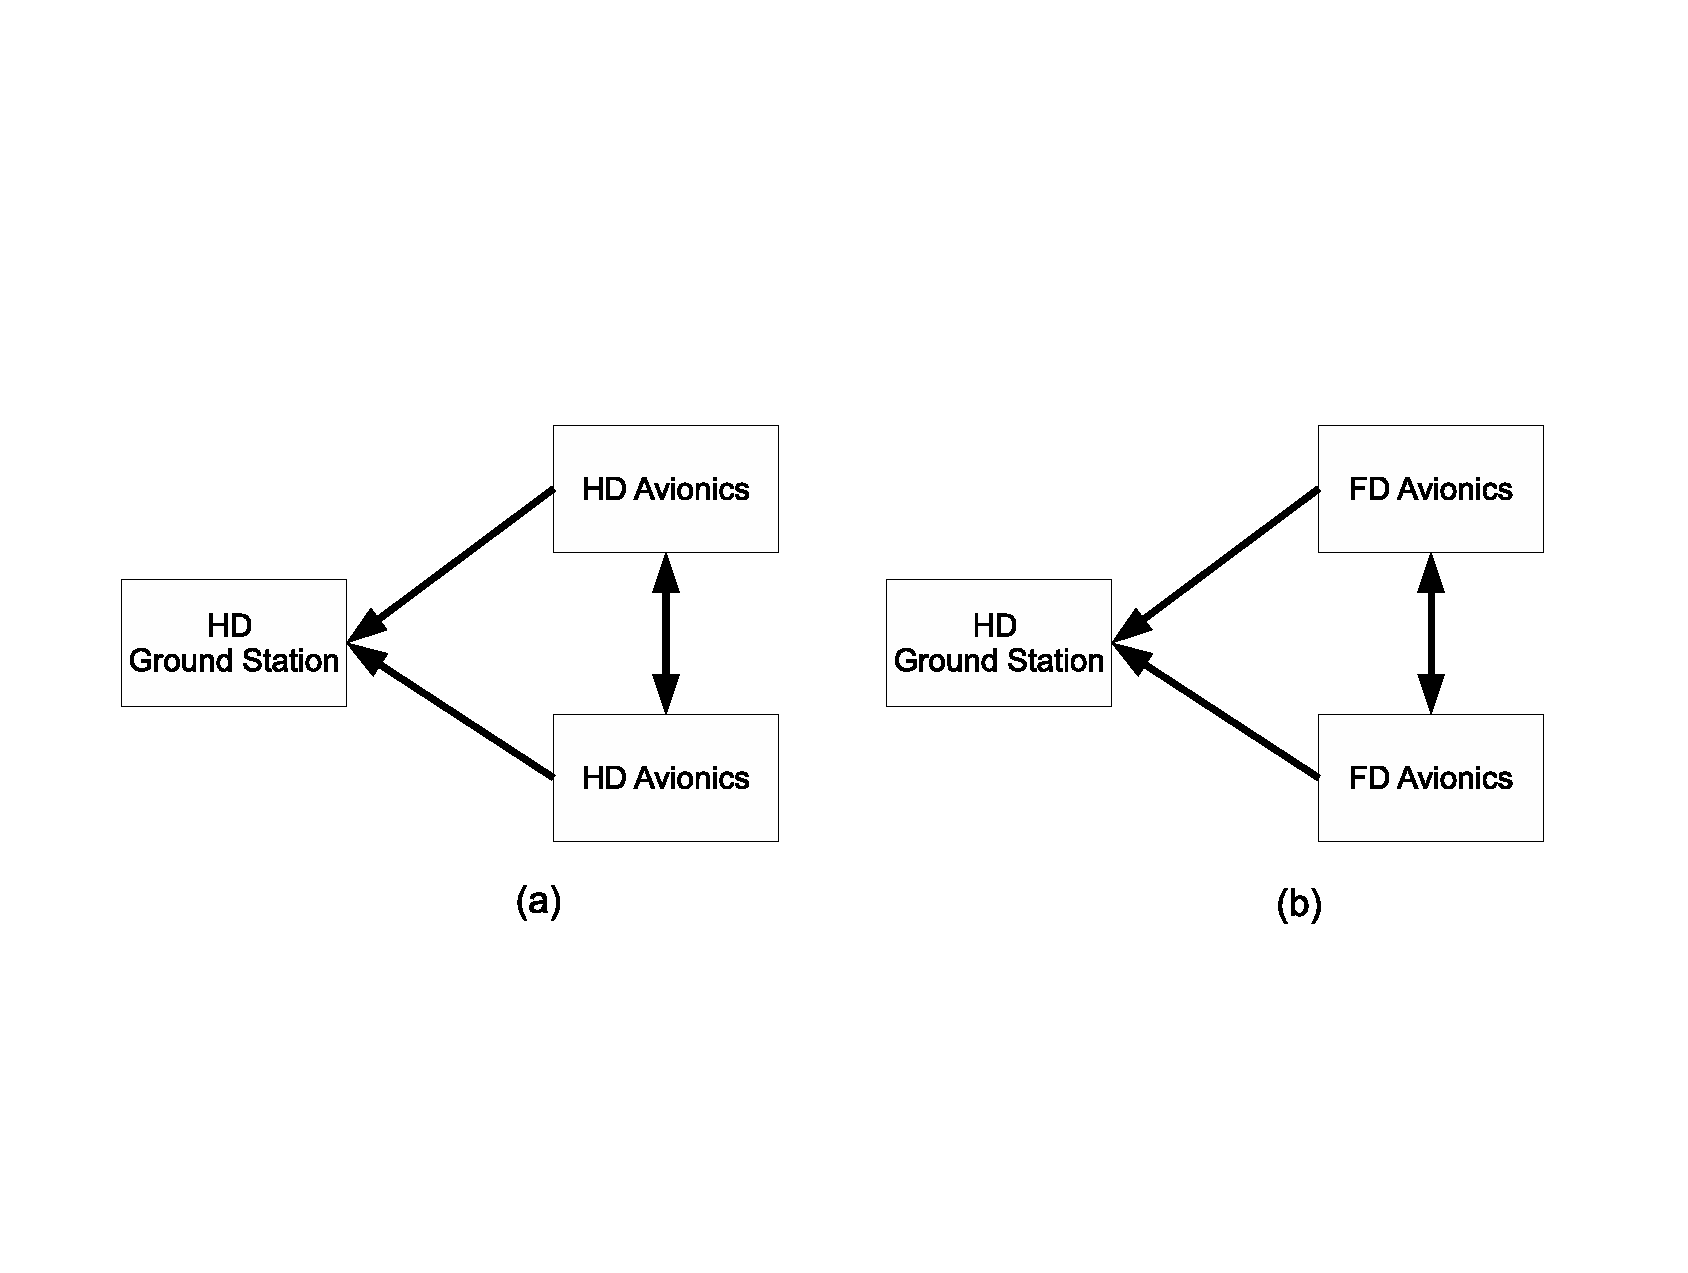
\includegraphics [width=0.8\columnwidth]{chap2_fig/chap2_hd_gs_system_model.eps} 
\vspace{-2cm}
\caption{Multi-user system model with a HD ground station and (a) HD receivers or (b) FD receivers.}
%\vspace{-0.5cm}
\label{fig:chap2_hd_gs_system_model}
\end{figure}

Apart from the techniques discussed earlier, several other spectral efficiency techniques, suitable for aeronautical communications, are available in the literature. However, the current work focuses on improving spectral efficiency in HD and FD-enabled ACSs over A/G links. In HD ACSs, the system model in Fig. \ref{fig:chap2_hd_gs_system_model}a is assumed, where the HD ACS, i.e., avionics, communicates with the ground station (GS). In FD ACSs, as seen in Fig. \ref{fig:chap2_fd_gs_system_model} and Fig. \ref{fig:chap2_hd_gs_system_model}b, self interference (SI) is experienced at the the FD transceivers due to the simultaneous signal transmission and reception. Also, interference at both HD and FD ACSs is also experienced due to the uplink nature of communication. 

Based on the system models seen in Fig. \ref{fig:chap2_fd_gs_system_model} and Fig. \ref{fig:chap2_hd_gs_system_model}, the current work focuses on advanced modulation schemes and In-Band Full-Duplex radio systems to boost spectral efficiency in HD and FD-enabled ACSs, which are practical and efficient spectrum utilization alternatives in aeronautical communications and is discussed in detail in the subsequent subsections.

\subsection{Modulation and Multiplexing Schemes for Aeronautical Communications}
\subsubsection{Modulation Schemes for Aeronautical Communications} 
% Disscuss relevance to aeronautical communications
Current A/G links rely on VDL-2 for data communications. However, the VDL-2 specification employs D8PSK as the modulation of choice to provide for a data rate of 31.5 kbps \cite{stacey2008aeronautical}. Evidently, the achievable data rate of VDL-2 is woefully inadequate if future data communication demands are to be met. To address the low data rate issue of current A/G links, advanced modulation schemes suitable for aeronautical communications can be implemented that either increases the number of bits transmitted per symbol or improves the reliability of communications, i.e., boost the spectral efficiency of ACSs. 

% Discuss techniques that increases the number of bits per transmitted symbol
The hierarchical modulation paradigm has been explored as an alternative to increase the number of bits per transmitted symbol by relying on the quadrant containing the QAM symbol as an additional domain to represent data bits \cite{jiang2005hierarchical,bae2008research} at the cost of signal detection complexity. Modified variants of PSK-based modulation have also been studied to increase the bits carried per symbol. In particular, transmitting additional bits through rotating the QPSK constellation in a specific direction was proposed by Liu et al. \cite{liu1992rotative}. Through the proposed method, an additional bit can be transmitted per QPSK symbol at the cost of higher receiver complexity. More recently, Hong et al. \cite{hong2015additional} proposed rotating the QPSK constellation after the transmission of each block of bits to convey additional bits. Although the detection complexity is not as substantial compared to \cite{liu1992rotative}, the proposed method only achieves a maximum of 16\% boost in throughput.

% Discuss BICM and SSD as techniques that increases reliability
% Present open problems related to aeronautical communications if possible
Apart from increasing transmission rates, enhanced modulation techniques have also been extensively studied to improve reliability. For instance, Bit Interleaved Coded Modulation (BICM) was first proposed by \cite{zehavi19928} to improve the reliability transmissions over Rayliegh fading channels. In particular, the transmitter performs interleaving at the bit level before modulation and vice versa at the receiver \cite{zehavi19928,caire1998bit,li2002bit,zhan2017differential}. BICM has since been extensively studied, with different decoding methods proposed \cite{li2002bit,abotabl2017broadcast} and evaluation over multipath Rayleigh channels conducted \cite{zhan2017differential}. Nonetheless, the increase in reliability for BICM comes at the cost of reduced euclidean distance \cite{li2002bit}.

Signal Space Diversity (SSD), i.e., modulation diversity, is also another technique that has been widely studied to improve communications reliability. SSD was first proposed by Boutros and Viterbo \cite{boutros1998signal} where the in-phase and quadrature phase components of a symbol are rotated and interleaved. The idea is to separately transmit the in-phase and quadrature phase components over a fading channel to diminish the impact of fading \cite{boutros1998signal}. By far, studies pertaining to SSD have looked at code design \cite{mohammed2012modulation} and performance analysis over Nakagami-$m$ \cite{lu2012bit} and Rayleigh \cite{sokun2017spectrally} fading channels. These analysis are useful since Nakagami-$m$ and Rayleigh can be encountered in aeronautical communications. However, suitable code designs for aeronautical communications and the impact of imperfect channel knowledge, particularly for various flight scenarios where Rician fading channels are expected, are open problems that must be addressed.

\subsubsection{Multiplexing Schemes for Aeronautical Communications}

An alternative to meet demands for rising data traffic stemming from aeronautical communications is the non-orthogonal multiple access (NOMA) paradigm. NOMA has been proposed as a next-generation multiple access candidate \cite{dai2015non} in 5G cellular communications. As spectral efficiency is a vital issue that must be addressed in 5G, NOMA, when compared to orthogonal multiple access (OMA) methods, offers spectral efficiency boosts whilst allowing massive connectivity \cite{dai2015non}. Conventional OMA methods such as Frequency Division Multiple Access (FDMA), Time Division Multiple Access (TDMA) and Code Division Multiple Access (CDMA) have traditionally been used to segregate users in terms of channel frequencies (e.g. spectral resources), timeslots or codes. 

However, OMA techniques inherently causes inefficient utilization of spectral resources as users have dedicated resources at the moment of transmitting or receiving signals. NOMA, on the other hand, allows multiple users to simultaneously share the same spectral resources. This is done by allowing an acceptable amount of interference from users simultaneously multiplexed to the same set of spectral resources \cite{dai2015non}. The NOMA paradigm can be well suited for adaptation for aeronautical communications. Interference from nearby aircrafts or ground stations can be canceled while accommodating a large number of aircrafts in the same airspace that are transmitting data via A/G or A/A communication links. To enable resource multiplexing, NOMA techniques can be broadly categorized as Power Domain Multiplexing (PDM) or Code Domain Multiplexing (CDM). 

\begin{figure} []
\centering
\vspace{-0.7in}
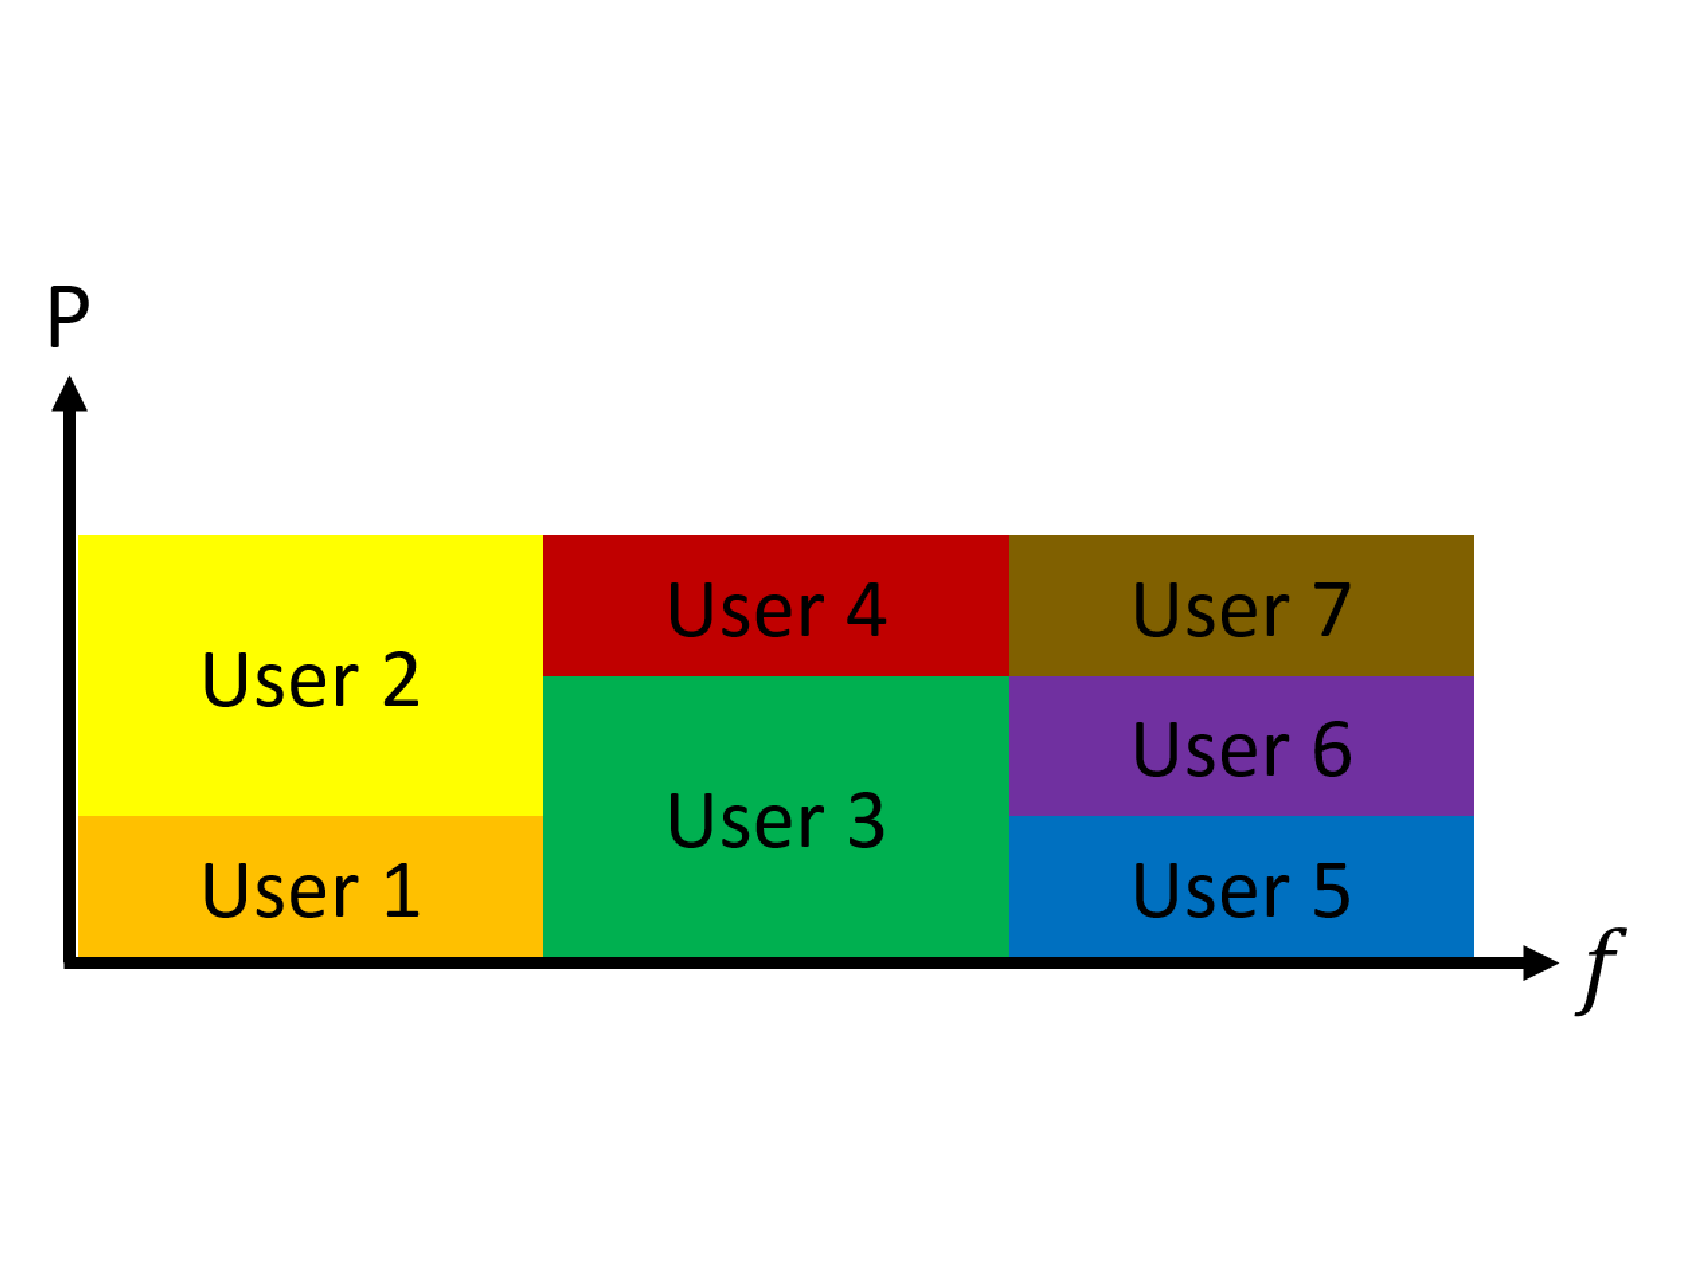
\includegraphics [width=0.6\columnwidth]{chap2_fig/NOMA_fig1.eps}  %ZICRSystemModel.eps} % {LAR.eps}\columnwidth   [width=2\columnwidth] 
\vspace{-0.8in}
\caption{Users in power domain multiplexing are partitioned using transmission power levels.}
\label{fig:6}
\end{figure}

In PDM-NOMA, signals are transmitted on the same frequencies using different power levels (Fig. \ref{fig:6}). This method of PDM is known as basic NOMA and was discussed by Saito et al. in \cite{saito2013non}. In particular, basic NOMA was applied for a downlink scenario involving two users, user one and user two with message signals $x_1$ and $x_2$ respectively and one base station. The base station transmits signal $y=x_1+x_2$ to all users simultaneously, with the sum of the transmit powers subjected to power constraints. To recover the signals, the users employ Successive Interference Cancellation (SIC) \cite{saito2013non}. 

Assuming that user 1 has less interference than user 2, user 1 will recover $x_1$ before subtracting $x_1$ from $y$. User 2 will then recover $x_2$ from $y$ after user one recovers $x_1$ \cite{saito2013non}. In general, SIC is used by users for signal detection, based on SINR measurements that is relative to all other nearby users. It was noted by Saito et al. \cite{saito2013non} that the power allocation ratio affects effective user throughput. To address this, flexible RRM is needed to take full advantage of this PDM technique. Similarly, Higuchi and Kishiyama \cite{higuchi2013non} proposed a beamforming PDM technique for MIMO LTE networks. In particular, the proposed technique combined beamforming and SIC for PDM-NOMA. It was however, noted by Song and Wang \cite{song2016comparison} that the main problems concerning SIC is the user delay and the potentially severe error propagation.

In contrast, techniques based on CDMA have been adopted for CDM-NOMA. One such method is Low Density Signature (LDS), seen in a paper by Hoshyar et al. \cite{hoshyar2008novel}. LDS is based on the LDPC spreading technique, that was originally developed for CDMA. The key idea behind LDS is to use sparse spreading sequences to reduce chip interference \cite{dai2015non}, {yuan2016non}. This is in contrast to dense spreading used in CDMA and is the key difference between LDS-based CDM-NOMA and conventional CDMA. In LDS, users recover their own messages by via a message passing algorithm (MPA) \cite{dai2015non}. Apart from LDS, Sparse Code Multiple Access (SCMA) has been explored as an alternative to LDS for CDM-NOMA by Nikopour and Baligh \cite{nikopour2013sparse}. Similar to LDS, SCMA relies on sparsely populated code words form via multi-dimensional constellations for non-orthogonal access \cite{yuan2016non}. Specifically, each user is assigned a sparsely coded codebook and data streams from each user are encoded via the respective codebooks before transmission. At the receiver, user detection is achieved via a MPA. Although both LDS and SCMA enable multi-user non-orthogonal access, the main limitation of both techniques is scalability \cite{yuan2016multi}.

\begin{figure} [!htpb]
\centering
\vspace{-0.6in}
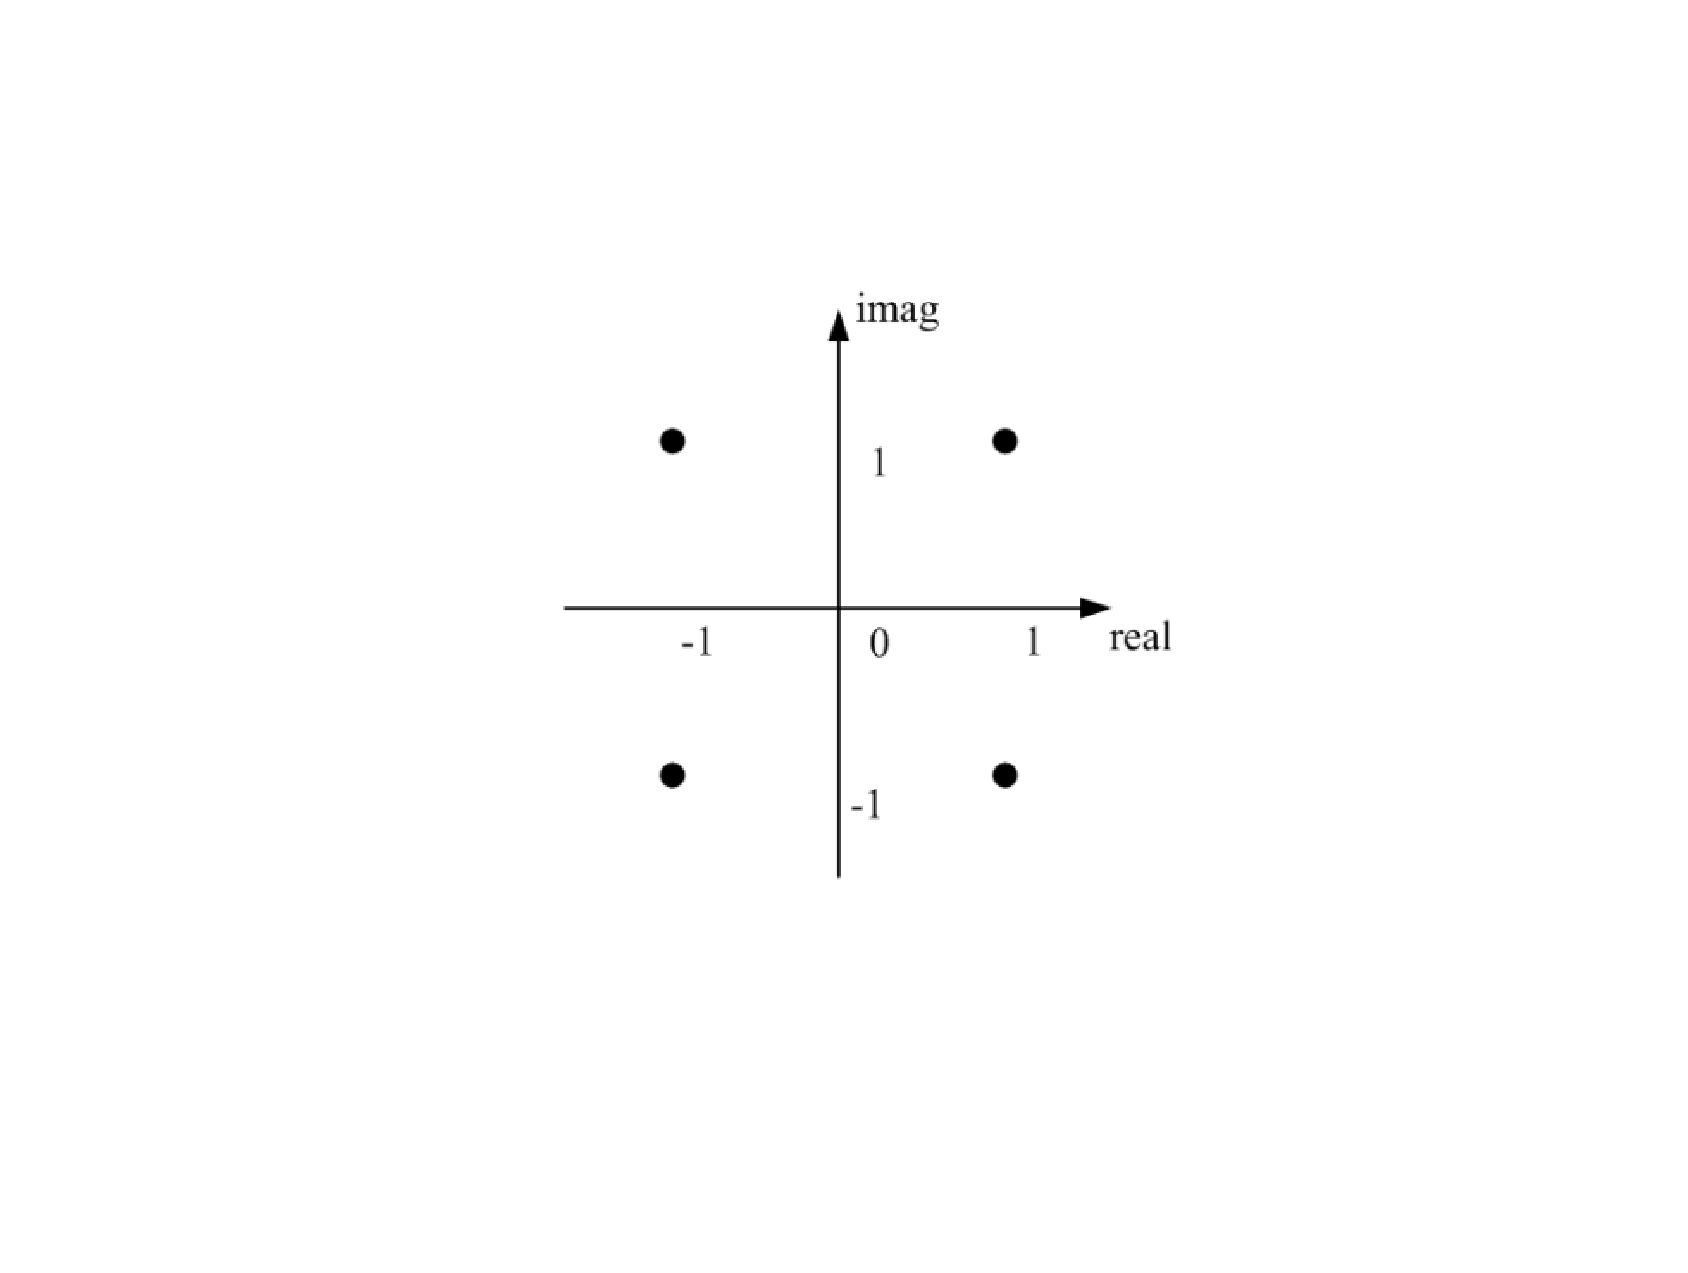
\includegraphics [width=1\columnwidth]{chap2_fig/NOMA_fig2.eps}  %ZICRSystemModel.eps} % {LAR.eps}\columnwidth   [width=2\columnwidth] 
\vspace{-1.5in}
\caption{A complex valued codeword constellation with 4 elements in MUSA. \cite{yuan2016multi}}
\label{fig:noma_fig2}
\end{figure}

An alternative for CDM-NOMA is Multi User Shared Access (MUSA), which was  in \cite{dai2015non}, \cite{yuan2016multi}. In MUSA, short length complex-valued codewords are used to spread user signals before transmission  \cite{yuan2016multi}. The complex valued codewords are constructed from complex valued constellations, with each codeword element picked from the constellation (Fig. \ref{fig:noma_fig2}). User overloading is thus accomplished by increasing the length of the codeword. For a codeword with length of $K$, there will be $4^K$ codewords available thus enabling scalability \cite{yuan2016non}. At the receiver, codeword-level SIC is employed to differentiate user messages. Although MUSA is more scalable then LDS and SCMA, the message recovery process in MUSA introduces the risk of error propagation due to SIC at the receiver. A summary of the discussed NOMA approaches is presented in Table \ref{table:noma}.

\begin{table}[]
\centering
\caption{Summary of discussed NOMA approaches}
\label{table:noma} \scalebox{0.9}{
\begin{tabular}{ccc}
\hline
\textbf{References}					& \textbf{Description}		 			& \textbf{Spectral Efficiency Metric(s)} \\ \hline \hline
\cite{saito2013non} 				& Basic NOMA SIC for PDM-NOMA   & Throughput                             \\ 
\cite{higuchi2013non}       & Beamforming SIC for PDM-NOMA  & Throughput                  \\ 
\cite{hoshyar2008novel}			& LDS for CDM-NOMA							& BER                                    \\
\cite{nikopour2013sparse}		& SCMA for CDM-NOMA							& BER                                    \\
\cite{yuan2016multi}				& MUSA for CDM-NOMA							& BER                                    \\ \hline
\end{tabular}}
\end{table}

%Non-Orthogonal Multiple Access (NOMA), on the other hand, is an alternative technique that can be adopted for spectral efficiency improvements in aeronautical communications. NOMA has been proposed as a next-generation multiple access candidate \cite{dai2015non} in 5G cellular communications. As spectral efficiency is a vital issue that must be addressed in 5G, NOMA, when compared to OMA methods, offers spectral efficiency boosts whilst allowing massive connectivity \cite{dai2015non}.
%
%NOMA allows multiple users to simultaneously share the same spectral resources by allowing an acceptable amount of interference from users simultaneously multiplexed to the same set of spectral resources \cite{dai2015non}. To enable resource multiplexing, NOMA techniques can be broadly categorized as Power Domain Multiplexing (PDM) or Code Domain Multiplexing (CDM).
%
%The NOMA paradigm can be well suited for adaptation for aeronautical communications. PDM-NOMA for instance, can take advantage of the fact that aircrafts on a flight path can be separated by vast distances (e.g. 10km and above). When path loss is considered, interfering signals from nearby aircrafts or ground stations is diminished. Thus, PDM-NOMA can be adopted for both A/G and A/A communications scenarios. CDM-NOMA can also be adopted for aeronautical communications, particularly in congested airspace where a large number of aircrafts are transmitting data via A/G or A/A communication links. In such a scenario, spectral efficiency is improved through simultaneous transmissions achieved via Multi User Shared Access (MUSA) \cite{dai2015non}, \cite{yuan2016multi} or even Sparse Code Multiple Access (SCMA) \cite{nikopour2013sparse}. Interference with legacy aeronautical communications can also be managed if PDM-NOMA or CDM-NOMA techniques are used in combination with D2D/CR related approaches.

\subsubsection{Open Research Problems for Modulation and Multiplexing Schemes in Aeronautical Communications}

The spectral efficiency of ACSs can be improved through suitable modulation schemes. With the current VDL-2 scheme providing low data rates for A/G links, modulation techniques that can transmit more bits per symbol effectively, with simple transceiver designs, can be further investigated. BICM can also be further explored for aeronautical communications usage. In particular, performance analysis of BICM over multipath channels are limited \cite{zhan2017differential}, particularly for combinations of Rician and Rayleigh fading which are expected in aeronautical communications, and can be studied in future works. For SSD, code designs that are suitable for aeronautical communications and the impact of imperfect channel knowledge, particularly for various flight scenarios where Rician fading channels are expected, are also open research problems that must be addressed.

NOMA approaches can also go a long way towards improving the spectral efficiency of ACSs. Although concepts such as frequency reuse, have been applied for aeronautical communications e.g. VDL-2 systems \cite{ribeiro2014framework}, there is further scope to study the feasibility of new NOMA methods for aeronautical communications. By enabling simultaneous sharing of the same frequency band, NOMA provides the capability to support simultaneous transmissions from multiple users in the same channel. When applied to ACSs, NOMA can effectively help to address the scarcity of aeronautical spectrum for communications. 

However, the major downside to such an approach is the inevitable introduction of interference to all NOMA users. In the aeronautical context, this translates to interfering with A/G or even A/A communications. In the worst case, the transmissions of legacy systems in the same band e.g. VHF or L-band, can also be affected. In this aspect, much work will have to be done in the aeronautical context to quantify potential levels of interference to other aircrafts and legacy systems. This is on top of improving PDM-NOMA or CDM-NOMA techniques to reduce delays, error propagation and complexity, which are still open research problems. Finally, future work can also for instance, study the feasibility of incorporating frequency reuse into PDM-NOMA for aeronautical communications.

\subsection{In-Band Full-Duplex Radio Systems for Aeronautical Communications}

% Disscuss relevance to aeronautical communications
The emerging field of In-Band Full-Duplex (IBFD) radio systems can be a direct solution to improve the spectral crunch faced by the aviation community. From the aeronautical communications perspective, IBFD systems enable ACSs, e.g., VDL-2, AeroMACS, LDACS-1 or LDACS-2, the capability to simultaneously transmit and receive signals on the same channel. Therefore, ACSs operating in FD mode can achieve up to twice the spectral efficiency compared to operating in HD mode. Furthermore with proper signal processing techniques, interference and congestion on the aeronautical spectrum between legacy, existing and FD-enabled ACSs can be managed. However, many technical challenges related to interference cancellation/management must be tackled before any aeronautical IBFD communications system can be made feasible.

\subsubsection{SI Cancellation Architectures and the Associated Considerations in Aeronautical Communications}
% Discuss SI technical hurdle and related SI cancellation literature in FD systems
\begin{figure} []
\centering
\vspace{-0.7in}
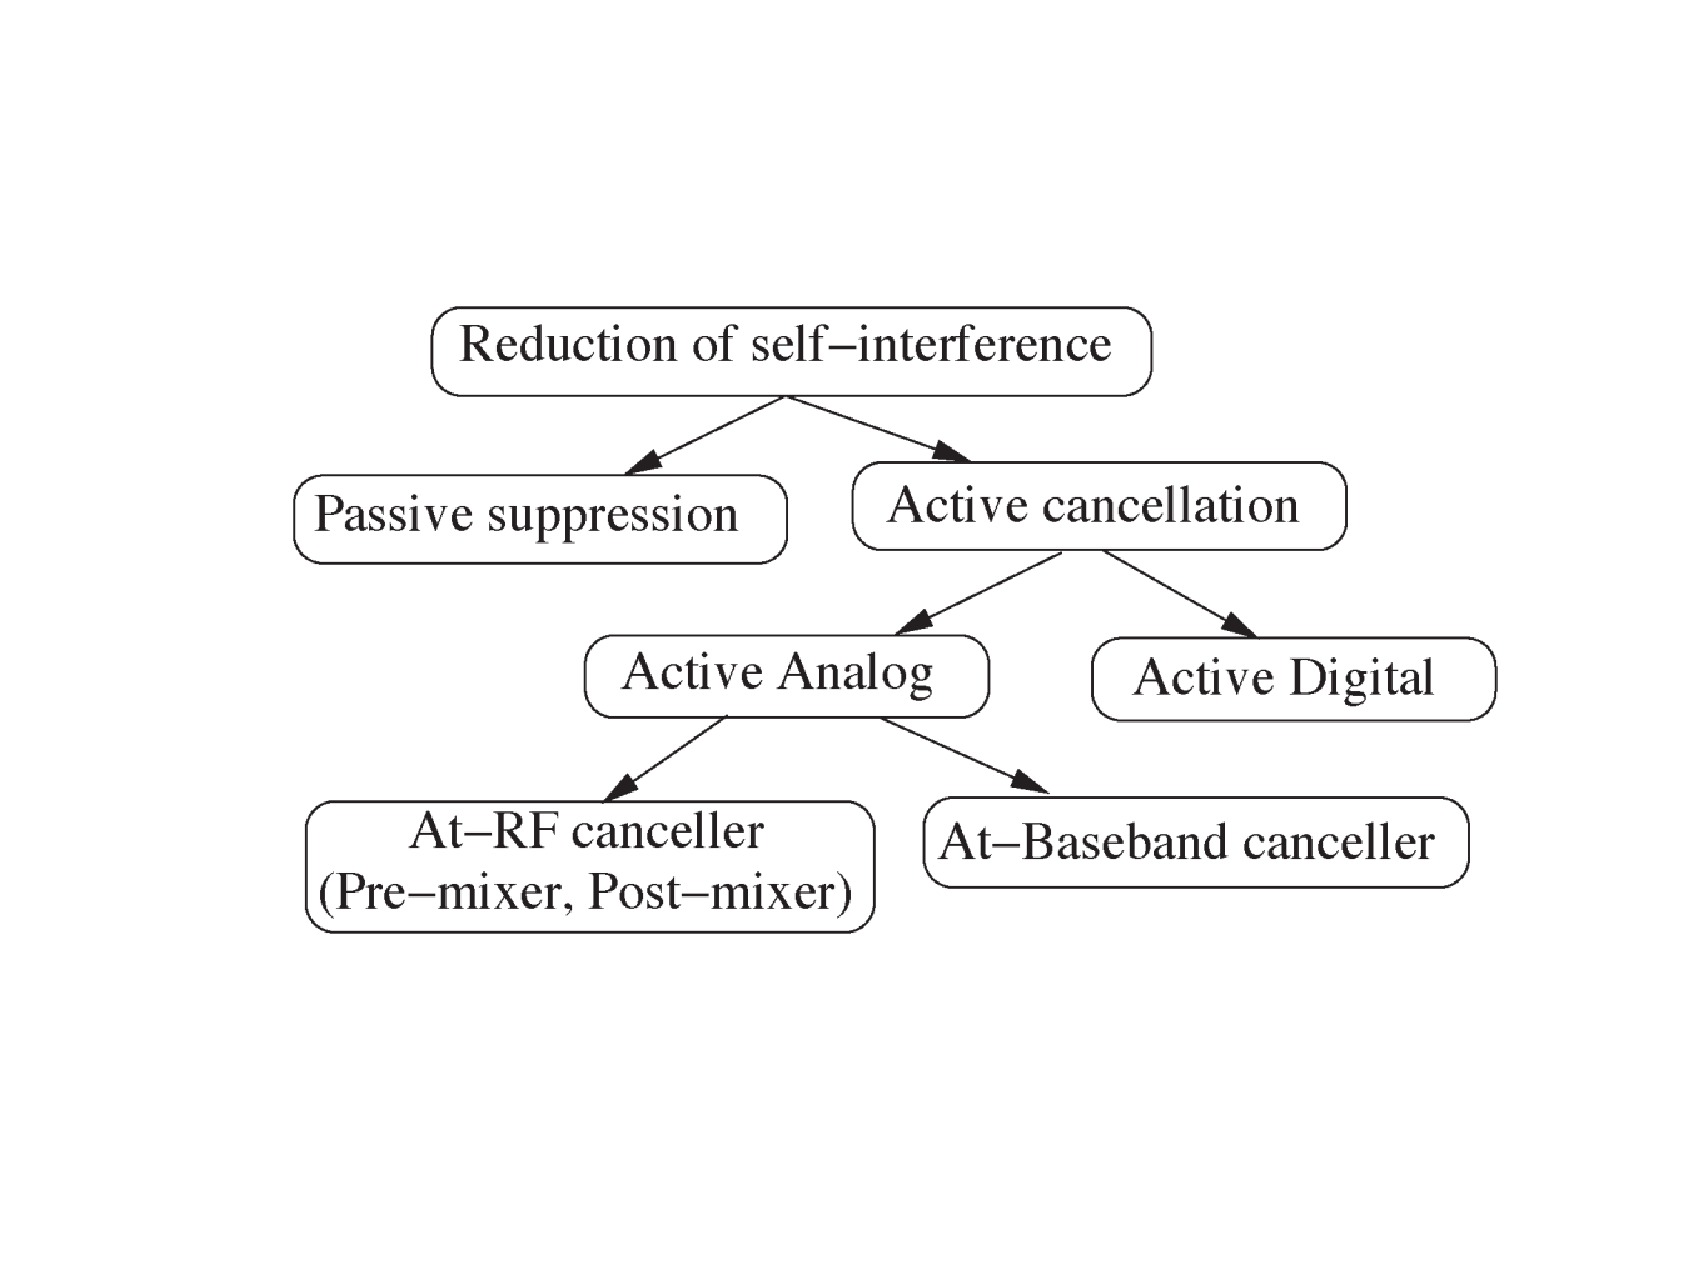
\includegraphics [width=0.7\columnwidth]{chap2_fig/IBFD_fig2.eps} 
\vspace{-0.8in}
\caption{Overview of SI mitigation architectures. \cite{sahai2013impact}.}
\label{fig:IBFD_2}
\end{figure}

One of the major technical hurdles in IBFD systems is the inherent introduction of self interference (SI). A practical IBFD system requires a sufficient level of SI mitigation before communications can become feasible. In this aspect, SI mitigation architectures can be categorized into either passive suppression or active cancellation \cite{sahai2013impact} (Fig. \ref{fig:IBFD_2}). The former entails SI mitigation via antenna separation (separate antenna IBFD systems) \cite{duarte2014design,ahmed2012simultaneous} or circulator isolation (shared antenna IBFD systems) \cite{bharadia2013full,huberman2015mimo} while the latter cancels SI either in the analog or digital domain. 

Active analog/digital SI cancellation architectures are further categorized as pre-mixer, post-mixer or baseband cancelers. A mixture of pre, post and baseband cancelers in the same architecture is also possible. In a pre-mixer canceler, the processing of the cancellation signal is performed before the RF mixer, e.g., having a parallel radio chain \cite{ahmed2015all}. Likewise, a post-mixer canceler processes the cancellation signal after the RF mixer, e.g., Balun (Balance/Unbalance) cancellation \cite{jain2011practical} while a baseband canceler processes the canceling signal at the baseband level.

% Discuss open problems related to SI mitigation
It should be noted that digital and analog SI cancellation both experience unique limitations \cite{sahai2013impact}. In digital SI cancellation, the strength of the resultant SI signal before it enters the ADC is high. Consequently, SI mitigation becomes ineffective since the SI signal will still be above the receiver noise floor after digital SI cancellation due to limited ADC dynamic range \cite{sabharwal2014band}. In analog SI cancellation, SI mitigation will require complex hardware \cite{everett2016softnull}, thus potentially increasing the physical size of transceivers and contributing to overall size, weight and power requirements for FD-enabled avionics. 

On top of the associated limitations for both digital and analog SI cancellation, residual SI will also be present in the form of phase noise. The residual SI is a result of imperfect SI channel estimation at the FD transceiver \cite{sahai2013impact} and it can be the limiting factor in practical IBFD systems. In addition, suitable SI mitigation architectures of IBFD systems (e.g. active or passive) will need to be investigated to determine a suitable architecture for aeronautical usage, on top of accurate theoretical modeling of SI signals and multipath fading effects in an aeronautical channel e.g. Rician or Rayleigh fading environments \cite{haas2002aeronautical}.

\subsubsection{Hybrid-Duplex Systems for Aeronautical Communications}
% Discuss HBD systems as a way to transition towards a newer generation of FD-enabled ACSs
Apart from suitable SI mitigation architectures and the associated considerations for aeronautical communications, transiting towards a new generation of FD-enabled ACSs is likely to be disruptive as legacy HD ACSs must first be replaced. To ease the transition from legacy HD to a FD-enabled ACS, a hybrid-duplex (HBD) ACS consisting of HD and FD aircrafts/ground stations, e.g., Fig. \ref{fig:chap2_fd_gs_system_model}, is a viable alternative. 

Already, HBD systems have been seen in cognitive radio systems \cite{li2014linear} and cellular systems \cite{yin2013full,jang2015spatial,cirik2016robust} where nodes operating in either HD or FD have been studied. The main obstacle in such a HBD system is the inherent SI as a result of simultaneous signal transmission and reception. As a result, sufficient levels of SI mitigation must be achieved to enable the co-existence of multiple ACSs operating on the same frequency. In this aspect, concepts related to NOMA can be adapted for FD operations. Future studies can look at the suitability of incorporating Successive Interference Cancellation (SIC) from power-domain NOMA \cite{yan2015receiver}, \cite{huang2016full}, \cite{ali2016dynamic}, \cite{zhang2016full} into multi-user IBFD wireless systems. Other studies can also look at using code-domain NOMA concepts such as MUSA or SCMA \cite{yuan2016multi}, \cite{nikopour2013sparse}. 

Apart from SI, HBD systems must also manage interference from nearby HD nodes, e.g., HD avionics, as seen in Fig. \ref{fig:chap2_fd_gs_system_model}a. Interference management strategies have long been an area of active research in the literature, particularly from the information theoretic perspective. For instance, studies investigating interference management approaches that do not consider any inherent structure in the interference, such as interference avoidance, have been noted \cite{qu2014understanding}. Such interference avoidance strategies, which are typically based on either random access, e.g., contention-based channel access, or deterministic access, e.g., orthogonal multiple access, hinders spectral efficiency \cite{qu2014understanding,weber2007transmission}. Therefore, exploiting the structure of interference, i.e., interference management, has been the topic of keen research interest in recent years \cite{qu2014understanding} to achieve better performance \cite{weber2007transmission} and spectral efficiency in multi-user systems. 

In aeronautical communications, the distances between aircrafts affects the level of interference experienced at the HD avionics. Long separation distances between aircrafts results in weak interference scenarios and vice-versa. Accordingly, suitable interference management techniques must be employed for different interference scenarios. For weak interference scenarios, it has been known that the optimal interference management strategy is to treat interference as noise, i.e., interference ignorant (II) \cite{annapureddy2009gaussian,zahavi2017cooperation} detector. In contrast, decoding and then removing interference from the received signal, i.e, successive interference cancellation (SIC) detector, is an effective interference management strategy in strong interference scenarios \cite{qu2014understanding,weber2007transmission}. The joint detection (JD) strategy is also another effective interference management strategy when the interfering signal is sufficiently strong \cite{zahavi2017cooperation,zhou2015mac,shubhi2017joint,blomer2009transmission}. In particular, the joint detector is optimal from the sum-rate perspective, when interference is sufficiently strong, for an additive white Gaussian noise channel \cite{zahavi2017cooperation} at the cost of computational complexity \cite{zhou2015mac,shubhi2017joint}.

To measure the effectiveness of the various interference management strategies in HBD systems, outage probability can be analyzed. In the literature, outage probability for many statistical distributions has been extensively studied. For the II detector, outage probability for Gamma distributed signals \cite{yao1992investigations}, composite fading consisting of exponentially distributed signal-of-interest (SOI) and squared ${\mathcal{K}}$-distributed interfering signals \cite{bithas2015mobile}, and non-centered Chi-squared distributed signals \cite{rached2017unified} are available in closed-form. 

For the SIC detector, closed-form outage probability expressions for combinations of non-centered Chi-squared, exponential or Gamma distributed SOI with exponentially distributed interfering signals were studied in \cite{hasna2003performance,romero2008receive}. However, both \cite{hasna2003performance} and \cite{romero2008receive} assumed partial SIC where at least one interferer remain after interference cancellation and thus, performance analysis involving full SIC cannot be obtained. The outage probability of full SIC with exponentially distributed signals was analyzed in \cite{zhang2017full} and to the best of our knowledge, similar outage analysis for non-centered Chi-squared distribution is not yet available in the literature. Finally, for the joint detector, outage analysis is only available for exponentially distributed signals, as presented in \cite{narasimhan2007individual}, and similar studies involving non-centered Chi-squared distribution are unavailable in the literature.

Finite SNR diversity gain and finite SNR diversity-multiplexing trade-off (DMT) are also metrics that can measure the effectiveness of the various interference management strategies in HBD systems. For fixed transmission rate systems, reliability is quantified through finite SNR diversity gain by computing the outage probability decay rate at a fixed SNR \cite{shin2008diversity}. Reliability in variable transmission rate systems is similarly quantified through finite SNR DMT, with the transmission rate, i.e., multiplexing gain, taken into consideration \cite{narasimhan2006finite}. 

Although diversity gains have long been analyzed at asymptotic SNRs, a gradual shift in research interest towards the low-to-moderate SNR regime has been seen due to the practical relevance in the evaluation of system performance. In particular, wireless systems typically operate at low-to-moderate SNR regimes, and through finite SNR analysis, changes in outage probability behavior can be observed \cite{shin2008diversity}. Knowing a system's outage probability behavior at low-to-moderate SNR regimes is essential in providing accurate system performance analysis as it reveals the SNR needed before a particular level of reliability, i.e., Quality-of-Service (QoS), is attainable through effective code designs, e.g., turbo codes, low-density parity-check codes and space-time codes \cite{narasimhan2006finite}. Finite SNR analysis also allows the identification of the multiplexing gain region (MGR) \cite{karmakar2012generalized}. The MGR indicates the range of multiplexing gains for which non-zero diversity gains is attainable in a multi-user channel. In aeronautical communications, MGRs enable system designers to determine the QoS requirements of ACSs and extensive analysis on this topic is unavailable in the literature.

\subsubsection{Integration of In-Band Full-Duplex Cognitive Radio Systems for Aeronautical Communications}

One of the key reasons behind the shortage of available spectrum for aeronautical communications stems from the inefficient allocation of radio channels \cite{jacob2016cognitive}. In particular, radio channels used in aeronautical communications are often assigned to specific geographical areas \cite{jacob2016cognitive} or ACSs \cite{jamal2017fbmc}, e.g., distance measuring equipment (DME), on a permanent basis. The static allocation of the aeronautical spectrum exasperates the issue of spectral efficiency due to inefficient utilization of spectral resources, where spectrum utilization as low as 5\% has been reported \cite{jacob2016cognitive}. In the L-band, the static allocation of the aeronautical spectrum has resulted in unused spectrum, i.e., white space, between adjacent DMEs \cite{jamal2017fbmc}. Although LDACS-1 and LDACS-2 can be deployed to operate within the white space \cite{schnell2014ldacs,jamal2017fbmc}, spectral efficiency can be further improved through the introduction of FD-enabled cognitive radio (CR) systems in aeronautical communications.  

% elaborate more on what kind of channel models we can use, whether the SU or PU operates in FD, which node (GS or AS?) utilizes CR.
Unlike in HD CR systems, FD-enabled CR systems have the capability to simultaneously transmit signals while sensing the spectrum \cite{amjad2017full}. CR applications in the context of aeronautical communications have been studied in the literature for A/G \cite{wang2010cognitive,zhang2015aeronautical} and unmanned aerial vehicle (UAV) communications \cite{saleem2015integration,chen2011collaborative}, with ground stations (GSs) and air-stations (ASs) alike playing the role of either primary users (PUs) or secondary users (SUs).

The utilization of the white space also differs from HD CR systems. In the underlay mode of operation, the transmissions of the SUs and PUs in HD CR systems are controlled such that the interference experienced by the PUs is sufficiently low \cite{amjad2017full}. The underlay mode of operation in FD-enabled CR systems is similar except that both PUs and SUs transmit on the same spectrum \cite{amjad2017full,gaafar2017underlay}. For the overlay mode of operation, SUs in HD CR systems vary transmission characteristics to avoid interfering with PUs on the same frequency band \cite{amjad2017full}. However, in FD-enabled CR systems, PUs and SUs simultaneously transmit on the same frequency and SUs vary transmission characteristics to reduce SI \cite{amjad2017full,amin2017overlay}. In the interweave mode of operation, SUs only operate when the PUs are not transmitting for both HD and FD-enabled CR systems \cite{amjad2017full,liao2014listen}. The only difference between HD and FD-enabled CR systems in interweave mode is that SUs in the latter simultaneously sense and transmit signals, thus improving spectrum utilization. Finally, hybrid modes of operation are also possible in FD-enabled CR systems, e.g., in \cite{afifi2015incorporating} where SUs either sense-and-transmit or transmit-and-receive signals simultaneously.

The nature of FD-enabled CR systems enables the activities of the PUs and the SUs to be monitored much more effectively than HD CR systems. As such, interference management strategies used in HBD systems can be readily adopted to manage the interference between PUs and SUs. For instance, the II approach to interference management can be adopted for use in FD-enabled CR systems operating in underlay mode. Interference management strategies based on SIC and JD approaches can also be employed for FD-enabled CR systems operating in overlay mode. The performance analysis done for HBD systems, e.g., outage probability and finite SNR diversity gain, can also be applied in FD-enabled CR systems to gauge performance at both node and system level.

\subsubsection{Open Research Problems of In-Band Full-Duplex Systems for Aeronautical Communications}

% Discuss the potential open problems of FD-enabled ACS
Employing the in-band full-duplex paradigm to address spectral efficiency in aeronautical communications is a very attractive solution. As seen in this section, spectrum utilization can be twice as effective in FD-enabled systems than HD systems. From the aeronautical communications perspective, realistic performance analysis of FD-enabled ACSs must take into consideration scenarios involving an aircraft that is en route, landing, taking-off or parking. In addition, the impact of inter-aircraft interference and residual SI must be examined in detail, before a fair assessment of FD-enabled ACSs is made possible. To this end, outage probability and finite SNR diversity gain are effective metrics that can provide system designers with theoretical node and system level performance. These metrics can be adopted for both HBD systems and FD-enabled CR systems in aeronautical communications.

Outage probability computations for FD-enabled ACSs must involve aircrafts and GS communicating in en route, landing, taking-off or parking scenarios, where fading is encountered. Since inter-aircraft interference and SI are also present, outage probability expressions in an interference-limited environment consisting of either Rician fading, Rayleigh fading, or combinations of both, must be derived for interference management strategies based on II, SIC or JD. For Rician fading environments, closed-form outage probability expressions are only available in \cite{rached2017unified} for the II-based interference management strategy. For both SIC and JD interference management strategies in Rician fading environments, closed-form outage probability expressions are not available in the literature. 

In \cite{rached2017unified}, the authors proposed an innovative moment-based approach to evaluate outage probability by expressing the probability density functions (PDFs) of the SOI and the interfering signal into the power series equivalent for various statistical distributions. The same approach can also be extended to evaluate both the SIC and JD interference management approaches to potentially yield closed-form outage probability expressions, along with provisions of the necessary convergence tests. The resultant outage analysis can be used to determine the impact of residual SI and inter-aircraft interference at both node and system level and compared against HD ACSs. For various inter-aircraft interference levels, suitable interference management strategies can also be identified.

The closed-form outage probability expressions, in the form of power series, for the II, SIC and JD approaches can be used as platforms to derive closed-form finite SNR diversity gain expressions. In particular, the finite SNR diversity gains of fixed and variable rate ACSs can be quantified and analyzed in detail to determine reliability, i.e., QoS, under various inter-aircraft interference levels. From the derived closed-form finite SNR diversity gain expressions, the MGR of the II, SIC and JD approaches be plotted to reveal the respective range of supported QoS requirements for A/G and A/A communications.

The resultant conclusions from both outage and finite SNR diversity gain analysis can then be used to identify A/G or A/A communication scenarios in which FD-based ACSs either performs the same as, or outperforms HD-based ACSs. Furthermore, outage and finite SNR diversity gain analysis can be used to determine the upper and lower bound of BER performance for both FD-based and HD-based ACSs. Future studies can also look at simulating various modulation techniques such as BPSK, QPSK, 8-PSK, D8PSK and QAM to determine if any of these modulation techniques are well suited for FD operations. The incorporation of constellation rotation and its effects on BER performance can also be studied for both FD-based and HD-based ACSs. These studies can also identify the ideal operating scenarios for practical systems, e.g., identifying ideal scenarios for constellation rotation in ACSs.

\section{Summary}
With growing air traffic projected in the near future, the issue of spectral efficiency in aeronautical communications will be a critical problem that must be addressed in due time by the aviation industry. In this chapter, works pertaining to the state-of-the-art in aeronautical communications was surveyed, with AeroMACS, satellite communications and LDACS earmarked as candidate technologies for airport, remote and continental communications respectively. Techniques ranging from CR and D2D communications to NOMA and IBFD radio was also surveyed as potential methods to improve spectral efficiency in aeronautical communications. Finally, the possible adaptation of earlier highlighted spectral efficiency approaches to further improve spectral efficiency in the aeronautical context was presented as possible research opportunities in aeronautical communications. The feasibility of employing general spectral efficiency improvement techniques such as IBFD radio systems and NOMA was also discussed, with potential open research problems highlighted.





%---------------------------------------------------------------------------------
\chapter{Interference Management in Hybrid-Duplex Aeronautical Communication Systems}
\label{chap:interference_management_HBD_ACS}
%---------------------------------------------------------------------------------
\section{Introduction}

Thus far, the lack of spectrum has been discussed in the context of UAV communications. However, spectrum scarcity is also present in aeronautical communications involving manned aerial vehicles. In particular, between 2012 and 2032, air travel within the Pacific South East Asia region is projected to record a compounded annual growth rate of 5.3\% \cite{icao2016long}. This air travel growth trend exposes existing aeronautical communication systems (ACSs) to considerable strain due to demand for data communications from legacy, current, and future generation of avionics systems. Consequently, this places an additional strain upon existing Air-to-Ground (A/G) and Air-to-Air (A/A) aeronautical communication links on the congested aeronautical spectrum. With existing ACSs being unable to deliver the needed data capacity \cite{neji2013survey}, various communication technologies have been proposed to improve the capabilities of existing A/G and A/A links \cite{neji2013survey,ernest2016efficiency}. However, these solutions do not directly address the issue of spectrum utilization.\footnote{The work in this chapter has been published in \cite{ernest2019outage}.}

In this spirit, an HBD ACS, comprising HD air-stations (ASs) operating existing avionics systems with FD GSs, can be an alternative solution to the shortage of available spectrum currently faced by the aviation community. Changes to existing/legacy HD avionics systems currently on board aircrafts can be kept to a minimum in HBD-ACS, thus enabling HBD-ACS to be less disruptive to adopt. Wireless communication systems that have adopted the HBD paradigm include cognitive radio systems \cite{li2014linear} and cellular systems \cite{mohammadi2015full, jang2015spatial, cirik2018robust}. \textcolor{black}{With FD nodes experiencing SI, adopting effective SI mitigation strategies for HBD-ACSs enables spectrum scarcity to be addressed in the aviation industry}. In particular, multiple aircrafts and ground stations can communicate on the same aeronautical spectrum, providing motivation for this chapter.

\subsection{Related Literature}
Apart from SI at FD nodes, HD nodes in HBD systems also experience interference due to transmissions from other HD and FD nodes. In the literature, multiple interference management approaches have been presented. However, this chapter focuses on two widely known approaches where interference is either ignored, i.e., II detector, or successively canceled, i.e., SIC detector. 

To quantify the effectiveness of the II and SIC detectors, many related works in literature have attempted to determine the closed-form outage probabilities of these detectors under various fading models. Having a closed-form outage probability expression enables a system's packet error rate, i.e., link availability, to be analyzed if the transmitted signals span over one fading block \cite{lin2013outage}. For the II detector, closed-form outage expressions for Nakagami-$m$ fading \cite{yao1992investigations} and composite fading consisting of exponentially distributed SOI and squared ${\mathcal{K}}$-distributed interfering signals \cite{bithas2015mobile} have been noted. However, \cite{yao1992investigations} and \cite{bithas2015mobile} are only applicable to specific fading environments and may not be applicable for all aeronautical scenarios where Rician fading is experienced. To this end, a recent paper by Rached et al. \cite{rached2017unified} presented generalized outage probability expressions that apply to a wide variety of fading scenarios, including Rician fading.

For SIC detectors, multiple works on outage analysis have been noted. For instance, the outage probability of SIC has been investigated by Hasna et al. \cite{hasna2003performance} and Romero-Jerez and Goldsmith \cite{romero2008receive}, but these studies only considered partial SIC where at least one interfering signal remains after interference cancellation. A closed-form outage expression for SIC was presented by Weber et al. \cite{weber2007transmission} for nodes distributed via a Poisson point process. However, the work in \cite{weber2007transmission} did not consider fading and receiver noise in the signal model. Thus, the closed-form expressions are not directly applicable for aeronautical communications. In a recent paper by Zhang et al. \cite{zhang2017full}, outage probability expressions for a two-stage SIC detector were presented. Yet, the outage expressions are specific for Rayleigh fading scenarios and are not applicable to Rician fading scenarios that are common in aeronautical communications. From the mentioned studies, hitherto closed-form outage probability expressions for SIC detectors in Rician fading aeronautical scenarios remain an open problem.

Apart from outage probability, both finite SNR diversity gain and finite SNR DMT are metrics that can be used to measure the effectiveness of II or SIC detectors in fixed and variable transmission rate systems, respectively. In particular, both finite SNR diversity gain and finite SNR DMT quantify the slope of outage probability curves at a particular SNR \cite{shin2008diversity}, with the latter considering multiplexing gain \cite{narasimhan2006finite}. Finite SNR analysis can reveal outage deviation behaviors, which are not present at asymptotically high SNRs due to fading statistics \cite{shin2008diversity}. From a practical perspective, analyzing outage probability decay rates, i.e., finite SNR diversity gain, provides an accurate picture of a system's outage performance since wireless communication systems are typically designed to operate at low-to-moderate SNR ranges. It has also been pointed out by Narasimhan \cite{narasimhan2006finite} that finite SNR diversity gain analysis can be used to estimate the SNR needed to achieve a particular rate of error decay, that can be done through turbo codes or low-density parity-check codes. More crucially, outage probability and diversity gain can be used to gauge the upper and lower limits of a system's bit error rate performance \cite{zheng2003diversity,nabar2005diversity}. 

Finite SNR analysis for Nakagami-$m$ \cite{wang2012finite} and Rayleigh fading \cite{lin2013outage,yang2015efficient} scenarios have also been studied. However, the conclusions drawn in these studies are specific to Nakagami-$m$ and Rayleigh fading and are not fully applicable for ACSs since Rician fading scenarios, typically encountered in aeronautical communications, are not considered. Studies on finite SNR analysis for Rician fading channels have been seen. The impact of Rician $K$ factors on outage behavior and finite SNR DMT for MIMO systems was investigated by Narasimhan \cite{narasimhan2006finite} and Shin et al. \cite{shin2008diversity}. A recent paper by Heidarpour et al. \cite{heidarpour2017finite} saw finite SNR DMT analysis being applied to analyze the performance of a network coded cooperative communication system. Despite the noted studies, there is still room for further work on finite SNR DMT analysis for HBD-ACS.

\subsection{Relevance to Related Literature}
In this research, full interference cancellation is assumed for the two-stage SIC detector. This is unlike in \cite{hasna2003performance} and \cite{romero2008receive} where only partial SIC is assumed. In addition, the impact of interference on the proposed HBD-ACS is analyzed from the outage probability and finite SNR DMT perspective, which was not covered in \cite{li2014linear,cirik2018robust,yao1992investigations,rached2017unified,weber2007transmission,zhang2017full}. In contrast to \cite{shin2008diversity}, \cite{narasimhan2006finite} and \cite{heidarpour2017finite}, this work extends upon the outage and finite SNR DMT analysis framework to jointly identify interference scenarios for the proposed single-input-single-output equivalent HBD-ACS.

%%%%%%%%%%%%%%%%%%%%%%%%%%%%%%%%%%%%%%%%%%%%%%%%%%%%%%%%%%%%%%%%%%%%%%%%%%%%%%%%%%%%%%%%%%%%%%%%%%%%%%%%%%%%%%%%%%%%%%%%%%%%%%%%%%%%%%%%%
% Section 2 : System Model
\section{System Model}
\begin{figure} [tpb]
\centering
%\vspace{-1cm}
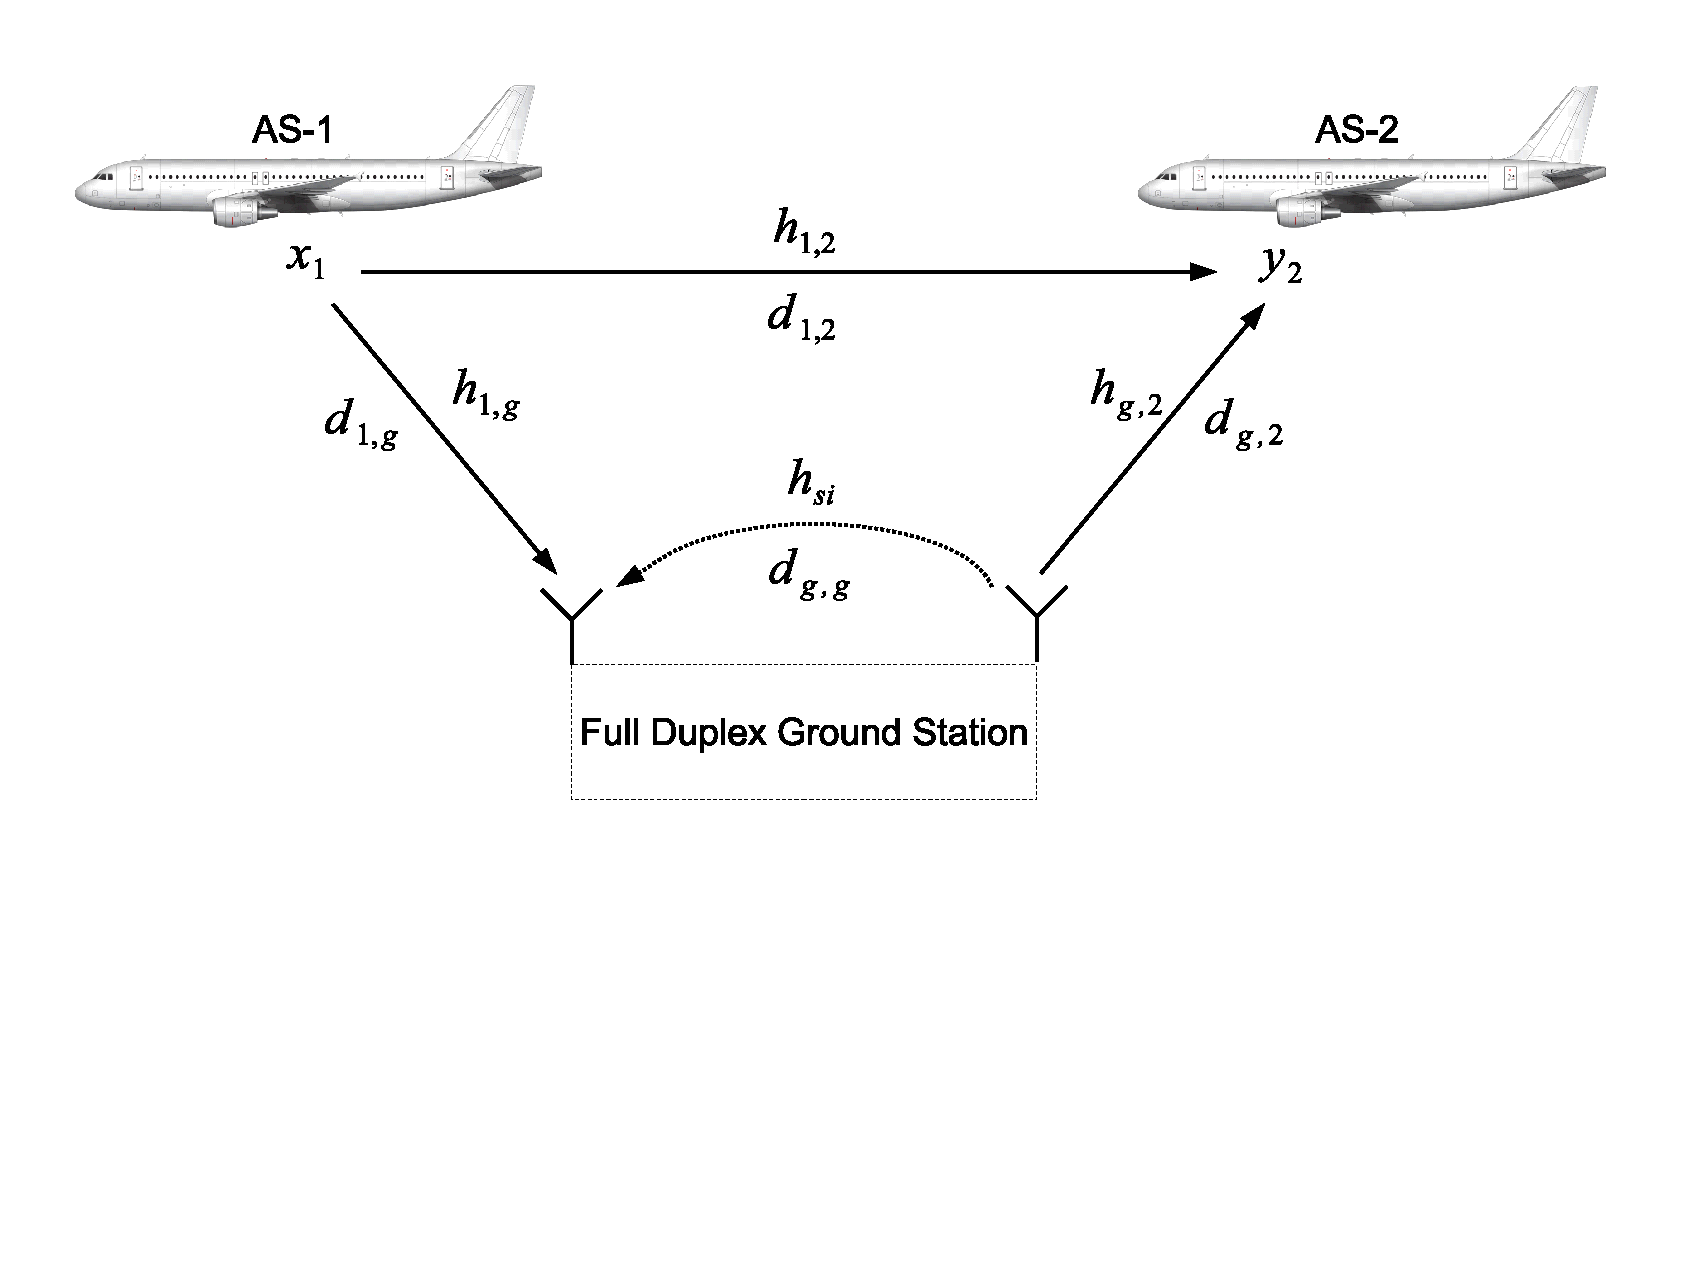
\includegraphics [width=0.6\columnwidth]{chap3_fig/block_diagram.eps} 
\vspace{-2cm}
\caption{Air-Station 1 (AS-1) and Air-Station 2 (AS-2) operating in HD mode while communicating with the FD GS.}
%\vspace{-1cm}
\label{fig:interference_management_HBD_ACS_1}
\end{figure}

In this chapter, A/G communications involving an FD-enabled GS node with two HD ASs in an A/G link is studied (Fig. \ref{fig:interference_management_HBD_ACS_1}). \textcolor{black}{\footnote{\textcolor{black}{The present chapter can be extended to consider an arbitrary number of uplink and downlink nodes. To enable the modeling and analysis of such multi-node networks, the signal model at the GS and also at the nodes will need to be modified. Furthermore, stochastic geometry tools, i.e., the BPP model, will need to be employed to accurately model the deployment of the nodes. These issues are addressed in Chapter \ref{chap:HBD_multi_UAV}, where new signal models that considers the BPP model are proposed for an HBD multi-UAV network.}}} Specifically, a scenario with Air-Station 1 (AS-1) transmitting signals to the GS while Air-Station 2 (AS-2) is receiving signals from the GS is assumed. For the HD transceivers at AS-1 and AS-2, a single-antenna configuration with separate transmit and receive radio frequency chains is assumed. In contrast, the FD transceiver at the GS is assumed to be configured with one transmit antenna and one receive antenna through separate radio frequency chains. Due to the fact that the GS node is FD-capable, the HD AS-1 and HD AS-2 simultaneously transmits and receives, respectively, signals on the same aeronautical spectrum (e.g. VHF, L-band) as the GS. Therefore, AS-1 interferes with communications at AS-2 when the latter receives signals from the GS.

The current research assumes an SI mitigation architecture with a shared local oscillator at the FD-enabled GS. Such a setup enables lower levels of phase noise to be experienced \cite{syrjala2014analysis}, \cite{li2018self}. As such, we only consider residual SI at the FD-enabled GS as a result of imperfect SI channel estimation and phase noise \cite{sahai2013impact}. Furthermore, the SI link ($h_{si}$) is modeled as a Rician fading channel to account for passive and active SI mitigation \cite{ahmed2015all}.\footnote{Depending on the degree of passive and active SI mitigation, the resultant SI channel ($h_{si}$) can be a Rician or Rayleigh fading channel \cite{ahmed2015all}. Thus, modeling $h_{si}$ as a Rician fading channel enables the degree of passive and active SI mitigation to be defined through the Rician $K$ factor.} Thus, an II detector is considered at the FD-enabled GS since signal detection is performed in the presence of residual SI.

Rician faded aeronautical communications channels in an en route scenario are assumed to provide a realistic evaluation of the HBD-ACS \cite{haas2002aeronautical,matolak2017air_suburban,yuan2018capacity}. Following the work in \cite{haas2002aeronautical} and \cite{yuan2018capacity}, the link between AS-1 and AS-2 is also modeled as a Rician fading channel. Accordingly, we assume that the ASs are communicating with the GS at cruising altitude, with the signal model based on \cite{sahai2013impact}. Also, the effect of Doppler shift is assumed to be compensated in this work \cite{lee2018uav}.\footnote{It is useful to note that Doppler shift is not a performance limitation in the upcoming L-band digital aeronautical communication systems (LDACS) standard \cite{jamal2017fbmc}.} A summary of important notations is given in Table \ref{table:interference_management_HBD_ACS_summary_impt_notations}.

\subsection{Ground Station}

Let $x_1[t]$ and $x_{gs}[t]$ be the signals transmitted by AS-1 and GS, respectively, and $h_{1,g}[t]$ be the channel from AS-1 to GS. Additionally, let $x_{si}[t]$ be the SI signal at GS and let $h_{si}$ be the SI channel gain. From the perspective of GS, $x_{si}[t]=x_{gs}[t]$. The received signal at GS can be written as 
%%%%%%%%%%%%%%%%%%%%%%%%%%%%%%%%%%%%%%%%%%%%%%%%%%%%%%%%%%%%%%%%%%%%%%%%%%%%%%%%%
\begin{eqnarray} \label{interference_management_HBD_ACS_y_gs}
y_{gs}[t] & = & \sqrt{\Omega_{X}}h_{1,g}[t]x_{1}[t] + \sqrt{\Omega_X\alpha_{g,g}} \cdot |\widetilde{h}_{si}|x_{si}[t] + \sqrt{\Omega_X\alpha_{g,g}}|h_{si}|\gamma_{\phi}w_{\phi}[t] + w_{g}[t],
\end{eqnarray}
%%%%%%%%%%%%%%%%%%%%%%%%%%%%%%%%%%%%%%%%%%%%%%%%%%%%%%%%%%%%%%%%%%%%%%%%%%%%%%%%%
where $\widetilde{h}_{si}$ is the error of the imperfect SI channel gain estimate, defined as $\widetilde{h}_{si}=h_{si}-\widehat{h}_{si}$, and $\widehat{h}_{si}$ is the imperfect estimation of the SI channel gain. In addition, let $\widetilde{h}_{si}$ be modeled as a zero mean, circularly symmetric complex Gaussian RV with variance $\epsilon$ to quantify the SI channel estimation error \cite{zlatanov2017capacity}. Modeling $\widetilde{h}_{si}$ as a zero mean Gaussian RV with variance $\epsilon$ enables the system to model the worst case residual SI \cite{zlatanov2017capacity}. Also, let $w_{g}[t]$ be the GS additive white Gaussian noise (AWGN) with zero mean and variance $\sigma^2_{g}$, and let the phase noise term $w_{\phi}[t]$ follow a Gaussian distribution with zero mean and unit variance, scaled by the scaling factor $\gamma_{\phi}$ \cite{sahai2013impact}.\footnote{The scaling factor $\gamma_{\phi}$ models the jitter present in oscillators due to hardware imperfections \cite{sahai2013impact}}

Let $\Omega_{X}$ be the average received signal power of the SOI. The average received signal power is defined based on the free space path loss model \cite[Eq. (2.7)]{goldsmith2005wireless} and it is defined as
%%%%%%%%%%%%%%%%%%%%%%%%%%%%%%%%%%%%%%%%%%%%%%%%%%%%%%%%%%%%%%%%%%%%%%%%%%%%%%%%%
\begin{eqnarray} \label{interference_management_HBD_ACS_Omega_x_soi}
\Omega_{X} \propto \frac{P_t}{{\left(\frac{4\cdot\pi\cdot{10^9}}{3\cdot10^8}\right)^2}{\cdot}f_{c}^2{\cdot}d_{1,g}^{2}{\cdot}\sigma_g^2}_,
\end{eqnarray}
%%%%%%%%%%%%%%%%%%%%%%%%%%%%%%%%%%%%%%%%%%%%%%%%%%%%%%%%%%%%%%%%%%%%%%%%%%%%%%%%%
where $P_{t}$, $d$, and $f_{c}$ are the transmit power (Watts), distance (km), and carrier frequency (MHz), respectively. The received signal power levels are normalized with the receiver noise variance ($\sigma_g^2$). The channel between AS-1 and GS is selected as the reference link and the average received signal power in the other links are expressed relative to the reference link via the multiplicative factor $\alpha_{i,j}$,  defined as
%%%%%%%%%%%%%%%%%%%%%%%%%%%%%%%%%%%%%%%%%%%%%%%%%%%%%%%%%%%%%%%%%%%%%%%%%%%%%%%%%
\begin{eqnarray} \label{interference_management_HBD_ACS_alpha_i_j}
\alpha_{i,j} & = & \bigg(\frac{d_{1,g}}{d_{i,j}}\bigg)^n, i\in\left\{g,1\right\}, j\in\left\{g,2\right\}, i \neq j.
\end{eqnarray}
%%%%%%%%%%%%%%%%%%%%%%%%%%%%%%%%%%%%%%%%%%%%%%%%%%%%%%%%%%%%%%%%%%%%%%%%%%%%%%%%%

The variable $\alpha_{g,g}$ is treated as a scaling factor for the average residual SI power at GS. From (\ref{interference_management_HBD_ACS_Omega_x_soi}) and (\ref{interference_management_HBD_ACS_alpha_i_j}), the average received power of the residual SI at GS can be expressed as $\Omega_X\alpha_{g,g}$, where it is assumed that the residual SI scaled by $\alpha_{g,g}$ is below the saturation level of the FD transceiver.

From \cite{zlatanov2017capacity}, the overall level of SI suppression, i.e., combination of passive suppression with analog and digital SI cancellation, can be calculated as $\frac{1}{\alpha_{g,g}\epsilon\sigma_g^2}$.

\subsection{Air-Station 2}

Let $h_{g,2}[t]$ be the channel between GS and AS-2, $h_{1,2}[t]$ be the channel between AS-1 and AS-2, and $w_{2}[t]$ be the AWGN at AS-2 with zero mean and variance $\sigma^2_2$. From the perspective of AS-2, $x_{gs}[t]$ and $x_1[t]$ are the SOI and interfering signal, respectively. The received signal at AS-2 can be expressed as
%%%%%%%%%%%%%%%%%%%%%%%%%%%%%%%%%%%%%%%%%%%%%%%%%%%%%%%%%%%%%%%%%%%%%%%%%%%%%%%%%
\begin{eqnarray} \label{interference_management_HBD_ACS_y_as2}
y_{2}[t] \hspace{-0.05cm} = \hspace{-0.05cm} \sqrt{\Omega_{X}\alpha_{g,2}}h_{g,2}[t]x_{gs}[t] \hspace{-0.05cm} + \hspace{-0.05cm} \sqrt{\Omega_{X}\alpha_{1,2}}h_{1,2}[t]x_{1}[t] \hspace{-0.05cm} + \hspace{-0.05cm} w_{2}[t], \hspace{-0.15cm}
\end{eqnarray}
%%%%%%%%%%%%%%%%%%%%%%%%%%%%%%%%%%%%%%%%%%%%%%%%%%%%%%%%%%%%%%%%%%%%%%%%%%%%%%%%%
where $\Omega_{X}\alpha_{g,2}$ and $\Omega_{X}\alpha_{1,2}$ indicate the average received signal powers of the SOI and interfering signal, respectively. 

To handle the interference at AS-2, two approaches are studied. The first approach assumes an II detector at AS-2. The II detector treats $x_1[t]$ as noise. Therefore, interference is effectively ignored. The second approach assumes a SIC detector at AS-2. The two-stage SIC detector first tries to detect and cancel $x_1[t]$ before proceeding to detect $x_{gs}[t]$ \cite{narasimhan2007individual}. 

\begin{table}[]
\centering
\caption{Summary of Important Notations}
\label{table:interference_management_HBD_ACS_summary_impt_notations} 
\scalebox{0.8}{
\begin{tabular}{ll}
\hline
\textbf{Notations}		& \textbf{Description}																			\\  \hline \hline
$\Omega_X$						& Average received power																		\\
$\alpha_{i,j}, i\in\left\{g,1\right\}, j\in\left\{g,2\right\}, i \neq j$ & Strength of interference between $i$ and $j$				\\
$\epsilon$						& SI channel estimation error	at the FD-enabled GS					\\
$\gamma_{\phi}^2$			& Strength of phase noise at the FD- enabled GS oscillator	\\
$\sigma_g^2$					& Strength of AWGN at the FD-enabled GS											\\ 
$\sigma_2^2$					& Strength of AWGN at the AS-2															\\ \hline
\end{tabular}}
\end{table}

%%%%%%%%%%%%%%%%%%%%%%%%%%%%%%%%%%%%%%%%%%%%%%%%%%%%%%%%%%%%%%%%%%%%%%%%%%%%%%%%%%%%%%%%%%%%%%%%%%%%%%%%%%%%%%%%%%%%%%%%%%%%%%%%%%%%%%%%%
% Section 3 : Outage Probability
\section{Calculation of Outage Probabilities} 
To begin the outage analysis at GS and AS-2, we first define the HBD transmission rates of AS-1 and GS as $R^{HBD}_{1}$ and $R^{HBD}_{gs}$, respectively, and the sum rate of the HBD system as $R^{HBD}_{sum} = R^{HBD}_{1}+R^{HBD}_{gs}$. Similarly, the HD transmission rates of AS-1 and GS are defined as $R^{HD}_{1}$ and $R^{HD}_{gs}$, respectively, and the sum rate of the HD system is defined as $R^{HD}_{sum} = R^{HD}_{1}+R^{HD}_{gs}$. For fair comparison between HBD and HD systems, $R_{i}^{HBD}=\frac{1}{2}R_{i}^{HD}$ for $ i \in \{1, gs\}$ \cite{kwon2010optimal,baranwal2013outage,sofotasios2017full}. The respective HBD and HD outage probabilities at GS and AS-2 are defined in the following subsections.

%%%%%%%%%%%%%%%%%%%%%%%%%%%%%%%%%%%%%%%%%%%%%%%%%%%%%%%%%%%%%%%%%%%%%%%%%%%%%%%%%%%%%%%%%%%%%%%%%%%%%%%%%%%%%%%%%%%%%%%%%%%%%%%%%%%%%%%%%
\subsection{Hybrid-Duplex Outage Probability}
The FD-enabled GS receives $x_1[t]$ while simultaneously transmitting $x_{gs}[t]$ in the same time slot. The simultaneous transmission and reception of signals result in strong SI at GS. Let $X_{1}=\Omega_X|h_{1,g}|^2$ be the instantaneous received signal power of the SOI at GS, modeled as a non-centered chi-squared distributed RV with Rician $K$ factor $K_{X_{1}}$. Let $Y_{si,1}=\Omega_X\alpha_{g,g}\gamma_{\phi}^2|h_{si}|^2$ and $Y_{si,2}=\Omega_X\alpha_{g,g}|\widetilde{h}_{si}|^2$ be the instantaneous received signal power corresponding to SI components. In particular, $Y_{si,1}$ is modeled as a non-centered chi-squared distributed RV with Rician $K$ factor $K_{Y_{si,1}}$ and $Y_{si,2}$ is modeled as a exponentially distributed RV.

Concurrently, AS-2 also experiences interference from AS-1. Let $X_{gs} = \Omega_{X}\alpha_{g,2}|h_{g,2}|^2$ and $Y_{1}=\Omega_{X}\alpha_{1,2}|h_{1,2}|^2$ be the instantaneous received signal power of the SOI and interference at AS-2, respectively, where $X_{gs}$ and $Y_{1}$ are independent non-centered chi-squared distributed RV with respective Rician $K$ factors $K_{X_{gs}}$ and $K_{Y_1}$, respectively. Additionally, let $\alpha\big(q,\Omega,K,\gamma\big)$ be defined as
%%%%%%%%%%%%%%%%%%%%%%%%%%%%%%%%%%%%%%%%%%%%%%%%%%%%%%%%%%%%%%%%%%%%%%%%%%%%%%%%%
\begin{eqnarray} \label{interference_management_HBD_ACS_alpha_func}
\alpha\big(q,\Omega,K,\gamma\big) & \equiv & (-1)^q \exp(-K) \frac{{L_q}^{(0)}(K)}{(1+q)!} \Bigg(\frac{(1+K)}{\Omega}\gamma\Bigg)^{q+1}_,
\end{eqnarray}
%%%%%%%%%%%%%%%%%%%%%%%%%%%%%%%%%%%%%%%%%%%%%%%%%%%%%%%%%%%%%%%%%%%%%%%%%%%%%%%%%
where $q$, $\Omega$, $K$ and $\gamma$ represent an arbitrary non-negative integer, average received power of the signal, Rician $K$ factor, and threshold, respectively. The function ${L_q}^{(0)}(\bullet)$ represents the $q$-th degree, zero-order Laguerre polynomials \cite{andras2011generalized} while $\alpha\big(q,\Omega,K,\gamma\big)$ in (\ref{interference_management_HBD_ACS_alpha_func}) represents the Rician power CDF expansion due to Rician faded signal parameters. 

%%%%%%%%%%%%%%%%%%%%%%%%%%%%%%%%%%%%%%%%%%%%%%%%%%%%%%%%%%%%%%%%%%%%%%%%%%%%%%%%%%%%%%%%%%%%%%%%%%%%%%%%%%%%%%%%%%%%%%%%%%%%%%%%%%%%%%%%%
\subsubsection{Ground Station}
At GS, let the HBD threshold be $\gamma_{th,gs}^{HBD} = 2^{R_{1}^{HBD}}-1$, with HBD outage event $\mathcal{O}_{gs}^{HBD} = \Big\{ h_{1,g}, h_{si} : R_{1}^{HBD} \geq \log_{2}\Big(1 + \frac{X_{1}}{Y_{si,1} + Y_{si,2} + 1}\Big)\Big\}$. By substituting $X_{1}, Y_{si,1}$ and $Y_{si,2}$ into \cite[Eq. (12)]{rached2017unified}, the closed-form outage probability at GS can be expressed as
%%%%%%%%%%%%%%%%%%%%%%%%%%%%%%%%%%%%%%%%%%%%%%%%%%%%%%%%%%%%%%%%%%%%%%%%%%%%%%%%%
\begin{eqnarray} \label{interference_management_HBD_ACS_P_out_gs_II}
Pr\big(\mathcal{O}_{gs}^{HBD}\big) & = & \sum_{q\geq0}\sum_{l_1+l_2+l_3=q+1} \alpha\big(q,\Omega_X,K_{X_1},\gamma_{th,gs}^{HBD}\big) \frac{(q+1)!}{l_1! \cdot l_2! \cdot l_3!} E\{Y_{si,1}^{l_1}\} E\{Y_{si,2}^{l_2}\}_,
\end{eqnarray}
%%%%%%%%%%%%%%%%%%%%%%%%%%%%%%%%%%%%%%%%%%%%%%%%%%%%%%%%%%%%%%%%%%%%%%%%%%%%%%%%%
where $\alpha\big(q,\Omega_X,K_{X_1},\gamma_{th,gs}^{HBD}\big)$ is the Rician SOI power CDF expansion at GS, as defined in (\ref{interference_management_HBD_ACS_alpha_func}). In addition, $E\{Y_{si,1}^{l_1}\}$ and $E\{Y_{si,2}^{l_2}\}$ are the $l_1^{th}$ and $l_2^{th}$ moments of $Y_{si,1}$ and $Y_{si,2}$, respectively. From \cite[Table II]{rached2017unified}, $E\{Y_{si,1}^{l_1}\} = \Gamma(1+l_1) \Big(\frac{\alpha_{g,g}\gamma_{\phi}^2}{1+K_{Y_{si,1}}}\Big)^{l_1}{}_1{F_1}(-l_1,1;-K_{Y_{si,1}})(\Omega_X)^{l_1}$ and $E\{Y_{si,2}^{l_2}\} = \Gamma(1+l_2) (\alpha_{g,g}\epsilon\big)^{l_2} (\Omega_X)^{l_2}$. The function ${}_1{F_1}(\bullet)$ represents the confluent Hypergeometric function \cite[Eq. (9.210.1)]{gradshteyn2014table} and summation on the right hand side (RHS) of (\ref{interference_management_HBD_ACS_P_out_gs_II}) is convergent if $\gamma_{th,gs}^{HBD} \leq \frac{\Omega_X}{3(1+K_{X_{1}})(\Omega_X\alpha_{g,g}\epsilon)}$ \cite[Eq. (14)]{rached2017unified}. In (\ref{interference_management_HBD_ACS_P_out_gs_II}), $E\{Y_{si,1}^{l_1}\}$ and $E\{Y_{si,2}^{l_2}\}$ quantifies the strength of residual SI due to phase noise and SI channel estimation errors, respectively. We do not expect $\alpha_{g,g}$ to approach infinity as the distance on the SI link ($d_{g,g}$) cannot be zero. However, it is possible for the average received SI power to be strong if $d_{g,g}$ is short. From $E\{Y_{si,1}^{l_1}\}$ and $E\{Y_{si,2}^{l_2}\}$, the impact of residual SI is diminished as $\alpha_{g,g} \to 0$ and hence, proper SI mitigation strategies is crucial at the FD-enabled GS. 

%%%%%%%%%%%%%%%%%%%%%%%%%%%%%%%%%%%%%%%%%%%%%%%%%%%%%%%%%%%%%%%%%%%%%%%%%%%%%%%%%%%%%%%%%%%%%%%%%%%%%%%%%%%%%%%%%%%%%%%%%%%%%%%%%%%%%%%%%
\subsubsection{Air-Station 2 (Interference Ignorant Detector)} \label{interference_management_HBD_ACS_AS2_II_subsect}
At AS-2, let the HBD threshold be $\gamma_{th,2}^{HBD} = 2^{R_{gs}^{HBD}}-1$ and the HBD outage event be $\mathcal{O}_{2}^{HBD(II)}  = \Big\{ h_{g,2}, h_{1,2} : R_{gs}^{HBD} \geq \log_{2}\Big(1+\frac{X_{gs}}{Y_{1} + 1}\Big)\Big\}$. By substituting $X_{gs}$ and $Y_{1}$ into \cite[Eq. (12)]{rached2017unified}, the closed-form outage probability at AS-2 can be expressed as
%%%%%%%%%%%%%%%%%%%%%%%%%%%%%%%%%%%%%%%%%%%%%%%%%%%%%%%%%%%%%%%%%%%%%%%%%%%%%%%%%
\begin{eqnarray} \label{interference_management_HBD_ACS_P_out_as2_II}
 Pr\big(\mathcal{O}_{2}^{HBD(II)}\big) & = & \sum_{q\geq0} \sum_{l=0}^{q+1} \alpha\big(q,\Omega_X \alpha_{g,2}, K_{X_{gs}}, \gamma_{th,2}^{HBD}\big) \binom{q+1}{l} E\{Y_1^l\}_,
\end{eqnarray}
%%%%%%%%%%%%%%%%%%%%%%%%%%%%%%%%%%%%%%%%%%%%%%%%%%%%%%%%%%%%%%%%%%%%%%%%%%%%%%%%%
where $\alpha\big(q,\Omega_X \alpha_{g,2}, K_{X_{gs}}, \gamma_{th,2}^{HBD}\big)$ is the Rician SOI power CDF expansion at AS-2, as defined in (\ref{interference_management_HBD_ACS_alpha_func}), and $E\{Y_1^l\}$ is the $l^{th}$ moment of the interfering signal from AS-1. From \cite[Table II]{rached2017unified}, $E\{Y_1^l\} = \Gamma(1+l) \left[\frac{\alpha_{1,2}}{1+K_{Y_1}}\right]^{l} {}_1{F_1}(-l,1;-K_{Y_1}) (\Omega_X)^{l}$ and the RHS of (\ref{interference_management_HBD_ACS_P_out_as2_II}) is convergent if $\gamma_{th,2}^{HBD} \leq \frac{\Omega_{X}\alpha_{g,2}(1+K_{Y_{1}})}{2(1+K_{X_{gs}})\Omega_X\alpha_{1,2}}$ \cite[Eq. (14)]{rached2017unified}. In (\ref{interference_management_HBD_ACS_P_out_as2_II}), $E\{Y_1^l\}$ quantifies the strength of the interference from AS-1 through moment parameters of $Y_1$. 

To investigate the impact of inter-AS interference, we evaluate $\lim_{\alpha_{1,2} \to L} E\{Y_1^l\}$ for $L \in \{0,\infty\}$. Although $\alpha_{1,2}$ does not reach infinity in practice, large values of $\alpha_{1,2}$ are possible when $d_{1,2}$ is small and vice-versa. Evaluating $\lim_{\alpha_{1,2} \to L} E\{Y_1^l\}$ for $L \in \{0,\infty\}$ shows that the impact of inter-AS interference reduces as $\alpha_{1,2} \to 0$, and increases as $\alpha_{1,2} \to \infty$. Thus, the II detector operates effectively in low interference scenarios such as over remote airspace where inter-AS distance is long.

%%%%%%%%%%%%%%%%%%%%%%%%%%%%%%%%%%%%%%%%%%%%%%%%%%%%%%%%%%%%%%%%%%%%%%%%%%%%%%%%%%%%%%%%%%%%%%%%%%%%%%%%%%%%%%%%%%%%%%%%%%%%%%%%%%%%%%%%%
\subsubsection{Air-Station 2 (Successive Interference Cancellation Detector)}

In the case of SIC, if the first stage is unable to detect the interfering signal or if the SOI cannot be detected at the second stage, then outage occurs. Therefore, the HBD outage event at AS-2 is defined as 
%%%%%%%%%%%%%%%%%%%%%%%%%%%%%%%%%%%%%%%%%%%%%%%%%%%%%%%%%%%%%%%%%%%%%%%%%%%%%%%%%
\begin{eqnarray}
\mathcal{O}_{2}^{HBD(SIC)} & = & \bigg\{h_{g,2}, h_{1,2} : R_{1}^{HBD} > \log_{2}\bigg(1+\frac{Y_{1}}{1+X_{gs}}\bigg) \bigg\} \nonumber\\
& \cup & \bigg\{h_{g,2}, h_{1,2} :  R_{1}^{HBD} \leq \log_{2}\bigg(1+\frac{Y_{1}}{1+X_{gs}}\bigg) , R_{gs}^{HBD} > \log_{2}\big(1+X_{gs}\big) \bigg\}_.
\end{eqnarray}
%%%%%%%%%%%%%%%%%%%%%%%%%%%%%%%%%%%%%%%%%%%%%%%%%%%%%%%%%%%%%%%%%%%%%%%%%%%%%%%%%

\begin{theorem}
The closed-form expression for outage probability with SIC detector at AS-2 is
%%%%%%%%%%%%%%%%%%%%%%%%%%%%%%%%%%%%%%%%%%%%%%%%%%%%%%%%%%%%%%%%%%%%%%%%%%%%%%%%%
\begin{eqnarray} \label{interference_management_HBD_ACS_P_out_as2_SIC}
Pr\big(\mathcal{O}_{2}^{HBD(SIC)}\big) & = & \sum_{q\geq0}\sum_{l=0}^{q+1} \alpha\big(q,\Omega_X\alpha_{1,2},K_{Y_{1}},\gamma_{th,gs}^{HBD}\big) \binom{q+1}{l} E\{X_{gs}^l\} \nonumber \\
 & & \hspace{-3.5cm} + 1 - Q_1\Bigg( \sqrt{2K_{X_{gs}}}, \sqrt{\frac{2(K_{X_{gs}}+1)\gamma_{th,2}^{HBD}}{\Omega_{X}\alpha_{g,2}}} \Bigg) \nonumber \\
 & & \hspace{-3.5cm} - \sum_{n\geq0}\sum_{i=0}^{n}\sum_{j=0}^{i+1} \alpha\big(i,\Omega_X\alpha_{1,2},K_{Y_{1}},\gamma_{th,gs}^{HBD}\big) \alpha\big(n-i,\Omega_X\alpha_{g,2},K_{X_{gs}},1\big)  \binom{i+1}{j}\frac{(\gamma_{th,2}^{HBD})^{j+n-i+1}}{j+n-i+1}_,
\end{eqnarray}
%%%%%%%%%%%%%%%%%%%%%%%%%%%%%%%%%%%%%%%%%%%%%%%%%%%%%%%%%%%%%%%%%%%%%%%%%%%%%%%%%
where $Q_1\left(\cdot,\cdot\right)$ is the Marcum Q function \cite{andras2011generalized}, \cite[Eq. (4.33)]{simon2005digital} and $E\{X_{gs}^l\}=\Gamma(1+l)\left(\frac{\Omega_{X}\alpha_{g,2}}{1+K_{X_{gs}}}\right)^{l} {}_1{F_1}(-l,1;-K_{X_{gs}})$ \cite[Table II]{rached2017unified}.
\end{theorem}

\begin{proof}
The proof can be found in Appendix \ref{interference_management_HBD_ACS_SIC_proof}.
\end{proof}

The first term in (\ref{interference_management_HBD_ACS_P_out_as2_SIC}) is the outage probability due to detecting interference from AS-1. The second term in (\ref{interference_management_HBD_ACS_P_out_as2_SIC}) is the outage probability due to SOI detection after interference cancellation. From $\alpha\big(q,\Omega_X\alpha_{1,2},K_{Y_{1}},\gamma_{th,2}^{HBD}\big)$ in (\ref{interference_management_HBD_ACS_P_out_as2_SIC}), it is evident that the SIC detector works effectively in high interference scenarios, such as in congested airspace where inter-AS distance is short, since the effect of interference at the SOI detection stage is diminished when $\alpha_{1,2}$ is large. The closed-form expressions in (\ref{interference_management_HBD_ACS_P_out_gs_II}), (\ref{interference_management_HBD_ACS_P_out_as2_II}) and (\ref{interference_management_HBD_ACS_P_out_as2_SIC}) can shed insights into the impact of residual SI at GS and interference from AS-1 at AS-2. Further discussions on outage performance with respect to the level of interference are presented in Section \ref{interference_management_HBD_ACS_num_sec}. 

%%%%%%%%%%%%%%%%%%%%%%%%%%%%%%%%%%%%%%%%%%%%%%%%%%%%%%%%%%%%%%%%%%%%%%%%%%%%%%%%%%%%%%%%%%%%%%%%%%%%%%%%%%%%%%%%%%%%%%%%%%%%%%%%%%%%%%%%%
\subsection{Half-Duplex Outage Probability}
When the GS is operating in HD mode, AS-2 does not experience interference from AS-1. Let the HD threshold at GS and AS-2 be defined as $\gamma_{th,gs}^{HD} = 2^{2R_{1}^{HBD}}-1$ and $\gamma_{th,2}^{HD} = 2^{2R_{gs}^{HBD}}-1$, respectively. Then, the HD outage probabilities at GS and AS-2 are given in (\ref{interference_management_HBD_ACS_P_out_hd_gs}) and (\ref{interference_management_HBD_ACS_P_out_hd_as2}), respectively \cite[Table I]{rached2017unified}.
%%%%%%%%%%%%%%%%%%%%%%%%%%%%%%%%%%%%%%%%%%%%%%%%%%%%%%%%%%%%%%%%%%%%%%%%%%%%%%%%%
\begin{eqnarray} 
Pr\big(\mathcal{O}_{gs}^{HD}\big) & = & \sum_{m\geq0} \alpha\big(m,\Omega_X,K_{X_1},\gamma_{th,gs}^{HD}\big)_, \label{interference_management_HBD_ACS_P_out_hd_gs} \\
Pr\big(\mathcal{O}_{2}^{HD}\big) & = & \sum_{m\geq0} \alpha\big(m,\Omega_X\alpha_{g,2},K_{X_{gs}},\gamma_{th,2}^{HD}\big)_. \label{interference_management_HBD_ACS_P_out_hd_as2}
\end{eqnarray}
%%%%%%%%%%%%%%%%%%%%%%%%%%%%%%%%%%%%%%%%%%%%%%%%%%%%%%%%%%%%%%%%%%%%%%%%%%%%%%%%%%

The outage probability expressions in (\ref{interference_management_HBD_ACS_P_out_hd_gs}) and (\ref{interference_management_HBD_ACS_P_out_hd_as2}) can be used as a benchmark comparison against HBD mode at GS and AS-2, respectively, which is presented in Section \ref{interference_management_HBD_ACS_num_sec}. 

%%%%%%%%%%%%%%%%%%%%%%%%%%%%%%%%%%%%%%%%%%%%%%%%%%%%%%%%%%%%%%%%%%%%%%%%%%%%%%%%%%%%%%%%%%%%%%%%%%%%%%%%%%%%%%%%%%%%%%%%%%%%%%%%%%%%%%%%%
\subsection{System Level Outage Probability}
For the proposed multi-user system, the overall system level outage probability is used as a performance metric to compare HBD and HD protocols. For $\beta \in \{HBD(II), HBD(SIC)\}$, the system level outage probability is defined as $P_{out,system}^{\beta} = \max\left(Pr\big(\mathcal{O}_{gs}^{HBD}\big),Pr\big(\mathcal{O}_{2}^{\beta}\big)\right)$ and $P_{out,system}^{HD} = \max\left(Pr\big(\mathcal{O}_{gs}^{HD}\big),Pr\big(\mathcal{O}_{2}^{HD}\big)\right)$. The system level outage probability provides the worst case system level outage behavior for the II and SIC detectors and allows the identification of performance bottlenecks in HBD-ACS. Having knowledge of the performance bottleneck in the HBD-UCS enables interference management to be more effective. For instance, if the link between the FD-enables GS and AS-2 has the highest outage probability, then the design requirements of the SI mitigation architecture at the FD-enabled GS can be less stringent which can lead to hardware with lower cost or power requirements.

%%%%%%%%%%%%%%%%%%%%%%%%%%%%%%%%%%%%%%%%%%%%%%%%%%%%%%%%%%%%%%%%%%%%%%%%%%%%%%%%%%%%%%%%%%%%%%%%%%%%%%%%%%%%%%%%%%%%%%%%%%%%%%%%%%%%%%%%%

% Section: Finite SNR Diversity Gain
\section{Finite SNR Analysis}

In the following subsections, the mathematical preliminaries and derivations related to finite SNR diversity gain are presented for both fixed and variable transmission rates, with detailed derivation omitted for brevity. As it will be shown, finite SNR analysis is an effective tool in evaluating the performance of the II and SIC detectors in an interference-limited environment.
  
%%%%%%%%%%%%%%%%%%%%%%%%%%%%%%%%%%%%%%%%%%%%%%%%%%%%%%%%%%%%%%%%%%%%%%%%%%%%%%%%%%%%%%%%%%%%%%%%%%%%%%%%%%%%%%%%%%%%%%%%%%%%%%%%%%%%%%%%%
\subsection{Finite SNR Diversity Gain}

For a system with outage event $\mathcal{O}$, outage probability $Pr\big(\mathcal{O}\big)$, transmission rate $R$, threshold $\gamma$, and average received power $\Omega$ with unit noise variance, the diversity gain $d$ at high SNR is given by Zheng and Tse \cite{zheng2003diversity} as
%%%%%%%%%%%%%%%%%%%%%%%%%%%%%%%%%%%%%%%%%%%%%%%%%%%%%%%%%%%%%%%%%%%%%%%%%%%%%%%%%
\begin{eqnarray} \label{interference_management_HBD_ACS_asymp_diversity_gain}
 d = \lim_{\Omega\to\infty} \frac{\log_2(Pr\big(\mathcal{O}\big))}{\log_2(\Omega)}_.
\end{eqnarray}
%%%%%%%%%%%%%%%%%%%%%%%%%%%%%%%%%%%%%%%%%%%%%%%%%%%%%%%%%%%%%%%%%%%%%%%%%%%%%%%%%

The diversity gain definition in (\ref{interference_management_HBD_ACS_asymp_diversity_gain}) is for systems that operate at high SNR ranges. The finite SNR diversity gain $d_f$, which quantifies the decay rate of the outage probability at low-to-moderate SNRs, is given as \cite[Eq. (5)]{narasimhan2006finite}
%%%%%%%%%%%%%%%%%%%%%%%%%%%%%%%%%%%%%%%%%%%%%%%%%%%%%%%%%%%%%%%%%%%%%%%%%%%%%%%%%
\begin{eqnarray} \label{interference_management_HBD_ACS_df}
d_f = \frac{-\Omega}{Pr\big(\mathcal{O}\big)}\frac{\partial}{\partial\Omega}Pr\big(\mathcal{O}\big)_.
\end{eqnarray}
%%%%%%%%%%%%%%%%%%%%%%%%%%%%%%%%%%%%%%%%%%%%%%%%%%%%%%%%%%%%%%%%%%%%%%%%%%%%%%%%%

It has since been shown by Shin et al. \cite{shin2008diversity} and Heidarpour et al. \cite{heidarpour2017finite} that $\lim_{\Omega\to\infty}d_f = d$. Therefore, (\ref{interference_management_HBD_ACS_df}) is consistent with the asymptotic diversity definitions in \cite{zheng2003diversity} at high SNR. Practical wireless systems typically operate at the low-to-moderate SNR range \cite{narasimhan2006finite}. The outage behavior of these systems may also be different at high and moderate SNRs. Therefore, there is motivation to quantify diversity gains at finite SNRs since (\ref{interference_management_HBD_ACS_asymp_diversity_gain}) does not accurately reflect outage behaviors at low-to-moderate SNRs \cite{shin2008diversity}. 

\subsection{Finite SNR DMT Parameters}
For a system which varies its transmission rate with respect to $\Omega$, i.e., variable transmission rate, the high SNR multiplexing gain $r$ is given by Zheng and Tse \cite{zheng2003diversity} as
%%%%%%%%%%%%%%%%%%%%%%%%%%%%%%%%%%%%%%%%%%%%%%%%%%%%%%%%%%%%%%%%%%%%%%%%%%%%%%%%%
\begin{eqnarray} \label{interference_management_HBD_ACS_asymp_mult_gain}
r = \lim_{\Omega\to\infty} \frac{R(\Omega)}{\log_2(\Omega)}
\end{eqnarray}
%%%%%%%%%%%%%%%%%%%%%%%%%%%%%%%%%%%%%%%%%%%%%%%%%%%%%%%%%%%%%%%%%%%%%%%%%%%%%%%%%
and the finite SNR multiplexing gain $r_f$ for such systems is \cite[Eq. (4)]{narasimhan2006finite}
%%%%%%%%%%%%%%%%%%%%%%%%%%%%%%%%%%%%%%%%%%%%%%%%%%%%%%%%%%%%%%%%%%%%%%%%%%%%%%%%%
\begin{eqnarray} \label{interference_management_HBD_ACS_rf}
r_f = \frac{R(\Omega)}{\log_2(1+\Omega)}_.
\end{eqnarray}
%%%%%%%%%%%%%%%%%%%%%%%%%%%%%%%%%%%%%%%%%%%%%%%%%%%%%%%%%%%%%%%%%%%%%%%%%%%%%%%%%

It has similarly been shown by Shin et al. \cite{shin2008diversity} and Heidarpour et al. \cite{heidarpour2017finite} that $\lim_{\Omega\to\infty}r_f = r$, with $Pr\big(\mathcal{O}\big)$ computed with respect to the threshold $\gamma=(1+\Omega)^{r_f}-1$. The finite SNR diversity gain for such a variable transmission rate system (denoted as $d_{f}^{*}$) can be obtained from (\ref{interference_management_HBD_ACS_df}) as \cite[Eq. (36)]{shin2008diversity}
%%%%%%%%%%%%%%%%%%%%%%%%%%%%%%%%%%%%%%%%%%%%%%%%%%%%%%%%%%%%%%%%%%%%%%%%%%%%%%%%%
\begin{eqnarray}
d_f^* & = & \frac{-\Omega}{Pr\big(\mathcal{O}\big)} \lim_{\Delta(\Omega)\to0} \bigg[\frac{Pr\big(\mathcal{\widehat{O}}\big) - Pr\big(\mathcal{O}\big)}{\Delta(\Omega)}\bigg]_, \label{interference_management_HBD_ACS_df_var_rate1} 
\end{eqnarray}
%%%%%%%%%%%%%%%%%%%%%%%%%%%%%%%%%%%%%%%%%%%%%%%%%%%%%%%%%%%%%%%%%%%%%%%%%%%%%%%%%
where $\Delta(\Omega)=\widehat{\Omega}-\Omega$, $\widehat{\Omega}>\Omega$ and $\mathcal{\widehat{O}}$ is the outage event with respect to $R\big(\Omega+\Delta(\Omega)\big)$. Furthermore, $Pr\big(\mathcal{\widehat{O}}\big)$ is the outage probability with average received power $\widehat{\Omega}=\Omega+\Delta(\Omega)$, threshold $\widehat{\gamma}=[1+\Omega+\Delta(\Omega)]^{r_f}-1$ and $Pr\big(\mathcal{\widehat{O}}\big)=Pr\big(\mathcal{O}\big)$ when $\Delta(\Omega)=0$. Applying L'Hospital's rule in (\ref{interference_management_HBD_ACS_df_var_rate1}) by differentiating with respect to $\Delta(\Omega)$ and setting $\Delta(\Omega)=0$ yields
%%%%%%%%%%%%%%%%%%%%%%%%%%%%%%%%%%%%%%%%%%%%%%%%%%%%%%%%%%%%%%%%%%%%%%%%%%%%%%%%%
\begin{eqnarray} 
d_f^* & = & \frac{-\Omega}{Pr\big(\mathcal{O}\big)} \frac{\partial}{\partial\Delta(\Omega)} Pr\big(\mathcal{\widehat{O}}\big) {\Bigg|_{\Delta(\Omega)=0}}_. \label{interference_management_HBD_ACS_df_var_rate2}
\end{eqnarray}
%%%%%%%%%%%%%%%%%%%%%%%%%%%%%%%%%%%%%%%%%%%%%%%%%%%%%%%%%%%%%%%%%%%%%%%%%%%%%%%%%

Let $Z$ be a RV with normalized $n^{th}$ moment defined as $M\{Z^{n}\}=\frac{E\{Z^{n}\}}{(\Omega)^{n}}$ and let function $g(i,j,\Omega,r_f)$ be 
%%%%%%%%%%%%%%%%%%%%%%%%%%%%%%%%%%%%%%%%%%%%%%%%%%%%%%%%%%%%%%%%%%%%%%%%%%%%%%%%%
\begin{eqnarray} 
g(i,j,\Omega,r_f) & = & \big(\big[1 + \Omega\big]^{r_f}-1\big)^{i} (\Omega)^{j} \bigg[ \left(\big[1 + \Omega\big]^{r_f} - 1\right) \frac{j}{\Omega} + (i+1)(r_f)(1 + \Omega)^{r_f-1} \bigg]_, \nonumber \\
\end{eqnarray}
%%%%%%%%%%%%%%%%%%%%%%%%%%%%%%%%%%%%%%%%%%%%%%%%%%%%%%%%%%%%%%%%%%%%%%%%%%%%%%%%%
where $i$ and $j$ are integers. The function $M\{Z^{n}\}$ represents the normalized $n^{th}$ moment of an interfering signal while the function $g(i,j,\Omega,r_f)$ reflects the outage probability decay rate of a variable transmission rate scheme due to average received power ($\Omega$) and finite SNR multiplexing gain ($r_f$).

Although \cite[Eq. (36)]{shin2008diversity} and \cite[Eq. (5)]{narasimhan2006finite} evaluate finite SNR diversity gains using different approaches, the principles underlying them are the same since the latter is an extension of the former. To this end, (\ref{interference_management_HBD_ACS_df_var_rate2}) can be used to evaluate $d_f^*$ for adaptive systems, with $r_f$ indicating the sensitivity of the rate adaptation scheme \cite{narasimhan2006finite}. It is also of interest to analyze $d_f^*$ as it can lead to better code designs that improve transmission rates at the expense of reliability for adaptive systems and vice-versa.

%%%%%%%%%%%%%%%%%%%%%%%%%%%%%%%%%%%%%%%%%%%%%%%%%%%%%%%%%%%%%%%%%%%%%%%%%%%%%%%%%%%%%%%%%%%%%%%%%%%%%%%%%%%%%%%%%%%%%%%%%%%%%%%%%%%%%%%%%
\subsection{Finite SNR Diversity Gain for HBD Systems}
Let the finite SNR HBD diversity gain at GS and AS-2 be defined as $d_{f,gs}^{HBD}$ and $d_{f,2}^{HBD,i}, i \in \{II,SIC\}$, respectively. Additionally, let $R_1$ and $R_{gs}$ be fixed constants with average received power $\Omega = \Omega_X$. Then, the finite SNR diversity gain at GS and AS-2 are presented in the following propositions.

\begin{proposition}
The finite SNR diversity gain at the FD-enabled GS is
%%%%%%%%%%%%%%%%%%%%%%%%%%%%%%%%%%%%%%%%%%%%%%%%%%%%%%%%%%%%%%%%%%%%%%%%%%%%%%%%%
\begin{eqnarray} \label{interference_management_HBD_ACS_df_fixed_GS}
d_{f,gs}^{HBD} & = & \frac{-\Omega_X}{Pr\big(\mathcal{O}_{gs}^{HBD}\big)} \sum_{q\geq0}\sum_{l_1+l_2+l_3=q+1} \alpha\big(q,1,K_{X_1},\gamma_{th,gs}^{HBD}\big) \nonumber \\
 & & \hspace{1cm} \times \frac{(q+1)!(l_1+l_2-q-1)}{l_1! \cdot l_2! \cdot l_3!} M\{Y_{si,1}^{l_1}\} M\{Y_{si,2}^{l_2}\}  \left(\Omega_X\right)^{l_1+l_2-q-2}_.
\end{eqnarray}
%%%%%%%%%%%%%%%%%%%%%%%%%%%%%%%%%%%%%%%%%%%%%%%%%%%%%%%%%%%%%%%%%%%%%%%%%%%%%%%%%
\end{proposition}
\begin{proof}
The finite SNR diversity gain at GS can be obtained by substituting (\ref{interference_management_HBD_ACS_P_out_gs_II}) into (\ref{interference_management_HBD_ACS_df}).
\end{proof}

At low-to-moderate $\Omega_X$, the outage behavior at GS can be analyzed from (\ref{interference_management_HBD_ACS_df_fixed_GS}). In particular, (\ref{interference_management_HBD_ACS_df_fixed_GS}) allows observation of subtle changes in outage behavior due to the scaling factor associated with the SI strength ($\alpha_{g,g}$) and SI channel estimation error ($\epsilon$) that is not present at high $\Omega_X$. In addition, the asymptotic behavior of $d_{f,gs}^{HBD}$ can be obtained from (\ref{interference_management_HBD_ACS_df_fixed_GS}) as shown in the following corollary.

\begin{corollary} \label{interference_management_HBD_ACS_coro_asymp_df_fixed_GS}
The asymptotic behavior of $d_{f,gs}^{HBD}$ is given by
%%%%%%%%%%%%%%%%%%%%%%%%%%%%%%%%%%%%%%%%%%%%%%%%%%%%%%%%%%%%%%%%%%%%%%%%%%%%%%%%%
\begin{eqnarray} \label{interference_management_HBD_ACS_asymp_df_fixed_GS}
\lim_{\Omega_X\to\infty} \frac{-\Omega_X}{Pr\big(\mathcal{O}_{gs}^{HBD}\big)}\frac{\partial}{\partial\Omega_X}Pr\big(\mathcal{O}_{gs}^{HBD}\big) & = & 0.
\end{eqnarray}
%%%%%%%%%%%%%%%%%%%%%%%%%%%%%%%%%%%%%%%%%%%%%%%%%%%%%%%%%%%%%%%%%%%%%%%%%%%%%%%%%
\begin{proof}
The proof is given in Appendix \ref{interference_management_HBD_ACS_coro_asymp_df_fixed_GS_proof}.
\end{proof}
\end{corollary}

From (\ref{interference_management_HBD_ACS_asymp_df_fixed_GS}), $d_{f,gs}^{HBD} \to 0$ as $\Omega_X \to \infty$ because increasing $\Omega_X$ also causes residual SI to be stronger, hence there is no improvement in the overall SINR. Also, (\ref{interference_management_HBD_ACS_asymp_df_fixed_GS}) suggests that the tolerance for residual SI in HBD-ACS is progressively diminished as $\Omega_X$ is increased since $d_{f,gs}^{HBD} \to 0$ corresponds to negligible improvements in outage probability at GS.

\begin{proposition}
The finite SNR diversity gain at AS-2 with the II ($d_{f,2}^{HBD(II)}$) and SIC detectors ($d_{f,2}^{HBD(SIC)}$) are
%%%%%%%%%%%%%%%%%%%%%%%%%%%%%%%%%%%%%%%%%%%%%%%%%%%%%%%%%%%%%%%%%%%%%%%%%%%%%%%%%
\begin{eqnarray} 
d_{f,2}^{HBD(II)} & = &  \frac{-\Omega_X}{Pr\big(\mathcal{O}_{2}^{HBD(II)}\big)} \sum_{q\geq0} \sum_{l=0}^{q+1} \alpha\big(q,\alpha_{g,2}, K_{X_{gs}}, \gamma_{th,2}^{HBD}\big) \nonumber \\
 & & \hspace{1cm} \times \binom{q+1}{l} M\{Y_1^l\} (l-q-1) (\Omega_X)^{l-q-2}_, \label{interference_management_HBD_ACS_asymp_df_fixed_AS2_II} \\
d_{f,2}^{HBD(SIC)} & = & \frac{-\Omega_X}{Pr\big(\mathcal{O}_{2}^{HBD(SIC)}\big)} \Bigg[  \sum_{q\geq0}\sum_{l=0}^{q+1} \alpha\big(q,\alpha_{1,2},K_{Y_{1}},\gamma_{th,gs}^{HBD}\big) \nonumber \\
 & & \hspace{3cm} \times \binom{q+1}{l} M\{X_{gs}^l\} (l-q-1) (\Omega_{X})^{l-q-2} \nonumber\\
 & & \hspace{1cm} + \sum_{m\geq0} \alpha\big(m,\alpha_{g,2},K_{X_{gs}},\gamma_{th,2}^{HBD}\big) (-m-1) (\Omega_{X})^{-m-2} \nonumber \\
 & & \hspace{1cm} - \sum_{n\geq0}\sum_{i=0}^{n}\sum_{j=0}^{i+1} \alpha\big(i,\alpha_{1,2},K_{Y_{1}},\gamma_{th,gs}^{HBD}\big) \alpha\big(n-i,\alpha_{g,2},K_{X_{gs}},1\big) \nonumber\\
 & & \hspace{3cm} \times \binom{i+1}{j} \frac{\big(\gamma_{th,2}^{HBD}\big)^{j+n-i+1}}{j+n-i+1} (-n-2) (\Omega_X)^{-n-3} \Bigg]_. \label{interference_management_HBD_ACS_df_fixed_AS2_SIC}
\end{eqnarray}
%%%%%%%%%%%%%%%%%%%%%%%%%%%%%%%%%%%%%%%%%%%%%%%%%%%%%%%%%%%%%%%%%%%%%%%%%%%%%%%%% 
\end{proposition}
\begin{proof}
At AS-2, $d_{f,2}^{HBD(i)}, i \in \{II,SIC\}$ can be obtained for the II and SIC by respectively substituting (\ref{interference_management_HBD_ACS_P_out_as2_II}) and (\ref{interference_management_HBD_ACS_P_out_as2_SIC}) into (\ref{interference_management_HBD_ACS_df}).
\end{proof}

The outage behavior at AS-2 can be analyzed from (\ref{interference_management_HBD_ACS_asymp_df_fixed_AS2_II}) and (\ref{interference_management_HBD_ACS_df_fixed_AS2_SIC}) at low-to-moderate $\Omega_X$. In particular, (\ref{interference_management_HBD_ACS_asymp_df_fixed_AS2_II}) and (\ref{interference_management_HBD_ACS_df_fixed_AS2_SIC}) enables the observation of subtle changes in outage behavior for both II and SIC detectors, which are not present at high $\Omega_X$, as inter-aircraft interference varies. Extending upon (\ref{interference_management_HBD_ACS_asymp_df_fixed_AS2_II}) and (\ref{interference_management_HBD_ACS_df_fixed_AS2_SIC}),  the asymptotic behavior of $d_{f,2}^{HBD(i)}, i \in \{II,SIC\}$ can be obtained as follows.

\begin{corollary} \label{interference_management_HBD_ACS_coro_asymp_df_fixed_AS2}
The asymptotic behavior of $d_{f,2}^{HBD(i)}, i \in \{II,SIC\}$ is given by
%%%%%%%%%%%%%%%%%%%%%%%%%%%%%%%%%%%%%%%%%%%%%%%%%%%%%%%%%%%%%%%%%%%%%%%%%%%%%%%%%
\begin{eqnarray} \label{interference_management_HBD_ACS_asymp_df_fixed_AS2}
\lim_{\Omega_X\to\infty} \frac{-\Omega_X}{Pr\big(\mathcal{O}_{2}^{HBD,i}\big)}\frac{\partial}{\partial\Omega_X}Pr\big(\mathcal{O}_{2}^{HBD,i}\big) & = & 0.
\end{eqnarray}
%%%%%%%%%%%%%%%%%%%%%%%%%%%%%%%%%%%%%%%%%%%%%%%%%%%%%%%%%%%%%%%%%%%%%%%%%%%%%%%%%
\begin{proof}
The proof is given in Appendix \ref{interference_management_HBD_ACS_coro_asymp_df_fixed_AS2_proof}.
\end{proof}
\end{corollary}

\begin{remark}
\textit{In \cite{etkin2008gaussian} and \cite{sirigina2016symbol}, the average received signal powers of the desired ($\Omega_x \alpha_{g,2}$) and interfering ($\Omega_x \alpha_{1,2}$) links are related through an exponent, where a large exponent corresponds to very strong interference. At high SNRs, the SIC-based receiver is shown to achieve full diversity under very strong interference levels. In contrast, this work demonstrates that the SIC detector achieves zero diversity gain at high SNRs when the desired and interfering signal levels are related through a scaling parameter.}
\end{remark}

In the presence of interference at AS-2, (\ref{interference_management_HBD_ACS_asymp_df_fixed_AS2}) shows that improvements to outage probability at AS-2 progressively diminishes since $d_{f,2}^{HBD(i)} \to 0$ as $\Omega_X \to \infty$ for $i \in \{II,SIC\}$. For the II detector, increasing $\Omega_X$ results in strong interference. As a consequence, there is no improvement to the overall SINR. Hence, the II detector is unsuitable in strong interference environments. Similarly, for the SIC detector, increasing $\Omega_X$ causes $x_{gs}[t]$ to be stronger, making the detection and subtraction of $x_1[t]$ increasingly challenging at stage 1 of the SIC detector. Hence, $\alpha_{1,2}$ must either increase (for the II detector) or decrease (for the SIC detector) at high $\Omega_X$ for HBD-ACS to see meaningful improvements in outage probability.

%%%%%%%%%%%%%%%%%%%%%%%%%%%%%%%%%%%%%%%%%%%%%%%%%%%%%%%%%%%%%%%%%%%%%%%%%%%%%%%%%%%%%%%%%%%%%%%%%%%%%%%%%%%%%%%%%%%%%%%%%%%%%%%%%%%%%%%%%
\subsection{Finite SNR Diversity Gain for HD Systems}

Let the finite SNR diversity gain at GS and AS-2 be defined as $d_{f,i}^{HD}, i \in \{gs,2\}$, respectively, with $R_1$ and $R_{gs}$ assumed to be constants with average received power $\Omega = \Omega_X$. Then, the finite SNR diversity gain at GS and AS-2 are presented in the following proposition.

\begin{proposition}
The finite SNR diversity gain at GS and AS-2 operating in HD mode are given in (\ref{interference_management_HBD_ACS_df_fixed_hd_GS}) and (\ref{interference_management_HBD_ACS_df_fixed_hd_as2}), respectively.
%%%%%%%%%%%%%%%%%%%%%%%%%%%%%%%%%%%%%%%%%%%%%%%%%%%%%%%%%%%%%%%%%%%%%%%%%%%%%%%%%
\begin{eqnarray} 
d_{f,gs}^{HD} & = & \frac{-\Omega_X}{Pr\big(\mathcal{O}_{gs}^{HD}\big)} \sum_{m\geq0} \alpha\big(m,1,K_{X_1},\gamma_{th,gs}^{HD}\big) (-m-1) (\Omega_{X})^{-m-2}_, \label{interference_management_HBD_ACS_df_fixed_hd_GS}\\
d_{f,2}^{HD} & = & \frac{-\Omega_X}{Pr\big(\mathcal{O}_{2}^{HD}\big)} \sum_{m\geq0} \alpha\big(m,\alpha_{g,2},K_{X_{gs}},\gamma_{th,2}^{HD}\big) (-m-1) (\Omega_{X})^{-m-2}_. \label{interference_management_HBD_ACS_df_fixed_hd_as2}
\end{eqnarray}
%%%%%%%%%%%%%%%%%%%%%%%%%%%%%%%%%%%%%%%%%%%%%%%%%%%%%%%%%%%%%%%%%%%%%%%%%%%%%%%%%
\end{proposition}
\begin{proof}
The expressions in (\ref{interference_management_HBD_ACS_df_fixed_hd_GS}) and (\ref{interference_management_HBD_ACS_df_fixed_hd_as2}) can be obtained by respectively substituting (\ref{interference_management_HBD_ACS_P_out_hd_gs}) and (\ref{interference_management_HBD_ACS_P_out_hd_as2}) into (\ref{interference_management_HBD_ACS_df}).
\end{proof}

The HD outage behavior at GS and AS-2 can be analyzed from (\ref{interference_management_HBD_ACS_df_fixed_hd_GS}) and (\ref{interference_management_HBD_ACS_df_fixed_hd_as2}), respectively, and it enables the observation of changes in outage probability decay rate that is not visible at high $\Omega_X$. As $\Omega_X \to \infty$, (\ref{interference_management_HBD_ACS_df_fixed_hd_GS}) and (\ref{interference_management_HBD_ACS_df_fixed_hd_as2}) can be evaluated to determine the asymptotic diversity gain as follows.

\begin{corollary} \label{interference_management_HBD_ACS_coro_lim_df_fixed_hd}
The asymptotic behavior of $d_{f,i}^{HD}, i \in \{gs,2\}$ is
%%%%%%%%%%%%%%%%%%%%%%%%%%%%%%%%%%%%%%%%%%%%%%%%%%%%%%%%%%%%%%%%%%%%%%%%%%%%%%%%%
\begin{eqnarray}  \label{interference_management_HBD_ACS_lim_df_fixed_hd}
\lim_{\Omega_X \to \infty} d_{f,i}^{HD} & = & 1. 
\end{eqnarray}
%%%%%%%%%%%%%%%%%%%%%%%%%%%%%%%%%%%%%%%%%%%%%%%%%%%%%%%%%%%%%%%%%%%%%%%%%%%%%%%%%

\begin{proof}
The proof is provided in Appendix \ref{interference_management_HBD_ACS_coro_lim_df_fixed_hd_proof}.
\end{proof}
\end{corollary}

From (\ref{interference_management_HBD_ACS_lim_df_fixed_hd_GS}), $d_{f,i}^{HD} \to 1$ as $\Omega_X \to \infty$ for $i \in \{gs,2\}$ and it indicates that the HD system achieves full diversity in the absence of interference at high $\Omega_X$, which is consistent with \cite[Fig. 3]{shin2008diversity}.

%%%%%%%%%%%%%%%%%%%%%%%%%%%%%%%%%%%%%%%%%%%%%%%%%%%%%%%%%%%%%%%%%%%%%%%%%%%%%%%%%%%%%%%%%%%%%%%%%%%%%%%%%%%%%%%%%%%%%%%%%%%%%%%%%%%%%%%%%
\subsection{Finite SNR DMT Analysis for HBD Systems}

Let the finite SNR diversity gain at GS for a HBD system be defined as $d_{f,gs}^{HBD*}$, with variable transmission rate $R_1^{HBD}(\Omega_X)=r_f\log_2(1+\Omega_X)$ and threshold $\gamma_{th,gs}^{HBD} = [1+\Omega_X]^{r_f}-1$. Similarly, let the finite SNR diversity gain at AS-2 for a HBD system be denoted as $d_{f,2}^{HBD(i)*}, i \in \{II,SIC\}$, with variable transmission rate $R_{gs}^{HBD}(\Omega_X)=r_f\log_2(1+\Omega_X)$ and threshold $\gamma_{th,2}^{HBD} = [1+\Omega_X]^{r_f}-1$. The finite SNR diversity gains at GS and AS-2 are presented in the following propositions.

\begin{proposition}
At GS, the finite SNR diversity gain is given as
%%%%%%%%%%%%%%%%%%%%%%%%%%%%%%%%%%%%%%%%%%%%%%%%%%%%%%%%%%%%%%%%%%%%%%%%%%%%%%%%%
\begin{eqnarray} \label{interference_management_HBD_ACS_df_var_gs}
d_{f,gs}^{HBD*} & = & \frac{-\Omega_X}{Pr\big(\mathcal{O}_{gs}^{HBD}\big)} \sum_{q\geq0}\sum_{l_1+l_2+l_3=q+1} \alpha\big(q,1,K_{X_1},1\big) \nonumber \\
 & & \hspace{1cm} \times \frac{(q+1)!}{l_1! \cdot l_2! \cdot l_3!} M\{Y_{si,1}^{l_1}\} M\{Y_{si,2}^{l_2}\} g(q,l_1+l_2-q-1,\Omega_X,r_f).
\end{eqnarray}
%%%%%%%%%%%%%%%%%%%%%%%%%%%%%%%%%%%%%%%%%%%%%%%%%%%%%%%%%%%%%%%%%%%%%%%%%%%%%%%%%
\end{proposition}
\begin{proof}
Let $\Omega=\Omega_X$, $\widehat{\Omega}=\widehat{\Omega}_X$ and $\gamma = \gamma_{th,gs}^{HBD}=[1+\Omega_X]^{r_f}-1$ and $\mathcal{O} = \mathcal{O}_{gs}^{HBD}$. Then, $d_{f,gs}^{HBD*}$ can be obtained through algebraic manipulations by substituting (\ref{interference_management_HBD_ACS_P_out_gs_II}) into (\ref{interference_management_HBD_ACS_df_var_rate2}).
\end{proof}

\begin{proposition}
At AS-2, the finite SNR diversity gain with II and SIC detectors are
%%%%%%%%%%%%%%%%%%%%%%%%%%%%%%%%%%%%%%%%%%%%%%%%%%%%%%%%%%%%%%%%%%%%%%%%%%%%%%%%%
\begin{eqnarray} 
d_{f,2}^{HBD(II)*} & = & \frac{-\Omega_X}{Pr\big(\mathcal{O}_{2}^{HBD(II)}\big)} \sum_{q\geq0} \sum_{l=0}^{q+1} \alpha\big(q,\alpha_{g,2}, K_{X_{gs}}, 1\big) \nonumber \\
 & & \hspace{3cm} \times \binom{q+1}{l} M\{Y_1^l\} g(q,l-q-1,\Omega_X,r_f)_, \label{interference_management_HBD_ACS_df_var_AS2_II} \\
d_{f,2}^{HBD(SIC)*} & = & \frac{-\Omega_X}{Pr\big(\mathcal{O}_{2}^{HBD(SIC)}\big)} \Bigg[ \sum_{q\geq0}\sum_{l=0}^{q+1} \alpha\big(q,\alpha_{1,2},K_{Y_{1}},1\big) \nonumber \\
 & & \hspace{3cm} \times \binom{q+1}{l} M\{X_{gs}^l\} g(q,l-q-1,\Omega_X,r_f) \nonumber\\
 & & \hspace{1cm} + \sum_{m\geq0} \alpha\big(m,\alpha_{g,2},K_{X_{gs}},1\big) g(m,-m-1,\Omega_X,r_f) \nonumber \\
 & & \hspace{1cm} - \sum_{n\geq0}\sum_{i=0}^{n}\sum_{j=0}^{i+1} \alpha\big(i,\alpha_{1,2},K_{Y_{1}},1\big) \alpha\big(n-i,\alpha_{g,2},K_{X_{gs}},1\big) \nonumber\\
 & & \hspace{3cm} \times \frac{\binom{i+1}{j}}{j+n-i+1} g(j+n+1,-n-2,\Omega_X,r_f) \Bigg]_. \label{interference_management_HBD_ACS_df_var_AS2_SIC}
\end{eqnarray}
%%%%%%%%%%%%%%%%%%%%%%%%%%%%%%%%%%%%%%%%%%%%%%%%%%%%%%%%%%%%%%%%%%%%%%%%%%%%%%%%%
\end{proposition}
\begin{proof}
Let $\Omega=\Omega_X$, $\widehat{\Omega}=\widehat{\Omega}_X$ and $\gamma=\gamma_{th,2}^{HBD}=[1+\Omega_X]^{r_f}-1$ and $\mathcal{O} = \mathcal{O}_{2}^{HBD,i}, i \in \{II,SIC\}$. Then, similar to (\ref{interference_management_HBD_ACS_df_var_gs}), $d_{f,2}^{HBD(II)*}$ and $d_{f,2}^{HBD(SIC)*}$ can be obtained through algebraic manipulations by respectively substituting (\ref{interference_management_HBD_ACS_P_out_as2_II}) and (\ref{interference_management_HBD_ACS_P_out_as2_SIC}) into (\ref{interference_management_HBD_ACS_df_var_rate2}). 
\end{proof}

In the presence of interference at GS and AS-2, DMT at low-to-moderate $\Omega_X$ can be analyzed from (\ref{interference_management_HBD_ACS_df_var_gs}), (\ref{interference_management_HBD_ACS_df_var_AS2_II}) and (\ref{interference_management_HBD_ACS_df_var_AS2_SIC}). It reveals the interference scenarios in which the II or SIC detectors achieves better diversity gain than HD systems.

%%%%%%%%%%%%%%%%%%%%%%%%%%%%%%%%%%%%%%%%%%%%%%%%%%%%%%%%%%%%%%%%%%%%%%%%%%%%%%%%%%%%%%%%%%%%%%%%%%%%%%%%%%%%%%%%%%%%%%%%%%%%%%%%%%%%%%%%%
\subsection{Finite SNR DMT Analysis for HD Systems}
Let the finite SNR HD diversity gain at GS be defined as $d_{f,gs}^{HD*}$. To ensure fair comparison, we let the variable HD data rate be twice the variable HBD data rate. Let $R_1^{HD}(\Omega_X)=2r_f\log_2(1+\Omega_X)$ be the variable transmission rate at AS-1 with threshold $\gamma_{th,gs}^{HD} = [1+\Omega_X]^{2r_f}-1$. Similarly at AS-2, let the finite SNR HD diversity gain at AS-2 be defined as $d_{f,2}^{HD*}$ with variable transmission rate $R_{gs}^{HD}(\Omega_X)=2r_f\log_2(1+\Omega_X)$ and threshold $\gamma_{th,2}^{HD} = [1+\Omega_X]^{2r_f}-1$. The closed-form expressions for the finite SNR diversity gains at GS and AS-2 are presented in the following proposition.

\begin{proposition}
For a variable transmission rate scheme, the finite SNR diversity gain at GS and AS-2 are given in (\ref{interference_management_HBD_ACS_df_var_gs_HD}) and (\ref{interference_management_HBD_ACS_df_var_AS2_HD}), respectively.
%%%%%%%%%%%%%%%%%%%%%%%%%%%%%%%%%%%%%%%%%%%%%%%%%%%%%%%%%%%%%%%%%%%%%%%%%%%%%%%%%
\begin{eqnarray} 
d_{f,gs}^{HD*} & = & \frac{-\Omega_X}{Pr\big(\mathcal{O}_{gs}^{HD}\big)} \sum_{m\geq0} \alpha\big(m,1,K_{X_1},1\big) g(m,-m-1,\Omega_X,2r_f)_, \label{interference_management_HBD_ACS_df_var_gs_HD} \\
d_{f,2}^{HD*} & = & \frac{-\Omega_X}{Pr\big(\mathcal{O}_{2}^{HD}\big)} \sum_{m\geq0} \alpha\big(m,\alpha_{g,2},K_{X_{gs}},1\big) g(m,-m-1,\Omega_X,2r_f)_. \label{interference_management_HBD_ACS_df_var_AS2_HD}
\end{eqnarray}
%%%%%%%%%%%%%%%%%%%%%%%%%%%%%%%%%%%%%%%%%%%%%%%%%%%%%%%%%%%%%%%%%%%%%%%%%%%%%%%%%%
\end{proposition}
\begin{proof}
The expressions in (\ref{interference_management_HBD_ACS_df_var_gs_HD}) and (\ref{interference_management_HBD_ACS_df_var_AS2_HD}) can be obtained through algebraic manipulations by respectively substituting (\ref{interference_management_HBD_ACS_P_out_hd_gs}) and (\ref{interference_management_HBD_ACS_P_out_hd_as2}) into (\ref{interference_management_HBD_ACS_df_var_rate2}).
\end{proof}

In the absence of interference, (\ref{interference_management_HBD_ACS_df_var_gs_HD}) and (\ref{interference_management_HBD_ACS_df_var_AS2_HD}) can be used to evaluate the DMT at GS and AS-2, providing a benchmark that can be used in evaluating the performance of the II and SIC detectors in HBD systems.

%%%%%%%%%%%%%%%%%%%%%%%%%%%%%%%%%%%%%%%%%%%%%%%%%%%%%%%%%%%%%%%%%%%%%%%%%%%%%%%%%%%%%%%%%%%%%%%%%%%%%%%%%%%%%%%%%%%%%%%%%%%%%%%%%%%%%%%%%
\subsection{System Level Finite SNR Diversity Gain and DMT}

The system level finite SNR diversity gain and DMT for the multi-user system in Fig. \ref{fig:interference_management_HBD_ACS_1} will be used as a metric to compare HBD and HD systems. For fixed transmission rate schemes, the HBD and HD system level finite SNR diversity gain are defined as $d_{f,system}^{\beta} = \min\left( d_{f,gs}^{HBD}, d_{f,2}^{\beta} \right)$ and $d_{f,system}^{HD} = \min\left( d_{f,gs}^{HD}, d_{f,2}^{HD} \right)$, respectively. Similarly, for variable transmission rate schemes, the HBD and HD system level finite SNR DMT are defined as $d_{f,system}^{\beta*} = \min\left( d_{f,gs}^{HBD*}, d_{f,2}^{\beta*} \right)$ and $d_{f,system}^{HD*} = \min\left( d_{f,gs}^{HD*}, d_{f,2}^{HD*} \right)$, respectively. Quantifying the finite SNR diversity gain and DMT provides insights into the degree of improvements in outage performance at the system level, which will be further discussed in Section \ref{interference_management_HBD_ACS_num_sec}.  
%%%%%%%%%%%%%%%%%%%%%%%%%%%%%%%%%%%%%%%%%%%%%%%%%%%%%%%%%%%%%%%%%%%%%%%%%%%%%%%%%%%%%%%%%%%%%%%%%%%%%%%%%%%%%%%%%%%%%%%%%%%%%%%%%%%%%%%%%
% Section: Numerical Results
\section{Numerical Results} \label{interference_management_HBD_ACS_num_sec}

\begin{table}[]
\centering
\caption{Simulation Parameters} \vspace{0.1cm}
\label{table:interference_management_HBD_ACS_sim_param}
\scalebox{0.8}{\begin{tabular}{ll}
\hline
\textbf{Parameter(s)}		& \textbf{Value(s)}																																			\\  \hline \hline
Rician $K$ Factors			& 15 \cite{matolak2017air_suburban}																											\\
Noise Variance					& $\sigma_g^2 = \sigma_2^2=-115$ dBm \cite{itu2011m2233}																\\
Sum Rate								&	$R_{sum}^{HD}=R_{sum}^{HBD}=1$																												\\
Phase Noise							& $\gamma_{\phi}^2=-130$ dBm, normalized by $\sigma_g^2 = -115$ dBm in the simulations	\\
SI Suppression Level		&	$163$ dB to $175$ dB for $\alpha_{g,g}=\{1, 1.5\}$ and $\epsilon = \{0.01, 0.001\}$ 	\\
Average Received Power	& $0\text{ dB} \leq \Omega_X \leq 30\text{ dB}$																					\\ \hline
\end{tabular}}
\end{table}

In this section, numerical results pertaining to the outage probabilities and finite SNR diversity gains at GS, AS-2 and system level are discussed, with the simulation parameters provided in Table \ref{table:interference_management_HBD_ACS_sim_param}. Monte Carlo simulations are conducted with $10^{9}$ samples \textcolor{black}{using MATLAB} to verify the accuracy of the outage probability computations. \textcolor{black}{Likewise, the numerical results are also computed using MATLAB}.\footnote{Assuming a noise figure of $6$ dB, $\sigma_g^2 = \sigma_2^2=-115$ dBm results in an effective bandwidth of 200kHz. Such a bandwidth falls within the range of existing VHF datalink (VDL) standards (25kHz) \cite[Table 3.16]{stacey2008aeronautical}, and the upcoming orthogonal frequency-division multiplexing (OFDM)-based L-band digital aeronautical communication systems-1 (LDACS-1) standard \cite{jamal2017fbmc,gligorevic2011ldacs1} and Gaussian minimum shift keying (GMSK)-based LDACS-2 standard (500kHz) \cite{jamal2017fbmc}.} \footnote{It is worth noting that the normalized phase noise strength falls within the range of phase noise seen in Appendix C of \cite{sahai2013impact}.} \footnote{In this work, we consider $0\text{ dBm} \leq P_t \leq 36.4\text{ dBm}$. Taking the GMSK-based LDACS-2 as an example \cite{jamal2017fbmc}, with 200kHz of bandwidth, noise figure of 6 dB, and carrier frequency $f_c = 968$MHz, a transmit power of $P_t = 26.4$ dBm is obtained for $d_{1,g}=9.2$km \cite{matolak2017air_suburban}, $\alpha_{1,2}=0.5$, $d_{1,2}=4.6$km \cite{caas2014manual}, and $\Omega_X = 30$ dB. When $d_{1,g}=29$km \cite{matolak2017air_suburban}, $\alpha_{1,2}=5$, $d_{1,2}=145$km \cite{caas2014manual}, and $\Omega_X = 30$ dB, $P_t = 36.4$ dBm is obtained. The obtained values of $P_t$ is comparable to \cite{jamal2017fbmc}, where a transmit power of $P_t=41$ dBm was used in the performance analysis of LDACS-2.}

\subsection{Finite SNR Diversity Gain and Outage Analysis}

\subsubsection{Impact of Residual SI at GS}

\begin{observation}
\emph{\emph{The FD-enabled GS has near-ideal outage probability and diversity gain at very low SNR, and is interference-limited at high SNR.}
}\end{observation}

\begin{figure*}[]
\centering
\subfloat[Outage probability comparison at GS]{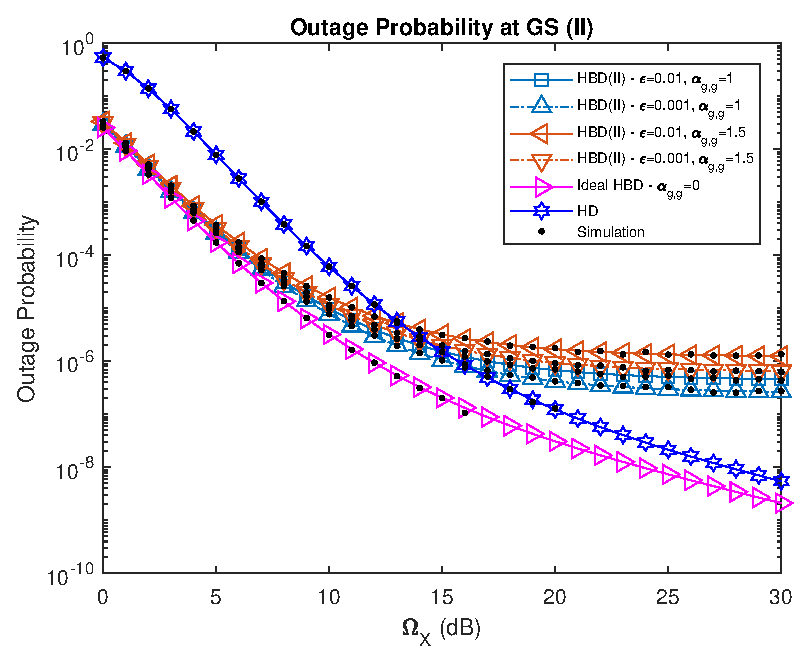
\includegraphics [width=0.45\columnwidth]{chap3_fig/fixed_pout_gs.eps}
\label{fig:interference_management_HBD_ACS_fixed_pout_gs}}
\hfil
\subfloat[Finite SNR diversity gain comparison at GS]{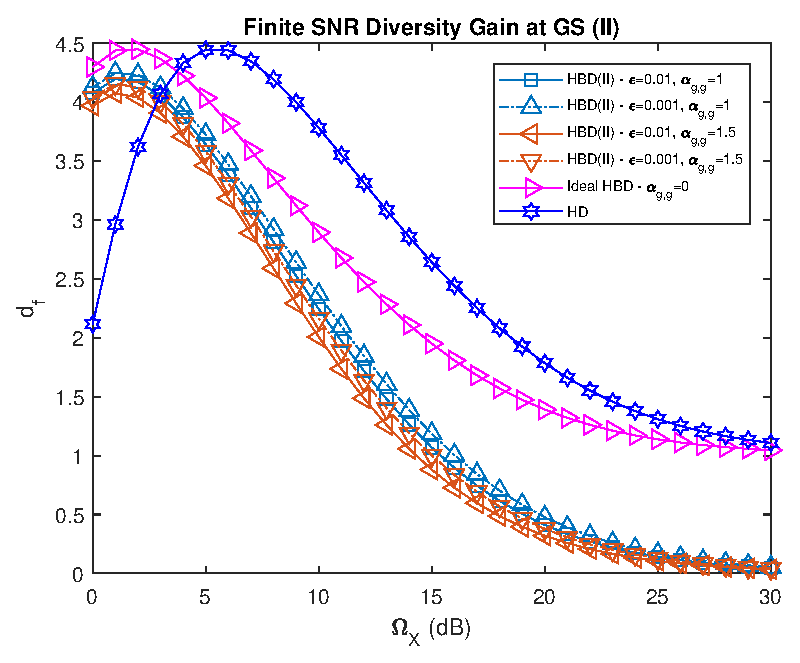
\includegraphics [width=0.45\columnwidth]{chap3_fig/fixed_df_gs.eps}
\label{fig:interference_management_HBD_ACS_fixed_df_gs}}
\caption{Outage probability and finite SNR diversity gain at GS (II detector) for phase noise strength $\gamma_{\phi}^2=-130$ dBm.}
\label{fig:interference_management_HBD_ACS_gs_outage_diversity_gain}
%\vspace{-0.7cm}
\end{figure*}

The HBD outage probability at GS is shown in Fig. \ref{fig:interference_management_HBD_ACS_fixed_pout_gs}. The ideal HBD and the HD outage probability are also plotted in Fig. \ref{fig:interference_management_HBD_ACS_fixed_pout_gs} as a benchmark comparison. From Fig. \ref{fig:interference_management_HBD_ACS_fixed_pout_gs}, it can be seen that $Pr\big(\mathcal{O}_{gs}^{HBD}\big)$ is close to the ideal HBD case, i.e., no interference, at low-to-moderate average received power ($\Omega_X$) and vice-versa. As expected, $Pr\big(\mathcal{O}_{gs}^{HBD}\big)$ is higher as SI channel estimation error ($\epsilon$) is increased. In addition, increasing the strength of the residual SI ($\alpha_{g,g}$) degrades the outage performance more than \textcolor{black}{that obtained with} the increase in $\epsilon$ since a larger $\alpha_{g,g}$ corresponds to a higher average residual SI power, with phase noise ($\gamma^2_{\phi}$) scaled accordingly. In fact, $Pr\big(\mathcal{O}_{gs}^{HBD}\big)$ approaches the ideal HBD case when $\alpha_{g,g}=1, \epsilon=0.001$ at low $\Omega_X$ in Fig. \ref{fig:interference_management_HBD_ACS_fixed_pout_gs}. Hence, sufficient SI mitigation is needed in order for the FD-enabled GS to outperform the HD-enabled GS. 

The finite SNR diversity gain at GS is shown in Fig. \ref{fig:interference_management_HBD_ACS_fixed_df_gs}, where it can be seen that $d_{f,gs}^{HBD}$ peaks at $\Omega_X=2$ dB while $d_{f,gs}^{HD}$ peaks at $\Omega_X=6$ dB. \footnote{Higher diversity gain does not mean lower outage probability and vice-versa. To get a parametric representation for outage probability from diversity gain and SNR, the array gain, coding gain, or SNR offset, needs to be factored as shown in \cite{ordonez2012array} and the references therein. Similar analysis is needed from the interference-limited receiver's perspective to quantify the SNR offsets for different protocols at a given interference level, and it is left as a future extension of the current chapter.} Additionally, (\ref{interference_management_HBD_ACS_asymp_df_fixed_GS}) and (\ref{interference_management_HBD_ACS_lim_df_fixed_hd}) are also confirmed in Fig. \ref{fig:interference_management_HBD_ACS_fixed_df_gs} as $\Omega_X \to \infty$ and is also corroborated in Fig. \ref{fig:interference_management_HBD_ACS_fixed_pout_gs}, where the slope of the outage probability curves become constant as $\Omega_X \to \infty$. In other words, the FD-enabled GS becomes interference-limited at high $\Omega_X$. Interestingly, in the absence of interference at the FD-enabled GS, $d_{f,gs}^{HBD} \to 1$ as $\Omega_X \to \infty$ since only SNR needs to be considered at GS. From Fig. \ref{fig:interference_management_HBD_ACS_gs_outage_diversity_gain}, residual SI is the performance limiting factor for the FD-enabled GS. Therefore, it is important to sufficiently mitigate SI at each of the cascaded stages in Fig. \ref{fig:interference_management_HBD_ACS_1} in order to keep the strength of the residual SI low \textcolor{black}{in practical realizations of the FD-enabled GS}.

\begin{figure*}[]
%\vspace{-0.5cm}
\centering
\subfloat[Outage probability comparison at AS-2]{\includegraphics [width=0.45\columnwidth]{chap3_fig/fixed_pout_as2.eps}
\label{fig:interference_management_HBD_ACS_fixed_pout_as2}}
\hfil
\subfloat[Finite SNR diversity gain comparison at AS-2]{\includegraphics [width=0.45\columnwidth]{chap3_fig/fixed_df_as2.eps}
\label{fig:interference_management_HBD_ACS_fixed_df_as2}}
\caption{Outage probability and finite SNR diversity gain at AS-2 (II and SIC detectors) for $\alpha_{g,2}=1$, i.e., link between GS and AS-2 has same distance as the reference link ($d_{1,g}$).}
%\vspace{-1cm}
\label{interference_management_HBD_ACS_fig_sim}
\end{figure*}

\subsubsection{Impact of Interference at AS-2}

\begin{observation}
\emph{\emph{The II and SIC detectors achieve lower outage probability and higher diversity gain than HD-mode at low SNR regimes and are interference-limited at high SNR regimes. For the SIC detector, strong interference at low SNR regime enables easy removal of the interfering signal.}
}\end{observation}

The HBD outage probabilities at AS-2 for both II and SIC detectors are shown in Fig. \ref{fig:interference_management_HBD_ACS_fixed_pout_as2}. It can be seen that the II detector at AS-2 outperforms the HD mode at low-to-moderate $\Omega_X$ when inter-AS interference ($\alpha_{1,2}$) is weak. The trend in Fig. \ref{fig:interference_management_HBD_ACS_fixed_pout_as2} also suggests that the further reduction in $\alpha_{1,2}$ will enable the II detector at AS-2 to attain the ideal HBD outage performance for moderate $\Omega_X$, which is expected since $\alpha_{1,2}\to 0$ corresponds to diminishing levels of interference at AS-2. 

The SIC detector performs better than the HD mode at the low-to-moderate $\Omega_X$ when interference is strong, e.g., $\alpha_{1,2}=10$, since stage 1 of the SIC detector is more likely to detect and subtract $x_1[t]$. The resultant signal at stage 2 of the SIC detector is thus almost interference-free. As $\alpha_{1,2}$ increases, the SIC detector performance approaches that of the ideal HBD case due to the near perfect cancellation of interference in the first stage. When $\Omega_X>10$ dB for $\alpha_{1,2}\in\{5,10\}$, an error floor is present which verifies Corollary \ref{interference_management_HBD_ACS_coro_asymp_df_fixed_AS2}. Similar error floor observations are also made for the II detector and it indicates that the II and SIC detectors become interference-limited at high $\Omega_X$. From a practical perspective, the trend in Fig. \ref{fig:interference_management_HBD_ACS_fixed_pout_as2} shows that the II detector is well suited for en route scenarios with less congested flight routes such as those over sparsely populated or oceanic regions since the II detector experiences weak interference due to path loss as a result of large inter-aircraft or aircraft to GS distance. On the other hand, the SIC detector is suitable for use in congested airspace scenarios such as the landing or even continental en route scenarios as interference from nearby aircrafts can be effectively removed. Although HD-ACS has superior outage performance compared to the II and SIC detectors at high $\Omega_X$, the interference-limited HBD detectors can meet typical QoS requirements, e.g., frame error rate $\leq 10^{-3}$.

The finite SNR diversity gains, $d_{f,2}^{HBD(II)}$ and $d_{f,2}^{HBD(SIC)}$, at AS-2 are shown in Fig. \ref{fig:interference_management_HBD_ACS_fixed_df_as2}. A trend similar to what was seen in Fig. \ref{fig:interference_management_HBD_ACS_fixed_df_gs} can be found in Fig. \ref{fig:interference_management_HBD_ACS_fixed_df_as2}, with $d_{f,2}^{HBD(II)}$ and $d_{f,2}^{HBD(SIC)}$ peaking at $\Omega_X=2$ dB, and $d_{f,2}^{HD}$ peaking at $\Omega_X=6$ dB. As expected, reducing $\alpha_{1,2}$ causes $d_{f,2}^{HBD(II)}$ to perform close to the ideal HBD case at low $\Omega_X$. Fig. \ref{fig:interference_management_HBD_ACS_fixed_df_as2} also confirms (\ref{interference_management_HBD_ACS_asymp_df_fixed_AS2}) for both the II and SIC detectors. It is clear that the SIC detector can attain an outage probability decay rate that is similar to the ideal HBD case when $\Omega_X\leq5$ dB. Further increasing $\alpha_{1,2}$ will enable $d_{f,2}^{HBD(SIC)}$ to be almost identical to the ideal HBD case at $\Omega_X\leq5$ dB since the system becomes noise-limited rather than interference-limited. The trends in Fig. \ref{fig:interference_management_HBD_ACS_fixed_df_as2} are also reflected in Fig. \ref{fig:interference_management_HBD_ACS_fixed_pout_as2} since the slope of the outage probability curves behave as indicated in (\ref{interference_management_HBD_ACS_asymp_df_fixed_AS2}) and (\ref{interference_management_HBD_ACS_lim_df_fixed_hd}) as $\Omega_X \to \infty$.

\begin{figure*}[]
\centering
\subfloat[System level outage probability]{\includegraphics [width=0.45\columnwidth]{chap3_fig/fixed_pout_sys.eps}
\label{fig:interference_management_HBD_ACS_fixed_pout_sys}}
\hfil
\subfloat[System level finite SNR diversity gain]{\includegraphics [width=0.45\columnwidth]{chap3_fig/fixed_df_sys.eps}
\label{fig:interference_management_HBD_ACS_fixed_df_sys}}
\caption{System level outage probability and finite SNR diversity gain (II and SIC detectors) for $\alpha_{g,2}=1$,$\alpha_{g,g}=1$,$\gamma_{\phi}^2=-130$ dBm, $\epsilon\in\{0.01, 0.001\}$.}
%\vspace{-1cm}
\label{interference_management_HBD_ACS_fig_sim}
\end{figure*}

\subsubsection{Impact of Interference at System Level}

\begin{observation}
\emph{\emph{The system level performance of the HBD-ACS is constrained by inter-AS interference. When the II detector is considered, weak inter-AS interference enables near-ideal system level performance. Likewise for the SIC detector when strong inter-AS interference is present. If the SI suppression level is lower, then it is possible for the GS to be the bottleneck.}
}\end{observation}

Fig. \ref{fig:interference_management_HBD_ACS_fixed_pout_sys} and Fig. \ref{fig:interference_management_HBD_ACS_fixed_df_sys} respectively shows the outage probability and finite SNR diversity gain at the system level. Through numerical analysis, we observed that $P_{out,system}^{HBD(II)}$ is dominated by the II detector at AS-2 for $\alpha_{1,2} \in \{0.1, 0.5\}$ and $0 \text{ dB} \leq \Omega_X \leq 30 \text{ dB}$, i.e., $Pr\big(\mathcal{O}_{gs}^{HBD}\big)<Pr\big(\mathcal{O}_{2}^{HBD(II)}\big)$ because inter-AS interference at AS-2 is stronger than the residual SI experienced at GS. Thus, although not shown in the figure, increasing $\alpha_{g,g}$ or $\epsilon$ does not affect $P_{out,system}^{HBD(II)}$ unless inter-AS interference is decreased. It can also be observed from Fig. \ref{fig:interference_management_HBD_ACS_fixed_pout_sys} that $P_{out,system}^{HBD(II)} \leq P_{out,system}^{HD}$ when $\Omega_X\leq4$ dB, $\alpha_{1,2}=0.5$. When $\alpha_{1,2}=0.1$, $P_{out,system}^{HBD(II)} \leq P_{out,system}^{HD}$ for $\Omega_X\leq11$ dB. In fact, $P_{out,system}^{HBD(II)}$ approaches that of the ideal HBD case when $\alpha_{1,2}$ is decreased due to the near absence of inter-AS interference at the II detector and it also explains the trend seen in Fig. \ref{fig:interference_management_HBD_ACS_fixed_df_sys} where it can be seen that $d_{f,system}^{HBD(II)}$ approaches that of the ideal HBD case when $\alpha_{1,2}$ is decreased. In other words, the decay of $P_{out,system}^{HBD(II)}$ approaches that of the ideal HBD case when inter-AS interference weakens, as reflected in Fig. \ref{fig:interference_management_HBD_ACS_fixed_df_sys}, for $\Omega_X \leq 5$ dB. Therefore, when an II detector is used at AS-2, the inter-AS interference is the limiting factor for both $P_{out,system}^{HBD(II)}$ and $d_{f,system}^{HBD(II)}$.

When AS-2 adopts an SIC detector, $P_{out,system}^{HBD(SIC)}$ is dominated by GS when $\Omega_X\leq4$ dB and $\alpha_{1,2}=5$. Similar trends for the SIC detector are also seen in Fig. \ref{fig:interference_management_HBD_ACS_fixed_df_sys} for $\Omega_X \leq 5$ dB. When $\Omega_X>4$ dB, $P_{out,system}^{HBD(SIC)}$ is dominated by AS-2 and it can be explained from the perspective of the two-stage SIC detector at AS-2. When $\alpha_{1,2}=5$, $x_1[t]$ is five times stronger than the SOI from GS ($x_{gs}[t]$). In addition, at stage 1 of the SIC detector, noise power ($\sigma^2_{2}$) is stronger than $x_{gs}[t]$ when $\Omega_X\leq4$ dB. Thus, the SIC detector is more likely to detect and cancel $x_1[t]$ which results in $Pr\big(\mathcal{O}_{gs}^{HBD}\big)>Pr\big(\mathcal{O}_{2}^{HBD(SIC)}\big)$ due to residual SI at GS. When $\Omega_X>4$ dB, $\sigma_2^2$ will be weaker than $x_{gs}[t]$ at stage 1 of the SIC detector. Consequently, the SIC detector is less likely to detect and cancel $x_1[t]$, leading to $Pr\big(\mathcal{O}_{gs}^{HBD}\big)<Pr\big(\mathcal{O}_{2}^{HBD(SIC)}\big)$. When $\alpha_{1,2}=10$, $P_{out,system}^{HBD(SIC)}$ is dominated by GS for $\Omega_X \leq 10$ dB due to stronger interference at AS-2, with $P_{out,system}^{HBD(SIC)}$ close to that of the ideal HBD case. Further increasing $\alpha_{1,2}$ enables $P_{out,system}^{HBD(SIC)}$ to reach near-ideal HBD performance for a wider $\Omega_X$ range due to the increased likelihood of successfully detecting and canceling $x_1[t]$, thus explaining the trend in Fig. \ref{fig:interference_management_HBD_ACS_fixed_df_sys}. Hence, the strength of the interference from AS-1 ($\alpha_{1,2}$) is the main limiting factor for both $P_{out,system}^{HBD(SIC)}$ and $d_{f,system}^{HBD(SIC)}$ when a SIC detector is used at AS-2. 

%The finite SNR diversity gain analysis has indicated that inter-AS interference is the performance limiting factor for both II and SIC detectors at low $\Omega_X$, which would not have been revealed through asymptotic diversity gain analysis. 

From Fig. \ref{fig:interference_management_HBD_ACS_fixed_pout_sys} and Fig. \ref{fig:interference_management_HBD_ACS_fixed_df_sys}, the outage and finite SNR diversity gain analysis has highlighted the feasibility of HBD-ACS over legacy HD-ACS in weak and strong interference scenarios through the II and SIC detectors, respectively. For instance, weak and strong interference scenarios could involve en route flights over sparely and densely populated airspace, respectively. From \textcolor{black}{the perspective of implementing an actual HBD system}, the proposed HBD-ACS has better reliability over HD-ACS while providing more throughput than legacy HD systems. 

\subsection{Finite SNR DMT Analysis}

\subsubsection{Impact of Residual SI at GS}

\begin{observation}
\emph{\emph{The FD-enabled GS achieves non-zero diversity gain for a larger range of multiplexing gains compared to the HD GS.}
}\end{observation}

\begin{figure*}[]
\centering
\subfloat[GS (II detector).]{\includegraphics [width=0.45\columnwidth]{chap3_fig/var_df_gs.eps}
\label{fig:interference_management_HBD_ACS_var_df_gs}}
\hfil
\subfloat[AS-2 (II and SIC detector).]{\includegraphics [width=0.45\columnwidth]{chap3_fig/var_df_as2.eps}
\label{fig:interference_management_HBD_ACS_var_df_as2}}
\caption{Finite SNR DMT for $\alpha_{g,2}=1, \gamma_{\phi}^2=-130 \text{ dBm}, \Omega_X=10 \text{ dB}$.}
%\vspace{-1cm}
\label{interference_management_HBD_ACS_fig_sim}
\end{figure*}

Fig. \ref{fig:interference_management_HBD_ACS_var_df_gs} shows the finite SNR diversity gain at GS, where it is evident that the stronger residual SI due to SI channel estimation error ($\epsilon$) or phase noise ($\gamma_{\phi}^2$) reduces $d_{f,gs}^{HBD*}$. Increasing the strength of the residual SI ($\alpha_{g,g}$) affects $d_{f,gs}^{HBD*}$ more than increasing the SI channel estimation error ($\epsilon$) since the effect of phase noise ($\gamma_{\phi}^2$) on the residual SI is amplified. From the outage probability perspective, increasing residual SI results in a slower decay rate of the outage probability, which lowers $d_{f,gs}^{HBD*}$. However, it does not imply that outage probability is better when a higher maximum value for $d_{f,gs}^{HBD*}$ is attained. Nonetheless, the range of $r_f$ for which $d_{f,gs}^{HBD*}\geq d_{f,gs}^{HD*}$ increases when the strength of the residual SI ($\alpha_{g,g}$) decreases and vice versa. Therefore, FD-enabled GS can experience improved DMT as residual SI decreases, which is evident in Fig. \ref{fig:interference_management_HBD_ACS_var_df_gs} for $\alpha_{g,g}=1$. Although $d_{f,gs}^{HBD*}$ is limited by residual SI, the importance of proper SI mitigation is again emphasized since it is still feasible for GS to be FD-enabled if operating at a higher $r_f$ is the objective of an ACS.

\subsubsection{Impact of Interference at AS-2}

\begin{observation}
\emph{\emph{At low multiplexing gains, the II and SIC detectors have lower finite SNR diversity gain. In contrast, at high multiplexing gains, the II and SIC detectors achieve near-ideal finite SNR diversity gain under weak and strong inter-AS interference, respectively.}
}\end{observation}

Fig. \ref{fig:interference_management_HBD_ACS_var_df_as2} shows the finite SNR diversity gain at AS-2. The trends seen in Fig. \ref{fig:interference_management_HBD_ACS_var_df_as2} are similar to what was seen in \cite[Fig. 4]{narasimhan2006finite}, with lower $d_{f,2}^{HBD(i)*}, i \in \{II,SIC\}$ and $d_{f,2}^{HD*}$ observed as $r_f \to 0$. It has been pointed out by Narasimhan \cite{narasimhan2006finite} and Shin et al. \cite{shin2008diversity} that Rician fading outage probability curves are influenced by Rician $K$ factors. In particular, increasing the Rician $K$ factor causes the slope of outage probability curves to become steeper \cite[Fig. 2]{shin2008diversity}. From a finite SNR DMT perspective, $r_f \to 0$ causes $K_{X_{gs}}$ to have less impact on the outage performance at AS-2. 

On the other hand, Fig. \ref{fig:interference_management_HBD_ACS_var_df_as2} also suggests that the II and SIC detectors are able to provide better reliability at higher multiplexing gains compare to HD systems. At high multiplexing gains, if the inter-AS interference reduces, then $d_{f,2}^{HBD(II)*} \geq d_{f,2}^{HD*}$. On the other hand, at low multiplexing gains, $d_{f,2}^{HBD(II)*} < d_{f,2}^{HD*}$ even at low inter-AS interference. In fact, $d_{f,2}^{HBD(II)*}$ approaches that of the ideal HBD case as $\alpha_{1,2} \to 0$ since the signal at the II detector is almost interference-free. As a consequence, the resultant outage probability decay rate becomes similar to that of the ideal HBD case. When the SIC detector is adopted at AS-2, $d_{f,2}^{HBD(SIC)*} \geq d_{f,2}^{HD*}$ as inter-AS interference increases (for example, refer to $d_{f,2}^{HBD(SIC)*}$ at $\alpha_{1,2} = 14.3$ in Fig. \ref{fig:interference_management_HBD_ACS_var_df_as2}). As $\alpha_{1,2}\to\infty$, it becomes easier to detect and remove $x_1[t]$ at the two-stage SIC detector. When coupled with the lower threshold requirement of the SIC detector, as compared to HD systems, the SIC detector can potentially achieve superior diversity gains over HD systems in strong interference scenarios. Moreover, at large values of $\alpha_{1,2}$, if the multiplexing gain is high, the achievable $d_{f,2}^{HBD(SIC)*}$ matches the ideal HBD case. As shown in Fig. \ref{fig:interference_management_HBD_ACS_var_df_as2}, at low multiplexing gain, the achievable $d_{f,2}^{HBD(SIC)*}$ is close to that of the ideal HBD case. Therefore, the II and SIC detectors provides better reliability at higher multiplexing gains compared to HD-ACS in the presence of weak and strong interference, respectively. However, at low multiplexing gains, HD-ACS exhibited better reliability than the II and SIC detectors.

\begin{figure} []
\centering
%\vspace{-1cm}
\includegraphics [width=0.45\columnwidth]{chap3_fig/var_df_sys.eps} 
%\vspace{-0.5cm}
\caption{System level finite SNR DMT (II and SIC detectors) for $\alpha_{g,2}=1$, $\alpha_{g,g}=1$, $\gamma_{\phi}^2=-130 \text{ dBm}$, $\Omega_X=10 \text{ dB}$.}
%\vspace{-0.5cm}
\label{fig:interference_management_HBD_ACS_var_df_sys}
\end{figure}

\subsubsection{Impact of Interference at System Level}

\begin{observation}
\emph{\emph{At high multiplexing gains, the HBD-ACS achieves better finite SNR diversity gain at the system level than the HD-ACS and is also constrained by inter-AS interference and residual SI.}
}\end{observation}

Fig. \ref{fig:interference_management_HBD_ACS_var_df_sys} shows the system level finite SNR diversity gain for HBD-ACS ($d_{f,system}^{\beta*}$) and HD-ACS ($d_{f,system}^{HD*}$) for $\beta \in \{HBD(II), HBD(SIC)\}$. From Fig. \ref{fig:interference_management_HBD_ACS_var_df_sys}, it is evident that $d_{f,system}^{HBD(II)*} > d_{f,system}^{HD*}$ and $d_{f,system}^{HBD(SIC)*} > d_{f,system}^{HD*}$ as $r_f$ increases, and it enables an HBD-ACS to provide better reliability at higher multiplexing gain than HD-ACS since HBD-ACS requires a lower operating threshold than existing HD-ACS at both GS and AS-2. However, the degree of improvement that HBD-ACS has over HD-ACS is constrained by the strength of interference experienced at GS and AS-2 in the HBD-ACS.

When the II detector is adopted at AS-2 for weak interference scenarios, $d_{f,gs}^{HBD*} > d_{f,2}^{HBD(II)*}$ for $\alpha_{1,2}=0.1$. Reducing the strength of the inter-AS interference ($\alpha_{1,2}=0.01$) causes $d_{f,2}^{HBD(II)*} > d_{f,gs}^{HBD*}$, with lower SI channel estimation error ($\epsilon $) corresponding to higher $d_{f,system}^{HBD(II)*}$. In the presence of strong interference at AS-2 ($\alpha_{1,2}=100$), adopting the SIC detector at AS-2 results in $d_{f,2}^{HBD(SIC)*} > d_{f,gs}^{HBD*}$. However, when interference from AS-1 is not as strong, e.g., $\alpha_{1,2} \in \{14.3, 15\}$, then $d_{f,gs}^{HBD*} > d_{f,2}^{HBD(SIC)*}$. From Fig. \ref{fig:interference_management_HBD_ACS_var_df_sys}, the reliability of the HBD-ACS depends on the inter-AS interference at AS-2 for both II and SIC detectors and residual SI at GS. Furthermore, it is possible for the proposed HBD-ACS to attain finite SNR DMT curves that are identical to the ideal HBD case at sufficiently low residual SI.

From Fig. \ref{fig:interference_management_HBD_ACS_var_df_sys}, the trends show that the proposed HBD-ACS is a viable alternative to legacy HD-ACS in weak and strong interference scenarios. In particular, the proposed HBD-ACS can operate at a higher multiplexing gain than legacy HD-ACS, thus offering better throughput and reliability compared to the latter.

%%%%%%%%%%%%%%%%%%%%%%%%%%%%%%%%%%%%%%%%%%%%%%%%%%%%%%%%%%%%%%%%%%%%%%%%%%%%%%%%%%%%%%%%%%%%%%%%%%%%%%%%%%%%%%%%%%%%%%%%%%%%%%%%%%%%%%%%%

% Section: Conclusion
\section{Chapter Summary}
An HBD-ACS consisting of an FD-enabled GS and two HD ASs simultaneously communicating on the same spectrum is proposed to improve spectrum utilization. To investigate the impact of interference on the proposed HBD-ACS, closed-form outage probability and finite SNR diversity gain expressions are presented in this chapter for a SIC detector over Rician fading aeronautical channels. Through outage and finite SNR diversity gain analysis, it is established that residual SI is the main limiting factor at the FD-enabled GS. Therefore, the need for sufficient SI mitigation must be properly addressed in a HBD-ACS. At AS-2, inter-AS interference is the main limiting factor for both II and SIC detectors. At the system level, the proposed HBD-ACS is found to be very suitable for weak and strong interference scenarios for the II and SIC detectors, respectively. The proposed HBD-ACS is also able to achieve superior outage performance and better diversity gains at low-to-moderate SNRs compared to existing HD-ACS for both weak and strong interference scenarios. Finite SNR DMT analysis has also revealed that HBD-ACS can achieve interference-free diversity gain if residual SI is sufficiently suppressed, enabling HBD-ACS to be more reliable than HD-ACS at higher multiplexing gains while operating at low SNR ranges.

As this chapter focuses on HBD systems in aeronautical communications for weak and strong interference scenarios, the JD approach is investigated in the next chapter for moderate interference environments in UAV communications.




%---------------------------------------------------------------------------------
\chapter{Interference Management Through Joint Detection for Hybrid-Duplex UAV Communications}
\label{chap:JD_HBD_UCS}
%---------------------------------------------------------------------------------
\section{Introduction}
%\subsection{Motivation and Related Literature}
In Chapter \ref{chap:interference_management_HBD_ACS}, HBD-ACSs are studied as a potential solution to address spectrum scarcity in MAV communications as a result of air traffic growth in the near future. Apart from MAV communications, air traffic growth for UAVs is also expected to grow rapidly in the years to come. Despite the potential benefits of multi-UAV networks, many challenges remain. One notable instance is the allocation of L-band and C-band spectrum by the ITU for UAV communications, e.g., for CNPC applications \cite{matolak2017air_suburban}. However, there is limited available spectrum for UAV communications as many other systems, e.g., aeronautical communication systems, also operate on L-band and C-band \cite{matolak2017air_suburban}. Therefore, spectrum scarcity in UAV communications is an issue that must be addressed in due time. 

To this end, an HBD-UCS has been studied as a viable alternative to improve spectrum utilization with minimal disruptions \cite{tan2018ricianShad}. With suitable SI mitigation architectures, HBD systems enable HD and FD-enabled nodes to operate concurrently on the same spectrum, leading to improved spectrum utilization. While opting for an FD-UCS, i.e., UAVs and GSs operating in FD mode, results in better spectrum utilization over the HBD paradigm, constraints imposed on the size, weight, and power requirements of UAVs may cause FD transceiver designs to be infeasible.\footnote{The work in this chapter has been published in \cite{tan2018joint}.} Therefore, opting for an HBD-UCS allows spectrum utilization to be addressed while retaining existing HD-UCS, with related applications seen in aeronautical communication systems \cite{ernest2018performance,ernest2019outage}.

% Research Problem 1: Inter-UAV interference
Apart from SI, inter-UAV interference is also present at the HD UAVs in the HBD-UCS. Regarding this, interference management strategies, such as the II, SIC, or the JD strategies, can be adopted to mitigate inter-UAV interference. The II approach regards interference as noise and is optimal in weak interference scenarios \cite{annapureddy2009gaussian,zahavi2017cooperation} while the SIC approach, which first removes interference before detecting the SOI, is effective in strong interference scenarios \cite{qu2014understanding,weber2007transmission}. On the other hand, the JD approach jointly decodes the SOI and interference at the receiver, and is optimal when strong interference is present albeit at the cost of high computational complexity \cite{zhou2015mac,shubhi2017joint}. In \cite{ernest2018performance} and \cite{ernest2019outage}, outage probability analysis of HBD aeronautical communication systems showed that the II and the SIC strategies are interference-limited at high SNR regimes and are effective in weak and strong interference scenarios, respectively. However, in the context of UAV communications, suitable interference management strategies to handle the different levels of inter-UAV interference in multi-UAV systems have still yet not been identified.

Another issue in HBD-UCS is the need to concurrently meet QoS requirements for both CNPC links and non-CNPC links as a result of simultaneous communications over a common spectrum \footnote{To enable the sharing of the spectrum for CNPC and non-CNPC links with a joint detector, the block length of the codes used, e.g., LDPC codes, should be the same \cite{sharifi2016ldpc}.}. To safely operate multi-UAV systems, CNPC links have high reliability and low data rate requirements \cite{zeng2016wireless}. On the other hand, non-CNPC links, i.e., data links, have higher data rate requirements than CNPC links, which is dependent on the task at hand \cite{zeng2016wireless}. As the QoS requirements of both CNPC and non-CNPC links must be concurrently satisfied in the HBD-UCS, the extent of reliability tradeoffs for higher transmission rates in the presence of inter-UAV interference is not yet known. More importantly, it still remains to be seen if the HBD-UCS can better meet the necessary QoS requirements compared to existing HD-UCS.

To this end, the finite SNR diversity gain and finite SNR DMT of the HBD-UCS can be analyzed. The finite SNR diversity gain and finite SNR DMT describe outage probability decay rate (reliability) at a particular SNR \cite{shin2008diversity}, with multiplexing gain (data rate) considered in the latter \cite{narasimhan2006finite}. Such analysis reveals the outage probability behavior of the HBD-UCS at low SNR regimes, which is lost at asymptotic SNRs \cite{shin2008diversity}. A corresponding MGR of the HBD-UCS can also be determined \cite{karmakar2012generalized} to identify the multiplexing gains of the interfering and desired transmitters that achieves non-zero diversity gains. Through diversity gain and MGR analysis, the supported QoS range of the HBD-UCS, along with the necessary conditions to achieve non-zero diversity gains, e.g., inter-UAV interference levels and data rates, for various interference management strategies can be identified.

%%%%%%%%%%%%%%%%%%%%%%%%%%%%%%%%%%%%%%%%%%%%%%%%%%%%%%%%%%%%%%%%%%%%%%%%%%%%%%%%%%%%%%%%%%%%%%%%%%%%%%%%%%%%%%%%%%%%%%%%%%%%%%%%%%%%%%%%%
% Section 2 : System Model
\section{System Model}
\begin{figure} [tpb]
\centering
\vspace{-2cm}
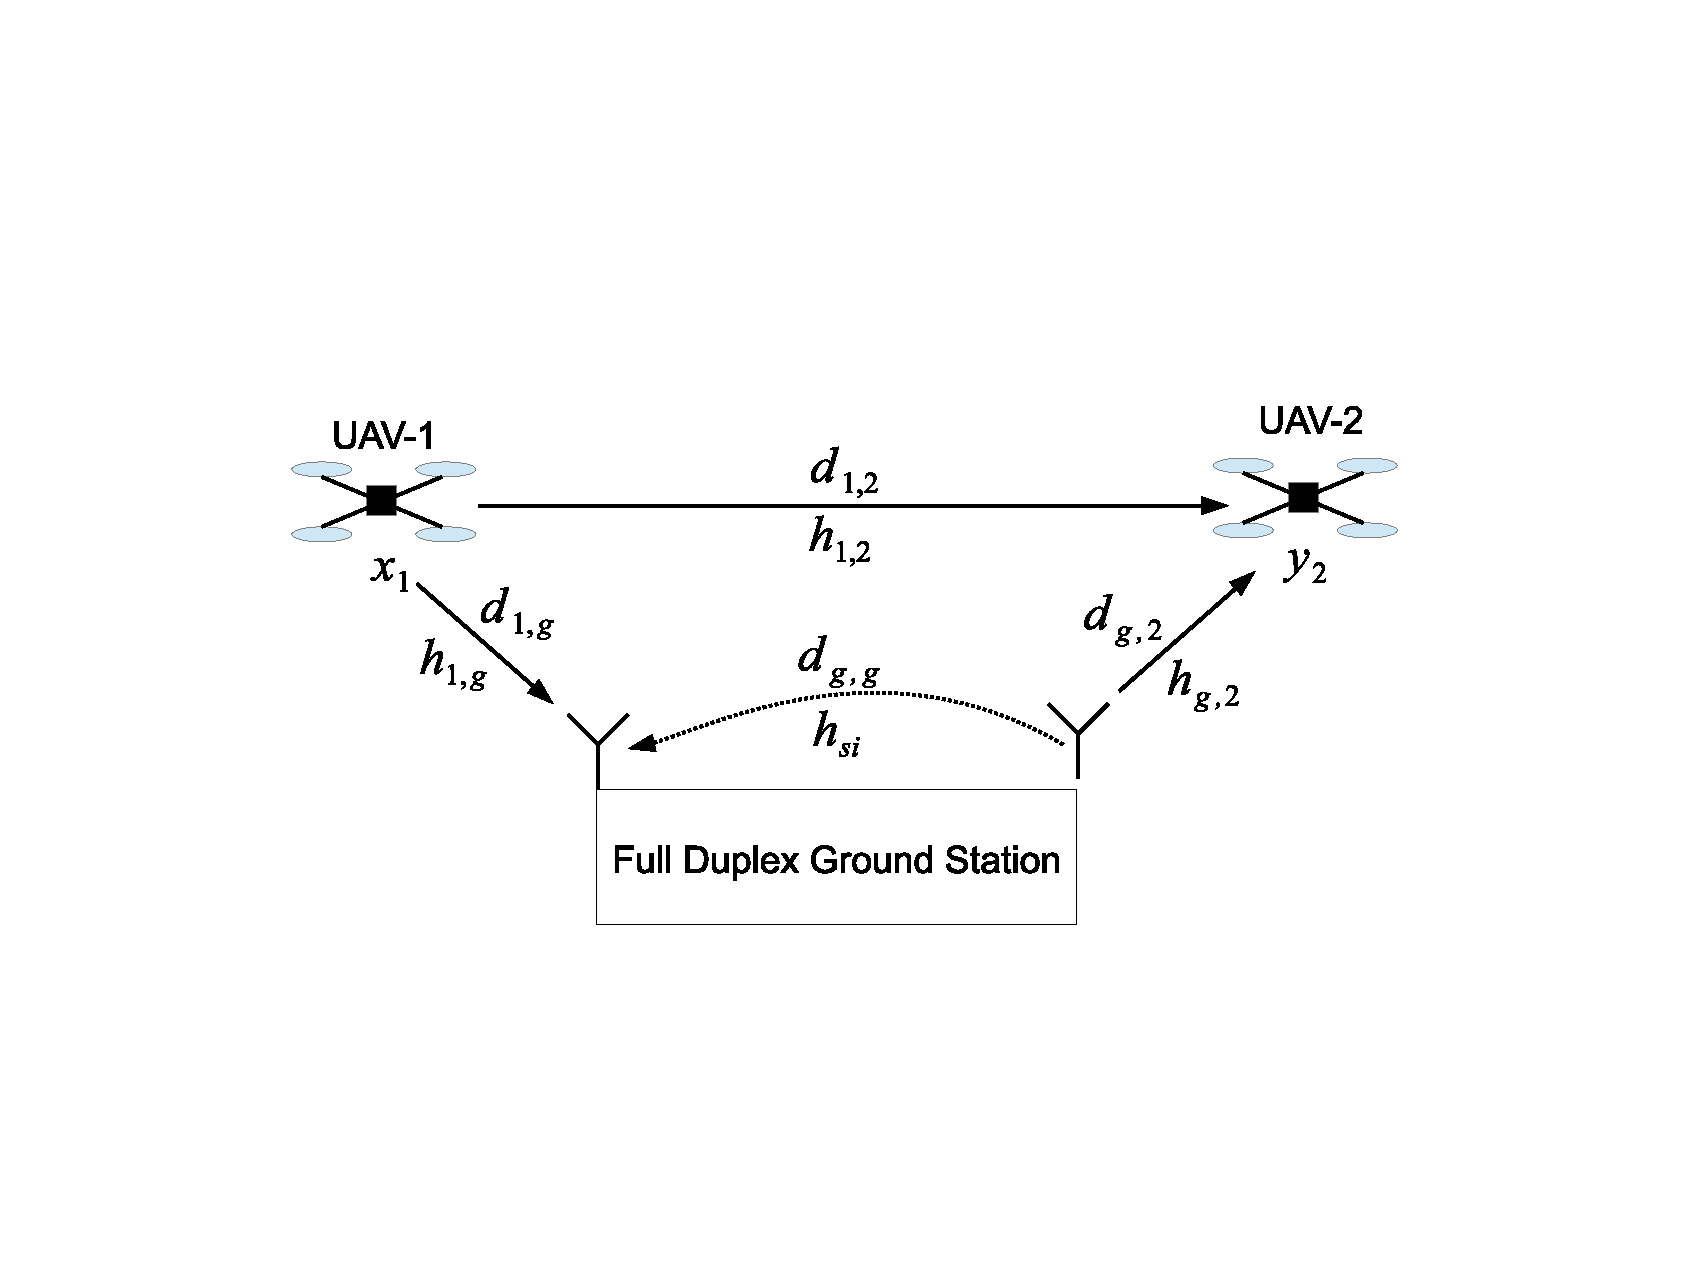
\includegraphics [width=0.8\columnwidth]{chap4_fig/block_diagram.eps} 
\vspace{-2.2cm}
\caption{Unmanned Aerial Vehicle 1 (UAV-1) and Unmanned Aerial Vehicle 2 (UAV-2) operating in HD mode while communicating with the FD GS.}
%\vspace{-0.5cm}
\label{fig:JD_HBD_UCS_1}
\end{figure}

Fig. \ref{fig:JD_HBD_UCS_1} shows the proposed HBD-UCS for UAV communications in a suburban environment between an FD-enabled GS node and two HD UAVs. \textcolor{black}{\footnote{\textcolor{black}{The present chapter can be extended to consider an arbitrary number of uplink and downlink UAVs. To enable the modeling and analysis of such a multi-UAV network, the signal model at the GS and downlink UAVs will need to be modified. Furthermore, stochastic geometry tools, i.e., the BPP model, will need to be employed to accurately model UAV deployment. These issues are addressed in Chapter \ref{chap:HBD_multi_UAV}, where new signal models that considers the BPP model are proposed for an HBD multi-UAV network.}}} In particular, Unmanned Aerial Vehicle 1 (UAV-1) transmits non-CNPC data to the GS while Unmanned Aerial Vehicle 2 (UAV-2) concurrently receives CNPC data from the GS on the same spectrum, e.g., L-band. Two antennas, one for transmission and another for reception of signals, with a shared local oscillator are assumed at the FD-enabled GS. Also, the Doppler effect as a result of UAV mobility is assumed to be compensated. Clearly, spectrum utilization is improved at the expense of introducing SI and inter-UAV interference at the FD-enabled GS and UAV-2, respectively. To enable realistic modeling of the suburban environment, Rician fading is assumed on all UAV communication channels \cite{matolak2017air_suburban}. Additionally, the SI signal is assumed to undergo passive SI mitigation before active SI mitigation at the FD-enabled GS. Thus, we consider only residual SI at the FD-enabled GS, with the SI link ($h_{si}$) modeled as a Rician fading channel to account for passive and active SI mitigation \cite{ahmed2015all}. A summary of important notations is also given in Table \ref{table:JD_HBD_UCS_summary_impt_notations}.

\subsection{Ground Station}
At the FD-enabled GS, let $x_{gs}[t]$ and $x_1[t]$ be the transmitted signals from GS and UAV-1, respectively, where the SOI and the SI signal are $x_1[t]$ and $x_{si}[t]=x_{gs}[t]$, respectively. Additionally, let $h_{1,g}[t]$ be the channel between UAV-1 and GS, and $h_{si}$ be the SI channel gain. Then, the received signal at GS can be written as \cite{sahai2013impact}:
%%%%%%%%%%%%%%%%%%%%%%%%%%%%%%%%%%%%%%%%%%%%%%%%%%%%%%%%%%%%%%%%%%%%%%%%%%%%%%%%%
\begin{eqnarray} \label{JD_HBD_UCS_y_gs}
y_{gs}[t] & = & \sqrt{\Omega_{X}}h_{1,g}[t]x_{1}[t] + \sqrt{\Omega_X\alpha_{g,g}}|h_{si}|\gamma_{\phi}w_{\phi}[t]  + \sqrt{\Omega_X\alpha_{g,g}} |\widetilde{h}_{si}|x_{si}[t] + w_{g}[t],
\end{eqnarray}
%%%%%%%%%%%%%%%%%%%%%%%%%%%%%%%%%%%%%%%%%%%%%%%%%%%%%%%%%%%%%%%%%%%%%%%%%%%%%%%%%
where $\widetilde{h}_{si}$ is the error of the imperfect SI channel gain estimate, defined as $\widetilde{h}_{si}=h_{si}-\widehat{h}_{si}$, and $\widehat{h}_{si}$ is the imperfect estimation of the SI channel gain. To model the worst case residual SI, the channel estimation error ($\widetilde{h}_{si}$) is modeled as a circularly symmetric zero-mean complex Gaussian random variable RV with variance $\epsilon$ \cite{zlatanov2017capacity}.

Additionally, let the AWGN at GS be $w_{g}[t]$, with zero-mean and variance $\sigma_g^2$, and let the phase noise term $w_{\phi}[t]$ follow a Gaussian distribution with zero-mean and unit variance, scaled by the strength of the phase noise $\gamma_{\phi}$ \footnote{The scaling factor $\gamma_{\phi}$ models the jitter present in oscillators due to hardware imperfections \cite{sahai2013impact}} \cite{sahai2013impact}. 


Let the average received signal power of the SOI, normalized with the GS receiver noise variance ($\sigma_g^2$), be $\Omega_{X}$, which is related to the transmit power $P_{t}$ (Watts) and distance $d_{1,g}$ (km) as:
%%%%%%%%%%%%%%%%%%%%%%%%%%%%%%%%%%%%%%%%%%%%%%%%%%%%%%%%%%%%%%%%%%%%%%%%%%%%%%%%%
\begin{eqnarray} \label{JD_HBD_UCS_Omega_x_soi}
\Omega_{X} \propto \frac{P_t}{\left(d_{1,g}\right)^{n}\sigma_g^2},
\end{eqnarray}
%%%%%%%%%%%%%%%%%%%%%%%%%%%%%%%%%%%%%%%%%%%%%%%%%%%%%%%%%%%%%%%%%%%%%%%%%%%%%%%%%
where $n$ is the pathloss exponent. We select the channel between UAV-1 and GS as the reference link, with the average received signal power in the other links expressed relative to the reference link to represent the inter-UAV interference level $\alpha_{i,j}$ as follows:
%%%%%%%%%%%%%%%%%%%%%%%%%%%%%%%%%%%%%%%%%%%%%%%%%%%%%%%%%%%%%%%%%%%%%%%%%%%%%%%%%
\begin{eqnarray} \label{JD_HBD_UCS_alpha_i_j}
\alpha_{i,j} = \bigg(\frac{d_{1,g}}{d_{i,j}}\bigg)^n, i\in\left\{g,1\right\}, j\in\left\{g,2\right\}.
\end{eqnarray}
%%%%%%%%%%%%%%%%%%%%%%%%%%%%%%%%%%%%%%%%%%%%%%%%%%%%%%%%%%%%%%%%%%%%%%%%%%%%%%%%%
From (\ref{JD_HBD_UCS_Omega_x_soi}) and (\ref{JD_HBD_UCS_alpha_i_j}), the average received SI power at GS can be expressed as $\Omega_X\alpha_{g,g}$. 

\subsection{Unmanned Aerial Vehicle 2}

The SOI and the interfering signal at UAV-2 are $x_{gs}[t]$ and $x_1[t]$, respectively. Let $h_{g,2}[t]$ be the channel between GS and UAV-2, and let $h_{1,2}[t]$ be the channel between UAV-1 and UAV-2. Let $w_{2}[t]$ be the AWGN at UAV-2 with zero-mean and variance $\sigma_2^2$. Then, the received signal at UAV-2 can be expressed as:
%%%%%%%%%%%%%%%%%%%%%%%%%%%%%%%%%%%%%%%%%%%%%%%%%%%%%%%%%%%%%%%%%%%%%%%%%%%%%%%%%
\begin{eqnarray} \label{JD_HBD_UCS_y_as2}
y_{2}[t] = \sqrt{\Omega_{X}\alpha_{g,2}}h_{g,2}[t]x_{gs}[t] + \sqrt{\Omega_{X}\alpha_{1,2}}h_{1,2}[t]x_{1}[t] +  w_{2}[t], 
\end{eqnarray}
%%%%%%%%%%%%%%%%%%%%%%%%%%%%%%%%%%%%%%%%%%%%%%%%%%%%%%%%%%%%%%%%%%%%%%%%%%%%%%%%%
where $\Omega_{X}\alpha_{g,2}$ and $\Omega_{X}\alpha_{1,2}$ indicate the average received signal powers of the SOI and interfering signal, respectively. 

As interference is present at UAV-2, we consider three approaches to handle the interference. The first approach is to assume an II detector at UAV-2 by treating $x_1[t]$ as noise, thus effectively ignoring interference. The second approach assumes a two-stage SIC detector at UAV-2 where $x_1[t]$ is detected and removed before $x_{gs}[t]$ is detected \cite{narasimhan2007individual}. The final approach assumes a joint detector where both $x_{gs}[t]$ and $x_1[t]$ are jointly detected \cite{blomer2009transmission}.

\begin{table}[]
\centering
\caption{Summary of Important Notations}
\label{table:JD_HBD_UCS_summary_impt_notations} 
\scalebox{0.8}{
\begin{tabular}{ll}
\hline
\textbf{Notations}		& \textbf{Description}																			\\  \hline \hline
$\Omega_X$						& Average received power																		\\
$\alpha_{i,j}, i\in\left\{g,1\right\}, j\in\left\{g,2\right\}, i \neq j$ & Strength of interference between $i$ and $j$				\\
$\epsilon$						& SI channel estimation error	at the FD-enabled GS					\\
$\gamma_{\phi}^2$			& Strength of phase noise at the FD- enabled GS oscillator	\\
$\sigma_g^2$					& Strength of AWGN at the FD-enabled GS											\\ 
$\sigma_2^2$					& Strength of AWGN at the UAV-2															\\ \hline
\end{tabular}}
\end{table}
%A summary of important notations is also given in Table \ref{table:JD_HBD_UCS_summary_impt_notations}.

%%%%%%%%%%%%%%%%%%%%%%%%%%%%%%%%%%%%%%%%%%%%%%%%%%%%%%%%%%%%%%%%%%%%%%%%%%%%%%%%%%%%%%%%%%%%%%%%%%%%%%%%%%%%%%%%%%%%%%%%%%%%%%%%%%%%%%%%%
% Section 3 : Outage Probability
\section{Outage Probability Derivations} \label{JD_HBD_UCS_subsec_UAV2_JD}
In this section, we derive the closed-form outage probability expression for the joint detector at UAV-2. As inter-UAV interference increases, we show that the outage probability of the joint detector approaches that of an interference-free UAV-2. We also define the system level outage probability, along with references for benchmark schemes, to identify bottlenecks in the proposed HBD-UCS system. 

\subsection{Joint Detector at UAV-2}
Let $R^{i}_{1}$ and $R^{i}_{gs}$ be the transmission rates of UAV-1 and GS, respectively, where $i \in \{HBD,HD\}$, and $R^{i}_{sum} = R^{i}_{1}+R^{i}_{gs}$ be the sum rate of the system. To maintain the same sum rate, the transmission rate of HD systems must be twice that of HBD systems as spectrum is shared between nodes in the former \cite{ahmed2015all,kwon2010optimal}. Thus, let $R_{j}^{HBD}=\frac{1}{2}R_{j}^{HD}$ for $ j \in \{1, gs\}$ to maintain a fair comparison between HBD-UCS and HD-UCS.

At UAV-2, let the instantaneous received signal power of the SOI and the inter-UAV interference be $X_{gs} = \Omega_{X}\alpha_{g,2}|h_{g,2}|^2$ and $Y_{1}=\Omega_{X}\alpha_{1,2}|h_{1,2}|^2$, respectively, where $X_{gs}$ and $Y_{1}$ are independent non-centered Chi-squared distributed RV with respective Rician $K$ factors $K_{X_{gs}}$ and $K_{Y_1}$.

\begin{figure} [tbp]
\centering
\vspace{-0.5cm}
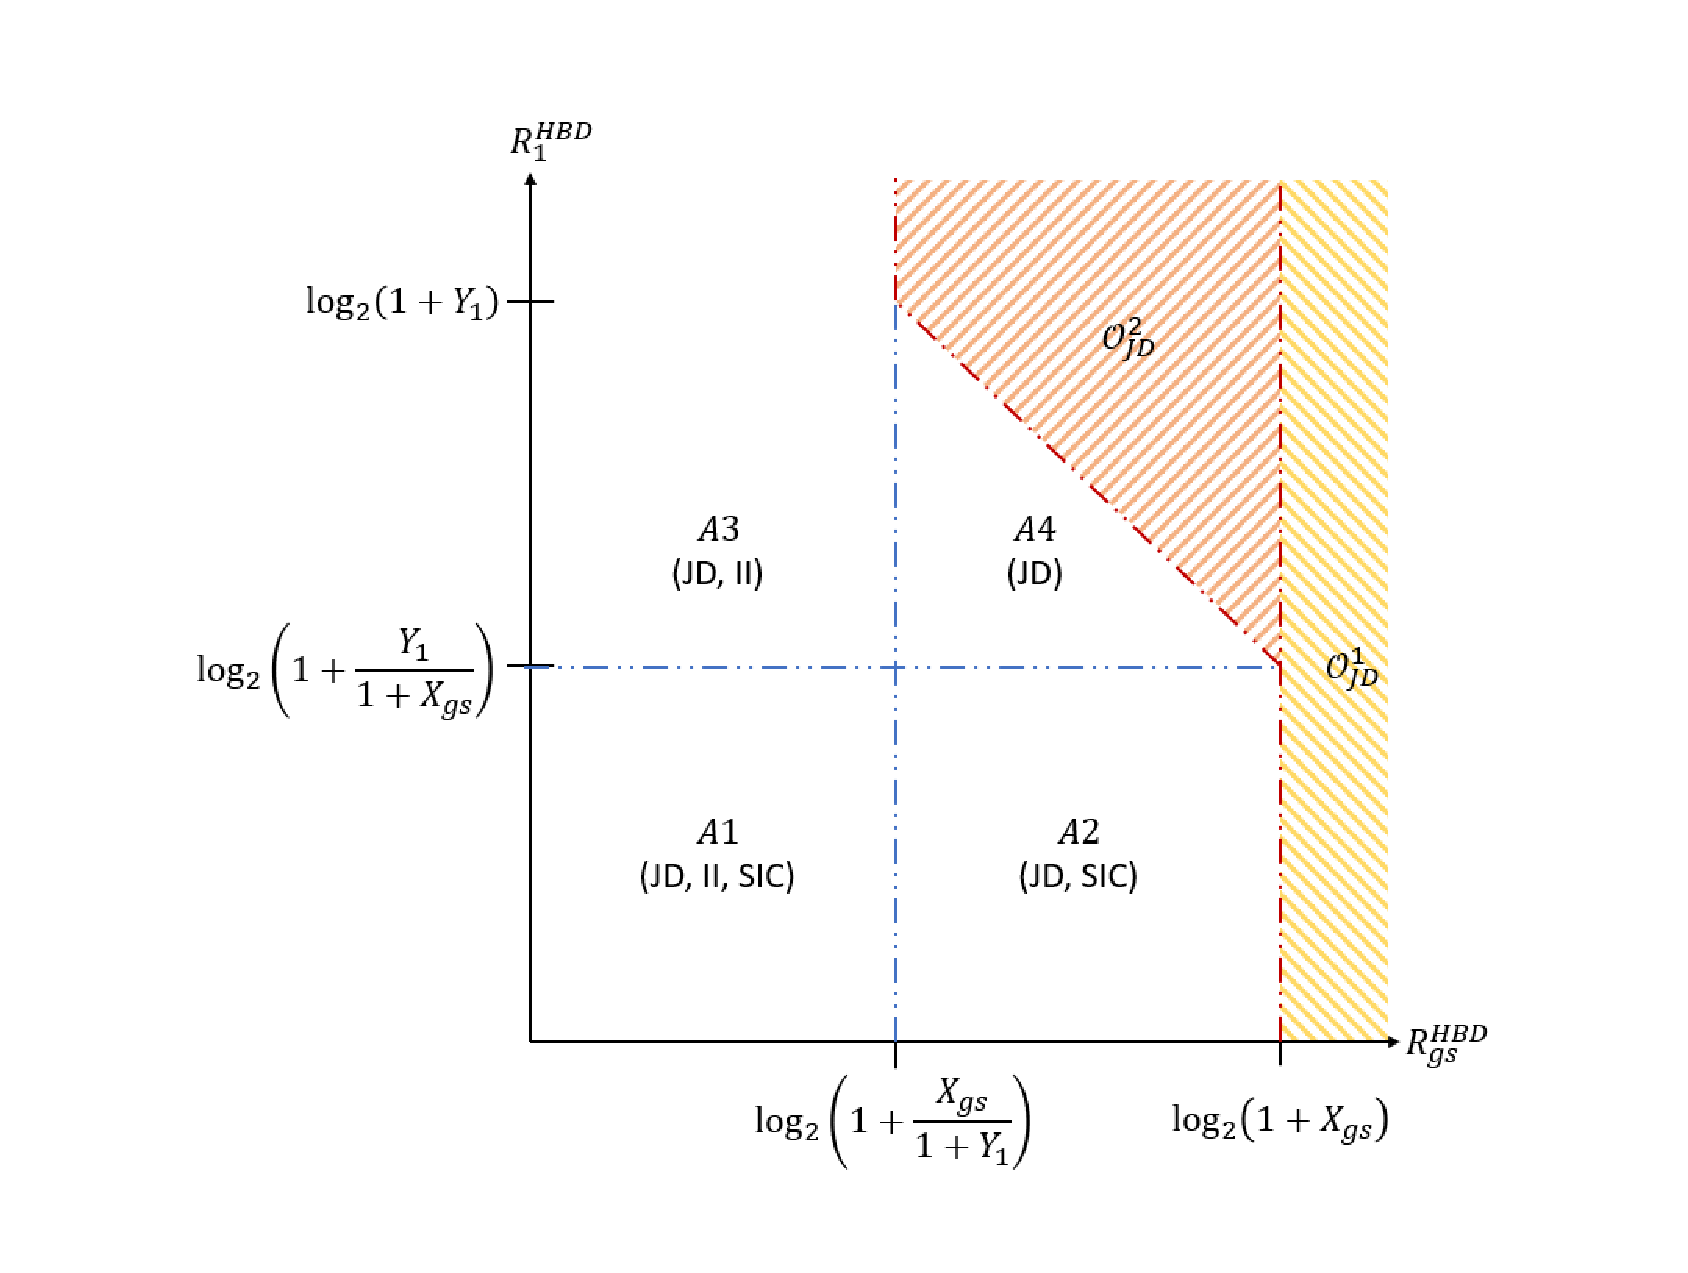
\includegraphics [width=0.6\columnwidth]{chap4_fig/rate_regions.eps} 
\vspace{-0.5cm}
\caption{The achievable instantaneous rate regions of the II, SIC and joint detectors (unshaded areas) at UAV-2 with respect to the transmission rates of the GS $\big(R_{GS}^{HBD}\big)$ and UAV-1 $\big(R_{1}^{HBD}\big)$. The shaded areas, $\mathcal{O}_{JD}^{1}$ and $\mathcal{O}_{JD}^{2}$, respectively denote the outage region of the joint detector if SOI detection fails or if the sum rate constraint is not met.}
\vspace{-0.25cm}
\label{fig:JD_HBD_UCS_rate_regions}
\end{figure}

To mitigate inter-UAV interference, the joint detector at UAV-2 simultaneously detects both SOI and interference from GS and UAV-1, respectively. The resultant instantaneous achievable rate region of the joint detector ($A1$ to $A4$), along with the II detector ($A1$ and $A3$) and the SIC detector ($A1$ and $A2$), are illustrated in Fig. \ref{fig:JD_HBD_UCS_rate_regions}. Based on the instantaneous achievable rate region, the HBD outage event of the joint detector at UAV-2 is defined as:
%%%%%%%%%%%%%%%%%%%%%%%%%%%%%%%%%%%%%%%%%%%%%%%%%%%%%%%%%%%%%%%%%%%%%%%%%%%%%%%%%
\begin{eqnarray}
							& \mathcal{O}_{2}^{HBD(JD)} & = \mathcal{O}_{JD}^{1} \cup \mathcal{O}_{JD}^{2} \label{JD_HBD_UCS_outage_JD_overall} \\
\text{where}	& \mathcal{O}_{JD}^{1} 			& = \bigg\{h_{g,2}, h_{1,2} : R_{gs}^{HBD} > \log_{2}\bigg(1+X_{gs}\bigg)\bigg\}, \label{JD_HBD_UCS_outage_JD_soi}\\
							& \mathcal{O}_{JD}^{2} 			& = \bigg\{h_{g,2}, h_{1,2} : R_{1}^{HBD} + R_{gs}^{HBD} > \log_{2}\bigg(1+X_{gs}+Y_{1} \bigg), \nonumber\\
							&														& \hspace{0.5cm} \log_{2}\bigg(1+\frac{X_{gs}}{1+Y_{1}} \bigg) \leq R_{gs}^{HBD} \hspace{-0.05cm} \leq \hspace{-0.05cm} \log_{2}\bigg(1+X_{gs}\bigg) \bigg\} \label{JD_HBD_UCS_outage_JD_int}.
\end{eqnarray}
%%%%%%%%%%%%%%%%%%%%%%%%%%%%%%%%%%%%%%%%%%%%%%%%%%%%%%%%%%%%%%%%%%%%%%%%%%%%%%%%%
\begin{remark} \label{remark_jd}
\textit{The joint detector outage event $\big(\mathcal{O}_{2}^{HBD(JD)}\big)$ occurs if SOI detection fails $\big(\mathcal{O}_{JD}^{1}\big)$ or if the sum rate constraint is not met $\big(\mathcal{O}_{JD}^{2}\big)$. Evidently, meeting the sum rate constraint $\big(\mathcal{O}_{JD}^{2}\big)$ enables the joint detector to attain a larger rate region than the II and the SIC detectors at the cost of complex hardware \cite{shubhi2017joint,blomer2009transmission}.}
\end{remark}

In a two-user multiple access channel, the joint detector simultaneously decodes the two user's data streams as the SOIs. An outage event occurs if either of the streams cannot be decoded \cite{narasimhan2007individual}. In contrast, only the signal from the FD-enabled GS is treated as the SOI while the signal from UAV-2 is treated as interference in this chapter. Therefore, the joint detector tries to decode only the SOI, while utilizing the structure of the interfering signal. Consequently, the interfering signal can be transmitted at a higher rate than the capacity of the interfering link \cite{bennatan2014soft}.

The advantages of the joint detector in this chapter is evident in Fig. \ref{fig:JD_HBD_UCS_rate_regions}. In particular, (\ref{JD_HBD_UCS_outage_JD_soi}) and (\ref{JD_HBD_UCS_outage_JD_int}) are obtained using the above principles. A similar decoding algorithm for an interference-limited receiver in a two-user interference channel is also investigated in \cite{bandemer2012simultaneous,nam2014advanced}, where similar achievable instantaneous rate regions were obtained. For the II and SIC detectors, the respective achievable instantaneous rate regions are obtained using the outage events definition in \cite{ernest2019outage}. Together, the achievable instantaneous rate regions in Fig. \ref{fig:JD_HBD_UCS_rate_regions} form the basis for Remark \ref{remark_jd}.

Next, let $\overline{\alpha}\big(q,\Omega,K,\gamma\big)$ be the CDF expansion of a Rician fading channel, which is defined as:
%%%%%%%%%%%%%%%%%%%%%%%%%%%%%%%%%%%%%%%%%%%%%%%%%%%%%%%%%%%%%%%%%%%%%%%%%%%%%%%%%
\begin{eqnarray} \label{JD_HBD_UCS_alpha_func}
\overline{\alpha}\big(q,\Omega,K,\gamma\big) = (-1)^q \exp(-K) \frac{{L_q}^{(0)}(K)}{(1+q)!} \Bigg(\frac{(1+K)}{\Omega}\gamma\Bigg)^{q+1},
\end{eqnarray}
%%%%%%%%%%%%%%%%%%%%%%%%%%%%%%%%%%%%%%%%%%%%%%%%%%%%%%%%%%%%%%%%%%%%%%%%%%%%%%%%%
where $q$, $\Omega$, $K$ and $\gamma$ represents an arbitrary non-negative integer, average received power of a Rician signal, Rician $K$ factor and threshold, respectively, and ${L_q}^{(0)}(\bullet)$ represents the $q$-th degree, zero-order Laguerre polynomials \cite{andras2011generalized}. Then, the closed-form outage probability expression for the joint detector is presented in the following theorem.

\begin{theorem}
The closed-form expression for the outage probability with joint detector at UAV-2 is:
%%%%%%%%%%%%%%%%%%%%%%%%%%%%%%%%%%%%%%%%%%%%%%%%%%%%%%%%%%%%%%%%%%%%%%%%%%%%%%%%%
\begin{eqnarray} \label{JD_HBD_UCS_P_out_as2_JD}
Pr\big(\mathcal{O}_{2}^{HBD(JD)}\big) & \approx & 1 - Q_1\left( \sqrt{2K_{X_{gs}}}, \sqrt{\frac{2(K_{X_{gs}}+1)\gamma_{th,2}^{HBD}}{\Omega_{X}\alpha_{g,2}}} \right) \nonumber\\
& & \hspace{0cm} + \sum_{n=0}^{K_{tr}} \hspace{-0.05cm} \sum_{i=0}^{n} \hspace{-0.05cm} \sum_{j=0}^{i+1} \overline{\alpha}(i,\Omega_X\alpha_{1,2},K_{Y_1},1) \overline{\alpha}(n-i,\Omega_X\alpha_{g,2},K_{X_{gs}},1) \binom{i+1}{j} \nonumber\\
& & \hspace{1cm} \times (-1)^{i+1} G_1\big(i,j,b_2,\gamma_{th,2}^{HBD}\big) \frac{G_2\big(j+n-i+1,b_1,\gamma_{th,2}^{HBD}\big)}{j+n-i+1},
\end{eqnarray}
%%%%%%%%%%%%%%%%%%%%%%%%%%%%%%%%%%%%%%%%%%%%%%%%%%%%%%%%%%%%%%%%%%%%%%%%%%%%%%%%%
where $K_{tr}$ is the truncation order, $\gamma_{th,2}^{HBD} = 2^{R_{gs}^{HBD}}-1$ is the threshold, $b_1 = 2^{R_{1}^{HBD}}(2^{R_{gs}^{HBD}}-1)$, $b_2 = 2^{R_{1}^{HBD}+R_{gs}^{HBD}}-1$, $G_1\big(i,j,b_2,\gamma_{th,2}^{HBD}\big)=(-b_2)^{i+1-j} - (-\gamma_{th,2}^{HBD})^{-j}$, $G_2\big(j+n-i+1,b_1,\gamma_{th,2}^{HBD}\big) = (b_1)^{j+n-i+1} - (\gamma_{th,2}^{HBD})^{j+n-i+1}$ and $Q_1\left(\cdot,\cdot\right)$ is the Marcum Q function \cite{andras2011generalized}
\end{theorem}
\begin{proof}
The proof can be found in Appendix \ref{JD_HBD_UCS_JD_proof}.
\end{proof}

\begin{remark}
\textit{The first two terms on the RHS of (\ref{JD_HBD_UCS_P_out_as2_JD}) are due to the outage event $\mathcal{O}_{JD}^{1}$. These two terms also correspond to the outage probability of an interference-free UAV-2. The third term on the RHS of (\ref{JD_HBD_UCS_P_out_as2_JD}) is due to the outage event $\mathcal{O}_{JD}^{2}$, where the functions $\overline{\alpha}(i,\Omega_X\alpha_{1,2},K_{Y_1},1)$ and $\overline{\alpha}(n-i,\Omega_X\alpha_{g,2},K_{X_{gs}},1)$ are due to the inter-UAV interference and SOI, respectively. From (\ref{JD_HBD_UCS_P_out_as2_JD}), it is evident that failure to either detect the SOI or meet the sum rate constraint contributes to outage probability.}
\end{remark}

The expression in (\ref{JD_HBD_UCS_P_out_as2_JD}) is only valid if the power series in the second term on the RHS converges, which is proven in the following theorem.
\begin{theorem}
The power series in (\ref{JD_HBD_UCS_P_out_as2_JD}) has a convergence radius of $\infty$.
\end{theorem}
\begin{proof}
The proof can be found in Appendix \ref{JD_HBD_UCS_JD_convg_proof}.
\end{proof}

It should be noted that the differentiation of a convergent power series, e.g., (\ref{JD_HBD_UCS_appdx_JD_9}), is also valid within the convergence radius \cite{amann2005analysis,gradshteyn2014table}, which is useful for deriving expressions related to finite SNR analysis in the next section.

It is known that the joint detector is effective when strong interference is encountered \cite{zahavi2017cooperation,zhou2015mac,shubhi2017joint,blomer2009transmission}. To investigate the effect of strong inter-UAV interference, we evaluate the limit of $\overline{\alpha}(i,\Omega_X\alpha_{1,2},K_{Y_1},1)$ with respect to $\alpha_{1,2}$. In particular, we evaluate the limit for the extreme case of very strong inter-UAV interference ($\alpha_{1,2} \to \infty$), using the same approach in \cite[eq.(11)]{ernest2019outage}. From (\ref{JD_HBD_UCS_alpha_func}) and (\ref{JD_HBD_UCS_P_out_as2_JD}), it can be seen that the outage probability with joint detector approaches that of an interference-free UAV-2 as $\alpha_{1,2} \to \infty$. Hence, the joint detector is suitable for strong interference scenarios since the detection of the SOI becomes easier. Although the SIC is also known to perform well at very strong inter-UAV interference levels, the joint detector still outperforms the SIC detector at high SNRs, as will be shown in Section \ref{JD_HBD_UCS_num_results_sec}. More importantly, (\ref{JD_HBD_UCS_P_out_as2_JD}) also suggests the possibility of the joint detector attaining near-genie-aided (\textcolor{black}{near perfect}), i.e., interference-free, outage performance when interference is sufficiently strong.

\subsection{Benchmark Schemes and System Level Outage Probability} \label{JD_HBD_UCS_sub_sec_ref_schemes_outage}

\begin{table}[]
\centering
\caption{References for the outage probability of the benchmark schemes}
\label{table:JD_HBD_UCS_ref_schemes_outage}
\scalebox{0.7}{\begin{tabular}{ccc}
\hline 
Protocol/Detector						& Notation 																	& Reference \\ \hline \hline \vspace{0.05cm}
II Detector at GS			&	$Pr\big(\mathcal{O}_{gs}^{HBD}\big)$			& \cite[eq. (6)]{ernest2019outage}  \\ \vspace{0.05cm}
II Detector at UAV-2 	& $Pr\big(\mathcal{O}_{2}^{HBD(II)}\big)$ 	& \cite[eq. (8)]{ernest2019outage} \\ \vspace{0.05cm} 
SIC Detector at UAV-2	&	$Pr\big(\mathcal{O}_{2}^{HBD(SIC)}\big)$	& \cite[eq. (10)]{ernest2019outage}  \\ \vspace{0.05cm}
HD-UCS at GS					&	$Pr\big(\mathcal{O}_{gs}^{HD}\big)$				& \cite[eq. (12)]{ernest2019outage}  \\ \vspace{0.05cm}
HD-UCS at UAV-2				&	$Pr\big(\mathcal{O}_{2}^{HD}\big)$				& \cite[eq. (13)]{ernest2019outage}  \\ \hline
\end{tabular}} \vspace{-0.5cm}
\end{table}


In this chapter, the II detector, SIC detector, and the HD-UCS are also considered at UAV-2. These schemes are treated as benchmark schemes as the associated outage probability expressions are already available in the literature, with the references provided in Table \ref{table:JD_HBD_UCS_ref_schemes_outage}. At the GS, residual SI is present and thus, the GS effectively adopts an II detector. The outage probability expression for the GS is also available in the literature and is similarly provided in Table \ref{table:JD_HBD_UCS_ref_schemes_outage}.

To compare the overall performance of the HBD-UCS against the HD-UCS at the system level, we define the HBD and HD system level outage probability as:
\begin{eqnarray}
P_{out,system}^{\beta} & = & \max\big\{Pr\big(\mathcal{O}_{gs}^{HBD}\big),Pr\big(\mathcal{O}_{2}^{\beta}\big)\big\}, \\
P_{out,system}^{HD} & = & \max\big\{Pr\big(\mathcal{O}_{gs}^{HD}\big),Pr\big(\mathcal{O}_{2}^{HD}\big)\big\}
\end{eqnarray}
where $\beta \in \{HBD(II), HBD(SIC), HBD(JD)\}$. The defined HBD system level outage probability enables the identification of performance bottleneck in the proposed HBD-UCS.

% Section: Finite SNR Diversity Gain
\section{Finite SNR Analysis}

In this section, the necessary mathematical analysis and closed-form expressions for finite SNR diversity gains are presented for both fixed and variable transmission rate systems, with detailed derivations omitted for brevity.
%%%%%%%%%%%%%%%%%%%%%%%%%%%%%%%%%%%%%%%%%%%%%%%%%%%%%%%%%%%%%%%%%%%%%%%%%%%%%%%%%%%%%%%%%%%%%%%%%%%%%%%%%%%%%%%%%%%%%%%%%%%%%%%%%%%%%%%%%
\subsection{Finite SNR Diversity Gain}

The asymptotic diversity gain of a system, given by Zheng and Tse \cite[eq. (3)]{zheng2003diversity}, quantifies the outage probability decay rate at high SNR. However, the definition in \cite[eq. (3)]{zheng2003diversity} may not be accurate at low to moderate SNR ranges \cite{shin2008diversity}. 

To this end, finite SNR diversity gain definitions for low to moderate SNR ranges have been presented by Narasimhan \cite[eq. (5)]{narasimhan2006finite} and Shin et al. \cite{shin2008diversity}. Let $\mathcal{O}$, $Pr\big(\mathcal{O}\big)$, $R$, $\gamma$ and $\Omega$ be the outage event, outage probability, transmission rate, threshold and average received power with unit noise variance, respectively. Then, the finite SNR diversity gain ($d_f$) of a given system is \cite[eq. (5)]{narasimhan2006finite}:
%%%%%%%%%%%%%%%%%%%%%%%%%%%%%%%%%%%%%%%%%%%%%%%%%%%%%%%%%%%%%%%%%%%%%%%%%%%%%%%%%
\begin{eqnarray} \label{JD_HBD_UCS_df}
d_f = \frac{-\Omega}{Pr\big(\mathcal{O}\big)}\frac{\partial}{\partial\Omega}Pr\big(\mathcal{O}\big).
\end{eqnarray}
%%%%%%%%%%%%%%%%%%%%%%%%%%%%%%%%%%%%%%%%%%%%%%%%%%%%%%%%%%%%%%%%%%%%%%%%%%%%%%%%%

At high SNR, (\ref{JD_HBD_UCS_df}) is consistent with the asymptotic diversity gain definition given by Zheng and Tse \cite{zheng2003diversity}, as proven by Shin et al. \cite{shin2008diversity} and Heidarpour et al. \cite{heidarpour2017finite}. Moreover, (\ref{JD_HBD_UCS_df}) enables system designers to investigate the impact of residual SI and inter-UAV interference in HBD-UCS and to quantify potential outage performance improvements through code designs for the II, SIC and joint detectors at typical operating SNR ranges. 

\subsection{Finite SNR DMT Parameters}
For variable transmission rate systems, i.e., adaptive rate systems, the finite SNR multiplexing gain $r_f$ is defined as \cite[eq. (4)]{narasimhan2006finite}:
%%%%%%%%%%%%%%%%%%%%%%%%%%%%%%%%%%%%%%%%%%%%%%%%%%%%%%%%%%%%%%%%%%%%%%%%%%%%%%%%%
\begin{eqnarray} \label{JD_HBD_UCS_rf}
r_f = \frac{R(\Omega)}{\log_2(1+\Omega)}.
\end{eqnarray}
%%%%%%%%%%%%%%%%%%%%%%%%%%%%%%%%%%%%%%%%%%%%%%%%%%%%%%%%%%%%%%%%%%%%%%%%%%%%%%%%%

In variable transmission rate systems, $Pr\big(\mathcal{O}\big)$ is computed with respect to $\gamma=(1+\Omega)^{r_f}-1$. The finite SNR multiplexing gain indicates the sensitivity of $\gamma$ when $\Omega$ changes, and similar to (\ref{JD_HBD_UCS_df}), (\ref{JD_HBD_UCS_rf}) has also been proven by Shin et al. \cite{shin2008diversity} and Heidarpour et al. \cite{heidarpour2017finite} to be consistent with asymptotic multiplexing gain in \cite[eq. (3)]{zheng2003diversity}.

Let $\Delta(\Omega)=\widehat{\Omega}-\Omega$ where $\widehat{\Omega}>\Omega$. Then, extending upon (\ref{JD_HBD_UCS_df}), the finite SNR diversity gain for variable transmission rate systems (denoted as $d_{f}^{*}$) is \cite[eq. (36)]{shin2008diversity}:
%%%%%%%%%%%%%%%%%%%%%%%%%%%%%%%%%%%%%%%%%%%%%%%%%%%%%%%%%%%%%%%%%%%%%%%%%%%%%%%%%
\begin{eqnarray}
d_f^* & = & \frac{-\Omega}{Pr\big(\mathcal{O}\big)} \lim_{\Delta(\Omega)\to0} \Big[\frac{Pr\big(\mathcal{\widehat{O}}\big) - Pr\big(\mathcal{O}\big)}{\Delta(\Omega)}\Big] \label{JD_HBD_UCS_df_var_rate1} \\
& = & \frac{-\Omega}{Pr\big(\mathcal{O}\big)} \frac{\partial}{\partial\Delta(\Omega)} Pr\big(\mathcal{\widehat{O}}\big) \bigg|_{\Delta(\Omega)=0,} \label{JD_HBD_UCS_df_var_rate2}
\end{eqnarray}
%%%%%%%%%%%%%%%%%%%%%%%%%%%%%%%%%%%%%%%%%%%%%%%%%%%%%%%%%%%%%%%%%%%%%%%%%%%%%%%%%
where (\ref{JD_HBD_UCS_df_var_rate2}) is obtained from (\ref{JD_HBD_UCS_df_var_rate1}) by applying L'hopital's rule with respect to $\Delta(\Omega)$, $\mathcal{\widehat{O}}$ is the outage event with respect to $R\big(\Omega+\Delta(\Omega)\big)$ and $Pr\big(\mathcal{\widehat{O}}\big)$ is the outage probability with average received power $\widehat{\Omega}=\Omega+\Delta(\Omega)$, threshold $\widehat{\gamma}=[1+\Omega+\Delta(\Omega)]^{r_f}-1$ and $Pr\big(\mathcal{\widehat{O}}\big)=Pr\big(\mathcal{O}\big)$ when $\Delta(\Omega)=0$. Furthermore, although not explicitly shown in (\ref{JD_HBD_UCS_df_var_rate2}), we define $d_f^*$ to be non-negative, i.e., $d_f^* = \max\bigg\{0, \frac{-\Omega}{Pr\big(\mathcal{O}\big)} \frac{\partial}{\partial\Delta(\Omega)} Pr\big(\mathcal{\widehat{O}}\big) \bigg|_{\Delta(\Omega)=0} \bigg\}$, as it is a measure of the negative slope of the outage probability curve \cite{narasimhan2006finite}.

Let the normalized $n^{th}$ moment of a RV $Z$ be:
%%%%%%%%%%%%%%%%%%%%%%%%%%%%%%%%%%%%%%%%%%%%%%%%%%%%%%%%%%%%%%%%%%%%%%%%%%%%%%%%%
\begin{eqnarray} \label{JD_HBD_UCS_norm_moment}
M\{Z^{n}\}=\frac{E\{Z^{n}\}}{(\Omega)^{n}}
\end{eqnarray}
%%%%%%%%%%%%%%%%%%%%%%%%%%%%%%%%%%%%%%%%%%%%%%%%%%%%%%%%%%%%%%%%%%%%%%%%%%%%%%%%%
and let function $g(i,j,\Omega,r_f)$ be:
%%%%%%%%%%%%%%%%%%%%%%%%%%%%%%%%%%%%%%%%%%%%%%%%%%%%%%%%%%%%%%%%%%%%%%%%%%%%%%%%%
\begin{eqnarray} \label{JD_HBD_UCS_g_func}
g(i,j,\Omega,r_f) & = & \big([1 + \Omega]^{r_f}-1\big)^{i} (\Omega)^{j} \Big[ \big([1 + \Omega]^{r_f} - 1\big) \frac{j}{\Omega} + (i+1)(r_f)(1 + \Omega)^{r_f-1} \Big], \nonumber \\
\end{eqnarray}
%%%%%%%%%%%%%%%%%%%%%%%%%%%%%%%%%%%%%%%%%%%%%%%%%%%%%%%%%%%%%%%%%%%%%%%%%%%%%%%%%
where $i$ and $j$ are integers. The function $g(i,j,\Omega,r_f)$ reflects the outage probability decay rate of a variable transmission rate scheme due to average received power ($\Omega$) and finite SNR multiplexing gain ($r_f$) \cite{ernest2019outage}.

It should be noted that the resultant finite SNR diversity gain expression in (\ref{JD_HBD_UCS_df_var_rate2}) is based on \cite[eq. (36)]{shin2008diversity} and \cite[eq. (5)]{narasimhan2006finite}. Although \cite[eq. (36)]{shin2008diversity} and \cite[eq. (5)]{narasimhan2006finite} evaluated finite SNR diversity gain through different approaches and definitions, the former is based on the latter. Hence, (\ref{JD_HBD_UCS_df_var_rate2}) shows that both works are unified under the same principles. Similar to (\ref{JD_HBD_UCS_df}), the impact of residual SI and inter-UAV interference in adaptive HBD-UCS can be analyzed through (\ref{JD_HBD_UCS_df_var_rate2}).

%%%%%%%%%%%%%%%%%%%%%%%%%%%%%%%%%%%%%%%%%%%%%%%%%%%%%%%%%%%%%%%%%%%%%%%%%%%%%%%%%%%%%%%%%%%%%%%%%%%%%%%%%%%%%%%%%%%%%%%%%%%%%%%%%%%%%%%%
\subsection{Finite SNR Diversity Gain and DMT for HBD Systems}

For the joint detector, the finite SNR diversity gain ($d_{f,2}^{HBD(JD)}$) is given in the following proposition.
\begin{proposition} 
The finite SNR diversity gain at UAV-2 for the joint detector is:
%%%%%%%%%%%%%%%%%%%%%%%%%%%%%%%%%%%%%%%%%%%%%%%%%%%%%%%%%%%%%%%%%%%%%%%%%%%%%%%%%
\begin{eqnarray} \label{JD_HBD_UCS_df_fixed_UAV2_JD}
d_{f,2}^{HBD(JD)} & \approx & \frac{-\Omega_X}{Pr\big(\mathcal{O}_{2}^{HBD(JD)}\big)} \Bigg[ \sum_{m=0}^{K_{tr}} \overline{\alpha}\big(m,\alpha_{g,2},K_{X_{gs}},\gamma_{th,2}^{HBD}\big) \nonumber\\
& & \hspace{-0cm} \times (-m-1) (\Omega_{X})^{-m-2} + \sum_{n=0}^{K_{tr}}\sum_{i=0}^{n}\sum_{j=0}^{i+1} \overline{\alpha}(i,\alpha_{1,2},K_{Y_1},1) \nonumber\\
& & \hspace{-0cm} \times \overline{\alpha}(n-i,\alpha_{g,2},K_{X_{gs}},1) \binom{i+1}{j}(-1)^{i+1} G_1\big(i,j,b_2,\gamma_{th,2}^{HBD}\big) \nonumber\\
& & \hspace{-0cm} \times \frac{G_2\big(j+n-i+1,b_1,\gamma_{th,2}^{HBD}\big)}{j+n-i+1} (-n-2)(\Omega_X)^{-n-3} \Bigg].
\end{eqnarray}
%%%%%%%%%%%%%%%%%%%%%%%%%%%%%%%%%%%%%%%%%%%%%%%%%%%%%%%%%%%%%%%%%%%%%%%%%%%%%%%%%
\end{proposition}
\begin{proof}
At UAV-2, $d_{f,2}^{HBD(JD)}$ can be obtained from (\ref{JD_HBD_UCS_P_out_as2_JD}) and (\ref{JD_HBD_UCS_df}).
\end{proof}

The expression in (\ref{JD_HBD_UCS_df_fixed_UAV2_JD}) is accurate even at low to moderate $\Omega_X$, and it is useful in evaluating the impact of inter-UAV interference on outage probability decay trends. \textcolor{black}{\footnote{\textcolor{black}{To analytically gauge the accuracy of the new power series expressions presented in this Chapter, one will need to conduct a truncation analysis. Work in this direction is left as an open research challenge which can be addressed in future studies.}}} To uncover the asymptotic outage behavior for the joint detector, we evaluate (\ref{JD_HBD_UCS_df_fixed_UAV2_JD}) at high $\Omega_X$, as shown in the following corollary.

\begin{corollary} \label{JD_HBD_UCS_asymptotic_JD}
At UAV-2, the joint detector achieves full diversity at high SNR regimes.
\begin{proof}
To prove Corollary \ref{JD_HBD_UCS_asymptotic_JD}, we have to show that 
\begin{eqnarray} \label{JD_HBD_UCS_asymp_df_fixed_UAV2_JD}
\lim_{\Omega_X\to\infty} \frac{-\Omega_X}{Pr\big(\mathcal{O}_{2}^{HBD(JD)}\big)} \frac{\partial}{\partial\Omega_X}Pr\big(\mathcal{O}_{2}^{HBD(JD)}\big) & = & 1.
\end{eqnarray}

By simplifying (\ref{JD_HBD_UCS_df_fixed_UAV2_JD}) and evaluating the limits with respect to $\Omega_X$ leads to the following expression:
%%%%%%%%%%%%%%%%%%%%%%%%%%%%%%%%%%%%%%%%%%%%%%%%%%%%%%%%%%%%%%%%%%%%%%%%%%%%%%%%%
\begin{eqnarray} \label{JD_HBD_UCS_df_fixed_UAV2_JD_2}
\lim_{\Omega_X\to\infty} d_{f,2}^{HBD(JD)} & \approx & \lim_{\Omega_X\to\infty} \frac{-1}{\Omega_X \cdot Pr\big(\mathcal{O}_{2}^{HBD(JD)}\big)} \Bigg[ \sum_{m=0}^{K_{tr}} \overline{\alpha}\big(m,\alpha_{g,2},K_{X_{gs}},\gamma_{th,2}^{HBD}\big) (-m-1) (\Omega_{X})^{-m} \nonumber\\
& & \hspace{-0cm} + \sum_{n=0}^{K_{tr}}\sum_{i=0}^{n}\sum_{j=0}^{i+1} \overline{\alpha}(i,\alpha_{1,2},K_{Y_1},1) \overline{\alpha}(n-i,\alpha_{g,2},K_{X_{gs}},1) \binom{i+1}{j} \nonumber\\
& & \hspace{1cm} \times G_1\big(i,j,b_2,\gamma_{th,2}^{HBD}\big) \frac{G_2\big(j+n-i+1,b_1,\gamma_{th,2}^{HBD}\big) (-n-2)}{(-1)^{-i-1}(j+n-i+1)(\Omega_X)^{n+1}} \Bigg].
\end{eqnarray}
%%%%%%%%%%%%%%%%%%%%%%%%%%%%%%%%%%%%%%%%%%%%%%%%%%%%%%%%%%%%%%%%%%%%%%%%%%%%%%%%%

For the first term in the numerator of (\ref{JD_HBD_UCS_df_fixed_UAV2_JD_2}), $\lim_{\Omega_X\to\infty} \left(\Omega_X\right)^{-m} = 0$ when $m>0$ and $\lim_{\Omega_X\to\infty} \left(\Omega_X\right)^{-m} = 1$ when $m=0$. Likewise for the second term in the numerator, $\lim_{\Omega_X\to\infty} \left(\Omega_X\right)^{-n-1} = 0$ for $n\geq0$. Therefore, we only consider $m=0$ when evaluating the limit in the numerator. Repeating the same steps for the denominator in (\ref{JD_HBD_UCS_df_fixed_UAV2_JD_2}) leads to (\ref{JD_HBD_UCS_asymp_df_fixed_UAV2_JD})
\end{proof}
\end{corollary}

From (\ref{JD_HBD_UCS_asymp_df_fixed_UAV2_JD}), the joint detector's diversity gain is better than the II and SIC detectors, as shown in \cite[eq. (28)]{ernest2019outage}, and is equivalent to an HD-UCS \cite[eq. (31)]{ernest2019outage}.

For the GS and UAV-2 operating under a variable rate transmission scheme, let the variable transmission rate of UAV-1 and GS be $R_1^{HBD}(\Omega_X)=r_{f,1}\log_2(1+\Omega_X)$ and $R_{gs}^{HBD}(\Omega_X)=r_{f,gs}\log_2(1+\Omega_X)$, respectively. Also, let the threshold at GS and UAV-2 be $\gamma_{th,gs}^{HBD} = [1+\Omega_X]^{r_{f,1}}-1$ and $\gamma_{th,2}^{HBD} = [1+\Omega_X]^{r_{f,gs}}-1$, respectively. Then, the variable rate finite SNR diversity gain expressions are presented in the following propositions.
\begin{proposition}
At GS, the variable rate finite SNR diversity gain is:
%%%%%%%%%%%%%%%%%%%%%%%%%%%%%%%%%%%%%%%%%%%%%%%%%%%%%%%%%%%%%%%%%%%%%%%%%%%%%%%%%
\begin{eqnarray} \label{JD_HBD_UCS_df_var_gs}
d_{f,gs}^{HBD*} & \approx & \frac{-\Omega_X}{Pr\big(\mathcal{O}_{gs}^{HBD}\big)} \sum_{q=0}^{K_{tr}}\sum_{l_1+l_2+l_3=q+1} \overline{\alpha}\big(q,1,K_{X_1},1\big) \frac{(q+1)!}{l_1! \cdot l_2! \cdot l_3!} \nonumber\\
& & \hspace{1cm} \times M\{Y_{si,1}^{l_1}\} M\{Y_{si,2}^{l_2}\} g(q,l_1+l_2-q-1,\Omega_X,r_{f,1}).
\end{eqnarray}
%%%%%%%%%%%%%%%%%%%%%%%%%%%%%%%%%%%%%%%%%%%%%%%%%%%%%%%%%%%%%%%%%%%%%%%%%%%%%%%%%
\end{proposition}
\begin{proof}
Let $\Omega=\Omega_X$, $\widehat{\Omega}=\widehat{\Omega}_X$ and $\gamma = \gamma_{th,gs}^{HBD}=[1+\Omega_X]^{r_{f,1}}-1$ and $\mathcal{O} = \mathcal{O}_{gs}^{HBD}$. Then, $d_{f,gs}^{HBD*}$ can be obtained through algebraic manipulations by substituting \cite[eq. (6)]{ernest2019outage} into (\ref{JD_HBD_UCS_df_var_rate2}).
\end{proof}

\begin{proposition}
At UAV-2, the variable rate finite SNR diversity gain with the II and the SIC detectors are given in (\ref{JD_HBD_UCS_df_var_UAV2_II}) and (\ref{JD_HBD_UCS_df_var_UAV2_SIC}), respectively.
%%%%%%%%%%%%%%%%%%%%%%%%%%%%%%%%%%%%%%%%%%%%%%%%%%%%%%%%%%%%%%%%%%%%%%%%%%%%%%%%%
%\begin{eqnarray} 
%d_{f,2}^{HBD(II)*} & \approx & \frac{-\Omega_X}{Pr\big(\mathcal{O}_{2}^{HBD(II)}\big)} \sum_{q=0}^{K_{tr}} \sum_{l=0}^{q+1} \overline{\alpha}\big(q,\alpha_{g,2}, K_{X_{gs}}, 1\big) \nonumber\\
%& & \hspace{-0.5cm} \times \binom{q+1}{l} M\{Y_1^l\} g(q,l-q-1,\Omega_X,r_{f,gs}) \label{df_var_UAV2_II} \\
%d_{f,2}^{HBD(SIC)*} & \approx & \frac{-\Omega_X}{Pr\big(\mathcal{O}_{2}^{HBD(SIC)}\big)} \Bigg[ \sum_{q=0}^{K_{tr}}\sum_{l=0}^{q+1} \overline{\alpha}\big(q,\alpha_{1,2},K_{Y_{1}},1\big) \nonumber\\
%& & \hspace{-2cm} \times \binom{q+1}{l} M\{X_{gs}^l\} g(q,l-q-1,\Omega_X,r_{f,1}) \nonumber\\
%& & \hspace{-2cm} + \sum_{m=0}^{K_{tr}} \overline{\alpha}\big(m,\alpha_{g,2},K_{X_{gs}},1\big) g(m,-m-1,\Omega_X,r_{f,gs}) \nonumber\\
%& & \hspace{-2cm} - \sum_{n=0}^{K_{tr}}\sum_{i=0}^{n}\sum_{j=0}^{i+1} \overline{\alpha}\big(i,\alpha_{1,2},K_{Y_{1}},1\big) \overline{\alpha}\big(n-i,\alpha_{g,2},K_{X_{gs}},1\big) \nonumber\\
%& & \hspace{-2cm} \times \frac{\binom{i+1}{j}}{j+n-i+1} g(j+n+1,-n-2,\Omega_X,r_{f,1}) \Bigg]. \label{df_var_UAV2_SIC}
%\end{eqnarray}
%%%%%%%%%%%%%%%%%%%%%%%%%%%%%%%%%%%%%%%%%%%%%%%%%%%%%%%%%%%%%%%%%%%%%%%%%%%%%%%%%

\begin{figure*}[!t]
% ensure that we have normalsize text
\normalsize
% Store the current equation number.
\setcounter{mytempeqncnt}{\value{equation}}
% Set the equation number to one less than the one
% desired for the first equation here.
% The value here will have to changed if equations
% are added or removed prior to the place these
% equations are referenced in the main text.
\setcounter{equation}{21}
\begin{eqnarray}
d_{f,2}^{HBD(II)*} & \approx & \frac{-\Omega_X}{Pr\big(\mathcal{O}_{2}^{HBD(II)}\big)} \sum_{q=0}^{K_{tr}} \sum_{l=0}^{q+1} \overline{\alpha}\big(q,\alpha_{g,2}, K_{X_{gs}}, 1\big) \nonumber \\
 & & \hspace{5cm} \times \binom{q+1}{l} M\{Y_1^l\} g(q,l-q-1,\Omega_X,r_{f,gs}). \label{JD_HBD_UCS_df_var_UAV2_II} \\
d_{f,2}^{HBD(SIC)*} & \approx & \frac{-\Omega_X}{Pr\big(\mathcal{O}_{2}^{HBD(SIC)}\big)} \Bigg[ \sum_{q=0}^{K_{tr}}\sum_{l=0}^{q+1} \overline{\alpha}\big(q,\alpha_{1,2},K_{Y_{1}},1\big) \binom{q+1}{l} M\{X_{gs}^l\} g(q,l-q-1,\Omega_X,r_{f,1}) \nonumber \\
 & & + \sum_{m=0}^{K_{tr}} \overline{\alpha}\big(m,\alpha_{g,2},K_{X_{gs}},1\big) g(m,-m-1,\Omega_X,r_{f,gs}) - \sum_{n=0}^{K_{tr}}\sum_{i=0}^{n}\sum_{j=0}^{i+1} \overline{\alpha}\big(i,\alpha_{1,2},K_{Y_{1}},1\big) \nonumber\\
 & & \hspace{1cm} \times \overline{\alpha}\big(n-i,\alpha_{g,2},K_{X_{gs}},1\big) \frac{\binom{i+1}{j}}{j+n-i+1} g(j+n+1,-n-2,\Omega_X,r_{f,1}) \Bigg]. \label{JD_HBD_UCS_df_var_UAV2_SIC}
\end{eqnarray}
% Restore the current equation number.
\setcounter{equation}{\value{mytempeqncnt}}
\addtocounter{equation}{2}
% IEEE uses as a separator
\hrulefill
% The spacer can be tweaked to stop underfull vboxes.
\vspace*{4pt}
\end{figure*}
\begin{figure*}[!t]
% ensure that we have normalsize text
\normalsize
% Store the current equation number.
\setcounter{mytempeqncnt}{\value{equation}}
% Set the equation number to one less than the one
% desired for the first equation here.
% The value here will have to changed if equations
% are added or removed prior to the place these
% equations are referenced in the main text.
\setcounter{equation}{23}
\begin{eqnarray}
d_{f,2}^{HBD(JD)*} & \approx & \frac{-\Omega_X}{Pr\big(\mathcal{O}_{2}^{HBD(JD)}\big)} \Bigg[ \sum_{m=0}^{K_{tr}} \overline{\alpha}\big(m,\alpha_{g,2},K_{X_{gs}},1\big) g(m,-m-1,\Omega_X,r_{f,gs}) \nonumber \\
 & & + \sum_{n=0}^{K_{tr}}\sum_{i=0}^{n}\sum_{j=0}^{i+1} \overline{\alpha}(i,\alpha_{1,2},K_{Y_1},1) \overline{\alpha}(n-i,\alpha_{g,2},K_{X_{gs}},1) \binom{i+1}{j} \frac{(-1)^{i+1}}{j+n-i+1} \nonumber \\
 & & \hspace{0.5cm} \times \bigg( G_1\big(i,j,b_2,\gamma_{th,2}^{HBD}\big) G_2\big(j+n-i+1,b_1,\gamma_{th,2}^{HBD}\big) \frac{-n-2}{(\Omega_X)^{n+3}} \nonumber\\
 & & \hspace{1cm} + (\Omega_X)^{-n-2} \Big[ G_1\big(i,j,b_2,\gamma_{th,2}^{HBD}\big) G_2^{'}\big(j+n-i+1,b_1,\gamma_{th,2}^{HBD}\big) \nonumber \\
 & & \hspace{2cm} + G_2\big(j+n-i+1,b_1,\gamma_{th,2}^{HBD}\big) G_1^{'}\big(i,j,b_2,\gamma_{th,2}^{HBD}\big) \Big] \bigg) \Bigg]. \label{JD_HBD_UCS_df_var_UAV2_JD}
\end{eqnarray}
% Restore the current equation number.
\setcounter{equation}{\value{mytempeqncnt}}
\addtocounter{equation}{1}
% IEEE uses as a separator
\hrulefill
% The spacer can be tweaked to stop underfull vboxes.
\vspace*{4pt}
\end{figure*}

\end{proposition}
\begin{proof}
Let $\Omega=\Omega_X$, $\widehat{\Omega}=\widehat{\Omega}_X$ and $\gamma=\gamma_{th,2}^{HBD}=[1+\Omega_X]^{r_{f,gs}}-1$ and $\mathcal{O} = \mathcal{O}_{2}^{HBD,i}, i \in \{II,SIC\}$. Then, $d_{f,2}^{HBD(II)*}$ and $d_{f,2}^{HBD(SIC)*}$ can be obtained through algebraic manipulations by respectively substituting \cite[eq. (8)]{ernest2019outage} and \cite[eq. (10)]{ernest2019outage} into (\ref{JD_HBD_UCS_df_var_rate2}). 
\end{proof}

\begin{proposition}
At UAV-2, the variable rate finite SNR diversity gain for the joint detector is given in (\ref{JD_HBD_UCS_df_var_UAV2_JD}), where:
%%%%%%%%%%%%%%%%%%%%%%%%%%%%%%%%%%%%%%%%%%%%%%%%%%%%%%%%%%%%%%%%%%%%%%%%%%%%%%%%%
\begin{eqnarray}
G_1^{'}\big(i,j,b_2,\gamma_{th,2}^{HBD}\big) & = & (i+1-j)(-b_2)^{i-j}(-(r_{f,1} + r_{f,gs})) \nonumber\\
& & \hspace{0.5cm} \times (1+\Omega_X)^{(r_{f,1} + r_{f,gs})-1} - \frac{j(r_{f,gs}) (1+\Omega_X)^{r_{f,gs}-1}}{\big(-\gamma_{th,2}^{HBD}\big)^{j+1}} \nonumber
\end{eqnarray}
\vspace{-0.75cm}
\begin{eqnarray}
G_2^{'}\big(j+n-i+1,b_1,\gamma_{th,2}^{HBD}\big) & = & (j+n-i+1)(b_1)^{j+n-i} \nonumber\\
& & \hspace{0.5cm} \times \big[(r_{f,1} + r_{f,gs})(1+\Omega_X)^{r_{f,1} + r_{f,gs}-1} - r_{f,1}(1+\Omega_X)^{r_{f,1}-1}\big] \nonumber\\
& & \hspace{1cm} - (j+n-i+1)\big(\gamma_{th,2}^{HBD}\big)^{j+n-i}(r_{f,gs}(1+\Omega_X)^{r_{f,gs}-1}) \nonumber
\end{eqnarray}
%%%%%%%%%%%%%%%%%%%%%%%%%%%%%%%%%%%%%%%%%%%%%%%%%%%%%%%%%%%%%%%%%%%%%%%%%%%%%%%%%

It should be pointed out that $G_1^{'}\big(i,j,b_2,\gamma_{th,2}^{HBD}\big)$ and $G_2^{'}\big(j+n-i+1,b_1,\gamma_{th,2}^{HBD}\big)$ are the derivative of $G_1\big(i,j,b_2,\gamma_{th,2}^{HBD}\big)$ and $G_2\big(j+n-i+1,b_1,\gamma_{th,2}^{HBD}\big)$, respectively.
\end{proposition}
\begin{proof}
Let $b_1 = (1+\Omega_X)^{r_{f,1}+r_{f,gs}} - (1+\Omega_X)^{r_{f,1}}$, $b_2 = (1+\Omega_X)^{r_{f,1}+r_{f,gs}} - 1$, $\Omega=\Omega_X$, $\widehat{\Omega}=\widehat{\Omega}_X$ and $\gamma=\gamma_{th,2}^{HBD}=[1+\Omega_X]^{r_{f,gs}}-1$ and $\mathcal{O} = \mathcal{O}_{2}^{HBD(JD)}$. Then, following a similar approach in \cite[eq. (35)]{ernest2019outage}, $d_{f,2}^{HBD(JD)*}$ is obtained from (\ref{JD_HBD_UCS_df_var_rate2}). 
\end{proof}

The finite SNR diversity gain presented earlier enables system designers to quantify the degree of improvement obtainable through an increase in SNR, thus identifying suitable detectors for various inter-UAV interference scenarios.

\subsection{Benchmark Schemes and System Level Finite SNR \\ Diversity Gain}
\begin{table}[]
\centering
\caption{References for the finite SNR diversity gains of the benchmark schemes}
\label{table:JD_HBD_UCS_ref_schemes_diversity_gain}
\scalebox{0.7}{\begin{tabular}{ccc}
\hline 
Protocol/Detector						& Notation							& Reference \\ \hline \hline \vspace{0.05cm}
II Detector at GS			&	$d_{f,gs}^{HBD}$			& \cite[eq. (24)]{ernest2019outage}  \\ \vspace{0.05cm}
II Detector at UAV-2 	& $d_{f,2}^{HBD(II)}$		& \cite[eq. (26)]{ernest2019outage} \\ \vspace{0.05cm} 
SIC Detector at UAV-2	&	$d_{f,2}^{HBD(SIC)}$	& \cite[eq. (27)]{ernest2019outage}  \\ \vspace{0.05cm}
HD-UCS at GS					&	$d_{f,gs}^{HD}$				& \cite[eq. (29)]{ernest2019outage}  \\ \vspace{0.05cm}
HD-UCS at UAV-2				&	$d_{f,2}^{HD}$				& \cite[eq. (30)]{ernest2019outage}  \\ \hline
\end{tabular}} \vspace{-0.5cm}
\end{table}

Similar to Section \ref{JD_HBD_UCS_sub_sec_ref_schemes_outage}, the diversity gains of the benchmark schemes at the GS and at UAV-2 are available in the literature, with the references provided in Table \ref{table:JD_HBD_UCS_ref_schemes_diversity_gain}. The system level diversity gains are defined as:
\begin{eqnarray}
d_{f,system}^{\beta} & = & \min\big\{ d_{f,gs}^{HBD},d_{f,2}^{\beta} \big\}, \\
d_{f,system}^{HD} & = & \min\big\{ d_{f,gs}^{HD},d_{f,2}^{HD} \big\}, \\
d_{f,system}^{\beta*} & = & \min\big\{ d_{f,gs}^{HBD*}, d_{f,2}^{\beta*} \big\}, \\
d_{f,system}^{HD*} & = & \min\big\{ d_{f,gs}^{HD*}, d_{f,2}^{HD*} \big\},
\end{eqnarray}
where $\beta \in \{HBD(II), HBD(SIC), HBD(JD)\}$. Quantifying the system level diversity gains allows for the identification of supported QoS requirements for the discussed detectors under various inter-UAV interference scenarios, \textcolor{black}{which is discussed in Section \ref{JD_HBD_UCS_num_results_sec}}.

% Section: Numerical Results
\section{Numerical and Simulation Results} \label{JD_HBD_UCS_num_results_sec}

In this section, we present the numerical and simulation results of the outage probabilities and finite SNR diversity gains at UAV-2 and at system level. Monte Carlo simulations, conducted with $10^{9}$ samples, are also presented to verify the accuracy of the outage probability computations of the various detectors. The Rician $K$ factors, i.e., $K_{X_1}$ $K_{Y_{si,1}}$, $K_{X_{gs}}$, $K_{Y_1}$, are fixed at $15$. The noise variance at GS ($\sigma_g^2$) and UAV-2 ($\sigma_2^2$) are fixed at $-115dBm$, with HD sum rate ($R_{sum}^{HD}$) and HBD sum rate ($R_{sum}^{HBD}$) set to $1$, i.e., $R_{sum}^{HD}=R_{sum}^{HBD}=1$.

\subsection{Outage and Finite SNR Diversity Gain Analysis \\ at UAV-2}

%%%%%%%%%%%%%%%%%%%%%%%%%%%%%%%%%%%%%%%%%%%%%%%%%%%%%%%%%%%%%%%%%%%%%%%%%%%%%%%%%%
% For Fig 3a:
% The joint detector achieves genie-aided outage probability at moderate and high SNR regimes. At very low SNR regimes, the joint detector attains near-genie-aided outage probability due to weaker inter-UAV interference.

% It can also be observed that both the II and the SIC detectors are interference-limited at high SNR regimes, unlike the joint detector. 

% The SIC detector attains lower outage probability under strong inter-UAV interference, e.g., $alpha_{1,2}=5$, while the II detector attains lower outage probability under weak inter-UAV interference, e.g., $alpha_{1,2}=0.5$.
%%%%%%%%%%%%%%%%%%%%%%%%%%%%%%%%%%%%%%%%%%%%%%%%%%%%%%%%%%%%%%%%%%%%%%%%%%%%%%%%%%
% For Fig 3b:
% The diversity gain expressions of the II, SIC and joint detectors are validated. As finite SNR diversity gain quantifies the decay of outage probability curves, it can be observed that the diversity gain of the various detectors corresponds to the steepness of the associated outage probability curves in Fig. 3a.

% The finite SNR diversity gain of the joint detector indicates that outage probability can be further improved at very low SNR regimes through advanced code designs. Furthermore, the joint detector attains genie-aided diversity gains as $\Omega_X \to \infty$. 

% At low SNR regimes, the joint detector achieves much better finite SNR diversity gains than the HD-UCS. However, at moderate SNR regimes, the HD-UCS achieves better diversity gains than the joint detector and the genie-aided HBD-UCS. Finally, the HD-UCS, joint detector and the genie-aided HBD-UCS achieves the same diversity gains at asymptotic SNR regimes.

% In contrast, the diversity gain of the II and the SIC detectors approaches 0 as $\Omega_X \to \infty$ as both detectors are interference-limited at high SNR regimes.
%%%%%%%%%%%%%%%%%%%%%%%%%%%%%%%%%%%%%%%%%%%%%%%%%%%%%%%%%%%%%%%%%%%%%%%%%%%%%%%%%%

\begin{observation}
\emph{\emph{The joint detector achieves genie-aided outage performance when inter-UAV interference is sufficiently strong and is not interference-limited at high SNR regimes.}
}\end{observation}

\begin{figure*}[t]
\centering
\subfloat[Outage probability comparison at UAV-2.]{\includegraphics [width=0.45\columnwidth]{chap4_fig/fixed_pout_as2.eps}
\label{fig:JD_HBD_UCS_fixed_pout_as2}}
\hfil
\subfloat[Finite SNR diversity gain comparison at UAV-2.]{\includegraphics [width=0.45\columnwidth]{chap4_fig/fixed_df_as2.eps}
\label{fig:JD_HBD_UCS_fixed_df_as2}}
\caption{Outage probability and finite SNR diversity gain at UAV-2 (II, SIC and joint detectors) for $\alpha_{g,2}=1$.}
\label{fig:JD_HBD_UCS_fixed_as2}
\end{figure*}

The outage probabilities and diversity gains of the II, SIC, and the joint detectors are plotted in Fig. \ref{fig:JD_HBD_UCS_fixed_as2}. As a comparison, the outage probability and diversity gain of the HD-UCS are also included. From Fig. \ref{fig:JD_HBD_UCS_fixed_pout_as2}, it is observed for all inter-UAV interference levels that the joint detector achieves genie-aided outage probability at moderate and high SNR regimes. However, at very low SNR regimes, a slight performance degradation is observed for the joint detector due to weak inter-UAV interference. Additionally, it is observed that both the II and the SIC detectors are interference-limited at high SNR regimes, unlike the joint detector. Such a behavior is reflected in the intersection of the HBD-UCS outage probability with the HD-UCS in Fig. \ref{fig:JD_HBD_UCS_fixed_pout_as2}. Nonetheless, the SIC detector attains lower outage probability than the II detector under strong inter-UAV interference, e.g., $\alpha_{1,2}=5$. Similarly, the II detector attains lower outage probability than the SIC detector under weak inter-UAV interference, e.g., $\alpha_{1,2}=0.5$. 

In Fig. \ref{fig:JD_HBD_UCS_fixed_df_as2}, the diversity gain expressions of the II, SIC and the joint detectors are validated. As finite SNR diversity gain quantifies the decay of outage probability curves, it can be observed that the diversity gain of the various detectors corresponds to the steepness of the associated outage probability curves in Fig. \ref{fig:JD_HBD_UCS_fixed_pout_as2}. Furthermore, the diversity gain of the joint detector indicates that outage probability can be further improved when $\Omega_X$ is increased. It is also shown that the joint detector attains genie-aided diversity gains as $\Omega_X \to \infty$, validating Corollary \ref{JD_HBD_UCS_asymptotic_JD}. 

When compared against the HD-UCS, the joint detector achieves much better finite SNR diversity gains at low SNR regimes. However, at moderate SNR regimes, the absence of inter-UAV interference causes the HD-UCS to achieve better diversity gains than the joint detector and the genie-aided HBD-UCS. In particular, the effect of inter-UAV interference on the joint detector's finite SNR diversity gain is reflected in the second term of (\ref{JD_HBD_UCS_df_fixed_UAV2_JD}). In the case of HD-UCS, the inter-UAV interference term is absent, thus enabling better diversity gain than the joint detector. Finally, the HD-UCS, joint detector and the genie-aided HBD-UCS achieves the same diversity gains at asymptotic SNR regimes. In contrast, the diversity gain of the II and the SIC detectors approaches 0 as $\Omega_X \to \infty$ since both detectors are interference-limited at high SNR regimes. Similar to Fig. \ref{fig:JD_HBD_UCS_fixed_pout_as2}, the intersection in Fig. \ref{fig:JD_HBD_UCS_fixed_df_as2} indicates the SNR where the decay rate of the HD-UCS is greater than the HBD-UCS. However, it must be noted that a large diversity gain is not an indication of better performance in absolute terms. Instead, it only shows how fast outage probability is decaying as SNR is increasing.

%\begin{figure}[]
%\centering
%%\vspace{-0.5cm}
%\includegraphics [width=0.9\columnwidth]{fig/fixed_det_comp_as2.eps} 
%\vspace{-0.5cm}
%\caption{Detector comparison at UAV-2 under moderate interference for $\Omega_X=10dB$ and $\alpha_{g,2}=1$.}
%\vspace{-0.5cm}
%\label{fig:fixed_det_comp_as2}
%\end{figure}

%%%%%%%%%%%%%%%%%%%%%%%%%%%%%%%%%%%%%%%%%%%%%%%%%%%%%%%%%%%%%%%%%%%%%%%%%%%%%%%%%%
% Under moderate inter-UAV interference, it can be seen that SIC detector attains lower outage probability than the II detector as inter-UAV interference ($\alpha_{1,2}$) is increased.

% When $\alpha_{1,2}=1$, i.e., the SOI and inter-UAV interference are equally strong, both the II and the SIC detectors attain similar outage probabilities.

% On the contrary, the joint detector is observed to be unaffected by inter-UAV interference and maintains a lower outage probability than the II and the SIC detectors.
%%%%%%%%%%%%%%%%%%%%%%%%%%%%%%%%%%%%%%%%%%%%%%%%%%%%%%%%%%%%%%%%%%%%%%%%%%%%%%%%%%

\begin{observation}
\emph{\emph{The impact of moderate inter-UAV interference on the joint detector is negligible, with lower outage probability observed than the II and the SIC detectors.}
}\end{observation}

It can be observed in Fig. \ref{fig:JD_HBD_UCS_fixed_pout_as2} that the SIC detector attains lower outage probability as inter-UAV interference ($\alpha_{1,2}$) is increased. Likewise, the II detector attains lower outage probability as $\alpha_{1,2}$ is decreased. On the contrary, the joint detector is observed to be unaffected by inter-UAV interference and maintains a lower outage probability than the II and the SIC detectors.

%%%%%%%%%%%%%%%%%%%%%%%%%%%%%%%%%%%%%%%%%%%%%%%%%%%%%%%%%%%%%%%%%%%%%%%%%%%%%%%%%%
% Suitable detectors for weak, moderate and strong inter-UAV interference scenarios have been identified.
%%%%%%%%%%%%%%%%%%%%%%%%%%%%%%%%%%%%%%%%%%%%%%%%%%%%%%%%%%%%%%%%%%%%%%%%%%%%%%%%%%
From Fig. \ref{fig:JD_HBD_UCS_fixed_as2}, the II and the SIC detectors are suitable for weak and strong inter-UAV interference scenarios, respectively. Furthermore, the joint detector attains, either genie-aided or near-genie-aided, outage performance over the II and the SIC detectors in weak, moderate and strong interference scenarios. Therefore, the proposed HBD-UCS with joint detector can achieve superior reliability and is suitable across weak, moderate, and strong inter-UAV interference scenarios.

\subsection{Outage and Finite SNR Diversity Gain Analysis at the System Level}

%\vspace{-0.2in}
\begin{table}[]
\centering
\caption{System Level HBD-UCS Performance Bottleneck for $\epsilon \in \{0.01, 0.001\}$}
\label{table:JD_HBD_UCS_perf_bottle}
\scalebox{0.7}{\begin{tabular}{cccc}
\hline
Mode				& $\alpha_{1,2}$ 									& $Pr\big(\mathcal{O}_{gs}\big) \leq Pr\big(\mathcal{O}_{2}\big)$ & $Pr\big(\mathcal{O}_{gs}\big) > Pr\big(\mathcal{O}_{2}\big)$ \\ \hline \hline
 $HBD(II)$	& $\alpha_{1,2} \in \{0.5, 0.7\}$ & $0dB \leq \Omega_X \leq 30dB$ & - \\ 
 $HBD(SIC)$ & $\alpha_{1,2} = 5 $  						& $4dB < \Omega_X \leq 30dB$ 	  & $0dB \leq \Omega_X \leq 4dB$ \\
 $HBD(SIC)$ & $\alpha_{1,2} = 7 $ 						& $7dB < \Omega_X \leq 30dB$ 		& $0dB \leq \Omega_X \leq 7dB$ \\ 
 $HBD(JD)$  & $\alpha_{1,2} \in \{0.5, 0.7\}$ & $0dB \leq \Omega_X < 2dB$  		& $2dB \leq \Omega_X \leq 30dB$ \\
 $HBD(JD)$  & $\alpha_{1,2} \in \{5, 7\}$ 		& - 														& $0dB \leq \Omega_X \leq 30dB$ \\ \hline
\end{tabular}}
\end{table}

\begin{figure*}[]
\centering
\subfloat[System level outage probability comparison.]{\includegraphics [width=0.45\columnwidth]{chap4_fig/fixed_pout_sys.eps}
\label{fig:JD_HBD_UCS_fixed_pout_sys}}
\hfil
\subfloat[System level finite SNR diversity gain comparison.]{\includegraphics [width=0.45\columnwidth]{chap4_fig/fixed_df_sys.eps}
\label{fig:JD_HBD_UCS_fixed_df_sys}}
\caption{System level outage probability and finite SNR diversity gain (II, SIC and joint detectors) for $\alpha_{g,2}=1$, $\alpha_{g,g}=1$, $\gamma_{\phi}^2=-130dBm$ and $\epsilon\in\{0.01, 0.001\}$.}
\label{fig:JD_HBD_UCS_fixed_sys_lvl}
\end{figure*}
%%%%%%%%%%%%%%%%%%%%%%%%%%%%%%%%%%%%%%%%%%%%%%%%%%%%%%%%%%%%%%%%%%%%%%%%%%%%%%%%%%
% When the II detector is used, the system level performance (outage probability and diversity gain) of the HBD-UCS is constrained by inter-UAV interference.

% For the SIC detector, the system level performance of the HBD-UCS at low SNR regime is noise-limited. Residual SI is also treated as noise at the FD-enabled GS. Therefore, the GS is the bottleneck at low SNR regimes. When SNR is high, the system level performance is constrained by the inter-UAV interference at UAV-2.

% For JD, the system level performance of the HBD-UCS is observed to be constrained by residual SI under strong inter-UAV interference ($\alpha_{1,2} \in \{5,7\}$). For weak inter-UAV interference, e.g., $\alpha_{1,2} \in \{0.5,0.7\}$, system level performance is only constrained by $\alpha_{1,2}$ at very low SNR regimes.

% When compared against the II and the SIC detectors, the joint detector enables the HBD-UCS to achieve near-genie-aided system level performance at low SNR regimes under moderate and strong inter-UAV interference.

% These observations are validated through numerical simulations and tabluted in Table \ref{table:perf_bottle}.
%%%%%%%%%%%%%%%%%%%%%%%%%%%%%%%%%%%%%%%%%%%%%%%%%%%%%%%%%%%%%%%%%%%%%%%%%%%%%%%%%%

\begin{observation}
\emph{\emph{At the system level, the HBD-UCS with JD achieves near-genie-aided performance at low SNR regimes. In contrast, SI causes the HBD-UCS with JD to be suboptimal at moderate and high SNR regimes.}
}\end{observation}

The system level outage probability and diversity gain are plotted in Fig. \ref{fig:JD_HBD_UCS_fixed_sys_lvl} for the HBD-UCS and the HD-UCS. When the II detector is used, the system level performance (outage probability and diversity gain) of the HBD-UCS is constrained by inter-UAV interference. For the SIC detector, the system level performance of the HBD-UCS at low SNR regime is noise-limited. Residual SI is also treated as noise at the FD-enabled GS. Therefore, the GS is the bottleneck at low SNR regimes. When SNR is high, the system level performance is constrained by the inter-UAV interference at UAV-2. For JD, the system level performance of the HBD-UCS is observed to be constrained by residual SI under strong inter-UAV interference ($\alpha_{1,2} \in \{5,7\}$). For weak inter-UAV interference, e.g., $\alpha_{1,2} \in \{0.5,0.7\}$, system level performance is only constrained by $\alpha_{1,2}$ at very low SNR regimes. 

%%%%%%%%%%%%%%%%%%%%%%%%%%%%%%%%%%%%%%%%%%%%%%%%%%%%%%%%%%%%%%%%%%%%%%%%%%%%%%%%%%
% HBD-UCS with JD achieves near-genie-aided system level performance
%%%%%%%%%%%%%%%%%%%%%%%%%%%%%%%%%%%%%%%%%%%%%%%%%%%%%%%%%%%%%%%%%%%%%%%%%%%%%%%%%%

When compared against the II and the SIC detectors, the joint detector enables the HBD-UCS to achieve near-genie-aided system level performance at low SNR regimes under weak, moderate and strong inter-UAV interference levels. \textcolor{black}{However, the advantages of the joint detector comes at the cost of higher computational complexity.} These observations are validated through numerical simulations and tabulated in Table \ref{table:JD_HBD_UCS_perf_bottle}.

\subsection{Finite SNR DMT Analysis at UAV-2 and System level}

\begin{figure*}[]
\centering
\subfloat[Finite SNR DMT at UAV-2.]{\includegraphics [width=0.45\columnwidth]{chap4_fig/var_df_as2.eps}
\label{fig:JD_HBD_UCS_var_df_as2}}
\hfil
\subfloat[System level finite SNR DMT.]{\includegraphics [width=0.45\columnwidth]{chap4_fig/var_df_sys.eps}
\label{fig:JD_HBD_UCS_var_df_sys_lvl}}
\caption{Finite SNR DMT at UAV-2 and system level (II, SIC and joint detectors) for $\alpha_{g,2}=1$, $\alpha_{g,g}=1$, $\gamma_{\phi}^2=-130dBm$ and $\Omega_X=10dB$.}
\label{fig:JD_HBD_UCS_var_jd}
%\vspace{-0.5cm}
\end{figure*}
%%%%%%%%%%%%%%%%%%%%%%%%%%%%%%%%%%%%%%%%%%%%%%%%%%%%%%%%%%%%%%%%%%%%%%%%%%%%%%%%%%
% For Fig 6a:
% At low multiplexing gains, the joint detector at UAV-2 attains genie-aided finite SNR diversity gains. At high multiplexing, the joint detector attains near-genie-aided finite SNR diversity gains as inter-UAV interference increases. 

% On the other hand, the II and the SIC detectors at UAV-2 is observed to attain lower finite SNR diversity gains than the HD-UCS at low multiplexing gains. Furthermore, only the SIC detector showed better finite SNR diversity gains than the HD-UCS at moderate multiplexing gains, e.g., $0.45 \leq r_f \leq 0.6$.

% Finally, it is observed that the HD-UCS can only achieve non-zero diversity gain only up to $r_f = 0.5$ while the joint detector achieves non-zero diversity gains up to twice that of the HD-UCS. 
%%%%%%%%%%%%%%%%%%%%%%%%%%%%%%%%%%%%%%%%%%%%%%%%%%%%%%%%%%%%%%%%%%%%%%%%%%%%%%%%%%
% For Fig 6b:
% At the system level, the finite SNR diversity gain is constrained by residual SI at the fd-enabled GS due to imperfect SI channel estimation ($\epsilon$) for the II, SIC, and the joint detectors.

% Only the SIC and the joint detectors exhibited better finite SNR diversity gains than the HD-UCS as inter-UAV interference increases for  $0.45 \leq r_f \leq 0.65$.
%%%%%%%%%%%%%%%%%%%%%%%%%%%%%%%%%%%%%%%%%%%%%%%%%%%%%%%%%%%%%%%%%%%%%%%%%%%%%%%%%%

For variable transmission rate schemes, finite SNR DMT curves at UAV-2 are presented in Fig. \ref{fig:JD_HBD_UCS_var_df_as2}. At the system level, the HBD finite SNR DMT is plotted in Fig. \ref{fig:JD_HBD_UCS_var_df_sys_lvl}.

\begin{observation}
\emph{\emph{As inter-UAV interference increases, the joint detector attains better diversity gain at higher multiplexing gains than the II detector, SIC detector, and HD-UCS at both UAV-2 and system level.}
}\end{observation}

In Fig. \ref{fig:JD_HBD_UCS_var_df_as2}, it is shown that the joint detector at UAV-2 attains genie-aided finite SNR diversity gains at low multiplexing gains. At high multiplexing gains, the joint detector attains near-genie-aided finite SNR diversity gains as inter-UAV interference increases. On the other hand, the II and the SIC detectors at UAV-2 are observed to attain lower finite SNR diversity gains than the HD-UCS at low multiplexing gains. Furthermore, only the SIC detector showed better finite SNR diversity gains than the HD-UCS at moderate multiplexing gains, e.g., $0.45 \leq r_f \leq 0.6$. Finally, it is observed that the HD-UCS achieves non-zero diversity gain only up to $r_f = 0.5$ while the joint detector achieves non-zero diversity gains up to twice that of the HD-UCS. 

At the system level (Fig. \ref{fig:JD_HBD_UCS_var_df_sys_lvl}), the finite SNR diversity gain is constrained by residual SI at the FD-enabled GS due to imperfect SI channel estimation ($\epsilon$) for the II, SIC, and the joint detectors. Only the SIC and the joint detectors exhibited better finite SNR diversity gains than the HD-UCS as inter-UAV interference increases for  $0.45 \leq r_f \leq 0.65$.

%%%%%%%%%%%%%%%%%%%%%%%%%%%%%%%%%%%%%%%%%%%%%%%%%%%%%%%%%%%%%%%%%%%%%%%%%%%%%%%%%%
% The joint detector enables HBD-UCS to achieve better reliability and higher throughput than existing HD-UCS in multi-UAV networks
%%%%%%%%%%%%%%%%%%%%%%%%%%%%%%%%%%%%%%%%%%%%%%%%%%%%%%%%%%%%%%%%%%%%%%%%%%%%%%%%%%
From Fig. \ref{fig:JD_HBD_UCS_var_jd}, the joint detector enables HBD-UCS to achieve better reliability in multi-UAV networks while attaining higher throughput than existing HD-UCS.

\subsection{Finite SNR Multiplexing Gain Regions at UAV-2}

\begin{figure*}[]
\centering
\subfloat[SIC detector.]{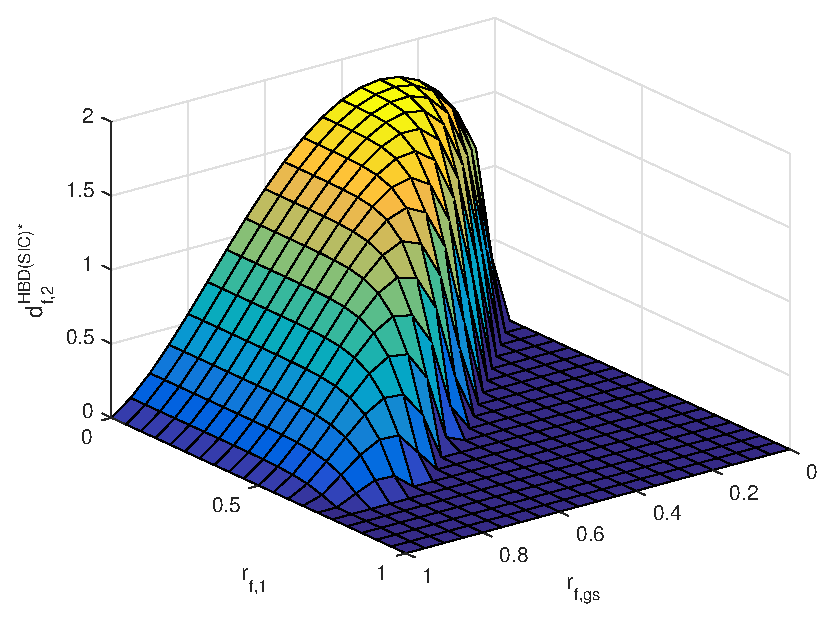
\includegraphics [width=0.45\columnwidth]{chap4_fig/var_df_uav2_sic_surf.eps}
\label{fig:JD_HBD_UCS_var_df_uav2_sic_surf}}
\hfil
\subfloat[Joint detector.]{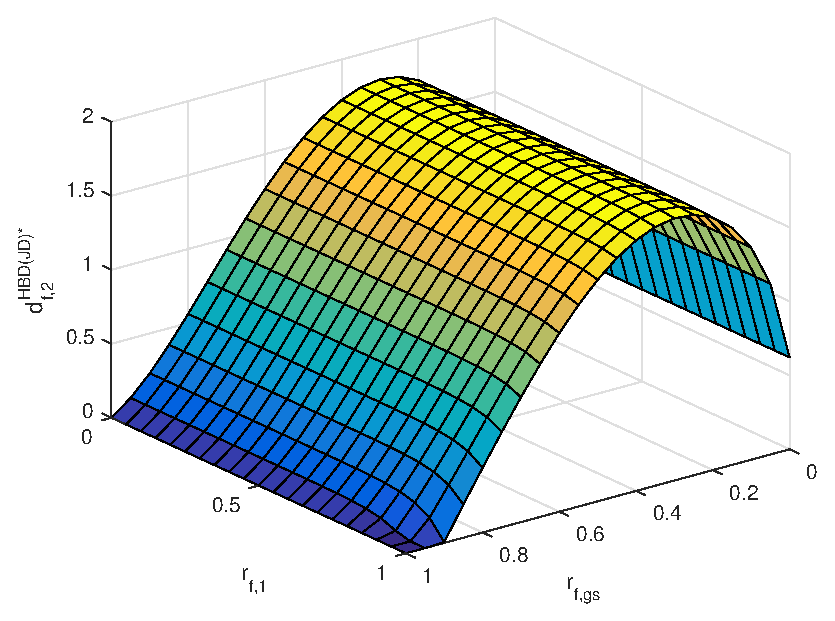
\includegraphics [width=0.45\columnwidth]{chap4_fig/var_df_uav2_jd_surf.eps}
\label{fig:JD_HBD_UCS_var_df_uav2_jd_surf}}
\caption{Achievable finite SNR diversity gain of the SIC detector and joint detector at UAV-2 for different multiplexing gains at UAV-1 ($r_{f,1}$) and the GS ($r_{f,gs}$) when $\alpha_{g,2}=1$, $\alpha_{1,2}=15$ and $\Omega_X=10dB$.}
\label{fig:JD_HBD_UCS_var_mgr_surf_uav2}
%\vspace{-0.5cm}
\end{figure*}

%%%%%%%%%%%%%%%%%%%%%%%%%%%%%%%%%%%%%%%%%%%%%%%%%%%%%%%%%%%%%%%%%
% The SIC detector achieves non-zero diversity gain when the multiplexing gain of the SOI is larger than the multiplexing gain of the interferer. 
% On the contrary, the achievable diversity gain of the joint detector is independent of the multiplexing gain of the interferer.
%%%%%%%%%%%%%%%%%%%%%%%%%%%%%%%%%%%%%%%%%%%%%%%%%%%%%%%%%%%%%%%%%

\begin{figure*}[]
\centering
\subfloat[II and joint detector, $\alpha_{1,2}=0.1$.]{\includegraphics [width=0.45\columnwidth]{chap4_fig/var_df_uav2_jd_ii_mgr_annot2.eps}
\label{fig:JD_HBD_UCS_var_df_uav2_jd_ii_mgr_annot}}
\hfil
\subfloat[SIC and joint detector, $\alpha_{1,2}=15$.]{\includegraphics [width=0.45\columnwidth]{chap4_fig/var_df_uav2_jd_sic_mgr_annot2.eps}
\label{fig:JD_HBD_UCS_var_df_uav2_jd_sic_mgr_annot}}
\caption{Overlapping finite SNR MGRs of the II, SIC and joint detectors at UAV-2 for $\alpha_{g,2}=1$, $\alpha_{1,2}=\{0.1,15\}$ and $\Omega_X=10dB$. (The MGR separation can be smoothen by plotting the regions with very high resolutions.)}
\label{fig:JD_HBD_UCS_var_mgr_uav2}
%\vspace{-0.5cm}
\end{figure*}

%%%%%%%%%%%%%%%%%%%%%%%%%%%%%%%%%%%%%%%%%%%%%%%%%%%%%%%%%%%%%%%%%
% The joint detector achieves non-zero finite SNR diversity gains over a larger MGR region than the II detector, with $d_{f,2}^{HBD(JD)*} > d_{f,2}^{HBD(II)*}$ in $MGR2$.

% Similarly, the joint detector achieves non-zero finite SNR diversity gains over a larger MGR region than the SIC detector. Furthermore, $d_{f,2}^{HBD(JD)*} > d_{f,2}^{HBD(SIC)*}$ in $MGR2$. However, $d_{f,2}^{HBD(JD)*} = d_{f,2}^{HBD(II)*}$ in $MGR3$ when $r_{f,gs}$ is high and $r_{f,1}$ is low since the SIC detector is more likely to detect and remove $x_{1}[t]$.

% As inter-UAV interference increases, the joint detector can achieve non-zero diversity gain over a large MGR. In other words, the interfering signal can be transmitted at higher data rates as inter-UAV interference increases. 
%%%%%%%%%%%%%%%%%%%%%%%%%%%%%%%%%%%%%%%%%%%%%%%%%%%%%%%%%%%%%%%%%

So far, we have assumed that the multiplexing gains of the FD-enabled GS and UAV-1 are the same, i.e., $r_{f,1}=r_{f,gs}=r_f$. In contrast, we assume different multiplexing gains for UAV-1 and the GS in the subsequent analysis. The achievable finite SNR diversity gains for the SIC detector $\big(d_{f,2}^{HBD(SIC)*}\big)$ and the joint detector $\big(d_{f,2}^{HBD(JD)*}\big)$ are plotted in Fig. \ref{fig:JD_HBD_UCS_var_df_uav2_sic_surf} and Fig. \ref{fig:JD_HBD_UCS_var_df_uav2_jd_surf}, respectively. We omit plotting the achievable finite SNR diversity gain of the II detector $\big(d_{f,2}^{HBD(II)*}\big)$ as the expression is independent of the multiplexing gain of the interference ($r_{f,1}$).

\begin{observation}
\emph{\emph{The SIC detector achieves non-zero diversity gain when the multiplexing gain of the SOI is larger than the multiplexing gain of the interferer. On the contrary, the achievable diversity gain of the joint detector is independent of the multiplexing gain of the interferer.}
}\end{observation}

From Fig. \ref{fig:JD_HBD_UCS_var_mgr_surf_uav2}, it is observed that the SIC detector achieves non-zero diversity gain when the multiplexing gain of the SOI is larger than the multiplexing gain of the interferer. As noted in \cite{narasimhan2006finite}, the multiplexing gain of a variable transmission rate scheme determines the impact of Rician $K$ factors on outage decay. In particular, a higher multiplexing gain elicits a stronger influencing effect of the Rician $K$ factor on outage decay and vice versa. The same principle also explains the trend seen in Fig. \ref{fig:JD_HBD_UCS_var_df_uav2_sic_surf} for the SIC detector. As $r_{f,1}$ increases, the Rician $K$ factor corresponding to the interfering link ($K_{Y_1}$) starts to affect the overall outage decay of the SIC detector. Therefore, $r_{f,gs}$ must also increase , i.e., $0<r_{f,1}<r_{f,gs}<1$ to offset the influence of $K_{Y_1}$ on the overall outage decay with the Rician $K$ factor corresponding to the SOI link ($K_{X_{gs}}$).

On the contrary, Fig. \ref{fig:JD_HBD_UCS_var_df_uav2_jd_surf} shows that the achievable diversity gain of the joint detector is independent of the multiplexing gain of the interferer. Therefore, non-zero $d_{f,2}^{HBD(JD)*}$ can be obtained for a wider range of $r_{f,1}$ and $r_{f,gs}$ values compared to the SIC detector. In strong inter-UAV interference scenarios, the joint detector enables the proposed HBD-UCS to accommodate a wider range of data rate requirements compared to the SIC detector. For instance, video streaming capabilities can be deployed on UAV-1 while still meeting the QoS requirements of CNPC links at the FD-enabled GS, even when inter-UAV interference is strong. Hence JD-based HBD-UCS deployment in UAV networks is attractive when the high data rate requirements are met, albeit at the cost of higher computational complexity compared to SIC-based HBD-UCS\footnote{The complexity of the joint detector depends on the particular encoding scheme (e.g., Low-density parity-check or turbo codes) and decoding scheme (e.g., bipartite graph-based or trellis-based decoders), interested readers can refer to \cite{shubhi2017joint} for more details}.
 \newpage
\begin{observation}
\emph{\emph{The joint detector achieves non-zero diversity gain over a larger multiplexing gain region than the II and the SIC detectors under equivalent inter-UAV interference levels.}
}\end{observation}

In Fig. \ref{fig:JD_HBD_UCS_var_df_uav2_jd_ii_mgr_annot}, the MGRs of the joint detector and II detector are shown for $\alpha_{1,2}=0.1$. In particular, the joint detector achieves non-zero $d_{f,2}^{HBD(JD)*}$ in regions $MGR2$ and $MGR3$ while the II detector achieves non-zero $d_{f,2}^{HBD(II)*}$ in regions $MGR1$ and $MGR2$. In $MGR4$, both the joint detector and II detector achieve zero finite SNR diversity gains. Evidently, the joint detector achieves non-zero finite SNR diversity gains over a larger MGR region than the II detector, with $d_{f,2}^{HBD(JD)*} > d_{f,2}^{HBD(II)*}$ in $MGR2$.

In Fig. \ref{fig:JD_HBD_UCS_var_df_uav2_jd_sic_mgr_annot}, the MGRs of the joint detector and SIC detector are shown for $\alpha_{1,2}=15$. The joint detector achieves non-zero $d_{f,2}^{HBD(JD)*}$ in regions $MGR1$, $MGR2$ and $MGR3$. The SIC detector achieves non-zero $d_{f,2}^{HBD(SIC)*}$ in regions $MGR2$ and $MGR3$. In $MGR4$, both the joint detector and SIC detector achieve zero finite SNR diversity gains. 

From Fig. \ref{fig:JD_HBD_UCS_var_df_uav2_jd_sic_mgr_annot}, it can be observed that the joint detector achieves non-zero finite SNR diversity gains over a larger MGR region than the SIC detector. Furthermore, $d_{f,2}^{HBD(JD)*} > d_{f,2}^{HBD(SIC)*}$ in $MGR2$. However, $d_{f,2}^{HBD(JD)*} = d_{f,2}^{HBD(II)*}$ in $MGR3$ when $r_{f,gs}$ is high and $r_{f,1}$ is low since the SIC detector is more likely to detect and remove $x_{1}[t]$. As inter-UAV interference increases, the joint detector can achieve non-zero diversity gain over a large MGR. In other words, the interfering signal can be transmitted at higher data rates as inter-UAV interference increases. 

The trends in Fig. \ref{fig:JD_HBD_UCS_var_mgr_surf_uav2} and Fig. \ref{fig:JD_HBD_UCS_var_mgr_uav2} show that the joint detector enables the proposed HBD-UCS to achieve higher reliability than the II and SIC detectors while meeting a wider range of QoS requirements. Therefore, the JD-based HBD-UCS is more flexible in responding to changing QoS requirements and exhibits better reliability over II-based and SIC-based HBD-UCS in multi-UAV networks.

%%%%%%%%%%%%%%%%%%%%%%%%%%%%%%%%%%%%%%%%%%%%%%%%%%%%%%%%%%%%%%%%%%%%%%%%%%%%%%%%%%%%%%%%%%%%%%%%%%%%%%%%%%%%%%%%%%%%%%%%%%%%%%%%%%%%%%%%%
% Section: Conclusion
\section{Chapter Summary}
An HBD-UCS with JD is proposed in this chapter as a step towards addressing spectrum scarcity in UAV communications. An innovative approach to deriving closed-form outage probability and finite SNR diversity gain expressions over Rician fading channels is also presented. Through a comprehensive performance analysis, suitable detectors for various inter-UAV interference scenarios are identified. The degree of performance improvements offered by the joint detector over the II and the SIC detectors are also highlighted. It is also observed that the SIC detector achieves non-zero diversity gain when the interfering signal from UAV-1 is transmitted at a lower data rate than the SOI from the FD-enabled GS. However, when inter-UAV interference is sufficiently strong, the joint detector is observed to be independent of the data rate of the interfering signal. An analysis of the MGR for the II, SIC, and the joint detectors is also conducted, where it is shown that the JD-based HBD-UCS can support a wide range of data rate requirements while achieving superior reliability over the II-based and SIC-based HBD-UCS. 

% Work is in progress on evaluating the JD-based HBD-UCS against II-based HBD-UCS, SIC-based HBD-UCS and HD-UCS through stochastic geometry framework. In addition, the impact of Rician $K$ factors on HBD-UCS performance, extending the outage and finite SNR analysis framework for combinations of Rician and Rayleigh fading with imperfect channel estimation, the design of robust and low complexity SIC detectors and joint detectors that considers multiple UAVs and FD-enabled GSs, and beamforming solutions are also being investigated as part of future works.

While II-based, SIC-based, and JD-based HBD-UCSs has been shown to be highly effective for UAV communications over Rician fading channels, the performance of joint detection over channels experiencing joint fading and shadowing is unclear. Thus, in the next chapter, the performance of the HBD-UCS is evaluated in a Rician shadowed fading environment to understand the effects of fading and shadowing on UAV communications.



%---------------------------------------------------------------------------------
\chapter{Hybrid-Duplex UAV Communication in Rician Shadowed Fading Environments}
\label{chap:HBD_UCS_Rician_Shadowed}
%---------------------------------------------------------------------------------
\section{Introduction}

In Chapter \ref{chap:JD_HBD_UCS}, the performance of II-based, SIC-based, and JD-based HBD-UCSs operating in Rician fading environments was studied as a potential solution to address spectrum scarcity in UAV communications. Although Rician fading channels are commonly encountered in UAV communications, transmissions in practice are also impaired by the combined effect of fading and shadowing \cite{matolak2015unmannedAircraft,matolak2012air}, especially in urban environments \cite{al2014optimal}.\footnote{The work in this chapter has been published in \cite{ernest2019power}.}

To begin modeling a realistic UAV communication channel, it is first noted that channel measurement campaigns for UAV-to-ground links showed a \textcolor{black}{close match between the measurement data and the Rician fading model \cite{sun2017air_hilly}}. For UAV-to-UAV links, i.e., inter-UAV channels, measurement campaigns in \cite{goddemeier2015investigation} have also demonstrated the Rician fading channel as a suitable model for inter-UAV links. \textcolor{black}{The authors in \cite{yuan2018capacity} similarly employ} the Rician fading model for inter-UAV links to account for the availability of LOS links, scattering, and reflection from the environment. Nonetheless, despite several recent works on UAV channel modeling, e.g., \cite{zeng20173d,jin2017three,jiang2019three,jiang2018three}, channel models that jointly account for fading and shadowing have not been investigated extensively. In particular, the Rician fading model may not be accurate in a suburban environment as it does not account for shadowing due to terrain or buildings \cite{matolak2015unmannedAircraft,matolak2012air,al2014optimal}. In the empirical data of \cite{sun2017air_hilly}, where the characterization of UAV communication channels in hilly terrain was studied, Rician shadowed fading, i.e., LOS blockage, was observed. However, due to the limited dynamic range of the transceiver used during the measurement campaign, the authors in \cite{sun2017air_hilly} omitted measurement data containing LOS shadowing.

In light of the above limitations, the Rician shadowed fading model presented in \cite{tan2018ricianShad} is a suitable choice for UAV channel modeling. Through the Rician shadowed fading model, Rician fading or Rayleigh fading UAV channels \cite{ernest2018hybrid} can be modeled as special cases. It is worth noting that the Rician shadowed fading model is one of several shadowed fading, i.e., composite fading, models available in the literature. \textcolor{black}{Such composite fading models combine shadowing, i.e., large-scale fading, with small-scale fading, e.g., $\kappa - \mu$ or Rician fading\footnote{Small-scale fading occurs when the received signal power undergoes variations due to LOS or NLOS components, multipath clustering with circularly symmetric or elliptical scattering, and power imbalance between the in-phase and quadrature signal components \cite{chun2017comprehensive}. Depending on the type of environment, different kinds of small-scale fading can occur. For instance, Rician fading is commonly encountered in UAV communications \cite{matolak2017air_suburban}, \cite{sun2017air_hilly}, which can be modeled using the non-centered Chi-squared distribution.}. Also, fluctuations caused by shadowing are modeled using Gaussian, lognormal, gamma, or inverse Gaussian distributions \cite{al2014optimal,chun2017comprehensive}}.\footnote{Shadowing occurs when a communication link is obstructed by buildings or terrain \cite{matolak2015unmannedAircraft, matolak2012air, al2014optimal, chun2017comprehensive}, causing the total received signal power to fluctuate randomly \cite{chun2017comprehensive}. The resultant fluctuations can be modeled using the Gaussian, lognormal, gamma, or inverse Gaussian distributions \cite{al2014optimal, chun2017comprehensive}.} For the Rician shadowed fading model, one can employ the $\kappa - \mu$ shadowed fading model, where the non-centered Chi-squared and Nakagami-$m$ distributions are assumed for the multipath and LOS components, respectively \cite{chun2017comprehensive,paris2014statistical,zhang2017high,li2017effective}. In particular, the non-centered Chi-squared distribution accounts for both the LOS and NLOS components encountered over the UAV channel, while the degree of LOS shadowing is modeled through the Nakagami-$m$ distribution. Thus, using the Rician shadowed fading model, the severity of LOS shadowing and the ratio of the LOS-to-NLOS components can be accurately captured through the Nakagami-$m$ shaping parameter and the Rician $K$ factor, respectively. Furthermore, in contrast to the $\kappa - \mu$ shadowed fading model which considers LOS and NLOS shadowing for more than one multipath cluster, only one multipath cluster with LOS shadowing is considered for the Rician shadowed fading model. On top of the Rician shadowed fading model, it was shown by Paris \cite{paris2014statistical} that the $\kappa - \mu$ shadowed fading model includes the one-sided Gaussian, Rayleigh, $\kappa - \mu$, and Rician fading models as special cases, obtainable through the substitution of appropriate shaping parameters. However, the relevant statistics from \cite{chun2017comprehensive} and \cite{paris2014statistical} are represented in the form of complicated functions, such as the confluent hypergeometric function \cite{gradshteyn2014table} and the Gauss hypergeometric function \cite{kumar2015approximate}, which may not yield tractable solutions. \textcolor{black}{Hence}, one can adopt the Rician shadowed fading model presented in \cite{tan2018ricianShad}. In particular, the work in \cite{tan2018ricianShad} presented power series expressions for statistics in the Rician shadowed fading model. While the closed-form expressions in  \cite{tan2018ricianShad} enables tractable mathematical analysis, the generality of the Rician shadowed fading model using the power series approach, i.e., to obtain the Rician fading model, remains an open research problem which will be investigated in this chapter.

Although UAV communications in the presence of shadowing has been studied in the literature, e.g., \cite{motlagh2016uav,al2017modeling,amorim2017radio}, these works have not considered Rician shadowed fading or Rician fading and are only valid for interference-free scenarios. For interference management strategies, the II approach has already been investigated from the outage probability perspective for aeronautical communications over Rician fading channels \cite{ernest2019outage,ernest2018performance}, and for UAV communications over Rician fading channels \cite{ernest2018hybrid} and Rician shadowed fading channels \cite{tan2018ricianShad}. In particular, the work in \cite{tan2018ricianShad} presented new power series expressions for statistics associated with the Rician shadowed fading model. Thereafter, closed-form outage probability expressions for the II detector involving SINRs of the form $\frac{Z_0}{1+Z_1}$, where $Z_0$ and $Z_1$ denote the desired and interfering signals, respectively, were derived for the Rician shadowed fading model through a power series approach. Thus, through the power series approach in \cite{tan2018ricianShad}, one can easily obtain closed-form outage probability expressions for the II detector over Rician shadowed fading channels. In contrast, one may have to resort to numerical methods to evaluate the outage probability of the II detector using the statistics presented in \cite[eq. (3)]{abdi2003new}, \cite[eq. (12)]{chun2017comprehensive}, and \cite[eq. (4)]{paris2014statistical}. For the JD strategy, closed-form outage probability expressions are only available for Rician fading channels, e.g., \cite{tan2018joint}. Therefore, the outage probability analysis of UAV communications for JD over Rician shadowed fading channels through closed-form expressions remains an open problem.

To this end, we extend the Rician shadowed fading model in \cite{tan2018ricianShad} to include the Rician fading model as a special case. It is worth mentioning that closed-form power series expressions for the Rician fading model are already available in \cite[Table I and Table II]{rached2017unified}. However, we present alternative power series representations for the Rician fading model using the Rician shadowed fading model in this chapter. \textcolor{black}{We} demonstrate that the Rician shadowed fading model in this chapter unifies Rician shadowed fading, Rician fading, and Rayleigh fading under the same power series-based model. Through the newly obtained closed-form expressions for the Rician shadowed fading model, we conduct an outage probability analysis of HBD UAV communications for multi-UAV networks in both Rician shadowed fading and Rician fading environments. Specifically, the outage probability analysis takes into consideration the effects of inter-UAV interference, SI, fading, and shadowing for the II and JD interference management approaches. Additionally, it is worth noting that this chapter is an extension of the work in \cite{tan2018ricianShad}, where the UAV-to-GS and the SI links are modeled as Rician fading channels. \textcolor{black}{The} current chapter models the UAV channels and SI channel using the Rician shadowed fading model. As such, the system model and the subsequent analysis in \cite{tan2018ricianShad} can be obtained in this chapter as specific cases, thus illustrating the generality of the employed Rician shadowed fading model in this chapter. 

%Thus, the main contributions of this paper are summarized below.
%
%% Major contributions
%\subsection{Main Contributions}
%\begin{itemize}
%\item The present paper proposes a novel approach towards obtaining alternative power series representations of the probability density function (PDF), cumulative distribution function (CDF), and fractional moment for both the Rician fading and the Rician shadowed fading models.
%\item From the derived equations, closed-form outage probability expressions for the II and joint detectors using alternative power series expressions for the Rician shadowed fading and Rician fading models are obtained. To the best of our knowledge, the closed-form outage probability expressions and analysis are unavailable in the literature.
%\item Although counter-intuitive, it is shown that the impact of shadowing on the SI link at the FD-enabled GS is negligible. We also show that severe shadowing on the desired link with strong LOS component, as compared to weak LOS component, causes reduction in reliability even when SI mitigation measures are implemented.
%\item At UAV-2, the effect of severe shadowing on the desired link with strong LOS components is shown to be less severe for the joint detector than for the II detector.
%\end{itemize}
%
%% Organization of the paper
%The remainder of this paper is organized as follows. The system model is introduced in Section \ref{sec_sys_model}, with alternative expressions for both Rician fading and Rician shadowed fading models presented in Section \ref{sec_rician_shad}. Outage probability expressions are presented in Section \ref{sec_outage}, with numerical results discussed in Section \ref{sec_num_res} before the conclusion of the paper in Section \ref{sec_conclusion}.

%%%%%%%%%%%%%%%%%%%%%%%%%%%%%%%%%%%%%%%%%%%%%%%%%%%%%%%%%%%%%%%%%%%%%%%%%%%%%%%%%%%%%%%%%%%%%%%%%%%%%%%%%%%%%%%%%%%%%%%%%%%%%%%%%%%%%%%%%
% Section 2 : System Model
\section{System Model} \label{HBD_UCS_Rician_Shadowed_sec_sys_model}
%\vspace{-1cm}
\begin{figure} [tpb]
\centering
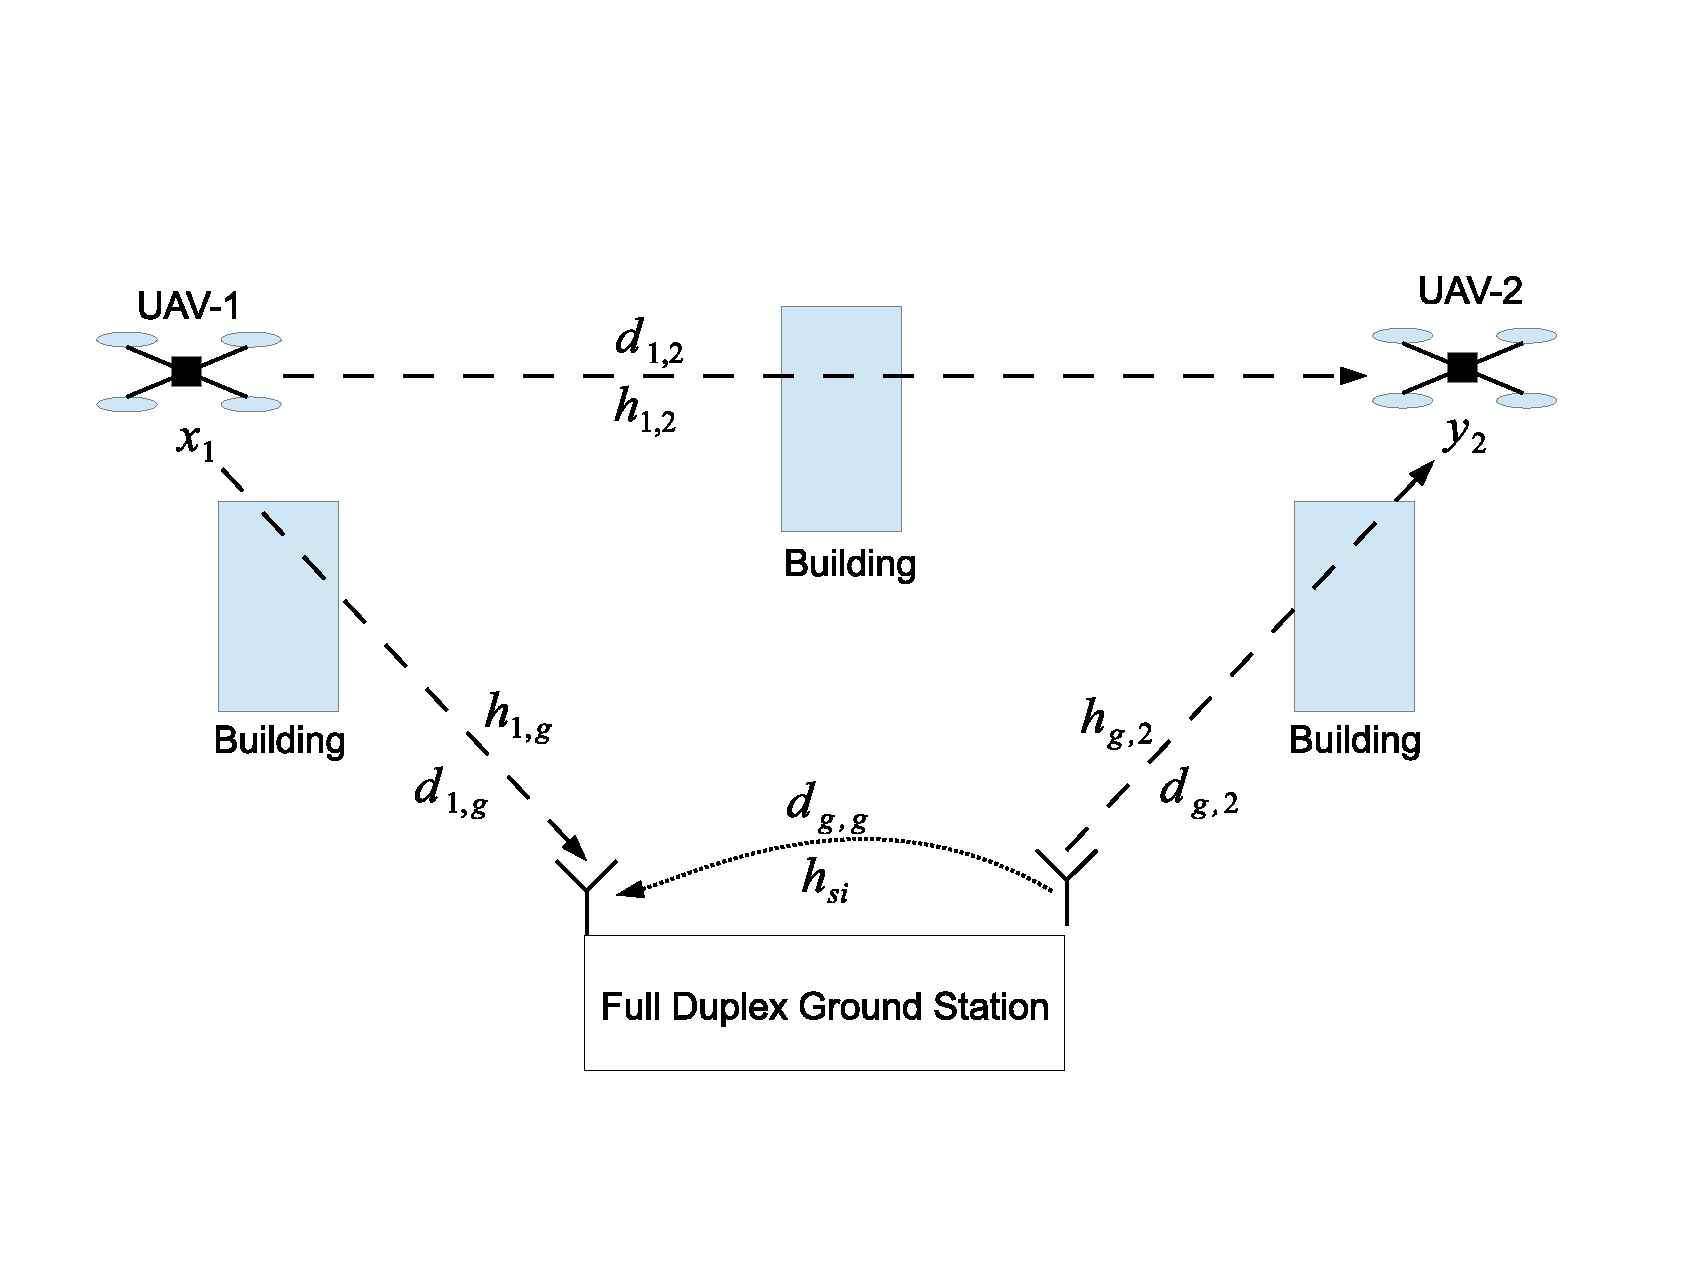
\includegraphics [width=0.5\columnwidth]{chap5_fig/block_diagram.eps}
\vspace{-1cm}
\caption{Unmanned Aerial Vehicle 1 (UAV-1) and Unmanned Aerial Vehicle 2 (UAV-2) operating in HD mode while communicating with the FD GS over Rician shadowed fading channels.}
%\vspace{-1cm}
\label{fig:HBD_UCS_Rician_Shadowed_block_diagram}
%\vspace{-0.3in}
\end{figure}

The multi-UAV HBD-UCS operating in a suburban environment is shown in Fig. \ref{fig:HBD_UCS_Rician_Shadowed_block_diagram}. In particular, it is assumed that the HD UAV-1 is simultaneously transmitting data to the FD-enabled GS while the HD UAV-2 is receiving control information on the same channel (Fig. \ref{fig:HBD_UCS_Rician_Shadowed_block_diagram}). Such an arrangement enables the HBD-UCS to utilize spectrum efficiently, which is a challenge in UAV communications \cite{matolak2017air_suburban}. Another major issue in multi-UAV networks is the interference present in the HBD-UCS \cite{motlagh2016low}. In Fig. \ref{fig:HBD_UCS_Rician_Shadowed_block_diagram}, signals from Unmanned Aerial Vehicle 1 (UAV-1) are transmitted to both GS and Unmanned Aerial Vehicle 2 (UAV-2) as the SOI and interference, respectively. Simultaneously at the FD-enabled GS, signals are transmitted to UAV-2. Consequently, inter-UAV interference and SI are experienced at UAV-2 and the FD-enabled GS, respectively.

In a suburban environment, it is likely \textcolor{black}{that} LOS components to be obstructed by buildings \cite{matolak2015unmannedAircraft,matolak2012air,al2014optimal}. As such, Rician shadowed fading \cite{chun2017comprehensive} is assumed on all UAV links ($h_{1,g}, h_{g,2}, h_{1,2}$) to adequately model the suburban UAV communication channels. As in \cite{tan2018joint}, UAV mobility is assumed to be compensated in this chapter. For SI channel modeling at the FD-enabled GS, recent literature have assumed the Rayleigh fading model \cite{mohammadi2015full,yue2018exploiting,yao2018x} or the Rician fading model \cite{ahmed2015all}. However, in this chapter, the SI link ($h_{si}$) at the FD-enabled GS is modeled as a Rician shadowed fading channel. Such an assumption enables the analysis to consider the effects of passive SI suppression through shadowing experienced on the SI channel. Additionally, Rayleigh fading can be obtained through the Rician shadowed fading model as a special case by letting the Rician $K$ factor be zero. Also, it is assumed that the SI signal undergoes active SI mitigation after passive SI suppression at the FD-enabled GS. Thus, only residual SI is considered at the GS. A summary of important notations is also given in Table \ref{table:HBD_UCS_Rician_Shadowed_summary_impt_notations}.


\subsection{Ground Station}
At the GS, let the SOI transmitted from UAV-1 be $x_1[t]$, the signal transmitted from GS be $x_{gs}[t]$, and the SI be $x_{si}[t]$, where $x_{si}[t]=x_{gs}[t]$. Also, let $h_{1,g}[t]$, $h_{si}$, and $\widetilde{h}_{si}=h_{si}-\widehat{h}_{si}$ be the channel between UAV-1 and GS, the SI channel gain, and the SI channel gain estimate error, respectively, where $\widehat{h}_{si}$ is the imperfect estimation of the SI channel gain. Then, the received signal at GS can be written as \cite{sahai2013impact}:
%%%%%%%%%%%%%%%%%%%%%%%%%%%%%%%%%%%%%%%%%%%%%%%%%%%%%%%%%%%%%%%%%%%%%%%%%%%%%%%%%
\begin{eqnarray} \label{HBD_UCS_Rician_Shadowed_y_gs}
y_{gs}[t] & = & \sqrt{\Omega_{X}}h_{1,g}[t]x_{1}[t] + \sqrt{\Omega_X\alpha_{g,g}}|h_{si}|\gamma_{\phi}w_{\phi}[t] + \sqrt{\Omega_X\alpha_{g,g}} \cdot |\widetilde{h}_{si}|x_{si}[t] + w_{g}[t], 
\end{eqnarray}
%%%%%%%%%%%%%%%%%%%%%%%%%%%%%%%%%%%%%%%%%%%%%%%%%%%%%%%%%%%%%%%%%%%%%%%%%%%%%%%%%
where $w_{g}[t]$ is the AWGN at GS with zero-mean and variance $\sigma_g^2$, and $w_{\phi}[t]$ is the Gaussian distributed phase noise term with zero-mean and unit variance, scaled by phase noise strength $\gamma_{\phi}$ \cite{sahai2013impact}\footnote{The scaling factor $\gamma_{\phi}$ models the jitter present in oscillators due to hardware imperfections \cite{sahai2013impact}}. The imperfect SI channel estimate ($\widetilde{h}_{si}$) is modeled as a circularly symmetric zero-mean complex Gaussian random variable RV with variance $\epsilon$ to model the worst case residual SI \cite{zlatanov2017capacity}.

Using the free space path loss model, the average received signal power of the SOI ($\Omega_{X}$), normalized by $\sigma_g^2$, is defined as:
%%%%%%%%%%%%%%%%%%%%%%%%%%%%%%%%%%%%%%%%%%%%%%%%%%%%%%%%%%%%%%%%%%%%%%%%%%%%%%%%%
\begin{eqnarray} \label{HBD_UCS_Rician_Shadowed_Omega_x_soi}
\Omega_{X} \propto \frac{P_t}{(d_{1,g})^{n}\sigma_g^2}_,
\end{eqnarray}
%%%%%%%%%%%%%%%%%%%%%%%%%%%%%%%%%%%%%%%%%%%%%%%%%%%%%%%%%%%%%%%%%%%%%%%%%%%%%%%%%
where $P_{t}$ and $d_{1,g}$ are the transmit power (Watts) and distance (km), respectively. It should be pointed out that equal transmit power $P_t$ is assumed for the HBD-UCS and $h_{1,g}[t]$ is chosen as the reference link in this chapter. Thus, the average received signal power in the other links are expressed relative to $h_{1,g}[t]$, using the multiplicative factor ($\alpha_{i,j}$) defined as:
%%%%%%%%%%%%%%%%%%%%%%%%%%%%%%%%%%%%%%%%%%%%%%%%%%%%%%%%%%%%%%%%%%%%%%%%%%%%%%%%%
\begin{eqnarray} \label{HBD_UCS_Rician_Shadowed_alpha_i_j}
\alpha_{i,j} = \bigg(\frac{d_{1,g}}{d_{i,j}}\bigg)^n, i\in\left\{g,1\right\}, j\in\left\{g,2\right\}, i \neq j.
\end{eqnarray}
%%%%%%%%%%%%%%%%%%%%%%%%%%%%%%%%%%%%%%%%%%%%%%%%%%%%%%%%%%%%%%%%%%%%%%%%%%%%%%%%%

For $i=j=g$, $\alpha_{g,g}$ is treated as a scaling variable for the average residual SI power at the GS. Together with $\alpha_{g,g}$, $\sigma_g^2$, and $\epsilon$, the amount of SI suppression is quantified as $\frac{1}{\alpha_{g,g}\epsilon\sigma_g^2}$ \cite{ernest2019outage,zlatanov2017capacity}.

\subsection{Unmanned Aerial Vehicle 2}
At UAV-2, let the SOI transmitted from GS be $x_{gs}[t]$, and the inter-UAV interference from UAV-1 be $x_1[t]$. Also, let $h_{g,2}[t]$ and $h_{1,2}[t]$ be the channels between GS and UAV-2, and UAV-1 and UAV-2, respectively. Then, the received signal at UAV-2 can be expressed as:
%%%%%%%%%%%%%%%%%%%%%%%%%%%%%%%%%%%%%%%%%%%%%%%%%%%%%%%%%%%%%%%%%%%%%%%%%%%%%%%%%
\begin{eqnarray} \label{HBD_UCS_Rician_Shadowed_y_uav2}
y_{2}[t] = \sqrt{\Omega_{X}\alpha_{g,2}}h_{g,2}[t]x_{gs}[t] + \sqrt{\Omega_{X}\alpha_{1,2}}h_{1,2}[t]x_{1}[t]  +  w_{2}[t],
\end{eqnarray}
%%%%%%%%%%%%%%%%%%%%%%%%%%%%%%%%%%%%%%%%%%%%%%%%%%%%%%%%%%%%%%%%%%%%%%%%%%%%%%%%%
where $w_{2}[t]$ is the AWGN at UAV-2 with zero-mean and variance $\sigma_2^2$. Additionally, $\Omega_{X}\alpha_{g,2}$ and $\Omega_{X}\alpha_{1,2}$ respectively indicate the average received signal powers of the SOI and interfering signal. Due to the presence of interference at both the FD-enabled GS and UAV-2, II and JD interference management approaches are considered in this chapter.

\begin{table}[]
\centering
\caption{Summary of Important Notations}
\label{table:HBD_UCS_Rician_Shadowed_summary_impt_notations} 
\scalebox{0.8}{
\begin{tabular}{ll}
\hline
\textbf{Notations}		& \textbf{Description}																			\\  \hline \hline
$\Omega_X$						& Average received power																		\\
$\alpha_{i,j}, i\in\left\{g,1\right\}, j\in\left\{g,2\right\}, i \neq j$ & Strength of interference between $i$ and $j$				\\
$\epsilon$						& SI channel estimation error	at the FD-enabled GS					\\
$\gamma_{\phi}^2$			& Strength of phase noise at the FD- enabled GS oscillator	\\
$\sigma_g^2$					& Strength of AWGN at the FD-enabled GS											\\ 
$\sigma_2^2$					& Strength of AWGN at the UAV-2															\\ \hline
\end{tabular}}
\end{table}
%A summary of important notations is also given in Table \ref{table:HBD_UCS_Rician_Shadowed_summary_impt_notations}.

%%%%%%%%%%%%%%%%%%%%%%%%%%%%%%%%%%%%%%%%%%%%%%%%%%%%%%%%%%%%%%%%%%%%%%%%%%%%%%%%%%%%%%%%%%%%%%%%%%%%%%%%%%%%%%%%%%%%%%%%%%%%%%%%%%%%%%%%%
% Section 3 : Shadowed Rician Fading
\section{Alternative Expressions for the Rician Shadowed Fading Model} \label{HBD_UCS_Rician_Shadowed_sec_rician_shad}
% Shadowed Rician fading can be obtained from shadowed k-u fading
The $\kappa-\mu$ shadowed fading model has $\kappa$, $\mu$ and $m$ as shaping parameters \cite{chun2017comprehensive}. Specifically, $\kappa$ represents the ratio between the total powers of the dominant component to the scattered component while $\mu$ denotes the number of multipath clusters. The variable $m$ denotes the shadowing severity, obtained through the Nakagami-m distribution \cite{chun2017comprehensive}. 

For a Rician shadowed fading channel $h$, the channel gain $|h|^2$ is obtained by setting $\mu=1$ and letting $\kappa$ be the Rician $K$ factor \cite{chun2017comprehensive,paris2014statistical}, i.e., $\kappa = K$, as follows \cite[eq. (8)]{chun2017comprehensive}:
%%%%%%%%%%%%%%%%%%%%%%%%%%%%%%%%%%%%%%%%%%%%%%%%%%%%%%%%%%%%%%%%%%%%%%%%%%%%%%%%%
\begin{eqnarray} \label{HBD_UCS_Rician_Shadowed_rician_shad_channel}
|h|^2 = \big[X + {\xi}p\big]^2 + Y^2,
\end{eqnarray}
%%%%%%%%%%%%%%%%%%%%%%%%%%%%%%%%%%%%%%%%%%%%%%%%%%%%%%%%%%%%%%%%%%%%%%%%%%%%%%%%%
where $p = \sqrt{\frac{K}{1+K}}$, $X$ and $Y$ are mutually independent Gaussian RVs with
%%%%%%%%%%%%%%%%%%%%%%%%%%%%%%%%%%%%%%%%%%%%%%%%%%%%%%%%%%%%%%%%%%%%%%%%%%%%%%%%%
\begin{eqnarray}
E\{X\}=E\{Y\} = 0, E\{X^2\}=E\{Y^2\} = \sigma^2,
\end{eqnarray}
%%%%%%%%%%%%%%%%%%%%%%%%%%%%%%%%%%%%%%%%%%%%%%%%%%%%%%%%%%%%%%%%%%%%%%%%%%%%%%%%%
and $\xi$ is a Nakagami-m RV with $E\{\xi^2\}=1$. The term $\big[X + {\xi}p\big]^2$ represents the dominant component and it contains both scattering and LOS components that are subjected to shadowing, while $Y^2$ represents the non-dominant component and it contains only the scattered component \cite{yuan2018capacity}. Additionally, under the obtained Rician shadowed fading model, LOS shadowing is modeled using $\xi$, with $m$ indicating the severity of the shadowing \cite{chun2017comprehensive}. From (\ref{HBD_UCS_Rician_Shadowed_rician_shad_channel}), the PDF of $|h|^2$, i.e., Rician shadowed fading PDF, can be obtained from \cite[Table I]{chun2017comprehensive} as:
%%%%%%%%%%%%%%%%%%%%%%%%%%%%%%%%%%%%%%%%%%%%%%%%%%%%%%%%%%%%%%%%%%%%%%%%%%%%%%%%%
\begin{eqnarray} \label{HBD_UCS_Rician_Shadowed_rician_shad_pdf}
f_{|h|^2}(x) & = & \frac{m^m (1+K)}{\Omega(K+m)^m}\exp\Big(\frac{-(1+K)x}{\Omega}\Big) {}_1F_1\Big(m;1;\frac{K(1+K)}{(K+m)\Omega}x\Big)_,
\end{eqnarray}
%%%%%%%%%%%%%%%%%%%%%%%%%%%%%%%%%%%%%%%%%%%%%%%%%%%%%%%%%%%%%%%%%%%%%%%%%%%%%%%%%
where $\Omega$ and ${}_1{F_1}(\bullet)$ are the average received power and the confluent Hypergeometric function \cite{gradshteyn2014table}, respectively. 

\textcolor{black}{As complicated functions are employed in the above PDF expression, an outage probability analysis of the HBD-UCS may lead to intractable expressions. Separately, it should be noted that the $\kappa - \mu$ shadowed fading model includes the Rician fading and the Rician shadowed fading models as specific cases as it is possible to obtain the Rician fading model from \cite[Table I]{chun2017comprehensive}}. However, in its current form, important performance metrics, e.g., outage probability or finite SNR diversity gain, are not easily obtainable from (\ref{HBD_UCS_Rician_Shadowed_rician_shad_pdf}). Therefore, we present alternative closed-form expressions for the Rician shadowed fading and the Rician fading models in the subsequent sections based on the work in \cite{tan2018ricianShad}.

\subsection{Rician Shadowed Fading Model}

\begin{figure} [t]
\centering
\vspace{0.2cm}
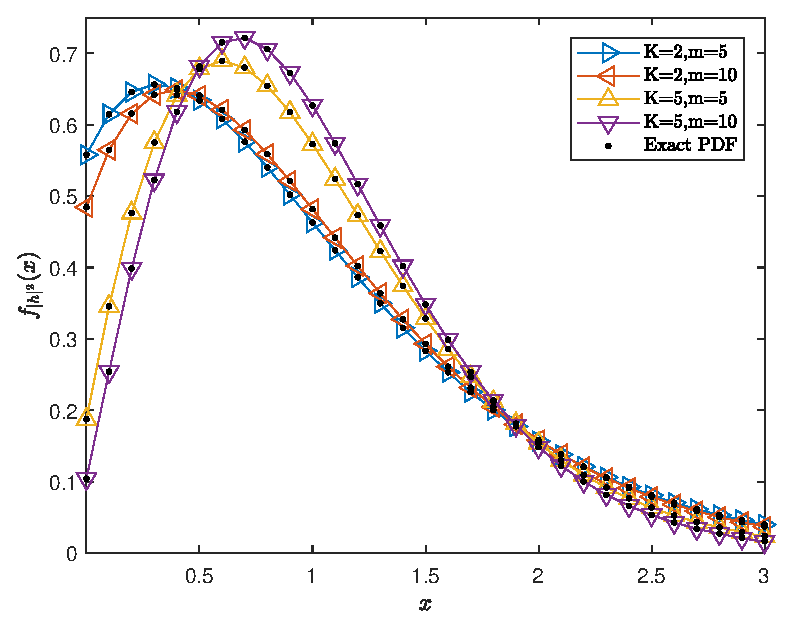
\includegraphics [width=0.45\columnwidth]{chap5_fig/pdf_comparison.eps} 
%\vspace{-0.5cm}
\caption{Comparison between the exact PDF of $|h|^2$ and power series approximation equivalent for $\Omega=1$ and $K_{tr}=50$.}
%\vspace{-0.2cm}
\label{fig:HBD_UCS_Rician_Shadowed_pdf_comparison}
\end{figure}

Let $\overline{a}\big(n,\Omega,K,m,\gamma\big)$ be defined as:
%%%%%%%%%%%%%%%%%%%%%%%%%%%%%%%%%%%%%%%%%%%%%%%%%%%%%%%%%%%%%%%%%%%%%%%%%%%%%%%%%
\begin{eqnarray} \label{HBD_UCS_Rician_Shadowed_rician_shad_cdf_exp}
\overline{a}\big(n,\Omega,K,m,\gamma\big) = \sum_{i=0}^n (-1)^{n-i} \bigg(\frac{m}{K+m}\bigg)^{m} \frac{(m)_i}{\Gamma^2(i+1)} \bigg(\frac{K}{K+m}\bigg)^{i} \bigg(\frac{1+K}{\Omega}\bigg)^{n+1} \frac{\gamma^{n+1}}{(n-i)!(n+1)}_.
\end{eqnarray}
%%%%%%%%%%%%%%%%%%%%%%%%%%%%%%%%%%%%%%%%%%%%%%%%%%%%%%%%%%%%%%%%%%%%%%%%%%%%%%%%%
Then, alternative power series representations of the Rician shadowed fading PDF and the corresponding CDF are presented as follows.

\begin{theorem} \label{HBD_UCS_Rician_Shadowed_pdf_theorem}
The PDF of $|h|^2$ can be represented as the following power series:
%%%%%%%%%%%%%%%%%%%%%%%%%%%%%%%%%%%%%%%%%%%%%%%%%%%%%%%%%%%%%%%%%%%%%%%%%%%%%%%%%
\begin{eqnarray} \label{HBD_UCS_Rician_Shadowed_rician_shad_pdf_pwr_srs}
f_{|h|^2}(x) \approx \sum_{n=0}^{K_{tr}} \overline{a}\big(n,\Omega,K,m,1\big)(n+1)x^n,
\end{eqnarray}
%%%%%%%%%%%%%%%%%%%%%%%%%%%%%%%%%%%%%%%%%%%%%%%%%%%%%%%%%%%%%%%%%%%%%%%%%%%%%%%%%
where $K_{tr}$ denotes the truncation order.
\end{theorem}
\begin{proof} 
The proof can be found in \cite{tan2018ricianShad} and is reproduced in Appendix \ref{HBD_UCS_Rician_Shadowed_pdf_theorem_proof}.
\end{proof}

\begin{theorem} \label{HBD_UCS_Rician_Shadowed_cdf_theorem}
The CDF of $|h|^2$ can be expressed as the following power series: 
%%%%%%%%%%%%%%%%%%%%%%%%%%%%%%%%%%%%%%%%%%%%%%%%%%%%%%%%%%%%%%%%%%%%%%%%%%%%%%%%%
\begin{eqnarray} \label{HBD_UCS_Rician_Shadowed_rician_shad_cdf_pwr_srs}
F_{|h|^2}(\gamma) = \int^{\gamma}_0 f_{|h|^2}(x) dx  \approx  \sum_{n=0}^{K_{tr}} \overline{a}\big(n,\Omega,K,m,\gamma\big)_.
\end{eqnarray}
%%%%%%%%%%%%%%%%%%%%%%%%%%%%%%%%%%%%%%%%%%%%%%%%%%%%%%%%%%%%%%%%%%%%%%%%%%%%%%%%%
\end{theorem}
\begin{proof}
The CDF is obtained by interchanging the summation and integration, i.e., term-wise integration \cite{gradshteyn2014table}.
\end{proof}

\begin{theorem} \label{HBD_UCS_Rician_Shadowed_l_moment_theorem}
The $l^{th}$ moment of $|h|^2$ is given as \cite[eq. (10)]{chun2017comprehensive}:
%%%%%%%%%%%%%%%%%%%%%%%%%%%%%%%%%%%%%%%%%%%%%%%%%%%%%%%%%%%%%%%%%%%%%%%%%%%%%%%%%
\begin{eqnarray} \label{HBD_UCS_Rician_Shadowed_rician_shad_frac_moment}
E\big\{\big(|h|^2\big)^l\big\} & = & \bigg(\frac{\Omega}{1+K}\bigg)^l \Gamma(1+l) \bigg(\frac{m}{K+m}\bigg)^{m-1-l} {}_2F_1\bigg(1-m,1+l;1;\frac{-K}{m}\bigg)_,
\end{eqnarray}
%%%%%%%%%%%%%%%%%%%%%%%%%%%%%%%%%%%%%%%%%%%%%%%%%%%%%%%%%%%%%%%%%%%%%%%%%%%%%%%%%
where $_2F_1(\bullet)$ is the Gauss hypergeometric function \cite{kumar2015approximate}. 
\end{theorem}

Fig. \ref{fig:HBD_UCS_Rician_Shadowed_pdf_comparison} shows the power series representation of $f_{|h|^2}(x)$, computed from (\ref{HBD_UCS_Rician_Shadowed_rician_shad_pdf_pwr_srs}), with the exact PDF in (\ref{HBD_UCS_Rician_Shadowed_rician_shad_pdf}) plotted for comparison. It can be seen that (\ref{HBD_UCS_Rician_Shadowed_rician_shad_pdf_pwr_srs}) provides a close fit to the exact PDF at the cost of computation time, which increases as $m\to\infty$. \textcolor{black}{\footnote{\textcolor{black}{To analytically gauge the accuracy of the new power series expressions, one will need to conduct a truncation analysis. Work in this direction is left as an open research challenge which can be addressed in future studies.}}} Additionally, although not plotted in Fig. \ref{fig:HBD_UCS_Rician_Shadowed_pdf_comparison}, one obtains the Rician fading PDF by letting $m \to \infty$.
 
The closed-form expressions of the PDF, CDF and fractional moments of $|h|^2$, given in (\ref{HBD_UCS_Rician_Shadowed_rician_shad_pdf_pwr_srs}), (\ref{HBD_UCS_Rician_Shadowed_rician_shad_cdf_pwr_srs}), and (\ref{HBD_UCS_Rician_Shadowed_rician_shad_frac_moment}), respectively, are useful in evaluating performance metrics, such as outage probability, in shadowing environments. \textcolor{black}{Furthermore, the new power series expressions for the PDF, CDF and frational moments are, to the best of our knowledge, not available in the literature.}

\subsection{Rician Fading Model}
To understand the impact of shadowing, (\ref{HBD_UCS_Rician_Shadowed_rician_shad_cdf_exp}) and (\ref{HBD_UCS_Rician_Shadowed_rician_shad_frac_moment}) can be evaluated for large values of $m$. In particular, one obtains the Rician fading channel $h^{'}$ from the Rician shadowed fading channel $h$ as $m \to \infty$. In the following Corollaries, new closed-form expressions for Rician fading models are presented.

\begin{corollary} \label{HBD_UCS_Rician_Shadowed_rician_fading_alpha_corollary}
As $m \to \infty$, (\ref{HBD_UCS_Rician_Shadowed_rician_shad_cdf_exp}) can be expressed as:
%%%%%%%%%%%%%%%%%%%%%%%%%%%%%%%%%%%%%%%%%%%%%%%%%%%%%%%%%%%%%%%%%%%%%%%%%%%%%%%%%
\begin{eqnarray} \label{rician_fading_alpha}
\widehat{a}\big(n,\Omega,K,\gamma\big) = \sum_{i=0}^n \frac{(-1)^{n-i} K^i}{\Gamma^2(i+1)} \bigg(\frac{1+K}{\Omega}\bigg)^{n+1} \frac{\exp(-K)\gamma^{n+1}}{(n-i)!(n+1)}_.
\end{eqnarray}
%%%%%%%%%%%%%%%%%%%%%%%%%%%%%%%%%%%%%%%%%%%%%%%%%%%%%%%%%%%%%%%%%%%%%%%%%%%%%%%%%
\end{corollary}
\begin{proof}
The proof can be found in Appendix \ref{HBD_UCS_Rician_Shadowed_rician_fading_alpha_corollary_proof}.
\end{proof}

\begin{remark}
Although not shown in Corollary \ref{HBD_UCS_Rician_Shadowed_rician_fading_alpha_corollary}, it should be noted that \textcolor{black}{the value in }$\widehat{a}\big(n,\Omega,K,\gamma\big)$ in (\ref{rician_fading_alpha}) reduces as $K \to \infty$.
\end{remark}

\begin{corollary} \label{HBD_UCS_Rician_Shadowed_rician_pdf_cdf_corollary}
The PDF $\big(f_{|h^{'}|^2}(\bullet)\big)$ and CDF $\big(F_{|h^{'}|^2}(\bullet)\big)$ of the Rician fading channel $h^{'}$ can be represented as the following power series:
%%%%%%%%%%%%%%%%%%%%%%%%%%%%%%%%%%%%%%%%%%%%%%%%%%%%%%%%%%%%%%%%%%%%%%%%%%%%%%%%%
\begin{eqnarray}
f_{|h^{'}|^2}(x) & \approx & \sum_{n=0}^{K_{tr}} \widehat{a}\big(n,\Omega,K,1\big)(n+1){x^n}_, \label{HBD_UCS_Rician_Shadowed_rician_pdf} \\
F_{|h^{'}|^2}(\gamma) & \approx & \sum_{n=0}^{K_{tr}} \widehat{a}\big(n,\Omega,K,\gamma\big)_, \label{HBD_UCS_Rician_Shadowed_rician_cdf}
\end{eqnarray}
%%%%%%%%%%%%%%%%%%%%%%%%%%%%%%%%%%%%%%%%%%%%%%%%%%%%%%%%%%%%%%%%%%%%%%%%%%%%%%%%%
where $\widehat{a}\big(n,\Omega,K,\gamma\big)$ is given in (\ref{rician_fading_alpha}).
\end{corollary}
\begin{proof}
From (\ref{rician_fading_alpha}), algebraic manipulation yields the power series expression of $f_{|h^{'}|^2}(\bullet)$ and $F_{|h^{'}|^2}(\bullet)$ in (\ref{HBD_UCS_Rician_Shadowed_rician_pdf}) and (\ref{HBD_UCS_Rician_Shadowed_rician_cdf}), respectively.
\end{proof}

\begin{corollary} \label{HBD_UCS_Rician_Shadowed_frac_moments_corollary}
The closed-form expression for the $l^{th}$ moment of $|h^{'}|^2$ is: 
%%%%%%%%%%%%%%%%%%%%%%%%%%%%%%%%%%%%%%%%%%%%%%%%%%%%%%%%%%%%%%%%%%%%%%%%%%%%%%%%%
\begin{eqnarray} \label{HBD_UCS_Rician_Shadowed_frac_moments_corollary_comp_limits}
E\big\{\big(|h^{'}|^2\big)^{l}\big\} = \lim_{m\to\infty}E\big\{\big(|h|^2\big)^l\big\} \approx \bigg(\frac{\Omega}{1+K}\bigg)^l \Gamma(1+l) \sum_{n=0}^{K_{tr}} \frac{(-l)_n}{n!(1)_n}{(-K)^n}_.
\end{eqnarray}
%%%%%%%%%%%%%%%%%%%%%%%%%%%%%%%%%%%%%%%%%%%%%%%%%%%%%%%%%%%%%%%%%%%%%%%%%%%%%%%%%
\end{corollary}
\begin{proof}
The proof can be found in Appendix \ref{HBD_UCS_Rician_Shadowed_frac_moments_corollary_proof}.
\end{proof}

\begin{figure} [t]
\centering
\vspace{0.2cm}
\includegraphics [width=0.45\columnwidth]{chap5_fig/alt_pdf_comparison.eps} 
%\vspace{-0.5cm}
\caption{Comparison between the exact PDF of $|h^{'}|^2$ and power series approximation equivalent for $\Omega=1$ and $K_{tr}=50$.}
%\vspace{-0.2cm}
\label{fig:HBD_UCS_Rician_Shadowed_alt_pdf_comparison}
\end{figure}

\begin{figure} [t]
\centering
\vspace{0.2cm}
\includegraphics [width=0.45\columnwidth]{chap5_fig/alt_cdf_comparison.eps} 
%\vspace{-0.5cm}
\caption{Comparison between the exact CDF of $|h^{'}|^2$ and power series approximation equivalent for $\gamma=0.5$ and $K_{tr}=50$.}
%\vspace{-0.2cm}
\label{fig:HBD_UCS_Rician_Shadowed_alt_cdf_comparison}
\end{figure}

\begin{figure} [t]
\centering
\vspace{0.2cm}
\includegraphics [width=0.45\columnwidth]{chap5_fig/alt_moment_comparison.eps} 
%\vspace{-0.5cm}
\caption{Comparison between the exact fractional moment of $|h^{'}|^2$ and power series approximation equivalent for $\Omega=1$ and $K_{tr}=50$.}
%\vspace{-0.2cm}
\label{fig:HBD_UCS_Rician_Shadowed_alt_moment_comparison}
\end{figure}

The Rician fading PDF in (\ref{HBD_UCS_Rician_Shadowed_rician_pdf}) is plotted in Fig. \ref{fig:HBD_UCS_Rician_Shadowed_alt_pdf_comparison} and compared against the exact Rician fading PDF $f_{|h^{'}|^2}(x) = \frac{K+1}{\Omega} \exp\left(-K-\frac{K+1}{\Omega}x\right)I_{0}\left(2\sqrt{\frac{K(K+1)}{\Omega}x}\right)$, where $I_{0}\left(\cdot\right)$ is the modified Bessel function of the first kind with zero order \cite{gradshteyn2014table}. It can be observed that (\ref{HBD_UCS_Rician_Shadowed_rician_pdf}) provides a close fit to the exact PDF in Fig. \ref{fig:HBD_UCS_Rician_Shadowed_alt_pdf_comparison}. 

The Rician fading CDF $F_{|h^{'}|^2}(\gamma)$ in (\ref{HBD_UCS_Rician_Shadowed_rician_cdf}) is plotted in Fig. \ref{fig:HBD_UCS_Rician_Shadowed_alt_cdf_comparison}. When compared against the numerical integration of $f_{|h^{'}|^2}(x)$ and the exact CDF, $F_{|h^{'}|^2}(\gamma)=1- \\ Q_1\Big( \sqrt{2K}, \sqrt{\frac{2(K+1)\gamma}{\Omega}}\Big)$ where $Q_1\left(\cdot,\cdot\right)$ is the Marcum Q function \cite{rached2017unified}, a close fit is also observed. Similar observations are also made in Fig. \ref{fig:HBD_UCS_Rician_Shadowed_alt_moment_comparison} when (\ref{HBD_UCS_Rician_Shadowed_frac_moments_corollary_comp_limits}) is compared against $E\big\{\big(|h^{'}|^2\big)^l\big\} = \Gamma(1+l) \left[\frac{\Omega}{1+K}\right]^{l} {}_1{F_1}(-l,1;-K)$ \cite[Table II]{rached2017unified}.

Evidently, (\ref{HBD_UCS_Rician_Shadowed_rician_shad_cdf_exp}) and (\ref{HBD_UCS_Rician_Shadowed_rician_shad_frac_moment}) become independent of $m$ as $m \to \infty$. More importantly, Corollaries \ref{HBD_UCS_Rician_Shadowed_rician_fading_alpha_corollary} and \ref{HBD_UCS_Rician_Shadowed_frac_moments_corollary} show that the computed values of (\ref{HBD_UCS_Rician_Shadowed_rician_shad_cdf_exp}) and (\ref{HBD_UCS_Rician_Shadowed_rician_shad_frac_moment}) decreases and increases, respectively, based on the Rician $K$ factor as $m \to \infty$. The presented power series representations of the Rician shadowed fading and Rician fading models in this section are summarized in Table \ref{table:HBD_UCS_Rician_Shadowed_summary_statistics}\footnote{The functions $\gamma(\cdot,\cdot)$, $I_{0}\left(\cdot\right)$, $Q_1\left(\cdot,\cdot\right)$, and ${}_1{F_1}(\bullet)$ represent the lowercase incomplete gamma function \cite{chun2017comprehensive}, the modified Bessel function of the first kind with zero order \cite{gradshteyn2014table}, the Marcum Q function \cite{rached2017unified}, and the confluent Hypergeometric function \cite{gradshteyn2014table}, respectively. The fractional moment of $|h|^2$, i.e., $E\{(|h|^2)^j\}$ is given in (\ref{HBD_UCS_Rician_Shadowed_rician_shad_frac_moment}) while $\overline{a}\big(n,\Omega,K,m,1\big)$ and $\widehat{a}\big(n,\Omega,K,\gamma\big)$ are given in (\ref{HBD_UCS_Rician_Shadowed_rician_shad_cdf_exp}) and (\ref{rician_fading_alpha}), respectively.}. Together, these observations and expressions are essential in evaluating the outage probability of the HBD-UCS, which is discussed in Section \ref{HBD_UCS_Rician_Shadowed_sec_outage}.

%\begin{table*}[]
%\centering
%\caption{Summary of presented closed-form expressions for the Rician shadowed fading and Rician fading models}
%\label{table:HBD_UCS_Rician_Shadowed_summary_statistics}
%\scalebox{0.7}{
%\begin{tabular}{lll}
%\hline
%\textbf{Fading Model}	& \textbf{Expression}																																																											& \textbf{Comment}	\\ \hline \hline
%Rician shadowed (PDF)	& $f_{|h|^2}(x) \approx \sum_{n=0}^{K_{tr}} \overline{a}\big(n,\Omega,K,m,1\big)(n+1)x^n$ 																								& Current Work 							\\
											%& $f_{|h|^2}(x) = \frac{m^m (1+K)}{\Omega(K+m)^m}\exp\Big(\frac{-(1+K)x}{\Omega}\Big){}_1F_1\Big(m;1;\frac{K(1+K)x}{(K+m)\Omega}\Big)$		& \cite{chun2017comprehensive} \\
											%& $f_{|h|^2}(x) = \sum_{n=0}^{\infty} \sum_{i=0}^{n} \sum_{j=0}^{n} \frac{(-1)^{i+j}}{\Gamma[i+1]j!}\binom{n}{i} \binom{n}{n-j} E\{(|h|^2)^j\}x^{i}\exp(-x)$ 																																																																																& \cite{chun2017comprehensive} \\
%Rician shadowed	(CDF)	& $F_{|h|^2}(\gamma) \approx  \sum_{n=0}^{K_{tr}} \overline{a}\big(n,\Omega,K,m,\gamma\big)$ 																							& Current Work 							\\
											%& $F_{|h|^2}(x) = \sum_{n=0}^{\infty} \sum_{i=0}^{n} \sum_{j=0}^{n} \frac{(-1)^{i+j}}{\Gamma(i+2)j!} \binom{n}{i} \binom{n}{n-j} E\{(|h|^2)^j\}x^{i+1} + \gamma(1,x)$ 																																																																															 & \cite{chun2017comprehensive} \\
%Rician (PDF)					& $f_{|h^{'}|^2}(x) \approx \sum_{n=0}^{K_{tr}} \widehat{a}\big(n,\Omega,K,1\big)(n+1)x^n$ 																								& Current Work 							\\
											%&	$f_{|h^{'}|^2}(x) = \frac{K+1}{\Omega} \exp\left(-K-\frac{K+1}{\Omega}x\right)I_{0}\left(2\sqrt{\frac{K(K+1)}{\Omega}x}\right)$ 				& \cite{rached2017unified} 	\\
%Rician (CDF)					& $F_{|h^{'}|^2}(\gamma) \approx \sum_{n=0}^{K_{tr}} \widehat{a}\big(n,\Omega,K,\gamma\big)$ 																							& Current Work 						 	\\ 
											%&	$F_{|h^{'}|^2}(\gamma)=1-Q_1\Big( \sqrt{2K}, \sqrt{\frac{2(K+1)\gamma}{\Omega}}\Big)$ 																									& \cite{rached2017unified} 	\\
%Rician (Fractional Moment)	& $E\big\{\big({|h^{'}|^2}\big)^l\big\} \approx \Big(\frac{\Omega}{1+K}\Big)^l \Gamma(1+l) \sum_{n=0}^{K_{tr}} \frac{(-l)_n}{n!(1)_n}(-K)^n$ & Current Work 					\\
											%&	$E\big\{\big({|h^{'}|^2}\big)^l\big\} = \Gamma(1+l) \left[\frac{\Omega}{1+K}\right]^{l} {}_1{F_1}(-l,1;-K)$ 														& \cite{rached2017unified} 	\\ \hline
%\end{tabular}}
%\end{table*}

\begin{table*}[]
\centering
\caption{Summary of presented closed-form expressions for the Rician shadowed fading and Rician fading models}
\label{table:HBD_UCS_Rician_Shadowed_summary_statistics}
\scalebox{0.8}{
\begin{tabular}{lll}
\hline
\textbf{Fading Model}	& \textbf{PDF Expression}																																																									& \textbf{Comment}	\\ \hline \hline
Rician shadowed 			& $f_{|h|^2}(x) \approx \sum_{n=0}^{K_{tr}} \overline{a}\big(n,\Omega,K,m,1\big)(n+1)x^n$ 																								& Current Work 							\\
											& $f_{|h|^2}(x) = \frac{m^m (1+K)}{\Omega(K+m)^m}\exp\Big(\frac{-(1+K)x}{\Omega}\Big){}_1F_1\Big(m;1;\frac{K(1+K)x}{(K+m)\Omega}\Big)$		& \cite{chun2017comprehensive} \\
											& $f_{|h|^2}(x) = \sum_{n=0}^{\infty} \sum_{i=0}^{n} \sum_{j=0}^{n} \frac{(-1)^{i+j}}{\Gamma[i+1]j!}\binom{n}{i} \binom{n}{n-j} E\{(|h|^2)^j\}x^{i}\exp(-x)$ 																																																																																& \cite{chun2017comprehensive} \\
Rician 								& $f_{|h^{'}|^2}(x) \approx \sum_{n=0}^{K_{tr}} \widehat{a}\big(n,\Omega,K,1\big)(n+1)x^n$ 																								& Current Work 							\\
											&	$f_{|h^{'}|^2}(x) = \frac{K+1}{\Omega} \exp\left(-K-\frac{K+1}{\Omega}x\right)I_{0}\left(2\sqrt{\frac{K(K+1)}{\Omega}x}\right)$ 				& \cite{rached2017unified} 	\\
											&																																																																					& 													\\	\hline
\textbf{Fading Model}	& \textbf{CDF Expression}																																																									& \textbf{Comment}					\\ \hline \hline
Rician shadowed				& $F_{|h|^2}(\gamma) \approx  \sum_{n=0}^{K_{tr}} \overline{a}\big(n,\Omega,K,m,\gamma\big)$ 																							& Current Work 							\\
											& $F_{|h|^2}(x) = \sum_{n=0}^{\infty} \sum_{i=0}^{n} \sum_{j=0}^{n} \frac{(-1)^{i+j}}{\Gamma(i+2)j!} \binom{n}{i} \binom{n}{n-j} E\{(|h|^2)^j\}x^{i+1} + \gamma(1,x)$ 																																																																															 & \cite{chun2017comprehensive} \\
Rician 								& $F_{|h^{'}|^2}(\gamma) \approx \sum_{n=0}^{K_{tr}} \widehat{a}\big(n,\Omega,K,\gamma\big)$ 																							& Current Work 						 	\\ 
											&	$F_{|h^{'}|^2}(\gamma)=1-Q_1\Big( \sqrt{2K}, \sqrt{\frac{2(K+1)\gamma}{\Omega}}\Big)$ 																									& \cite{rached2017unified} 	\\
											&																																																																					&														\\ \hline
\textbf{Fading Model}	& \textbf{Fractional Moments Expression}																																																	& \textbf{Comment}					\\ \hline \hline
Rician 								& $E\big\{\big({|h^{'}|^2}\big)^l\big\} \approx \Big(\frac{\Omega}{1+K}\Big)^l \Gamma(1+l) \sum_{n=0}^{K_{tr}} \frac{(-l)_n}{n!(1)_n}(-K)^n$ & Current Work 					\\
											&	$E\big\{\big({|h^{'}|^2}\big)^l\big\} = \Gamma(1+l) \left[\frac{\Omega}{1+K}\right]^{l} {}_1{F_1}(-l,1;-K)$ 														& \cite{rached2017unified} 	\\ \hline
\end{tabular}}
\end{table*}


%\begin{sidewaystable}[]
%\centering
%\caption{Summary of presented closed-form expressions for the Rician shadowed fading and Rician fading models}
%\label{table:HBD_UCS_Rician_Shadowed_summary_statistics}
%\scalebox{0.7}{
%\begin{tabular}{cccc}
%\hline
%\textbf{Fading Model}	& \textbf{Power Series Representation (Current Work)}		& \textbf{State-of-the-Art }	& \textbf{Reference} \\ \hline \hline
%Rician shadowed				& $f_{|h|^2}(x) \approx \sum_{n=0}^{K_{tr}} \overline{a}\big(n,\Omega,K,m,1\big)(n+1)x^n$ & $f_{|h|^2}(x) = \frac{m^m (1+K)}{\Omega(K+m)^m}\exp\Big(\frac{-(1+K)x}{\Omega}\Big){}_1F_1\Big(m;1;\frac{K(1+K)x}{(K+m)\Omega}\Big)$  & \cite{chun2017comprehensive} \\
 %&  & $f_{|h|^2}(x) = \sum_{n=0}^{\infty} \sum_{i=0}^{n} \sum_{j=0}^{n} \frac{(-1)^{i+j}}{\Gamma[i+1]j!}\binom{n}{i} \binom{n}{n-j} E\{(|h|^2)^j\}x^{i}\exp(-x)$ & \cite{chun2017comprehensive} \\
%Rician shadowed & $F_{|h|^2}(\gamma) \approx  \sum_{n=0}^{K_{tr}} \overline{a}\big(n,\Omega,K,m,\gamma\big)$ & \hspace{-0.4cm} $F_{|h|^2}(x) = \sum_{n=0}^{\infty} \sum_{i=0}^{n} \sum_{j=0}^{n} \frac{(-1)^{i+j}}{\Gamma(i+2)j!} \binom{n}{i} \binom{n}{n-j} E\{(|h|^2)^j\}x^{i+1} + \gamma(1,x)$ & \cite{chun2017comprehensive} \\
%Rician & $f_{|h^{'}|^2}(x) \approx \sum_{n=0}^{K_{tr}} \widehat{a}\big(n,\Omega,K,1\big)(n+1)x^n$ & $f_{|h^{'}|^2}(x) = \frac{K+1}{\Omega} \exp\left(-K-\frac{K+1}{\Omega}x\right)I_{0}\left(2\sqrt{\frac{K(K+1)}{\Omega}x}\right)$ & \cite{rached2017unified} \\
%Rician & $F_{|h^{'}|^2}(\gamma) \approx \sum_{n=0}^{K_{tr}} \widehat{a}\big(n,\Omega,K,\gamma\big)$ & $F_{|h^{'}|^2}(\gamma)=1-Q_1\Big( \sqrt{2K}, \sqrt{\frac{2(K+1)\gamma}{\Omega}}\Big)$ & \cite{rached2017unified} \\
%Rician & $E\big\{\big({|h^{'}|^2}\big)^l\big\} \approx \Big(\frac{\Omega}{1+K}\Big)^l \Gamma(1+l) \sum_{n=0}^{K_{tr}} \frac{(-l)_n}{n!(1)_n}(-K)^n$ & $E\big\{\big({|h^{'}|^2}\big)^l\big\} = \Gamma(1+l) \left[\frac{\Omega}{1+K}\right]^{l} {}_1{F_1}(-l,1;-K)$ & \cite{rached2017unified} \\
 %& & & \\ \hline
%\end{tabular}}
%\end{sidewaystable}
  
%%%%%%%%%%%%%%%%%%%%%%%%%%%%%%%%%%%%%%%%%%%%%%%%%%%%%%%%%%%%%%%%%%%%%%%%%%%%%%%%%%%%%%%%%%%%%%%%%%%%%%%%%%%%%%%%%%%%%%%%%%%%%%%%%%%%%%%%%
% Section 4 : Outage Probability Derivations
\section{Outage Probability Derivations} \label{HBD_UCS_Rician_Shadowed_sec_outage}
In this section, closed-form outage probability expressions are derived for the HBD-UCS. The transmission rates of UAV-1 and GS are defined as $R^{HBD}_{1}$ and $R^{HBD}_{gs}$, respectively, with HBD system sum rate defined as $R^{HBD}_{sum} = R^{HBD}_{1}+R^{HBD}_{gs}$. Similarly for HD transmission, the transmission rates of UAV-1 and GS are defined as $R^{HD}_{1}$ and $R^{HD}_{gs}$, respectively, with HD system sum rate $R^{HD}_{sum} = R^{HD}_{1}+R^{HD}_{gs}$. To maintain a fair comparison between HBD and HD systems, we let $R_{i}^{HBD}=\frac{1}{2}R_{i}^{HD}$ for $ i \in \{1, gs\}$ \cite{sofotasios2017full}. Based on these definitions, the HBD and HD outage probabilities at GS and UAV-2 are defined in the following subsections.

%%%%%%%%%%%%%%%%%%%%%%%%%%%%%%%%%%%%%%%%%%%%%%%%%%%%%%%%%%%%%%%%%%%%%%%%%%%%%%%%%%%%%%%%%%%%%%%%%%%%%%%%%%%%%%%%%%%%%%%%%%%%%%%%%%%%%%%%%%
\subsection{Hybrid-Duplex Outage Probability}
% introduce the RVs for GS outage probability expression
Starting with the FD-enabled GS, strong SI is experienced due to the simultaneous transmission and reception of $x_{gs}[t]$ and $x_1[t]$, respectively. Let the instantaneous received signal power of the SOI at GS be $X_{1}=\Omega_X|h_{1,g}|^2$, modeled as a Rician shadowed distributed RV with Rician $K$ factor $K_{X_{1}}$ and shadowing severity parameter $m_{X_{1}}$. Also, let the instantaneous received signal power of the SI components be $Y_{si,1}=\Omega_X\alpha_{g,g}\gamma_{\phi}^2|h_{si}|^2$ and $Y_{si,2}=\Omega_X\alpha_{g,g}\epsilon|\widetilde{h}_{si}|^2$. The RVs, $Y_{si,1}$ and $Y_{si,2}$, are modeled as a Rician shadowed distributed RV with Rician $K$ factor $K_{Y_{si,1}}$ and shadowing parameter $m_{Y_{si,1}}$, and an exponentially distributed RV, respectively.

% introduce the RVs for UAV-2 outage probability expression
At UAV-2, let the instantaneous received signal power of the SOI and interference be $X_{gs} = \Omega_{X}\alpha_{g,2}|h_{g,2}|^2$ and $Y_{1}=\Omega_{X}\alpha_{1,2}|h_{1,2}|^2$, respectively. Both $X_{gs}$ and $Y_{1}$ are respectively modeled as independent Rician shadowed distributed RVs, with Rician $K$ factors $K_{X_{gs}}$ and $K_{Y_1}$, and shadowing severity parameters $m_{X_{gs}}$ and $m_{Y_1}$.

% Outage probability at GS
\subsubsection{Ground Station}
At the FD-enabled GS, SI mitigation is imperfect due to phase noise and SI channel estimation error. As a result, residual SI is experienced at the GS. Thus, an II detector is assumed at the GS, which treats residual SI ($Y_{si,1},Y_{si,2}$) as noise when detecting the SOI ($X_1$). Let the outage event, outage probability, and the HBD threshold at the FD-enabled GS be $\mathcal{O}_{gs}^{HBD} = \Big\{ h_{1,g}, h_{si}, \widetilde{h}_{si}: R_{1}^{HBD} \geq \log_{2}\Big(1 + \frac{X_{1}}{Y_{si,1} + Y_{si,2} + 1}\Big)\Big\}$, $Pr\big(\mathcal{O}_{gs}^{HBD}\big)$, and $\gamma_{th,gs}^{HBD} = 2^{R_{1}^{HBD}}-1$, respectively.

\begin{theorem} \label{HBD_UCS_Rician_Shadowed_P_out_gs_theorem}
The closed-form outage probability at GS over Rician shadowed fading channels is:
%%%%%%%%%%%%%%%%%%%%%%%%%%%%%%%%%%%%%%%%%%%%%%%%%%%%%%%%%%%%%%%%%%%%%%%%%%%%%%%%%
\begin{eqnarray} \label{HBD_UCS_Rician_Shadowed_P_out_GS_HBD}
Pr\big(\mathcal{O}_{gs}^{HBD}\big) \approx \sum_{n=0}^{K_{tr}} \sum_{l_1 + l_2 + l_3 = n+1} \overline{a}\big(n,\Omega_X,K_{X_1},m_{X_1},\gamma_{th,gs}^{HBD}\big) \frac{(n+1)!}{l_1! \cdot l_2! \cdot l_3!} E\{Y_{si,1}^{l_1}\} E\{Y_{si,2}^{l_2}\}_,
\end{eqnarray}
%%%%%%%%%%%%%%%%%%%%%%%%%%%%%%%%%%%%%%%%%%%%%%%%%%%%%%%%%%%%%%%%%%%%%%%%%%%%%%%%%
where
%%%%%%%%%%%%%%%%%%%%%%%%%%%%%%%%%%%%%%%%%%%%%%%%%%%%%%%%%%%%%%%%%%%%%%%%%%%%%%%%%
\begin{eqnarray}
E\{Y_{si,1}^{l_1}\} & = & \Gamma(1+l_1) \bigg(\frac{\alpha_{g,g}\gamma_{\phi}^2}{1+K_{Y_{si,1}}}\bigg)^{l_1} \bigg(\frac{m_{Y_{si,1}}}{K_{Y_{si,1}}+m_{Y_{si,1}}}\bigg)^{m_{Y_{si,1}}-1-l_1} \nonumber\\
 & & \hspace{3cm} \times {}_2F_1\bigg(1-m_{Y_{si,1}},1+l_1;1;\frac{-K_{Y_{si,1}}}{m_{Y_{si,1}}}\bigg) {\big(\Omega_X\big)^{l_1}}_, \\
E\{Y_{si,2}^{l_2}\} & = & \Gamma(1+l_2) (\alpha_{g,g}\epsilon\big)^{l_2} {(\Omega_X)^{l_2}}_.
\end{eqnarray}
%%%%%%%%%%%%%%%%%%%%%%%%%%%%%%%%%%%%%%%%%%%%%%%%%%%%%%%%%%%%%%%%%%%%%%%%%%%%%%%%%
\end{theorem}
\begin{proof}
The outage probability at GS can be obtained as $Pr\big(\mathcal{O}_{gs}^{HBD}\big) = E\Big\{F_{X_{1}}\Big( \gamma_{th,gs}^{HBD}(1+Y_{si,1}+Y_{si,2}) \Big)\Big\}$, where $F_{X_{1}}(\bullet)$ is the CDF of $X_1$ obtained from (\ref{HBD_UCS_Rician_Shadowed_rician_shad_cdf_pwr_srs}). The final expression for $Pr\big(\mathcal{O}_{gs}^{HBD}\big)$ can be calculated from \cite[eq. (8)]{rached2017unified}, with the proof of convergence given in Appendix \ref{HBD_UCS_Rician_Shadowed_P_out_GS_HBD_conv}.\end{proof}

As shadowing is considered at the GS, the impact of shadowing on the SI link due to passive SI suppression can be investigated using (\ref{HBD_UCS_Rician_Shadowed_P_out_GS_HBD}). Furthermore, for the case of Rician fading channels, we present an alternative outage probability expression from (\ref{HBD_UCS_Rician_Shadowed_P_out_GS_HBD}) in the following Corollary.

\begin{corollary} \label{HBD_UCS_Rician_Shadowed_corollary_P_out_GS_HBD_rician}
The closed-form outage probability at GS over Rician fading channels is:
%%%%%%%%%%%%%%%%%%%%%%%%%%%%%%%%%%%%%%%%%%%%%%%%%%%%%%%%%%%%%%%%%%%%%%%%%%%%%%%%%
\begin{eqnarray} \label{HBD_UCS_Rician_Shadowed_P_out_GS_HBD_rician}
Pr\big(\mathcal{O}_{gs}^{HBD*}\big) & \approx & \sum_{n=0}^{K_{tr}} \sum_{l_1 + l_2 + l_3 = n+1} \widehat{a}\big(n,\Omega_X,K_{X_1},\gamma_{th,gs}^{HBD}\big) \frac{(n+1)!}{l_1! \cdot l_2! \cdot l_3!} E\{Y_{si,1}^{l_1*}\} E\{Y_{si,2}^{l_2}\}_,
\end{eqnarray}
%%%%%%%%%%%%%%%%%%%%%%%%%%%%%%%%%%%%%%%%%%%%%%%%%%%%%%%%%%%%%%%%%%%%%%%%%%%%%%%%%
where $Y_{si,1}^{l_1*}$ is a RV defined using the Rician fading model and
%%%%%%%%%%%%%%%%%%%%%%%%%%%%%%%%%%%%%%%%%%%%%%%%%%%%%%%%%%%%%%%%%%%%%%%%%%%%%%%%%
\begin{eqnarray}
\hspace{-0.25cm} E\{Y_{si,1}^{l_1*}\}  & \hspace{-0.25cm} = & \hspace{-0.25cm} \Gamma(1+l_1) \bigg(\frac{\alpha_{g,g}\gamma_{\phi}^2\Omega_X}{1+K_{Y_{si,1}}}\bigg)^{l_1} \sum_{i=0}^{K_{tr}} \frac{(-l_1)_i}{i!(1)_i}{(-K_{Y_{si,1}})^i}_.
\end{eqnarray}
%%%%%%%%%%%%%%%%%%%%%%%%%%%%%%%%%%%%%%%%%%%%%%%%%%%%%%%%%%%%%%%%%%%%%%%%%%%%%%%%%
\end{corollary}
\begin{proof}
Replacing $\overline{a}\big(n,\Omega_X,K_{X_1},m_{X_1},\gamma_{th,gs}^{HBD}\big)$ in (\ref{HBD_UCS_Rician_Shadowed_P_out_GS_HBD}) with (\ref{rician_fading_alpha}) and applying (\ref{HBD_UCS_Rician_Shadowed_frac_moments_corollary_comp_limits}) to evaluate $E\{Y_{si,1}^{l_1*}\}$ yields (\ref{HBD_UCS_Rician_Shadowed_P_out_GS_HBD_rician}). Additionally, it can be shown that (\ref{HBD_UCS_Rician_Shadowed_P_out_GS_HBD_rician}) converges absolutely by following the same steps in Appendix \ref{HBD_UCS_Rician_Shadowed_P_out_GS_HBD_conv}.
\end{proof}

The closed-form expression in Corollary \ref{HBD_UCS_Rician_Shadowed_corollary_P_out_GS_HBD_rician} \textcolor{black}{is} used as a benchmark to evaluate the reliability of the GS over Rician fading channels. From \cite{ernest2019outage}, it is known that the FD-enabled GS becomes interference-limited at high SNR regimes. Thus, in the following Corollary, the asymptotic outage probability of the FD-enabled GS over Rician shadowed fading channels and Rician fading channels is presented.

\begin{corollary} \label{HBD_UCS_Rician_Shadowed_corollary_P_out_GS_HBD_asymp}
The closed-form asymptotic outage probability expressions at the GS over Rician shadowed fading channels $\big(Pr\big(\mathcal{O}_{gs,\infty}^{HBD}\big)\big)$ and Rician fading channels $\big(Pr\big(\mathcal{O}_{gs,\infty}^{HBD*}\big)\big)$ are:
%%%%%%%%%%%%%%%%%%%%%%%%%%%%%%%%%%%%%%%%%%%%%%%%%%%%%%%%%%%%%%%%%%%%%%%%%%%%%%%%%
\begin{eqnarray} 
Pr\big(\mathcal{O}_{gs,\infty}^{HBD}\big) & \approx & \sum_{n=0}^{K_{tr}} \sum_{l_1 + l_2 = n+1} \overline{a}\big(n,1,K_{X_1},m_{X_1},\gamma_{th,gs}^{HBD}\big) \frac{(n+1)!}{l_1! \cdot l_2!} M\{Y_{si,1}^{l_1}\} M\{Y_{si,2}^{l_2}\}_, \label{HBD_UCS_Rician_Shadowed_P_out_GS_HBD_asymp} \\
Pr\big(\mathcal{O}_{gs,\infty}^{HBD*}\big) & \approx & \sum_{n=0}^{K_{tr}} \sum_{l_1 + l_2 = n+1} \widehat{a}\big(n,1,K_{X_1},\gamma_{th,gs}^{HBD}\big) \frac{(n+1)!}{l_1! \cdot l_2!} M\{Y_{si,1}^{l_1*}\} M\{Y_{si,2}^{l_2}\}_, \label{HBD_UCS_Rician_Shadowed_P_out_GS_HBD_rician_asymp}
\end{eqnarray}
%%%%%%%%%%%%%%%%%%%%%%%%%%%%%%%%%%%%%%%%%%%%%%%%%%%%%%%%%%%%%%%%%%%%%%%%%%%%%%%%%
where $M\{Z^{l}\}=E\{Z^{l}\}/(\Omega_X)^{l}$ is the normalized $l^{th}$ moment of RV $Z$ \cite{ernest2019outage}.
%%%%%%%%%%%%%%%%%%%%%%%%%%%%%%%%%%%%%%%%%%%%%%%%%%%%%%%%%%%%%%%%%%%%%%%%%%%%%%%%%
\end{corollary}
\begin{proof}
The proof is given in Appendix \ref{HBD_UCS_Rician_Shadowed_corollary_P_out_GS_HBD_asymp_proof}.
\end{proof}


As the FD-enabled GS is interference-limited \cite{ernest2019outage}, Corollary \ref{HBD_UCS_Rician_Shadowed_corollary_P_out_GS_HBD_asymp} can be used to obtain the outage probability error floor, which is useful in determining how SI and shadowing affects reliability. Further discussion on the outage probability at GS are presented in Section \ref{HBD_UCS_Rician_Shadowed_sec_num_res}.

% Outage probability at UAV-2 (II)
\subsubsection{Unmanned Aerial Vehicle 2 (Interference Ignorant Detector)}
At UAV-2, inter-UAV interference ($Y_1$) is treated as noise when the II detector is detecting the SOI ($X_{gs}$). Let the outage event, outage probability, and the HBD threshold at UAV-2 be $\mathcal{O}_{2}^{HBD(II)} = \Big\{ h_{g,2}, h_{1,2} : R_{gs}^{HBD} \geq \log_{2}\Big(1+\frac{X_{gs}}{Y_{1} + 1}\Big)\Big\}$, $Pr\big(\mathcal{O}_{2}^{HBD(II)}\big)$, and $\gamma_{th,2}^{HBD} = 2^{R_{gs}^{HBD}}-1$, respectively. 

\begin{theorem} \label{HBD_UCS_Rician_Shadowed_P_out_uav2_II_HBD_theorem}
The closed-form outage probability expression with II detector at UAV-2 over Rician shadowed fading channels is:
%%%%%%%%%%%%%%%%%%%%%%%%%%%%%%%%%%%%%%%%%%%%%%%%%%%%%%%%%%%%%%%%%%%%%%%%%%%%%%%%%
\begin{eqnarray} \label{HBD_UCS_Rician_Shadowed_P_out_uav2_II_HBD}
Pr\big(\mathcal{O}_{2}^{HBD(II)}\big) & \approx & \sum_{n=0}^{K_{tr}} \sum_{j=0}^{n+1} \overline{a}\big(n,\Omega_X\alpha_{g,2},K_{X_{gs}},m_{X_{gs}},\gamma_{th,2}^{HBD}\big) \binom{n+1}{j} E\{Y_1^{j}\}_,
\end{eqnarray}
%%%%%%%%%%%%%%%%%%%%%%%%%%%%%%%%%%%%%%%%%%%%%%%%%%%%%%%%%%%%%%%%%%%%%%%%%%%%%%%%%
where $E\{Y_1^{j}\} = \Big(\frac{\Omega_X\alpha_{1,2}}{1+K_{Y_1}}\Big)^j \Gamma(1+j) \Big(\frac{m_{Y_1}}{K_{Y_1}+m_{Y_1}}\Big)^{m_{Y_1}-1-j} {}_2F_1\Big(1-m_{Y_1},1+j;1;\frac{-K_{Y_1}}{m_{Y_1}}\Big)$.
\end{theorem}
\begin{proof}
The closed-form outage probability expression at UAV-2 can be obtained as $Pr\big(\mathcal{O}_{2}^{HBD(II)}\big) = E\Big\{F_{X_{gs}}\Big( \gamma_{th,2}^{HBD}(1+Y_1) \Big)\Big\}$, where $F_{X_{gs}}(\bullet)$ is the CDF of $X_{gs}$ from (\ref{HBD_UCS_Rician_Shadowed_rician_shad_cdf_pwr_srs}). The final expression for $Pr\big(\mathcal{O}_{2}^{HBD(II)}\big)$ is calculated from \cite[eq. (8)]{rached2017unified}. Separately, it can be shown that (\ref{HBD_UCS_Rician_Shadowed_P_out_uav2_II_HBD}) converges absolutely by repeating the same approach in Appendix \ref{HBD_UCS_Rician_Shadowed_P_out_GS_HBD_conv}.
\end{proof}

For the case of Rician fading channels, an alternative outage probability expression from (\ref{HBD_UCS_Rician_Shadowed_P_out_uav2_II_HBD}) is presented in the following Corollary.

\begin{corollary} \label{HBD_UCS_Rician_Shadowed_corollary_P_out_uav2_II_HBD_rician}
The closed-form outage probability expression with II detector at UAV-2 over Rician fading channels is:
%%%%%%%%%%%%%%%%%%%%%%%%%%%%%%%%%%%%%%%%%%%%%%%%%%%%%%%%%%%%%%%%%%%%%%%%%%%%%%%%%
\begin{eqnarray} \label{HBD_UCS_Rician_Shadowed_P_out_uav2_II_HBD_rician}
Pr\big(\mathcal{O}_{2}^{HBD(II)*}\big) & \approx & \sum_{n=0}^{K_{tr}} \sum_{j=0}^{n+1} \widehat{a}\big(n,\Omega_X\alpha_{g,2},K_{X_{gs}},\gamma_{th,2}^{HBD}\big) \binom{n+1}{j} E\{Y_1^{j*}\}_,
\end{eqnarray}
%%%%%%%%%%%%%%%%%%%%%%%%%%%%%%%%%%%%%%%%%%%%%%%%%%%%%%%%%%%%%%%%%%%%%%%%%%%%%%%%%
where $Y_1^{j*}$ is a RV defined using the Rician fading model and $E\{Y_1^{j*}\} = \Big(\frac{\Omega_X\alpha_{1,2}}{1+K_{Y_1}}\Big)^j \Gamma(1+j) \sum_{i=0}^{K_{tr}} \frac{(-j)_i}{i!(1)_i}{(-K_{Y_{1}})^i}$.
\end{corollary}
\begin{proof}
Substituting $\overline{a}\big(n,\Omega_X\alpha_{g,2},K_{X_{gs}},m_{X_{gs}},\gamma_{th,2}^{HBD}\big)$ in (\ref{HBD_UCS_Rician_Shadowed_P_out_uav2_II_HBD}) with (\ref{rician_fading_alpha}) yields (\ref{HBD_UCS_Rician_Shadowed_P_out_uav2_II_HBD_rician}). Similarly, applying (\ref{HBD_UCS_Rician_Shadowed_frac_moments_corollary_comp_limits}) yields the closed-form expression for $E\{Y_1^{j*}\}$. Similar to (\ref{HBD_UCS_Rician_Shadowed_P_out_uav2_II_HBD}), (\ref{HBD_UCS_Rician_Shadowed_P_out_uav2_II_HBD_rician}) is shown to be absolutely convergent by repeating the same approach in Appendix \ref{HBD_UCS_Rician_Shadowed_P_out_GS_HBD_conv}.
\end{proof}

As the II detector is interference-limited at high SNR regimes \cite{ernest2019outage}, characterizing the asymptotic outage probability will provide useful insights into how inter-UAV interference affects the error floor. In the following Corollary, the asymptotic outage probability of the II detector is presented for Rician shadowed fading channels and Rician fading channels.

\begin{corollary} \label{HBD_UCS_Rician_Shadowed_corollary_P_out_uav2_II_HBD_asymp}
The closed-form asymptotic outage probability expressions for the II detector at UAV-2 over Rician shadowed fading channels $\big(Pr\big(\mathcal{O}_{2,\infty}^{HBD(II)}\big)\big)$ and Rician fading channels $\big(Pr\big(\mathcal{O}_{2,\infty}^{HBD(II)*}\big)\big)$ are:
%%%%%%%%%%%%%%%%%%%%%%%%%%%%%%%%%%%%%%%%%%%%%%%%%%%%%%%%%%%%%%%%%%%%%%%%%%%%%%%%%
\begin{eqnarray} 
Pr\big(\mathcal{O}_{2,\infty}^{HBD(II)}\big) & \approx & \sum_{n=0}^{K_{tr}} \overline{a}\big(n,\alpha_{g,2},K_{X_{gs}},m_{X_{gs}},\gamma_{th,2}^{HBD}\big) M\{Y_1^{n+1}\}_, \label{HBD_UCS_Rician_Shadowed_P_out_uav2_II_HBD_asymp} \\
Pr\big(\mathcal{O}_{2,\infty}^{HBD(II)*}\big) & \approx & \sum_{n=0}^{K_{tr}} \widehat{a}\big(n,\alpha_{g,2},K_{X_{gs}},\gamma_{th,2}^{HBD}\big) M\{Y_1^{n+1*}\}_. \label{HBD_UCS_Rician_Shadowed_P_out_uav2_II_HBD_rician_asymp}
\end{eqnarray}
%%%%%%%%%%%%%%%%%%%%%%%%%%%%%%%%%%%%%%%%%%%%%%%%%%%%%%%%%%%%%%%%%%%%%%%%%%%%%%%%%
\end{corollary}
\begin{proof}
Corollary \ref{HBD_UCS_Rician_Shadowed_corollary_P_out_uav2_II_HBD_asymp} is obtained using the same steps provided in Appendix \ref{HBD_UCS_Rician_Shadowed_corollary_P_out_GS_HBD_asymp_proof}.
\end{proof}


With shadowing experienced on both the SOI link ($h_{g,2}$) and the interfering link $(h_{1,2})$, the impact of shadowing on the II detector can be investigated from (\ref{HBD_UCS_Rician_Shadowed_P_out_uav2_II_HBD}). In addition, the II detector works well in weak interference scenarios \cite{ernest2019outage}. Thus, it is of practical significance to understand the impact of inter-UAV interference and shadowing on outage probability, which is presented in Section \ref{HBD_UCS_Rician_Shadowed_sec_num_res}.

% Outage probability at UAV-2 (JD)
\subsubsection{Unmanned Aerial Vehicle 2 (Joint Detector)}
The joint detector jointly estimates both the SOI ($X_{gs}$) and the inter-UAV interference signal ($Y_1$), with GS and UAV-1 transmitting under a sum rate constraint. In particular, the joint detector treats the GS signal $X_{gs}$ as the SOI and the UAV-1 signal $Y_1$ as interference. As such, the joint detector decodes the SOI with the knowledge of interfering signal's structure. Such an arrangement enables UAV-1 to transmit at a higher rate than the capacity of the interfering link \cite{bennatan2014soft}, with similar decoding algorithms investigated for interference-limited receivers in two-user interference channels \cite{bandemer2012simultaneous,nam2014advanced}.

The outage event for the joint detector $\mathcal{O}_{2}^{HBD(JD)}$ can be defined as \cite{tan2018joint}:
%%%%%%%%%%%%%%%%%%%%%%%%%%%%%%%%%%%%%%%%%%%%%%%%%%%%%%%%%%%%%%%%%%%%%%%%%%%%%%%%%
\begin{eqnarray}
							& \mathcal{O}_{2}^{HBD(JD)} & = \mathcal{O}_{JD}^{1} \cup {\mathcal{O}_{JD}^{2}}_, \label{HBD_UCS_Rician_Shadowed_outage_JD_overall} \\
\text{where } & \mathcal{O}_{JD}^{1} 			&	=  \bigg\{h_{g,2}, h_{1,2} : R_{gs}^{HBD} > \log_{2}\bigg(1+X_{gs}\bigg) \bigg\}_, \label{HBD_UCS_Rician_Shadowed_outage_JD_soi} \\
							& \mathcal{O}_{JD}^{2} 			& = \hspace{0cm} \bigg\{h_{g,2}, h_{1,2} : R_{1}^{HBD} + R_{gs}^{HBD} > \log_{2}\bigg(1+X_{gs}+Y_{1} \bigg)_, \nonumber\\
							&														& \hspace{0.5cm} \log_{2}\bigg(1+\frac{X_{gs}}{1+Y_{1}} \bigg) \leq R_{gs}^{HBD} \leq \log_{2}\bigg(1+X_{gs}\bigg) \bigg\}_. \label{HBD_UCS_Rician_Shadowed_outage_JD_int}
\end{eqnarray}
%%%%%%%%%%%%%%%%%%%%%%%%%%%%%%%%%%%%%%%%%%%%%%%%%%%%%%%%%%%%%%%%%%%%%%%%%%%%%%%%%

The outage event $\big(\mathcal{O}_{2}^{HBD(JD)}\big)$ occurs if SOI detection fails $\big(\mathcal{O}_{JD}^{1}\big)$ or if the sum rate constraint is not met $\big(\mathcal{O}_{JD}^{2}\big)$.
\begin{theorem} \label{HBD_UCS_Rician_Shadowed_P_out_uav2_JD_HBD_theorem}
The closed-form expression for the outage probability with the joint detector at UAV-2 over Rician shadowed fading channels is:
%%%%%%%%%%%%%%%%%%%%%%%%%%%%%%%%%%%%%%%%%%%%%%%%%%%%%%%%%%%%%%%%%%%%%%%%%%%%%%%%%
\begin{eqnarray} \label{HBD_UCS_Rician_Shadowed_P_out_uav2_JD_HBD}
 Pr\big(\mathcal{O}_{2}^{HBD(JD)}\big) & \approx & \sum_{n=0}^{K_{tr}} \overline{a}\big(n,\Omega_X\alpha_{g,2},K_{X_{gs}},m_{X_{gs}},\gamma_{th,2}^{HBD}\big)  \nonumber\\
 & & \hspace{-2cm} + \Bigg( \sum_{n=0}^{K_{tr}}\sum_{q=0}^{n}\sum_{k=0}^{q+1} \overline{a}\big(q,\Omega_X\alpha_{1,2},K_{Y_1},m_{Y_1},1\big) \overline{a}\big(n-q,\Omega_X\alpha_{g,2},K_{X_{gs}},m_{X_{gs}},1\big) \nonumber \\
 & & \hspace{-2cm} \times (n+1) \binom{q+1}{k}(-1)^{q+1}  G_1\big(q,k,b_2,\gamma_{th,2}^{HBD}\big) \frac{G_2\big(k+n-q+1,b_1,\gamma_{th,2}^{HBD}\big)}{k+n-q+1}\Bigg)_,
\end{eqnarray}
%%%%%%%%%%%%%%%%%%%%%%%%%%%%%%%%%%%%%%%%%%%%%%%%%%%%%%%%%%%%%%%%%%%%%%%%%%%%%%%%%
where $b_1 = 2^{R_{1}^{HBD}}(2^{R_{gs}^{HBD}}-1)$, $b_2 = 2^{R_{1}^{HBD}+R_{gs}^{HBD}}-1$, $G_1\big(q,k,b_2,\gamma_{th,2}^{HBD}\big)=(-b_2)^{q+1-k} - (-\gamma_{th,2}^{HBD})^{-k}$, $G_2\big(k+n-q+1,b_1,\gamma_{th,2}^{HBD}\big) = (b_1)^{k+n-q+1} - (\gamma_{th,2}^{HBD})^{k+n-q+1}$.
\end{theorem}
\begin{proof}
The proof pertaining to the derivation of the outage probability expression and it's convergence can be found in Appendix \ref{HBD_UCS_Rician_Shadowed_JD_proof}.
\end{proof}

For the case of Rician fading, an alternative outage probability expression using (\ref{HBD_UCS_Rician_Shadowed_P_out_uav2_JD_HBD}) is presented in the following Corollary.

\begin{corollary} \label{HBD_UCS_Rician_Shadowed_corollary_P_out_uav2_JD_HBD_rician}
The closed-form outage probability expression with the joint detector at UAV-2 over Rician fading channels is:
%%%%%%%%%%%%%%%%%%%%%%%%%%%%%%%%%%%%%%%%%%%%%%%%%%%%%%%%%%%%%%%%%%%%%%%%%%%%%%%%%
\begin{eqnarray} \label{HBD_UCS_Rician_Shadowed_P_out_uav2_JD_HBD_rician}
 Pr\big(\mathcal{O}_{2}^{HBD(JD)*}\big) & \approx & \sum_{n=0}^{K_{tr}} \widehat{a}\big(n,\Omega_X\alpha_{g,2},K_{X_{gs}},\gamma_{th,2}^{HBD}\big) \nonumber\\
 & & \hspace{-2cm} + \Bigg( \sum_{n=0}^{K_{tr}}\sum_{q=0}^{n}\sum_{k=0}^{q+1} \widehat{a}\big(q,\Omega_X\alpha_{1,2},K_{Y_1},1\big) \widehat{a}\big(n-q,\Omega_X\alpha_{g,2},K_{X_{gs}},1\big) \nonumber\\
 & & \hspace{-2cm} \times (n+1) \binom{q+1}{k}(-1)^{q+1} G_1\big(q,k,b_2,\gamma_{th,2}^{HBD}\big) \frac{G_2\big(k+n-q,b_1,\gamma_{th,2}^{HBD}\big)}{k+n-q+1}\Bigg)_.
\end{eqnarray}
%%%%%%%%%%%%%%%%%%%%%%%%%%%%%%%%%%%%%%%%%%%%%%%%%%%%%%%%%%%%%%%%%%%%%%%%%%%%%%%%%
\end{corollary}
\begin{proof}
Equation (\ref{HBD_UCS_Rician_Shadowed_P_out_uav2_JD_HBD_rician}) is obtained using the same approach in Corollary \ref{HBD_UCS_Rician_Shadowed_corollary_P_out_uav2_II_HBD_rician}. Furthermore, it can be demonstrated that (\ref{HBD_UCS_Rician_Shadowed_P_out_uav2_JD_HBD_rician}) converges absolutely by adopting the same technique used in Appendix \ref{HBD_UCS_Rician_Shadowed_JD_proof}.
\end{proof}

At high SNR regimes, the joint detector has been shown to exhibit interference-free performance \cite{tan2018joint}. As it will be demonstrated in the next Corollary, the joint detector achieves zero outage probability at asymptotic SNR regimes over Rician shadowed fading channels and Rician fading channels.

\begin{corollary} \label{HBD_UCS_Rician_Shadowed_corollary_P_out_uav2_JD_HBD_asymp}
The joint detector attains zero outage probability over Rician shadowed fading channels and Rician fading channels at asymptotic SNR regimes. 
\end{corollary}
\begin{proof}
The proof is provided in Appendix \ref{HBD_UCS_Rician_Shadowed_corollary_P_out_uav2_JD_HBD_asymp_proof}.
\end{proof}


The joint detector works well when the SOI and the interfering signal are sufficiently strong \cite{zahavi2017cooperation}, with Corollary \ref{HBD_UCS_Rician_Shadowed_rician_fading_alpha_corollary} suggesting that a lower $Pr\big(\mathcal{O}_{2}^{HBD(JD)}\big)$ is attained when $K_{X_{gs}}$, $K_{Y_1}$, $m_{X_{gs}}$, and $m_{Y_1}$ are high. To this end, the combined impact of inter-UAV interference and shadowing on the joint detector can be analyzed from (\ref{HBD_UCS_Rician_Shadowed_P_out_uav2_JD_HBD}), which is discussed in detail in Section \ref{HBD_UCS_Rician_Shadowed_sec_num_res}.

%%%%%%%%%%%%%%%%%%%%%%%%%%%%%%%%%%%%%%%%%%%%%%%%%%%%%%%%%%%%%%%%%%%%%%%%%%%%%%%%%%%%%%%%%%%%%%%%%%%%%%%%%%%%%%%%%%%%%%%%%%%%%%%%%%%%%%%%%
\subsection{Half-Duplex Outage Probability}
When operating in HD mode, interference is non-existent at both GS and UAV-2. Let the HD threshold at GS and UAV-2 be $\gamma_{th,gs}^{HD} = 2^{2R_{1}^{HBD}}-1$ and $\gamma_{th,2}^{HD} = 2^{2R_{gs}^{HBD}}-1$, respectively. Then, the HD outage probability at GS $\big(Pr\big(\mathcal{O}_{gs}^{HD}\big)\big)$ and UAV-2 $\big(Pr\big(\mathcal{O}_{2}^{HD}\big)\big)$ over Rician shadowed fading channels is obtained from (\ref{HBD_UCS_Rician_Shadowed_rician_shad_cdf_pwr_srs}) as:
%%%%%%%%%%%%%%%%%%%%%%%%%%%%%%%%%%%%%%%%%%%%%%%%%%%%%%%%%%%%%%%%%%%%%%%%%%%%%%%%%
\begin{eqnarray} 
Pr\big(\mathcal{O}_{gs}^{HD}\big) & \approx & \sum_{n=0}^{K_{tr}} \overline{a}\big(n,\Omega_X,K_{X_1},m_{X_1},\gamma_{th,gs}^{HD}\big)_. \label{HBD_UCS_Rician_Shadowed_P_out_gs_HD} \\
Pr\big(\mathcal{O}_{2}^{HD}\big) & \approx & \sum_{n=0}^{K_{tr}} \overline{a}\big(n,\Omega_X\alpha_{g,2},K_{X_{gs}},m_{X_{gs}},\gamma_{th,2}^{HD}\big)_. \label{HBD_UCS_Rician_Shadowed_P_out_uav2_HD}
\end{eqnarray}
%%%%%%%%%%%%%%%%%%%%%%%%%%%%%%%%%%%%%%%%%%%%%%%%%%%%%%%%%%%%%%%%%%%%%%%%%%%%%%%%%%

Adopting the same technique to derive Corollary \ref{HBD_UCS_Rician_Shadowed_corollary_P_out_uav2_II_HBD_rician} yields the following closed-form outage probability expressions over Rician fading channels:
%%%%%%%%%%%%%%%%%%%%%%%%%%%%%%%%%%%%%%%%%%%%%%%%%%%%%%%%%%%%%%%%%%%%%%%%%%%%%%%%%
\begin{eqnarray} 
Pr\big(\mathcal{O}_{gs}^{HD*}\big) & \approx & \sum_{n=0}^{K_{tr}} \widehat{a}\big(n,\Omega_X,K_{X_1},\gamma_{th,gs}^{HD}\big)_. \label{HBD_UCS_Rician_Shadowed_P_out_gs_HD_Rician} \\
Pr\big(\mathcal{O}_{2}^{HD*}\big) & \approx & \sum_{n=0}^{K_{tr}} \widehat{a}\big(n,\Omega_X\alpha_{g,2},K_{X_{gs}},\gamma_{th,2}^{HD}\big)_. \label{HBD_UCS_Rician_Shadowed_P_out_uav2_HD_Rician}
\end{eqnarray}
%%%%%%%%%%%%%%%%%%%%%%%%%%%%%%%%%%%%%%%%%%%%%%%%%%%%%%%%%%%%%%%%%%%%%%%%%%%%%%%%%%

Finally, it should be noted that by repeating the steps in Appendix \ref{HBD_UCS_Rician_Shadowed_JD_proof}, it can be shown that the HD outage probability expressions converge absolutely. Separately, operating the GS and UAV-2 in HD mode results in interference-free transmissions. As such, by utilizing the same approach in Appendix \ref{HBD_UCS_Rician_Shadowed_corollary_P_out_uav2_JD_HBD_asymp_proof}, it can be shown that both the GS and UAV-2 achieves zero outage probability over Rician shadowed fading channels and Rician fading channels at asymptotic SNR regimes. 

The HD outage probability expressions provide benchmark comparison against the HBD mode of operation at GS and UAV-2, which is discussed in Section \ref{HBD_UCS_Rician_Shadowed_sec_num_res}. 

%%%%%%%%%%%%%%%%%%%%%%%%%%%%%%%%%%%%%%%%%%%%%%%%%%%%%%%%%%%%%%%%%%%%%%%%%%%%%%%%%%%%%%%%%%%%%%%%%%%%%%%%%%%%%%%%%%%%%%%%%%%%%%%%%%%%%%%%%
% Section 5: Numerical Results
\section{Numerical Results} \label{HBD_UCS_Rician_Shadowed_sec_num_res}

Numerical results pertaining to the outage probability at UAV-2 and at the GS are presented in this section, along with Monte Carlo simulations conducted with $10^{7}$ samples. The Monte Carlo simulations are conducted \textcolor{black}{in} MATLAB, using the $random$ and $rand$ functions. To maintain a fair comparison between the HBD-UCS and HD-UCS, we let $R_{sum}^{HD}=R_{sum}^{HBD}=1$, with $\sigma_g^2=\sigma_2^2=-115dBm$. 

\subsection{Impact of Shadowing at GS}

% show plot for outage probability vs omega_X for {m_{X1}, m_{Ysi1}} = {5,10}, {15,10}. Include no shadowing plot (compute using arxiv paper)
% show plot for outage probability vs omega_X for m_{x1}=m_{ysi1}=10. Include HD with shadowing and without shadowing

\begin{figure*}[t]
\centering
\vspace{0.2cm}
\subfloat[Impact of shadowing at GS for $m_{Y_{si,1}}=10$.]{\includegraphics [width=0.45\columnwidth]{chap5_fig/gs_outage.eps}
\label{fig:HBD_UCS_Rician_Shadowed_gs_outage}}
\hfil
\subfloat[Impact of shadowing at GS for $\Omega_X = 5dB$ and $0.5 \leq m_{X_1}, m_{Y_{si,1}} \leq 15$.]{\includegraphics [width=0.45\columnwidth]{chap5_fig/gs_outage_surf.eps}
\label{fig:HBD_UCS_Rician_Shadowed_gs_outage_surf}}
\caption{Outage probability at GS for $\alpha_{g,g}=1$, $\epsilon=0.01$, $\gamma_{\phi}^2=-130$dBm, and $K_{X_1}=K_{Y_{si,1}}=15$.}
\end{figure*}

\begin{figure}[t]
\centering
\vspace{0.2cm}
\includegraphics [width=0.45\columnwidth]{chap5_fig/gs_outage_HBD_vs_HD.eps} 
\caption{Outage probability at GS (HBD vs HD) for $\alpha_{g,g}=1$, $\epsilon=0.01$, $\gamma_{\phi}^2=-130$dBm, $K_{X_1}=K_{Y_{si,1}}=15$, $m_{Y_{si,1}}=10$.}
\label{fig:HBD_UCS_Rician_Shadowed_gs_outage_HBD_vs_HD}
\end{figure}

\begin{table}[t]
\centering 
\caption{Error margin of the outage probability at GS.}
\label{table:HBD_UCS_Rician_Shadowed_marg_gs}
\begin{tabular}{lccc}
\hline
																	& $\Omega_X = 5$ dB			& $\Omega_X = 15$ dB		& $\Omega_X = 30$ dB 		\\  \hline \hline
$m_{X_1}$ = 5 										& $4.68\times 10^{-5}$ 	& $2.74\times 10^{-5}$ 	& $1.14\times 10^{-5}$ 	\\
$m_{X_1}$ = 15 										& $1.34\times 10^{-6}$	& $8.59\times 10^{-6}$	& $8.51\times 10^{-6}$ 	\\
$m_{X_1}$ = $m_{Y_{si,1}}$ = 1000 & $1.98\times 10^{-6}$ 	&	-											& -											\\
Rician fading											& $1.25\times 10^{-5}$	& -											& -									 		\\
\hline
\end{tabular}
\end{table}

%%%%%%%%%%%%%%%%%%%%%%%%%%%%%%%%%%%%%%%%%%%%%%%%%%%%%%%%%%%%%%%%%%%%%%%%%%%%%%%%%%
% Impact of shadowing on the SI link is negligible on the outage probability at GS
% Large amounts of passive SI suppression results in less amounts of SI being mitigated at the active SI mitigation stage and vice-versa.
%%%%%%%%%%%%%%%%%%%%%%%%%%%%%%%%%%%%%%%%%%%%%%%%%%%%%%%%%%%%%%%%%%%%%%%%%%%%%%%%%%

\begin{observation}
\emph{\emph{Shadowing on the SI link has negligible impact on outage probability at the GS.}
}\end{observation}

The HBD outage probability at GS $\big(Pr\big(\mathcal{O}_{gs}^{HBD}\big)\big)$, given in (\ref{HBD_UCS_Rician_Shadowed_P_out_GS_HBD}), is shown in Fig. \ref{fig:HBD_UCS_Rician_Shadowed_gs_outage} for $m_{X_1} \in \{5, 15, 1000\}$. For the case of Rician fading channels, $Pr\big(\mathcal{O}_{gs}^{HBD}\big)$ is plotted using (\ref{HBD_UCS_Rician_Shadowed_P_out_GS_HBD_rician}) which matches with that using (\ref{HBD_UCS_Rician_Shadowed_P_out_GS_HBD}) for $m_{X_1}=m_{Y_{si,1}}=1000$. Likewise, $Pr\big(\mathcal{O}_{gs}^{HBD}\big)$ is plotted using (\ref{HBD_UCS_Rician_Shadowed_P_out_gs_HD_Rician}) for the case of Rician fading channels. The error margins of the outage probability at GS are shown in Table \ref{table:HBD_UCS_Rician_Shadowed_marg_gs}.

From Fig. \ref{fig:HBD_UCS_Rician_Shadowed_gs_outage}, it can be seen that the outage probability drops more steeply as $m_{X_1}$ increases due to less shadowing on the desired link $(h_{1,g})$ than the SI link $(h_{si})$. In Fig. \ref{fig:HBD_UCS_Rician_Shadowed_gs_outage_surf}, it is observed that shadowing on the SI link ($m_{Y_{si,1}}$) has negligible impact on the outage probability, especially when $m_{Y_{si,1}}$ is large. From Corollary \ref{HBD_UCS_Rician_Shadowed_frac_moments_corollary}, it is shown that the fractional moment of a Rician shadowed RV is independent of $m$ as $m \to \infty$. Therefore, the outage probability at the GS is independent of $m_{Y_{si,1}}$ as $m_{Y_{si,1}} \to \infty$. The trend in Fig. \ref{fig:HBD_UCS_Rician_Shadowed_gs_outage_surf} shows that having higher amounts of passive SI mitigation, i.e., smaller $m_{Y_{si,1}}$, will not further reduce outage probability at the FD-enabled GS. As SI is first mitigated at the passive SI suppression stage, residual SI is further mitigated at the active SI mitigation stage. Thus, large amounts of passive SI suppression results in less amounts of SI being mitigated at the active SI mitigation stage and vice-versa. A similar trend has also been seen in \cite[Fig. 9]{sahai2013impact}, where higher amounts of passive SI mitigation did not result in higher SI cancellation.

%%%%%%%%%%%%%%%%%%%%%%%%%%%%%%%%%%%%%%%%%%%%%%%%%%%%%%%%%%%%%%%%%%%%%%%%%%%%%%%%%%
% FD-enabled GS is more reliable than HD-GS (with or without shadowing).
%%%%%%%%%%%%%%%%%%%%%%%%%%%%%%%%%%%%%%%%%%%%%%%%%%%%%%%%%%%%%%%%%%%%%%%%%%%%%%%%%%

\begin{observation}
\emph{\emph{The FD-enabled GS is more reliable than the HD-GS at low SNR regimes, even in the presence of shadowing.}
}\end{observation}

In Fig. \ref{fig:HBD_UCS_Rician_Shadowed_gs_outage_HBD_vs_HD}, the HBD outage probability $\big(Pr\big(\mathcal{O}_{gs}^{HBD}\big)\big)$ and HD outage probability $\big(Pr\big(\mathcal{O}_{gs}^{HD}\big)\big)$ at GS are plotted, with the latter obtained from (\ref{HBD_UCS_Rician_Shadowed_P_out_gs_HD}). It can be seen in Fig. \ref{fig:HBD_UCS_Rician_Shadowed_gs_outage_HBD_vs_HD} that even in the presence of shadowing, the FD-enabled GS achieves lower outage probability at low SNR regimes than the HD-enabled GS. The FD-enabled GS also achieves better reliability in a shadowing environment than the HD-GS operating in a non-shadowing environment at low SNR regimes.    


% show plot for outage probability vs m_{X1} for Kx1 = {5,10,15}
\begin{figure} []
\centering
\vspace{0.2cm}
\includegraphics [width=0.45\columnwidth]{chap5_fig/gs_outage_mx1_vs_mysi1.eps} 
%\vspace{-0.5cm}
\caption{Impact of shadowing and Rician $K$ factors on outage probability at GS for $\Omega_X = 5$dB, $\alpha_{g,g}=1$, $\epsilon=0.01$, $\gamma_{\phi}^2=-130$dBm, $K_{Y_{si,1}}=10$, $m_{Y_{si,1}}=2$.}
%\vspace{-0.2cm}
\label{fig:HBD_UCS_Rician_Shadowed_gs_outage_mx1_vs_mysi1}
\end{figure}

%%%%%%%%%%%%%%%%%%%%%%%%%%%%%%%%%%%%%%%%%%%%%%%%%%%%%%%%%%%%%%%%%%%%%%%%%%%%%%%%%%
% when severe shadowing is experienced with strong LOS component, reliability is diminished even when SI mitigation measures are implemented.
%%%%%%%%%%%%%%%%%%%%%%%%%%%%%%%%%%%%%%%%%%%%%%%%%%%%%%%%%%%%%%%%%%%%%%%%%%%%%%%%%%

\begin{observation}
\emph{\emph{When severe shadowing is experienced with strong LOS component at the FD-enabled GS, reliability is diminished even when SI mitigation measures are implemented.}
}\end{observation}

In Fig \ref{fig:HBD_UCS_Rician_Shadowed_gs_outage_mx1_vs_mysi1}, the impact of shadowing and Rician $K$ factors on $Pr\big(\mathcal{O}_{gs}^{HBD}\big)$, from (\ref{HBD_UCS_Rician_Shadowed_P_out_GS_HBD}), is analyzed. Interestingly, it can be seen that $Pr\big(\mathcal{O}_{gs}^{HBD}\big)$ is high when the Rician $K$ factor is high and $m_{x_{1}} < 1$. Similar trends in \cite[Fig. 9]{kumar2017outage} have also been observed. A large Rician $K$ factor implies that the average received power of the scattered component is low. When $m$ is small, e.g, $m_{x_1} < 1$, severe shadowing on the LOS component is experienced. Under such circumstances, a large Rician $K$ factor causes overall average received power to be lower than when Rician $K$ factor is small. Also, from Corollaries \ref{HBD_UCS_Rician_Shadowed_rician_fading_alpha_corollary} and \ref{HBD_UCS_Rician_Shadowed_frac_moments_corollary}, the Rician $K$ factor has a positive influence on the outage probability when $m$ is large. Therefore, the opposite is also true, i.e., a small $m$ causes the Rician $K$ factor to negatively impact the outage probability. Thus, the reliability of the FD-enabled GS diminishes more as the Rician $K$ factor increases while the LOS component of the desired link $(h_{1,g})$ is obstructed, e.g., by buildings, despite the implementation of SI mitigation measures. To overcome the effect of shadowing on the desired link, relaying strategies can be considered.


\subsection{Impact of inter-UAV interference and Shadowing at UAV-2}
 
% show plot for JD outage probability vs omega_X for m_{xgs} = {5, 15} and alpha_{1.2} = {0.5, 0.7}. Include no shadowing plot (m = 1000)
% show plot for II outage probability vs omega_X for m_{xgs} = {5, 15} and alpha_{1.2} = {0.5, 0.7}. Include no shadowing plot (m = 1000)
\begin{figure*}[t]
\centering
\subfloat[Impact of shadowing on the II detector]{\includegraphics [width=0.45\columnwidth]{chap5_fig/uav2_II_outage.eps}
\label{fig:HBD_UCS_Rician_Shadowed_uav2_II_outage}}
\hfil
\subfloat[Impact of shadowing on the joint detector]{\includegraphics [width=0.45\columnwidth]{chap5_fig/uav2_JD_outage.eps} 
\label{fig:HBD_UCS_Rician_Shadowed_uav2_JD_outage}}
\caption{Outage probability at UAV-2 for $\alpha_{g,2}=1$, $K_{X_{gs}}=K_{Y_1}=15$, $m_{Y_1}=10$.}
\label{fig:HBD_UCS_Rician_Shadowed_uav2_outage}
\end{figure*}

\begin{table}[t]
\centering
\caption{Error margin of the outage probability at the ii and joint detectors for $\alpha_{1,2}=0.5$.}
\label{table:HBD_UCS_Rician_Shadowed_marg_II_JD} \scalebox{0.7}{
\begin{tabular}{lccc}
\hline
																						& $\Omega_X = 5$ dB			& $\Omega_X = 15$ dB		& $\Omega_X = 30$ dB 		\\  \hline \hline
$m_{X_{gs}}$ = 5 (II)												& $2.3\times 10^{-5}$ 	& $7.45\times 10^{-6}$ 	& $5.35\times 10^{-5}$ 	\\
$m_{X_{gs}}$ = 15 (II) 											& $3.6\times 10^{-6}$		& $3.34\times 10^{-5}$	& $2.6\times 10^{-5}$ 	\\
$m_{X_{gs}}$ = $m_{Y_{1}}$ = 1000 (II) 			& $6.91\times 10^{-5}$ 	&	$9.67\times 10^{-6}$	& $8.4\times 10^{-6}$	\\
Rician fading (II) 													& $3.8\times 10^{-4}$		& $1.47\times 10^{-4}$	& $9.46\times 10^{-5}$ 		\\
$m_{X_{X_{gs}}}$ = 5 (JD)										& $3.03\times 10^{-4}$ 	& $2.79\times 10^{-5}$	& - 										\\
$m_{X_{X_{gs}}}$ = 15 (JD)									& $5.34\times 10^{-5}$	& $8.1\times 10^{-7}$		& -											\\
$m_{X_{X_{gs}}}$ = $m_{Y_{1}}$ = 1000 (JD) 	& $1.17\times 10^{-6}$ 	&	-											& - 										\\
Rician fading (JD)													& $5.23\times 10^{-6}$	& -											& - 										\\
\hline
\end{tabular}}
\end{table}

%\begin{table}[]
%\centering
%\caption{\textcolor{black}{Error margin for outage probability at the joint detector for $\alpha_{1,2}=0.5$.}}
%\label{table:marg_JD}
%\begin{tabular}{cccc}
%\hline
																			%& $\Omega_X = 5$ dB			& $\Omega_X = 15$ dB		& $\Omega_X = 30$ dB		\\  \hline \hline
%$m_{X_{X_{gs}}}$ = 5 									& $3.03\times 10^{-4}$ 	& $2.79\times 10^{-5}$	& - 										\\
%$m_{X_{X_{gs}}}$ = 15 								& $5.34\times 10^{-5}$	& $8.1\times 10^{-7}$		& -											\\
%$m_{X_{X_{gs}}}$ = $m_{Y_{1}}$ = 1000 & $1.17\times 10^{-6}$ 	&	-											& - 										\\
%Rician fading 												& $5.23\times 10^{-6}$	& -											& - 										\\
%\hline
%\end{tabular}
%\end{table}

%%%%%%%%%%%%%%%%%%%%%%%%%%%%%%%%%%%%%%%%%%%%%%%%%%%%%%%%%%%%%%%%%%%%%%%%%%%%%%%%%%
% Shadowing on the desired link has the equivalent effect of higher inter-UAV interference on the received signal at the II detector.
% Shadowing on the desired link and inter-UAV interference causes the II detector to have diminished reliability.
% The reliability of the II-based HBD-UCS is diminished when deployed in urban environments with large numbers of UAVs.
%%%%%%%%%%%%%%%%%%%%%%%%%%%%%%%%%%%%%%%%%%%%%%%%%%%%%%%%%%%%%%%%%%%%%%%%%%%%%%%%%%

\begin{observation}
\emph{\emph{Severe shadowing on the desired link has the equivalent impact of higher inter-UAV interference at the II detector, which results in diminished reliability.}
}\end{observation}

The HBD outage probability for the II detector $\big(Pr\big(\mathcal{O}_{2}^{HBD(II)}\big)\big)$ at UAV-2, computed from (\ref{HBD_UCS_Rician_Shadowed_P_out_uav2_II_HBD}), is plotted in Fig. \ref{fig:HBD_UCS_Rician_Shadowed_uav2_II_outage} for $m_{X_{gs}} \in \{5, 15, 1000\}$ and $\alpha_{1,2} \in \{0.5, 0.7\}$. Also, $Pr\big(\mathcal{O}_{2}^{HBD(II)}\big)$ is plotted in Fig. \ref{fig:HBD_UCS_Rician_Shadowed_uav2_II_outage} for the II detector over Rician fading channels using (\ref{HBD_UCS_Rician_Shadowed_P_out_uav2_II_HBD_rician}), where it is seen to be matching with (\ref{HBD_UCS_Rician_Shadowed_P_out_uav2_II_HBD}) for $m_{X_{gs}}=m_{Y_1}=1000$ and $\alpha_{1,2} \in \{0.5, 0.7\}$. For HD-UCS, $Pr\big(\mathcal{O}_{2}^{HD}\big)$ is plotted using (\ref{HBD_UCS_Rician_Shadowed_P_out_uav2_HD_Rician}). The error margins of the outage probability at UAV-2 are shown in Table \ref{table:HBD_UCS_Rician_Shadowed_marg_II_JD}.

In Fig. \ref{fig:HBD_UCS_Rician_Shadowed_uav2_II_outage}, similar observations seen in Fig. \ref{fig:HBD_UCS_Rician_Shadowed_gs_outage} are noted. Specifically, a lower $Pr\big(\mathcal{O}_{2}^{HBD(II)}\big)$ is attained when the desired link ($h_{g,2}$) experiences less severe shadowing than the interfering link ($h_{1,2}$), i.e., $m_{X_{gs}} > m_{Y_1}$. Also, for $m_{X_{gs}}=5$ and $\alpha_{1,2}=0.5$, $Pr\big(\mathcal{O}_{2}^{HBD(II)}\big)$ is similar to that obtained for $m_{X_{gs}}=15$ and $\alpha_{1,2}=0.7$. Similar observations are also made for the case of $m_{X_{gs}}=15$ and $\alpha_{1,2}=0.5$, and $m_{X_{gs}}=1000$ and $\alpha_{1,2}=0.7$. Therefore, severe shadowing on the desired link has the equivalent effect of higher inter-UAV interference levels on the received signal at the II detector. From Fig. \ref{fig:HBD_UCS_Rician_Shadowed_uav2_II_outage}, it is apparent that both shadowing on the desired link and inter-UAV interference causes the II detector to have diminished reliability. Thus, deploying the II detector-based HBD-UCS for multi-UAV networks in urban environments results in diminished reliability. Such a limitation inadvertently places constraints on the overall QoS requirements for the multi-UAV network.   

%%%%%%%%%%%%%%%%%%%%%%%%%%%%%%%%%%%%%%%%%%%%%%%%%%%%%%%%%%%%%%%%%%%%%%%%%%%%%%%%%%
% combined effect of shadowing and inter-UAV interference affects the outage probability decay rate at low SNR regimes.
% multi-UAV IoT platforms with joint detector-based HBD-UCS can achieve higher reliability, especially in urban environments.
%%%%%%%%%%%%%%%%%%%%%%%%%%%%%%%%%%%%%%%%%%%%%%%%%%%%%%%%%%%%%%%%%%%%%%%%%%%%%%%%%%

\begin{observation}
\emph{\emph{Shadowing and inter-UAV interference reduces the outage probability decay rate of the joint detector at low SNR regimes.}
}\end{observation}

The HBD outage probability for the joint detector $\big(Pr\big(\mathcal{O}_{2}^{HBD(JD)}\big)\big)$ at UAV-2, computed from (\ref{HBD_UCS_Rician_Shadowed_P_out_uav2_JD_HBD}), is plotted in Fig. \ref{fig:HBD_UCS_Rician_Shadowed_uav2_JD_outage} for $m_{X_{gs}} \in \{5, 15\}$ and $\alpha_{1,2} \in \{0.5, 0.7\}$. For reference, $Pr\big(\mathcal{O}_{2}^{HBD(JD)}\big)$ is plotted in Fig. \ref{fig:HBD_UCS_Rician_Shadowed_uav2_JD_outage} over Rician fading channels using (\ref{HBD_UCS_Rician_Shadowed_P_out_uav2_JD_HBD_rician}) to reflect the outage probability at the joint detector in the absence of shadowing. 

From Fig. \ref{fig:HBD_UCS_Rician_Shadowed_uav2_JD_outage}, the effect of shadowing on the joint detector is more pronounced than inter-UAV interference, especially at moderate and high SNR regimes. Since the joint detector works well in the presence of strong interference \cite{zahavi2017cooperation,zhou2015mac,shubhi2017joint,blomer2009transmission}, it is not interference-limited at high SNR regimes. Instead, the combined effect of shadowing and inter-UAV interference reduces the outage probability decay rate at low SNR regimes. When $m_{X_{gs}} = 15$ and $\alpha_{1,2} \in \{0.5, 0.7\}$, $Pr\big(\mathcal{O}_{2}^{HBD(JD)}\big)$ decays more steeply, as compared to setting $m_{X_{gs}} = 5$ and $\alpha_{1,2} \in \{0.5, 0.7\}$. Thus, the joint detector exhibits higher reliability when $\alpha_{1,2} \to \infty$ and $m_{X_{gs}} > m_{Y_1}$. In contrast to the II detector, multi-UAV networks with joint detector-based HBD-UCS can achieve higher reliability, especially in urban environments.

%%%%%%%%%%%%%%%%%%%%%%%%%%%%%%%%%%%%%%%%%%%%%%%%%%%%%%%%%%%%%%%%%%%%%%%%%%%%%%%%%%
% The proposed HBD-UCS shows superior reliability over HD-UCS, with the joint detector clearly outperforming the II detector in terms of reliability.
%%%%%%%%%%%%%%%%%%%%%%%%%%%%%%%%%%%%%%%%%%%%%%%%%%%%%%%%%%%%%%%%%%%%%%%%%%%%%%%%%%

\begin{observation}
\emph{\emph{In the presence of inter-UAV interference and shadowing, the joint detector exhibits lower outage probability than the II detector and the HD-UCS at low SNR regimes.}
}\end{observation}

\begin{figure} [t]
\centering
\vspace{0.2cm}
\includegraphics [width=0.45\columnwidth]{chap5_fig/uav2_II_vs_JD_outage.eps} 
%\vspace{-0.5cm}
\caption{Comparison between the II and joint detectors at UAV-2 for $\alpha_{g,2}=1$, $K_{X_{gs}}=K_{Y_1}=15$, $m_{X_{gs}}=m_{Y_1}=10$.}
%\vspace{-0.2cm}
\label{fig:HBD_UCS_Rician_Shadowed_uav2_II_vs_JD_outage}
\end{figure}

In Fig. \ref{fig:HBD_UCS_Rician_Shadowed_uav2_II_vs_JD_outage}, the HBD outage probability of the II detector $\big(Pr\big(\mathcal{O}_{2}^{HBD(II)}\big)\big)$ and the joint detector $\big(Pr\big(\mathcal{O}_{2}^{HBD(JD)}\big)\big)$ are plotted. In addition, the HD-UCS outage probability at UAV-2 $\big(Pr\big(\mathcal{O}_{2}^{HD}\big)\big)$ is also plotted using (\ref{HBD_UCS_Rician_Shadowed_P_out_uav2_HD}). As reference, $Pr\big(\mathcal{O}_{2}^{HD}\big)$ in the absence of shadowing is provided using (\ref{HBD_UCS_Rician_Shadowed_rician_cdf}) by substituting $\Omega = \Omega_X\alpha_{g,2}$, $K=K_{X_{gs}}$, and $\gamma=\gamma_{th,2}^{HD}$.

\begin{figure} [t]
\centering
\vspace{0.2cm}
\includegraphics [width=0.45\columnwidth]{chap5_fig/uav2_outage_mxgs_vs_my1.eps} 
%\vspace{-0.5cm}
\caption{Impact of shadowing and Rician $K$ factors on outage probability at UAV-2 for $\Omega_X = 5$dB, $\alpha_{g,2}=1$, $\alpha_{1,2}=0.5$, $K_{Y_1}=10$, $m_{Y_1}=10$.}
%\vspace{-0.2cm}
\label{fig:HBD_UCS_Rician_Shadowed_uav2_outage_mxgs_vs_my1}
\end{figure}

From Fig. \ref{fig:HBD_UCS_Rician_Shadowed_uav2_II_vs_JD_outage}, outage probability trends observed for the II detector in \cite[Fig. 4]{tan2018ricianShad} are also seen in Fig. \ref{fig:HBD_UCS_Rician_Shadowed_uav2_II_vs_JD_outage}. Specifically, it is seen in Fig. \ref{fig:HBD_UCS_Rician_Shadowed_uav2_II_vs_JD_outage} that the II detector attained lower outage probability than the HD-UCS at low SNR regimes. The same is also observed when the HD-UCS is not experiencing the effects of shadowing, i.e., HD-UCS over Rician fading channels. However, at high SNR regimes, the II detector is observed to be interference-limited due to the error floor observed in Fig. \ref{fig:HBD_UCS_Rician_Shadowed_uav2_II_vs_JD_outage}.

For the joint detector, the attained outage probability is \textcolor{black}{lower than that of} HD-UCS when shadowing is considered. When shadowing is not experienced at the HD-UCS, the joint detector achieves lower outage probability for $\Omega_X < 7$dB. In addition, the superiority of the joint detector over the II detector is highlighted. Therefore, the HBD-UCS shows superior reliability over HD-UCS. The joint detector clearly outperforms the II detector in terms of reliability. Thus, the former is more suitable for multi-UAV networks with high QoS requirements.

%%%%%%%%%%%%%%%%%%%%%%%%%%%%%%%%%%%%%%%%%%%%%%%%%%%%%%%%%%%%%%%%%%%%%%%%%%%%%%%%%%
% The joint detector shows higher reliability than the II detector in severe shadowing environments.
%%%%%%%%%%%%%%%%%%%%%%%%%%%%%%%%%%%%%%%%%%%%%%%%%%%%%%%%%%%%%%%%%%%%%%%%%%%%%%%%%%

\begin{observation}
\emph{\emph{Severe shadowing with strong LOS component has less effect on the joint detector than on the II detector.}
}\end{observation}

In Fig. \ref{fig:HBD_UCS_Rician_Shadowed_uav2_outage_mxgs_vs_my1}, the same observations made in Fig. \ref{fig:HBD_UCS_Rician_Shadowed_gs_outage_mx1_vs_mysi1} are noted. Thus, severe shadowing on the desired link $(h_{g,2})$ with large Rician $K$ factor diminishes the reliability of the II and joint detectors. However, the effect is less extensive for the joint detector than the II detector since outage probability of the former is lower than the latter. As such, the superiority of the joint detector over the II detector is highlighted in severe shadowing environments, e.g., urban environments. 

%%%%%%%%%%%%%%%%%%%%%%%%%%%%%%%%%%%%%%%%%%%%%%%%%%%%%%%%%%%%%%%%%%%%%%%%%%%%%%%%%%%%%%%%%%%%%%%%%%%%%%%%%%%%%%%%%%%%%%%%%%%%%%%%%%%%%%%%%
% Section 6: Conclusion
\section{Chapter Summary} \label{HBD_UCS_Rician_Shadowed_sec_conclusion}
An HBD-UCS, consisting of HD UAVs and FD GSs, is investigated as an alternative to address spectrum scarcity in UAV communications. To effectively model the underlying communication channels, Rician shadowed fading is assumed on all links to account for shadowing introduced in urban environments. To this end, an innovative mathematical framework is presented to obtain alternative closed-form representations related to both the Rician shadowed fading and the Rician fading models. Closed-form outage probability expressions for the II and the joint detectors are then obtained from the derived expressions. An extensive outage probability analysis of the HBD-UCS was conducted under various inter-UAV interference and shadowing scenarios over Rician shadowed fading channels. At the GS, the impact of shadowing on the desired link and the SI link was demonstrated. Specifically, at the GS, shadowing on the desired link impacts the outage probability considerably. On the other hand, shadowing on the SI link has negligible impact on GS outage probability. Additionally, it is also demonstrated the GS operates with lower outage probability in FD mode than in HD mode. At UAV-2, it was shown that the joint detector attains lower outage probability than the II detector and the HD-UCS. The robustness of the joint detector under severe shadowing on the desired link was also demonstrated. Thus, the superior reliability and robustness of the joint detectors makes it an ideal candidate for multi-UAV networks operating in congested urban environments. 

It is also important to note that the analysis in this chapter, as well as the preceding chapters, focused on the specific case of two UAVs in the HBD-UCS. To this end, the performance of the HBD-UCS is analyzed in the next chapter for arbitrary number of UAVs deployed in an HBD multi-UAV network.




%---------------------------------------------------------------------------------
\chapter{Towards Hybrid-Duplex Multi-UAV Networks}
\label{chap:HBD_multi_UAV}
%---------------------------------------------------------------------------------
\counterwithin*{observation}{section}
\renewcommand{\theobservation}{\thesection.\arabic{observation}}

\section{Introduction}

While HBD systems have thus far been investigated to address spectrum scarcity in both manned aerial vehicle and UAV communications \cite{tan2018joint,ernest2019outage}, the analysis seen in the preceding chapters have focused on the specific case of single uplink and downlink nodes in the network. To account for any arbitrary number of uplink and downlink nodes, stochastic geometry tools need to be employed. One such stochastic geometry tool is the PPP, which is commonly used for terrestrial networks. \textcolor{black}{While PPPs have been extensively used to model the spatial locations of base stations and user equipments in cellular networks, a PPP effectively covers an infinite region \cite{chetlur2017downlink}. Furthermore, the number of nodes modeled at each instance of a PPP is not fixed. In contrast, UAV networks are more likely to be deployed over a small region with fixed numbers of deployed UAVs \cite{chetlur2017downlink,wang2018modeling}.} 

\textcolor{black}{In light of the above discussions, the BPP model is more suitable to model the spatial locations of UAVs in multi-UAV networks \cite{chetlur2017downlink,wang2018modeling}. Compared to PPPs, the BPP model allows for the area of the considered region, i.e., area of the cell, to be defined. Also, in contrast to PPPs, BPPs enable the number of deployed nodes, i.e., UAVs, at every realization to be fixed, while ensuring that the spatial locations of the nodes are uniformly distributed.} With these considerations in mind, this chapter investigates the performance of a multi-UAV network with HBD-UCS under a stochastic geometry framework.  \textcolor{black}{In particular, system models from prior chapters are extended in this chapter to incorporate the BPP model for large-scale UAV deployments}.\footnote{The work in this chapter has been published in \cite{ernest2019hybrid}.}

%%%%%%%%%%%%%%%%%%%%%%%%%%%%%%%%%%%%%%%%%%%%%%%%%%%%%%%%%%%%%%%%%%%%%%%%%%%%%%%%%%%%%%%%%%%%%%%%%%%%%%%%%%%%%%%%%%%%%%%%%%%%%%%%%%%%%%%%%
% Section 2 : System Model
\section{System Model} \label{HBD_multi_UAV_sec_sys_model}

We consider an HBD-UCS with $N_{UL}$ HD UL UAVs and one HD DL UAV communicating with a FD-GS in a suburban environment. In particular, the FD-GS receives uplink data from the $N_{UL}$ UL UAVs while simultaneously transmitting downlink data to the DL UAV. Furthermore, inter-UAV interference between the UL and DL UAVs is unavoidable due to the nature of HBD transmissions \cite{tan2018joint,ernest2019outage}. Thus, a SIC detector is considered at the DL UAV, with SI mitigation assumed at the FD-GS in this chapter. To account for the spatial deployment of UAVs, a BPP assumption is considered \cite{chetlur2017downlink, wang2018modeling}, with $D_{alt,i}^{UL}$ denoting the altitude of UL UAV-$i$ and $D_{alt,1}^{DL}$ denoting the altitude of the DL UAV. Rician fading channels are also assumed to appropriately model the propagation characteristics of the suburban environment in UAV communications \cite{matolak2017air_suburban}. Finally, the effect of Doppler shift is assumed to be compensated in this chapter \cite{tan2018joint,ernest2019outage}.

%\subsection{Distance Distribution of the UAVs}

\begin{figure} []
\centering
\vspace{-2cm}
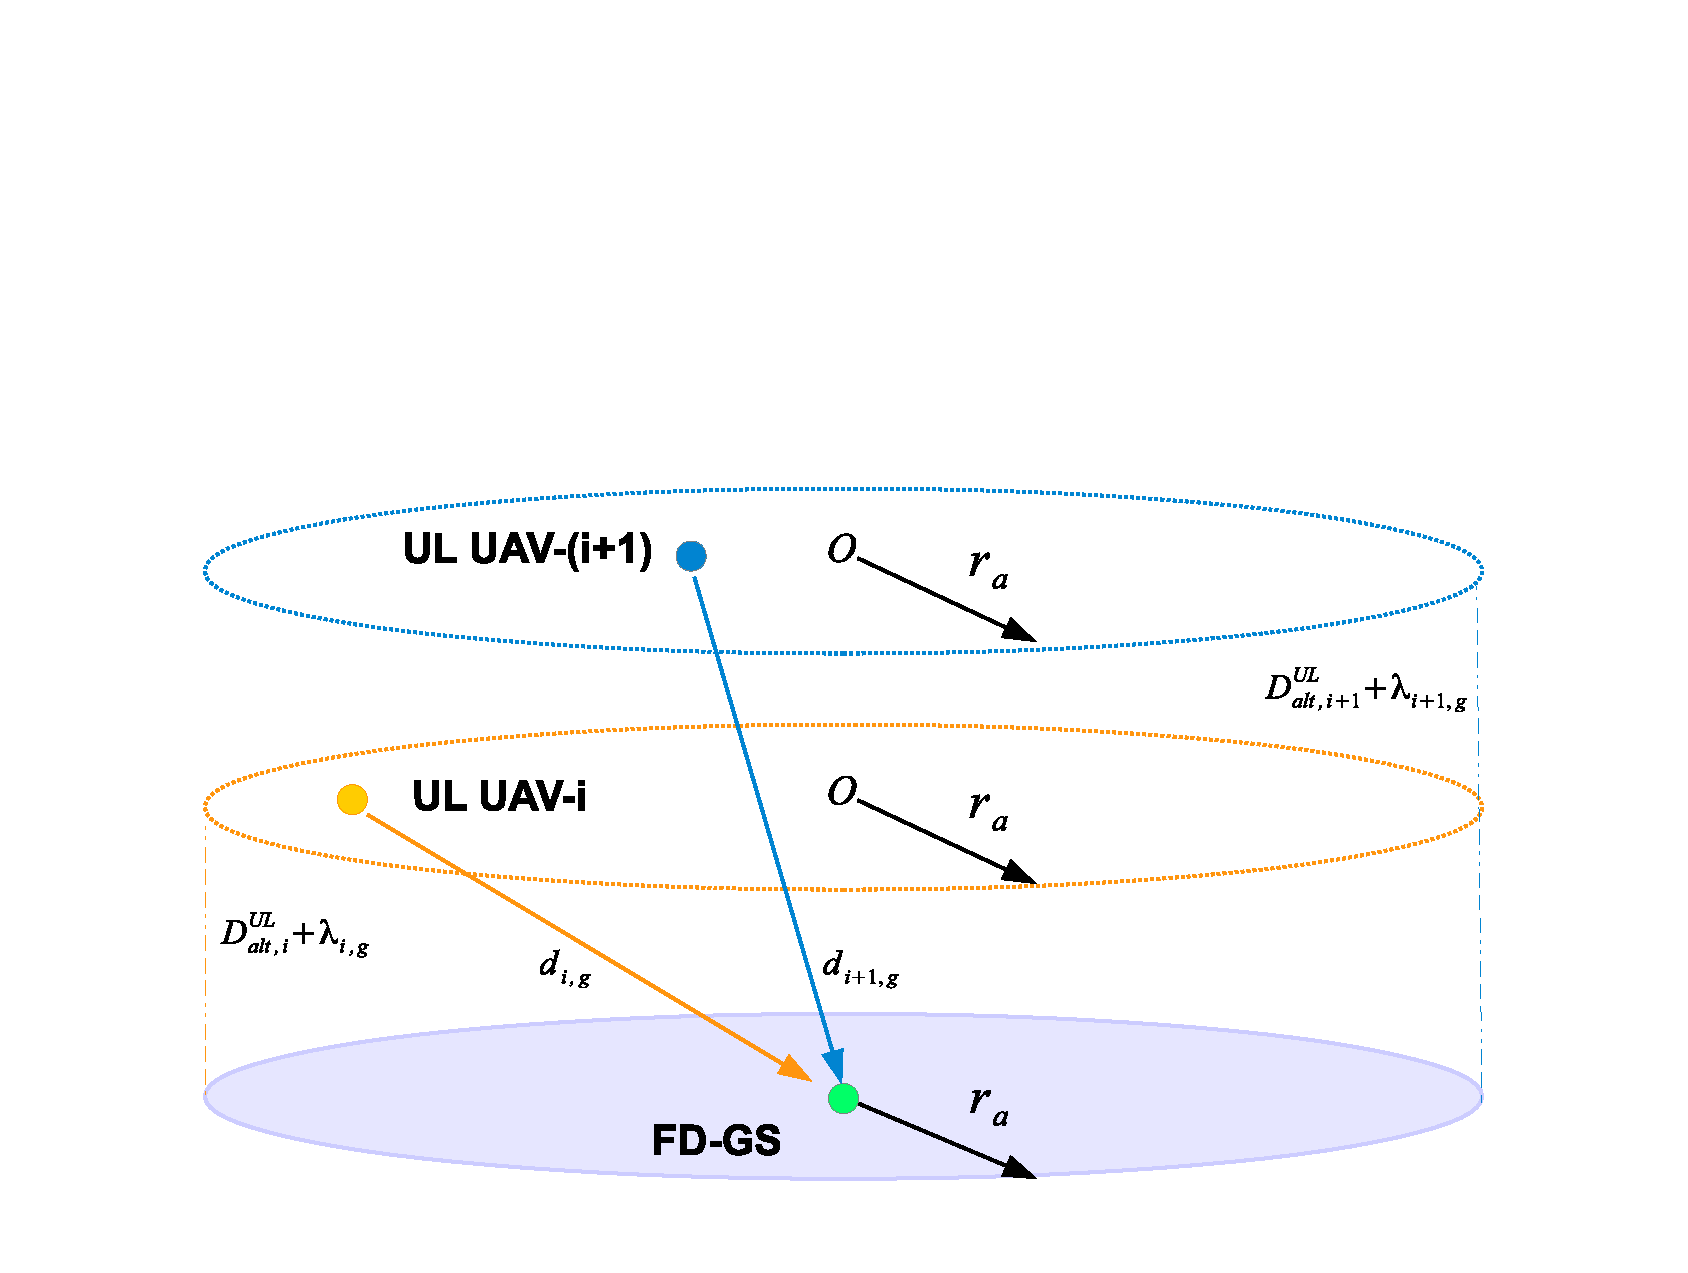
\includegraphics [width=0.6\columnwidth]{chap6_fig/UL_UAV_deployment.eps} 
%\vspace{-0.5cm}
\caption{An illustration of the UL UAV spatial locations. The spatial location of DL UAV-1 is described in the same fashion.}
\label{fig:HBD_multi_UAV_UL_UAV_deployment}
%\vspace{-0.5cm}
\end{figure}

Let the spatial location of the UAVs be uniformly distributed in a disc with radius $r_a$, angle $\left[0,2\pi\right)$, and origin $O$ above the FD-GS \cite{chetlur2017downlink}. By letting the FD-GS be located on the ground at origin $O$, we define the Euclidean distance (in km) between UL UAV-$i$ and the FD-GS as $d_{i,g}=\sqrt{D_{i,g}^2 + \big(D_{alt,i}^{UL} + \lambda_{i,g}\big)^2}$, where $D_{i,g}$ denotes the Euclidean distance between the projection of UL UAV-$i$ onto the ground plane and the FD-GS. Similarly, let the Euclidean distance between the FD-GS and DL UAV be $d_{g,1}=\sqrt{D_{g,1}^2+\big(D_{alt,1}^{DL} + \lambda_{g,1}\big)^2}$, where $D_{g,1}$ denotes the Euclidean distance between the projection of the DL UAV onto the ground plane and the FD-GS. The variable $\lambda_x$, $x \in \{(i,g),(g,1)\}$ denotes a minimum distance between the UAVs and the FD-GS such that $0 < \lambda_{x} < r_a$, $D_{alt,i}^{UL} \leq D_{alt,i+1}^{UL}$ and $\lambda_{i,g}<\lambda_{i+1,g}$, are satisfied to enable the SIC-based detection process at the FD-GS. Finally, we define the Euclidean distance between the UL and DL UAVs, i.e., inter-UAV distance, as $d_{i,1}$.

As the spatial locations of the UAVs follow a BPP, the PDF $f_{d_{x}}(w)$ of $d_{x}$ is defined as \cite[eq. (3)]{chetlur2017downlink} $f_{d_{x}}(w) =  \frac{2w}{r_a^2}$ where $x \in \{(i,g), (g,1)\}$, $D_{alt} + \lambda_{x} \leq w \leq \sqrt{ \big(D_{alt}+\lambda_{x}\big)^2+r_{a}^2}$, and $D_{alt} \in \{D_{alt,i}^{UL}, D_{alt,1}^{DL}\}$.

For the inter-UAV distance ($d_{i,1}$), the conditional PDF $f_{d_{i,1}}(w|d_{g,1})$ is given as \cite[eq. (2)]{chetlur2017downlink}:
%%%%%%%%%%%%%%%%%%%%%%%%%%%%%%%%%%%%%%%%%%%%%%%%%%%%%%%%%%%%%%%%%%%%%%%%%%%%%%%%%
\begin{eqnarray}
f_{d_{i,1}}(w|d_{g,1}) & = & \begin{cases}
		\hspace{0.25cm} \frac{2w}{r_a^2} \hspace{4.4cm}, \lambda_{i,1} \leq w \leq w_{m,1}\\
    \hspace{0.25cm} \frac{2w}{\pi r_a^2}\arccos\left( \frac{w^2 + d_{g,1}^2 - (r_a^2+\lambda_{i,1}^2)}{2d_{g,1}\sqrt{w^2 - \lambda_{i,1}^2}} \right), w_{m,1} < w \leq w_{p,1}\\ 
  \end{cases} \\\nonumber
\end{eqnarray}
%%%%%%%%%%%%%%%%%%%%%%%%%%%%%%%%%%%%%%%%%%%%%%%%%%%%%%%%%%%%%%%%%%%%%%%%%%%%%%%%%
where $w_{m,1}=\sqrt{(r_a - d_{g,1})^2 + (\lambda_{i,1})^2}$, $w_{p,1}=\sqrt{(r_a + d_{g,1})^2 + (\lambda_{i,1})^2}$, and $0 < \lambda_{i,1} <  w_{m,1}$ is the minimum distance between UL UAV-$i$ and the DL UAV. 

%Through the BPP model, a performance analysis of the HBD-UCS can be obtained with the spatial locations of the UAVs taken into consideration.

%\subsection{Received Signal at the Ground Station}

At the FD-GS, only residual SI is considered, with the SI channel modeled as a Rician fading channel to account for SI mitigation \cite{tan2018joint,ernest2019outage}. Let $x_{gs}$ and $x_i$ be the respective transmitted signals from the FD-GS and UL UAV-$i$. Then, the SOI and the SI signal at the FD-GS are $x_i$ and $x_{si}=x_{gs}$, respectively. Also, let $h_{i,g}$ denote the channel between UL UAV-$i$ and GS, and $h_{si}$ be the SI channel gain. The resultant received signal at GS can thus be written as \cite{sahai2013impact}:
%%%%%%%%%%%%%%%%%%%%%%%%%%%%%%%%%%%%%%%%%%%%%%%%%%%%%%%%%%%%%%%%%%%%%%%%%%%%%%%%%
\begin{eqnarray}
y_{gs} & = & \sum_{i=1}^{N_{UL}} \sqrt{\frac{P_i}{d_{i,g}^{n}}}h_{i,g}x_{i} + \sqrt{P_{si}} |\widetilde{h}_{si}|x_{si} + \sqrt{P_{si}}|h_{si}|\gamma_{\phi}w_{\phi} + {w_{g}}_,
\end{eqnarray} 
%%%%%%%%%%%%%%%%%%%%%%%%%%%%%%%%%%%%%%%%%%%%%%%%%%%%%%%%%%%%%%%%%%%%%%%%%%%%%%%%%
where $n$ is the pathloss exponent, $P_i$ is the transmit power of UL UAV-$i$, $P_{si}$ is the power of the SI, $\widetilde{h}_{si}$ is the error of the imperfect SI channel gain estimate, defined as $\widetilde{h}_{si}=h_{si}-\widehat{h}_{si}$, $\widehat{h}_{si}$ is the imperfect estimation of the SI channel gain, $w_{g}$ is the AWGN with zero-mean and variance $\sigma_g^2$, and $w_{\phi}$ is the Gaussian distributed phase noise with zero-mean and unit variance scaled by the strength of the phase noise $\gamma_{\phi}^2$ \cite{sahai2013impact}.\footnote{The phase noise term $\gamma_{\phi}$ reflects the jitter effect in oscillators due to hardware imperfections \cite{sahai2013impact}}

To model the worst case residual SI, the channel estimation error ($\widetilde{h}_{si}$) is modeled as a circularly symmetric zero-mean complex Gaussian random variable RV with variance $\epsilon$ \cite{tan2018joint,ernest2019outage}. Also, the total amount of SI suppression is $\frac{1}{\epsilon\sigma_g^2}$ \cite{ernest2019outage}. Finally, as $D_{alt,i}^{UL} \leq D_{alt,i+1}^{UL}$ and $\lambda_{i,g} < \lambda_{i+1,g}$, the SIC-based detection order begins from UL UAV-$i$ at the FD-GS, i.e., closest UL UAV, while treating the remaining $N_{UL}-i$ UL UAVs as interference.

%\subsection{Received Signal at the Downlink UAV}

At the DL UAV, the received signal can be written as:
%%%%%%%%%%%%%%%%%%%%%%%%%%%%%%%%%%%%%%%%%%%%%%%%%%%%%%%%%%%%%%%%%%%%%%%%%%%%%%%%%
\begin{eqnarray}
y_{DL} & = & \sqrt{\frac{P_g}{d_{g,i}^{n}}}h_{g,1}x_{gs} + \sum_{j=1}^{N_{UL}} \sqrt{\frac{P_j}{d_{j,1}^{n}}}h_{j,1}x_{j} + {w_{1}}_,
\end{eqnarray} 
%%%%%%%%%%%%%%%%%%%%%%%%%%%%%%%%%%%%%%%%%%%%%%%%%%%%%%%%%%%%%%%%%%%%%%%%%%%%%%%%%
where $P_g$ is the transmit power of the GS, $h_{g,1}$ is the channel between the FD-GS and the DL UAV, $h_{j,1}$ is the channel between UL UAV-$j$ and the DL UAV, and $w_{1}$ is the AWGN at the DL UAV with zero-mean and variance $\sigma_1^2$. As inter-UAV interference ($x_i$) is present at the DL UAV, we consider an imperfect SIC detector which removes inter-UAV interference first before detecting the SOI ($x_{gs}$). A summary of important notations is given in Table \ref{table:HBD_multi_UAV_summary_impt_notations}.

\begin{table}[]
\centering
\caption{Summary of Important Notations}
\label{table:HBD_multi_UAV_summary_impt_notations} 
\scalebox{0.8}{
\begin{tabular}{ll}
\hline
\textbf{Notations}		& \textbf{Description}																			\\  \hline \hline
$\Omega_X$						& Average received power																		\\
$\alpha_{i,j}, i\in\left\{g,1\right\}, j\in\left\{g,2\right\}, i \neq j$ & Strength of interference between $i$ and $j$				\\
$\epsilon$						& SI channel estimation error	at the FD-enabled GS					\\
$\gamma_{\phi}^2$			& Strength of phase noise at the FD- enabled GS oscillator	\\
$\sigma_g^2$					& Strength of AWGN at the FD-enabled GS											\\ 
$\sigma_2^2$					& Strength of AWGN at the UAV-2															\\ 
$r_a$ 								& Radius of the the disc 																		\\
$d_{i,1}$ 						& Euclidean distance between UL UAV-$i$ and the DL UAV 			\\
$d_{i,g}$ 						& Euclidean distance between UL UAV-$i$ and the FD-GS 			\\
$D_{alt,i}^{UL}$ 			& Altitude of UL UAV-$i$ 																		\\
$D_{alt,1}^{DL}$ 			& Altitude of the DL UAV 																		\\ 
$\lambda_x$, $x \in \{(i,g),(g,1)\}$ & Minimum distance between the UAVs and the FD-GS \\ \hline
\end{tabular}}
\end{table}
%A summary of important notations is also given in Table \ref{table:HBD_multi_UAV_summary_impt_notations}.

%%%%%%%%%%%%%%%%%%%%%%%%%%%%%%%%%%%%%%%%%%%%%%%%%%%%%%%%%%%%%%%%%%%%%%%%%%%%%%%%%%%%%%%%%%%%%%%%%%%%%%%%%%%%%%%%%%%%%%%%%%%%%%%%%%%%%%%%%
% Section 3 : Outage Probability Derivations
\section{Outage Probability} \label{HBD_multi_UAV_sec_outage}

In this section, outage probability expressions of the UL and DL UAVs are presented for the HBD-UCS. The outage probability expression for HD-UCS is also presented for benchmark comparison. Let $R^{j}_{i}$ and $R^{j}_{gs}$ for $j \in \{HBD, HD\}$ be the transmission rates of the UL UAV-$i$ and GS, respectively. For a fair comparison between the HBD-UCS and HD-UCS, we let $R_{i}^{HBD}=\frac{1}{2N_{UL}}R_{i}^{HD}$ and $R_{gs}^{HBD}=\frac{1}{2}R_{gs}^{HD}$ for uplink and downlink transmissions, respectively.

%, with sum rate defined as $R^{j}_{sum} = R^{j}_{i}+R^{j}_{gs}$

%%%%%%%%%%%%%%%%%%%%%%%%%%%%%%%%%%%%%%%%%%%%%%%%%%%%%%%%%%%%%%%%%%%%%%%%%%%%%%%%%%%%%%%%%%%%%%%%%%%%%%%%%%%%%%%%%%%%%%%%%%%%%%%%%%%%%%%%%
\subsection{Hybrid-Duplex Outage Probability}
For a SINR of $\frac{X_i d_i^{-n}}{1+\sum_{j=i+1}^{N}X_j d_j^{-n}}$ with $N$ interferers, where $X_i, 0 \leq i \leq N$ is a non-centered Chi-squared distributed random variable RV with Rician $K$ factor $K_i$, and $d_{l}^{-n}$ denotes the distance of transmitting node $l$, the outage probability is presented in the following Lemma.

\begin{lemma} \label{HBD_multi_UAV_lemma_P_out}
The outage probability $Pr\big(\mathcal{O}\big)$ for the outage event $\mathcal{O}$ at an arbitrary receiver is:
%%%%%%%%%%%%%%%%%%%%%%%%%%%%%%%%%%%%%%%%%%%%%%%%%%%%%%%%%%%%%%%%%%%%%%%%%%%%%%%%%
\begin{eqnarray} 
Pr\big(\mathcal{O}\big) & \approx & \sum_{q=0}^{K_{tr}} \sum_{l_1+\ldots+l_{N-q+1}=q+1} \alpha\big(q,\overline{P}_i,K_{i},\gamma\big) \binom{l_1 + \ldots + l_{N-q+1}}{l_1,\ldots, l_{N-q+1}} \nonumber \\
 & & \times \int_{-\infty}^{\infty} w_i^{n(q+1)}f_{d_i}(w_i) \Bigg( \prod_{j=1}^{N-i} E\Big\{X_{j}^{l_j}\Big\} \int_{-\infty}^{\infty} w_j^{-nl_j}f_{d_j}(w_j) dw_j \Bigg)  {dw_i}_,
\end{eqnarray}
%%%%%%%%%%%%%%%%%%%%%%%%%%%%%%%%%%%%%%%%%%%%%%%%%%%%%%%%%%%%%%%%%%%%%%%%%%%%%%%%%
\end{lemma}
where $\mathcal{O}=\Big\{ X_{i}, X_{j} : R \geq \log_{2}\Big(1 + \frac{X_i d_i^{-n}}{1+\sum_{j=i+1}^{N}X_j d_j^{-n}}\Big)\Big\}$, $R$ is the transmission rate, $K_{tr}$ is the truncation order, $\alpha\big(q,\overline{P}_i,K_i,\gamma\big) = (-1)^q \exp(-K_i) \frac{{L_q}^{(i)}(K_i)}{(1+q)!} \Big(\frac{(1+K_i)}{\overline{P}_i}\gamma\Big)^{q+1}$ is the CDF expansion of the RV $X_i$, $\overline{P}_i$ is the variance of $X_i$, $\gamma$ is the threshold, ${L_q}^{(0)}(\bullet)$ is the $q$-th degree, zero-order Laguerre polynomials \cite{tan2018joint, ernest2019outage}, and $E\{\bullet\}$ is the statistical expectation. Also, $E\Big\{X_{j}^{l_j}\Big\}=\Gamma(1+l_j) \left[\frac{\overline{P}_j}{1+K_{j}}\right]^{l_j} {}_1{F_1}(-l_j,1;-K_{j})$ is the $l_j^{th}$ moment of $X_j$ \cite[eq. (7)]{ernest2019outage} with ${}_1{F_1}(\bullet)$ representing the confluent Hypergeometric function \cite{ernest2019outage}.

\begin{proof}
The proof is provided in Appendix \ref{HBD_multi_UAV_lemma_P_out_proof}.
\end{proof} 

From Lemma \ref{HBD_multi_UAV_lemma_P_out}, the outage probability expressions of the UL and DL UAVs can be obtained.

\subsubsection{Uplink UAV-$i$}
Let $X_{i,g}=P_{i,g}|h_{i,g}|^2$ be the instantaneous received power of the SOI from UL UAV-$i$ at the FD-GS, where $P_{i,g}=\frac{P_i}{\sigma_g^2}$. Also, let $Y_{si,1}=P_{si}\gamma_{\phi}^2|h_{si}|^2$ and $Y_{si,2}=P_{si}\epsilon|\widetilde{h}_{si}|^2$ be the instantaneous received power of the residual SI components, where $P_{si}=P_{i,g}$. The symbols $X_{i,g}$ and $Y_{si,1}$ are non-centered Chi-squared distributed RVs with respective Rician $K$ factors $K_{i,g}$ and $K_{si,1}$ while $Y_{si,2}$ is an exponentially distributed RV. Defining the outage event of UL UAV-$i$ as $\mathcal{O}_{UL,i}^{HBD} = \Big\{ h_{i,g}, h_{si} : R_{i}^{HBD} \geq \log_{2}\Big(1 + \frac{X_{i,g}d_{i,g}^{-n}}{\sum_{j=i+1}^{N_{UL}} X_{j,g}d_{j,g}^{-n} + Y_{si,1} + Y_{si,2} + 1}\Big)\Big\}$, with threshold $\gamma_{gs}^{HBD} = 2^{R_{i}^{HBD}}-1$, the outage probability $Pr\big(\mathcal{O}_{UL,i}^{HBD}\big)$ of UL UAV-$i$ is presented in the following theorem:

\begin{theorem} \label{HBD_multi_UAV_theorem_P_out_UL_uav_i}
%%%%%%%%%%%%%%%%%%%%%%%%%%%%%%%%%%%%%%%%%%%%%%%%%%%%%%%%%%%%%%%%%%%%%%%%%%%%%%%%%
The outage probability at UL UAV-$i$ is
\begin{eqnarray} \label{HBD_multi_UAV_P_out_UL_uav_i}
Pr\big(\mathcal{O}_{UL,i}^{HBD}\big) & \approx & \sum_{q=0}^{K_{tr}} \sum_{l_1+\ldots+l_{N_{UL}-i+3}=q+1} \alpha\big(q,P_{i,g},K_{i,g},\gamma_{gs}^{HBD}\big) \Delta\big(D_{alt,i}^{UL},\lambda_{i,g},q\big) \nonumber\\ 
& & \hspace{-1cm} \times \binom{l_1 + \ldots + l_{N_{UL}-i+3}}{l_1,\ldots, l_{N_{UL}-i+3}} E\Big\{Y_{si,1}^{l_1}\Big\} E\Big\{Y_{si,2}^{l_2}\Big\} \prod_{j=1}^{N_{UL}-i} E\Big\{X_{j,g}^{l_j}\Big\} \overline{\Delta}\big(D_{alt,j}^{UL},\lambda_{j,g},l_j\big)_,
\end{eqnarray}
%%%%%%%%%%%%%%%%%%%%%%%%%%%%%%%%%%%%%%%%%%%%%%%%%%%%%%%%%%%%%%%%%%%%%%%%%%%%%%%%%
where $n \neq 2$, $\Delta\big(D_{alt,i}^{UL},\lambda_{i,g},q\big) = \frac{2}{[n(q+1)+2]r_a^2} \Big( \big[\big(D_{alt,i}^{UL} + \lambda_{i,g}\big)^2 + r_a^2 \big]^{\frac{n(q+1)+2}{2}} - \big[\big(D_{alt,i}^{UL} + \lambda_{i,g}\big)^2 \big]^{\frac{n(q+1)+2}{2}} \Big)$, and $\overline{\Delta}\big(D_{alt,j}^{UL},\lambda_{j,g},l_j\big) = \frac{2}{[2-nl_j]r_a^2} \Big( \big[\big(D_{alt,j}^{UL} + \lambda_{j,g}\big)^2 + r_a^2 \big]^{\frac{2-nl_j}{2}} - \big[\big(D_{alt,j}^{UL} + \lambda_{j,g}\big)^2  \big]^{\frac{2-nl_j}{2}} \Big)$.
\end{theorem}
\begin{proof}
Applying Lemma \ref{HBD_multi_UAV_lemma_P_out} and integrating the resulting expression over the PDFs $f_{d_{i,g}}(w_i)$ and $f_{d_{j,g}}(w_j)$ yields Theorem \ref{HBD_multi_UAV_theorem_P_out_UL_uav_i}.
\end{proof}

As $2-nl_j$ is present in the denominator of $\overline{\Delta}\big(D_{alt,j}^{UL},\lambda_{j,g},l_j\big)$, Theorem \ref{HBD_multi_UAV_theorem_P_out_UL_uav_i} is valid only when $n \neq 2$. However, it must be noted that selecting $n \approx 2$, e.g., $n = 2 + 10^{-6}$, enables Theorem \ref{HBD_multi_UAV_theorem_P_out_UL_uav_i} to be applied for outage probability analysis involving free space path loss scenarios.\footnote{Selecting $n \approx 2$, e.g., $n = 2 + 10^{-6}$, allows $\overline{\Delta}\big(D_{alt,j}^{UL},\lambda_{j,g},l_j\big)$ to be evaluated for free space path loss scenarios while avoiding a zero in the denominator.} \textcolor{black}{\footnote{\textcolor{black}{To analytically ascertain the accuracy of the new power series expressions in this chapter, one will need to conduct a truncation analysis. Work in this direction is left as an open research challenge which can be addressed in future studies.}}}

\subsubsection{Downlink UAV}

At the DL UAV, let $X_{g,1}=P_{g,1}|h_{g,1}|^2$ be the instantaneous received power of the SOI from the GS at the DL UAV, where $P_{g,1}=\frac{P_g}{\sigma_1^2}$. Also, let $X_{j,1}=P_{j,1}\beta_{j,1}|h_{j,1}|^2$ be the instantaneous received powers of the inter-UAV interference from UL UAV-$j$ due to HBD transmissions, where $P_{j,1}=\frac{P_j}{\sigma_1^2}$, and $0 \leq \beta_{j,1} \leq 1$ denotes the strength of the residual interference due to imperfect SIC. The symbols $X_{g,1}$ and $X_{j,1}$ are non-centered Chi-squared distributed RVs with respective Rician $K$ factors $K_{g,1}$ and $K_{j,1}$. Defining the outage event at the DL UAV as $\mathcal{O}_{DL}^{HBD} = \Big\{ h_{g,1}, h_{j,1} : R_{gs}^{HBD} \geq \log_{2}\Big(1 + \frac{X_{g,1}d_{g,1}^{-n}}{\sum_{j=1}^{N_{UL}}X_{j,1}d_{j,1}^{-n} + 1}\Big)\Big\}$, the outage probability expression for the DL UAV is presented in the following theorem.

\begin{theorem} \label{HBD_multi_UAV_theorem_P_out_DL_uav}
%%%%%%%%%%%%%%%%%%%%%%%%%%%%%%%%%%%%%%%%%%%%%%%%%%%%%%%%%%%%%%%%%%%%%%%%%%%%%%%%%
The HBD outage probability at the DL UAV is
\begin{eqnarray} \label{HBD_multi_UAV_P_out_DL_uav}
Pr\big(\mathcal{O}_{DL}^{HBD}\big) & \approx & \sum_{q=0}^{K_{tr}} \sum_{l_1+\ldots+l_{N_{UL}+1}=q+1} \alpha\big(q,P_{g,1},K_{g,1},\gamma_{DL}^{HBD}\big) \binom{l_1 + \ldots + l_{N_{UL}-i+3}}{l_1,\ldots, l_{N_{UL}-i+3}} \nonumber\\ 
 & & \hspace{0.5cm} \times \int_{L_1}^{L_2} \frac{2w_{g,1}^{n(q+1)+1}}{r_a^2} \Bigg( \prod_{j=1}^{N_{UL}} E\Big\{X_{j,1}^{l_j}\Big\} \Xi_{j,1}(w_{g,1},l_j) \Bigg){dw_{g,1}}_,
\end{eqnarray}
%%%%%%%%%%%%%%%%%%%%%%%%%%%%%%%%%%%%%%%%%%%%%%%%%%%%%%%%%%%%%%%%%%%%%%%%%%%%%%%%%
where $L_1 = D_{alt,1}^{DL} + \lambda_{g,1}$, $L_2 = \sqrt{\big(D_{alt,1}^{DL} + \lambda_{g,1}\big)^2 + r_{a}^2}$, $\gamma_{DL}^{HBD} = 2^{R_{gs}^{HBD}}-1$, and $\Xi_{j,1}(w_{g,1},l_j) = \frac{2\big[(w_{m,1})^{2-nl_j} - \lambda_{j,1}^{2-nl_j}\big]}{r_a^2[2-nl_j]} + \int_{w_{m,1}}^{w_{p,1}} \frac{2w_{j,1}}{\pi r_a^2}\arccos\Bigg( \frac{w_{j,1}^2 + w_{g,1}^2 - (r_a^2+\lambda_{j,1}^2)}{2w_{g,1}\sqrt{w_{j,1}^2 - \lambda_{j,1}^2}} \Bigg) {dw_{j,1}}$.
%%%%%%%%%%%%%%%%%%%%%%%%%%%%%%%%%%%%%%%%%%%%%%%%%%%%%%%%%%%%%%%%%%%%%%%%%%%%%%%%%%
%\begin{eqnarray}
%\Xi_{j,1}(w_{g,1},l_j) & = & \frac{2\big[(w_{m,1})^{2-nl_j} - \lambda_{j,1}^{2-nl_j}\big]}{r_a^2[2-nl_j]} \nonumber \\
 %& & \hspace{-2.7cm} + \int_{w_{m,1}}^{w_{p,1}} \frac{2w_{j,1}}{\pi r_a^2}\arccos\Bigg( \frac{w_{j,1}^2 + w_{g,1}^2 - (r_a^2+\lambda_{j,1}^2)}{2w_{g,1}\sqrt{w_{j,1}^2 - \lambda_{j,1}^2}} \Bigg) {dw_{j,1}}_.
%\end{eqnarray}
%%%%%%%%%%%%%%%%%%%%%%%%%%%%%%%%%%%%%%%%%%%%%%%%%%%%%%%%%%%%%%%%%%%%%%%%%%%%%%%%%%
\end{theorem}
\begin{proof}
Theorem \ref{HBD_multi_UAV_theorem_P_out_DL_uav} is proven using the same approach in Theorem \ref{HBD_multi_UAV_theorem_P_out_UL_uav_i}.
\end{proof}

%With (\ref{P_out_UL_uav_i}) and (\ref{P_out_DL_uav}), a stochastic geometry-based outage probability analysis of the HBD-UCS over Rician fading UAV channels is now possible. 

%%%%%%%%%%%%%%%%%%%%%%%%%%%%%%%%%%%%%%%%%%%%%%%%%%%%%%%%%%%%%%%%%%%%%%%%%%%%%%%%%%%%%%%%%%%%%%%%%%%%%%%%%%%%%%%%%%%%%%%%%%%%%%%%%%%%%%%%%
\subsection{Half-Duplex Outage Probability}
We compare the HBD-UCS with HD-UCS as a benchmark scheme. For the HD-UCS, an outage is declared for UL UAV-$i$ when $R_{i}^{HD} \geq \log_{2}\big(1 + X_{i,g}d_{i,g}^{-n}\big)$. Similarly, an outage is declared for the DL UAV when $R_{gs}^{HD} \geq \log_{2}\big(1 + X_{g,1}d_{g,1}^{-n}\big)$. Thus, the HD-UCS outage events for UL UAV-$i$ and the DL UAV are defined as $\mathcal{O}_{UL,i}^{HD} = \big\{ h_{i,g} : R_{i}^{HD} \geq \log_{2}\big(1 + X_{i,g}d_{i,g}^{-n}\big)\big\}$ and $\mathcal{O}_{DL}^{HD} = \Big\{ h_{g,1} : R_{gs}^{HD} \geq \log_{2}\Big(1 + X_{g,1}d_{g,1}^{-n}\Big)\Big\}$, respectively. Following the same approach presented in Appendix \ref{HBD_multi_UAV_lemma_P_out_proof}, the HD-UCS outage probability expressions for UL UAV-$i$ and the DL UAV are:
%%%%%%%%%%%%%%%%%%%%%%%%%%%%%%%%%%%%%%%%%%%%%%%%%%%%%%%%%%%%%%%%%%%%%%%%%%%%%%%%%%
\begin{eqnarray}
 Pr\big(\mathcal{O}_{UL,i}^{HD}) & \hspace{-0.1cm} \approx & \hspace{-0.1cm} \sum_{q=0}^{K_{tr}} \alpha\big(q,P_{i,g},K_{i,g},\gamma_{gs}^{HD}\big) \Delta\big(D_{alt,i}^{UL},\lambda_{i,g},q\big)_, \\
 Pr\big(\mathcal{O}_{DL}^{HD}) & \hspace{-0.1cm} \approx & \hspace{-0.1cm} \sum_{q=0}^{K_{tr}} \alpha\big(q,P_{g,1},K_{g,1},\gamma_{DL}^{HD}\big) \Delta\big(D_{alt,1}^{DL},\lambda_{g,1},q\big)_,
\end{eqnarray}
%%%%%%%%%%%%%%%%%%%%%%%%%%%%%%%%%%%%%%%%%%%%%%%%%%%%%%%%%%%%%%%%%%%%%%%%%%%%%%%%%%
where $\gamma_{gs}^{HD} = 2^{R_{1}^{HD}}-1$ and $\gamma_{DL}^{HD} = 2^{R_{gs}^{HD}}-1$.

%%%%%%%%%%%%%%%%%%%%%%%%%%%%%%%%%%%%%%%%%%%%%%%%%%%%%%%%%%%%%%%%%%%%%%%%%%%%%%%%%%%%%%%%%%%%%%%%%%%%%%%%%%%%%%%%%%%%%%%%%%%%%%%%%%%%%%%%%
% Section 4: Numerical Results
\section{Numerical Results} \label{HBD_multi_UAV_sec_num_res}

The outage probability of the HBD-UCS is analyzed in this section for Rician $K$ factors of 10 dB \cite[Table V]{matolak2017air_suburban}, $0\text{ dB} \leq P_t \leq 30\text{ dB}$, $P_{i,g} = P_{g,1} = P_{j,1} = P_t$, $\sigma_g^2 = \sigma_{1}^2 = -131\text{dBm}$ \cite{itu2011m2233}, $R_{x}^{HD} =  0.1 \text{b/s/Hz}, i \in \{i,gs\}$, $\gamma_{\phi}^2 = -140\text{dBm}$, $\epsilon=0.01$ \cite{ernest2019outage}, $r_a=4$ km, $n \approx 2$ \cite[Table III]{matolak2017air_suburban}, $N_{UL}=3$, $\lambda_{1,g} =1.3$, $\lambda_{2,g} =1.4$, $\lambda_{3,g} =1.5$, $\beta_{j,1}=0.5^2$, and Monte Carlo simulations using $10^{5}$ samples.

\begin{figure*}[h]
\centering
%\vspace{-0.5cm}
\subfloat[Uplink outage probability.]{\includegraphics [width=0.45\columnwidth]{chap6_fig/hbd_UL_outage.eps}
\label{fig:HBD_multi_UAV_pout_UL}}
\hfil
\subfloat[Downlink outage probability for $\lambda_{1,1} = 1.4$, $\lambda_{2,1} = 1.3$, and $\lambda_{3,1} = 1.2$.]{\includegraphics [width=0.45\columnwidth]{chap6_fig/hbd_DL_outage.eps}
\label{fig:HBD_multi_UAV_pout_DL}}
\hfil
\subfloat[Impact of SI cancellation and phase noise on uplink outage probability.]{\includegraphics [width=0.45\columnwidth]{chap6_fig/hbd_UL_outage_SI_cancellation.eps}
\label{fig:HBD_multi_UAV_pout_SI_cancellation}}
\caption{Outage probability of the HBD-UCS.}
\label{fig:HBD_multi_UAV_pout}
%\vspace{-0.51cm}
\end{figure*}

%%%%%%%%%%%%%%%%%%%%%%%%%%%%%%%%%%%%%%%%%%%%%%%%%%%%%%%%%%%%%%%%%%%%%%%%%%%%%%%%%%
% At low $P_t$ regimes, the HBD-UCS outperforms the HD-UCS in terms of uplink and downlink outage probability. 
% Additionally, for uplink transmissions, recall that the FD-GS detects UL UAV-$i$ by treating the remaining $N_{UL}-i$ UL UAVs as interference. As such, UL UAV-1 is seen to exhibit higher outage probability then UL UAV-2 and UAV-3, with similar observations also noted for the subsequent UL UAVs.
% It is also seen that, depending on the number of interfering UL UAVs, the HBD-UCS can also attain lower downlink outage probability than the HD-UCS at moderate $P_t$ regimes, e.g., $N_{UL}\in \{2,3\}$.
% At high $P_t$ regimes, the HD-UCS attains lower outage probability than the HBD-UCS for both uplink and downlink outage probability. 
% For uplink transmissions, error floors are observed since the detection process at the FD-GS becomes interference-limited due to interference from the remaining $N_{UL}-i$ UL UAVs. Similarly, for downlink transmissions, error floors are observed due to the downlink UAV becoming interference-limited as a result of residual SIC interference. 
% Thus, it is shown that the HBD-UCS is well suited for multi-UAV networks since UAV communications operate at low $P_t$ regimes. \footnote{It is worth noting that UAVs largely operate at low $P_t$ regimes due to SWAP restrictions. For instance, $29\text{dBm} \leq P_t \leq 40\text{dBm}$ was noted in \cite{ITU2011}, while in \cite{zeng2018cellularconnecteduav}, cellular-to-UAV links were evaluated for $P_t = 20\text{dBm}$. The values found in \cite{ITU2011,zeng2018cellularconnecteduav} translates into $-10 \text{dB} \leq P_t \leq 10 \text{dB}$.}
%%%%%%%%%%%%%%%%%%%%%%%%%%%%%%%%%%%%%%%%%%%%%%%%%%%%%%%%%%%%%%%%%%%%%%%%%%%%%%%%%%

\begin{observation}
\emph{\emph{With effective SI mitigation, the HBD-UCS achieves lower outage probability at low $P_t$ regimes than the HD-UCS and is able to fulfill $PER$ requirements for CNPC links in LTE networks.}}
\end{observation}

The outage probability of the HBD-UCS is compared against the HD-UCS for both UL and DL transmissions in Fig. \ref{fig:HBD_multi_UAV_pout}. At low $P_t$ regimes, the HBD-UCS outperforms the HD-UCS in terms of UL and DL outage probability. In particular, the HBD-UCS is able to fulfill $PER$ requirements for UAV control links over Long Term Evolution (LTE) networks, i.e., $PER<10^{-3}$ \cite{tr362017}.\footnote{Outage probability can be used to represent $PER$ if the transmitted signals span over one fading block \cite{ernest2019outage}.} Additionally, for UL transmissions, recall that the FD-GS detects UL UAV-$i$ by treating the remaining $N_{UL}-i$ UL UAVs as interference. As such, UL UAV-1 is seen to exhibit higher outage probability than UL UAV-2 and UAV-3, with similar observations also noted for the subsequent UL UAVs. It is also seen that, depending on the number of interfering UL UAVs, the DL UAV can also attain lower DL outage probability than the HD-UCS at moderate $P_t$ regimes, e.g., $N_{UL}\in \{2,3\}$. 

At high $P_t$ regimes, the HD-UCS attains lower outage probability than the HBD-UCS for both UL and DL outage probability. For UL transmissions, error floors are observed since the detection process at the FD-GS becomes interference-limited due to interference from the remaining $N_{UL}-i$ UL UAVs. Similarly, for DL transmissions, error floors are observed due to the DL UAV becoming interference-limited as a result of residual SIC interference.  Thus, it is shown that the HBD-UCS is well suited for multi-UAV networks since UAV communications operate at low $P_t$ regimes.\footnote{It is worth noting that UAVs largely operate at low $P_t$ regimes due to size, weight, and power restrictions. For instance, $29\text{dBm} \leq P_t \leq 40\text{dBm}$ was noted in \cite{itu2011m2233}, while in \cite{zeng2018cellularconnecteduav}, cellular-to-UAV links were evaluated for $P_t = 20\text{dBm}$. The values found in \cite{itu2011m2233,zeng2018cellularconnecteduav} translates into $-10 \text{dB} \leq P_t \leq 10 \text{dB}$.}\footnote{Outage probability can be further reduced when the transmit power and trajectory of the UAVs are optimized iteratively. For transmit power optimization, one should consider the spatial location of the UAVs and the trajectory. For trajectory optimization, both the spiral and oval trajectory processes should be considered to maintain a uniform distribution under the BPP model \cite{enayati2019moving}.} The impact of SI cancellation and phase noise on uplink outage probability is seen in Fig. \ref{fig:HBD_multi_UAV_pout_SI_cancellation}. It is observed that an increase in either $\gamma_{\phi}^2$ or $\epsilon$ causes the outage probability of the UL UAVs to increase. Furthermore, an increasing $\gamma_{\phi}^2$ causes higher outage probability than an increasing $\epsilon$ due to higher residual SI at the FD-GS. Thus, the reliability of UL UAV transmissions in an HBD-UCS hinges on having effective SI mitigation architectures with low phase noise FD transceivers at the GS. 

\begin{figure}[]
\centering
\subfloat[Uplink outage probability.]{\includegraphics [width=0.45\columnwidth]{chap6_fig/hbd_UL_outage_height.eps}
\label{fig:HBD_multi_UAV_hbd_UL_outage_height}} 
\hfil
\subfloat[Downlink outage probability.]{\includegraphics [width=0.45\columnwidth]{chap6_fig/hbd_DL_outage_height.eps}
\label{fig:HBD_multi_UAV_hbd_DL_outage_height}}
\caption{Impact of height and minimum distance on the outage probability of the HBD-UCS at $P_t = 5$ dB, $\beta = 1$, $\lambda_{g,1} = 0.1$, and $D_{alt}^{UL}=D_{alt,i}^{UL}$.}
\label{fig:HBD_multi_UAV_pout_height}
%\vspace{-0.6cm}
\end{figure}

%%%%%%%%%%%%%%%%%%%%%%%%%%%%%%%%%%%%%%%%%%%%%%%%%%%%%%%%%%%%%%%%%%%%%%%%%%%%%%%%%%
% In Fig. \ref{fig:pout_height}, the impact of height and minimum distance on the outage probability of the HBD-UCS is analyzed.
% For UL transmissions, a lower outage probability is attained when $ 0 \leq D_{alt}^{UL} \leq 1$ and $\lambda_{i,g}$ is reduced, since weaker UL interference is experienced. However, when $D_{alt}^{UL} > 1$, outage probability increases due to a weaker SOI. Similarly, increasing $\lambda_{i,g}$ leads to higher outage probability as the SOI is further weakened. 
% For DL transmissions, increasing $D_{alt,1}^{DL}$ leads to higher outage probability for the HBD-UCS and HD-UCS due to a weaker SOI. It is also observed that increasing $\lambda_{i,1}$ reduces outage probability since inter-UAV interference is weakened. 
% Therefore, as seen in Fig. \ref{fig:pout_height}, one may have to consider other approaches if support for UAVs deployed at high altitudes is required. Nonetheless, Fig. \ref{fig:pout} and Fig. \ref{fig:pout_height} have demonstrated that the multi-UAV network with HBD-UCS is able to support more UAVs concurrently on the same spectrum while attaining a lower outage probability than the HD-UCS.
%%%%%%%%%%%%%%%%%%%%%%%%%%%%%%%%%%%%%%%%%%%%%%%%%%%%%%%%%%%%%%%%%%%%%%%%%%%%%%%%%%

\begin{observation}
\emph{\emph{Increasing the altitude of the UAVs leads to higher outage probability for the HBD-UCS.}}
\end{observation}

In Fig. \ref{fig:HBD_multi_UAV_pout_height}, the impact of height and minimum distance on the outage probability of the HBD-UCS is analyzed. For UL transmissions, a lower outage probability is attained when $ 0 \leq D_{alt}^{UL} \leq 1$ and \textcolor{black}{when} $\lambda_{i,g}$ is reduced, since weaker UL interference is experienced. However, when $D_{alt}^{UL} > 1$, outage probability increases due to a weaker SOI. Similarly, increasing $\lambda_{i,g}$ leads to higher outage probability as the SOI is further weakened. For DL transmissions, increasing $D_{alt,1}^{DL}$ leads to higher outage probability for the HBD-UCS and HD-UCS due to a weaker SOI. It is also observed that increasing $\lambda_{i,1}$ reduces outage probability since inter-UAV interference is weakened. Therefore, as seen in Fig. \ref{fig:HBD_multi_UAV_pout_height}, one may have to consider other approaches if support for UAVs deployed at high altitudes is required. Nonetheless, Fig. \ref{fig:HBD_multi_UAV_pout} and Fig. \ref{fig:HBD_multi_UAV_pout_height} have demonstrated that the multi-UAV network with HBD-UCS is able to support more UAVs concurrently on the same spectrum while attaining a lower outage probability than the HD-UCS.

%%%%%%%%%%%%%%%%%%%%%%%%%%%%%%%%%%%%%%%%%%%%%%%%%%%%%%%%%%%%%%%%%%%%%%%%%%%%%%%%%%%%%%%%%%%%%%%%%%%%%%%%%%%%%%%%%%%%%%%%%%%%%%%%%%%%%%%%%
% Section 5: Conclusion
\section{Chapter Summary} \label{HBD_multi_UAV_sec_conclusion}

In this chapter, the outage probability analysis of a multi-UAV network with HBD-UCS is investigated within a stochastic geometry framework. It is demonstrated that at low transmit power regimes, the HBD-UCS achieves lower outage probability than the HD-UCS for both uplink and downlink transmissions. It is also shown that the HBD-UCS can support uplink and downlink transmissions that are more reliable than the HD-UCS, when the UAV operating altitude is increased. Thus, we demonstrate that the HBD-UCS is able to concurrently support more UAVs while achieving a higher reliability than the HD-UCS.

To enable a greater number of deployed UAVs in multi-UAV networks with ease of deployment, one can consider tapping on existing cellular infrastructure to support multi-UAV communications. In this spirit, NOMA-aided multi-UAV communications is examined in the next chapter for FD heterogeneous networks. 




\counterwithin*{observation}{subsection}
\renewcommand{\theobservation}{\thesubsection.\arabic{observation}}



%---------------------------------------------------------------------------------
\chapter{NOMA-Aided Multi-UAV Communications in Full-Duplex Heterogeneous Networks}
\label{chap:NOMA_aided_multi_UAV_FD_HetNet}
%---------------------------------------------------------------------------------

\section{Introduction}

Apart from FD-based HBD-UCSs, one can also consider power-domain NOMA as a means to further improve spectrum efficiency in UAV communications. The concept of NOMA hinges on the fact that nodes in NOMA-aided systems are multiplexed in the power-domain to share the same spectrum. In contrast, conventional orthogonal multiple access schemes employ orthogonal allocation of time-frequency resource blocks for each node in the network. Thus, compared to orthogonal multiple access systems, NOMA-aided systems are capable of achieving higher spectrum utilization. When adopted for multi-UAV communications, superposition coding is employed to enforce unequal power allocation for all UAVs and GSs. Thereafter, the desired messages are recovered at the receivers via SIC when the interference is stronger than the desired message \cite{liu2019uav,yang2016general,cui2016novel,kader2018full,salehi2019meta,weber2007transmission,islam2017power}. For receivers experiencing weak interference, the desired message is simply detected by treating interference as noise \cite{liu2019uav,islam2017power}.\footnote{The work in this chapter is derived from \cite{ernest2019hetnet}, which has been submitted for publication.}

Already, NOMA has been investigated as a means to improve spectrum efficiency in heterogeneous networks (HetNets) for cellular communications \cite{moltafet2018optimal,liu2018heterogeneous} and UAV communications \cite{liu2019dsf}. Although promising, the orthogonal allocation of time-frequency resources is still necessary as power-domain multiplexing is only employed during UL or DL transmissions \cite{ernest2019noma,ding2018coexistence}. 

To further address spectrum scarcity, one can consider integrating NOMA-aided multi-UAV communications into FD HetNets, i.e., FD-HetNets, comprising FD-capable GSs (FD-GSs) and HD macro base stations (MBSs). In particular, implementing NOMA-aided multi-UAV communications in FD-HetNets enable UL UAVs and DL UAVs, equipped with conventional HD transceivers, to simultaneously operate on the same spectrum thanks to the operation of FD-GSs. As compared to conventional NOMA-aided HD-HetNets, where all nodes operate in HD mode, higher spectrum efficiency can be attained via NOMA-aided FD-HetNets. However, such FD-based systems are also impaired by residual SI due to carrier phase noise and imperfect SI channel estimation \cite{sahai2013impact}, and interference from UL UAVs \cite{tan2018joint,ernest2019noma,ernest2019power}.

\subsection{Related Literature}
Despite being limited by residual SI and UL interference, NOMA-aided FD-HetNets have started receiving interest in the literature as a potential solution to address spectrum scarcity. For instance, a power control technique was proposed in \cite{lei2018noma} for interference management in a NOMA-aided FD-HetNet, with similar works on NOMA-aided HD-HetNets \cite{moltafet2018optimal,liu2018heterogeneous} noted. For UAV communications in FD-HetNets and HD-HetNets, there exists limited studies in the literature. To illustrate, resource allocation and UAV placement in HD-HetNets were investigated in \cite{liu2019dsf} and \cite{sharma2016uavs}, respectively, while \cite{zhang20183} and \cite{zhang2018number} analyzed the placement of aerial BSs for FD-HetNets. From the above studies, an analysis of NOMA-aided multi-UAV communications in FD-HetNets is, to the best of our knowledge, unavailable in the literature. Although there exists some works on NOMA-aided FD-HetNets and NOMA-aided HD-HetNets in cellular networks, the conclusions from those studies may not be readily applied for multi-UAV communications due to differences in operating environments and deployment constraints between cellular and multi-UAV systems.

One such difference is the channel model for both cellular and UAV communications. In cellular communications, Rayleigh fading \cite{ding2018coexistence} and Nakagami-$m$ fading \cite{chu2018performance,hou2018multiple} are commonly assumed. However, apart from UAV communications taking place over Rayleigh fading \cite{zhao2019joint,mei2019uplink} and Nakagami-$m$ fading \cite{chetlur2017downlink}, other types of fading can also be encountered. For instance, transmissions over Rician fading channels have been noted for UAV-to-GS links \cite{matolak2017air_suburban,matolak2017air_water,sun2017air_hilly,tan2018joint,ernest2019noma,ernest2019power,nasir2019uav,nguyen2018novel} and UAV-to-UAV links \cite{tan2018joint,ernest2019power,yuan2018capacity}.

Another difference stems from the spatial distribution of nodes in cellular and UAV communications. As discussed earlier, the application of UAVs in future wireless networks has garnered intense interest in deploying UAV-aided wireless connectivity via aerial BSs or relays. \textcolor{black}{Hence, the spatial location and mobility of the UAVs  need to be accounted for before any accurate performance evaluation}. To accomplish such a feat, one can employ the useful tools of stochastic geometry for multi-UAV networks. A common technique seen in the literature involves modeling the spatial location of UEs as a PPP. However, it has since been shown in \cite{chetlur2017downlink} that the PPP model is unsuitable for multi-UAV networks, as the number of deployed UAVs is usually fixed. Such an instance can be illustrated when UAVs function as aerial BSs in a given region \cite{chetlur2017downlink,wang2018modeling}. In such scenarios, the homogeneous BPP can be used to provide an accurate modeling of the UAV spatial locations \cite{chetlur2017downlink,wang2018modeling}. In spite of several studies that have analyzed multi-UAV networks using the BPP model, e.g., \cite{chetlur2017downlink,wang2018modeling,enayati2019moving}, similar studies involving NOMA-aided multi-UAV communications in FD-HetNets are lacking in the literature.

Based on the above discussions, an ergodic capacity analysis of NOMA-aided multi-UAV communications in a FD-HetNet is conducted in this chapter. By considering Rician fading channels and the BPP model for UAV spatial location modeling, we demonstrate the feasibility and advantages of NOMA-aided multi-UAV communications in FD-HetNets in a realistic setting. 

%%%%%%%%%%%%%%%%%%%%%%%%%%%%%%%%%%%%%%%%%%%%%%%%%%%%%%%%%%%%%%%%%%%%%%%%%%%%%%%%%%%%%%%%%%%%%%%%%%%%%%%%%%%%%%%%%%%%%%%%%%%%%%%%%%%%%%%%%
% Section 2 : System Model
\section{System Model} \label{NOMA_aided_multi_UAV_FD_HetNet_sec_sys_model}
\begin{figure} [tpb]
\centering
\vspace{-0.7cm}
\includegraphics [width=0.6\columnwidth]{chap7_fig/block_diagram3.eps} 
\vspace{-2cm}
\caption{The FD-HetNet for NOMA-aided multi-UAV communications is illustrated here. The FD-GS in the FD-HetNet enables HD uplink and downlink UAVs and the HD MBS to concurrently share the same spectrum for NOMA transmissions. Through the BPP, it is assumed that the spatial locations of the deployed UAVs and the MBS follow a uniform distribution around a disc, with origin $O$ at the FD-GS and radius $r_a$.}
\label{fig:NOMA_aided_multi_UAV_FD_HetNet_block_diagram}
%\vspace{-0.3in}
\end{figure}

Consider a FD-HetNet supporting NOMA-aided multi-UAV communications in a suburban environment (Fig. \ref{fig:NOMA_aided_multi_UAV_FD_HetNet_block_diagram}). The FD-HetNet comprises $N_{U}$ HD single-antenna UL UAVs, $N_D$ HD single-antenna DL UAVs, one HD single-antenna MBS, and a FD-GS. The FD-GS is assumed to be operating with one antenna each for signal transmission and reception. It is also assumed that the FD-GS receives uplink data from the $N_{U}$ UL UAVs and MBS-to-GS data from the MBS while concurrently transmitting DL data to the $N_D$ DL UAVs on the same spectrum through power-domain NOMA.\footnote{It is worth noting that such a system model has been studied in \cite{zhang20183} and \cite{zhang2018number} in the context of aerial BSs.} Due to FD transmissions at the GS, the DL UAVs experience interference from the MBS and UL UAVs \cite{tan2018joint,ernest2019outage}, as well as MUI from other DL UAVs \cite{ernest2019noma}. In this regard, the DL UAVs are assumed to be equipped with imperfect SIC detectors. For the FD-GS, SI mitigation is assumed and only residual SI is considered to account for FD transceiver impairments \cite{ernest2019hybrid,tan2018joint,ernest2019outage,sahai2013impact}. Finally, it is assumed that the suburban UAV channel undergoes Rician fading \cite{matolak2017air_suburban}, with compensated Doppler shift assumed in this chapter \cite{tan2018joint,ernest2019outage}. Rician fading is also assumed for the SI channel at the FD-GS to account for SI mitigation \cite{tan2018joint,ernest2019outage, ernest2019hybrid}. A summary of important notations is given in Table \ref{table:NOMA_aided_multi_UAV_FD_HetNet_summary_impt_notations}.

\subsection{Distance Distribution of the UAVs and MBS}

Inspired by the studies in \cite{chetlur2017downlink, wang2018modeling, ernest2019hybrid}, the spatial locations of the UL UAVs, DL UAVs and the MBS are assumed to follow a BPP. Let the UL UAVs and DL UAVs be indexed by $1 \leq i \leq N_U$ and $1 \leq j \leq N_D$, respectively. Then, we denote $H_i = H_{min} + \omega \frac{i}{N_U}$ and $H_j = H_{min} + \omega \big[ 1+\frac{i}{N_D} \big]$ as the respective altitudes (km) of UL UAV-$i$ and DL UAV-$j$, where $\omega>0$ indicates the altitude separation factor between the UL and DL UAVs, $H_{min}$ denotes a minimum altitude such that $0<H_{mbs}<H_{min}$, and $H_{mbs}$ is the height of the MBS antenna.

Based on the BPP assumption, let the spatial location of the UL UAVs, DL UAVs, and MBS be uniformly distributed around a disc with origin $O$ at the FD-GS, radius $r_a$, and angle $\left[0,2\pi\right)$ \cite{chetlur2017downlink,ernest2019hybrid}. The Euclidean distances (km) from the FD-GS to the MBS, UL UAV-$i$, and DL UAV-$j$ are denoted as $d_{mbs}$, $d_{i}$, and $d_{j}$, respectively. For $x \in \{i,j,mbs\}$, the Euclidean distance $d_x$ is defined as $d_{x} = \sqrt{D_{x}^2 + H_{x}^2}$, where $D_{x}$ is the Euclidean distance between the projection of node-$x$ onto the ground plane and the FD-GS. Finally, the inter-UAV distance between UL UAV-$i$ and DL UAV-$j$ is defined as $d_{i,j}$ while the distance between the MBS and DL UAV-$j$ is denoted as $d_{mbs,j}$.

The PDF of $d_x$ is given as \cite[eq. (3)]{chetlur2017downlink}:
%%%%%%%%%%%%%%%%%%%%%%%%%%%%%%%%%%%%%%%%%%%%%%%%%%%%%%%%%%%%%%%%%%%%%%%%%%%%%%%%%
\begin{eqnarray}
f_{d_{x}}(w_x) &=&  \frac{2w_x}{r_a^2}_,
\end{eqnarray}
%%%%%%%%%%%%%%%%%%%%%%%%%%%%%%%%%%%%%%%%%%%%%%%%%%%%%%%%%%%%%%%%%%%%%%%%%%%%%%%%%
where $x \in \{i,j,mbs\}$, $L_{m,x} \leq w_{x} \leq L_{p,x}$, $L_{m,x} = H_{x}$, and $L_{p,x} = \sqrt{H_x+r_{a}^2}$. 

For the inter-UAV distance ($d_{i,j}$) and the distance between the MBS and DL UAV-$j$ ($d_{mbs,j}$), the conditional PDF $f_{d_{x,j}}(w|d_{j}), x \in \{i,mbs\}$ is defined as \cite[eq. (2)]{chetlur2017downlink}, \cite[eq. (1)]{ernest2019hybrid}:
%%%%%%%%%%%%%%%%%%%%%%%%%%%%%%%%%%%%%%%%%%%%%%%%%%%%%%%%%%%%%%%%%%%%%%%%%%%%%%%%%
\begin{eqnarray}
f_{d_{x,j}}(w|d_{j}) \hspace{-0.1cm} = \hspace{-0.1cm} \begin{cases}
    \hspace{1cm} \frac{2w}{r_a^2} \hspace{3.3cm}, H_{x,j} \leq w \leq L_{q,x}\\
    \hspace{-0.1cm} \frac{2w}{\pi r_a^2}\arccos\left( \frac{w^2 + d_{j}^2 - \big(r_a^2+H_{x,j}^2\big)}{2d_{j}\sqrt{w^2 - H_{x,j}^2}} \right), L_{q,x} < w \leq L_{r,x}\\ 
  \end{cases}\hspace{-1cm} \\\nonumber
\end{eqnarray}
%%%%%%%%%%%%%%%%%%%%%%%%%%%%%%%%%%%%%%%%%%%%%%%%%%%%%%%%%%%%%%%%%%%%%%%%%%%%%%%%%
where $L_{q,x}=\sqrt{\big(r_a - d_{j}\big)^2 + H_{x,j}^2}$, $L_{r,x}=\sqrt{\big(r_a + d_{j}\big)^2 + H_{x,j}^2}$, $H_{i,j} = H_j - H_i$ is the separation altitude between UL UAV-$i$ and DL UAV-$j$, and $H_{mbs,j} = H_j - H_{mbs}$ is the altitude between the MBS and DL UAV-$j$.

Through the PDFs, $f_{d_{x}}(w)$ and $f_{d_{x,j}}(w|d_{j})$, a performance analysis of NOMA-aided multi-UAV communications in the FD-HetNet  can be obtained with the spatial locations of the UAVs and MBS taken into consideration. 

\subsection{Instantaneous SINR at the FD-GS}

To detect the messages transmitted by both the MBS and UL UAVs at the FD-GS, an SIC detection process is employed.\footnote{By extension, it is assumed that the FD-GS has prior knowledge of the locations of the MBS and all UAVs. For the latter, such information can be obtained from flight plans approved by relevant authorities.} In particular, the FD-GS performs SIC to detect and remove the MBS SOI from the received composite signal. The FD-GS then detects the SOI from the UL UAVs, starting with UL UAV-1, in the presence of MUI \cite{cui2016novel,kader2018full,salehi2019meta,weber2007transmission,islam2017power}. The SIC detection process is repeated until the SOIs of all the remaining UL UAVs are detected.

% cite commun letts.
Let $X_{mbs}$, $X_i$, and $Y_{si,1}$ be non-centered Chi-squared distributed RVs with respective Rician $K$ factors $K_{mbs}$, $K_i$, and $K_{si,1}$. Also, let $Y_{si,2}$ be an exponentially distributed RV. Then, the instantaneous SINR to detect the SOI of the MBS at the FD-GS $\Big(SINR_{mbs}^{FD}\Big)$ is:
%%%%%%%%%%%%%%%%%%%%%%%%%%%%%%%%%%%%%%%%%%%%%%%%%%%%%%%%%%%%%%%%%%%%%%%%%%%%%%%%%
\begin{eqnarray} \label{NOMA_aided_multi_UAV_FD_HetNet_fd_noma_mbs_sinr}
SINR_{mbs}^{FD} = \frac{ \rho d_{mbs}^{-n} X_{mbs}}{1 + \rho \sum_{i=1}^{N_U} d_i^{-n} X_{i} + \rho_{si} Y_{si,1} + \rho_{si}  Y_{si,2}}_,
\end{eqnarray}
%%%%%%%%%%%%%%%%%%%%%%%%%%%%%%%%%%%%%%%%%%%%%%%%%%%%%%%%%%%%%%%%%%%%%%%%%%%%%%%%%
where $n$ is the pathloss exponent, $\rho  \propto \frac{P_t}{G\sigma^2}$ is the normalized transmit power \cite{ernest2019outage}, $P_t$ is the transmit power, $G = \big(\frac{4 \pi \cdot 10^9}{3 \cdot 10^8} f_c\big)^2$, $f_c$ is the carrier frequency (MHz), $\sigma^2 = -174 + 10\log_{10}(B_W)$ is the strength of the AWGN in dBm \cite{hou2019exploiting}, $B_W$ is the bandwidth (Hz), $\rho_{si}  = P_{si} /\sigma^2$ is the normalized power of the SI, $P_{si} = P_t$ denotes the received power of the SI, $X_{mbs} = |h_{mbs}|^2$, $X_{i} = |h_{i}|^2$, $h_{mbs}$ is the channel between the FD-GS and the MBS, and $h_{i}$ is the channel between the FD-GS and UL UAV-$i$. Also, $Y_{si,1} = \epsilon |\widetilde{h}_{si}|^2$ and $Y_{si,2} = \gamma_{\phi}^2 |h_{si}|^2$, where $\widetilde{h}_{si}=h_{si}-\widehat{h}_{si}$ is the error of the imperfect SI channel gain estimate, $\widehat{h}_{si}$ is the imperfect estimation of the SI channel gain, and $\gamma_{\phi}^2$ is the strength of the Gaussian distributed phase noise \cite{sahai2013impact}.\footnote{The phase noise term $\gamma_{\phi}$ reflects the jitter effect in oscillators due to hardware imperfections \cite{sahai2013impact}.} The SI channel estimation error ($\widetilde{h}_{si}$) is modeled as a circularly symmetric zero-mean complex Gaussian RV with variance $\epsilon$ to account for the worst case residual SI, \cite{tan2018joint,ernest2019outage,zlatanov2017capacity}. In this way, the total amount of SI suppression to bring the residual SI signal below the noise floor $(\sigma^2)$ is calculated as $1 / (\epsilon\sigma^2)$ \cite{ernest2019outage}. 

Similarly, the instantaneous SINR to detect the SOI of the UL UAVs at the FD-GS $\Big(SINR_{i}^{FD}\Big)$ is:
%%%%%%%%%%%%%%%%%%%%%%%%%%%%%%%%%%%%%%%%%%%%%%%%%%%%%%%%%%%%%%%%%%%%%%%%%%%%%%%%%
\begin{eqnarray} \label{NOMA_aided_multi_UAV_FD_HetNet_fd_noma_uav_i_sinr}
SINR_{i}^{FD} = \frac{ \rho  d_{i}^{-n} X_i}{1 + \sum_{k=i+1}^{N_U} \rho  d_k^{-n} Y_k + \rho_{si}  Y_{si,1} + \rho_{si}  Y_{si,2}}_,
\end{eqnarray}
%%%%%%%%%%%%%%%%%%%%%%%%%%%%%%%%%%%%%%%%%%%%%%%%%%%%%%%%%%%%%%%%%%%%%%%%%%%%%%%%%
where $Y_{k} = |h_k|^2$ is a non-centered Chi-squared distributed RV with Rician $K$ factor $K_k$, and $h_k$ is the channel between the FD-GS and the remaining UL UAVs.

\begin{table}[]
\centering
\caption{Summary of Important Notations}
\label{table:NOMA_aided_multi_UAV_FD_HetNet_summary_impt_notations} 
\scalebox{0.8}{
\begin{tabular}{ll}
\hline
\textbf{Notations}		& \textbf{Description}																	\\  \hline \hline
$1 \leq i \leq N_U$		& Index of UL UAV-$i$																		\\
$1 \leq j \leq N_D$		& Index of DL UAV-$j$																		\\ \hline
$H_{min}$; $\omega$		&	Minimum UAV altitude; Altitude separation factor			\\
$H_{i}$; $H_{j}$			&	Altitude of UL UAV-$i$;	Altitude of DL UAV-$j$				\\
$H_{mbs}$							& MBS antenna height																		\\
$H_{i,j}$							&	Altitude between UL UAV-$i$ and DL UAV-$j$						\\
$H_{mbs,j}$						&	Altitude between the MBS and DL UAV-$j$								\\ \hline
$d_{mbs}$							& Euclidean distance between the FD-GS and the MBS			\\
$d_{i}$								& Euclidean distance between the FD-GS and UL UAV-$i$		\\
$d_{j}$								& Euclidean distance between the FD-GS and DL UAV-$j$		\\
$d_{mbs,j}$						& Euclidean distance between the MBS and DL UAV-$j$			\\
$d_{i,j}$							& Euclidean distance between UL UAV-$i$ and DL UAV-$j$	\\ \hline
$P_t$; $\rho$					& Transmit power; Normalized transmit power							\\
$P_{si}$; $\rho_{si}$	& Received power of the SI; Normalized SI power					\\
$\sigma^2$						& Strength of AWGN																			\\
$\epsilon$						& SI channel estimation error	at the FD-GS							\\
$\gamma_{\phi}^2$			& Strength of phase noise at the FD-GS oscillator				\\
$\beta_{mbs,j}$				& Residual interference from the MBS at DL UAV-$j$ 			\\
$\beta_{i,j}$					& Residual interference from UL UAV-$i$ at DL UAV-$j$ 	\\
$\alpha_j$						& NOMA power allocation factor for DL UAV-$j$						\\ \hline
\end{tabular}}
\end{table}
%A summary of important notations is also given in Table \ref{table:HBD_multi_UAV_summary_impt_notations}.

\subsection{Instantaneous SINR at Downlink UAV-$j$}

At DL UAV-$j$, an SIC detector is employed to detect the SOI transmitted by the FD-GS. In particular, the SIC detector at DL UAV-$j$ detects the SOI in the presence of MUI from the other DL UAVs, as well as interference from both the UL UAVs and MBS.\footnote{Similar to the FD-GS, it is assumed that all DL UAVs have prior knowledge of the locations of the FD-GS, MBS and surrounding UAVs.}

Let $X_{j}$, $Y_{mbs,j}$, and $Y_{i,j}$ be non-centered Chi-squared distributed random variables RVs with respective Rician $K$ factors $K_{i}$, $K_{mbs,j}$, and $K_{i,j}$. Then, the instantaneous SINR $\Big(SINR_j^{FD}\Big)$ at DL UAV-$j$ is:
%%%%%%%%%%%%%%%%%%%%%%%%%%%%%%%%%%%%%%%%%%%%%%%%%%%%%%%%%%%%%%%%%%%%%%%%%%%%%%%%%
\begin{eqnarray} \label{NOMA_aided_multi_UAV_FD_HetNet_fd_noma_uav_j_sinr}
SINR_j^{FD} & = & \frac{\rho  \alpha_j d_j^{-n} X_j}{1 + \rho  d_{mbs,j}^{-n} Y_{mbs,j} +  \rho  d_j^{-n} X_j \sum_{k=1}^{j-1}\alpha_k + \rho  \sum_{i=1}^{N_U} d_{i,j}^{-n} Y_{i,j}}_,
\end{eqnarray}
%%%%%%%%%%%%%%%%%%%%%%%%%%%%%%%%%%%%%%%%%%%%%%%%%%%%%%%%%%%%%%%%%%%%%%%%%%%%%%%%%
where $X_j = |h_j|^2$, $Y_{mbs,j} = \beta_{mbs,j}|h_{mbs,j}|^2$, $Y_{i,j} = \beta_{i,j} |h_{i,j}|^2$, $h_{j}$ is the channel between the FD-GS and DL UAV-$j$, $h_{mbs,j}$ is the channel between the MBS and DL UAV-$j$, $h_{i,j}$ is the channel between UL UAV-$i$ and DL UAV-$j$, and $\alpha_j$ is the power allocation factor for DL UAV-$j$ such that $\sum_{j=1}^{N_D} \alpha_j = 1$. Also, $0 \leq \beta_{x,j} \leq 1, x \in \{mbs,i\}$ is the strength of the residual interference after SIC \cite{wang2017sir,kader2018coordinated,kader2018full,im2019outage}. 

As the DL UAVs are deployed at different altitudes, i.e., $H_{j} < H_{j+1}$, the power allocation factor $\alpha_j$ can be heuristically defined based on the altitudes of the $N_D$ DL UAVs to ensure fairness. In particular, the power allocation factor $\alpha_j$ can be defined as:
%%%%%%%%%%%%%%%%%%%%%%%%%%%%%%%%%%%%%%%%%%%%%%%%%%%%%%%%%%%%%%%%%%%%%%%%%%%%%%%%%
\begin{eqnarray}
\alpha_j & = & \frac{H_j}{\sum_{k=1}^{N_U} H_k}_,
\end{eqnarray}
%%%%%%%%%%%%%%%%%%%%%%%%%%%%%%%%%%%%%%%%%%%%%%%%%%%%%%%%%%%%%%%%%%%%%%%%%%%%%%%%%
so that DL UAVs that are further away from the FD-GS are assigned higher transmit powers \cite{liu2018heterogeneous}, i.e., $\alpha_j < \alpha_{j+1}$. In this way, DL UAV-$j$ recovers the SOI by performing SIC to remove MUI from DL UAV-$m$ for $m>j$, while ignoring MUI from DL UAV-$k$ for $k<j$ \cite{salehi2019meta,islam2017power}.

% Section : Ergodic Capacity Derivations
\section{Ergodic Capacity Derivations} \label{NOMA_aided_multi_UAV_FD_HetNet_sec_erg_cap}

In this section, ergodic capacity expressions are presented for NOMA-aided multi-UAV communications in the FD-HetNet. The UL and DL ergodic capacity expressions for NOMA-aided multi-UAV communications in a HD-HetNet are also presented as a benchmark. 

The ergodic capacity expressions presented in this section are derived based on the work in \cite[Lemma 1]{hamdi2010useful}, where a technique was proposed that enables the ergodic capacity calculation of instantaneous SINRs with both uncorrelated and correlated RVs. The present approach extends this method to evaluate the ergodic capacities of multi-UAV communications in FD-HetNets and HD-HetNets within a stochastic geometry framework.

%%%%%%%%%%%%%%%%%%%%%%%%%%%%%%%%%%%%%%%%%%%%%%%%%%%%%%%%%%%%%%%%%%%%%%%%%%%%%%%%%%%%%%%%%%%%%%%%%%%%%%%%%%%%%%%%%%%%%%%%%%%%%%%%%%%%%%%%%
\subsection{Ergodic Capacity of the MBS in the NOMA-Aided FD-HetNet}

The MBS ergodic capacity is defined as $\mathcal{C}_{mbs}^{FD} = E\Big\{\ln\Big(1+SINR_{mbs}^{FD}\Big)\Big\}$, where $E\{\bullet\}$ denotes the statistical expectation operator. To evaluate $\mathcal{C}_{mbs}^{FD}$, one has to employ calculations involving $(2N_U + 4)$-fold numerical integrations to average the PDFs of the associated RVs in $SINR_{mbs}^{FD}$. To avoid such highly intensive computations, one can instead invoke the method proposed in \cite{hamdi2010useful} that enables a simple evaluation of ergodic capacity. 

In the next theorem, we present an exact expression for $\mathcal{C}_{mbs}^{FD}$ obtained using the technique in \cite{hamdi2010useful}.

\begin{theorem} \label{NOMA_aided_multi_UAV_FD_HetNet_theorem_erg_cap_fd_noma_mbs}
%%%%%%%%%%%%%%%%%%%%%%%%%%%%%%%%%%%%%%%%%%%%%%%%%%%%%%%%%%%%%%%%%%%%%%%%%%%%%%%%%
The ergodic capacity of the MBS in the FD-HetNet is:
\begin{eqnarray} \label{NOMA_aided_multi_UAV_FD_HetNet_fd_noma_mbs}
\mathcal{C}_{mbs}^{FD} & \hspace{-0.0cm} = & \hspace{-0.0cm} \int_{L_{m,mbs}}^{L_{p,mbs}} \int_{0}^{\infty} \frac{\exp(-z)}{z} \Bigg(1-M_{X_{mbs}}\Big(z\rho  w_{mbs}^{-n}\Big)\Bigg) \nonumber \\
 & & \hspace{0cm} \times \Bigg( \prod_{i=1}^{N_U} \tau_i\big(z\rho\big) \Bigg) M_{Y_{si,1}}\big(z\rho_{si}\big) M_{Y_{si,2}}\big(z\rho_{si} \big) f_{d_{mbs}}(w_{mbs}) {dz dw_{mbs}}_,
\end{eqnarray}
%%%%%%%%%%%%%%%%%%%%%%%%%%%%%%%%%%%%%%%%%%%%%%%%%%%%%%%%%%%%%%%%%%%%%%%%%%%%%%%%%
where $M_{X}(z)$ is the moment generating function (MGF) of the non-centered Chi-squared distributed RV $X$, with Rician $K$ factor $K_X$, which is given as \cite[Table. I]{hasna2003performance}:
%%%%%%%%%%%%%%%%%%%%%%%%%%%%%%%%%%%%%%%%%%%%%%%%%%%%%%%%%%%%%%%%%%%%%%%%%%%%%%%%%
\begin{eqnarray} 
M_{X}(z) & = & \frac{1+K_X}{1+K_X+z}\exp\bigg(\frac{-K_X z}{1+K_X+z}\bigg)_,
\end{eqnarray}
%%%%%%%%%%%%%%%%%%%%%%%%%%%%%%%%%%%%%%%%%%%%%%%%%%%%%%%%%%%%%%%%%%%%%%%%%%%%%%%%%
and the function $\tau_i\big(z\rho\big)$ is defined as: 
%%%%%%%%%%%%%%%%%%%%%%%%%%%%%%%%%%%%%%%%%%%%%%%%%%%%%%%%%%%%%%%%%%%%%%%%%%%%%%%%%
\begin{eqnarray} 
\tau_i\big(z\rho\big) & = & \int_{L_{m,i}}^{L_{p,i}} M_{X_i}\Big(z\rho w_i^{-n}\Big) f_{d_i}(w_i) {dw_i}_,
\end{eqnarray}
%%%%%%%%%%%%%%%%%%%%%%%%%%%%%%%%%%%%%%%%%%%%%%%%%%%%%%%%%%%%%%%%%%%%%%%%%%%%%%%%%
which averages the MGF $M_{Y_i}\Big(z\rho w_i^{-n}\Big)$ of interfering UL UAV-$i$ with the PDF $f_{d_i}(w_i)$.
\end{theorem}
\begin{proof}
The proof is provided in Appendix \ref{NOMA_aided_multi_UAV_FD_HetNet_theorem_erg_cap_fd_noma_mbs_proof}.
\end{proof}
%%%%%%%%%%%%%%%%%%%%%%%%%%%%%%%%%%%%%%%%%%%%%%%%%%%%%%%%%%%%%%%%%%%%%%%%%%%%%%%%%

The expression in (\ref{NOMA_aided_multi_UAV_FD_HetNet_fd_noma_mbs}) enables $\mathcal{C}_{mbs}^{FD}$ to be evaluated at finite $P_t$, i.e., $\rho$, regimes, in the presence of receiver noise and interference, using $(N_U + 2)$-fold numerical integration. In contrast, a direct evaluation of $\mathcal{C}_{mbs}^{FD}$ will require $(2N_U + 4)$-fold numerical integrations. 

From (\ref{NOMA_aided_multi_UAV_FD_HetNet_fd_noma_mbs}), it is noted that $\mathcal{C}_{mbs}^{FD}$ is largely limited by the number of interfering UL UAVs $(N_U)$ and the strength of the residual SI, i.e., $\epsilon$ and $\gamma_{\phi}^2$. Thus, the ergodic capacity of the MBS at asymptotic $P_t$ regimes, i.e., $\mathcal{C}_{mbs,\infty}^{FD}$, can be obtained from (\ref{NOMA_aided_multi_UAV_FD_HetNet_fd_noma_mbs}) as shown in the following corollary.

\begin{corollary} \label{NOMA_aided_multi_UAV_FD_HetNet_corollary_erg_cap_fd_noma_mbs}
%%%%%%%%%%%%%%%%%%%%%%%%%%%%%%%%%%%%%%%%%%%%%%%%%%%%%%%%%%%%%%%%%%%%%%%%%%%%%%%%%
The asymptotic ergodic capacity of the MBS in the FD-HetNet is:
\begin{eqnarray} \label{NOMA_aided_multi_UAV_FD_HetNet_fd_noma_mbs_asymp}
\mathcal{C}_{mbs,\infty}^{FD} & \hspace{-0.2cm} = & \hspace{-0.2cm} \int_{L_{m,mbs}}^{L_{p,mbs}} \int_{0}^{\infty} \frac{1}{z} \Bigg(1-M_{X_{mbs}}\Big(z w_{mbs}^{-n}\Big)\Bigg) \Bigg( \prod_{i=1}^{N_U} \tau_i(z) \Bigg) \nonumber \\
 & & \hspace{0cm} \times  M_{Y_{si,1}}(z) M_{Y_{si,2}}(z) f_{d_{mbs}}(w_{mbs}) {dz dw_{mbs}}_.
\end{eqnarray}
%%%%%%%%%%%%%%%%%%%%%%%%%%%%%%%%%%%%%%%%%%%%%%%%%%%%%%%%%%%%%%%%%%%%%%%%%%%%%%%%%
\end{corollary}
\begin{proof}
At asymptotic $P_t$ regimes, $SINR_{mbs}^{FD}$ in (\ref{NOMA_aided_multi_UAV_FD_HetNet_fd_noma_mbs_sinr}) reduces to the following instantaneous signal-to-interference ratio (SIR), i.e., $SIR_{mbs}^{FD}$:
%%%%%%%%%%%%%%%%%%%%%%%%%%%%%%%%%%%%%%%%%%%%%%%%%%%%%%%%%%%%%%%%%%%%%%%%%%%%%%%%%
\begin{eqnarray} \label{NOMA_aided_multi_UAV_FD_HetNet_fd_noma_mbs_sir}
SIR_{mbs}^{FD} & = & \frac{d_{mbs}^{-n} X_{mbs}}{\sum_{i=1}^{N_U} d_i^{-n} X_{i} + Y_{si,1} + Y_{si,2}}_.
\end{eqnarray}
%%%%%%%%%%%%%%%%%%%%%%%%%%%%%%%%%%%%%%%%%%%%%%%%%%%%%%%%%%%%%%%%%%%%%%%%%%%%%%%%%

Then, evaluating $\mathcal{C}_{mbs,\infty}^{FD} = E\Big\{\ln\Big(1+SIR_{mbs}^{FD}\Big)\Big\}$ using the same steps in Appendix \ref{NOMA_aided_multi_UAV_FD_HetNet_theorem_erg_cap_fd_noma_mbs_proof} yields (\ref{NOMA_aided_multi_UAV_FD_HetNet_fd_noma_mbs_asymp}). This completes the proof.
\end{proof}
%%%%%%%%%%%%%%%%%%%%%%%%%%%%%%%%%%%%%%%%%%%%%%%%%%%%%%%%%%%%%%%%%%%%%%%%%%%%%%%%%

From (\ref{NOMA_aided_multi_UAV_FD_HetNet_fd_noma_mbs_asymp}), the impact of interference from the UL UAVs can be analyzed within a stochastic geometry framework. Similar to (\ref{NOMA_aided_multi_UAV_FD_HetNet_fd_noma_mbs}), (\ref{NOMA_aided_multi_UAV_FD_HetNet_fd_noma_mbs_asymp}) is also influenced by the residual SI at the FD-GS and the number of interfering UL UAVs. Furthermore, scenarios where the detection of the SOI from the MBS is interference-limited can now be identified using (\ref{NOMA_aided_multi_UAV_FD_HetNet_fd_noma_mbs_asymp}).

\subsection{Ergodic Capacity of UL UAV-$i$ in the NOMA-Aided FD-HetNet}

The ergodic capacity for UL UAV-$i$ is defined as $\mathcal{C}_{i}^{FD} = E\Big\{\ln\Big(1+SINR_{i}^{FD}\Big)\Big\}$. As a direct evaluation of $\mathcal{C}_{i}^{FD}$ requires $(2N_U - 2i + 4)$-fold numerical integrations, we present an exact expression for $\mathcal{C}_{i}^{FD}$ based on the technique in \cite{hamdi2010useful} in the next theorem.

\begin{theorem} \label{NOMA_aided_multi_UAV_FD_HetNet_theorem_erg_cap_UL_uav_i}
%%%%%%%%%%%%%%%%%%%%%%%%%%%%%%%%%%%%%%%%%%%%%%%%%%%%%%%%%%%%%%%%%%%%%%%%%%%%%%%%%
The ergodic capacity of UL UAV-$i$ in the FD-HetNet is:
\begin{eqnarray} \label{NOMA_aided_multi_UAV_FD_HetNet_fd_noma_UL_uav_i}
\mathcal{C}_{i}^{FD} & \hspace{-0.0cm} = & \hspace{-0.0cm} \int_{L_{m,i}}^{L_{p,i}} \int_{0}^{\infty} \frac{\exp(-z)}{z} \Bigg(1-M_{X_{i}}\Big(z\rho  w_{i}^{-n}\Big)\Bigg) \nonumber \\
 & & \hspace{0cm} \times \Bigg( \prod_{k=i+1}^{N_U} \tau_k\big(z\rho\big) \Bigg) M_{Y_{si,1}}\big(z\rho_{si}\big) M_{Y_{si,2}}\big(z\rho_{si}\big) f_{d_{i}}(w_{i}) {dz dw_{i}}_.
\end{eqnarray}
%%%%%%%%%%%%%%%%%%%%%%%%%%%%%%%%%%%%%%%%%%%%%%%%%%%%%%%%%%%%%%%%%%%%%%%%%%%%%%%%%
\end{theorem}
\begin{proof}
Applying the same technique in Appendix \ref{NOMA_aided_multi_UAV_FD_HetNet_theorem_erg_cap_fd_noma_mbs_proof} yields (\ref{NOMA_aided_multi_UAV_FD_HetNet_fd_noma_UL_uav_i}), which completes the proof.
\end{proof}
%%%%%%%%%%%%%%%%%%%%%%%%%%%%%%%%%%%%%%%%%%%%%%%%%%%%%%%%%%%%%%%%%%%%%%%%%%%%%%%%%

Similar to (\ref{NOMA_aided_multi_UAV_FD_HetNet_fd_noma_mbs}), (\ref{NOMA_aided_multi_UAV_FD_HetNet_fd_noma_UL_uav_i}) enables the ergodic capacity of UL UAV-$i$ to be evaluated at finite $P_t$ regimes in the presence of receiver noise and interference. Furthermore, (\ref{NOMA_aided_multi_UAV_FD_HetNet_fd_noma_UL_uav_i}) is simpler to compute, requiring $(N_U-i + 2)$-fold numerical integrations compared to $(2N_U - 2i + 4)$-fold numerical integrations using direct evaluation. 

From (\ref{NOMA_aided_multi_UAV_FD_HetNet_fd_noma_UL_uav_i}), $\mathcal{C}_{i}^{FD}$ is limited by both the remaining number of interfering UL UAVs $(B_U)$ and also the strength of residual SI, i.e., $\epsilon$ and $\gamma_{\phi}^2$. However, as $i \to N_U$, (\ref{NOMA_aided_multi_UAV_FD_HetNet_fd_noma_UL_uav_i}) becomes SI-limited due to a diminishing number of interfering UL UAVs. As $P_t$ increases, the asymptotic ergodic capacity of UL UAV-$i$, i.e., $\mathcal{C}_{i,\infty}^{FD}$, can be obtained from (\ref{NOMA_aided_multi_UAV_FD_HetNet_fd_noma_UL_uav_i}) as shown in the next corollary.

\begin{corollary} \label{NOMA_aided_multi_UAV_FD_HetNet_corollary_erg_cap_fd_noma_UL_uav_i}
%%%%%%%%%%%%%%%%%%%%%%%%%%%%%%%%%%%%%%%%%%%%%%%%%%%%%%%%%%%%%%%%%%%%%%%%%%%%%%%%%
The asymptotic ergodic capacity of UL UAV-$i$ in the FD-HetNet is:
\begin{eqnarray} \label{NOMA_aided_multi_UAV_FD_HetNet_fd_noma_UL_uav_i_asymp}
\mathcal{C}_{i,\infty}^{FD} & \hspace{-0.0cm} = & \hspace{-0.0cm} \int_{L_{m,i}}^{L_{p,i}} \int_{0}^{\infty} \frac{1}{z} \Bigg(1-M_{X_{i}}\Big(z w_{i}^{-n}\Big)\Bigg) \Bigg( \prod_{k=i+1}^{N_U} \tau_k(z) \Bigg) \nonumber \\
 & & \hspace{1.3cm} \times M_{Y_{si,1}}(z) M_{Y_{si,2}}(z) f_{d_{i}}(w_{i}) {dz dw_{i}}_.
\end{eqnarray}
%%%%%%%%%%%%%%%%%%%%%%%%%%%%%%%%%%%%%%%%%%%%%%%%%%%%%%%%%%%%%%%%%%%%%%%%%%%%%%%%%
\end{corollary}
\begin{proof}
As $P_t $ increases, $SINR_{i}^{FD}$ in (\ref{NOMA_aided_multi_UAV_FD_HetNet_fd_noma_uav_i_sinr}) simplifies into the following instantaneous SIR $\big(SIR_{i}^{FD}\big)$ expression:
%%%%%%%%%%%%%%%%%%%%%%%%%%%%%%%%%%%%%%%%%%%%%%%%%%%%%%%%%%%%%%%%%%%%%%%%%%%%%%%%%
\begin{eqnarray} \label{NOMA_aided_multi_UAV_FD_HetNet_fd_noma_uav_i_sir}
SIR_{i}^{FD} & = & \frac{d_{i}^{-n} X_i}{\sum_{k=i+1}^{N_U} d_k^{-n} Y_k + Y_{si,1} + Y_{si,2}}_,
\end{eqnarray}
%%%%%%%%%%%%%%%%%%%%%%%%%%%%%%%%%%%%%%%%%%%%%%%%%%%%%%%%%%%%%%%%%%%%%%%%%%%%%%%%%

Then, (\ref{NOMA_aided_multi_UAV_FD_HetNet_fd_noma_UL_uav_i_asymp}) is obtained by evaluating $\mathcal{C}_{i,\infty}^{FD} = E\Big\{\ln\Big(1+SIR_{i}^{FD}\Big)\Big\}$ using the same steps in Appendix \ref{NOMA_aided_multi_UAV_FD_HetNet_theorem_erg_cap_fd_noma_mbs_proof}. This completes the proof.
\end{proof}
%%%%%%%%%%%%%%%%%%%%%%%%%%%%%%%%%%%%%%%%%%%%%%%%%%%%%%%%%%%%%%%%%%%%%%%%%%%%%%%%%

It can be seen from (\ref{NOMA_aided_multi_UAV_FD_HetNet_fd_noma_UL_uav_i_asymp}) that, apart from residual SI at the FD-GS, interference from the remaining $N_U - i $ UL UAVs can significantly affect the asymptotic ergodic capacity of UL UAV-$i$ when $N_U$ is large. Therefore, (\ref{NOMA_aided_multi_UAV_FD_HetNet_fd_noma_UL_uav_i_asymp}) can be used to identify a suitable value of $N_U$ when asymptotic ergodic capacity requirements must be satisfied for all UL UAVs.

\subsection{Ergodic Capacity of DL UAV-$j$ in the NOMA-Aided FD-HetNet}

The ergodic capacity of DL UAV-$j$ is defined as $\mathcal{C}_{j}^{FD} = E\Big\{\ln\Big(1+SINR_{j}^{FD}\Big)\Big\}$, which requires $(2 + 2N_U + 2j)$-fold numerical integrations in direct computations. In the following theorem, we invoke the approach in \cite{hamdi2010useful} to present an exact expression for $\mathcal{C}_{i}^{FD}$.

\begin{theorem} \label{NOMA_aided_multi_UAV_FD_HetNet_theorem_erg_cap_DL_uav_j}
%%%%%%%%%%%%%%%%%%%%%%%%%%%%%%%%%%%%%%%%%%%%%%%%%%%%%%%%%%%%%%%%%%%%%%%%%%%%%%%%%
The ergodic capacity of DL UAV-$j$ in the FD-HetNet is:
\begin{eqnarray} \label{NOMA_aided_multi_UAV_FD_HetNet_fd_noma_DL_uav_j}
\mathcal{C}_{j}^{FD} & \hspace{-0.0cm} = & \hspace{-0.0cm} \int_{L_{m,j}}^{L_{p,j}} \int_{0}^{\infty} \frac{\exp(-z)}{z} \Bigg[M_{X_j}\Bigg(z \rho w_j^{-n} \sum_{k=1}^{j-1}\alpha_k \Bigg) - M_{X_j}\Bigg(z \rho w_j^{-n} \sum_{k=1}^{j}\alpha_k\Bigg)\Bigg]  \nonumber \\
 & & \hspace{0cm} \times \mu_{mbs,j}\big(z\rho\big) \Bigg( \prod_{i=1}^{N_U} \mu_{i,j}\big(z\rho\big) \Bigg) f_{d_{j}}(w_j) dz {dw_j}_,
\end{eqnarray}
%%%%%%%%%%%%%%%%%%%%%%%%%%%%%%%%%%%%%%%%%%%%%%%%%%%%%%%%%%%%%%%%%%%%%%%%%%%%%%%%%
\end{theorem}
where the function $\mu_{x,j}\big(z\rho\big), x \in \{mbs,i\}$ is defined as: 
%%%%%%%%%%%%%%%%%%%%%%%%%%%%%%%%%%%%%%%%%%%%%%%%%%%%%%%%%%%%%%%%%%%%%%%%%%%%%%%%%
\begin{eqnarray} 
 \mu_{x,j}\big(z\rho\big) & = & \hspace{-0cm} \int_{H_{x,j}}^{L_{q,x}} M_{Y_{x,j}}\Big(z \rho  w_{x,j}^{-n} \Big) f_{d_{x,j}}(w_{x,j}|w_{j}) {dw_{x,j}} \nonumber \\
 & & \hspace{2cm} + \int_{L_{q,x}}^{L_{r,x}} M_{Y_{x,j}}\Big(z \rho  w_{x,j}^{-n} \Big) f_{d_{x,j}}(w_{x,j}|w_{j}) {dw_{x,j}}_,
\end{eqnarray}
%%%%%%%%%%%%%%%%%%%%%%%%%%%%%%%%%%%%%%%%%%%%%%%%%%%%%%%%%%%%%%%%%%%%%%%%%%%%%%%%%
which averages the MGFs of the interfering MBS and UL UAVs ,i.e., $M_{Y_{mbs,j}}\Big(z \rho  w_{mbs,j}^{-n} \Big)$ and $M_{Y_{i,j}}\Big(z \rho  w_{i,j}^{-n}\Big)$, over the respective distance PDFs, i.e., $f_{d_{mbs,j}}(w_{mbs,j}|w_{j})$ and $f_{d_{i,j}}(w_{i,j}|w_{j})$. 
\begin{proof}
The proof is given in Appendix \ref{NOMA_aided_multi_UAV_FD_HetNet_theorem_erg_cap_fd_noma_DL_uav_j_proof}.
\end{proof}
%%%%%%%%%%%%%%%%%%%%%%%%%%%%%%%%%%%%%%%%%%%%%%%%%%%%%%%%%%%%%%%%%%%%%%%%%%%%%%%%%

The expression in (\ref{NOMA_aided_multi_UAV_FD_HetNet_fd_noma_DL_uav_j}) enables a simpler evaluation of the ergodic capacity for DL UAV-$j$ at finite $P_t$ regimes by using $(3 + N_U)$-fold numerical integrations. Also, (\ref{NOMA_aided_multi_UAV_FD_HetNet_fd_noma_DL_uav_j}) shows that $\mathcal{C}_{j}^{FD}$ is limited by the number of interfering UL UAVs $(N_U)$ and the strength of the residual interference $(\beta_{x,j}, x \in \{mbs,i\})$. The height of DL UAV-$j$ also influences the strength of the SOI in $\mathcal{C}_{j}^{FD}$ due to the term $M_{X_j}\Big(z \rho w_j^{-n} \sum_{k=1}^{j-1}\alpha_k \Big) - M_{X_j}\Big(z \rho w_j^{-n} \sum_{k=1}^{j}\alpha_k\Big)$ in (\ref{NOMA_aided_multi_UAV_FD_HetNet_fd_noma_DL_uav_j}). To see this, recall that the power allocation of DL UAV-$j$ $(\alpha_j)$ is determined based on altitude $(H_j)$. Thus, DL UAVs at lower altitudes can remove more MUI than the other DL UAVs at higher altitude, as embodied by $M_{X_j}\Big(z \rho w_j^{-n} \sum_{k=1}^{j-1}\alpha_k \Big) - M_{X_j}\Big(z \rho w_j^{-n} \sum_{k=1}^{j}\alpha_k\Big)$.

From (\ref{NOMA_aided_multi_UAV_FD_HetNet_fd_noma_DL_uav_j}), it is useful to note that under effective SIC, i.e., $\beta_{x,j} \to 0, x \in \{mbs, i\}$, the impact of interference on $\mathcal{C}_{j}^{FD}$ in (\ref{NOMA_aided_multi_UAV_FD_HetNet_fd_noma_DL_uav_j}) is negligible for DL UAV-1. However, for $j>1$ and $N_D > 1$, $\mathcal{C}_{j}^{FD}$ is limited by interference from the remaining $j-1$ DL UAVs as $P_t  \to \infty$. Under such circumstances, the asymptotic ergodic capacity of DL UAV-$j$ $\big(\mathcal{C}_{j,\infty}^{FD}\big)$, can be obtained from (\ref{NOMA_aided_multi_UAV_FD_HetNet_fd_noma_DL_uav_j}) as shown in the next corollary.
\begin{corollary} \label{NOMA_aided_multi_UAV_FD_HetNet_corollary_erg_cap_fd_noma_DL_uav_j}
%%%%%%%%%%%%%%%%%%%%%%%%%%%%%%%%%%%%%%%%%%%%%%%%%%%%%%%%%%%%%%%%%%%%%%%%%%%%%%%%%
The asymptotic ergodic capacity of DL UAV-$j$, for $j > 1$ and $N_D > 1$, in the FD-HetNet is:
\begin{eqnarray} \label{NOMA_aided_multi_UAV_FD_HetNet_fd_noma_DL_uav_j_asymp}
\mathcal{C}_{j,\infty}^{FD} \hspace{-0.0cm} = \hspace{-0.0cm} \int_{L_{m,j}}^{L_{p,j}} \int_{0}^{\infty} \frac{\exp(-z)}{z} \Bigg[M_{X_j}\Bigg(z w_j^{-n} \sum_{k=1}^{j-1}\alpha_k \Bigg) - M_{X_j}\Bigg(z w_j^{-n} \sum_{k=1}^{j}\alpha_k\Bigg)\Bigg]  f_{d_{j}}(w_j) dz {dw_j}_,
\end{eqnarray}
%%%%%%%%%%%%%%%%%%%%%%%%%%%%%%%%%%%%%%%%%%%%%%%%%%%%%%%%%%%%%%%%%%%%%%%%%%%%%%%%%
\end{corollary}
\begin{proof}
When $\beta_{x,j} \to 0, x \in \{mbs, i\}$, $j>1$, $N_D > 1$ and $P_t  \to \infty$, $SINR_{j}^{FD}$ in (\ref{NOMA_aided_multi_UAV_FD_HetNet_fd_noma_uav_j_sinr}) can be simplified into the following instantaneous SIR $\big(SIR_{j}^{FD}\big)$ expression:
%%%%%%%%%%%%%%%%%%%%%%%%%%%%%%%%%%%%%%%%%%%%%%%%%%%%%%%%%%%%%%%%%%%%%%%%%%%%%%%%%
\begin{eqnarray} \label{NOMA_aided_multi_UAV_FD_HetNet_fd_noma_uav_j_sir}
 SIR_j^{FD} =\frac{\alpha_j d_j^{-n} X_j}{d_j^{-n} X_j \sum_{k=1}^{j-1}\alpha_k}_.
\end{eqnarray}
%%%%%%%%%%%%%%%%%%%%%%%%%%%%%%%%%%%%%%%%%%%%%%%%%%%%%%%%%%%%%%%%%%%%%%%%%%%%%%%%%

Next, (\ref{NOMA_aided_multi_UAV_FD_HetNet_fd_noma_DL_uav_j_asymp}) is obtained by evaluating $\mathcal{C}_{j,\infty}^{FD} = E\Big\{\ln\Big(1+SIR_{j}^{FD}\Big)\Big\}$ using the same steps in Appendix \ref{NOMA_aided_multi_UAV_FD_HetNet_theorem_erg_cap_fd_noma_DL_uav_j_proof}. This completes the proof.
\end{proof}
%%%%%%%%%%%%%%%%%%%%%%%%%%%%%%%%%%%%%%%%%%%%%%%%%%%%%%%%%%%%%%%%%%%%%%%%%%%%%%%%%

The expression in (\ref{NOMA_aided_multi_UAV_FD_HetNet_fd_noma_DL_uav_j_asymp}) indicates that the quality of NOMA-aided transmissions in the FD-HetNet depends on the quality of the imperfect SIC and strength of the interference from the MBS and UL UAVs. As such, (\ref{NOMA_aided_multi_UAV_FD_HetNet_fd_noma_DL_uav_j_asymp}) can be used to study tradeoffs between supporting more UL UAVs on the same spectrum and meeting ergodic capacity requirements.

%%%%%%%%%%%%%%%%%%%%%%%%%%%%%%%%%%%%%%%%%%%%%%%%%%%%%%%%%%%%%%%%%%%%%%%%%%%%%%%%%%%%%%%%%%%%%%%%%%%%%%%%%%%%%%%%%%%%%%%%%%%%%%%%%%%%%%%%%
\subsection{Ergodic Capacity of the NOMA-aided HD-HetNet}

In NOMA-aided HD-HetNets, SI is not present as the GS operates in HD mode. As such, the instantaneous SINRs of the MBS $\Big(SINR_{mbs}^{HD}\Big)$, UL UAVs $\Big(SINR_{i}^{HD}\Big)$, and DL UAVs $\Big(SINR_{j}^{HD}\Big)$ are defined as $SINR_{mbs}^{HD} = \frac{ \rho  d_{mbs}^{-n} X_{mbs}}{1 + \rho \sum_{i=1}^{N_U} d_i^{-n} X_{i}}$, $SINR_{i}^{HD} = \frac{ \rho  d_{i}^{-n} X_i}{1 + \sum_{k=i+1}^{N_U} \rho  d_k^{-n} Y_k}$, and $SINR_j^{HD} = \frac{\rho  \alpha_j d_j^{-n} X_j}{1 + \rho  d_j^{-n} X_j \sum_{k=1}^{j-1}\alpha_k}$, respectively.

Then, the ergodic capacity of the MBS, UL UAV-$i$, and DL UAV-$j$ as respectively defined as $\mathcal{C}_{mbs}^{HD} = E\Big\{\frac{1}{2}\ln\Big(1+SINR_{mbs}^{HD}\Big)\Big\}$, $\mathcal{C}_{i}^{HD} = E\Big\{\frac{1}{2}\ln\Big(1+SINR_{i}^{HD}\Big)\Big\}$, and $\mathcal{C}_{j}^{HD} = E\Big\{\frac{1}{2}\ln\Big(1+SINR_{j}^{HD}\Big)\Big\}$. In the following theorem, exact expressions are presented for $\mathcal{C}_{mbs}^{HD}$, $\mathcal{C}_{i}^{HD}$, and $\mathcal{C}_{j}^{HD}$.
\begin{theorem} \label{NOMA_aided_multi_UAV_FD_HetNet_theorem_erg_cap_hd_noma}
%%%%%%%%%%%%%%%%%%%%%%%%%%%%%%%%%%%%%%%%%%%%%%%%%%%%%%%%%%%%%%%%%%%%%%%%%%%%%%%%%
The ergodic capacity of the MBS, UL UAV-$i$, and DL UAV-$j$ in the HD-HetNet are given in (\ref{NOMA_aided_multi_UAV_FD_HetNet_hd_noma_mbs}), (\ref{NOMA_aided_multi_UAV_FD_HetNet_hd_noma_UL_uav_i}), and (\ref{NOMA_aided_multi_UAV_FD_HetNet_hd_noma_DL_uav_j}), respectively.
\begin{eqnarray}
\mathcal{C}_{mbs}^{HD} & = & \frac{1}{2} \int_{L_{m,mbs}}^{L_{p,mbs}} \int_{0}^{\infty} \frac{\exp(-z)}{z} \Bigg(1-M_{X_{mbs}}\Big(z\rho  w_{mbs}^{-n}\Big)\Bigg) \Bigg( \prod_{i=1}^{N_U} \tau_i\big(z\rho\big) \Bigg) \nonumber \\
 & & \hspace{8cm} \times f_{d_{mbs}}(w_{mbs}) {dz dw_{mbs}}_, \label{NOMA_aided_multi_UAV_FD_HetNet_hd_noma_mbs} \\
\mathcal{C}_{i}^{HD} & = & \frac{1}{2} \int_{L_{m,i}}^{L_{p,i}} \int_{0}^{\infty} \frac{\exp(-z)}{z} \Bigg(1-M_{X_{i}}\Big(z\rho  w_{i}^{-n}\Big)\Bigg) \Bigg( \prod_{k=i+1}^{N_U} \tau_k\big(z\rho\big) \Bigg) f_{d_{i}}(w_{i}) {dz dw_{i}}_, \label{NOMA_aided_multi_UAV_FD_HetNet_hd_noma_UL_uav_i} \\
\mathcal{C}_{j}^{HD} & = & \frac{1}{2} \int_{L_{m,j}}^{L_{p,j}} \int_{0}^{\infty} \frac{\exp(-z)}{z} \Bigg[M_{X_j}\Bigg(z \rho w_j^{-n} \sum_{k=1}^{j-1}\alpha_k \Bigg) - M_{X_j}\Bigg(z \rho w_j^{-n} \sum_{k=1}^{j}\alpha_k\Bigg)\Bigg] \nonumber \\
 & & \hspace{9.1cm} \times f_{d_{j}}(w_j) dz {dw_j}_. \label{NOMA_aided_multi_UAV_FD_HetNet_hd_noma_DL_uav_j}
\end{eqnarray}
%%%%%%%%%%%%%%%%%%%%%%%%%%%%%%%%%%%%%%%%%%%%%%%%%%%%%%%%%%%%%%%%%%%%%%%%%%%%%%%%%
\end{theorem}
\begin{proof}
The expressions for (\ref{NOMA_aided_multi_UAV_FD_HetNet_hd_noma_mbs}) and (\ref{NOMA_aided_multi_UAV_FD_HetNet_hd_noma_UL_uav_i}) are obtained using the same steps in Appendix \ref{NOMA_aided_multi_UAV_FD_HetNet_theorem_erg_cap_fd_noma_mbs_proof} while (\ref{NOMA_aided_multi_UAV_FD_HetNet_hd_noma_DL_uav_j}) is obtained using the same method in Appendix \ref{NOMA_aided_multi_UAV_FD_HetNet_theorem_erg_cap_fd_noma_DL_uav_j_proof}. This completes the proof.
\end{proof}
%%%%%%%%%%%%%%%%%%%%%%%%%%%%%%%%%%%%%%%%%%%%%%%%%%%%%%%%%%%%%%%%%%%%%%%%%%%%%%%%%

From Theorem \ref{NOMA_aided_multi_UAV_FD_HetNet_theorem_erg_cap_hd_noma}, the ergodic capacity of the MBS and UL UAV-$i, 1\leq i \leq N_U-1$ are interference-limited at high $P_t $ regimes due to the presence of interference from other UL UAVs. Likewise, the ergodic capacity of DL UAV-$j$ when $j>1$ is also interference-limited at high $P_t $ regimes due to MUI from the DL UAVs. To this end, we present the asymptotic ergodic capacity of the MBS $\big(\mathcal{C}_{mbs,\infty}^{HD}\big)$, UL UAV-$i$ $\big(\mathcal{C}_{i,\infty}^{HD}\big)$, and DL UAV-$j$ $\big(\mathcal{C}_{j,\infty}^{HD}\big)$ using (\ref{NOMA_aided_multi_UAV_FD_HetNet_hd_noma_mbs}), (\ref{NOMA_aided_multi_UAV_FD_HetNet_hd_noma_UL_uav_i}), and (\ref{NOMA_aided_multi_UAV_FD_HetNet_hd_noma_DL_uav_j}), respectively, as shown in the following corollary.

\begin{corollary} \label{NOMA_aided_multi_UAV_FD_HetNet_corollary_erg_cap_hd_noma}
%%%%%%%%%%%%%%%%%%%%%%%%%%%%%%%%%%%%%%%%%%%%%%%%%%%%%%%%%%%%%%%%%%%%%%%%%%%%%%%%%
The asymptotic ergodic capacity of the MBS, UL UAV-$i$, and DL UAV-$j$ in the HD-HetNet are given in (\ref{NOMA_aided_multi_UAV_FD_HetNet_hd_noma_mbs_asymp}), (\ref{NOMA_aided_multi_UAV_FD_HetNet_hd_noma_UL_uav_i_asymp}), and (\ref{NOMA_aided_multi_UAV_FD_HetNet_hd_noma_DL_uav_j_asymp}), respectively, for $i\leq N_U-1$ and $j>1$.
\begin{eqnarray} 
\mathcal{C}_{mbs,\infty}^{HD} & = &  \frac{1}{2} \int_{L_{m,mbs}}^{L_{p,mbs}} \int_{0}^{\infty} \frac{1}{z} \Bigg(1-M_{X_{mbs}}\Big(z w_{mbs}^{-n}\Big)\Bigg) \Bigg( \prod_{i=1}^{N_U} \tau_i(z) \Bigg) \nonumber \\
 & & \hspace{7.7cm} \times f_{d_{mbs}}(w_{mbs}) {dz dw_{mbs}}_, \label{NOMA_aided_multi_UAV_FD_HetNet_hd_noma_mbs_asymp} \\
\mathcal{C}_{i,\infty}^{HD} & = & \frac{1}{2} \int_{L_{m,i}}^{L_{p,i}} \int_{0}^{\infty} \frac{1}{z} \Bigg(1-M_{X_{i}}\Big(z w_{i}^{-n}\Big)\Bigg) \Bigg( \prod_{k=i+1}^{N_U} \tau_k(z) \Bigg) f_{d_{i}}(w_{i}) {dz dw_{i}}_, \label{NOMA_aided_multi_UAV_FD_HetNet_hd_noma_UL_uav_i_asymp} \\
\mathcal{C}_{j,\infty}^{HD} & = & \frac{1}{2} \int_{L_{m,j}}^{L_{p,j}} \int_{0}^{\infty} \frac{\exp(-z)}{z} \Bigg[M_{X_j}\Bigg(z w_j^{-n} \sum_{k=1}^{j-1}\alpha_k \Bigg) - M_{X_j}\Bigg(z w_j^{-n} \sum_{k=1}^{j}\alpha_k\Bigg)\Bigg] \nonumber \\
 & & \hspace{8.8cm} \times  f_{d_{j}}(w_j) dz {dw_j}_. \label{NOMA_aided_multi_UAV_FD_HetNet_hd_noma_DL_uav_j_asymp}
\end{eqnarray}
%%%%%%%%%%%%%%%%%%%%%%%%%%%%%%%%%%%%%%%%%%%%%%%%%%%%%%%%%%%%%%%%%%%%%%%%%%%%%%%%%
\end{corollary}
\begin{proof}
The expressions in (\ref{NOMA_aided_multi_UAV_FD_HetNet_hd_noma_mbs_asymp}), (\ref{NOMA_aided_multi_UAV_FD_HetNet_hd_noma_UL_uav_i_asymp}), and (\ref{NOMA_aided_multi_UAV_FD_HetNet_hd_noma_DL_uav_j_asymp}) are obtained through the same techniques seen in Corollaries \ref{NOMA_aided_multi_UAV_FD_HetNet_corollary_erg_cap_fd_noma_mbs}, \ref{NOMA_aided_multi_UAV_FD_HetNet_corollary_erg_cap_fd_noma_UL_uav_i}, and \ref{NOMA_aided_multi_UAV_FD_HetNet_corollary_erg_cap_fd_noma_DL_uav_j}, respectively. This completes the proof.
\end{proof}
%%%%%%%%%%%%%%%%%%%%%%%%%%%%%%%%%%%%%%%%%%%%%%%%%%%%%%%%%%%%%%%%%%%%%%%%%%%%%%%%%

Unlike in FD-HetNets, UL and DL transmissions in HD-HetNets cannot concurrently occur on the same spectrum as separate spectrum bands or timeslots, i.e., time-frequency resource blocks, are required. To account for the orthogonality of time-frequency resource blocks in HD-HetNets, a factor of $\frac{1}{2}$ is introduced in (\ref{NOMA_aided_multi_UAV_FD_HetNet_hd_noma_mbs_asymp}), (\ref{NOMA_aided_multi_UAV_FD_HetNet_hd_noma_UL_uav_i_asymp}) and (\ref{NOMA_aided_multi_UAV_FD_HetNet_hd_noma_DL_uav_j_asymp}). Doing so enables a fair comparison between HD-HetNets and FD-HetNets.

%%%%%%%%%%%%%%%%%%%%%%%%%%%%%%%%%%%%%%%%%%%%%%%%%%%%%%%%%%%%%%%%%%%%%%%%%%%%%%%%%%%%%%%%%%%%%%%%%%%%%%%%%%%%%%%%%%%%%%%%%%%%%%%%%%%%%%%%%
\subsection{Ergodic Capacity Gains of NOMA-aided FD-HetNets over HD-HetNets}

Although HD-HetNets inherently experience less interference than FD-HetNets, a much higher throughput can still be achieved by the latter. In particular, ergodic capacity gains can be achieved FD-HetNets with effective interference management and also through the higher number of UAVs that can be concurrently supported on the same spectrum. 

To this end, quantifying the ergodic capacity gain of NOMA-aided multi-UAV communications in FD-HetNets over HD-HetNets is of practical significance for system designers. Let the ergodic capacity gain of the MBS, UL UAV-$i$, and DL UAV-$j$ be defined as $\Delta_{mbs} = \mathcal{C}_{mbs}^{FD} - \mathcal{C}_{mbs}^{HD}$, $\Delta_{i} = \mathcal{C}_{i}^{FD} - \mathcal{C}_{i}^{HD}$, and $\Delta_{j} = \mathcal{C}_{j}^{FD} - \mathcal{C}_{j}^{HD}$, respectively. Then, from Theorems \ref{NOMA_aided_multi_UAV_FD_HetNet_theorem_erg_cap_fd_noma_mbs}, \ref{NOMA_aided_multi_UAV_FD_HetNet_theorem_erg_cap_UL_uav_i}, \ref{NOMA_aided_multi_UAV_FD_HetNet_theorem_erg_cap_DL_uav_j}, and \ref{NOMA_aided_multi_UAV_FD_HetNet_theorem_erg_cap_hd_noma}, we present exact expressions for $\Delta_{x}, x \in \{mbs, i, j\}$ in the next corollary.

\begin{corollary} \label{NOMA_aided_multi_UAV_FD_HetNet_corollary_erg_cap_gain}
%%%%%%%%%%%%%%%%%%%%%%%%%%%%%%%%%%%%%%%%%%%%%%%%%%%%%%%%%%%%%%%%%%%%%%%%%%%%%%%%%
The ergodic capacity gains of the MBS, UL UAV-$i$, and DL UAV-$j$ in the FD-HetNet over the HD-HetNet are given in (\ref{NOMA_aided_multi_UAV_FD_HetNet_erg_cap_gain_mbs}), (\ref{NOMA_aided_multi_UAV_FD_HetNet_erg_cap_gain_UL_UAV_i}), and (\ref{NOMA_aided_multi_UAV_FD_HetNet_erg_cap_gain_DL_UAV_j}), respectively.
\begin{eqnarray} 
\Delta_{mbs} & = & \int_{L_{m,mbs}}^{L_{p,mbs}} \int_{0}^{\infty} \frac{\exp(-z)}{z} \Bigg(1-M_{X_{mbs}}\Big(z\rho  w_{mbs}^{-n}\Big)\Bigg) \nonumber \\
 & & \times \Bigg( \prod_{i=1}^{N_U} \tau_i\big(z\rho\big) \Bigg) \Bigg(M_{Y_{si,1}}\big(z\rho_{si}\big) M_{Y_{si,2}}\big(z\rho_{si} \big) - \frac{1}{2} \Bigg) f_{d_{mbs}}(w_{mbs}) {dz dw_{mbs}}_, \label{NOMA_aided_multi_UAV_FD_HetNet_erg_cap_gain_mbs} \\
\Delta_{i} & = & \int_{L_{m,i}}^{L_{p,i}} \int_{0}^{\infty} \frac{\exp(-z)}{z} \Bigg(1-M_{X_{i}}\Big(z\rho  w_{i}^{-n}\Big)\Bigg) \nonumber \\
 & & \hspace{0cm} \times \Bigg( \prod_{k=i+1}^{N_U} \tau_k\big(z\rho\big) \Bigg) \Bigg( M_{Y_{si,1}}\big(z\rho_{si}\big) M_{Y_{si,2}}\big(z\rho_{si}\big) - \frac{1}{2} \Bigg) f_{d_{i}}(w_{i}) {dz dw_{i}}_m, \label{NOMA_aided_multi_UAV_FD_HetNet_erg_cap_gain_UL_UAV_i} \\
\Delta_{j} & = & \int_{L_{m,j}}^{L_{p,j}} \int_{0}^{\infty} \frac{\exp(-z)}{z} \Bigg[M_{X_j}\Bigg(z \rho w_j^{-n} \sum_{k=1}^{j-1}\alpha_k \Bigg) - M_{X_j}\Bigg(z \rho w_j^{-n} \sum_{k=1}^{j}\alpha_k\Bigg)\Bigg]  \nonumber \\
 & & \hspace{0cm} \times \Bigg( \mu_{mbs,j}\big(z\rho\big) \Bigg( \prod_{i=1}^{N_U} \mu_{i,j}\big(z\rho\big) \Bigg) - \frac{1}{2} \Bigg) f_{d_{j}}(w_j) dz {dw_j}_. \label{NOMA_aided_multi_UAV_FD_HetNet_erg_cap_gain_DL_UAV_j}
\end{eqnarray}
%%%%%%%%%%%%%%%%%%%%%%%%%%%%%%%%%%%%%%%%%%%%%%%%%%%%%%%%%%%%%%%%%%%%%%%%%%%%%%%%%
\end{corollary}
\begin{proof}
The proof is provided in Appendix \ref{NOMA_aided_multi_UAV_FD_HetNet_corollary_erg_cap_gain_proof}.
\end{proof}
%%%%%%%%%%%%%%%%%%%%%%%%%%%%%%%%%%%%%%%%%%%%%%%%%%%%%%%%%%%%%%%%%%%%%%%%%%%%%%%%%

The ergodic capacity gain expressions given in (\ref{NOMA_aided_multi_UAV_FD_HetNet_erg_cap_gain_mbs}), (\ref{NOMA_aided_multi_UAV_FD_HetNet_erg_cap_gain_UL_UAV_i}), and (\ref{NOMA_aided_multi_UAV_FD_HetNet_erg_cap_gain_DL_UAV_j}) can be used to determine scenarios where the FD-HetNet is able to achieve higher ergodic capacity than the HD-HetNet. In particular, $\Delta_{x} < 0, x \in \{mbs, i, j\}$ indicates that node $x$ in the FD-HetNet achieves lower ergodic capacity than the HD-HetNet. Similarly, $\Delta_{x} > 0, x \in \{mbs, i, j\}$ indicates that node $x$ achieves a higher ergodic capacity in the FD-HetNet than the HD-HetNet. 

It is also worth emphasizing that $\Delta_{x}, x \in \{mbs, i, j\}$ can be used to provide system design guidelines. For instance, $\Delta_{mbs}$ and $\Delta_i$ can be negative due to the term $M_{Y_{si,1}}\big(z\rho_{si}\big) M_{Y_{si,2}}\big(z\rho_{si} \big) - \frac{1}{2}$ in (\ref{NOMA_aided_multi_UAV_FD_HetNet_erg_cap_gain_mbs}) and (\ref{NOMA_aided_multi_UAV_FD_HetNet_erg_cap_gain_UL_UAV_i}), respectively. To illustrate this, it can be seen that increasing SI channel estimation errors $(\epsilon)$, i.e., reducing SI cancellation, or phase noise $(\gamma_{\phi}^2)$ leads to $M_{Y_{si,1}}\big(z\rho_{si}\big) M_{Y_{si,2}}\big(z\rho_{si} \big) \to 0$. Likewise, $\Delta_j$ can also be negative due to the term $\mu_{mbs,j}\big(z\rho\big) \big[ \prod_{i=1}^{N_U} \mu_{i,j}\big(z\rho\big) \big] - \frac{1}{2}$ in (\ref{NOMA_aided_multi_UAV_FD_HetNet_erg_cap_gain_DL_UAV_j}). Specifically, it is noted that $\mu_{mbs,j}\big(z\rho\big) \big[ \prod_{i=1}^{N_U} \mu_{i,j}\big(z\rho\big) \big] \to 0$ as residual interference $(\beta_{x,j}, x \in \{mbs,i\})$ increases. Therefore, the expressions given in (\ref{NOMA_aided_multi_UAV_FD_HetNet_erg_cap_gain_mbs}), (\ref{NOMA_aided_multi_UAV_FD_HetNet_erg_cap_gain_UL_UAV_i}), and (\ref{NOMA_aided_multi_UAV_FD_HetNet_erg_cap_gain_DL_UAV_j}) can be used to identify crucial system parameters, e.g., transmit power $(P_t)$, SI channel estimation error $(\epsilon)$ or bandwidth $(B_W)$, that enables the FD-HetNet an advantageous ergodic capacity gain over HD-HetNets while meeting operational constraints.

%%%%%%%%%%%%%%%%%%%%%%%%%%%%%%%%%%%%%%%%%%%%%%%%%%%%%%%%%%%%%%%%%%%%%%%%%%%%%%%%%%%%%%%%%%%%%%%%%%%%%%%%%%%%%%%%%%%%%%%%%%%%%%%%%%%%%%%%%
% Section 4: Numerical Results
\section{Numerical Results} \label{NOMA_aided_multi_UAV_FD_HetNet_sec_num_res}

\begin{table}[]
\centering
\caption{Simulation Parameters} \vspace{0.1cm}
\label{table:NOMA_aided_multi_UAV_FD_HetNet_sim_param} 
\scalebox{0.8}{
\begin{tabular}{ll}
\hline
\textbf{Parameter}							& \textbf{Value}																															\\  \hline \hline
Number of UAVs									&	$N_U \in \{3,4,5,6\}, N_D \in \{3,4,5,6\}$ \cite{wang2018modeling,tr362017}	\\																% NOTE: 1, 3, 5 UAVs in \cite{tr362017}, 10 UAVs in \cite{wang2018modeling}
Rician $K$ Factors							& 10 dB \cite[Table V]{matolak2017air_suburban}																\\
Transmit Power									& $0\text{ dBm} \leq P_t \leq 30\text{ dBm}$ \cite{tr362017}									\\																% NOTE: P_t = 23 dBm for UAVs in \cite{tr362017}
Carrier Frequency								&	$f_c = 2$ GHz \cite{tr362017}																								\\
Bandwidth												& $B_W = 20$ MHz \cite{tr362017}																							\\
Phase Noise											& $\gamma_{\phi}^2 \in \{-130\text{ dBm}, -140\text{ dBm}\}$ \cite{tan2018joint,ernest2019outage,ernest2019hybrid}	\\ 
SI Channel Estimation Error 		&	$\epsilon \in \{0.5, 0.1, 0.01\}$ \cite{tan2018joint,ernest2019outage,ernest2019hybrid}	\\
Radius 													&	$r_a = 10$ km	\cite{hou2019exploiting}																			\\
MBS Antenna Height							&	$H_{mbs} = 0.03$ km \cite{tr362017}																					\\ 																% NOTE: BS antenna height between 10m to 35m in \cite{tr362017}
Minimum UAV Altitude						&	$H_{min} \in \{0.1,1\}$ km \cite{tr362017} 																	\\																% NOTE: min altitude of 30m and max altitude of 300m in \cite{tr362017}
Altitude Separation Factor			&	$\omega \in \{0.1,1\}$																											\\
Residual Interference						&	$\beta_{mbs,j}, \beta_{i,j} \in \{0, (0.04)^3, (0.07)^3\}$ \cite{kader2018full}								\\
Pathloss Exponent								&	$n = 2$	\cite[Table III]{matolak2017air_suburban}, \cite{nasir2019uav}			\\ \hline
\end{tabular}}
\end{table}


Numerical results pertaining to the ergodic capacity and ergodic sum capacity of NOMA-aided multi-UAV communications in the FD-HetNet and HD-HetNet are presented in this section. For the FD-HetNet and HD-HetNet, the ergodic sum capacity is defined as $C_{sum}^{FD} = C_{mbs}^{FD} + \sum_{i=1}^{N_U} C_{i}^{FD} + \sum_{j=1}^{N_D} C_{j}^{FD}$ and $C_{sum}^{HD} = C_{mbs}^{HD} + \sum_{i=1}^{N_U} C_{i}^{HD} + \sum_{j=1}^{N_D} C_{j}^{HD}$, respectively. Likewise, ergodic sum capacity gain for UL and DL transmissions are defined as $\Delta_{UL} = \Delta_{mbs} + \sum_{i=1}^{N_U} \Delta_i$ and $\Delta_{DL} = \sum_{j=1}^{N_D} \Delta_j$, respectively. We also present Monte Carlo simulation results conducted with $10^{5}$ samples, using simulation parameters that are provided in Table \ref{table:NOMA_aided_multi_UAV_FD_HetNet_sim_param}.

%%%%%%%%%%%%%%%%%%%%%%%%%%%%%%%%%%%%%%%%%%%%%%%%%%%%%%%%%%%%%%%%%%%%%%%%%%%%%%%%%%
% Compared to the HD-GS, operating the GS in FD mode enables higher erogdic capacity to be achieved for the MBS, UL UAVs and DL UAVs.
%%%%%%%%%%%%%%%%%%%%%%%%%%%%%%%%%%%%%%%%%%%%%%%%%%%%%%%%%%%%%%%%%%%%%%%%%%%%%%%%%%

\subsection{Ergodic Capacity at the FD-GS and DL UAVs}

\begin{figure*}[h]
\centering
\subfloat[Ergodic Capacity at the FD-GS.]{\includegraphics [width=0.45\columnwidth]{chap7_fig/FD_GS_capacity.eps}
\label{fig:NOMA_aided_multi_UAV_FD_HetNet_FD_GS_capacity}} \vspace{0cm}
\hfil
\subfloat[Ergodic Capacity at the DL UAVs.]{\includegraphics [width=0.45\columnwidth]{chap7_fig/DL_UAV_capacity.eps}
\label{fig:NOMA_aided_multi_UAV_FD_HetNet_DL_UAV_capacity}}
\caption{Ergodic capacity comparison at the FD-GS and DL UAVs in the NOMA-aided FD-HetNet for $N_U = N_D = 3$, $H_{min} = 0.1$ km, $\omega = 0.1$, $\gamma_{\phi}^2 = -130\text{ dBm}$, $\epsilon = 0.01$, and $\beta_{mbs,j} = \beta_{i,j} = (0.04)^3$.}
\label{fig:NOMA_aided_multi_UAV_FD_HetNet_erg_cap_fd_hetnet}
%\vspace{-1cm}
\end{figure*}

\begin{observation}
\emph{\emph{The MBS, UL UAVs, and DL UAVs deployed in the FD-HetNet attain higher ergodic capacity than the HD-HetNet.}}
\end{observation}

The ergodic capacity at the FD-GS is plotted in Fig. \ref{fig:NOMA_aided_multi_UAV_FD_HetNet_FD_GS_capacity} for the MBS $\big(C_{mbs}^{FD}\big)$ and UL UAV-$i$ $\big(C_{i}^{FD}\big)$. Likewise, the ergodic capacity at the DL UAVs $\big(C_{j}^{FD}\big)$ is plotted in Fig. \ref{fig:NOMA_aided_multi_UAV_FD_HetNet_DL_UAV_capacity}. As a benchmark, the ergodic capacities of the MBS $\big(C_{mbs}^{HD}\big)$, UL UAV-$i$ $\big(C_{i}^{HD}\big)$, and DL UAV-$j$ $\big(C_{j}^{HD}\big)$ are plotted for the NOMA-aided HD-HetNet.

Despite the FD-GS experiencing residual SI and MUI from the UL UAVs, it is observed from Fig. \ref{fig:NOMA_aided_multi_UAV_FD_HetNet_FD_GS_capacity} that $C_{mbs}^{FD}>C_{mbs}^{HD}$ and $C_{i}^{FD}>C_{i}^{HD}, i \in \{1,2\}$ for $0\text{ dBm} \leq P_t \leq 30\text{ dBm}$. Moreover, Corollaries \ref{NOMA_aided_multi_UAV_FD_HetNet_corollary_erg_cap_fd_noma_mbs} and \ref{NOMA_aided_multi_UAV_FD_HetNet_corollary_erg_cap_fd_noma_UL_uav_i} are confirmed, since $C_{mbs}^{FD} \approx C_{mbs,\infty}^{FD}$ and $C_{i}^{FD} \approx C_{i,\infty}^{FD}$ at high $P_t$ regimes. For the case of UL UAV-3, strong residual SI at the FD-GS is experienced at high $P_t$ regimes, leading to $C_{3}^{FD}<C_{3}^{HD}$. 

In Fig. \ref{fig:NOMA_aided_multi_UAV_FD_HetNet_DL_UAV_capacity}, it is observed that $C_{j}^{FD}>C_{j}^{HD}$ for $0\text{ dBm} \leq P_t \leq 30\text{ dBm}$. Furthermore, at high $P_t$ regimes, Corollary \ref{NOMA_aided_multi_UAV_FD_HetNet_corollary_erg_cap_fd_noma_DL_uav_j} is confirmed since $C_{j}^{FD} \approx C_{j,\infty}^{HD}, j \in \{2,3\}$. Specifically, it is observed that $C_{j}^{FD}, j \in \{2,3\}$ begins to plateau. Such a trend is due to the fact that the instantaneous SINR at DL UAV-$j, j \in \{2,3\}$, i.e., $SINR_j^{FD}$ becomes largely limited by MUI from the preceding $j-1$ DL UAVs, which cannot be canceled due to the nature of the SIC ordering. 

From Fig. \ref{fig:NOMA_aided_multi_UAV_FD_HetNet_erg_cap_fd_hetnet}, it is demonstrated that having the GS operate in FD mode, i.e., FD-HetNet, enables higher ergodic capacity over the HD-GS to be attained for the MBS, UL UAVs, and DL UAVs.

%%%%%%%%%%%%%%%%%%%%%%%%%%%%%%%%%%%%%%%%%%%%%%%%%%%%%%%%%%%%%%%%%%%%%%%%%%%%%%%%%%
% Effective SIC at the FD-GS and DL UAVs enables UAVs in the FD-HetNet to be deployed at lower altitudes with smaller altitude separation.
%%%%%%%%%%%%%%%%%%%%%%%%%%%%%%%%%%%%%%%%%%%%%%%%%%%%%%%%%%%%%%%%%%%%%%%%%%%%%%%%%%

\subsection{Impact of Height on Ergodic Sum Capacity}

\begin{figure}[h]
\centering \vspace{0.1cm}
\includegraphics [width=0.45\columnwidth]{chap7_fig/height_impact_sum_capacity.eps}
%\vspace{-0.8cm}
\caption{Impact of height on the ergodic sum capacity of the NOMA-aided FD-HetNet and HD-HetNet for $N_U = N_D = 3$, $\gamma_{\phi}^2 = -130\text{ dBm}$, $\epsilon = 0.01$, and $\beta_{mbs,j} = \beta_{i,j} = (0.04)^3$.}
\label{fig:NOMA_aided_multi_UAV_FD_HetNet_height_impact_sum_capacity}
\end{figure}
%\vspace{-1cm}

\begin{observation}
\emph{\emph{The FD-HetNet attain higher ergodic sum capacity than the HD-HetNet when the altitude of the UAVs is increased.}}
\end{observation}

Fig. \ref{fig:NOMA_aided_multi_UAV_FD_HetNet_height_impact_sum_capacity} shows the impact of height on the ergodic sum capacity for the FD-HetNet and HD-HetNet. It can be seen that the ergodic sum capacity of the FD-HetNet $\big(C_{sum}^{FD}\big)$ and HD-HetNet $\big(C_{sum}^{HD}\big)$ exhibit similar trends, with $C_{sum}^{FD} > C_{sum}^{HD}$ for $0\text{ dBm} \leq P_t \leq 30\text{ dBm}$. When the minimum UAV altitude $\big(H_{min}\big)$ is low and the altitude separation factor $(\omega)$ is small, a higher $C_{sum}^{x}, x \in \{FD, HD\}$ is observed. Correspondingly, it is seen that a higher $H_{min}$ and larger $\omega$ leads to a lower $C_{sum}^{x}, x \in \{FD, HD\}$. 

To see the reasons behind such a trend, it is important to note that increasing $H_{min}$ causes the UL and DL UAVs to be operating at a higher altitude. In turn, the SOIs of UL UAV-$i$ and the GS become weaker at the receiving GS and DL UAV-$j$, respectively. Similarly, increasing $\omega$ results in a larger separating altitude \textcolor{black}{among} all UAVs, i.e., higher operating altitude for all UAVs, leading to weaker MUI at the FD-GS and the DL UAVs. However, a larger $\omega$ also leads to a weaker SOI at the receiving GS and DL UAVs. 

When SIC detection is employed at the GS and DL UAV-$j$, MUI from the UAVs can be effectively managed. Hence, both the FD-HetNet and HD-HetNet are able to have the UL and DL UAVs operate a lower $H_{min}$ and smaller $\omega$ while achieving higher $C_{sum}^{x}, x \in \{FD, HD\}$, leading to the trend in Fig. \ref{fig:NOMA_aided_multi_UAV_FD_HetNet_height_impact_sum_capacity}.

%%%%%%%%%%%%%%%%%%%%%%%%%%%%%%%%%%%%%%%%%%%%%%%%%%%%%%%%%%%%%%%%%%%%%%%%%%%%%%%%%%
% FD-HetNets can support more UAVs in NOMA-aided multi-UAV communications and is thus a viable solution to address spectrum scarcity.
%%%%%%%%%%%%%%%%%%%%%%%%%%%%%%%%%%%%%%%%%%%%%%%%%%%%%%%%%%%%%%%%%%%%%%%%%%%%%%%%%%

\subsection{Impact of the Number of Deployed UAVs on Ergodic Sum Capacity}

\begin{figure}[h]
\centering \vspace{0.1cm}
\includegraphics [width=0.45\columnwidth]{chap7_fig/number_deployed_UAVs_sum_capacity.eps}
%\vspace{-0.8cm}
\caption{Impact of the number of deployed UAVs on the ergodic sum capacity of the NOMA-aided FD-HetNet and HD-HetNet for $H_{min} = 0.1$ km, $\omega = 0.1$, $\gamma_{\phi}^2 = -130\text{ dBm}$, $\epsilon = 0.01$, and $\beta_{mbs,j} = \beta_{i,j} = (0.04)^3$.}
\label{fig:NOMA_aided_multi_UAV_FD_HetNet_number_deployed_UAVs_sum_capacity}
\end{figure}
%\vspace{-1cm}

\begin{observation}
\emph{\emph{Effective SIC at the GS and DL UAVs enables the FD-HetNet to attain higher ergodic capacity over the HD-HetNet.}}
\end{observation}

The impact of the number of deployed UAVs on the ergodic sum capacity for the FD-HetNet and HD-HetNet is plotted in Fig. \ref{fig:NOMA_aided_multi_UAV_FD_HetNet_number_deployed_UAVs_sum_capacity}. As SIC detectors are employed at the GS and DL UAVs, MUI from the UAVs can be effectively mitigated in the FD-HetNet and HD-HetNet. As a consequence, more UL and DL UAVs can be supported. Thus, increasing $N_U$ and $N_D$ leads to higher ergodic sum capacity $\big(C_{sum}^{x}, x \in \{FD, HD\}\big)$ for both FD-HetNet and HD-HetNet, as observed in Fig. \ref{fig:NOMA_aided_multi_UAV_FD_HetNet_number_deployed_UAVs_sum_capacity}. 

It is also useful to note that in HD-HetNets, the MBS and UL UAVs communicate on time-frequency resource blocks that are orthogonal to those allocated for DL UAVs. In contrast, the FD-GS enables the MBS, UL UAVs and DL UAVs to communicate over the same time-frequency resource block. As a result, increasing $N_U$ and $N_D$ leads to a higher increase in $C_{sum}^{FD}$ than in $C_{sum}^{HD}$, which in turn leads to $C_{sum}^{FD} > C_{sum}^{HD}$ for $0\text{ dBm} \leq P_t \leq 30\text{ dBm}$.

Therefore, Fig. \ref{fig:NOMA_aided_multi_UAV_FD_HetNet_number_deployed_UAVs_sum_capacity} highlights the potential for FD-HetNets to address spectrum scarcity in UAV communications.

%%%%%%%%%%%%%%%%%%%%%%%%%%%%%%%%%%%%%%%%%%%%%%%%%%%%%%%%%%%%%%%%%%%%%%%%%%%%%%%%%%
% High SI cancellation and UL interference management in the FD-HetNet is essential towards achieveing ergodic sum capacity that is greater than the HD-HetNet.
%%%%%%%%%%%%%%%%%%%%%%%%%%%%%%%%%%%%%%%%%%%%%%%%%%%%%%%%%%%%%%%%%%%%%%%%%%%%%%%%%%

\subsection{Impact of SI Cancellation, Phase Noise, and Residual Interference on Ergodic Sum Capacity}

\begin{figure}[th]
\centering \vspace{0.1cm}
\includegraphics [width=0.45\columnwidth]{chap7_fig/phase_noise_epsilon_sum_capacity.eps}
%\vspace{-0.8cm}
\caption{Impact of SI cancellation and phase noise on the ergodic sum capacity of the NOMA-aided FD-HetNet for $N_U = N_D = 3$, $H_{min} = 0.1$ km, $\omega = 0.1$, and $\beta_{mbs,j} = \beta_{i,j} = (0.04)^3$.}
\label{fig:NOMA_aided_multi_UAV_FD_HetNet_phase_noise_epsilon_sum_capacity}
\end{figure}
%\vspace{-1cm}

\begin{observation}
\emph{\emph{The benefits of the considered FD-HetNet require SI cancellation of at least 137 dB. Such levels of SI cancellation have been reported in the literature.}}
\end{observation}

The impact of SI cancellation ($\epsilon$) and phase noise ($\gamma_{\phi}^2$) on the FD-HetNet ergodic sum capacity $\big(C_{sum}^{FD}\big)$ is shown in Fig. \ref{fig:NOMA_aided_multi_UAV_FD_HetNet_phase_noise_epsilon_sum_capacity}. To begin, it is useful to recall that SI cancellation is computed as $1/(\epsilon \sigma^2)$ \cite{ernest2019outage,zlatanov2017capacity}. Thus, increasing $\epsilon=0.01$ to $\epsilon 0.1$ also increases the SI channel estimation error while leading to a lower level of SI cancellation at the FD-GS. Consequently, the resultant instantaneous SINR of the MBS $\big(SINR_{mbs}^{FD}\big)$ and UL UAV-$i$ $\big(SINR_{i}^{FD}\big)$ at the FD-GS becomes limited by residual SI. Similarly, increasing $\gamma_{\phi}^2$ also causes the strength of the residual SI to increase. However, as $\gamma_{\phi}^2 < \sigma^2$, changes in $\epsilon$ have more significant impact on the FD-GS as the residual SI may be above the noise floor. Thus, as seen in Fig. \ref{fig:NOMA_aided_multi_UAV_FD_HetNet_phase_noise_epsilon_sum_capacity}, decreasing $\epsilon$, i.e., increasing SI cancellation, elicits a higher $C_{sum}^{FD}$ than reducing $\gamma_{\phi}^2$.

\begin{figure}[th]
\centering \vspace{0.1cm}
\includegraphics [width=0.45\columnwidth]{chap7_fig/ergodic_capacity_gain.eps} 
%\vspace{-0.8cm}
\caption{Impact of SI cancellation, phase noise, and residual interference on the ergodic sum capacity gain of the NOMA-aided FD-HetNet for $N_U = N_D = 3$, $H_{min} = 0.1$ km, and $\omega = 0.1$.}
\label{fig:NOMA_aided_multi_UAV_FD_HetNet_phase_noise_epsilon_residual_interference_sum_capacity}
\end{figure}
%\vspace{-1cm}

Fig. \ref{fig:NOMA_aided_multi_UAV_FD_HetNet_phase_noise_epsilon_residual_interference_sum_capacity} shows the impact of SI cancellation, phase noise, and residual interference $(\beta_{x,j}, x \in \{mbs, i\})$ on the ergodic capacity gain for UL and DL transmissions, i.e., $\Delta_{UL}$ and $\Delta_{DL}$. As explained earlier, increasing $\epsilon$ leads to a more drastic drop in $\Delta_{UL}$ than increasing $\gamma_{\phi}^2$, as seen in Fig. \ref{fig:NOMA_aided_multi_UAV_FD_HetNet_phase_noise_epsilon_residual_interference_sum_capacity}. Furthermore, a slight increase in $\beta_{mbs,j}$ and $\beta_{i,j}$ also leads to a drop in $\Delta_{DL}$ as the DL UAVs become limited by residual interference at high $P_t$ regimes. Therefore, Corollary \ref{NOMA_aided_multi_UAV_FD_HetNet_corollary_erg_cap_gain} is confirmed in Fig. \ref{fig:NOMA_aided_multi_UAV_FD_HetNet_phase_noise_epsilon_residual_interference_sum_capacity}.

It is worth emphasizing that the analysis in this chapter assumes SI cancellation levels of 137 dB $(\epsilon=0.5)$ to 154 dB $(\epsilon=0.01)$. Such SI cancellation levels have been reported in \cite{choi2013simultaneous}, where SI cancellation beyond 150 dB was noted. Therefore, Fig. \ref{fig:NOMA_aided_multi_UAV_FD_HetNet_phase_noise_epsilon_sum_capacity} and Fig. \ref{fig:NOMA_aided_multi_UAV_FD_HetNet_phase_noise_epsilon_residual_interference_sum_capacity} highlights the feasibility of achieving practical FD-HetNets for NOMA-aided multi-UAV communications.

\section{Chapter Summary} \label{NOMA_aided_multi_UAV_FD_HetNet_sec_conclusion}
NOMA-aided multi-UAV communications in FD-HetNets is proposed in this chapter as a pragmatic and attractive solution to address spectrum scarcity in UAV communications. Through an analysis of the ergodic capacity within a BPP-based stochastic geometry framework, it is shown that higher ergodic capacities are attained by the MBS and UAVs in the FD-HetNet. In addition, the FD-HetNet allows more UAVs to be at lower altitudes while achieving a higher ergodic sum capacity and ergodic capacity gains over HD-HetNets. Finally, it is demonstrated that NOMA-aided multi-UAV communications in FD-HetNets achieve higher ergodic sum capacity over HD-HetNets despite weaker SI suppression and stronger phase noise. Hence, the feasibility of addressing spectrum scarcity in UAV communications is highlighted.

Thus far, the performance analysis of multi-UAV networks has focused on the specific case of single-antenna UAVs and GSs. However, multi-antenna transmitters and receivers are more commonly used in practice to improve the diversity gain of wireless systems. One drawback of such multi-antenna transceivers stems from the fact that the communications channel may become correlated due to insufficient antenna spacing. To this end, the performance of a NOMA-aided multi-UAV network over correlated fading channels is studied in the next chapter.







%---------------------------------------------------------------------------------
\chapter{NOMA-aided UAV Communications over Bivariate Rician Shadowed Fading Channels}
\label{chap:NOMA_bivariate_Rician_Shadowed}
%---------------------------------------------------------------------------------
\section{Introduction}

As one of the key enabling technologies being considered for future wireless systems, a NOMA-aided UCS was studied in Chapter \ref{chap:NOMA_aided_multi_UAV_FD_HetNet} where it was evaluated against OMA-based UCSs. Yet, the analytical framework in Chapter \ref{chap:NOMA_aided_multi_UAV_FD_HetNet} assumed only single-antenna UAVs and GSs. In practice, multi-antenna transceivers at the GSs and UAVs are more attractive as it enables greater diversity gain for NOMA-aided UCSs. However, channel correlation at the multi-antenna receivers of the UAVs, e.g., dual-antenna receivers, can be a major challenge.\footnote{The work in this chapter is derived from \cite{ernest2019correlated}, which has been submitted for publication.}

For instance, when dual-antenna systems are considered, UAV communications over correlated, i.e., bivariate, fading channels can occur due to insufficient antenna separation, the heading of the UAVs, UAV elevation angle, and the received signal's angle of arrival \cite{tan2019downlink,jiang2010dynamic,jin2017three,jiang2012optimization}. In the literature, multivariate and bivariate fading models have been investigated in diversity combining systems, e.g., in \cite{beaulieu2011novel,beaulieu2011novelsimple,lopez2018bivariate}, and multi-antenna UAV communication systems \cite{zhan2011wireless,jiang2010dynamic,jin2017three,jiang2012optimization}, to model the spatial correlation at the reception antennas. In this aspect, a bivariate Rician shadowed fading channel model was proposed in \cite{tan2019downlink} using a power series approach, with performance analysis of downlink NOMA-aided UCS also conducted. Nonetheless, investigations into the performance of NOMA-aided dual-antenna UCSs over bivariate Rician shadowed fading channels remain an open problem.

Separately, it is noted that existing NOMA-related studies have largely focused on outage probability as key performance \textcolor{black}{metric}. To further complement the analysis, one can also analyze the finite SNR diversity gain of NOMA-aided systems. In the literature, finite SNR diversity gain has been used to evaluate the outage performance of wireless systems, e.g., in \cite{tan2018joint,narasimhan2006finite,shin2008diversity,ernest2019outage}. In particular, finite SNR diversity gain is a measure of the outage probability slope at particular SNR levels \cite{shin2008diversity}. Through the analysis of finite SNR diversity gain, the outage probability behaviors that are only observable at non-asymptotic SNR regimes, i.e., finite SNR regimes, are revealed. Such finite SNR analysis are particularly useful in providing an accurate picture of a system's outage performance, since most wireless systems typically operate at low-to-moderate SNR ranges \cite{ernest2019outage}. For instance, the SNR needed to achieve a particular rate of error decay, through turbo codes or low-density parity-check codes, can be estimated via finite SNR analysis \cite{narasimhan2006finite}. Finite SNR analysis can also be used to determine the upper and lower limits of bit error rate performance \cite{zheng2003diversity,nabar2005diversity}, and also to determine scenarios that can lead to a wireless system becoming interference-limited \cite{tan2018joint,ernest2019outage}. Yet, despite gaining research interest in recent years, e.g., \cite{tan2018joint,ernest2019outage,yang2015efficient,heidarpour2017finite}, only a few NOMA-related studies, e.g., \cite{yang2016general,hou2018outage}, have quantified the asymptotic diversity gain of NOMA-aided networks. Thus, to the best of our knowledge, the analysis of finite SNR diversity gain in NOMA-aided networks remains an open research problem.

With the above discussions in mind, the viability of NOMA-aided UCSs operating in realistic operating environments, e.g., bivariate Rician shadowed fading channels, with constraints, e.g., low SNR regimes, has not received much attention, despite several NOMA-related studies for UAV communications, e.g., \cite{hou2018multiple,mei2019uplink,zhao2019joint}. To this end, a comprehensive performance analysis of a NOMA-aided UCS, comprising dual-antenna UAVs with selection combining, communicating over bivariate Rician shadowed fading channels is conducted in this chapter.

%%%%%%%%%%%%%%%%%%%%%%%%%%%%%%%%%%%%%%%%%%%%%%%%%%%%%%%%%%%%%%%%%%%%%%%%%%%%%%%%%%%%%%%%%%%%%%%%%%%%%%%%%%%%%%%%%%%%%%%%%%%%%%%%%%%%%%%%%
% Section 2 : System Model
\section{System Model} \label{NOMA_bivariate_Rician_Shadowed_sec_sys_model}

\begin{figure} [th]
\centering
\vspace{-0.8cm}
\includegraphics [width=0.6\columnwidth]{chap8_fig/block_diagram3.eps}
\caption{An illustration of the NOMA-aided UCS operating in a suburban environment. The GS employs downlink NOMA to transmit data to the UAVs equipped with two reception antennas. At the UAVs, selection combining is employed to recover the transmitted data from the GS.}
\label{fig:NOMA_bivariate_Rician_Shadowed_system_model}
\end{figure}

Consider a NOMA-aided UCS operating in a suburban environment, comprising one single-antenna GS and $N_D$ downlink UAVs equipped with two receive antennas (Fig. \ref{fig:NOMA_bivariate_Rician_Shadowed_system_model}). The GS in the NOMA-aided UCS employs downlink NOMA to transmit data, while selection combining is employed as the reception strategy at the $N_D$ downlink UAVs. However, due to insufficient spacing between the receive antennas at the UAVs and the relative position of the UAVs to the GS, the downlink NOMA transmissions are assumed to occur over correlated fading channels. Separately, based on studies in \cite{chetlur2017downlink} and \cite{wang2018modeling}, a BPP model is employed in the present work to account for the spatial locations of the UAVs. It is also assumed that the UAVs are operating at a minimum altitude of $h_{min}$ \cite{chetlur2017downlink,wang2018modeling}, with compensated Doppler shifts \cite{tan2018joint}. Lastly, as a suburban setting is considered in this work, the bivariate Rician shadowed fading model is assumed for the UAV channels to account for the correlation between the receive antennas at the downlink UAVs. \textcolor{black}{\footnote{\textcolor{black}{It is worth noting that the analytical approach in this paper is also extensible to multi-antenna selection combining receivers.}}} A summary of important notations is also given in Table \ref{table:NOMA_bivariate_Rician_Shadowed_summary_impt_notations}.

\subsection{Distribution of UAV Spatial Locations}

Let the spatial location of the UAVs follow a uniform distribution in a disc centered at origin $O$ above the GS with radius $r_a$ and angle $\left[0,2\pi\right)$. Then, the Euclidean distance (km) between downlink UAV-$j$ and the GS is $d_{j}=\sqrt{D_{j}^2 + h_j^2}$, where $1 \leq j \leq N_D$ is the index of downlink UAV-$j$, $D_{j}$ is the projected Euclidean distance on the ground plane between the GS and downlink UAV-$j$, $h_j = h_{min} + \omega \frac{j}{N_D}$ is the altitude of downlink UAV-$j$, $\omega>0$ is the altitude separation factor between the DL UAVs. 

As the spatial location of downlink UAV-$j$ follows a uniform distribution, the PDF $f_{d_{j}}(w)$ of $d_{j}$ is given as \cite[eq. (3)]{chetlur2017downlink}, \cite{ernest2019hybrid}:
%%%%%%%%%%%%%%%%%%%%%%%%%%%%%%%%%%%%%%%%%%%%%%%%%%%%%%%%%%%%%%%%%%%%%%%%%%%%%%%%%
\begin{eqnarray}
f_{d_{j}}(w) & = & \frac{2w}{r_a^2}_,
\end{eqnarray}
%%%%%%%%%%%%%%%%%%%%%%%%%%%%%%%%%%%%%%%%%%%%%%%%%%%%%%%%%%%%%%%%%%%%%%%%%%%%%%%%%
where $L_{m,j} \leq w \leq L_{p,j}$, $L_{m,j} = h_j$, and $L_{p,j} = \sqrt{h_j^2+r_{a}^2}$. Through the PDF $f_{d_{j}}(w)$, a performance analysis of correlated downlink NOMA transmissions can now be conducted with the spatial distribution of the UAVs taken into consideration.

\subsection{Instantaneous SINR at Downlink UAV-$j$}
Following downlink NOMA transmission principles, the GS uses superposition coding to transmit the SOI to all downlink UAVs. Specifically, an SIC detector is employed at downlink UAV-$j$ to detect the SOI in the presence of MUI from the SOIs of the other downlink UAVs. Let $R_{j,l}$ be the instantaneous channel envelope of the $l$th receive antenna at downlink UAV-$j$ for $l \in \{1,2\}$, where $R_{j,l}$ follows a bivariate Rician shadowed distribution. Then, the instantaneous SINR of the $l$th receive antenna at downlink UAV-$j$ $\big(SINR_{j,l}\big)$ is:
%%%%%%%%%%%%%%%%%%%%%%%%%%%%%%%%%%%%%%%%%%%%%%%%%%%%%%%%%%%%%%%%%%%%%%%%%%%%%%%%%
\begin{eqnarray}
SINR_{j,l} & = & \frac{P_r a_{j} d_j^{-L} |R_{j,l}|^2}{1 + P_r d_j^{-L} |R_{j,l}|^2 \sum_{i=1}^{j-1} a_i}
\end{eqnarray}
%%%%%%%%%%%%%%%%%%%%%%%%%%%%%%%%%%%%%%%%%%%%%%%%%%%%%%%%%%%%%%%%%%%%%%%%%%%%%%%%%
where $P_r \propto \frac{P_t}{P_L \eta}$ is the normalized average received power \cite{ernest2019outage}, $P_t$ is the transmit power of the GS, $P_L = \big(\frac{4 \pi \cdot 10^9}{3 \cdot 10^8} f_c\big)^2$, $L$ is the pathloss exponent, $\eta = -174 + 10\log_{10}(B_W)$ is the strength of the AWGN in dBm \cite{hou2019exploiting}, $f_c$ is the carrier frequency (MHz), $B_W$ is the bandwidth (Hz), and $a_j$ is the power allocation factor for DL UAV-$j$ such that $\sum_{j=1}^{N_D} \alpha_j = 1$.

It is useful to recall that the downlink UAVs operate at different altitudes, i.e., $H_{j} < H_{j+1}$. As such, the power allocation factor $a_j$ is heuristically defined based on the altitudes of the $N_D$ downlink UAVs to ensure fairness. Specifically, we let $a_j = \frac{H_j}{\sum_{k=1}^{N_D} H_k}$ in order to assign higher transmit powers to UAVs operating far away from the GS \cite{liu2018heterogeneous}, i.e., $a_j < a_{j+1}$. Doing so allows downlink UAV-$j$ to recover the SOI by performing SIC to remove MUI from downlink UAV-$m$ for $m>j$, while ignoring MUI from DL UAV-$k$ for $k<j$ \cite{salehi2019meta,islam2017power}.

\begin{table}[]
\centering
\caption{Summary of Important Notations}
\label{table:NOMA_bivariate_Rician_Shadowed_summary_impt_notations} 
\scalebox{0.8}{
\begin{tabular}{ll}
\hline
\textbf{Notations}		& \textbf{Description}																	\\  \hline \hline
$1 \leq j \leq N_D$		& Index of DL UAV-$j$																		\\ \hline
$h_{min}$; $\omega$		&	Minimum UAV altitude; Altitude separation factor			\\
$h_{j}$								&	Altitude of DL UAV-$j$																\\
$d_{j}$								& Euclidean distance between the GS and DL UAV-$j$			\\
$P_r$									& Normalized average received power											\\
$a_j$									& Power allocation factor for DL UAV-$j$ 								\\
$\rho$								& Cross correlation factor															\\
$m$ 									& Shaping parameter, denotes shadowing severity					\\
$\sigma^2$						& Varinace of bivariate Rician shadowed random variable	\\ \hline
\end{tabular}}
\end{table}
%A summary of important notations is also given in Table \ref{table:NOMA_bivariate_Rician_Shadowed_summary_impt_notations}.

%%%%%%%%%%%%%%%%%%%%%%%%%%%%%%%%%%%%%%%%%%%%%%%%%%%%%%%%%%%%%%%%%%%%%%%%%%%%%%%%%%%%%%%%%%%%%%%%%%%%%%%%%%%%%%%%%%%%%%%%%%%%%%%%%%%%%%%%%
% Section 3 : Bivariate Rician Shadowed Fading PDF Derivations
\section{Bivariate Rician Shadowed Fading Model} \label{NOMA_bivariate_Rician_Shadowed_sec_bi_var}

In UAV communications, correlation of the UAV channels can occur due to insufficient spacing between the UAV's receive antenna, the heading of the UAV, and the position of the UAV relative to the GS \cite{tan2019downlink,jiang2010dynamic,jin2017three,jiang2012optimization}. As such, we introduce the bivariate Rician shadowed fading model in this section as the basis to model the correlated UAV channels.

To begin, a pair of bivariate Rician shadowed distributed random variables RVs, $H_{1}$ and $H_{2}$, is modeled as \cite{lopez2018bivariate}:
%%%%%%%%%%%%%%%%%%%%%%%%%%%%%%%%%%%%%%%%%%%%%%%%%%%%%%%%%%%%%%%%%%%%%%%%%%%%%%%%%
\begin{eqnarray} \label{NOMA_bivariate_Rician_Shadowed_rv_bi_rician_shad}
H_k = \sigma\sqrt{1-\rho}X_k + \sigma\sqrt{\rho}X_0 + Z,
\end{eqnarray}
%%%%%%%%%%%%%%%%%%%%%%%%%%%%%%%%%%%%%%%%%%%%%%%%%%%%%%%%%%%%%%%%%%%%%%%%%%%%%%%%%
where $X_k, k \in \{0,1,2\}$ are Gaussian RVs with zero mean and variance $\frac{1}{2}$, $0 \leq \rho \leq 1$ is the cross correlation coefficient, $E\big\{ \big(\sigma\sqrt{1-\rho}X_k + \sigma\sqrt{\rho}X_0\big)^2 \big\} = \sigma^2$ \cite{lopez2018bivariate}, and $E\{\bullet\}$ is the statistical expectation operator. Finally, the RV $Z$ follows a Nakagami-$m$ distribution with shaping parameter $m\geq 0.5$ and $E\{|Z|^2\}=\Omega_N$.

\subsection{Derivation of the Joint PDF and Joint CDF}
Defining $R_k = |H_k|$, we note that the RV $R_k$ follows a bivariate Rician shadowed distribution with $E\{R_k^2\}=\sigma^2(1+K)$ and Rician factor $K=\frac{\Omega_N}{\sigma^2}$. From \cite[eq. (4)]{lopez2018bivariate}, the joint PDF $f_{R_1,R_2}(r_1,r_2)$ of $R_k$ is: 
%%%%%%%%%%%%%%%%%%%%%%%%%%%%%%%%%%%%%%%%%%%%%%%%%%%%%%%%%%%%%%%%%%%%%%%%%%%%%%%%%
\begin{eqnarray} \label{NOMA_bivariate_Rician_Shadowed_pdf_bi_rician_shad}
 f_{R_1,R_2}(r_1,r_2) & = & \frac{8 (\frac{m \rho}{m \rho + K})^m}{\sigma^6 \rho (1-\rho)^2} r_1 r_2 \exp\bigg(-\frac{r_1^2 + r_2^2}{\sigma^2(1-\rho)}\bigg) \nonumber \\
 & & \hspace{-2.5cm} \times \int_0^\infty x \exp\bigg( \frac{-(1+\rho)}{\sigma^2 \rho(1-\rho)}x^2 \bigg) I_0\bigg( \frac{2r_1x}{\sigma^2(1-\rho)} \bigg) I_0\bigg( \frac{2r_2x}{\sigma^2(1-\rho)} \bigg) \nonumber \\
 & & \hspace{0.8cm} \times {}_1{F_1}\bigg(m,1;\frac{K}{\sigma^2 \rho(\rho m + K)}x^2\bigg) dx_,
\end{eqnarray}
%%%%%%%%%%%%%%%%%%%%%%%%%%%%%%%%%%%%%%%%%%%%%%%%%%%%%%%%%%%%%%%%%%%%%%%%%%%%%%%%%
where $I_{0}\left(\bullet\right)$ is the modified Bessel function of the first kind with zero order \cite[eq. (9.6.10)]{abramowitz1964handbook} and ${}_1{F_1}(\bullet)$ is the confluent Hypergeometric function \cite{gradshteyn2014table}.

The joint PDF expression in (\ref{NOMA_bivariate_Rician_Shadowed_pdf_bi_rician_shad}) may require the use of complicated numerical methods when evaluating commonly used performance metrics, e.g., outage probability. We present an alternative closed-form expression for $f_{R_1,R_2}(r_1,r_2)$ in the following Lemma:
%%%%%%%%%%%%%%%%%%%%%%%%%%%%%%%%%%%%%%%%%%%%%%%%%%%%%%%%%%%%%%%%%%%%%%%%%%%%%%%%%
\begin{lemma} \label{NOMA_bivariate_Rician_Shadowed_lemma_pwr_srs_pdf_bi_rician_shad}
The closed-form expression for $f_{R_1,R_2}(r_1,r_2)$ can be expressed as the following power series:
\begin{eqnarray} \label{NOMA_bivariate_Rician_Shadowed_pwr_srs_pdf_bi_rician_shad}
f_{R_1,R_2}(r_1,r_2) \approx \sum_{k=0}^{K_{tr,1}} \sum_{i=0}^{k} \sum_{n=0}^{i} \alpha(k,i,n) r_1^{2n+1} r_2^{2(i-n)+1} \exp\bigg( -\frac{r_1^2 + r_2^2}{\sigma^2 (1-\rho)} \bigg)_,
\end{eqnarray}
%%%%%%%%%%%%%%%%%%%%%%%%%%%%%%%%%%%%%%%%%%%%%%%%%%%%%%%%%%%%%%%%%%%%%%%%%%%%%%%%%
\end{lemma}
where 
%%%%%%%%%%%%%%%%%%%%%%%%%%%%%%%%%%%%%%%%%%%%%%%%%%%%%%%%%%%%%%%%%%%%%%%%%%%%%%%%%
\begin{eqnarray}
\alpha(k,i,n) = \frac{8(m)_{k-i}\big( \frac{K}{\sigma^2 \rho (\rho m + K)} \big)^{k-i} \big(\frac{m\rho}{m\rho+K}\big)^m k!}{\Gamma^2(n+1)\Gamma^2(i-n+1)[\sigma^2 (1-\rho)]^{2i} (1)_{k-i} (k-i)! \sigma^6 \rho (1-\rho)^2 \cdot 2\big(\frac{1+\rho}{\sigma^2 \rho (1-\rho)}\big)^{k+1}}_, \nonumber
\end{eqnarray}
%%%%%%%%%%%%%%%%%%%%%%%%%%%%%%%%%%%%%%%%%%%%%%%%%%%%%%%%%%%%%%%%%%%%%%%%%%%%%%%%%
$K_{tr,j},j \in \{1,2\}$ is the truncation order, and $(a)_k=\frac{\Gamma(a+k)}{\Gamma(a)}$ is the Pochhammer symbol \cite[eq. (6.1.22)]{abramowitz1964handbook}.

\begin{proof}
The proof is provided in Appendix \ref{NOMA_bivariate_Rician_Shadowed_pdf_lemma_proof}
\end{proof}

As the subsequent analysis in the rest of this chapter are based on the power series expression in (\ref{NOMA_bivariate_Rician_Shadowed_pwr_srs_pdf_bi_rician_shad}), it is crucial to show that (\ref{NOMA_bivariate_Rician_Shadowed_pwr_srs_pdf_bi_rician_shad}) is convergent. In the next Corollary, we show that the alternative closed-form expression for $f_{R_1,R_2}(r_1,r_2)$ in (\ref{NOMA_bivariate_Rician_Shadowed_pwr_srs_pdf_bi_rician_shad}) is convergent.
%%%%%%%%%%%%%%%%%%%%%%%%%%%%%%%%%%%%%%%%%%%%%%%%%%%%%%%%%%%%%%%%%%%%%%%%%%%%%%%%%
\begin{corollary} \label{NOMA_bivariate_Rician_Shadowed_pdf_corollary_convergence}
The closed-form expression for $f_{R_1,R_2}(r_1,r_2)$ in (\ref{NOMA_bivariate_Rician_Shadowed_pwr_srs_pdf_bi_rician_shad}) has a convergence radius of $\infty$. 
\end{corollary}
\begin{proof}
The proof is given in Appendix \ref{NOMA_bivariate_Rician_Shadowed_pdf_corollary_convergence_proof}.
\end{proof}
%%%%%%%%%%%%%%%%%%%%%%%%%%%%%%%%%%%%%%%%%%%%%%%%%%%%%%%%%%%%%%%%%%%%%%%%%%%%%%%%%

As a result of Corollary \ref{NOMA_bivariate_Rician_Shadowed_pdf_corollary_convergence}, term-wise integration and differentiation can be performed on the power series expression in (\ref{NOMA_bivariate_Rician_Shadowed_pwr_srs_pdf_bi_rician_shad}) \cite{amann2005analysis,gradshteyn2014table}. Therefore, the closed-form joint CDF $F_{R_1,R_2}(\gamma_1,\gamma_2)$ can also be obtained from (\ref{NOMA_bivariate_Rician_Shadowed_pwr_srs_pdf_bi_rician_shad}) as shown in the following Lemma:
%%%%%%%%%%%%%%%%%%%%%%%%%%%%%%%%%%%%%%%%%%%%%%%%%%%%%%%%%%%%%%%%%%%%%%%%%%%%%%%%%
\begin{lemma} \label{NOMA_bivariate_Rician_Shadowed_lemma_pwr_srs_cdf_bi_rician_shad}
The closed-form expressions for $F_{R_1,R_2}(\gamma_1,\gamma_2)$ can be expressed as:
\begin{eqnarray} 
F_{R_1,R_2}(\gamma_1,\gamma_2)\approx \sum_{k=0}^{K_{tr,1}} \sum_{i=0}^{k} \sum_{n=0}^{i} \sum_{l=0}^{K_{tr,2}} \sum_{q=0}^{l} \alpha(k,i,n) G(l,n,i,q) (\gamma_1)^{2(q+n+1)} {(\gamma_2)^{2(l-q+i-n+1)}}_, \label{NOMA_bivariate_Rician_Shadowed_pwr_srs_cdf}
\end{eqnarray}
%%%%%%%%%%%%%%%%%%%%%%%%%%%%%%%%%%%%%%%%%%%%%%%%%%%%%%%%%%%%%%%%%%%%%%%%%%%%%%%%%
\end{lemma}
where $G(l,n,i,q) = \frac{(-1)^l \binom{l}{q}}{[\sigma^2(1-\rho)]^{l} l! 4 (q+n+1) (l-q+i-n+1)}$.

\begin{proof}
The proof is provided in Appendix \ref{NOMA_bivariate_Rician_Shadowed_cdf_lemma_proof}.
\end{proof}

Compared to the expression of $F_{R_1,R_2}(\gamma_1,\gamma_2)$ given in \cite[eq. (23)]{lopez2018bivariate}, (\ref{NOMA_bivariate_Rician_Shadowed_pwr_srs_cdf}) demonstrates that $F_{R_1,R_2}(\gamma_1,\gamma_2)$ can be evaluated in closed-form. Furthermore, (\ref{NOMA_bivariate_Rician_Shadowed_pwr_srs_cdf}) is presented in a desirable form, as term-wise integration and differentiation can be conducted using the presented power series expression. As it will be shown, (\ref{NOMA_bivariate_Rician_Shadowed_pwr_srs_cdf}) enables the tractable derivation of the NOMA-aided UCS outage probability and diversity gain under the BPP model, which may not be possible using \cite[eq. (23)]{lopez2018bivariate}.

\subsection{Truncation Analysis of the Joint PDF and Joint CDF}
It is worth noting that Corollary \ref{NOMA_bivariate_Rician_Shadowed_pdf_corollary_convergence} is evaluated by applying the D'Alembert test on $k$, $i$, and $n$ in (\ref{NOMA_bivariate_Rician_Shadowed_pwr_srs_pdf_bi_rician_shad}). Since the D'Alembert test indicates a convergence radius of $\infty$, the same technique can also be extended to determine the truncation error $\big(\mathcal{T}_{\epsilon}\big)$ of the joint PDF $f_{R_1,R_2}(r_1,r_2)$ in (\ref{NOMA_bivariate_Rician_Shadowed_pwr_srs_pdf_bi_rician_shad}). In particular, $\mathcal{T}_{\epsilon}$ can be defined as \cite[eq. (92)]{o2011product}:
%%%%%%%%%%%%%%%%%%%%%%%%%%%%%%%%%%%%%%%%%%%%%%%%%%%%%%%%%%%%%%%%%%%%%%%%%%%%%%%%%
\begin{eqnarray} \label{NOMA_bivariate_Rician_Shadowed_te}
\mathcal{T}_{\epsilon} & = & \sum_{k=K_{tr,1} + 1}^{\infty} \sum_{i=0}^{K_{tr,1}} \sum_{n=0}^{i} \alpha(k,i,n) \nonumber \\
 & & \hspace{1cm} \times r_1^{2n+1} r_2^{2(i-n)+1} \exp\bigg( -\frac{r_1^2 + r_2^2}{\sigma^2 (1-\rho)} \bigg)_.
\end{eqnarray}
%%%%%%%%%%%%%%%%%%%%%%%%%%%%%%%%%%%%%%%%%%%%%%%%%%%%%%%%%%%%%%%%%%%%%%%%%%%%%%%%%

From (\ref{NOMA_bivariate_Rician_Shadowed_te}), we present an upper bound of the truncation error $\big(\mathcal{T}_{\epsilon,upper}\big)$ for the joint PDF $f_{R_1,R_2}(r_1,r_2)$ in (\ref{NOMA_bivariate_Rician_Shadowed_pwr_srs_pdf_bi_rician_shad}) in the next Lemma:
%%%%%%%%%%%%%%%%%%%%%%%%%%%%%%%%%%%%%%%%%%%%%%%%%%%%%%%%%%%%%%%%%%%%%%%%%%%%%%%%%
\begin{lemma} \label{NOMA_bivariate_Rician_Shadowed_lemma_te_upper}
For a sufficiently large truncation order $\big(K_{tr,1}\big)$, the upper bound of the truncation error in (\ref{NOMA_bivariate_Rician_Shadowed_pwr_srs_pdf_bi_rician_shad}) is:
\begin{eqnarray} \label{NOMA_bivariate_Rician_Shadowed_te_upper}
\mathcal{T}_{\epsilon,upper} & = & \sum_{i=0}^{K_{tr,1}} \sum_{n=0}^{i} \frac{\alpha\big(K_{tr,1},i,n\big)}{1-\Delta\big(K_{tr,1}\big)} \nonumber \\
 & & \hspace{0.5cm} \times r_1^{2n+1} r_2^{2(i-n)+1} \exp\bigg( -\frac{r_1^2 + r_2^2}{\sigma^2 (1-\rho)} \bigg)_,
\end{eqnarray}
%%%%%%%%%%%%%%%%%%%%%%%%%%%%%%%%%%%%%%%%%%%%%%%%%%%%%%%%%%%%%%%%%%%%%%%%%%%%%%%%%
\end{lemma}
where $\Delta(k) = \Big( \frac{K}{\sigma^2 \rho (\rho m + K)} \Big)\frac{1}{k}$.

\begin{proof}
The proof is provided in Appendix \ref{NOMA_bivariate_Rician_Shadowed_lemma_te_upper_proof}
\end{proof}

The expression in (\ref{NOMA_bivariate_Rician_Shadowed_te_upper}) is useful in determining the necessary value of $K_{tr,1}$ that satisfies $\mathcal{T}_{\epsilon,upper} < \epsilon$, where $\epsilon$ is an error threshold value, for varying values of the Rician $K$ factor, $m$, $\sigma$, and $\rho$. From (\ref{NOMA_bivariate_Rician_Shadowed_te_upper}), the behavior of $\mathcal{T}_{\epsilon,upper}$ with respect to the Rician $K$ factor, $m$, $\sigma$, and $\rho$ is given in the following Corollaries:
%%%%%%%%%%%%%%%%%%%%%%%%%%%%%%%%%%%%%%%%%%%%%%%%%%%%%%%%%%%%%%%%%%%%%%%%%%%%%%%%%
\begin{corollary} \label{NOMA_bivariate_Rician_Shadowed_corollary_te_upper_behavior_m_rho_sigma}
Increasing $m$, $\sigma$, or $\rho$ leads to a smaller $\mathcal{T}_{\epsilon,upper}$.
\end{corollary}
\begin{proof}
From (\ref{NOMA_bivariate_Rician_Shadowed_te_upper}), it is noted that $m$, $\sigma$, and $\rho$ are in the denominator of $\Delta(k)$. Therefore, $\Delta(k) \to 0$ when $m$, $\sigma$, or $\rho$ is increased. This completes the proof.
\end{proof}
%%%%%%%%%%%%%%%%%%%%%%%%%%%%%%%%%%%%%%%%%%%%%%%%%%%%%%%%%%%%%%%%%%%%%%%%%%%%%%%%%
\begin{corollary} \label{NOMA_bivariate_Rician_Shadowed_corollary_te_upper_behavior_Rician_K_factor}
As the Rician $K$ factor increases, a sufficiently large $K_{tr,1}$ is needed in order to reduce $\mathcal{T}_{\epsilon,upper}$.
\end{corollary}
\begin{proof}
From (\ref{NOMA_bivariate_Rician_Shadowed_te_upper}), it is seen that $\lim_{k \to \infty} \Delta(k) = \frac{1}{k} \lim_{k \to \infty} \frac{K}{\sigma^2 \rho (\rho m + K)} = \frac{1}{k}$. Therefore, as the Rician $K$ factor increases, $\Delta(k) \to 0$ only when $K_{tr,1}$ is sufficiently large. This completes the proof.
\end{proof}
%%%%%%%%%%%%%%%%%%%%%%%%%%%%%%%%%%%%%%%%%%%%%%%%%%%%%%%%%%%%%%%%%%%%%%%%%%%%%%%%%

The impact of the Rician $K$ factor, $m$, $\sigma$, and $\rho$ on $\mathcal{T}_{\epsilon,upper}$ is established in Corollaries \ref{NOMA_bivariate_Rician_Shadowed_corollary_te_upper_behavior_m_rho_sigma} and \ref{NOMA_bivariate_Rician_Shadowed_corollary_te_upper_behavior_Rician_K_factor}. For instance, smaller $K_{tr,1}$ can be used when (\ref{NOMA_bivariate_Rician_Shadowed_pwr_srs_pdf_bi_rician_shad}) is used to model a bivariate Rayleigh shadowed fading environment, i.e., Rician $K$ factor is zero. Furthermore, Corollaries \ref{NOMA_bivariate_Rician_Shadowed_corollary_te_upper_behavior_m_rho_sigma} and \ref{NOMA_bivariate_Rician_Shadowed_corollary_te_upper_behavior_Rician_K_factor} can also be used to provide an indication of the necessary $K_{tr,1}$ for varying values of the Rician $K$ factor, $m$, $\sigma$, and $\rho$. 

The approach in Lemma \ref{NOMA_bivariate_Rician_Shadowed_lemma_te_upper} and Corollaries \ref{NOMA_bivariate_Rician_Shadowed_corollary_te_upper_behavior_m_rho_sigma} and \ref{NOMA_bivariate_Rician_Shadowed_corollary_te_upper_behavior_Rician_K_factor} can also be used to analyze the truncation error $\big(e\big)$ of the joint CDF $F_{R_1,R_2}(\gamma_1,\gamma_2)$ in (\ref{NOMA_bivariate_Rician_Shadowed_pwr_srs_cdf}). Specifically, $e$ can be defined as \cite[eq. (82)]{o2011product}:
%%%%%%%%%%%%%%%%%%%%%%%%%%%%%%%%%%%%%%%%%%%%%%%%%%%%%%%%%%%%%%%%%%%%%%%%%%%%%%%%%
\begin{eqnarray} \label{NOMA_bivariate_Rician_Shadowed_e}
e & = & \sum_{k=0}^{K_{tr}} \sum_{i=0}^{k} \sum_{n=0}^{i} \sum_{l=K_{tr}+1}^{\infty} \sum_{q=0}^{l} \mu(k,l) + \sum_{k=K_{tr}+1}^{\infty} \sum_{i=0}^{k} \sum_{n=0}^{i} \sum_{l=0}^{K_{tr}} \sum_{q=0}^{l} \mu(k,l) \nonumber \\
	& & + \sum_{k=K_{tr}+1}^{\infty} \sum_{i=0}^{k} \sum_{n=0}^{i} \sum_{l=k}^{\infty} \sum_{q=0}^{l} \mu(k,l) + \sum_{l=K_{tr}+1}^{\infty} \sum_{q=0}^{l} \sum_{k=l}^{\infty} \sum_{i=0}^{k} \sum_{n=0}^{i} \mu(k,l)_, 
\end{eqnarray}
%%%%%%%%%%%%%%%%%%%%%%%%%%%%%%%%%%%%%%%%%%%%%%%%%%%%%%%%%%%%%%%%%%%%%%%%%%%%%%%%%
where $K_{tr,1} = K_{tr,2} = K_{tr}$ and $\mu(k,l) = \alpha(k,i,n) G(l,n,i,q) (\gamma_1)^{2(q+n+1)} (\gamma_2)^{2(l-q+i-n+1)}$. From (\ref{NOMA_bivariate_Rician_Shadowed_e}), the upper bound of the truncation error $\big(e_{upper}\big)$ for the joint CDF $F_{R_1,R_2}(\gamma_1,\gamma_2)$ in (\ref{NOMA_bivariate_Rician_Shadowed_pwr_srs_cdf}) is presented in the next Lemma:
%%%%%%%%%%%%%%%%%%%%%%%%%%%%%%%%%%%%%%%%%%%%%%%%%%%%%%%%%%%%%%%%%%%%%%%%%%%%%%%%%
\begin{lemma} \label{NOMA_bivariate_Rician_Shadowed_lemma_e_upper}
For a sufficiently large truncation order $\big(K_{tr}\big)$, the upper bound of the truncation error in (\ref{NOMA_bivariate_Rician_Shadowed_pwr_srs_cdf}) is:
\begin{eqnarray} \label{NOMA_bivariate_Rician_Shadowed_e_upper}
e_{upper} & = & \sum_{k=0}^{K_{tr}} \sum_{i=0}^{k} \sum_{n=0}^{i} \sum_{q=0}^{K_{tr}+1} \frac{\mu(k,K_{tr}+1)}{1-\Theta_1(k,K_{tr}+1)} + \sum_{i=0}^{K_{tr}} \sum_{n=0}^{i} \sum_{l=0}^{K_{tr}} \sum_{q=0}^{l} \frac{\mu(K_{tr},l)}{1-\Theta_2(K_{tr})} \nonumber \\
	& & \hspace{-1cm} + \sum_{k=K_{tr}+1}^{\infty} \sum_{i=0}^{k} \sum_{n=0}^{i} \sum_{q=0}^{K_{tr}+1} \frac{\mu(k,K_{tr}+1)}{1-\Theta_1(k,K_{tr}+1)} + \sum_{q=0}^{K_{tr}+1} \sum_{i=0}^{K_{tr}} \sum_{n=0}^{i} {\frac{\mu(K_{tr},K_{tr}+1)}{1-\Theta_2(K_{tr})}}_, 
\end{eqnarray}
%%%%%%%%%%%%%%%%%%%%%%%%%%%%%%%%%%%%%%%%%%%%%%%%%%%%%%%%%%%%%%%%%%%%%%%%%%%%%%%%%
\end{lemma}
where $\Theta_1(k,l) = \frac{(-1) (\gamma_2)^2 (l+1) (l-q+i-n+1)}{\sigma^2(1-\rho) l^2 (l-q+i-n+2)}$ and $\Theta_2 (k) = \Delta(k) = \Big( \frac{K}{\sigma^2 \rho (\rho m + K)} \Big)\frac{1}{k}$.

\begin{proof}
The proof is provided in Appendix \ref{NOMA_bivariate_Rician_Shadowed_lemma_e_upper_proof}
\end{proof}

Similar to (\ref{NOMA_bivariate_Rician_Shadowed_te_upper}), the upper bound in (\ref{NOMA_bivariate_Rician_Shadowed_lemma_e_upper}) can be used to identify the necessary value of $K_{tr}$ such that $e_{upper} < \epsilon$, where $\epsilon$ is an error threshold value, for varying values of the Rician $K$ factor, $m$, $\sigma$, $\rho$, and $\gamma_2$. From (\ref{NOMA_bivariate_Rician_Shadowed_e_upper}), the behavior of $e_{upper}$ with respect to $\rho$ and $\gamma_2$ is given in the following Corollary:
%%%%%%%%%%%%%%%%%%%%%%%%%%%%%%%%%%%%%%%%%%%%%%%%%%%%%%%%%%%%%%%%%%%%%%%%%%%%%%%%%
\begin{corollary} \label{NOMA_bivariate_Rician_Shadowed_corollary_e_upper_behavior_rho_gamma}
Increasing $\rho$ or decreasing $\gamma_2$ leads to a smaller $e_{upper}$.
\end{corollary}
\begin{proof}
From (\ref{NOMA_bivariate_Rician_Shadowed_e_upper}), it is noted that $\rho$ is in the denominator of $\Theta_1(k,l)$. Likewise,$\gamma_2$ is in the numerator of $\Theta_1(k,l)$. Therefore, $\Theta_1(k,l) \to 0$ when $\rho$ is increased or when $\gamma_2$ is decreased. This completes the proof.
\end{proof}
%%%%%%%%%%%%%%%%%%%%%%%%%%%%%%%%%%%%%%%%%%%%%%%%%%%%%%%%%%%%%%%%%%%%%%%%%%%%%%%%%

The impact of $\rho$ and $\gamma_2$ on $e_{upper}$ is established in Corollary \ref{NOMA_bivariate_Rician_Shadowed_corollary_e_upper_behavior_rho_gamma}. Hence, one can now use Corollary \ref{NOMA_bivariate_Rician_Shadowed_corollary_e_upper_behavior_rho_gamma} to decide on the choice of $K_{tr}$ to obtain $e_{upper} < \epsilon$ based on $\rho$ and $\gamma_2$. It should also be noted that Corollaries \ref{NOMA_bivariate_Rician_Shadowed_corollary_te_upper_behavior_m_rho_sigma} and \ref{NOMA_bivariate_Rician_Shadowed_corollary_te_upper_behavior_Rician_K_factor} are also applicable to (\ref{NOMA_bivariate_Rician_Shadowed_e_upper}). 


%%%%%%%%%%%%%%%%%%%%%%%%%%%%%%%%%%%%%%%%%%%%%%%%%%%%%%%%%%%%%%%%%%%%%%%%%%%%%%%%%%%%%%%%%%%%%%%%%%%%%%%%%%%%%%%%%%%%%%%%%%%%%%%%%%%%%%%%%
% Section 4 : Outage Probability Derivations
\section{Outage Probability Derivations} \label{NOMA_bivariate_Rician_Shadowed_sec_outage}

In this section, the downlink NOMA outage probability expression for downlink UAV-$j$ employing selection combining is presented. The OMA outage probability expression for downlink UAV-$j$ is also provided as a benchmark. Let the transmission rate of the GS be defined as $\mathcal{R}^{x}$, where $x \in \{NOMA, OMA\}$. For a fair comparison between NOMA and OMA, we let $\mathcal{R}^{NOMA}=\frac{1}{N_D}\mathcal{R}^{OMA}$.

%%%%%%%%%%%%%%%%%%%%%%%%%%%%%%%%%%%%%%%%%%%%%%%%%%%%%%%%%%%%%%%%%%%%%%%%%%%%%%%%%%%%%%%%%%%%%%%%%%%%%%%%%%%%%%%%%%%%%%%%%%%%%%%%%%%%%%%%%
\subsection{Downlink NOMA Outage Probability}

At downlink UAV-$j$, let the selection combining NOMA outage event $\big(\mathcal{O}_{j}^{NOMA}\big)$ be defined as:
%%%%%%%%%%%%%%%%%%%%%%%%%%%%%%%%%%%%%%%%%%%%%%%%%%%%%%%%%%%%%%%%%%%%%%%%%%%%%%%%%
\begin{eqnarray}
\mathcal{O}_{j}^{NOMA} = \Bigg\{ R_{j,l}, d_{j} : \max\big(R_{j,1},R_{j,2}\big) < \gamma_j^{NOMA} \sqrt{\frac{d_{j}^{L}}{P_r}}\Bigg\}_,
\end{eqnarray}
%%%%%%%%%%%%%%%%%%%%%%%%%%%%%%%%%%%%%%%%%%%%%%%%%%%%%%%%%%%%%%%%%%%%%%%%%%%%%%%%%
where $\gamma_j^{NOMA} = \sqrt{\frac{2^{\mathcal{R}^{NOMA}}-1}{a_{j} - \big(\sum_{i=1}^{j-1} a_i\big)\big(2^{\mathcal{R}^{NOMA}}-1\big)}}$ is the NOMA threshold such that $R^{NOMA} < \log_2\bigg(1 + \frac{a_{j}}{\sum_{i=1}^{j-1} a_i}\bigg)$. Then, the closed-form downlink NOMA outage probability expression for UAV-$j$ is presented in the following Theorem.

\begin{theorem} \label{NOMA_bivariate_Rician_Shadowed_theorem_P_out_down_uav}
%%%%%%%%%%%%%%%%%%%%%%%%%%%%%%%%%%%%%%%%%%%%%%%%%%%%%%%%%%%%%%%%%%%%%%%%%%%%%%%%%
The NOMA outage probability at downlink UAV-$j$ is:
\begin{eqnarray}
Pr\big(\mathcal{O}_{j}^{NOMA}\big) \approx \sum_{k=0}^{K_{tr,1}} \sum_{i=0}^{k} \sum_{n=0}^{i} \sum_{l=0}^{K_{tr,2}} \sum_{q=0}^{l} \alpha(k,i,n) G(l,n,i,q) \Xi_j\big(l,i\big) \Bigg[\frac{\big(\gamma_j^{NOMA}\big)^2}{P_r}\Bigg]^{2+l+i}_, \label{NOMA_bivariate_Rician_Shadowed_P_out_down_uav_j}
\end{eqnarray}
%%%%%%%%%%%%%%%%%%%%%%%%%%%%%%%%%%%%%%%%%%%%%%%%%%%%%%%%%%%%%%%%%%%%%%%%%%%%%%%%%
\end{theorem}
where $\Xi_j\big(l,i\big) = \frac{2 \big[ \big(L_{p,j}\big)^{L(2+l+i)+2} - \big(L_{m,j}\big)^{L(2+l+i)+2} \big]}{r_a^2[L(2+l+i)+2]}$.

\begin{proof}
The proof is provided in Appendix \ref{NOMA_bivariate_Rician_Shadowed_theorem_P_out_down_uav_proof}.
\end{proof}

%\begin{remark}
%\emph{It is worth emphasizing that the .}
%\end{remark}

In Theorem \ref{NOMA_bivariate_Rician_Shadowed_theorem_P_out_down_uav}, the effects of correlation, shadowing, and the Rician $K$ factors on the SOIs at the UAVs are mostly captured in the functions $\alpha(k,i,n)$ and $G(l,n,i,q)$. Similarly, the effects of the GS transmission rate and NOMA power allocation factor on outage probability are reflected in $\gamma_j^{NOMA}$, while the function $\Xi_j\big(l,i\big)$ in Theorem \ref{NOMA_bivariate_Rician_Shadowed_theorem_P_out_down_uav} captures the stochastic geometry behavior of the UAV spatial locations. Thus, using Theorem \ref{NOMA_bivariate_Rician_Shadowed_theorem_P_out_down_uav}, the reliability of downlink NOMA can be analyzed within the BPP model for UCSs. 

It is also worth emphasizing that the normalized average received power $(P_r)$ appears in the denominator of (\ref{NOMA_bivariate_Rician_Shadowed_P_out_down_uav_j}). As it will be shown subsequently, (\ref{NOMA_bivariate_Rician_Shadowed_P_out_down_uav_j}) indicates the absence of an outage probability error floor in $Pr\big(\mathcal{O}_{j}^{NOMA}\big)$ for downlink NOMA over correlated Rician shadowed fading channels.

%%%%%%%%%%%%%%%%%%%%%%%%%%%%%%%%%%%%%%%%%%%%%%%%%%%%%%%%%%%%%%%%%%%%%%%%%%%%%%%%%%%%%%%%%%%%%%%%%%%%%%%%%%%%%%%%%%%%%%%%%%%%%%%%%%%%%%%%%
\subsection{Downlink OMA Outage Probability}

As compared to NOMA, the GS transmits data to the downlink UAVs over separate time-frequency resources in OMA transmission schemes. Let the instantaneous SNR of the $l$th receive antenna at downlink UAV-$j$ be $SNR_{j,l} = P_r d_j^{-L} |R_{j,l}|^2$. Also, let the selection combining OMA outage event $\big(\mathcal{O}_{j}^{OMA}\big)$ be defined as:
%%%%%%%%%%%%%%%%%%%%%%%%%%%%%%%%%%%%%%%%%%%%%%%%%%%%%%%%%%%%%%%%%%%%%%%%%%%%%%%%%
\begin{eqnarray}
\mathcal{O}_{j}^{OMA} = \Bigg\{ R_{j,l}, d_{j} : \max\big(R_{j,1},R_{j,2}\big) < \gamma_j^{OMA} \sqrt{\frac{d_{j}^{L}}{P_r}}\Bigg\}_,
\end{eqnarray}
%%%%%%%%%%%%%%%%%%%%%%%%%%%%%%%%%%%%%%%%%%%%%%%%%%%%%%%%%%%%%%%%%%%%%%%%%%%%%%%%%
where $\gamma_j^{OMA} = \sqrt{2^{\mathcal{R}^{OMA}}-1}$ is the OMA threshold. Then, the closed-form OMA outage probability expression for UAV-$j$ is given in the next Theorem.

\begin{theorem} \label{NOMA_bivariate_Rician_Shadowed_theorem_P_out_oma_uav_j}
%%%%%%%%%%%%%%%%%%%%%%%%%%%%%%%%%%%%%%%%%%%%%%%%%%%%%%%%%%%%%%%%%%%%%%%%%%%%%%%%%
The OMA outage probability at downlink UAV-$j$ is:
%%%%%%%%%%%%%%%%%%%%%%%%%%%%%%%%%%%%%%%%%%%%%%%%%%%%%%%%%%%%%%%%%%%%%%%%%%%%%%%%%
\begin{eqnarray} 
Pr\big(\mathcal{O}_{j}^{OMA}\big) \approx \sum_{k=0}^{K_{tr,1}} \sum_{i=0}^{k} \sum_{n=0}^{i} \sum_{l=0}^{K_{tr,2}} \sum_{q=0}^{l} \alpha(k,i,n) G(l,n,i,q) \Xi_j\big(l,i\big) \Bigg[\frac{\big(\gamma_j^{OMA}\big)^2}{P_r}\Bigg]^{2+l+i}_. \label{NOMA_bivariate_Rician_Shadowed_P_out_oma_uav_j}
\end{eqnarray}
%%%%%%%%%%%%%%%%%%%%%%%%%%%%%%%%%%%%%%%%%%%%%%%%%%%%%%%%%%%%%%%%%%%%%%%%%%%%%%%%%
\end{theorem}
\begin{proof}
The expression in (\ref{NOMA_bivariate_Rician_Shadowed_P_out_oma_uav_j}) is obtained using the same approach in Appendix \ref{NOMA_bivariate_Rician_Shadowed_theorem_P_out_down_uav_proof}.
\end{proof}

Although one can also invoke \cite[eq. (48)]{lopez2018bivariate} to evaluate $Pr\big(\mathcal{O}_{j}^{OMA}\big)$, tractable analytical expressions may not be possible once the BPP model is considered. In contrast, we demonstrate in (\ref{NOMA_bivariate_Rician_Shadowed_P_out_oma_uav_j}) that evaluating $Pr\big(\mathcal{O}_{j}^{OMA}\big)$ within the BPP model can be achieved in a straightforward fashion using Lemma \ref{NOMA_bivariate_Rician_Shadowed_lemma_pwr_srs_cdf_bi_rician_shad}.

%%%%%%%%%%%%%%%%%%%%%%%%%%%%%%%%%%%%%%%%%%%%%%%%%%%%%%%%%%%%%%%%%%%%%%%%%%%%%%%%%%%%%%%%%%%%%%%%%%%%%%%%%%%%%%%%%%%%%%%%%%%%%%%%%%%%%%%%%
% Section 5 : Finite SNR Diversity Gain Derivations
\section{Finite SNR Diversity Gain Derivations} \label{NOMA_bivariate_Rician_Shadowed_sec_finite_SNR_diversity_gain}
The finite SNR diversity gain expressions for downlink NOMA and uplink NOMA are presented in this section. We also present finite SNR diversity gain expressions for OMA in this section.

The finite SNR diversity gain $d_f$ of a given system quantifies the decay of outage probability at low to moderate SNR regimes \cite{narasimhan2006finite,shin2008diversity}. In particular, the finite SNR diversity gain is defined as \cite[eq. (5)]{narasimhan2006finite}:
%%%%%%%%%%%%%%%%%%%%%%%%%%%%%%%%%%%%%%%%%%%%%%%%%%%%%%%%%%%%%%%%%%%%%%%%%%%%%%%%%
\begin{eqnarray} \label{NOMA_bivariate_Rician_Shadowed_df}
d_f & = & \frac{-P_r}{Pr\big(\mathcal{O}\big)}\frac{\partial}{\partial P_r}Pr\big(\mathcal{O}\big)_,
\end{eqnarray}
%%%%%%%%%%%%%%%%%%%%%%%%%%%%%%%%%%%%%%%%%%%%%%%%%%%%%%%%%%%%%%%%%%%%%%%%%%%%%%%%%
where $\mathcal{O}$ and $Pr\big(\mathcal{O}\big)$ are the considered outage event and outage probability, respectively. From \cite{shin2008diversity} and \cite{heidarpour2017finite}, one obtains the asymptotic diversity gain, defined in \cite{zheng2003diversity}, by evaluating (\ref{NOMA_bivariate_Rician_Shadowed_df}) at high SNR regimes. In this spirit, finite SNR analysis is employed to investigate the impact of MUI in downlink NOMA for UAV communications.

%%%%%%%%%%%%%%%%%%%%%%%%%%%%%%%%%%%%%%%%%%%%%%%%%%%%%%%%%%%%%%%%%%%%%%%%%%%%%%%%%%%%%%%%%%%%%%%%%%%%%%%%%%%%%%%%%%%%%%%%%%%%%%%%%%%%%%%%%
\subsection{Downlink NOMA Finite SNR Diversity Gain}

Let the downlink NOMA finite SNR diversity gain at UAV-$j$ be $d_{f,j}^{NOMA}$. Then, the closed-form expression for $d_{f,j}^{NOMA}$ is presented in the following Proposition.

\begin{proposition} \label{NOMA_bivariate_Rician_Shadowed_proposition_df_noma_uav_j}
%%%%%%%%%%%%%%%%%%%%%%%%%%%%%%%%%%%%%%%%%%%%%%%%%%%%%%%%%%%%%%%%%%%%%%%%%%%%%%%%%
The downlink NOMA finite SNR diversity gain at UAV-$j$ is:
\begin{eqnarray}
d_{f,j}^{NOMA} & \approx & \frac{-P_r}{Pr\big(\mathcal{O}_{j}^{NOMA}\big)} \sum_{k=0}^{K_{tr,1}} \sum_{i=0}^{k} \sum_{n=0}^{i} \sum_{l=0}^{K_{tr,2}} \sum_{q=0}^{l} \alpha(k,i,n) \nonumber \\
 & & \hspace{1cm} \times G(l,n,i,q) \Xi_j\big(l,i\big) \frac{\big(\gamma_j^{NOMA}\big)^{2(2+l+i)} (-2-l-i)}{(P_r)^{3+l+i}}_. \label{NOMA_bivariate_Rician_Shadowed_df_noma_uav_j}
\end{eqnarray}
%%%%%%%%%%%%%%%%%%%%%%%%%%%%%%%%%%%%%%%%%%%%%%%%%%%%%%%%%%%%%%%%%%%%%%%%%%%%%%%%%
\end{proposition}
\begin{proof}
Equation (\ref{NOMA_bivariate_Rician_Shadowed_df_noma_uav_j}) can be obtained from (\ref{NOMA_bivariate_Rician_Shadowed_P_out_down_uav_j}) by applying (\ref{NOMA_bivariate_Rician_Shadowed_df}). It should be noted that the differentiation conducted as a result of deriving (\ref{NOMA_bivariate_Rician_Shadowed_df_noma_uav_j}) is valid due to Corollary \ref{NOMA_bivariate_Rician_Shadowed_pdf_corollary_convergence} \cite{amann2005analysis,gradshteyn2014table}.
\end{proof}

As (\ref{NOMA_bivariate_Rician_Shadowed_P_out_down_uav_j}) is presented in a desirable form, i.e., as a power series, one can obtain a closed-form expression of $d_{f,j}^{NOMA}$ in (\ref{NOMA_bivariate_Rician_Shadowed_df_noma_uav_j}), which may not be tractable using the expression in \cite[eq. (48)]{lopez2018bivariate}. Furthermore, the expression in (\ref{NOMA_bivariate_Rician_Shadowed_df_noma_uav_j}) quantifies the NOMA outage probability decay of downlink UAV-$j$ as a function of $P_r$. Thus, a larger $d_{f,j}^{NOMA}$ indicates a steeper drop in $Pr\big(\mathcal{O}_{j}^{NOMA}\big)$ as $P_r$ varies. 

Using Proposition \ref{NOMA_bivariate_Rician_Shadowed_proposition_df_noma_uav_j}, one also arrives at the asymptotic NOMA diversity gain for downlink UAV-$j$ in the following Corollary.
%%%%%%%%%%%%%%%%%%%%%%%%%%%%%%%%%%%%%%%%%%%%%%%%%%%%%%%%%%%%%%%%%%%%%%%%%%%%%%%%%
\begin{corollary} \label{NOMA_bivariate_Rician_Shadowed_corollary_df_noma_uav_j}
At asymptotic SNR regimes, NOMA achieves full diversity gain at downlink UAV-$j$, i.e., $d_{f,j}^{NOMA}=2$.
%%%%%%%%%%%%%%%%%%%%%%%%%%%%%%%%%%%%%%%%%%%%%%%%%%%%%%%%%%%%%%%%%%%%%%%%%%%%%%%%%
\end{corollary}
\begin{proof}
The proof is provided in Appendix \ref{NOMA_bivariate_Rician_Shadowed_corollary_df_noma_uav_j_proof}. 
\end{proof}

Corollary \ref{NOMA_bivariate_Rician_Shadowed_corollary_df_noma_uav_j} shows that the NOMA-aided UCS is not interference-limited when employing downlink NOMA, despite the presence of MUI from the SOIs of other downlink UAVs. Furthermore, $d_{f,j}^{NOMA}$ is not affected by $\rho$ at high $P_t$ regimes.

%%%%%%%%%%%%%%%%%%%%%%%%%%%%%%%%%%%%%%%%%%%%%%%%%%%%%%%%%%%%%%%%%%%%%%%%%%%%%%%%%%%%%%%%%%%%%%%%%%%%%%%%%%%%%%%%%%%%%%%%%%%%%%%%%%%%%%%%%
\subsection{Downlink OMA Finite SNR Diversity Gain}

Let the downlink OMA finite SNR diversity gain at UAV-$j$ be $d_{f,j}^{OMA}$. Then, the closed-form expression for $d_{f,j}^{OMA}$ is presented in the following Proposition.

\begin{proposition} \label{NOMA_bivariate_Rician_Shadowed_proposition_df_oma_uav_j}
%%%%%%%%%%%%%%%%%%%%%%%%%%%%%%%%%%%%%%%%%%%%%%%%%%%%%%%%%%%%%%%%%%%%%%%%%%%%%%%%%
The downlink OMA finite SNR diversity gain at UAV-$j$ is:
\begin{eqnarray} 
d_{f,j}^{OMA} & \hspace{0cm} \approx & \hspace{0cm} \frac{-P_r}{Pr\big(\mathcal{O}_{j}^{OMA}\big)} \sum_{k=0}^{K_{tr,1}} \sum_{i=0}^{k} \sum_{n=0}^{i} \sum_{l=0}^{K_{tr,2}} \sum_{q=0}^{l} \alpha(k,i,n) \nonumber \\
 & & \hspace{1cm} \times G(l,n,i,q) \Xi_j\big(l,i\big) \frac{\big(\gamma_j^{OMA}\big)^{2(2+l+i)}(-2-l-i)}{(P_r)^{3+l+i}}_. \label{NOMA_bivariate_Rician_Shadowed_df_oma_uav_j}
\end{eqnarray}
%%%%%%%%%%%%%%%%%%%%%%%%%%%%%%%%%%%%%%%%%%%%%%%%%%%%%%%%%%%%%%%%%%%%%%%%%%%%%%%%%
\end{proposition}
\begin{proof}
The closed-form expression in (\ref{NOMA_bivariate_Rician_Shadowed_df_oma_uav_j}) is obtained using the same approach in Appendix \ref{NOMA_bivariate_Rician_Shadowed_corollary_df_noma_uav_j_proof}. 
\end{proof}

\begin{figure} [t] 
\centering
%\vspace{-1cm}
\includegraphics [width=0.6\columnwidth]{chap8_fig/pdf_comparison_edited.eps} 
%\vspace{-0.5cm}
\caption{Joint PDF comparison between the exact expression in (\ref{NOMA_bivariate_Rician_Shadowed_pdf_bi_rician_shad}) (denoted in red markers) and the closed-form expression in (\ref{NOMA_bivariate_Rician_Shadowed_pwr_srs_pdf_bi_rician_shad}) for $m=10$, $K_{tr,1}=150$, and Rician $K$ factor of 10 dB.}
%\vspace{-0.2cm}
\label{fig:NOMA_bivariate_Rician_Shadowed_pdf_comp}
\end{figure}

\begin{figure*}[t]
\centering
\subfloat[Impact of the Rician $K$ factor on $\mathcal{T}_{\epsilon,upper}$.]{\includegraphics [width=0.45\columnwidth]{chap8_fig/k_factor_truncation_error.eps}
\label{fig:NOMA_bivariate_Rician_Shadowed_k_factor_truncation_error}} \vspace{0.1cm}
\hfil
\subfloat[Impact of $m$ on $\mathcal{T}_{\epsilon,upper}$.]{\includegraphics [width=0.45\columnwidth]{chap8_fig/shadowing_truncation_error.eps}
\label{fig:NOMA_bivariate_Rician_Shadowed_shadowing_truncation_error}} \vspace{0.1cm}
\hfil
\subfloat[Impact of $\sigma$ factor on $\mathcal{T}_{\epsilon,upper}$.]{\includegraphics [width=0.45\columnwidth]{chap8_fig/sigma_truncation_error.eps}
\label{fig:NOMA_bivariate_Rician_Shadowed_sigma_truncation_error}} \vspace{0.1cm}
\hfil
\subfloat[Impact of $\rho$ on $\mathcal{T}_{\epsilon,upper}$.]{\includegraphics [width=0.45\columnwidth]{chap8_fig/rho_truncation_error.eps}
\label{fig:NOMA_bivariate_Rician_Shadowed_rho_truncation_error}} \vspace{0.1cm}
\caption{Impact of the Rician $K$ factor, $m$, $\sigma$, and $\rho$ on $\mathcal{T}_{\epsilon,upper}$ for $r_1 = r_2 = 1$ and Rician $K$ factor of 10 dB.}
\label{fig:NOMA_bivariate_Rician_Shadowed_truncation_error}
%\vspace{-0.51cm}
\end{figure*}

\begin{figure} [t] 
\centering
\vspace{0.5cm}
\includegraphics [width=0.45\columnwidth]{chap8_fig/rho_gamma_CDF_truncation_error.eps} 
%\vspace{-0.5cm}
\caption{Impact of $\rho$ and $\gamma$ on $e_{upper}$ for $\gamma_1 = \gamma_2 = -10$ dB and Rician $K$ factor of 7 dB.}
%\vspace{-0.2cm}
\label{fig:NOMA_bivariate_Rician_Shadowed_rho_gamma_CDF_truncation_error}
\end{figure}

Similar to Proposition \ref{NOMA_bivariate_Rician_Shadowed_proposition_df_noma_uav_j}, one obtains the asymptotic OMA diversity gain for downlink UAV-$j$ using Proposition \ref{NOMA_bivariate_Rician_Shadowed_proposition_df_oma_uav_j} as shown in the following Corollary.
%%%%%%%%%%%%%%%%%%%%%%%%%%%%%%%%%%%%%%%%%%%%%%%%%%%%%%%%%%%%%%%%%%%%%%%%%%%%%%%%%
\begin{corollary} \label{NOMA_bivariate_Rician_Shadowed_corollary_df_oma_uav_j}
At asymptotic SNR regimes, OMA achieves full diversity gain at downlink UAV-$j$, i.e., $d_{f,j}^{OMA} = 2$.
%%%%%%%%%%%%%%%%%%%%%%%%%%%%%%%%%%%%%%%%%%%%%%%%%%%%%%%%%%%%%%%%%%%%%%%%%%%%%%%%%
\end{corollary}
\begin{proof}
Corollary \ref{NOMA_bivariate_Rician_Shadowed_corollary_df_oma_uav_j} is proven in the same manner as Corollary \ref{NOMA_bivariate_Rician_Shadowed_corollary_df_noma_uav_j}. 
\end{proof}

Using Proposition \ref{NOMA_bivariate_Rician_Shadowed_proposition_df_oma_uav_j}, the finite SNR diversity gain of OMA transmissions at downlink UAV-$j$ with selection combining can now be analyzed over correlated Rician shadowed fading channels.

%OMA achieves full diversity gain due to the point-to-point nature of the links, i.e., interference-free, as shown in Corollary \ref{corollary_df_oma_uav_j}.

%%%%%%%%%%%%%%%%%%%%%%%%%%%%%%%%%%%%%%%%%%%%%%%%%%%%%%%%%%%%%%%%%%%%%%%%%%%%%%%%%%%%%%%%%%%%%%%%%%%%%%%%%%%%%%%%%%%%%%%%%%%%%%%%%%%%%%%%%
% Section 7: Numerical Results
\section{Numerical Results} \label{NOMA_bivariate_Rician_Shadowed_sec_num_res}

Numerical and simulation results pertaining to both NOMA-aided and OMA-based UCSs are presented in this section. Monte Carlo simulations were also conducted with $10^{6}$ samples, based on simulation parameters provided in Table \ref{table:NOMA_bivariate_Rician_Shadowed_sim_param} (unless otherwise stated). For the rest of the section, we present observations and discussions pertaining to the performance analysis of the NOMA-aided UCS.

\begin{table}[]
\centering
\caption{Simulation Parameters} \vspace{0.1cm}
\label{table:NOMA_bivariate_Rician_Shadowed_sim_param}
\scalebox{0.8}{\begin{tabular}{ll}
\hline
\textbf{Parameter(s)} 																					& \textbf{Value(s)}														\\  \hline \hline
Number of Downlink UAVs																					&	$N_D = 3$ \cite{wang2018modeling,tr362017}	\\
Rician $K$ Factors																							& 7\text{ dB} \cite[Table V]{matolak2017air_suburban} for $\sigma=1$	\\
Shaping Parameter																								& $m=5$	\\
Transmit Power 							 																		& $0 \leq P_t \leq 30$ (dBm)	\cite{tr362017}	\\
Path Loss Exponent 		 																					& $L = 2$\cite[Table III]{matolak2017air_suburban}, \cite{nasir2019uav} \\
Cross Correlation Coefficient 																	& $\rho = 0.5$																\\
Carrier Frequency 																							& $f_c = 2$ GHz	\cite{tr362017}								\\
Bandwidth 																											& $B_W = 10$ MHz \cite{tr362017}							\\
Transmission rate 																							& $\mathcal{R}^{OMA} = 0.1$ b/s/Hz						\\ 
Radius 																													&	$r_a = 10$ km \cite{hou2019exploiting}			\\ 
Minimum UAV Altitude																						&	$h_{min} = 0.1$ km \cite{tr362017}					\\
Altitude Separation Factor																			&	$\omega = 0.1$															\\	
Truncation Order																								& $K_{tr,1} = 30$, $K_{tr,2} = 40$						\\ \hline
\end{tabular}}
\end{table}

\subsection{Joint PDF Validation and Truncation Analysis}

Fig. \ref{fig:NOMA_bivariate_Rician_Shadowed_pdf_comp} shows a comparison between the closed-form joint PDF expression in (\ref{NOMA_bivariate_Rician_Shadowed_pwr_srs_pdf_bi_rician_shad}) and the exact expression in \cite[eq. (4)]{lopez2018bivariate}. Evidently, (\ref{NOMA_bivariate_Rician_Shadowed_pwr_srs_pdf_bi_rician_shad}) is validated as it is shown to be in very close agreement with \cite[eq. (4)]{lopez2018bivariate}. Furthermore, as $m \to \infty$, the closed-form expression in (\ref{NOMA_bivariate_Rician_Shadowed_pwr_srs_pdf_bi_rician_shad}) can be used to model a bivariate Rician fading PDF. 

The impact of the Rician $K$ factor, $m$, $\sigma$, and $\rho$ on the upper bound of the truncation error $\big(\mathcal{T}_{\epsilon,upper}\big)$ is shown in Fig. \ref{fig:NOMA_bivariate_Rician_Shadowed_truncation_error}. Likewise, the impact of $\rho$ and $\gamma$ on the upper bound of the truncation error $\big(e_{upper}\big)$ is plotted in Fig. \ref{fig:NOMA_bivariate_Rician_Shadowed_rho_gamma_CDF_truncation_error}. In particular, it is seen in Fig. \ref{fig:NOMA_bivariate_Rician_Shadowed_truncation_error} and Fig. \ref{fig:NOMA_bivariate_Rician_Shadowed_rho_gamma_CDF_truncation_error} that Lemmas \ref{NOMA_bivariate_Rician_Shadowed_lemma_te_upper} and \ref{NOMA_bivariate_Rician_Shadowed_lemma_e_upper} are validated, since $\mathcal{T}_{\epsilon} < \mathcal{T}_{\epsilon,upper}$ and $e < e_{upper}$ when $K_{tr,1}$ and $K_{tr}$ are sufficiently large. Also, Fig. \ref{fig:NOMA_bivariate_Rician_Shadowed_truncation_error} shows a small $K_{tr,1}$ leads to an insufficient number of terms to achieve convergence in the power series expressions, e.g., (\ref{NOMA_bivariate_Rician_Shadowed_pwr_srs_pdf_bi_rician_shad}), (\ref{NOMA_bivariate_Rician_Shadowed_te}), and (\ref{NOMA_bivariate_Rician_Shadowed_te_upper}). Thus, it can also be observed in Fig. \ref{fig:NOMA_bivariate_Rician_Shadowed_truncation_error} that $\mathcal{T}_{\epsilon} > \mathcal{T}_{\epsilon,upper}$ at the lower range of $K_{tr,1}$. From Fig. \ref{fig:NOMA_bivariate_Rician_Shadowed_k_factor_truncation_error}, it is seen that a larger $K_{tr,1}$ is needed to reduce $\mathcal{T}_{\epsilon,upper}$ as the Rician $K$ factor increases. It is also observed in Fig. \ref{fig:NOMA_bivariate_Rician_Shadowed_shadowing_truncation_error}, Fig. \ref{fig:NOMA_bivariate_Rician_Shadowed_sigma_truncation_error}, and Fig. \ref{fig:NOMA_bivariate_Rician_Shadowed_rho_truncation_error} that an increase in $m$, $\sigma$, and $\rho$ leads to a decrease in $\mathcal{T}_{\epsilon,upper}$. Similarly, Fig. \ref{fig:NOMA_bivariate_Rician_Shadowed_rho_gamma_CDF_truncation_error} shows that an increase in $\rho$ or decrease in $\gamma$ leads to a decrease in $e_{upper}$ Therefore, Corollaries \ref{NOMA_bivariate_Rician_Shadowed_corollary_te_upper_behavior_m_rho_sigma}, \ref{NOMA_bivariate_Rician_Shadowed_corollary_te_upper_behavior_Rician_K_factor}, and \ref{NOMA_bivariate_Rician_Shadowed_corollary_e_upper_behavior_rho_gamma} are validated.

\subsection{Outage Probability and Finite SNR Diversity Gain Analysis}
\begin{observation} 
\emph{The NOMA-aided UCS can simultaneously support more downlink UAVs on the same spectrum than an OMA-based UCS while achieving almost similar reliability.}
\end{observation}
\begin{observation} 
\emph{Smaller cross correlation corresponds to higher reliability for both NOMA and OMA transmissions.}
\end{observation}

\begin{figure} [t] 
\centering
\vspace{0.5cm}
\includegraphics [width=0.45\columnwidth]{chap8_fig/outage_probability_impact_altitude.eps} 
%\vspace{-0.5cm}
\caption{Impact of minimum altitude $h_{min}$ on NOMA outage probability.}
%\vspace{-0.2cm}
\label{fig:NOMA_bivariate_Rician_Shadowed_outage_probability_impact_altitude}
\end{figure}

\begin{figure} [t] 
\centering
\vspace{0.5cm}
\includegraphics [width=0.45\columnwidth]{chap8_fig/outage_probability_impact_rho.eps} 
%\vspace{-0.5cm}
\caption{Impact of cross correlation coefficient $\rho$ on NOMA outage probability.}
%\vspace{-0.2cm}
\label{fig:NOMA_bivariate_Rician_Shadowed_outage_probability_impact_rho}
\end{figure}

The impact of the minimum altitude $(h_{min})$ on the NOMA outage probability of downlink UAV-$j$ $\big(Pr\big(\mathcal{O}_{j}^{NOMA}\big)\big)$ is plotted in Fig. \ref{fig:NOMA_bivariate_Rician_Shadowed_outage_probability_impact_altitude} for $1 \leq j \leq N_D$. 

It is observed that $Pr\big(\mathcal{O}_{j}^{NOMA}\big)$ is not limited by MUI, despite interference from the SOIs of other downlink UAVs. It is also seen that $Pr\big(\mathcal{O}_{j-1}^{NOMA}\big) > Pr\big(\mathcal{O}_{j}^{NOMA}\big) > Pr\big(\mathcal{O}_{j+1}^{NOMA}\big)$ at low $h_{min}$. Such an occurrence is due to the power allocation factor $(a_j)$, which is larger for downlink UAVs operating at higher altitudes $(h_j)$. Specifically, when $h_{min}$ is low, the difference between $a_j$ and $a_{j+1}$ is larger, leading to lower NOMA outage probability for downlink UAVs at higher altitudes. As $h_{min}$ is increased, the difference between $a_j$ and $a_{j+1}$ diminishes due to the altitude separation factor $(\omega)$. Thus, the downlink UAVs exhibit very similar NOMA outage probabilities for $h_{min} = 0.9$. When compared against the OMA-based UCS, it is evident that the NOMA-aided UCS achieve similar outage probability particularly at high $h_{min}$. Therefore, the NOMA-aided UCS is able to achieve similar reliability to an OMA-based UCS while simultaneously \textcolor{black}{supporting} a greater number of downlink UAVs. 

The impact of the cross correlation coefficient $(\rho)$ on the NOMA outage probability of downlink UAV-$j$, i.e., $Pr\big(\mathcal{O}_{j}^{NOMA}\big)$, is plotted in Fig. \ref{fig:NOMA_bivariate_Rician_Shadowed_outage_probability_impact_rho} for $1 \leq j \leq N_D$. It is seen that an increase in $\rho$ corresponds to an increase in $Pr\big(\mathcal{O}_{j}^{NOMA}\big)$ and $Pr\big(\mathcal{O}_{j}^{OMA}\big)$. Such a behavior is due to the decrease in diversity gain, i.e., $d_{f,j}^{NOMA}$ and $d_{f,j}^{OMA}$, as cross correlation $(\rho)$ increases \cite{lopez2018bivariate}. 

\begin{figure} [] 
\centering
\vspace{0.5cm}
\includegraphics [width=0.45\columnwidth]{chap8_fig/finite_snr_diversity_gain_impact_rho.eps} 
%\vspace{-0.5cm}
\caption{Impact of cross correlation coefficient $\rho$ on NOMA finite SNR diversity gain.}
%\vspace{-0.2cm}
\label{fig:NOMA_bivariate_Rician_Shadowed_finite_snr_diversity_gain_impact_rho}
\end{figure}

A clearer picture of the outage probability decay behavior is seen in Fig. \ref{fig:NOMA_bivariate_Rician_Shadowed_finite_snr_diversity_gain_impact_rho}, where $d_{f,j}^{NOMA}$ and $d_{f,j}^{OMA}$ is plotted for $1 \leq j \leq N_D$. Specifically, similar trends are also observed in Fig. \ref{fig:NOMA_bivariate_Rician_Shadowed_finite_snr_diversity_gain_impact_rho} at low $P_t$ regimes, with both NOMA and OMA transmissions experiencing lower $d_{f,j}^{NOMA}$ and $d_{f,j}^{OMA}$, respectively, as $\rho$ is increased. However, at high $P_t$ regimes, it is observed that the impact of $\rho$ diminishes since both $d_{f,j}^{NOMA} \to 2$ and $d_{f,j}^{OMA} \to 2$ as $P_t$ increases. Such an observation is due to the fact that $\rho$ only affects the coding gain of selection combining techniques \cite{el2015mimo}. In particular, the coding gain of both NOMA and OMA transmissions increases as $P_t$ increases at low $P_t$ regimes. As a result, a lower $d_{f,j}^{NOMA}$ and $d_{f,j}^{OMA}$ is experienced when $\rho$ is increased. However, at high $P_t$ regimes, the increase in the coding gain becomes negligible. Hence, $d_{f,j}^{NOMA} = d_{f,j}^{OMA} = 2$ for $\rho \in\{0.5, 0.6\}$, which validate Corollaries \ref{NOMA_bivariate_Rician_Shadowed_corollary_df_noma_uav_j} and \ref{NOMA_bivariate_Rician_Shadowed_corollary_df_oma_uav_j}. Therefore, it is demonstrated that a low cross correlation is required in order to achieve a lower outage probability for the NOMA-aided UCS. Additionally, the coding gain of selection combining for both NOMA and OMA transmissions becomes stagnant at high $P_t$ regimes.  



%The impact of the cross correlation coefficient $(\rho)$ on the NOMA outage probability and finite SNR diversity gain $d_{f,j}^{NOMA}$ of downlink UAV-$j$ is respectively plotted in Fig. \ref{fig:outage_probability_impact_rho} and Fig. \ref{fig:finite_snr_diversity_gain_impact_rho} for $1 \leq j \leq N_D$. 





%%%%%%%%%%%%%%%%%%%%%%%%%%%%%%%%%%%%%%%%%%%%%%%%%%%%%%%%%%%%%%%%%%%%%%%%%%%%%%%%%%%%%%%%%%%%%%%%%%%%%%%%%%%%%%%%%%%%%%%%%%%%%%%%%%%%%%%%%
% Section 8: Conclusion
\section{Chapter Summary} \label{NOMA_bivariate_Rician_Shadowed_sec_conclusion}
To address spectrum scarcity in UAV communications, a NOMA-aided UCS with dual-antenna downlink UAVs employing selection combining is investigated in this chapter. Through new closed-form expressions for the joint PDF and joint CDF, new expressions pertaining to the outage probability and finite SNR diversity gain of the NOMA-aided UCS are presented. It is shown that more downlink UAVs can be supported on the same spectrum with the NOMA-aided UCS, with an outage probability that is similar to OMA-based UCSs. Furthermore, the effect of cross correlation is analyzed, where it is shown that lower correlation leads to lower outage probability in the NOMA-aided UCS. Also, it is demonstrated that correlation only reduces the diversity gain of NOMA-aided and OMA-based UCSs at low SNR regimes. Therefore, NOMA-aided UCSs are an attractive alternative over OMA-based schemes in future wireless systems.





%---------------------------------------------------------------------------------
\chapter{Conclusions and Future Directions}
\label{chap:conclu}
%---------------------------------------------------------------------------------
\section{Conclusions}
Hybrid-duplex communications is proposed as a viable step towards enhancing spectrum efficiency for MAV and UAV networks in various realistic environments. Through new analytical frameworks, HBD communications in networks with single or an arbitrary number of uplink and downlink nodes are shown to achieve significantly better performance over HD systems at low SNR regimes.

Beginning with the case of single uplink and downlink nodes in HBD-ACSs and HBD-UCSs, closed-form outage probability, finite SNR diversity gain and finite SNR DMT expressions are obtained for the II, SIC and joint detectors in Rician fading environments. At low SNR regimes, HBD systems are shown to achieve lower outage probability and higher diversity gain than HD systems. Suitable interference scenarios for the II, SIC and joint detectors are also identified. At asymptotic SNR regimes, it is shown that the SIC detector attains zero diversity gain. It is also demonstrated that the diversity gain of the joint detector is not affected by the data rate of the interfering signal under sufficiently strong interference. In contrast, it is established that the data rate of the interference must be lower than the data rate of the desired signal in order for the SIC detector to achieve non-zero diversity gain.

Apart from Rician fading environments, aeronautical communications can also occur over environments where fading and shadowing are jointly present. In this aspect, the outage probabilities of UAV networks with single uplink and downlink UAVs are analyzed for Rician shadowed fading channels. Through new analytical frameworks based on a power series approach, closed-form expressions for the PDF, CDF, fractional moment, and outage probability are obtained under the Rician shadowed fading model. Extensive analysis shows that the impact of shadowing on the SI channel is negligible at the FD-GS. It is also demonstrated that severe shadowing on the desired link of the FD-GS causes higher outage probability, despite SI mitigation measures. At the downlink UAV, it is seen that the joint detector is more robust to shadowing than the II detector.

Analytical frameworks are also proposed for multi-UAV networks with an arbitrary number of uplink and downlink UAVs. Specifically, a BPP-based outage probability analysis framework is proposed for multi-UAV networks with an arbitrary number of uplink UAVs. When compared against HD-UCSs, it is observed that multi-UAV networks employing HBD-UCSs can concurrently support a greater number of uplink UAVs with lower outage probability.

NOMA-aided multi-UAV networks are also investigated as a means to further enhance spectrum efficiency in HBD-based UAV communications. Through the introduction of a BPP-based analytical framework, the ergodic capacity of multi-UAV NOMA-aided FD-HetNets is analyzed over Rician fading channels. It is shown that a higher ergodic capacity is achieved with FD-HetNets than HD-HetNets, with FD-HetNets able to simultaneously support more UAVs on the same spectrum at lower altitudes. In the presence of weak SI suppression and strong oscillator phase noise at the FD-GS, FD-HetNets are still able to achieve higher ergodic sum capacity than HD-HetNets.

As NOMA-aided UAV communications over correlated channels are a possibility when considering multi-antenna transceivers, the performance of NOMA transmissions over correlated Rician shadowed fading channels is investigated for UAVs employing dual-diversity selection combining. Using a bivariate Rician shadowed fading model, the joint PDF, joint CDF, outage probability and finite SNR diversity gain of the NOMA-aided UCS is obtained in closed-form. Performance analysis of the NOMA-aided UCS reveals that a greater number of UAVs can simultaneously share the same spectrum while achieving an outage probability that is comparable to \textcolor{black}{that of} OMA-based UCSs. It is also demonstrated that cross correlation only affects the diversity gain of both NOMA and OMA transmissions at low SNR regimes.

Therefore, the analysis conducted in this thesis demonstrates the feasibility of addressing spectrum scarcity in aeronautical communications through HBD systems.
















%Hybrid-duplex communications is proposed in this thesis as a viable step towards addressing spectrum scarcity in both MAV and UAV networks. To this end, a closed-form analytical framework is first proposed for the performance analysis of HBD-ACSs and HBD-UCSs with single uplink and downlink nodes. Through the proposed analytical framework, outage probability evaluations and finite SNR analysis are conducted for HBD-ACSs and HBD-UCSs in various fading environments employing SIC, II, or JD interference management strategies. The closed-form analytical framework is then extended to account for arbitrary number of uplink and downlink UAVs in large-scale multi-UAV networks. In this aspect, the extended analytical framework employs stochastic geometry tools, i.e., BPPs, to account for the spatial location of UAVs. By employing the BPP-based analytical framework, analysis concerning outage probability, finite SNR diversity gain, and ergodic capacity are conducted for HBD multi-UAV networks with arbitrary number of uplink and downlink UAVs.
%
%Through extensive analysis, HBD-UCSs and HBD-ACSs are shown to attain lower outage probability, higher finite SNR diversity gain, and higher ergodic capacity over commonly encountered fading environments when compared to conventional HD systems. Furthermore, large-scale HBD multi-UAV networks are shown to achieve superior performance over multi-UAV networks with HD-UCSs while simultaneously supporting more uplink and downlink UAVs on the same spectrum. Therefore, the practicality and associated benefits of addressing spectrum scarcity with HBD-ACSs and HBD-UCSs is emphasized in this thesis.

\section{Future Directions}

\subsection{Impact of UAV Flight Velocity}

% Many works in the literature have not considered the impact of UAVs, with some assuming that the Doppler effect can be compensated.
One unique characteristic of UAV communications is the associated flight velocity of UAVs due to mobility. By considering the impact of UAV flight velocity in UAV channel models, a greater understanding of Doppler effects in UAV communications can be obtained. While some works in the literature have ignored UAV flight velocity, e.g., in \cite{azari2018ultra}, the present research and other UAV-related studies have assumed that Doppler can be compensated, e.g., in \cite{lyu2017spectrum} and \cite{zeng2016wireless}.

% Remaining works that considered mobility have taken a few approaches.
From the remaining studies that have considered UAV flight velocity in UAV channel models, a few approaches towards modeling velocity can be seen. In \cite{sharma2017uav,ono2016wireless}, and \cite{yuan2018capacity}, the authors assumed that the UAVs are flying at constant velocities in the UAV channel models. However, such an assumption may not always be valid as UAVs in the same airspace can vary flight velocities in response to air traffic or operational requirements. Another approach is to model flight velocity as a RV, as was done in \cite{pokkunuru2017capacity} where the UAV flight velocity relative to a ground receiver is modeled as a Gaussian RV. Future works can consider extending the approach in \cite{pokkunuru2017capacity} to obtain PDF expressions of Doppler PDF expressions for UAV channel models. 

%\subsection{Regulatory Compliant HBD-UCS}
%Although HBD systems, and other related FD-based systems, have been widely studied in the literature, e.g., \cite{ernest2019outage,tan2018joint,ernest2019power}, developing the HBD-UCS into a practical platform for UAV communications remains an open problem. One of the major consideration behind the implementation of a practical HBD-UCS is to ensure regulatory compliance. 
%
%For instance, under current regulatory limits in Singapore described in \cite{imda_operation2019}, UCSs can only operate within the range of stipulated carrier frequencies and transmit power restrictions. The range of carrier frequencies allocated for UAV communications in Singapore are also shared with other wireless systems. Furthermore, UCSs must not cause interference to other wireless systems operating on the same allocated spectrum. As an example, UCSs are allowed to operate from $2.4 - 2.4835$ GHz \cite{imda_operation2019}. However, it is useful to point out that Bluetooth systems also operate on the same spectrum \cite{imda_spectrum2019}.
%
%To this end, a feasibility analysis must first be conducted before any realistic implementation of an HBD-UCS can occur. Such a feasibility analysis must analyze the impact of uplink (UAV-to-GS) interference, which are generated from UAVs in an HBD-UCS, on other wireless systems on the spectrum. Likewise, the impact of interference on downlink (GS-to-UAV) transmissions in an HBD-UCS, which are caused by other wireless systems, must be examined in detail. The outcome of such an interference analysis will play a key role in determining the reliability of the HBD-UCS, along with other wireless systems on the same spectrum, while adhering to associated transmit power restrictions.

\subsection{FD Transceivers for UAV Communications}
In HBD UAV communications, the spectrum efficiency of UAV communications is improved by enabling uplink and downlink UAVs, equipped with HD transceivers, to concurrently operate on the same spectrum, as shown in \cite{tan2018joint}. To further improve spectrum efficiency, UAVs can be equipped with FD transceivers instead of HD transceivers. Already, research interest in this direction has been seen in recent works, e.g., \cite{zhang2019framework,wang2018spectrum,song2019joint}. 

From a system model perspective, there is little difference in the FD transceiver modeling for UAVs and GSs. For instance, the SI-related terms in (\ref{JD_HBD_UCS_y_gs}) can be introduced in (\ref{JD_HBD_UCS_y_as2}) to model UAV-2 as a FD-capable node in the HBD-UCS. However, in practice, FD transceivers equipped on UAVs must comply with regulatory requirements. For instance, UAVs must adhere to weight restrictions stipulated by the Civil Aviation Authority of Singapore (CAAS) unless it is operating under special permits \cite{caas2019uas}. In this context, the feasibility of having FD transceivers on UAVs that satisfy a small and light form factor requirement remains to be seen. 

Tradeoffs between cost and performance is another challenge in realizing FD transceivers on UAVs. In particular, achieving high levels of SI mitigation in FD transceivers requires high-quality oscillators \cite{korpi2014full}. Similarly, it has been shown in \cite{syrjala2016analysis} that using cheaper and less components leads to considerable nonlinearities in FD transceivers. Evidently, sacrificing performance to reduce the cost of FD transceivers equipped on UAVs may not enable an HBD-UCS to meet UAV communication requirements, e.g., in terms of reliability. As such, the characterization of FD transceiver design limitations in terms of cost and design considerations is an open research problem, which must be addressed before FD-enabled UAVs can be realized.

\subsection{Feasibility of Interference Forwarding in HBD UAV Communications}

The concept of interference forwarding (IF), as an interference management strategy, involves interference being forwarded by a relay node to a destination node for the purpose of interference cancellation \cite{sirigina2016symbol,sirigina2016full}. In particular, the destination node experiences stronger interference due to IF from the relay. As such, SIC is undertaken at the destination node to recover the SOI.

As an interference management strategy, IF enables improved performance at receivers experiencing moderate interference \cite{sirigina2016symbol}. Thus, IF is an attractive alternative to the computationally expensive JD approach in moderate interference scenarios, where interference is neither strong nor weak. In the literature, IF has been studied for both HD or FD relays. In the former, i.e., HD relays, IF occurs over more than one time slot \cite{sirigina2016symbol, chu2018performance}. In contrast, IF with FD relays enables the concurrent reception and transmission of signals on the same spectrum \cite{sirigina2016full,kader2018full}. Therefore, when compared to HD relays, improved spectrum utilization is realizable with FD relays. In this context, IF is a pragmatic interference management technique for HBD UAV communications. When adopted for the HBD-UCS in Fig. \ref{fig:lit_review_interference_management_example}, the FD-enabled GS, or an additional FD-enabled UAV, can act as a relay to perform IF to UAV-2 that is equipped with a SIC detector. 

Although the performance of the HBD-UCS can be improved through IF when moderate interference is experienced at UAV-2, the feasibility of IF for practical HBD UAV communications is an open research problem. For instance, IF for scenarios involving a small number of nodes has been well investigated, e.g., \cite{sirigina2016full, chu2018performance, kader2018full}. However, considering the ubiquitous nature of UAV communications, supporting a considerable number of deployed UAVs is a must for any practical multi-UAV network with HBD communications. In this aspect, the scalability of IF to support a large number of UAVs in an HBD-UCS is currently unknown, with a feasibility study of implementing IF for HBD UAV communications lacking in the existing literature. The outcome of such a feasibility study can, for example, be used to determine the ideal number of FD-enabled GSs or UAVs functioning as relays, and the expected processing delays, for a given number of deployed UAVs. Another outcome of the feasibility study involves quantifying the outage probability and finite SNR diversity gain of IF in HBD UAV communications, which can be compared against the II, SIC, and JD approaches. Such details will, in due time, come in handy for system designers when considering the various available strategies for inter-UAV interference management.

\subsection{SIC-based Detection Complexity and Error Propagation in Power-Domain NOMA}

The signal models and the resultant SINR expressions in Chapter \ref{chap:NOMA_aided_multi_UAV_FD_HetNet} and Chapter \ref{chap:NOMA_bivariate_Rician_Shadowed} enables an arbitrary number of uplink UAVs ($N_U$) and downlink UAVs ($N_D$) to be considered in the multi-UAV HBD-UCS. Yet, when $N_U$ or $N_D$ is large, the SIC detection process can become complex \cite{islam2017power,dai2018survey}. 

For instance, the FD-enabled GS and downlink UAVs perform SIC-based detection in the presence of MUI and inter-UAV interference from uplink UAVs. In order for the SIC-based detection process to be effective, it is necessary that CSI knowledge is made known to the FD-enabled GS and downlink UAVs. Although one can assume that full CSI is available, such an assumption is unrealistic in practice. Instead, a more prudent approach can be to assume that only partial CSI is available at the FD-enabled GS and the downlink UAVs. One possible approach to model partial CSI is to employ the technique in \cite{zlatanov2017capacity}, where channel estimation error is assumed to follow a Gaussian distribution. However, it is important to note that the technique in \cite{zlatanov2017capacity} only reflects the accuracy of the partial CSI acquisition process and not the complexity of partial CSI acquisition. In particular, acquiring the CSI of all UAVs in the multi-UAV HBD-UCS when $N_U$ or $N_D$ is large can increase the complexity of the CSI acquisition process especially when mobility is considered. Thus, accounting for both the accuracy and complexity of partial CSI acquisition in the context of HBD UAV communications is an open research problem.

Apart from SIC-based detection complexity, error propagation is another issue faced in power-domain NOMA for a multi-UAV HBD-UCS when $N_U$ or $N_D$ is increased \cite{islam2017power,dai2018survey}. Specifically, for the SIC-based detection at the FD-enabled GS and downlink UAVs, detection errors in the early stage of SIC detection hinders the detection process of the subsequent stages as interference may not be adequately removed. The issue of error propagation during SIC is further compounded when partial CSI is assumed, since channel estimation errors can contribute to residual interference after SIC \cite{dai2018survey}. In \cite{wang2017sir,zhang2017downlink,kader2018coordinated,kader2018full}, the authors accounted for residual interference after SIC by introducing a residual interference power coefficient. Likewise, $\beta_{x,j}, x \in \{mbs, i\}$ was introduced in Chapter \ref{chap:NOMA_aided_multi_UAV_FD_HetNet} to account for imperfect SIC at the downlink UAVs, where $\beta_{x,j} = 0$ denotes perfect cancellation and $\beta_{x,j} = 1$ denotes no cancellation \cite{kader2018full}. The variable $\beta$ can also be used to represent the accuracy of the CSI acquisition process \cite{wang2017sir}. Thus, by introducing a residual interference power coefficient, e.g., $\beta$, the impact of channel estimation errors on the residual SIC interference can be analyzed. However, it is noted that this approach does not account for error propagation through each SIC stage and instead assumes some level of residual interference at the end of the SIC detection process. Thus, modeling the error propagation for each SIC stage through a comprehensive mathematical framework in power-domain NOMA remains an open research problem.

\subsection{User Pairing in Power-Domain NOMA}
Thus far, the signal models and resultant SINR expressions in Chapter \ref{chap:NOMA_aided_multi_UAV_FD_HetNet} and Chapter \ref{chap:NOMA_bivariate_Rician_Shadowed} are based on the assumption that the uplink and downlink UAVs are assumed to be grouped, i.e., paired, based on distance. Specifically, the motivation behind such an assumption is due to the conjecture that a shorter distance provides stronger channel gains when the average CSI is considered \cite{kader2018full}. However, in practice, the grouping of all UAVs must first be made known to the FD-enabled GS and downlink UAVs to enable the SIC-based detection process to be carried out. Such a problem is known as user pairing in NOMA-related literature. 

In this regard, there exists some studies on user pairing in power-domain NOMA, e.g., \cite{ding2016general,ding2016impact,liang2017user,zhang2017downlink}. In \cite{ding2016general}, users are uniformly distributed in a disc that is divided into two regions. Then, by assuming a distance-based pairing strategy, users in the inner region of the disc are paired with users in the outer region of the disc. Then, the authors studied the impact of power allocation and signal alignment for the distance-based pairing strategy. In \cite{ding2016impact}, the impact of power allocation for a pairing strategy based on channel gain was studied. Specifically, the authors paired a user with weak instantaneous channel gain with a user that has strong instantaneous channel gain before analyzing fixed and dynamic power allocation strategies. Similarly, a user pairing strategy based on instantaneous channel gain was employed in \cite{liang2017user}, where a matching algorithm that optimizes user pairing and transmit power allocation was proposed. The authors in \cite{zhang2017downlink} investigated two strategies for user pairing based on instantaneous channel gain. The first strategy involves randomly choosing two users. Then, the user with the stronger instantaneous channel gain, i.e., strong user, employs SIC-based detection while the other weaker user employs II detection. The second scheme involves comparing the instantaneous channel gains against a pair of threshold variables, $T_1$ and $T_2$, that satisfy $T_2 \leq T_1$. Then, the user with instantaneous channel gain above $T_1$ is designated as the strong user while the other user is designated as the weaker user only if the instantaneous channel gain is below $T_2$.

It is apparent that user pairing strategies based on instantaneous channel gains have been widely investigated. In particular, it is intuitive that user pairing based on instantaneous channel gains can yield better performance in power-domain NOMA transmissions. However, in a multi-UAV HBD-UCS, such approaches may require high overhead costs due to the need for frequent CSI acquisition and UAV scheduling. To avoid these issues, one can consider a distance-based pairing strategy for HBD UAV communications. Such distance-based pairing strategies may be useful in a multi-UAV HBD-UCS when prior knowledge of the UAV trajectories are available. Interestingly, the effectiveness of a distance-based pairing strategy, when compared against instantaneous channel gain-based user pairing, has not been widely studied. Thus, the tradeoffs between both distance-based and channel gain-based user pairing remains an open research challenge for power-domain NOMA in multi-UAV HBD-UCSs. 

%\subsection{Deep-Learning Techniques for Power-Domain NOMA}
%
%The application of deep learning techniques for physical layer wireless communications is a fast growing research area in the literature. One distinct advantage of deep learning techniques is that mathematically tractable models are not required \cite{o2017introduction,qin2019deep}. In contrast, current designs of communication systems, which are driven by mathematical models, may not necessarily provide an accurate analytical description of the underlying physical system, e.g., modeling finite resolution quantization \cite{o2017introduction} and underwater acoustic channels \cite{qin2019deep}. Thus, deep learning techniques are an attractive alternative to traditional model-based designs, with deep learning techniques being proposed to replace either some parts \cite{xiao2017reinforcement} or entire communications systems \cite{kim2018deep}. 
%
%The applicability of deep learning techniques is enabled through deep neural networks (DNNs), where neurons at each layer are trained to recognize patterns which in turn enables DNNs to learn complicated models. Specifically, each neuron takes in a set of inputs $\{x_1, \ldots , x_n\}$ and a set of weights $\{w_1, \ldots , w_n\}$ to produce an output $y=\sigma\big( \sum_{i=1}^n x_i w_i + b_l \big)$, where $\sigma(\bullet)$ is an activation function and $b_l$ denotes a bias at the $l$-th layer \cite{o2017introduction,qin2019deep}. \footnote{A list of activation functions can be found in \cite[Table II]{o2017introduction}.} By replicating the neurons to work as a group, one obtains a layer. Thereafter, DNNs are formed by implementing the layers to work as an assemble \cite{qin2019deep}. To train DNNs, input and output data are labeled during the training process. The purpose of the training process is to update the set $\{b_l, w_1, \ldots , w_n\}$ such that the loss function $L$ is minimized, which can be accomplished through stochastic gradient descent (SGD) \cite{o2017introduction,qin2019deep}. The loss function $L$ describes the difference between the input at the DNN and the final output produced, which can be computed as the mean-squared error or categorical cross-entropy \cite[Table III]{o2017introduction}. Through the layering of neurons, two dominant types of DNNs are noted \cite{qin2019deep}. The first type of DNN is a feedforward neural network (FNN), where each neuron is connected only to adjacent layers. A subtype of FNN, which is known as a deep convolutional network (DCN), is created by ensuring only some neurons are connected to adjacent layers. The second type of DNN is a recurrent neural network (RNN), which takes data from the previous layer and information from the previous timestep as input \cite{qin2019deep,challita2018deep}. Thus, unlike FNNs, RNNs are able to have memory \cite{qin2019deep,challita2018deep}. 
%
%In the literature, a growing body of studies have started to apply deep learning techniques for wireless communication systems. In \cite{challita2018deep}, a RNN framework was proposed for the optimization of UAV trajectory design and resource allocation. Specifically, the authors employed a RNN with feedback connections, i.e., reinforcement learning (RL), to enable UAVs to the optimal trajectory and transmit power allocation. Elsewhere, a DCN-based framework was proposed in \cite{elbir2019cnn} for the joint-design of precoders and combiners for millimeter wave (mmWave) MIMO systems. For NOMA-aided systems, deep learning techniques have also been noted. In \cite{kim2018deep}, a DNN-based framework was proposed for deep learning aided SCMA. In particular, an FNN was employed at the transmitter for the generation of SCMA codebooks that minimizes bit error rates. At the receiver, an FNN was trained to decode the received codewords. The authors demonstrated that the proposed framework achieves lower bit error rate and computation time than conventional SCMA systems. For power-domain NOMA, a RL-based power allocation algorithm was proposed in \cite{xiao2017reinforcement}. Although the proposed algorithm was able to improve the sum rate of users, the performance tradeoff compared to existing model-based power allocation algorithms is currently unknown. 
%
%From the above discussions, deep learning based techniques can offer promising solutions, particularly for power-domain NOMA in multi-UAV HBD-UCS. However, there still exists limited literature on deep learning aided power-domain NOMA systems. For instance, it still remains to be seen how deep learning techniques can be applied for the joint optimization of trajectory design and power allocation in power-domain NOMA for multi-UAV HBD-UCS. Thus, the application of deep learning techniques for multi-UAV HBD-UCS with power-domain NOMA remains an open research area.




% -------------------------------------------------------------------------------- %
% --------------------------- Part III. The Back Matters ------------------------- %
% -------------------------------------------------------------------------------- %
\appendix
\renewcommand\chaptername{Appendix}
%---------------------------------------------------------------------------------
\appendixpage
\addappheadtotoc

\chapter{Mathematical Proofs in Chapter \ref{chap:interference_management_HBD_ACS}} 
\label{chap:Appendix_A}
%---------------------------------------------------------------------------------
%%%%%%%%%%%%%%%%%%%%%%%%%%%%%%%%%%%%%%%%%%%%%%%%%%%%%%%%%%%%%%%%%%%%%%%%%%%%%%%%%%%%%%%%%%%%%%%%%%%%%%%%%%%%%%%%%%%%%%%%%%%%%%%%%%%%%%%%%
\section{Proof of Outage Probability with SIC detector at AS-2} \label{interference_management_HBD_ACS_SIC_proof}
Let $X_{gs}$ be the average received power of the SOI with non-centered chi-squared PDF $f_{X_{gs}}(x) = \frac{K_{X_{gs}}+1}{\Omega_{X}\alpha_{g,2}} \exp\left(-K_{X_{gs}}-\frac{K_{X_{gs}} + 1}{\Omega_{X}\alpha_{g,2}}x\right) I_{0}\left(2\sqrt{\frac{K_{X_{gs}}(K_{X_{gs}}+1)}{\Omega_{X}\alpha_{g,2}}x}\right)$, where $I_{0}\left(\cdot\right)$ is the modified Bessel function of the first kind with zero order \cite[Eq. (8.445)]{gradshteyn2014table}. Similarly, let $Y_1$ be the average received power of the interfering signal with non-centered chi-squared PDF $f_{Y_1}(y) = \frac{K_{Y_1}+1}{\Omega_{X}\alpha_{1,2}}\exp\left(-K_{Y_1}-\frac{K_{Y_1} + 1}{\Omega_{X}\alpha_{1,2}}y\right) I_{0}\left(2\sqrt{\frac{K_{Y_1}(K_{Y_1}+1)}{\Omega_{X}\alpha_{1,2}}y}\right)$. 

The closed-form SIC outage probability at AS-2 is equivalent to computing the sum of the areas of outage regions $P_1$ and $P_2$, i.e.,$Pr(\mathcal{O}_{2}^{HBD(SIC)}) = P_1 + P_2$. Let the outage regions be defined as $P_1 = Pr\left\{Y_1 < \gamma_{th,gs}^{HBD}\left(1+X_{gs}\right) \right\}$ and $P_2 = Pr\left\{Y_1 \geq \gamma_{th,2}^{HBD}(1+X_{gs}), X_{gs} < \gamma_{th,2}^{HBD} \right\}$. The expression for $P_1$ can be rewritten as \cite{rached2017unified}:
%%%%%%%%%%%%%%%%%%%%%%%%%%%%%%%%%%%%%%%%%%%%%%%%%%%%%%%%%%%%%%%%%%%%%%%%%%%%%%%%%
\begin{eqnarray} \label{interference_management_HBD_ACS_eq_P1_2}
P_1 & \hspace{-0.25cm} = & \hspace{-0.25cm} \int_{0}^{\infty} \int_{0}^{\gamma_{th,gs}^{HBD}(1+X_{gs})} f_{Y_1}(y) f_{X_{gs}}(x) dydx \nonumber \\
 & \hspace{-0.25cm} = & \hspace{-0.25cm} \sum_{q\geq0}\sum_{l=0}^{q+1}\alpha(q,\Omega_X\alpha_{1,2},K_{Y_{1}},\gamma_{th,gs}^{HBD})\binom{q+1}{l}E\{X_{gs}^l\}_,
\end{eqnarray}
%%%%%%%%%%%%%%%%%%%%%%%%%%%%%%%%%%%%%%%%%%%%%%%%%%%%%%%%%%%%%%%%%%%%%%%%%%%%%%%%%
where $E\{\cdot\}$ represents the expectation function. The expression for $P_2$ can be expressed as:
%%%%%%%%%%%%%%%%%%%%%%%%%%%%%%%%%%%%%%%%%%%%%%%%%%%%%%%%%%%%%%%%%%%%%%%%%%%%%%%%%
\begin{eqnarray} \label{interference_management_HBD_ACS_eq_P2_2}
P_2 & = & \int_{0}^{\gamma_{th,2}^{HBD}} \int_{\gamma_{th,gs}^{HBD}(1+X_{gs})}^{\infty} f_{Y_1}(y) f_{X_{gs}}(x) dydx \nonumber\\
 & = & \int_{0}^{\gamma_{th,2}^{HBD}} \hspace{-0.2cm} Q_1\left( \sqrt{2K_{Y_1}}, \sqrt{\frac{2(K_{Y_1}+1)\gamma_{th,gs}^{HBD}(1+x)}{\Omega_{X}\alpha_{1,2}}} \right) f_{X_{gs}}(x) dx_. 
\end{eqnarray}
%%%%%%%%%%%%%%%%%%%%%%%%%%%%%%%%%%%%%%%%%%%%%%%%%%%%%%%%%%%%%%%%%%%%%%%%%%%%%%%%%

From \cite{andras2011generalized}, $f_{X_{gs}}(x) = \sum_{j\geq0}\alpha(j,\Omega_X\alpha_{g,2},K_{X_{gs}},1)x^j$. Thus, (\ref{interference_management_HBD_ACS_eq_P2_2}) can be rewritten as:
%%%%%%%%%%%%%%%%%%%%%%%%%%%%%%%%%%%%%%%%%%%%%%%%%%%%%%%%%%%%%%%%%%%%%%%%%%%%%%%%%
\begin{eqnarray} \label{interference_management_HBD_ACS_eq_P2_3}
P_2 & = & 1 - Q_1\left( \sqrt{2K_{X_{gs}}}, \sqrt{\frac{2(K_{X_{gs}}+1)\gamma_{th,2}^{HBD}}{\Omega_{X}\alpha_{g,2}}} \right) \nonumber \\
 & & \hspace{0.5cm} - \int_{0}^{\gamma_{th,2}^{HBD}} \left(\sum_{j\geq0}\alpha(j,\Omega_X\alpha_{g,2},K_{X_{gs}},1)x^j\right) \nonumber\\
 & & \hspace{1cm} \times \Bigg(\sum_{n\geq0}\alpha(n,\Omega_X\alpha_{1,2},K_{Y_1},\gamma_{th,gs}^{HBD})\sum_{i=0}^{n+1}\binom{n+1}{i}x^{i}\Bigg) dx_.
\end{eqnarray}
%%%%%%%%%%%%%%%%%%%%%%%%%%%%%%%%%%%%%%%%%%%%%%%%%%%%%%%%%%%%%%%%%%%%%%%%%%%%%%%%%

Let $c(n) = \alpha(n,\Omega_X\alpha_{1,2},K_{Y_1},\gamma_{th,gs}^{HBD})\sum_{i=0}^{n+1}\binom{n+1}{i}x^{i}$ and $ d(j) = \alpha(j,\Omega_X\alpha_{g,2},K_{X_{gs}},1)x^j$, then the integral in (\ref{interference_management_HBD_ACS_eq_P2_3}) can be written as \cite{andras2011generalized, bartoszewicz2012algebrability}:
%%%%%%%%%%%%%%%%%%%%%%%%%%%%%%%%%%%%%%%%%%%%%%%%%%%%%%%%%%%%%%%%%%%%%%%%%%%%%%%%%
\begin{eqnarray} \label{interference_management_HBD_ACS_eq_P2_4}
 & & \hspace{-1cm} \int_{0}^{\gamma_{th,2}^{HBD}}\left(\sum_{n\geq0}c(n)\right)\left(\sum_{j\geq0}d(j)\right) dx \nonumber \\
 & = & \int_{0}^{\gamma_{th,2}^{HBD}} \sum_{n\geq0}\sum_{i=0}^{n}c(i)d(n-i) dx \nonumber\\
 & = & \sum_{n\geq0}\sum_{i=0}^{n}\alpha(i,\Omega_X\alpha_{1,2},K_{Y_1},\gamma_{th,gs}^{HBD}) \alpha(n-i,\Omega_X\alpha_{g,2},K_{X_{gs}},1) \sum_{j=0}^{i+1}\binom{i+1}{j}\int_{0}^{\gamma_{th,2}^{HBD}}x^{j+n-i}dx \nonumber\\
 & = & \sum_{n\geq0}\sum_{i=0}^{n}\sum_{j=0}^{i+1} \alpha(i,\Omega_X\alpha_{1,2},K_{Y_1},\gamma_{th,gs}^{HBD}) \alpha(n-i,\Omega_X\alpha_{g,2},K_{X_{gs}},1)\binom{i+1}{j}\frac{(\gamma_{th,2}^{HBD})^{j+n-i+1}}{j+n-i+1}_.
\end{eqnarray}
%%%%%%%%%%%%%%%%%%%%%%%%%%%%%%%%%%%%%%%%%%%%%%%%%%%%%%%%%%%%%%%%%%%%%%%%%%%%%%%%%

Combining (\ref{interference_management_HBD_ACS_eq_P1_2}) and (\ref{interference_management_HBD_ACS_eq_P2_4}), the expression in (\ref{interference_management_HBD_ACS_P_out_as2_SIC}) can be obtained.

In (\ref{interference_management_HBD_ACS_eq_P2_2}), $Q_1\left( \sqrt{2K_{Y_1}}, \sqrt{\frac{2(K_{Y_1}+1)\gamma_{th,gs}^{HBD}(1+x)}{\Omega_{X}\alpha_{1,2}}} \right) = 1 - \sum_{n\geq0}{\alpha(n,\Omega_X\alpha_{1,2},K_{Y_1},\gamma_{th,gs}^{HBD})(1+x)^{n+1}}$ if $\frac{K_{Y_1}+1}{\Omega_{X}\alpha_{1,2}}(\gamma_{th,gs}^{HBD})(1+x)\geq0$ \cite{andras2011generalized}. In addition, the PDF $f_{X_{gs}}(x)$ can be expressed as a convergent power series if $\frac{K_{X_{gs}}+1}{\Omega_{X}\alpha_{g,2}}x\geq0$ \cite{andras2011generalized}. Assuming the power series in (\ref{interference_management_HBD_ACS_eq_P2_3}) is convergent, the resultant product of the power series in (\ref{interference_management_HBD_ACS_eq_P2_4}) will also be convergent \cite{bartoszewicz2012algebrability}. Similarly in (\ref{interference_management_HBD_ACS_eq_P1_2}), the power series is convergent if $\gamma_{th,gs}^{HBD}\leq \frac{(\Omega_{X}\alpha_{1,2})/(1+K_{Y_1})}{2(\Omega_{X}\alpha_{g,2})/(1+K_{X_{gs}})}$ \cite{rached2017unified}. Therefore, the closed-form expression in (\ref{interference_management_HBD_ACS_P_out_as2_SIC}) holds if the power series in (\ref{interference_management_HBD_ACS_eq_P1_2}) and (\ref{interference_management_HBD_ACS_eq_P2_4}) are convergent. This completes the proof.

%%%%%%%%%%%%%%%%%%%%%%%%%%%%%%%%%%%%%%%%%%%%%%%%%%%%%%%%%%%%%%%%%%%%%%%%%%%%%%%%%%%%%%%%%%%%%%%%%%%%%%%%%%%%%%%%%%%%%%%%%%%%%%%%%%%%%%%%%
\section{Proof of Asymptotic Diversity Gain at the FD-enabled GS} \label{interference_management_HBD_ACS_coro_asymp_df_fixed_GS_proof}
From (\ref{interference_management_HBD_ACS_P_out_gs_II}) and (\ref{interference_management_HBD_ACS_df_fixed_GS}), $\left(\Omega_X\right)^{l_1+l_2-q-1} < 1$ when $l_1 + l_2 + l_3 \leq q$. Thus, $\lim_{\Omega_X\to\infty} \left(\Omega_X\right)^{l_1+l_2-q-1} \\ = 0, l_1 + l_2 + l_3 \leq q$. Therefore, only $l_1 + l_2  + l_3 = q + 1$ needs to be considered, which consequently leads to the numerator in (\ref{interference_management_HBD_ACS_df_fixed_GS}) to be zero, i.e., $l_1 + l_2 - q - 1 = 0$. This completes the proof.

%%%%%%%%%%%%%%%%%%%%%%%%%%%%%%%%%%%%%%%%%%%%%%%%%%%%%%%%%%%%%%%%%%%%%%%%%%%%%%%%%%%%%%%%%%%%%%%%%%%%%%%%%%%%%%%%%%%%%%%%%%%%%%%%%%%%%%%%%
\section{Proof of Asymptotic Diversity Gain for the II and SIC detectors at AS-2} \label{interference_management_HBD_ACS_coro_asymp_df_fixed_AS2_proof}
To evaluate $\lim_{\Omega_X\to\infty} d_{f,2}^{HBD(II)}$, the approach seen in (\ref{interference_management_HBD_ACS_asymp_df_fixed_GS}) can be used. Starting with the denominator of $d_{f,2}^{HBD(II)}$, $\left(\Omega_X\right)^{l-q-1} < 1$ when $l \leq q$. Thus, $\lim_{\Omega_X\to\infty} \left(\Omega_X\right)^{l-q-1} = 0$ when $l \leq q$. In the numerator, $(l-q-1) \left(\Omega_X\right)^{l-q-2} = 0$ when $l=q+1$. Similarly, to evaluate $\lim_{\Omega_X\to\infty} d_{f,2}^{HBD(SIC)}$, we first begin with the denominator of $d_{f,2}^{HBD(SIC)}$. Specifically, $\lim_{\Omega_X\to\infty}(\Omega_X)^{l-q-1}=0 $ when $l\leq{q}$ and $(\Omega_X)^{l-q-1}=1$ when $l=q+1$. For $(\Omega_X)^{-m-1}$, $\lim_{\Omega_X\to\infty}(\Omega_X)^{-m-1}=0 $ for $m\geq0$ and for $(\Omega_X)^{-n-2}$, $\lim_{\Omega_X\to\infty}(\Omega_X)^{-n-2}=0 $ for $n\geq0$. In the numerator, $(l-q-1) \left(\Omega_X\right)^{l-q-2} = 0$ when $l=q+1$. Additionally, $\lim_{\Omega_X\to\infty} (\Omega_X)^{-m-2}=0$ when $m\geq0$ and $\lim_{\Omega_X\to\infty} (\Omega_X)^{-n-3}=0$ when $n\geq0$. This completes the proof.

%%%%%%%%%%%%%%%%%%%%%%%%%%%%%%%%%%%%%%%%%%%%%%%%%%%%%%%%%%%%%%%%%%%%%%%%%%%%%%%%%%%%%%%%%%%%%%%%%%%%%%%%%%%%%%%%%%%%%%%%%%%%%%%%%%%%%%%%%
\section{Proof of Asymptotic Diversity Gain at the GS and AS-2 in the HD-ACS} \label{interference_management_HBD_ACS_coro_lim_df_fixed_hd_proof}
At GS, the asymptotic behavior of $d_{f,gs}^{HD}$ can be easily evaluated after some simplifications as shown below:
%%%%%%%%%%%%%%%%%%%%%%%%%%%%%%%%%%%%%%%%%%%%%%%%%%%%%%%%%%%%%%%%%%%%%%%%%%%%%%%%%
\begin{eqnarray} \label{interference_management_HBD_ACS_lim_df_fixed_hd_GS}
\lim_{\Omega_X \to \infty} d_{f,gs}^{HD} & = & \lim_{\Omega_X \to \infty} \frac{ -\sum_{m\geq0} \alpha\big(m,1,K_{X_1},\gamma_{th,gs}^{HD}\big) (-m-1) (\Omega_{X})^{-m} }{\sum_{m\geq0} \alpha\big(m,1,K_{X_1},\gamma_{th,gs}^{HD}\big) (\Omega_{X})^{-m} }_. 
\end{eqnarray}
%%%%%%%%%%%%%%%%%%%%%%%%%%%%%%%%%%%%%%%%%%%%%%%%%%%%%%%%%%%%%%%%%%%%%%%%%%%%%%%%%

From (\ref{interference_management_HBD_ACS_lim_df_fixed_hd_GS}), It can be seen that $\lim_{\Omega_X\to\infty} (\Omega_{X})^{-m}=1 $ when $m=0$, and $\lim_{\Omega_X\to\infty} (\Omega_{X})^{-m} = 0 $ when $m>0$. Thus, when evaluating (\ref{interference_management_HBD_ACS_lim_df_fixed_hd_GS}), only $m=0$ needs to be considered. The asymptotic behavior of $d_{f,2}^{HD}$ can also be proven using the same approach. This completes the proof.
      % Appendix A
%---------------------------------------------------------------------------------
\chapter{Mathematical Proofs in Chapter \ref{chap:JD_HBD_UCS}}
\label{chap:Appendix_B}
%---------------------------------------------------------------------------------
%%%%%%%%%%%%%%%%%%%%%%%%%%%%%%%%%%%%%%%%%%%%%%%%%%%%%%%%%%%%%%%%%%%%%%%%%%%%%%%%%%%%%%%%%%%%%%%%%%%%%%%%%%%%%%%%%%%%%%%%%%%%%%%%%%%%%%%%%
\section{Proof of Outage Probability with Joint Detector at UAV-2} \label{JD_HBD_UCS_JD_proof}

Let the non-centered Chi-squared PDF of the instantaneous received SOI power ($X_{gs}$) be $f_{X_{gs}}(x) = \frac{K_{X_{gs}}+1}{\Omega_{X}\alpha_{g,2}} \exp\bigg(-K_{X_{gs}}-\frac{(K_{X_{gs}} + 1)}{\Omega_{X}\alpha_{g,2}}x\bigg)I_{0}\bigg(2\sqrt{\frac{K_{X_{gs}}(K_{X_{gs}}+1)}{\Omega_{X}\alpha_{g,2}}x}\bigg)$, where $I_{0}\left(\cdot\right)$ is the modified Bessel function of the first kind with zero order \cite{gradshteyn2014table}. Likewise, let $f_{Y_1}(y) = \frac{K_{Y_1}+1}{\Omega_{X}\alpha_{1,2}}\exp\bigg(-K_{Y_1}-\frac{(K_{Y_1} + 1)}{\Omega_{X}\alpha_{1,2}}y\bigg) I_{0}\bigg(2\sqrt{\frac{K_{Y_1}(K_{Y_1}+1)}{\Omega_{X}\alpha_{1,2}}y}\bigg)$ be the PDF of the instantaneous received interfering signal power ($Y_1$). Let $Pr\big( \mathcal{O}_{JD}^{1} \big)$ and $Pr\big( \mathcal{O}_{JD}^{2} \big)$ be outage regions, where $\mathcal{O}_{JD}^{1}$ and $\mathcal{O}_{JD}^{2}$ are defined in (\ref{JD_HBD_UCS_outage_JD_soi}) and (\ref{JD_HBD_UCS_outage_JD_int}), respectively. Then, the closed-form outage expression for the joint detector is evaluated as follows \cite[eq. (17)]{narasimhan2007individual}:
%%%%%%%%%%%%%%%%%%%%%%%%%%%%%%%%%%%%%%%%%%%%%%%%%%%%%%%%%%%%%%%%%%%%%%%%%%%%%%%%%
\begin{eqnarray}
Pr\big(\mathcal{O}_{2}^{HBD(JD)}\big) & = & \int_{0}^{\gamma_{th,2}^{HBD}} f_{X_{gs}}(x) dx + \int_{\gamma_{th,2}^{HBD}}^{b_1} \int_{\frac{x}{\gamma_{th,2}^{HBD}}-1}^{b_2 - x} f_{Y_1}(y) f_{X_{gs}}(x) dydx. \label{JD_HBD_UCS_appdx_JD_1} 
\end{eqnarray}
%%%%%%%%%%%%%%%%%%%%%%%%%%%%%%%%%%%%%%%%%%%%%%%%%%%%%%%%%%%%%%%%%%%%%%%%%%%%%%%%%

The first term on the RHS of (\ref{JD_HBD_UCS_appdx_JD_1}) is easily evaluated to be \cite[Table I]{rached2017unified}:
%%%%%%%%%%%%%%%%%%%%%%%%%%%%%%%%%%%%%%%%%%%%%%%%%%%%%%%%%%%%%%%%%%%%%%%%%%%%%%%%%
\begin{eqnarray}
\int_{0}^{\gamma_{th,2}^{HBD}} \hspace{-0.35cm} f_{X_{gs}}(x) dx \hspace{-0.05cm} = \hspace{-0.05cm} 1 - Q_1\Bigg( \hspace{-0.05cm} \sqrt{2K_{X_{gs}}}, \hspace{-0.05cm} \sqrt{\frac{2(K_{X_{gs}}+1)\gamma_{th,2}^{HBD}}{\Omega_{X}\alpha_{g,2}}} \Bigg), \hspace{-0.1cm} \label{JD_HBD_UCS_appdx_JD_2}
\end{eqnarray}
%%%%%%%%%%%%%%%%%%%%%%%%%%%%%%%%%%%%%%%%%%%%%%%%%%%%%%%%%%%%%%%%%%%%%%%%%%%%%%%%%
which is valid for all $\frac{K_{Y_1}+1}{\Omega_{X}\alpha_{1,2}}\gamma_{th,gs}^{HBD}\geq0$ \cite{andras2011generalized}. To evaluate the second term on the RHS of (\ref{JD_HBD_UCS_appdx_JD_1}), we first express the PDF of the instantaneous received SOI power ($f_{X_{gs}}(x)$) into a power series as follows \cite[eq. (5)]{andras2011generalized}:
%%%%%%%%%%%%%%%%%%%%%%%%%%%%%%%%%%%%%%%%%%%%%%%%%%%%%%%%%%%%%%%%%%%%%%%%%%%%%%%%%
\begin{eqnarray}
f_{X_{gs}}(x) \approx \sum_{q=0}^{K_{tr}} (-1)^q \exp(-K_{X_{gs}}) \frac{{L_q}^{(0)}(K_{X_{gs}})}{q!} \bigg(\frac{1+K_{X_{gs}}}{\Omega_X\alpha_{g,2}}\bigg)^{q+1} x^q \approx \sum_{q=0}^{K_{tr}} \widehat{d}(q). \label{JD_HBD_UCS_appdx_JD_3}
\end{eqnarray}
%%%%%%%%%%%%%%%%%%%%%%%%%%%%%%%%%%%%%%%%%%%%%%%%%%%%%%%%%%%%%%%%%%%%%%%%%%%%%%%%%

Likewise, the PDF of the instantaneous received interfering signal power ($f_{Y_1}(y)$) becomes \cite[eq. (5)]{andras2011generalized}:
%%%%%%%%%%%%%%%%%%%%%%%%%%%%%%%%%%%%%%%%%%%%%%%%%%%%%%%%%%%%%%%%%%%%%%%%%%%%%%%%%
\begin{eqnarray}
f_{Y_{1}}(y) \approx \sum_{n=0}^{K_{tr}} (-1)^n \exp(-K_{Y_{1}}) \frac{{L_n}^{(0)}(K_{Y_{1}})}{n!} \bigg(\frac{1+K_{Y_{1}}}{\Omega_X\alpha_{1,2}}\bigg)^{n+1} y^n. \label{JD_HBD_UCS_appdx_JD_4}
\end{eqnarray}
%%%%%%%%%%%%%%%%%%%%%%%%%%%%%%%%%%%%%%%%%%%%%%%%%%%%%%%%%%%%%%%%%%%%%%%%%%%%%%%%%

Let $c(n) = \sum_{k=0}^{n+1} \overline{\alpha}(n,\Omega_X\alpha_{1,2},K_{Y_1},1) \binom{n+1}{k} (-1)^{n+1} \hspace{-0.05cm} \big[ \hspace{-0.05cm} (-b_2)^{n+1-k} \\ - (-\gamma_{th,2}^{HBD})^{-k} \big] x^k$. Then, the second term on the RHS of (\ref{JD_HBD_UCS_appdx_JD_1}) becomes \cite{andras2011generalized,bartoszewicz2012algebrability}:
%%%%%%%%%%%%%%%%%%%%%%%%%%%%%%%%%%%%%%%%%%%%%%%%%%%%%%%%%%%%%%%%%%%%%%%%%%%%%%%%%
\begin{eqnarray}
	& & \hspace{-2cm} \int_{\gamma_{th,2}^{HBD}}^{b_1} \int_{\frac{x}{\gamma_{th,2}^{HBD}}-1}^{b_2 - x} f_{Y_1}(y) f_{X_{gs}}(x) dydx \nonumber\\
	& \approx & \int_{\gamma_{th,2}^{HBD}}^{b_1} f_{X_{gs}}(x) \bigg[ \sum_{n=}^{K_{tr}} \sum_{k=0}^{n+1} \overline{\alpha}(n,\Omega_X\alpha_{1,2},K_{Y_1},1) \binom{n+1}{k} \nonumber \\ 
	& & \hspace{1cm} \times (-1)^{n+1} \big[ (-b_2)^{n+1-k} - (-\gamma_{th,2}^{HBD})^{-k} \big] x^k \bigg] dx \label{JD_HBD_UCS_appdx_JD_6} \\
	& \approx & \int_{\gamma_{th,2}^{HBD}}^{b_1} \Bigg( \sum_{n=0}^{K_{tr}} c(n) \Bigg) \Bigg( \sum_{q=0}^{K_{tr}} \widehat{d}(q)\Bigg) dx \label{JD_HBD_UCS_appdx_JD_7}\\ 
	& \approx & \int_{\gamma_{th,2}^{HBD}}^{b_1} \sum_{n=0}^{K_{tr}} \sum_{i=0}^{n} c(i) \widehat{d}(n-i) dx \label{JD_HBD_UCS_appdx_JD_8}\\
	& \approx & \sum_{n=0}^{K_{tr}} \sum_{i=0}^{n} \sum_{j=0}^{i+1} \overline{\alpha}(i,\Omega_X\alpha_{1,2},K_{Y_1},1) \nonumber\\
	& & \hspace{1cm} \times \overline{\alpha}(n-i,\Omega_X\alpha_{g,2},K_{X_{gs}},1) \binom{i+1}{j}(-1)^{i+1} \nonumber\\
	& & \hspace{1cm} \times G_1\big(i,j,b_2,\gamma_{th,2}^{HBD}\big) \frac{G_2\big(j+n-i+1,b_1,\gamma_{th,2}^{HBD}\big)}{j+n-i+1}, \label{JD_HBD_UCS_appdx_JD_9}
\end{eqnarray}
%%%%%%%%%%%%%%%%%%%%%%%%%%%%%%%%%%%%%%%%%%%%%%%%%%%%%%%%%%%%%%%%%%%%%%%%%%%%%%%%%

where $G_1\big(i,j,b_2,\gamma_{th,2}^{HBD}\big)$ and $G_2\big(j+n-i+1,b_1,\gamma_{th,2}^{HBD}\big)$ are defined in (\ref{JD_HBD_UCS_P_out_as2_JD}).
It should be pointed out that (\ref{JD_HBD_UCS_appdx_JD_6}) is obtained by interchanging the order of summation and integration, which is valid for $ \gamma_{th,2}^{HBD} \leq x \leq b_2 $ \cite{andras2011generalized}, and (\ref{JD_HBD_UCS_appdx_JD_8}) is a result of the Cauchy product \cite{amann2005analysis} in (\ref{JD_HBD_UCS_appdx_JD_7}). Also, $\sum_{q \geq 0} \widehat{d}(q)$ in (\ref{JD_HBD_UCS_appdx_JD_7}) is valid for $K_{X_{gs}}\geq0$ \cite{andras2011generalized}. Combining (\ref{JD_HBD_UCS_appdx_JD_2}) and (\ref{JD_HBD_UCS_appdx_JD_9}) yields the closed-form outage probability expression for $Pr\big(\mathcal{O}_{2}^{HBD(JD)}\big)$ in (\ref{JD_HBD_UCS_P_out_as2_JD}). This completes the proof.

%%%%%%%%%%%%%%%%%%%%%%%%%%%%%%%%%%%%%%%%%%%%%%%%%%%%%%%%%%%%%%%%%%%%%%%%%%%%%%%%%%%%%%%%%%%%%%%%%%%%%%%%%%%%%%%%%%%%%%%%%%%%%%%%%%%%%%%%%
\section{Proof of Convergence Radius for (\ref{JD_HBD_UCS_P_out_as2_JD})} \label{JD_HBD_UCS_JD_convg_proof}

We begin by noting that (\ref{JD_HBD_UCS_appdx_JD_7}) is convergent if $\sum_{n \geq 0} c(n)$ and $\sum_{q \geq 0} \widehat{d}(q)$ are absolutely convergent \cite{andras2011generalized,amann2005analysis}. Starting with $\sum_{n \geq 0} c(n)$, we note that the PDF of the instantaneous received interfering signal power ($f_{Y_1}(y)$) can be expressed into a power series, as given in (\ref{JD_HBD_UCS_appdx_JD_4}). Also, the term-wise integration of a convergent power series is only valid within the convergence radius \cite{gradshteyn2014table}. Therefore, it is of importance to verify the convergence of (\ref{JD_HBD_UCS_appdx_JD_4}). Let $|{L_n}^{(0)}(K_{Y_{1}})| \leq \exp\bigg(\frac{K_{Y_{1}}}{2}\bigg)$ \cite{andras2011generalized} and $n! = n\Gamma(n)$ \cite{gradshteyn2014table,rached2017unified}, where $\Gamma(\cdot)$ is the Gamma function. Then, (\ref{JD_HBD_UCS_appdx_JD_4}) becomes:
%%%%%%%%%%%%%%%%%%%%%%%%%%%%%%%%%%%%%%%%%%%%%%%%%%%%%%%%%%%%%%%%%%%%%%%%%%%%%%%%%
\begin{eqnarray}
	f_{Y_{1}}(y) = \sum_{n\geq0} (-1)^n \frac{\exp(-K_{Y_{1}}/2)}{n\Gamma(n)} \bigg(\frac{1+K_{Y_{1}}}{\Omega_X\alpha_{1,2}}\bigg)^{n+1} y^n = \sum_{n\geq0} f(n). \label{JD_HBD_UCS_convg_radii_2}
	\end{eqnarray}
%%%%%%%%%%%%%%%%%%%%%%%%%%%%%%%%%%%%%%%%%%%%%%%%%%%%%%%%%%%%%%%%%%%%%%%%%%%%%%%%%

Employing the D'Alembert test, we get:
%%%%%%%%%%%%%%%%%%%%%%%%%%%%%%%%%%%%%%%%%%%%%%%%%%%%%%%%%%%%%%%%%%%%%%%%%%%%%%%%%
\begin{eqnarray}
\lim_{n\to\infty}	\frac{|f(n+1)|}{|f(n)|} = \lim_{n\to\infty} \frac{1}{n} \bigg(\frac{1+K_{Y_{1}}}{\Omega_X\alpha_{1,2}}\bigg) y = 0. \label{JD_HBD_UCS_convg_radii_3}
\end{eqnarray}
%%%%%%%%%%%%%%%%%%%%%%%%%%%%%%%%%%%%%%%%%%%%%%%%%%%%%%%%%%%%%%%%%%%%%%%%%%%%%%%%%

Therefore, (\ref{JD_HBD_UCS_convg_radii_2}) has a convergence radius of $\infty$, i.e., absolutely convergent, and accordingly, $\sum_{n \geq 0} c(n)$ is also absolutely convergent. The absolute convergence of $\sum_{q \geq 0} \widehat{d}(q)$ is proven in the same manner. Thus, (\ref{JD_HBD_UCS_appdx_JD_7}) and (\ref{JD_HBD_UCS_appdx_JD_9}), are also absolutely convergent. This completes the proof.
      % Appendix B
%---------------------------------------------------------------------------------
\chapter{Mathematical Proofs in Chapter \ref{chap:HBD_UCS_Rician_Shadowed}}
\label{chap:Appendix_C}
%---------------------------------------------------------------------------------
%%%%%%%%%%%%%%%%%%%%%%%%%%%%%%%%%%%%%%%%%%%%%%%%%%%%%%%%%%%%%%%%%%%%%%%%%%%%%%%%%%%%%%%%%%%%%%%%%%%%%%%%%%%%%%%%%%%%%%%%%%%%%%%%%%%%%%%%%
\section{Proof for the PDF of $|h|^2$ in (\ref{HBD_UCS_Rician_Shadowed_rician_shad_pdf_pwr_srs})} \label{HBD_UCS_Rician_Shadowed_pdf_theorem_proof}
% proof of convergence of 1F1()
To begin, we note that the confluent hypergeometric function ${}_1{F_1}(\bullet)$ is expressed as \cite{parthasarathy2017coverage}:
\begin{eqnarray}
 {}_1F_1(a;b;z) = \sum_{k\geq0} \frac{(a)_k z^k}{(b)_k k!}_,
\end{eqnarray}
where $(a)_k=\frac{\Gamma(a+k)}{\Gamma(a)}$ is the Pochhammer symbol \cite{chun2017comprehensive}. 

Since $\frac{(a)_{k+1}}{(a)_k}=a+n$ \cite{Boros2004Irresistible}, and applying the identity in \cite[eq. (25)]{rached2017unified} yields $\Gamma(k+a) \approx k^a\Gamma(k)$ when $k \to \infty$, then:
\begin{eqnarray}
{}_1F_1(a;1;z) = \sum_{k\geq0} f(k)_,
\end{eqnarray}
where $f(k) = \frac{(a)_k}{\Gamma^2(k+1)}z^k$. The absolute convergence of $\sum_{k\geq0} f(k)$ is easily proven via the D'Alembert test:
%%%%%%%%%%%%%%%%%%%%%%%%%%%%%%%%%%%%%%%%%%%%%%%%%%%%%%%%%%%%%%%%%%%%%%%%%%%%%%%%%
\begin{eqnarray} \label{HBD_UCS_Rician_Shadowed_ratio_test}
\lim_{k\to\infty} \frac{f(k+1)}{f(k)} = \lim_{k\to\infty} \frac{(a+k)z}{k^2} = 0.
\end{eqnarray}
%%%%%%%%%%%%%%%%%%%%%%%%%%%%%%%%%%%%%%%%%%%%%%%%%%%%%%%%%%%%%%%%%%%%%%%%%%%%%%%%%

From the Cauchy product theorem \cite{andras2011generalized,amann2005analysis}, (\ref{HBD_UCS_Rician_Shadowed_rician_shad_pdf}) can be expressed in truncated form, thus yielding (\ref{HBD_UCS_Rician_Shadowed_rician_shad_pdf_pwr_srs}):
%%%%%%%%%%%%%%%%%%%%%%%%%%%%%%%%%%%%%%%%%%%%%%%%%%%%%%%%%%%%%%%%%%%%%%%%%%%%%%%%%
\begin{eqnarray} \label{HBD_UCS_Rician_Shadowed_rician_shad_pdf_pwr_srs_proof}
f_h(x) & = & \bigg(\sum_{n\geq0}c(n)\bigg) \bigg(\sum_{i\geq0}d(i)\bigg) \nonumber\\
	& \approx & \sum_{n=0}^{K_{tr}} \sum_{i=0}^{n} \frac{m^m(1+K)}{\Omega(K+m)^m} \frac{(m)_i}{\Gamma^2(i+1)} \bigg(\frac{K(1+K)}{(K+m)\Omega}\bigg)^{i} \bigg(\frac{-(1+K)}{\Omega}\bigg)^{n-i} \frac{x^n}{(n-i)!}_,
\end{eqnarray}
%%%%%%%%%%%%%%%%%%%%%%%%%%%%%%%%%%%%%%%%%%%%%%%%%%%%%%%%%%%%%%%%%%%%%%%%%%%%%%%%%
where $c(n) = \frac{m^m(1+K)}{\Omega(K+m)^m} \frac{(m)_n}{\Gamma^2(n+1)} \Big(\frac{K(1+K)}{(K+m)\Omega}\Big)^n x^n$, and $d(i) = \Big(\frac{-(1+K)}{\Omega}\Big)^i \frac{x^i}{i!}$. Thus, combining (\ref{HBD_UCS_Rician_Shadowed_rician_shad_pdf_pwr_srs_proof}) with (\ref{HBD_UCS_Rician_Shadowed_rician_shad_cdf_exp}) yields (\ref{HBD_UCS_Rician_Shadowed_rician_shad_pdf_pwr_srs}) which completes the proof.

\section{Proof of $\widehat{a}\big(n,\Omega,K,\gamma\big)$ in (\ref{rician_fading_alpha})} \label{HBD_UCS_Rician_Shadowed_rician_fading_alpha_corollary_proof}
To evaluate the function $\overline{a}\big(n,\Omega,K,m,\gamma\big)$ for $m \to \infty$, we first note that the asymptotic expression of $\Gamma[m+n]$, given in \cite[eq. (25)]{rached2017unified}, is $\Gamma[m+n] \approx m^n\Gamma[m]$, which yields $(m)_i \approx m^i$. Thereafter, substituting $(m)_i \approx m^i$ into (\ref{HBD_UCS_Rician_Shadowed_rician_shad_cdf_exp}) yields the following expression:
%%%%%%%%%%%%%%%%%%%%%%%%%%%%%%%%%%%%%%%%%%%%%%%%%%%%%%%%%%%%%%%%%%%%%%%%%%%%%%%%%
\begin{eqnarray} \label{HBD_UCS_Rician_Shadowed_rician_shad_cdf_exp2}
\overline{a}\big(n,\Omega,K,m,\gamma\big) \approx \sum_{i=0}^n (-1)^{n-i} \bigg(\frac{m}{K+m}\bigg)^{m} \frac{K^i}{\Gamma^2(i+1)} \bigg(\frac{m}{K+m}\bigg)^{i} \bigg(\frac{1+K}{\Omega}\bigg)^{n+1} \frac{\gamma^{n+1}}{(n-i)!(n+1)}_.
\end{eqnarray}
%%%%%%%%%%%%%%%%%%%%%%%%%%%%%%%%%%%%%%%%%%%%%%%%%%%%%%%%%%%%%%%%%%%%%%%%%%%%%%%%%

Invoking the product rule for limits, $\lim_{m\to\infty} \overline{a}\big(n,\Omega,K,m,\gamma\big)$ can be evaluated separately:
%%%%%%%%%%%%%%%%%%%%%%%%%%%%%%%%%%%%%%%%%%%%%%%%%%%%%%%%%%%%%%%%%%%%%%%%%%%%%%%%%
\begin{eqnarray} 
\lim_{m \to \infty} \bigg(\frac{m}{K+m}\bigg)^{i} & = & \exp\Bigg(i \lim_{m \to \infty} \ln\bigg(\frac{m}{K+m}\bigg)\Bigg) = 1. \label{HBD_UCS_Rician_Shadowed_rician_shad_cdf_exp2_limit1} \\
\lim_{m \to \infty} \bigg(\frac{m}{K+m}\bigg)^{m} & = & \exp\Bigg(\frac{\lim_{m\to\infty}\ln\big(\frac{m}{K+m}\big)}{\lim_{m\to\infty}\frac{1}{m}}\Bigg) = \exp(-K). \label{HBD_UCS_Rician_Shadowed_rician_shad_cdf_exp2_limit2}
\end{eqnarray}
%%%%%%%%%%%%%%%%%%%%%%%%%%%%%%%%%%%%%%%%%%%%%%%%%%%%%%%%%%%%%%%%%%%%%%%%%%%%%%%%%

Combining (\ref{HBD_UCS_Rician_Shadowed_rician_shad_cdf_exp2_limit1}) and (\ref{HBD_UCS_Rician_Shadowed_rician_shad_cdf_exp2_limit2}) into (\ref{HBD_UCS_Rician_Shadowed_rician_shad_cdf_exp2}) yields:
%%%%%%%%%%%%%%%%%%%%%%%%%%%%%%%%%%%%%%%%%%%%%%%%%%%%%%%%%%%%%%%%%%%%%%%%%%%%%%%%%
\begin{eqnarray} \label{HBD_UCS_Rician_Shadowed_cdf_theorem_comp_limits}
\widehat{a}\big(n,\Omega,K,\gamma\big) & = & \lim_{m\to\infty} \overline{a}\big(n,\Omega,K,m,\gamma\big) \nonumber\\
 & = &  \sum_{i=0}^n \frac{(-1)^{n-i} K^i}{\Gamma^2(i+1)} \exp(-K) \bigg(\frac{1+K}{\Omega}\bigg)^{n+1} \frac{\gamma^{n+1}}{(n-i)!(n+1)}_.
\end{eqnarray}
%%%%%%%%%%%%%%%%%%%%%%%%%%%%%%%%%%%%%%%%%%%%%%%%%%%%%%%%%%%%%%%%%%%%%%%%%%%%%%%%%
This completes the proof.

\section{Proof for the $l^{th}$ Moment of $|h^{'}|^2$ in (\ref{HBD_UCS_Rician_Shadowed_frac_moments_corollary_comp_limits})} \label{HBD_UCS_Rician_Shadowed_frac_moments_corollary_proof}
To obtain the $l^{th}$ moment of $|h'|^2$, i.e., $E\big\{\big(|h^{'}|^2\big)^l\big\}$, from (\ref{HBD_UCS_Rician_Shadowed_rician_shad_frac_moment}), the transformation formula ${}_2F_1(a,b;c;z) = (1-z)^{c-a-b}{}_2F_1(c-a,c-b;c;z)$ \cite{gradshteyn2014table} is invoked upon (\ref{HBD_UCS_Rician_Shadowed_rician_shad_frac_moment}) to yield:
%%%%%%%%%%%%%%%%%%%%%%%%%%%%%%%%%%%%%%%%%%%%%%%%%%%%%%%%%%%%%%%%%%%%%%%%%%%%%%%%%
\begin{eqnarray} \label{HBD_UCS_Rician_Shadowed_rician_shad_frac_moment2}
E\big\{\big(|h|^2\big)^l\big\} & = & \bigg(\frac{\Omega}{1+K}\bigg)^l \Gamma(1+l) \bigg(\frac{m}{K+m}\bigg)^{m-1-l} \bigg(1+\frac{K}{m}\bigg)^{m-1-l} {}_2F_1\bigg(m,-l;1;\frac{-K}{m}\bigg)_.
\end{eqnarray}
%%%%%%%%%%%%%%%%%%%%%%%%%%%%%%%%%%%%%%%%%%%%%%%%%%%%%%%%%%%%%%%%%%%%%%%%%%%%%%%%%

Thereafter, $E\big\{\big(|h^{'}|^2\big)^l\big\}$ is obtained by evaluating $\lim_{m\to\infty} E\big\{\big(|h|^2\big)^l\big\}$ with the product rule for limits:
%%%%%%%%%%%%%%%%%%%%%%%%%%%%%%%%%%%%%%%%%%%%%%%%%%%%%%%%%%%%%%%%%%%%%%%%%%%%%%%%%
\begin{eqnarray} 
\lim_{m \to \infty} \bigg(1+\frac{K}{m}\bigg)^{m-1-i} & = & \exp\Bigg(\frac{\lim_{m\to\infty}\ln\big(1+\frac{K}{m}\big)}{\lim_{m\to\infty}\frac{1}{m-1-i}}\Bigg) = \exp(K). \label{HBD_UCS_Rician_Shadowed_rician_shad_frac_moment2_limit1} \\
\lim_{m \to \infty} \bigg(\frac{m}{K+m}\bigg)^{m-1-i} & = & \exp\Bigg(\frac{\lim_{m\to\infty}\ln\big(\frac{m}{K+m}\big)}{\lim_{m\to\infty}\frac{1}{m-1-i}}\Bigg) = \exp(-K). \label{HBD_UCS_Rician_Shadowed_rician_shad_frac_moment2_limit2}
\end{eqnarray}
%%%%%%%%%%%%%%%%%%%%%%%%%%%%%%%%%%%%%%%%%%%%%%%%%%%%%%%%%%%%%%%%%%%%%%%%%%%%%%%%%

Additionally, using the asymptotic expression $\Gamma[m+n] \approx m^n\Gamma[m]$ \cite[eq. (25)]{rached2017unified}, yields:
%%%%%%%%%%%%%%%%%%%%%%%%%%%%%%%%%%%%%%%%%%%%%%%%%%%%%%%%%%%%%%%%%%%%%%%%%%%%%%%%%
\begin{eqnarray} \label{HBD_UCS_Rician_Shadowed_hyp_geo}
{}_2F_1\bigg(m,-l;1;\frac{-K}{m}\bigg) & \approx & \sum_{n\geq0} \frac{(-l)_n}{n!(1)_n}(-K)^n.
\end{eqnarray}
%%%%%%%%%%%%%%%%%%%%%%%%%%%%%%%%%%%%%%%%%%%%%%%%%%%%%%%%%%%%%%%%%%%%%%%%%%%%%%%%%

Therefore, combining (\ref{HBD_UCS_Rician_Shadowed_rician_shad_frac_moment2_limit1}), (\ref{HBD_UCS_Rician_Shadowed_rician_shad_frac_moment2_limit2}), and (\ref{HBD_UCS_Rician_Shadowed_hyp_geo}) into (\ref{HBD_UCS_Rician_Shadowed_rician_shad_frac_moment2}) leads to (\ref{HBD_UCS_Rician_Shadowed_frac_moments_corollary_comp_limits}), which completes the proof.

\section{Proof of Convergence for (\ref{HBD_UCS_Rician_Shadowed_P_out_GS_HBD})} \label{HBD_UCS_Rician_Shadowed_P_out_GS_HBD_conv}
It is useful to note that (\ref{HBD_UCS_Rician_Shadowed_P_out_GS_HBD}) can be expanded as:
%%%%%%%%%%%%%%%%%%%%%%%%%%%%%%%%%%%%%%%%%%%%%%%%%%%%%%%%%%%%%%%%%%%%%%%%%%%%%%%%%
\begin{eqnarray}
Pr\big(\mathcal{O}_{gs}^{HBD}\big) & \approx & \sum_{n=0}^{K_{tr}} \sum_{i=0}^n \sum_{l_1 + l_2 + l_3 = n+1} (-1)^{n-i} \bigg(\frac{m_{X_1}}{K_{X_1}+m_{X_1}}\bigg)^{m_{X_1}} \frac{(m_{X_1})_i}{\Gamma^2(i+1)} \bigg(\frac{K_{X_1}}{K_{X_1}+m_{X_1}}\bigg)^{i} \nonumber \\
 & & \hspace{1cm} \times  \bigg(\frac{1+K_{X_1}}{\Omega_X}\bigg)^{n+1} \frac{\big(\gamma_{th,gs}^{HBD}\big)^{n+1}}{(n-i)!(n+1)} \frac{(l_1 + l_2 + l_3)!}{l_1! \cdot l_2! \cdot l_3!} E\{Y_{si,1}^{l_1}\} E\{Y_{si,2}^{l_2}\} \nonumber \\
 & \approx & \sum_{n=0}^{K_{tr}} \sum_{i=0}^n \sum_{l_1 + l_2 + l_3 = n+1} \Xi(n,i,l_1,l_2,l_3)_. \label{HBD_UCS_Rician_Shadowed_P_out_GS_HBD_conv_proof_eq1}
\end{eqnarray}
%%%%%%%%%%%%%%%%%%%%%%%%%%%%%%%%%%%%%%%%%%%%%%%%%%%%%%%%%%%%%%%%%%%%%%%%%%%%%%%%%


Taking the D'Alembert test, it is easily shown that:
%%%%%%%%%%%%%%%%%%%%%%%%%%%%%%%%%%%%%%%%%%%%%%%%%%%%%%%%%%%%%%%%%%%%%%%%%%%%%%%%%
\begin{eqnarray}
\lim_{n \to \infty} \frac{|\Xi(n+1,i,l_1,l_2,l_3)|}{|\Xi(n,i,l_1,l_2,l_3)|} & \eqa & \lim_{n \to \infty} \bigg(\frac{1+K_{X_1}}{\Omega_X}\bigg) \bigg(\frac{n+1}{n+2}\bigg) \bigg(\frac{\gamma_{th,gs}^{HBD}}{n} \bigg) = 0, \label{HBD_UCS_Rician_Shadowed_P_out_GS_HBD_conv_proof_eq2}
\end{eqnarray}
%%%%%%%%%%%%%%%%%%%%%%%%%%%%%%%%%%%%%%%%%%%%%%%%%%%%%%%%%%%%%%%%%%%%%%%%%%%%%%%%%
where (a) is obtained using the identity $\Gamma[m+n] \approx m^n\Gamma[m]$ \cite[eq. (25)]{rached2017unified}. Therefore, (\ref{HBD_UCS_Rician_Shadowed_P_out_GS_HBD}) is absolutely convergent. This completes the proof.

\section{Proof of Outage Probability at the GS over Rician Shadowed Fading and Rician Fading channels} \label{HBD_UCS_Rician_Shadowed_corollary_P_out_GS_HBD_asymp_proof}
We begin by first proving (\ref{HBD_UCS_Rician_Shadowed_P_out_GS_HBD_asymp}). Starting from (\ref{HBD_UCS_Rician_Shadowed_P_out_GS_HBD}), the outage probability expression can be written as:
%%%%%%%%%%%%%%%%%%%%%%%%%%%%%%%%%%%%%%%%%%%%%%%%%%%%%%%%%%%%%%%%%%%%%%%%%%%%%%%%%
\begin{eqnarray} \label{HBD_UCS_Rician_Shadowed_corollary_P_out_GS_HBD_asymp_proof_eq1}
Pr\big(\mathcal{O}_{gs}^{HBD}\big) & \approx & \sum_{n=0}^{K_{tr}} \sum_{l_1 + l_2 + l_3 = n+1} \overline{a}\big(n,1,K_{X_1},m_{X_1},\gamma_{th,gs}^{HBD}\big) \nonumber\\
 & & \hspace{1cm} \times \frac{(n+1)!}{l_1! \cdot l_2! \cdot l_3!} M\{Y_{si,1}^{l_1}\} M\{Y_{si,2}^{l_2}\} (\Omega_X)^{l_1 + l_2 - n - 1}.
\end{eqnarray}
%%%%%%%%%%%%%%%%%%%%%%%%%%%%%%%%%%%%%%%%%%%%%%%%%%%%%%%%%%%%%%%%%%%%%%%%%%%%%%%%%


To obtain the asymptotic outage probability at the GS, one will need to evaluate (\ref{HBD_UCS_Rician_Shadowed_corollary_P_out_GS_HBD_asymp_proof_eq1}) as $\Omega_X \to \infty$. However, it is useful to note that $\lim_{\Omega_X \to \infty} (\Omega_X)^{l_1 + l_2 - n - 1} = 0$ when $l_1 + l_2 < n+1$, i.e., $l_3 >0$. On the other hand, $\lim_{\Omega_X \to \infty} (\Omega_X)^{l_1 + l_2 - n - 1} = 1$ when $l_1 + l_2 = n+1$, i.e., $l_3 = 0$. Thus, evaluating (\ref{HBD_UCS_Rician_Shadowed_corollary_P_out_GS_HBD_asymp_proof_eq1}) for multinomial index $l_1 + l_2 = n+1$ yields the asymptotic outage probability expression in (\ref{HBD_UCS_Rician_Shadowed_P_out_GS_HBD_asymp}). The same technique is also used to obtain (\ref{HBD_UCS_Rician_Shadowed_P_out_GS_HBD_rician_asymp}). This completes the proof.

\section{Proof of Outage Probability for the Joint Detector at UAV-2 over Rician shadowed fading channels} \label{HBD_UCS_Rician_Shadowed_JD_proof}
\subsection{Outage Probability Derivation}
Before evaluating the closed-form outage probability expression for the joint detector $\big(Pr\big(\mathcal{O}_{2}^{HBD(JD)}\big)\big)$, it is useful to first obtain the PDFs of $X_{gs}$ and $Y_1$. From (\ref{HBD_UCS_Rician_Shadowed_rician_shad_pdf_pwr_srs}), the PDFs of $X_{gs}$ and $Y_1$ are given in (\ref{HBD_UCS_Rician_Shadowed_pdf_xgs}) and (\ref{HBD_UCS_Rician_Shadowed_pdf_y1}), respectively:
%%%%%%%%%%%%%%%%%%%%%%%%%%%%%%%%%%%%%%%%%%%%%%%%%%%%%%%%%%%%%%%%%%%%%%%%%%%%%%%%%
\begin{eqnarray} 
f_{X_{gs}}(x) \hspace{-0.2cm} & \approx & \hspace{-0.2cm} \sum_{n=0}^{K_{tr}} \overline{a}\big(n,\Omega_X\alpha_{g,2},K_{X_{gs}},m_{X_{gs}},1\big)(n+1) x^n. \label{HBD_UCS_Rician_Shadowed_pdf_xgs} \\
f_{Y_1}(y) \hspace{-0.2cm} & \approx & \hspace{-0.2cm} \sum_{n=0}^{K_{tr}} \overline{a}\big(n,\Omega_X\alpha_{1,2},K_{Y_1},m_{Y_1},1\big)(n+1) y^n. \label{HBD_UCS_Rician_Shadowed_pdf_y1}
\end{eqnarray}
%%%%%%%%%%%%%%%%%%%%%%%%%%%%%%%%%%%%%%%%%%%%%%%%%%%%%%%%%%%%%%%%%%%%%%%%%%%%%%%%%

Then, $Pr\big(\mathcal{O}_{2}^{HBD(JD)}\big)$ is obtained from \cite[eq. (17)]{narasimhan2007individual} as:
%%%%%%%%%%%%%%%%%%%%%%%%%%%%%%%%%%%%%%%%%%%%%%%%%%%%%%%%%%%%%%%%%%%%%%%%%%%%%%%%%
\begin{eqnarray}
Pr\big(\mathcal{O}_{2}^{HBD(JD)}\big) & = & Pr\big\{ \mathcal{O}_{JD}^{1} \big\} + Pr\big\{ \mathcal{O}_{JD}^{2}\big\} \nonumber\\
	& \hspace{-1.2cm} = & \hspace{-0.75cm} F_{X_{gs}}\big(\gamma_{th,2}^{HBD}\big) + \int_{\gamma_{th,2}^{HBD}}^{b_1} f_{X_{gs}}(x)\bigg[ F_{Y_1}\bigg(b_2 - x\bigg) - F_{Y_1}\bigg(\frac{x}{\gamma_{th,2}^{HBD}}-1\bigg) \bigg] dx, \label{HBD_UCS_Rician_Shadowed_appdx_JD_1}
\end{eqnarray}
%%%%%%%%%%%%%%%%%%%%%%%%%%%%%%%%%%%%%%%%%%%%%%%%%%%%%%%%%%%%%%%%%%%%%%%%%%%%%%%%%
where $\mathcal{O}_{JD}^{1}$ and $\mathcal{O}_{JD}^{2}$ are defined in (\ref{HBD_UCS_Rician_Shadowed_outage_JD_soi}) and (\ref{HBD_UCS_Rician_Shadowed_outage_JD_int}), respectively, and both $b_1$ and $b_2$ are defined in (\ref{HBD_UCS_Rician_Shadowed_P_out_uav2_JD_HBD}). The functions $F_{X_{gs}}(\bullet)$ and $F_{Y_1}(\bullet)$ are the CDFs of $X_{gs}$ and $Y_1$, respectively, obtainable from (\ref{HBD_UCS_Rician_Shadowed_rician_shad_cdf_pwr_srs}). To simplify the integral on the RHS of (\ref{HBD_UCS_Rician_Shadowed_appdx_JD_1}), we note that $\big(b_2 - x\big)^{n+1} - \Big(\frac{x}{\gamma_{th,2}^{HBD}}-1\Big)^{n+1} = (-1)^{n+1} \sum_{k=0}^{n+1} \binom{n+1}{k}[(-b_2)^{n+1-k}-(-\gamma_{th,2}^{HBD})^{-k}]x^k$, and thus:
%%%%%%%%%%%%%%%%%%%%%%%%%%%%%%%%%%%%%%%%%%%%%%%%%%%%%%%%%%%%%%%%%%%%%%%%%%%%%%%%%
\begin{eqnarray}
F_{Y_1}\big(b_2 - x\big) - F_{Y_1}\bigg(\frac{x}{\gamma_{th,2}^{HBD}}-1\bigg) & \approx & \sum_{n=0}^{K_{tr}}\sum_{k=0}^{n+1} \overline{a}\big(n,\Omega_X\alpha_{1,2},K_{Y_1},m_{Y_1},1\big) \binom{n+1}{k} \nonumber\\
 & & \hspace{1cm} \times [(-b_2)^{n+1-k}-(-\gamma_{th,2}^{HBD})^{-k}]x^k. \label{HBD_UCS_Rician_Shadowed_appdx_JD_2}
\end{eqnarray}
%%%%%%%%%%%%%%%%%%%%%%%%%%%%%%%%%%%%%%%%%%%%%%%%%%%%%%%%%%%%%%%%%%%%%%%%%%%%%%%%%
\newpage 
Let $c(n)$ and $d(n)$ be defined as:
%%%%%%%%%%%%%%%%%%%%%%%%%%%%%%%%%%%%%%%%%%%%%%%%%%%%%%%%%%%%%%%%%%%%%%%%%%%%%%%%%
\begin{eqnarray} 
c(n) & = &\sum_{k=0}^{n+1} \overline{a}\big(n,\Omega_X\alpha_{1,2},K_{Y_1},m_{Y_1},1\big) \binom{n+1}{k} [(-b_2)^{n+1-k}-(-\gamma_{th,2}^{HBD})^{-k}]{x^k}_, \\
d(n) & = & \overline{a}\big(n,\Omega_X\alpha_{g,2},K_{X_{gs}},m_{X_{gs}},1\big)(n+1) {x^n}_. 
\end{eqnarray}
%%%%%%%%%%%%%%%%%%%%%%%%%%%%%%%%%%%%%%%%%%%%%%%%%%%%%%%%%%%%%%%%%%%%%%%%%%%%%%%%%
Then, applying the Cauchy product theorem onto the integral in (\ref{HBD_UCS_Rician_Shadowed_appdx_JD_1}) yields \cite{andras2011generalized,amann2005analysis}:
%%%%%%%%%%%%%%%%%%%%%%%%%%%%%%%%%%%%%%%%%%%%%%%%%%%%%%%%%%%%%%%%%%%%%%%%%%%%%%%%%
\begin{eqnarray}
 & & \hspace{-2cm} \int_{\gamma_{th,2}^{HBD}}^{b_1} f_{X_{gs}}(x)\bigg[ F_{Y_1}\bigg(b_2 - x\bigg)- F_{Y_1}\bigg(\frac{x}{\gamma_{th,2}^{HBD}}-1\bigg) \bigg] dx \nonumber \\
 & \approx & \int_{\gamma_{th,2}^{HBD}}^{b_1} \Bigg( \sum_{n=0}^{K_{tr}} c(n) \Bigg) \Bigg( \sum_{q=0}^{K_{tr}} d(q)\Bigg) dx \nonumber\\
 & \approx & \int_{\gamma_{th,2}^{HBD}}^{b_1} \sum_{n=0}^{K_{tr}} \sum_{q=0}^{n} c(q) d(n-q) dx \label{HBD_UCS_Rician_Shadowed_appdx_JD_3}\\
 & \approx & \sum_{n=0}^{K_{tr}}\sum_{q=0}^{n}\sum_{k=0}^{q+1} \overline{a}\big(q,\Omega_X\alpha_{1,2},K_{Y_1},m_{Y_1},1\big) \overline{a}\big(n-q,\Omega_X\alpha_{g,2},K_{X_{gs}},m_{X_{gs}},1\big) \nonumber\\
 & & \times (n+1) \binom{q+1}{k}(-1)^{q+1} G_1\big(q,k,b_2,\gamma_{th,2}^{HBD}\big) \frac{G_2\big(k+n-q,b_1,\gamma_{th,2}^{HBD}\big)}{k+n-q+1}, \label{HBD_UCS_Rician_Shadowed_appdx_JD_4}
\end{eqnarray}
%%%%%%%%%%%%%%%%%%%%%%%%%%%%%%%%%%%%%%%%%%%%%%%%%%%%%%%%%%%%%%%%%%%%%%%%%%%%%%%%%
where $G_1\big(q,k,b_2,\gamma_{th,2}^{HBD}\big)$ and $G_2\big(k+n-q+1,b_1,\gamma_{th,2}^{HBD}\big)$ are defined in (\ref{HBD_UCS_Rician_Shadowed_P_out_uav2_JD_HBD}). It should be pointed out that (\ref{HBD_UCS_Rician_Shadowed_appdx_JD_4}) is obtained by interchanging the summation and integration in (\ref{HBD_UCS_Rician_Shadowed_appdx_JD_3}), i.e., term-wise integration \cite{gradshteyn2014table}, which is valid for $ \gamma_{th,2}^{HBD} \leq x \leq b_1 $. Substituting (\ref{HBD_UCS_Rician_Shadowed_appdx_JD_4}) into (\ref{HBD_UCS_Rician_Shadowed_appdx_JD_1}) yields the closed-form outage probability expression for $Pr\big(\mathcal{O}_{2}^{HBD(JD)}\big)$ in (\ref{HBD_UCS_Rician_Shadowed_P_out_uav2_JD_HBD}) which completes the proof.

\subsection{Convergence of (\ref{HBD_UCS_Rician_Shadowed_P_out_uav2_JD_HBD})} \label{HBD_UCS_Rician_Shadowed_P_out_uav2_JD_HBD_conv}
We start by expanding the joint detector outage probability expression in (\ref{HBD_UCS_Rician_Shadowed_P_out_uav2_JD_HBD}) as:
%%%%%%%%%%%%%%%%%%%%%%%%%%%%%%%%%%%%%%%%%%%%%%%%%%%%%%%%%%%%%%%%%%%%%%%%%%%%%%%%%
\begin{eqnarray} 
Pr\big(\mathcal{O}_{2}^{HBD(JD)}\big) & \approx & \sum_{n=0}^{K_{tr}} \sum_{i=0}^n (-1)^{n-i} \bigg(\frac{m_{X_{gs}}}{K_{X_{gs}}+m_{X_{gs}}}\bigg)^{m_{X_{gs}}} \frac{(m_{X_{gs}})_i}{\Gamma^2(i+1)} \nonumber\\
 & & \hspace{0.5cm} \times \bigg(\frac{K_{X_{gs}}}{K_{X_{gs}}+m_{X_{gs}}}\bigg)^{i} \bigg(\frac{1+K_{X_{gs}}}{\Omega_X\alpha_{g,2}}\bigg)^{n+1} \frac{\big(\gamma_{th,2}^{HBD}\big)^{n+1}}{(n-i)!(n+1)} \nonumber \\
 & & + \sum_{n=0}^{K_{tr}}\sum_{q=0}^{n}\sum_{k=0}^{q+1} \sum_{s=0}^q \sum_{z=0}^{n-q} \bigg(\frac{m_{Y_1}}{K_{Y_1}+m_{Y_1}}\bigg)^{m_{Y_1}} \frac{(m_{Y_1})_s}{\Gamma^2(s+1)} \bigg(\frac{K_{Y_1}}{K_{Y_1}+m_{Y_1}}\bigg)^{s} \nonumber\\
 & & \hspace{0.5cm} \times \bigg(\frac{1+K_{Y_1}}{\Omega_X\alpha_{1,2}}\bigg)^{q+1} \frac{(-1)^{q-s}}{(q-s)!(q+1)} \bigg(\frac{m_{X_{gs}}}{K_{X_{gs}}+m_{X_{gs}}}\bigg)^{m_{X_{gs}}} \frac{(m_{X_{gs}})_z}{\Gamma^2(z+1)} \nonumber \\
 & & \hspace{0.5cm} \times \bigg(\frac{K_{X_{gs}}}{K_{X_{gs}}+m_{X_{gs}}}\bigg)^{z} \bigg(\frac{1+K_{X_{gs}}}{\Omega_X\alpha_{g,2}}\bigg)^{n-q+1} \frac{(-1)^{n-q-z} (n+1) \binom{q+1}{k}(-1)^{q+1}}{(n-q-z)!(n-q+1)} \nonumber\\
 & & \hspace{0.5cm} \times G_1\big(q,k,b_2,\gamma_{th,2}^{HBD}\big) \frac{G_2\big(k+n-q+1,b_1,\gamma_{th,2}^{HBD}\big)}{k+n-q+1} \nonumber \\
 & \approx & \sum_{n=0}^{K_{tr}} \sum_{i=0}^n \Theta(n,i) + \sum_{n=0}^{K_{tr}}\sum_{q=0}^{n}\sum_{k=0}^{q+1} \sum_{s=0}^q \sum_{z=0}^{n-q} \Delta(n,q,k,s,z)_. \label{HBD_UCS_Rician_Shadowed_P_out_uav2_JD_HBD_conv_proof_eq1}
\end{eqnarray}
%%%%%%%%%%%%%%%%%%%%%%%%%%%%%%%%%%%%%%%%%%%%%%%%%%%%%%%%%%%%%%%%%%%%%%%%%%%%%%%%%

For the first term in (\ref{HBD_UCS_Rician_Shadowed_P_out_uav2_JD_HBD_conv_proof_eq1}), applying the D'Alembert test yields:
%%%%%%%%%%%%%%%%%%%%%%%%%%%%%%%%%%%%%%%%%%%%%%%%%%%%%%%%%%%%%%%%%%%%%%%%%%%%%%%%%
\begin{eqnarray}
 \lim_{n \to \infty} \frac{|\Theta(n+1,i)|}{|\Theta(n,i)|} \eqa \lim_{n \to \infty} \gamma_{th,2}^{HBD} \bigg(\frac{1+K_{X_{gs}}}{\Omega_X\alpha_{g,2}}\bigg) \bigg(\frac{n+1}{n+2}\bigg) \bigg(\frac{1}{n}\bigg) = 0,
\end{eqnarray}
%%%%%%%%%%%%%%%%%%%%%%%%%%%%%%%%%%%%%%%%%%%%%%%%%%%%%%%%%%%%%%%%%%%%%%%%%%%%%%%%%
where (a) results from the identity $\Gamma[m+n] \approx m^n\Gamma[m]$ \cite[eq. (25)]{rached2017unified}. Therefore, the first term in (\ref{HBD_UCS_Rician_Shadowed_P_out_uav2_JD_HBD_conv_proof_eq1}) is absolutely convergent.

For the second term in (\ref{HBD_UCS_Rician_Shadowed_P_out_uav2_JD_HBD_conv_proof_eq1}), applying the D'Alembert test yields:
%%%%%%%%%%%%%%%%%%%%%%%%%%%%%%%%%%%%%%%%%%%%%%%%%%%%%%%%%%%%%%%%%%%%%%%%%%%%%%%%%
\begin{eqnarray}
\lim_{n \to \infty} \frac{|\Delta(n+1,q,k,s,z)|}{|\Delta(n,q,k,s,z)|} & \eqa & \lim_{n \to \infty} \frac{(n-q+1)(n+2)(k+n-q+1)}{(n-q+2)(n+1)(k+n-q+2)}\bigg(\frac{1}{n}\bigg) \nonumber \\
 & & \hspace{1cm} \times \frac{G_2\big(k+n-q+2,b_1,\gamma_{th,2}^{HBD}\big)}{G_2\big(k+n-q+1,b_1,\gamma_{th,2}^{HBD}\big)} \nonumber \\
 & \hspace{-4cm} \eqb & \hspace{-2cm} \lim_{n \to \infty} \frac{(n-q+1)(n+2)(k+n-q+1)}{(n-q+2)(n+1)(k+n-q+2)} \bigg(\frac{\gamma_{th,2}^{HBD} 2^{R_1^{HBD}}}{n}\bigg) = 0, \label{HBD_UCS_Rician_Shadowed_P_out_uav2_JD_HBD_conv_proof_eq2}
\end{eqnarray}
%%%%%%%%%%%%%%%%%%%%%%%%%%%%%%%%%%%%%%%%%%%%%%%%%%%%%%%%%%%%%%%%%%%%%%%%%%%%%%%%%
where (a) is due to the identity $\Gamma[m+n] \approx m^n\Gamma[m]$ \cite[eq. (25)]{rached2017unified}, and (b) is due to the fact that:
%%%%%%%%%%%%%%%%%%%%%%%%%%%%%%%%%%%%%%%%%%%%%%%%%%%%%%%%%%%%%%%%%%%%%%%%%%%%%%%%%
\begin{eqnarray}
\lim_{n \to \infty} \frac{G_2\big(k+n-q+2,b_1,\gamma_{th,2}^{HBD}\big)}{G_2\big(k+n-q+1,b_1,\gamma_{th,2}^{HBD}\big)} & = & \lim_{n \to \infty} \frac{\big(\gamma_{th,2}^{HBD}\big)^{k+n-q+2} \big[ \big( 2^{R_1^{HBD}}\big)^{k+n-q+2} - 1 \big]}{\big(\gamma_{th,2}^{HBD}\big)^{k+n-q+1} \big[ \big( 2^{R_1^{HBD}}\big)^{k+n-q+1} - 1 \big]} \nonumber \\
 & = &  \gamma_{th,2}^{HBD} { 2^{R_1^{HBD}} }_.
\end{eqnarray}
%%%%%%%%%%%%%%%%%%%%%%%%%%%%%%%%%%%%%%%%%%%%%%%%%%%%%%%%%%%%%%%%%%%%%%%%%%%%%%%%%

As such, (\ref{HBD_UCS_Rician_Shadowed_P_out_uav2_JD_HBD_conv_proof_eq2}) shows that the second term in (\ref{HBD_UCS_Rician_Shadowed_P_out_uav2_JD_HBD_conv_proof_eq1}) is absolutely convergent. Therefore, (\ref{HBD_UCS_Rician_Shadowed_P_out_uav2_JD_HBD}) is also absolutely convergent. This completes the proof.

\section{Proof of Outage Probability Error Floor for the Joint Detector at UAV-2 over Rician Shadowed Fading and Rician Fading channels} \label{HBD_UCS_Rician_Shadowed_corollary_P_out_uav2_JD_HBD_asymp_proof}
Starting with the case of the joint detector over Rician shadowed fading channels, the outage probability expression from (\ref{HBD_UCS_Rician_Shadowed_P_out_uav2_JD_HBD}) can be expressed as:
%%%%%%%%%%%%%%%%%%%%%%%%%%%%%%%%%%%%%%%%%%%%%%%%%%%%%%%%%%%%%%%%%%%%%%%%%%%%%%%%%
\begin{eqnarray} \label{HBD_UCS_Rician_Shadowed_corollary_P_out_uav2_JD_HBD_asymp_proof_eq1}
Pr\big(\mathcal{O}_{2}^{HBD(JD)}\big) & \approx & \sum_{n=0}^{K_{tr}} \overline{a}\big(n,\alpha_{g,2},K_{X_{gs}},m_{X_{gs}},\gamma_{th,2}^{HBD}\big) (\Omega_X)^{-n-1} \nonumber\\
 & & \hspace{-3cm} + \sum_{n=0}^{K_{tr}}\sum_{q=0}^{n}\sum_{k=0}^{q+1} \overline{a}\big(q,\alpha_{1,2},K_{Y_1},m_{Y_1},1\big) \overline{a}\big(n-q,\alpha_{g,2},K_{X_{gs}},m_{X_{gs}},1\big) (n+1) \nonumber\\
 & & \hspace{-2cm} \times \binom{q+1}{k}(-1)^{q+1} G_1\big(q,k,b_2,\gamma_{th,2}^{HBD}\big) \frac{G_2\big(k+n-q,b_1,\gamma_{th,2}^{HBD}\big)}{k+n-q+1} (\Omega_X)^{-n-2}.
\end{eqnarray}
%%%%%%%%%%%%%%%%%%%%%%%%%%%%%%%%%%%%%%%%%%%%%%%%%%%%%%%%%%%%%%%%%%%%%%%%%%%%%%%%%

From (\ref{HBD_UCS_Rician_Shadowed_corollary_P_out_uav2_JD_HBD_asymp_proof_eq1}), it can be seen that $\lim_{\Omega_X \to \infty} Pr\big(\mathcal{O}_{2}^{HBD(JD)}\big) = 0$, since $\lim_{\Omega_X \to \infty} (\Omega_X)^{-n-1} = 0$ and $\lim_{\Omega_X \to \infty} (\Omega_X)^{-n-2} = 0$. As such, the joint detector achieves zero outage probability at asymptotic SNR regimes. For the case of the joint detector over Rician fading channels, repeating the above steps also yield zero outage probability at asymptotic SNR regimes. This completes the proof.

      % Appendix C
%---------------------------------------------------------------------------------
\chapter{Mathematical Proofs in Chapter \ref{chap:HBD_multi_UAV}}
\label{chap:Appendix_D}
%---------------------------------------------------------------------------------
%%%%%%%%%%%%%%%%%%%%%%%%%%%%%%%%%%%%%%%%%%%%%%%%%%%%%%%%%%%%%%%%%%%%%%%%%%%%%%%%%%%%%%%%%%%%%%%%%%%%%%%%%%%%%%%%%%%%%%%%%%%%%%%%%%%%%%%%%
\section{Proof of Outage Probability for the Outage Event $\mathcal{O}$ at an Arbitrary Receiver} \label{HBD_multi_UAV_lemma_P_out_proof}
From \cite[eq. (6)]{ernest2019outage}, the conditional outage probability $Pr\big(\mathcal{O}|d_i, d_j\big)$ at receiver $i$ is: 
%%%%%%%%%%%%%%%%%%%%%%%%%%%%%%%%%%%%%%%%%%%%%%%%%%%%%%%%%%%%%%%%%%%%%%%%%%%%%%%%%
\begin{eqnarray} 
Pr\big(\mathcal{O}|d_i, d_j\big) \approx \sum_{q=0}^{K_{tr}} \sum_{l_1+\ldots+l_{N-i+1}=q+1} \hspace{-0.2cm} \alpha\big(q,\overline{P}_i d_i^{-n},K_{i},\gamma\big) \binom{l_1 + \ldots + l_{N-i+1}}{l_1,\ldots, l_{N-i+1}} \prod_{j=1}^{N-i} E\Big\{\big(X_{j}d_j^{-n}\big)^{l_j}\Big\}_.
\end{eqnarray}
%%%%%%%%%%%%%%%%%%%%%%%%%%%%%%%%%%%%%%%%%%%%%%%%%%%%%%%%%%%%%%%%%%%%%%%%%%%%%%%%%

Thereafter, averaging $Pr\big(\mathcal{O}|d_i, d_j\big)$ over the respective distributions of $d_i$ and $d_j$ yields Lemma \ref{HBD_multi_UAV_lemma_P_out}. This completes the proof.


      % Appendix D
%---------------------------------------------------------------------------------
\chapter{Mathematical Proofs in Chapter \ref{chap:NOMA_aided_multi_UAV_FD_HetNet}}
\label{chap:Appendix_E}
%---------------------------------------------------------------------------------

\section{Proof of Ergodic Capacity at the MBS in the FD-HetNet} \label{NOMA_aided_multi_UAV_FD_HetNet_theorem_erg_cap_fd_noma_mbs_proof}
From \cite[eq. (5)]{hamdi2010useful}, the instantaneous ergodic capacity of the MBS in the FD-HetNet can be written as:
%%%%%%%%%%%%%%%%%%%%%%%%%%%%%%%%%%%%%%%%%%%%%%%%%%%%%%%%%%%%%%%%%%%%%%%%%%%%%%%%%
\begin{eqnarray} \label{NOMA_aided_multi_UAV_FD_HetNet_theorem_erg_cap_fd_noma_mbs_proof_eq1}
\ln\Big(1+SINR_{mbs}^{FD}\Big) & = & \int_{0}^{\infty} \frac{\exp(-z)}{z} \big[1-\exp\big(-z\rho  d_{mbs}^{-n} X_{mbs}\big)\big] \nonumber \\
 & & \hspace{0cm} \times \exp\Bigg(-z\Bigg( \rho \sum_{i=1}^{N_U} d_i^{-n} X_{i} + \rho_{si} Y_{si,1} + \rho_{si}  Y_{si,2} \Bigg)\Bigg) dz_.
\end{eqnarray}
%%%%%%%%%%%%%%%%%%%%%%%%%%%%%%%%%%%%%%%%%%%%%%%%%%%%%%%%%%%%%%%%%%%%%%%%%%%%%%%%%

Thereafter, the ergodic capacity $\mathcal{C}_{mbs}^{FD}$ conditioned on $d_{mbs}$ and $d_i$ can be given as:
%%%%%%%%%%%%%%%%%%%%%%%%%%%%%%%%%%%%%%%%%%%%%%%%%%%%%%%%%%%%%%%%%%%%%%%%%%%%%%%%%
\begin{eqnarray} \label{NOMA_aided_multi_UAV_FD_HetNet_theorem_erg_cap_fd_noma_mbs_proof_eq2}
E\Big\{\ln\Big(1+SINR_{mbs}^{FD}\Big)\Big|d_{mbs}, d_i \Big\} & = & \int_{0}^{\infty} \frac{\exp(-z)}{z} \Bigg(1-M_{X_{mbs}}\Big(z\rho  d_{mbs}^{-n}\Big)\Bigg) \nonumber \\
 & & \hspace{0cm} \times \Bigg( \prod_{i=1}^{N_U} M_{X_i}\Big(z\rho  d_i^{-n}\Big) \Bigg) M_{Y_{si,1}}\Big(z\rho_{si} \Big) M_{Y_{si,2}}\Big(z\rho_{si} \Big) dz_.
\end{eqnarray}
%%%%%%%%%%%%%%%%%%%%%%%%%%%%%%%%%%%%%%%%%%%%%%%%%%%%%%%%%%%%%%%%%%%%%%%%%%%%%%%%%

Averaging (\ref{NOMA_aided_multi_UAV_FD_HetNet_theorem_erg_cap_fd_noma_mbs_proof_eq2}) over the PDFs of $d_{mbs}$ and $d_i$ yields (\ref{NOMA_aided_multi_UAV_FD_HetNet_fd_noma_mbs}). This completes the proof.

\section{Proof of Ergodic Capacity at DL UAV-$j$ in the FD-HetNet} \label{NOMA_aided_multi_UAV_FD_HetNet_theorem_erg_cap_fd_noma_DL_uav_j_proof}

From (\ref{NOMA_aided_multi_UAV_FD_HetNet_fd_noma_uav_j_sinr}), $SINR_{j}^{FD}$ comprises uncorrelated RVs, i.e., $Y_{i,j}$ and $Y_{mbs,j}$, and a correlated RV $X_j$. Using \cite[eq. (5)]{hamdi2010useful}, the instantaneous ergodic capacity of DL UAV-$j$ in the FD-HetNet is:
%%%%%%%%%%%%%%%%%%%%%%%%%%%%%%%%%%%%%%%%%%%%%%%%%%%%%%%%%%%%%%%%%%%%%%%%%%%%%%%%%
\begin{eqnarray} \label{NOMA_aided_multi_UAV_FD_HetNet_theorem_erg_cap_fd_noma_uav_j_proof_eq1}
\ln\Big(1+SINR_{j}^{FD}\Big) & = & \int_{0}^{\infty} \frac{\exp(-z)}{z} \Bigg[\exp\Bigg(-z \frac{\rho }{d_j^{n}} X_j \sum_{k=1}^{j-1}\alpha_k \Bigg) - \exp\Bigg(-z \frac{\rho }{d_j^{n}} X_j \sum_{k=1}^{j}\alpha_k \Bigg) \Bigg] \nonumber \\
 & & \hspace{0cm} \times \exp\Bigg(-z \rho  \Bigg[ d_{mbs,j}^{-n} Y_{mbs,j} + \sum_{i=1}^{N_U} d_{i,j}^{-n} Y_{i,j} \Bigg]\Bigg) dz_,
\end{eqnarray}
%%%%%%%%%%%%%%%%%%%%%%%%%%%%%%%%%%%%%%%%%%%%%%%%%%%%%%%%%%%%%%%%%%%%%%%%%%%%%%%%%

From (\ref{NOMA_aided_multi_UAV_FD_HetNet_theorem_erg_cap_fd_noma_uav_j_proof_eq1}), the ergodic capacity $\mathcal{C}_{j}^{FD}$ conditioned on $d_j$, $d_{i,j}$, and $d_{mbs,j}$ is:
%%%%%%%%%%%%%%%%%%%%%%%%%%%%%%%%%%%%%%%%%%%%%%%%%%%%%%%%%%%%%%%%%%%%%%%%%%%%%%%%%
\begin{eqnarray} \label{NOMA_aided_multi_UAV_FD_HetNet_theorem_erg_cap_fd_noma_uav_j_proof_eq2}
& & \hspace{-3cm} E\Big\{\ln\Big(1+SINR_{j}^{FD}\Big)\Big|d_j, d_{i,j}, d_{mbs,j} \Big\} \nonumber \\
 & = & \int_{0}^{\infty} \frac{\exp(-z)}{z} \Bigg[M_{X_j}\Bigg(z \frac{\rho }{d_j^{n}} \sum_{k=1}^{j-1}\alpha_k \Bigg) - M_{X_j}\Bigg(z \frac{\rho }{d_j^{n}} \sum_{k=1}^{j}\alpha_k\Bigg)\Bigg]  \nonumber \\
 & & \hspace{0cm} \times  M_{Y_{mbs,j}}\Big(z \rho  d_{mbs,j}^{-n} \Big) \Bigg( \prod_{i=1}^{N_U} M_{Y_{i,j}}\Big(z \rho  d_{i,j}^{-n}\Big) \Bigg) dz_,
\end{eqnarray}
%%%%%%%%%%%%%%%%%%%%%%%%%%%%%%%%%%%%%%%%%%%%%%%%%%%%%%%%%%%%%%%%%%%%%%%%%%%%%%%%%

Subsequently, averaging (\ref{NOMA_aided_multi_UAV_FD_HetNet_theorem_erg_cap_fd_noma_uav_j_proof_eq2}) over the PDFs of $d_j$, $d_{i,j}$, and $d_{mbs,j}$ yields:
%%%%%%%%%%%%%%%%%%%%%%%%%%%%%%%%%%%%%%%%%%%%%%%%%%%%%%%%%%%%%%%%%%%%%%%%%%%%%%%%%
\begin{eqnarray} \label{NOMA_aided_multi_UAV_FD_HetNet_theorem_erg_cap_fd_noma_uav_i_proof_eqe3}
E\Big\{\ln\Big(1+SINR_{j}^{FD}\Big) \Big\} & = & \int_{L_{m,j}}^{L_{p,j}} \int_{0}^{\infty} \frac{\exp(-z)}{z} \Bigg[M_{X_j}\Bigg(z \frac{\rho }{w_j^{n}} \sum_{k=1}^{j-1}\alpha_k \Bigg) - M_{X_j}\Bigg(z \frac{\rho }{w_j^{n}} \sum_{k=1}^{j}\alpha_k\Bigg)\Bigg] \nonumber \\
 & & \times \Bigg( \int_{H_{mbs,j}}^{L_{q,mbs}}  M_{Y_{mbs,j}}\Big(z \rho  w_{mbs,j}^{-n} \Big) f_{d_{mbs,j}}(w_{mbs,j}|w_{j}) dw_{mbs,j} \nonumber \\
 & & \hspace{1cm} + \int_{L_{q,mbs}}^{L_{r,mbs}} M_{Y_{mbs,j}}\Big(z \rho  w_{mbs,j}^{-n} \Big) f_{d_{mbs,j}}(w_{mbs,j}|w_{j}) dw_{mbs,j} \Bigg) \nonumber \\
 & & \times \Bigg( \prod_{i=1}^{N_U} \Bigg[\int_{H_{i,j}}^{L_{q,i}} M_{Y_{i,j}}\Big(z \rho  w_{i,j}^{-n}\Big) f_{d_{i,j}}(w_{i,j}|w_{j}) dw_{i,j} \nonumber \\
 & & \hspace{1cm} + \int_{L_{q,i}}^{L_{r,i}} M_{Y_{i,j}}\Big(z \rho  w_{i,j}^{-n}\Big) f_{d_{i,j}}(w_{i,j}|w_{j}) dw_{i,j} \Bigg] \Bigg) f_{d_{j}}(w_j) dz {dw_j}_. \nonumber \\
\end{eqnarray}
%%%%%%%%%%%%%%%%%%%%%%%%%%%%%%%%%%%%%%%%%%%%%%%%%%%%%%%%%%%%%%%%%%%%%%%%%%%%%%%%%

Thereafter, (\ref{NOMA_aided_multi_UAV_FD_HetNet_fd_noma_DL_uav_j}) is obtained after simplifying (\ref{NOMA_aided_multi_UAV_FD_HetNet_theorem_erg_cap_fd_noma_uav_i_proof_eqe3}). This completes the proof.

\section{Proof of Ergodic Capacity Gain at the MBS, UL UAV-$i$, and DL UAV-$j$ in the FD-HetNet over the HD-HetNet} \label{NOMA_aided_multi_UAV_FD_HetNet_corollary_erg_cap_gain_proof}

Starting with $\Delta_{mbs}$, the exact expression can be written in terms of $\mathcal{C}_{mbs}^{FD}$ in (\ref{NOMA_aided_multi_UAV_FD_HetNet_fd_noma_mbs}) and $\mathcal{C}_{mbs}^{HD}$ in (\ref{NOMA_aided_multi_UAV_FD_HetNet_hd_noma_mbs}) as:
%%%%%%%%%%%%%%%%%%%%%%%%%%%%%%%%%%%%%%%%%%%%%%%%%%%%%%%%%%%%%%%%%%%%%%%%%%%%%%%%%
\begin{eqnarray} \label{NOMA_aided_multi_UAV_FD_HetNet_corollary_erg_cap_gain_proof_eq1}
\Delta_{mbs} & = & \mathcal{C}_{mbs}^{FD} - \mathcal{C}_{mbs}^{HD} \nonumber \\
 & = & \int_{L_{m,mbs}}^{L_{p,mbs}} \int_{0}^{\infty} \frac{\exp(-z)}{z} \Bigg(1-M_{X_{mbs}}\Big(z\rho  w_{mbs}^{-n}\Big)\Bigg) \nonumber \\
 & & \hspace{1cm} \times \Bigg( \prod_{i=1}^{N_U} \tau_i\big(z\rho\big) \Bigg) M_{Y_{si,1}}\big(z\rho_{si}\big) M_{Y_{si,2}}\big(z\rho_{si} \big) f_{d_{mbs}}(w_{mbs}) dz dw_{mbs} \nonumber \\
 & &  - \frac{1}{2} \int_{L_{m,mbs}}^{L_{p,mbs}} \int_{0}^{\infty} \frac{\exp(-z)}{z} \Bigg(1-M_{X_{mbs}}\Big(z\rho  w_{mbs}^{-n}\Big)\Bigg) \nonumber \\
 & & \hspace{1cm} \times \Bigg( \prod_{i=1}^{N_U} \tau_i\big(z\rho\big) \Bigg) f_{d_{mbs}}(w_{mbs}) {dz dw_{mbs}}_.
\end{eqnarray}
%%%%%%%%%%%%%%%%%%%%%%%%%%%%%%%%%%%%%%%%%%%%%%%%%%%%%%%%%%%%%%%%%%%%%%%%%%%%%%%%%

Thereafter, (\ref{NOMA_aided_multi_UAV_FD_HetNet_erg_cap_gain_mbs}) is obtained after some algebraic simplification. The exact expressions for $\Delta_{i}$ and $\Delta_{j}$ are also obtained in the same manner. This completes the proof.
      % Appendix E
%---------------------------------------------------------------------------------
\chapter{Mathematical Proofs in Chapter \ref{chap:NOMA_bivariate_Rician_Shadowed}}
\label{chap:Appendix_F}
%---------------------------------------------------------------------------------

\section{Proof for the Bivariate Rician Shadowed Joint PDF in (\ref{NOMA_bivariate_Rician_Shadowed_pwr_srs_pdf_bi_rician_shad})} \label{NOMA_bivariate_Rician_Shadowed_pdf_lemma_proof}
We first begin by noting that $I_0\big( \frac{2r_ix}{\sigma^2(1-\rho)} \big)$ for $i=1,2$ in (\ref{NOMA_bivariate_Rician_Shadowed_pdf_bi_rician_shad}) can be represented as the following power series \cite[eq. (9.6.10)]{abramowitz1964handbook}:
%%%%%%%%%%%%%%%%%%%%%%%%%%%%%%%%%%%%%%%%%%%%%%%%%%%%%%%%%%%%%%%%%%%%%%%%%%%%%%%%%
\begin{eqnarray} \label{NOMA_bivariate_Rician_Shadowed_mod_bessel_pwr_series}
I_0\bigg( \frac{2r_ix}{\sigma^2(1-\rho)} \bigg) = \sum_{n=0}^{\infty} \frac{(1/4)^n}{n! \Gamma(n+1)} \bigg( \frac{2r_ix}{\sigma^2 (1-\rho)} \bigg)^{2n} \hspace{-0.2cm} = \sum_{n=0}^{\infty} C_i(n). \hspace{-0.2cm}
\end{eqnarray}
%%%%%%%%%%%%%%%%%%%%%%%%%%%%%%%%%%%%%%%%%%%%%%%%%%%%%%%%%%%%%%%%%%%%%%%%%%%%%%%%%

Then, using the Cauchy product theorem \cite[eq. (0.316)]{gradshteyn2014table}, $\prod_{i=1}^2 I_0\big( \frac{2r_ix}{\sigma^2(1-\rho)} \big)$ in (\ref{NOMA_bivariate_Rician_Shadowed_pdf_bi_rician_shad}) becomes:
%%%%%%%%%%%%%%%%%%%%%%%%%%%%%%%%%%%%%%%%%%%%%%%%%%%%%%%%%%%%%%%%%%%%%%%%%%%%%%%%%
\begin{eqnarray} \label{NOMA_bivariate_Rician_Shadowed_prod_mod_bessel_pwr_series}
\prod_{i=1}^2 I_0\bigg( \frac{2r_ix}{\sigma^2(1-\rho)} \bigg) \approx \sum_{k=0}^{\infty} \sum_{n=0}^{k} C_1(n) C_2(k-n) \approx \sum_{k=0}^{K_{tr,1}} A(k),
\end{eqnarray}
%%%%%%%%%%%%%%%%%%%%%%%%%%%%%%%%%%%%%%%%%%%%%%%%%%%%%%%%%%%%%%%%%%%%%%%%%%%%%%%%%
where $A(k) = \sum_{n=0}^{k} \frac{(1/4)^k (2r_1)^{2n}(2r_2)^{2(k-n)}}{\Gamma^2(n+1)\Gamma^2(k-n+1)[\sigma^2 (1-\rho)]^{2k}}x^{2k}$.

Next, ${}_1{F_1}\big(m,1;\frac{K}{\sigma^2 \rho(\rho m + K)}x^2\big)$ in (\ref{NOMA_bivariate_Rician_Shadowed_pdf_bi_rician_shad}) is also expressed as the following power series \cite[eq. (13.1.2)]{abramowitz1964handbook}:
%%%%%%%%%%%%%%%%%%%%%%%%%%%%%%%%%%%%%%%%%%%%%%%%%%%%%%%%%%%%%%%%%%%%%%%%%%%%%%%%%
\begin{eqnarray} \label{NOMA_bivariate_Rician_Shadowed_conf_hyp_pwr_series}
{}_1{F_1}\bigg(m,1;\frac{K}{\sigma^2 \rho(\rho m + K)}x^2\bigg) \approx \sum_{i=0}^{\infty} B(i),
\end{eqnarray}
%%%%%%%%%%%%%%%%%%%%%%%%%%%%%%%%%%%%%%%%%%%%%%%%%%%%%%%%%%%%%%%%%%%%%%%%%%%%%%%%%
where $B(i) = \frac{(m)_i}{i!(1)_i}\big( \frac{K}{\sigma^2 \rho (m\rho+K)} \big)^i x^{2i}$. 

Using (\ref{NOMA_bivariate_Rician_Shadowed_prod_mod_bessel_pwr_series}) and (\ref{NOMA_bivariate_Rician_Shadowed_conf_hyp_pwr_series}), along with the Cauchy product theorem \cite[eq. (0.316)]{gradshteyn2014table}, the expression $\prod_{i=1}^2 I_0\big( \frac{2r_ix}{\sigma^2(1-\rho)} \big) {}_1{F_1}\big(m,1;\frac{K}{\sigma^2 \rho(\rho m + K)}x^2\big)$ in (\ref{NOMA_bivariate_Rician_Shadowed_pdf_bi_rician_shad}) can be expressed as:
%%%%%%%%%%%%%%%%%%%%%%%%%%%%%%%%%%%%%%%%%%%%%%%%%%%%%%%%%%%%%%%%%%%%%%%%%%%%%%%%%
\begin{eqnarray} \label{NOMA_bivariate_Rician_Shadowed_prod_mod_bessel_conf_hyp_pwr_series}
 & & \hspace{-3cm} \prod_{i=1}^2 I_0\bigg( \frac{2r_ix}{\sigma^2(1-\rho)} \bigg) {}_1{F_1}\bigg(m,1;\frac{K}{\sigma^2 \rho(\rho m + K)}x^2\bigg) \nonumber\\
 & \approx & \sum_{k=0}^{K_{tr,1}} \sum_{i=0}^{k} A(i) B(k-i) \nonumber \\
 & \approx & \sum_{k=0}^{K_{tr,1}} \sum_{i=0}^{k} \sum_{n=0}^{i} \frac{(\frac{1}{4})^i (2r_1)^{2n}(2r_2)^{2(i-n)}}{\Gamma^2(n+1)\Gamma^2(i-n+1)[\sigma^2(1-\rho)]^{2i}(1)_{k-i}} \nonumber \\
 & & \hspace{2.3cm} \times \frac{(m_{k-i})}{(k-i)!} \bigg(\frac{K}{\sigma^2 \rho (\rho m + K)}\bigg)^{k-i}x^{2k}.
\end{eqnarray}
%%%%%%%%%%%%%%%%%%%%%%%%%%%%%%%%%%%%%%%%%%%%%%%%%%%%%%%%%%%%%%%%%%%%%%%%%%%%%%%%%

Substituting (\ref{NOMA_bivariate_Rician_Shadowed_prod_mod_bessel_conf_hyp_pwr_series}) into (\ref{NOMA_bivariate_Rician_Shadowed_pdf_bi_rician_shad}) and utilizing the fact that $\int_0^{\infty} x^{2k+1} \exp\Big( \frac{-(1-\rho)}{\sigma^2 \rho(1-\rho)}x^2 \Big)dx = \frac{k!}{2}\Big(\frac{1-\rho}{\sigma^2 \rho(1-\rho)}\Big)^{-(k+1)}$ \cite[eq. (3.461.3)]{gradshteyn2014table}, one obtains the expression in (\ref{NOMA_bivariate_Rician_Shadowed_pwr_srs_pdf_bi_rician_shad}). This completes the proof.

\section{Proof of Convergence Radius for (\ref{NOMA_bivariate_Rician_Shadowed_pwr_srs_pdf_bi_rician_shad})} \label{NOMA_bivariate_Rician_Shadowed_pdf_corollary_convergence_proof}
To show that (\ref{NOMA_bivariate_Rician_Shadowed_pwr_srs_pdf_bi_rician_shad}) is convergent, the D'Alembert test is invoked to show that $\\ \lim_{n \to \infty} \frac{|\alpha(k,i,n+1) r_1^{2(n+1)+1} r_2^{2(i-n-1)+1}|}{|\alpha(k,i,n) r_1^{2n+1} r_2^{2(i-n)+1}|} = 0$, $\lim_{i \to \infty} \frac{|\alpha(k,i+1,n) r_2^{2(i-n+1)+1}|}{|\alpha(k,i,n) r_2^{2(i-n)+1}|} = 0$, and $\lim_{k \to \infty} \frac{|\alpha(k+1,i,n)|}{|\alpha(k,i,n)|} = 0$.

Starting with $\lim_{n \to \infty} \frac{|\alpha(k,i,n+1) r_1^{2(n+1)+1} r_2^{2(i-n-1)+1}|}{|\alpha(k,i,n) r_1^{2n+1} r_2^{2(i-n)+1}|}$, the limit can be evaluated as:
%%%%%%%%%%%%%%%%%%%%%%%%%%%%%%%%%%%%%%%%%%%%%%%%%%%%%%%%%%%%%%%%%%%%%%%%%%%%%%%%%
\begin{eqnarray}
 \lim_{n \to \infty} \frac{\big|\alpha(k,i,n+1) r_1^{2(n+1)+1} r_2^{2(i-n-1)+1}\big|}{\big|\alpha(k,i,n) r_1^{2n+1} r_2^{2(i-n)+1}\big|} \eqaequal \lim_{n \to \infty} \frac{r_1}{r_2^2} \Bigg(\frac{n\Gamma(n)i^{1-n}\Gamma(i)}{n^2\Gamma(n)i^{-n}\Gamma(i)}\Bigg)^2  = \lim_{n \to \infty} \frac{r_1}{r_2^2} \bigg(\frac{i}{n}\bigg)^2 = 0_, \label{NOMA_bivariate_Rician_Shadowed_pdf_corollary_convergence_proof_eq1}
\end{eqnarray}
%%%%%%%%%%%%%%%%%%%%%%%%%%%%%%%%%%%%%%%%%%%%%%%%%%%%%%%%%%%%%%%%%%%%%%%%%%%%%%%%%
where (a) is obtained using the asymptotic identity $\Gamma[m+n] \approx m^n\Gamma[m]$ in \cite[eq. (25)]{rached2017unified}.

For $\lim_{i \to \infty} \frac{|\alpha(k,i+1,n) r_2^{2(i-n+1)+1}|}{|\alpha(k,i,n) r_2^{2(i-n)+1}|}$, the limit is evaluated as:
%%%%%%%%%%%%%%%%%%%%%%%%%%%%%%%%%%%%%%%%%%%%%%%%%%%%%%%%%%%%%%%%%%%%%%%%%%%%%%%%%
\begin{eqnarray}
\lim_{i \to \infty} \frac{|\alpha(k,i+1,n) r_2^{2(i-n+1)+1}|}{|\alpha(k,i,n) r_2^{2(i-n)+1}|} & \eqaequal & \lim_{i \to \infty} r_2^2 \Bigg( \frac{\Gamma(k-i-1+m) \big( \frac{K}{\sigma^2 \rho (\rho m + K)} \big)^{k-i-1}}{\Gamma^2(i-n+2)[\sigma^2 (1-\rho)]^{2i+2} \Gamma^2(k-i)} \Bigg) \nonumber \\
 & & \hspace{0.5cm} \times \Bigg( \frac{\Gamma^2(i-n+1)[\sigma^2 (1-\rho)]^{2i} \Gamma^2(k-i+1)}{\Gamma(k-i+m) \big( \frac{K}{\sigma^2 \rho (\rho m + K)} \big)^{k-i}} \Bigg) \nonumber \\
 & \eqbequal & \lim_{i \to \infty} r_2^2 \Bigg( \frac{k^{m-i-1}\Gamma(k) \big( \frac{K}{\sigma^2 \rho (\rho m + K)} \big)^{k-i-1}}{i^{2-n}\Gamma(i)[\sigma^2 (1-\rho)]^{2i+2} k^{-2i} \Gamma^2(k)} \Bigg) \nonumber \\
 & & \hspace{0.5cm} \times \Bigg( \frac{i^{1-n}\Gamma(i)[\sigma^2 (1-\rho)]^{2i} k^{-2i+2} \Gamma^2(k)}{k^{m-i} \Gamma(k) \big( \frac{K}{\sigma^2 \rho (\rho m + K)} \big)^{k-i}} \Bigg) \nonumber \\
 & = & \lim_{i \to \infty} \frac{r_2^2 k}{\Big( \frac{K}{\sigma^2 \rho (\rho m + K)} \Big) i} = 0_, \label{NOMA_bivariate_Rician_Shadowed_pdf_corollary_convergence_proof_eq2}
\end{eqnarray}
%%%%%%%%%%%%%%%%%%%%%%%%%%%%%%%%%%%%%%%%%%%%%%%%%%%%%%%%%%%%%%%%%%%%%%%%%%%%%%%%%
where (a) is due to $(a)_k=\frac{\Gamma(a+k)}{\Gamma(a)}$ \cite[eq. (6.1.22)]{abramowitz1964handbook} and $(k-i)! = \Gamma(k-i+1)$, and (b) is obtained using the asymptotic identity $\Gamma[m+n] \approx m^n\Gamma[m]$ in \cite[eq. (25)]{rached2017unified}.

Finally, for $\lim_{k \to \infty} \frac{|\alpha(k+1,i,n)|}{|\alpha(k,i,n)|}$, the limit is evaluated as:
%%%%%%%%%%%%%%%%%%%%%%%%%%%%%%%%%%%%%%%%%%%%%%%%%%%%%%%%%%%%%%%%%%%%%%%%%%%%%%%%%
\begin{eqnarray}
\lim_{k \to \infty} \frac{|\alpha(k+1,i,n)|}{|\alpha(k,i,n)|} & \eqaequal & \lim_{k \to \infty} \Bigg( \frac{\Gamma(k-i+1+m) \big( \frac{K}{\sigma^2 \rho (\rho m + K)} \big)^{k+1-i}}{\Gamma^2(k-i+2)} \Bigg) \nonumber \\
 & & \hspace{0.5cm} \times \Bigg( \frac{\Gamma^2(k-i+1)}{\Gamma(k-i+m) \big( \frac{K}{\sigma^2 \rho (\rho m + K)} \big)^{k-i}} \Bigg) \nonumber \\
 & \eqbequal & \lim_{k \to \infty} \Bigg( \frac{K}{\sigma^2 \rho (\rho m + K)} \Bigg) \Bigg( \frac{k^{m+1-i}\Gamma(k)}{\big[k^{2-i}\Gamma(k)\big]^2} \Bigg) \Bigg( \frac{\big[k^{1-i}\Gamma(k)\big]^2}{k^{m-i}\Gamma(k)} \Bigg) \nonumber \\
 & = & \lim_{k \to \infty} \Bigg( \frac{K}{\sigma^2 \rho (\rho m + K)} \Bigg) \frac{1}{k} = 0_, \label{NOMA_bivariate_Rician_Shadowed_pdf_corollary_convergence_proof_eq3}
\end{eqnarray}
%%%%%%%%%%%%%%%%%%%%%%%%%%%%%%%%%%%%%%%%%%%%%%%%%%%%%%%%%%%%%%%%%%%%%%%%%%%%%%%%%
where (a) is due to $(a)_k=\frac{\Gamma(a+k)}{\Gamma(a)}$ \cite[eq. (6.1.22)]{abramowitz1964handbook} and $(k-i)! = \Gamma(k-i+1)$, and (b) is obtained using the asymptotic identity $\Gamma[m+n] \approx m^n\Gamma[m]$ in \cite[eq. (25)]{rached2017unified}.

Thus, from (\ref{NOMA_bivariate_Rician_Shadowed_pdf_corollary_convergence_proof_eq1}), (\ref{NOMA_bivariate_Rician_Shadowed_pdf_corollary_convergence_proof_eq2}), and (\ref{NOMA_bivariate_Rician_Shadowed_pdf_corollary_convergence_proof_eq3}), the expression in (\ref{NOMA_bivariate_Rician_Shadowed_pwr_srs_pdf_bi_rician_shad}) has a convergence radius of $\infty$. Therefore, (\ref{NOMA_bivariate_Rician_Shadowed_pwr_srs_pdf_bi_rician_shad}) is shown to be convergent. This completes the proof.

\section{Proof for the Bivariate Rician Shadowed Joint CDF in (\ref{NOMA_bivariate_Rician_Shadowed_pwr_srs_cdf})} \label{NOMA_bivariate_Rician_Shadowed_cdf_lemma_proof}
We begin by noting that $\exp(x) \approx \sum_{l=0}^{K_{tr,2}} \frac{x^l}{l!}$ \cite[eq. (1.211.1)]{gradshteyn2014table}. Then, the joint CDF $F_{R_1,R_2}(\gamma_1,\gamma_2)$ can be obtained from (\ref{NOMA_bivariate_Rician_Shadowed_pwr_srs_pdf_bi_rician_shad}) as follows:
%%%%%%%%%%%%%%%%%%%%%%%%%%%%%%%%%%%%%%%%%%%%%%%%%%%%%%%%%%%%%%%%%%%%%%%%%%%%%%%%%
\begin{eqnarray}
F_{R_1,R_2}(\gamma_1,\gamma_2) & \eqa & \int_{0}^{\gamma_2} \int_{0}^{\gamma_1} \sum_{k=0}^{K_{tr,1}} \sum_{i=0}^{k} \sum_{n=0}^{i} \sum_{l=0}^{K_{tr,2}} \sum_{q=0}^{l} \alpha(k,i,n) \nonumber \\
 & & \hspace{0cm} \times \frac{(-1)^{l} \binom{l}{q}}{l![\sigma^2 (1-\rho)]^l} (r_1)^{2(q+n)+1} (r_2)^{2(l-q+i-n)+1} dr_1 dr_2 \nonumber \\
 & \eqb & \sum_{k=0}^{K_{tr,1}} \sum_{i=0}^{k} \sum_{n=0}^{i} \sum_{l=0}^{K_{tr,2}} \sum_{q=0}^{l} \alpha(k,i,n) \nonumber \\
 & & \hspace{0cm} \times \frac{(-1)^{l} \binom{l}{q}}{l![\sigma^2 (1-\rho)]^l 4 (q+n+1)(l-q+i-n+1)} \nonumber \\
 & & \hspace{4cm} \times (\gamma_1)^{2(q+n+1)} (\gamma_2)^{2(l-q+i-n+1)} \label{NOMA_bivariate_Rician_Shadowed_proof_pwr_srs_cdf_bi_rician_shad}
\end{eqnarray}
%%%%%%%%%%%%%%%%%%%%%%%%%%%%%%%%%%%%%%%%%%%%%%%%%%%%%%%%%%%%%%%%%%%%%%%%%%%%%%%%%
where (a) is obtained by applying the identities in \cite[eq. (1.211.1)]{gradshteyn2014table} and \cite[eq. (1.111)]{gradshteyn2014table}, and (b) is obtained through term-wise intergration \cite{amann2005analysis,gradshteyn2014table}. This completes the proof.

\section{Proof for the Upper Bound of the Truncation Error in (\ref{NOMA_bivariate_Rician_Shadowed_pwr_srs_pdf_bi_rician_shad})} \label{NOMA_bivariate_Rician_Shadowed_lemma_te_upper_proof}
The upper bound of the truncation error is obtained using the same approach in \cite{o2011product}. From the expression in (\ref{NOMA_bivariate_Rician_Shadowed_te}), taking the ratio between terms $\big(\Delta(k)\big)$ as $k$ increases yields: 
%%%%%%%%%%%%%%%%%%%%%%%%%%%%%%%%%%%%%%%%%%%%%%%%%%%%%%%%%%%%%%%%%%%%%%%%%%%%%%%%%
\begin{eqnarray}
\Delta(k) = \frac{|\alpha(k+1,i,n)|}{|\alpha(k,i,n)|} \eqaequal \Bigg( \frac{K}{\sigma^2 \rho (\rho m + K)} \Bigg) \frac{1}{k} = 0_, \label{NOMA_bivariate_Rician_Shadowed_lemma_te_upper_proof_eq1}
\end{eqnarray}
%%%%%%%%%%%%%%%%%%%%%%%%%%%%%%%%%%%%%%%%%%%%%%%%%%%%%%%%%%%%%%%%%%%%%%%%%%%%%%%%%
where (a) is obtained from (\ref{NOMA_bivariate_Rician_Shadowed_pdf_corollary_convergence_proof_eq3}). Since $\Delta(k)$ monotonically decreases as $k \to \infty$, (\ref{NOMA_bivariate_Rician_Shadowed_te}) becomes upper bounded by $\Delta\big(K_{tr,1}\big)$ as shown \cite[eq. (92)]{o2011product}:
%%%%%%%%%%%%%%%%%%%%%%%%%%%%%%%%%%%%%%%%%%%%%%%%%%%%%%%%%%%%%%%%%%%%%%%%%%%%%%%%%
\begin{eqnarray}
\mathcal{T}_{\epsilon} & \leq & \sum_{i=0}^{K_{tr,1}} \sum_{n=0}^{i} \frac{\alpha\big(K_{tr,1},i,n\big)}{1-\Delta\big(K_{tr,1}\big)} \nonumber \\
 & & \hspace{0.5cm} \times r_1^{2n+1} r_2^{2(i-n)+1} \exp\bigg( -\frac{r_1^2 + r_2^2}{\sigma^2 (1-\rho)} \bigg) \\
 & \leq & {\mathcal{T}_{\epsilon,upper}}_. \nonumber
\end{eqnarray}
%%%%%%%%%%%%%%%%%%%%%%%%%%%%%%%%%%%%%%%%%%%%%%%%%%%%%%%%%%%%%%%%%%%%%%%%%%%%%%%%%

This completes the proof.

\section{Proof for the Upper Bound of the Truncation Error in (\ref{NOMA_bivariate_Rician_Shadowed_pwr_srs_cdf})} \label{NOMA_bivariate_Rician_Shadowed_lemma_e_upper_proof}
The upper bound of the truncation error $e$ is obtained using the same approach in \cite{o2011product}. From (\ref{NOMA_bivariate_Rician_Shadowed_e}), $e$ can be rewritten as: 
%%%%%%%%%%%%%%%%%%%%%%%%%%%%%%%%%%%%%%%%%%%%%%%%%%%%%%%%%%%%%%%%%%%%%%%%%%%%%%%%%
\begin{eqnarray}
e & = & e_1 + e_2 + e_3 + {e_4}_, \label{NOMA_bivariate_Rician_Shadowed_lemma_e_upper_proof_eq1} \\
\text{where }e_1 & = & \sum_{k=0}^{K_{tr}} \sum_{i=0}^{k} \sum_{n=0}^{i} \sum_{l=K_{tr}+1}^{\infty} \sum_{q=0}^{l} \mu(k,l)_, \nonumber \\
	e_2 & = & \sum_{k=K_{tr}+1}^{\infty} \sum_{i=0}^{k} \sum_{n=0}^{i} \sum_{l=0}^{K_{tr}} \sum_{q=0}^{l} \mu(k,l)_, \nonumber \\
	e_3 & = & \sum_{k=K_{tr}+1}^{\infty} \sum_{i=0}^{k} \sum_{n=0}^{i} \sum_{l=k}^{\infty} \sum_{q=0}^{l} \mu(k,l)_, \nonumber \\
	e_4 & = & \sum_{l=K_{tr}+1}^{\infty} \sum_{q=0}^{l} \sum_{k=l}^{\infty} \sum_{i=0}^{k} \sum_{n=0}^{i} \mu(k,l)_. \nonumber
\end{eqnarray}
%%%%%%%%%%%%%%%%%%%%%%%%%%%%%%%%%%%%%%%%%%%%%%%%%%%%%%%%%%%%%%%%%%%%%%%%%%%%%%%%%

Starting with $e_1$, taking the ratio between terms $\big(\Theta_1(k,l)\big)$ as $l$ increases yields: 
%%%%%%%%%%%%%%%%%%%%%%%%%%%%%%%%%%%%%%%%%%%%%%%%%%%%%%%%%%%%%%%%%%%%%%%%%%%%%%%%%
\begin{eqnarray}
\Theta_1(k,l) & = & \frac{\mu(k,l+1)}{\mu(k,l)} \nonumber \\
 & \eqaequal & \frac{(-1) (\gamma_2)^2 (l+1) (l-q+i-n+1)}{\sigma^2(1-\rho) l^2 (l-q+i-n+2)} = 0_,
\end{eqnarray}
%%%%%%%%%%%%%%%%%%%%%%%%%%%%%%%%%%%%%%%%%%%%%%%%%%%%%%%%%%%%%%%%%%%%%%%%%%%%%%%%%
where (a) is obtained through algebraic simplifications after applying the identities $\Gamma[m+n] \approx m^n\Gamma[m]$ \cite[eq. (25)]{rached2017unified} and $\binom{x}{y} = \frac{\Gamma(x+1)}{\Gamma(y+1)\Gamma(x-y+1)}$ \cite[eq. (3.1.2)]{abramowitz1964handbook}. Thereafter, $e_1$ is upper bounded as \cite[eq. (89)]{o2011product}:
%%%%%%%%%%%%%%%%%%%%%%%%%%%%%%%%%%%%%%%%%%%%%%%%%%%%%%%%%%%%%%%%%%%%%%%%%%%%%%%%%
\begin{eqnarray} 
e_1 \leq \sum_{k=0}^{K_{tr}} \sum_{i=0}^{k} \sum_{n=0}^{i} \sum_{q=0}^{K_{tr}+1} {\frac{\mu(k,K_{tr}+1)}{1-\Theta_1(k,K_{tr}+1)}}_. \label{NOMA_bivariate_Rician_Shadowed_lemma_e_upper_proof_eq2}
\end{eqnarray}
%%%%%%%%%%%%%%%%%%%%%%%%%%%%%%%%%%%%%%%%%%%%%%%%%%%%%%%%%%%%%%%%%%%%%%%%%%%%%%%%%

For $e_2$, taking the ratio between terms $\big(\Theta_2(k)\big)$ as $k$ increases yields: 
%%%%%%%%%%%%%%%%%%%%%%%%%%%%%%%%%%%%%%%%%%%%%%%%%%%%%%%%%%%%%%%%%%%%%%%%%%%%%%%%%
\begin{eqnarray}
\Theta_2(k) = \frac{\mu(k+1,l)}{\mu(k,l)} = \Delta(k) = 0_, \nonumber
\end{eqnarray}
%%%%%%%%%%%%%%%%%%%%%%%%%%%%%%%%%%%%%%%%%%%%%%%%%%%%%%%%%%%%%%%%%%%%%%%%%%%%%%%%%
where $\Delta(k)$ is given in (\ref{NOMA_bivariate_Rician_Shadowed_lemma_te_upper_proof_eq1}). Then, $e_2$ can be upper bounded as \cite[eq. (92)]{o2011product}:
%%%%%%%%%%%%%%%%%%%%%%%%%%%%%%%%%%%%%%%%%%%%%%%%%%%%%%%%%%%%%%%%%%%%%%%%%%%%%%%%%
\begin{eqnarray} 
e_2 \leq \sum_{i=0}^{K_{tr}} \sum_{n=0}^{i} \sum_{l=0}^{K_{tr}} \sum_{q=0}^{l} {\frac{\mu(K_{tr},l)}{1-\Theta_2(K_{tr})}}_. \label{NOMA_bivariate_Rician_Shadowed_lemma_e_upper_proof_eq3}
\end{eqnarray}
%%%%%%%%%%%%%%%%%%%%%%%%%%%%%%%%%%%%%%%%%%%%%%%%%%%%%%%%%%%%%%%%%%%%%%%%%%%%%%%%%

For $e_3$ and $e_4$, the upper bound can be respectively obtained from \cite[eq. (93)]{o2011product} and \cite[eq. (102)]{o2011product} as:
%%%%%%%%%%%%%%%%%%%%%%%%%%%%%%%%%%%%%%%%%%%%%%%%%%%%%%%%%%%%%%%%%%%%%%%%%%%%%%%%%
\begin{eqnarray} 
e_3 & \leq & \sum_{k=K_{tr}+1}^{\infty} \sum_{i=0}^{k} \sum_{n=0}^{i} \sum_{q=0}^{K_{tr}+1} {\frac{\mu(k,K_{tr}+1)}{1-\Theta_1(k,K_{tr}+1)}}_, \label{NOMA_bivariate_Rician_Shadowed_lemma_e_upper_proof_eq4} \\
e_4 & \leq & \sum_{q=0}^{K_{tr}+1} \sum_{i=0}^{K_{tr}} \sum_{n=0}^{i} {\frac{\mu(K_{tr},K_{tr}+1)}{1-\Theta_2(K_{tr})}}_. \label{NOMA_bivariate_Rician_Shadowed_lemma_e_upper_proof_eq5}
\end{eqnarray}
%%%%%%%%%%%%%%%%%%%%%%%%%%%%%%%%%%%%%%%%%%%%%%%%%%%%%%%%%%%%%%%%%%%%%%%%%%%%%%%%%

Then, combining (\ref{NOMA_bivariate_Rician_Shadowed_lemma_e_upper_proof_eq2}), (\ref{NOMA_bivariate_Rician_Shadowed_lemma_e_upper_proof_eq3}), (\ref{NOMA_bivariate_Rician_Shadowed_lemma_e_upper_proof_eq4}), and (\ref{NOMA_bivariate_Rician_Shadowed_lemma_e_upper_proof_eq5}) into (\ref{NOMA_bivariate_Rician_Shadowed_lemma_e_upper_proof_eq1}) yields the upper bound in (\ref{NOMA_bivariate_Rician_Shadowed_e_upper}). This completes the proof. 

\section{Proof of Outage Probability for NOMA at Downlink UAV-$j$} \label{NOMA_bivariate_Rician_Shadowed_theorem_P_out_down_uav_proof}

From the selection combining NOMA outage event at downlink UAV-$j$ $\big(\mathcal{O}_{j}^{NOMA}\big)$, the NOMA outage probability $\big(Pr\big(\mathcal{O}_{j}^{NOMA}\big)\big)$ can be obtained from the closed-form expression of $F_{R_1,R_2}(\gamma_1,\gamma_2)$ in Lemma \ref{NOMA_bivariate_Rician_Shadowed_lemma_pwr_srs_cdf_bi_rician_shad} as follows:
%%%%%%%%%%%%%%%%%%%%%%%%%%%%%%%%%%%%%%%%%%%%%%%%%%%%%%%%%%%%%%%%%%%%%%%%%%%%%%%%%%
\begin{eqnarray}
Pr\big(\mathcal{O}_{j}^{NOMA}\big) & = & \hspace{-0.2cm} Pr\Bigg(\max\big(R_{j,1},R_{j,2}\big) < \gamma_j^{NOMA} \sqrt{\frac{d_{j}^{L}}{P_r}}\Bigg) \nonumber \\
 & = & \hspace{-0.2cm} \int_{L_{m,j}}^{L_{p,j}} F_{R_{j,1},R_{j,2}}\Bigg(\gamma_j^{NOMA} \sqrt{\frac{w^{L}}{P_r}}_,\gamma_j^{NOMA} \sqrt{\frac{w^{L}}{P_r}}\Bigg) f_{d_j}(w) dw \nonumber \\
 & \approx & \hspace{-0.2cm} \int_{L_{m,j}}^{L_{p,j}} \sum_{k=0}^{K_{tr,1}} \sum_{i=0}^{k} \sum_{n=0}^{i} \sum_{l=0}^{K_{tr,2}} \sum_{q=0}^{l} \alpha(k,i,n) G(l,n,i,q) \nonumber \\
 & & \hspace{1.5cm} \times \Bigg[\frac{\big(\gamma_j^{NOMA}\big)^2}{P_r}\Bigg]^{l+i+2} \Bigg(\frac{2}{r_a^2}\Bigg) w^{L(l+i+2)+1} dw \label{NOMA_bivariate_Rician_Shadowed_theorem_P_out_down_uav_proof_eq1}
\end{eqnarray}
%%%%%%%%%%%%%%%%%%%%%%%%%%%%%%%%%%%%%%%%%%%%%%%%%%%%%%%%%%%%%%%%%%%%%%%%%%%%%%%%%%

From (\ref{NOMA_bivariate_Rician_Shadowed_theorem_P_out_down_uav_proof_eq1}), (\ref{NOMA_bivariate_Rician_Shadowed_P_out_down_uav_j}) is obtained by interchanging the order of integration and summation \cite{amann2005analysis,gradshteyn2014table}. This completes the proof.

\section{Proof of Asymptotic Diversity Gain for NOMA at Downlink UAV-$j$} \label{NOMA_bivariate_Rician_Shadowed_corollary_df_noma_uav_j_proof}
After some algebraic simplifications, (\ref{NOMA_bivariate_Rician_Shadowed_df_noma_uav_j}) can be expressed as:
%%%%%%%%%%%%%%%%%%%%%%%%%%%%%%%%%%%%%%%%%%%%%%%%%%%%%%%%%%%%%%%%%%%%%%%%%%%%%%%%%
\begin{eqnarray}
d_{f,j}^{NOMA} & \hspace{-0.2cm} \approx & \hspace{-0.2cm} \Bigg(\sum_{k=0}^{K_{tr,1}} \sum_{i=0}^{k} \sum_{n=0}^{i} \sum_{l=0}^{K_{tr,2}} \sum_{q=0}^{l} \alpha(k,i,n) G(l,n,i,q) \Xi_j\big(l,i\big) \big(\gamma_j^{NOMA}\big)^{2(2+l+i)} (2+l+i) (P_r)^{-l-i} \Bigg) \nonumber \\
 & & \Bigg/ \Bigg( \sum_{k=0}^{K_{tr,1}} \sum_{i=0}^{k} \sum_{n=0}^{i} \sum_{l=0}^{K_{tr,2}} \sum_{q=0}^{l} \alpha(k,i,n) G(l,n,i,q) \Xi_j\big(l,i\big) \big(\gamma_j^{NOMA}\big)^{2(2+l+i)} (P_r)^{-l-i} \Bigg) \label{NOMA_bivariate_Rician_Shadowed_corollary_df_noma_uav_j_proof_eq1}
\end{eqnarray}
%%%%%%%%%%%%%%%%%%%%%%%%%%%%%%%%%%%%%%%%%%%%%%%%%%%%%%%%%%%%%%%%%%%%%%%%%%%%%%%%%

Next, it is straightforward to see that:
%%%%%%%%%%%%%%%%%%%%%%%%%%%%%%%%%%%%%%%%%%%%%%%%%%%%%%%%%%%%%%%%%%%%%%%%%%%%%%%%%
\begin{eqnarray}
 \lim_{P_r \to \infty} (P_r)^{-l-i} \hspace{0cm} = \hspace{0cm} \begin{cases}
    \hspace{0.2cm} 1, \hspace{0.5cm} \text{for } l=0, i=0\\
    \hspace{0.2cm} 0, \hspace{0.5cm} \text{for } l>0, i>0\\ 
  \end{cases} \\\nonumber
\end{eqnarray}
%%%%%%%%%%%%%%%%%%%%%%%%%%%%%%%%%%%%%%%%%%%%%%%%%%%%%%%%%%%%%%%%%%%%%%%%%%%%%%%%%

Therefore, only $l=i=0$ needs to be considered when evaluating $d_{f,j}^{NOMA}$ at asymptotic SNR regimes. Thus, after further algebraic simplifications, (\ref{NOMA_bivariate_Rician_Shadowed_corollary_df_noma_uav_j_proof_eq1}) reduces to $d_{f,j}^{NOMA} = 2$. This completes the proof.



      % Appendix F


% Include the references
\newpage
\addcontentsline{toc}{chapter}{References}


%\newpage
\bibliographystyle{IEEEtran}\scriptsize
\bibliography{IEEEabrv,ref}





\end{document}      % End of the text



% ------------------
% End of the File
% ------------------
